\documentclass[twoside]{book}

% Packages required by doxygen
\usepackage{calc}
\usepackage{doxygen}
\usepackage{graphicx}
\usepackage[utf8]{inputenc}
\usepackage{makeidx}
\usepackage{multicol}
\usepackage{multirow}
\usepackage{textcomp}
\usepackage[table]{xcolor}

% Font selection
\usepackage[T1]{fontenc}
\usepackage{mathptmx}
\usepackage[scaled=.90]{helvet}
\usepackage{courier}
\usepackage{amssymb}
\usepackage{sectsty}
\renewcommand{\familydefault}{\sfdefault}
\allsectionsfont{%
  \fontseries{bc}\selectfont%
  \color{darkgray}%
}
\renewcommand{\DoxyLabelFont}{%
  \fontseries{bc}\selectfont%
  \color{darkgray}%
}

% Page & text layout
\usepackage{geometry}
\geometry{%
  a4paper,%
  top=2.5cm,%
  bottom=2.5cm,%
  left=2.5cm,%
  right=2.5cm%
}
\tolerance=750
\hfuzz=15pt
\hbadness=750
\setlength{\emergencystretch}{15pt}
\setlength{\parindent}{0cm}
\setlength{\parskip}{0.2cm}
\makeatletter
\renewcommand{\paragraph}{%
  \@startsection{paragraph}{4}{0ex}{-1.0ex}{1.0ex}{%
    \normalfont\normalsize\bfseries\SS@parafont%
  }%
}
\renewcommand{\subparagraph}{%
  \@startsection{subparagraph}{5}{0ex}{-1.0ex}{1.0ex}{%
    \normalfont\normalsize\bfseries\SS@subparafont%
  }%
}
\makeatother

% Headers & footers
\usepackage{fancyhdr}
\pagestyle{fancyplain}
\fancyhead[LE]{\fancyplain{}{\bfseries\thepage}}
\fancyhead[CE]{\fancyplain{}{}}
\fancyhead[RE]{\fancyplain{}{\bfseries\leftmark}}
\fancyhead[LO]{\fancyplain{}{\bfseries\rightmark}}
\fancyhead[CO]{\fancyplain{}{}}
\fancyhead[RO]{\fancyplain{}{\bfseries\thepage}}
\fancyfoot[LE]{\fancyplain{}{}}
\fancyfoot[CE]{\fancyplain{}{}}
\fancyfoot[RE]{\fancyplain{}{\bfseries\scriptsize Generated on Thu Jun 6 2013 02:04:04 for FacebookCrawler by Doxygen }}
\fancyfoot[LO]{\fancyplain{}{\bfseries\scriptsize Generated on Thu Jun 6 2013 02:04:04 for FacebookCrawler by Doxygen }}
\fancyfoot[CO]{\fancyplain{}{}}
\fancyfoot[RO]{\fancyplain{}{}}
\renewcommand{\footrulewidth}{0.4pt}
\renewcommand{\chaptermark}[1]{%
  \markboth{#1}{}%
}
\renewcommand{\sectionmark}[1]{%
  \markright{\thesection\ #1}%
}

% Indices & bibliography
\usepackage{natbib}
\usepackage[titles]{tocloft}
\setcounter{tocdepth}{3}
\setcounter{secnumdepth}{5}
\makeindex

% Hyperlinks (required, but should be loaded last)
\usepackage{ifpdf}
\ifpdf
  \usepackage[pdftex,pagebackref=true]{hyperref}
\else
  \usepackage[ps2pdf,pagebackref=true]{hyperref}
\fi
\hypersetup{%
  colorlinks=true,%
  linkcolor=blue,%
  citecolor=blue,%
  unicode%
}

% Custom commands
\newcommand{\clearemptydoublepage}{%
  \newpage{\pagestyle{empty}\cleardoublepage}%
}


%===== C O N T E N T S =====

\begin{document}

% Titlepage & ToC
\hypersetup{pageanchor=false}
\pagenumbering{roman}
\begin{titlepage}
\vspace*{7cm}
\begin{center}%
{\Large Facebook\-Crawler \\[1ex]\large 1.\-1 }\\
\vspace*{1cm}
{\large Generated by Doxygen 1.8.4}\\
\vspace*{0.5cm}
{\small Thu Jun 6 2013 02:04:04}\\
\end{center}
\end{titlepage}
\clearemptydoublepage
\tableofcontents
\clearemptydoublepage
\pagenumbering{arabic}
\hypersetup{pageanchor=true}

%--- Begin generated contents ---
\chapter{Namespace Index}
\section{Packages}
Here are the packages with brief descriptions (if available)\-:\begin{DoxyCompactList}
\item\contentsline{section}{\hyperlink{namespaceorg}{org} }{\pageref{namespaceorg}}{}
\item\contentsline{section}{\hyperlink{namespaceorg_1_1facebook}{org.\-facebook} }{\pageref{namespaceorg_1_1facebook}}{}
\item\contentsline{section}{\hyperlink{namespaceorg_1_1facebook_1_1crawler}{org.\-facebook.\-crawler} }{\pageref{namespaceorg_1_1facebook_1_1crawler}}{}
\item\contentsline{section}{\hyperlink{namespaceorg_1_1json}{org.\-json} }{\pageref{namespaceorg_1_1json}}{}
\end{DoxyCompactList}

\chapter{Hierarchical Index}
\section{Class Hierarchy}
This inheritance list is sorted roughly, but not completely, alphabetically\-:\begin{DoxyCompactList}
\item \contentsline{section}{org.\-json.\-C\-D\-L}{\pageref{classorg_1_1json_1_1_c_d_l}}{}
\item \contentsline{section}{org.\-json.\-Cookie}{\pageref{classorg_1_1json_1_1_cookie}}{}
\item \contentsline{section}{org.\-json.\-Cookie\-List}{\pageref{classorg_1_1json_1_1_cookie_list}}{}
\item \contentsline{section}{org.\-facebook.\-crawler.\-Crawler\-Client}{\pageref{classorg_1_1facebook_1_1crawler_1_1_crawler_client}}{}
\item \contentsline{section}{org.\-facebook.\-crawler.\-Crawl\-Options}{\pageref{enumorg_1_1facebook_1_1crawler_1_1_crawl_options}}{}
\item \contentsline{section}{dbinsert}{\pageref{classdbinsert}}{}
\item \contentsline{section}{org.\-facebook.\-crawler.\-Facebook\-Database}{\pageref{classorg_1_1facebook_1_1crawler_1_1_facebook_database}}{}
\item \contentsline{section}{org.\-facebook.\-crawler.\-Facebook\-D\-B\-Params}{\pageref{classorg_1_1facebook_1_1crawler_1_1_facebook_d_b_params}}{}
\item \contentsline{section}{Facebook\-Deep\-Crawl}{\pageref{class_facebook_deep_crawl}}{}
\item \contentsline{section}{org.\-facebook.\-crawler.\-Facebook\-Json\-Parser}{\pageref{classorg_1_1facebook_1_1crawler_1_1_facebook_json_parser}}{}
\item \contentsline{section}{org.\-json.\-H\-T\-T\-P}{\pageref{classorg_1_1json_1_1_h_t_t_p}}{}
\item \contentsline{section}{org.\-json.\-J\-S\-O\-N\-Array}{\pageref{classorg_1_1json_1_1_j_s_o_n_array}}{}
\item \contentsline{section}{org.\-json.\-J\-S\-O\-N\-M\-L}{\pageref{classorg_1_1json_1_1_j_s_o_n_m_l}}{}
\item \contentsline{section}{org.\-json.\-J\-S\-O\-N\-Object}{\pageref{classorg_1_1json_1_1_j_s_o_n_object}}{}
\item \contentsline{section}{Json\-Reader}{\pageref{class_json_reader}}{}
\item \contentsline{section}{org.\-json.\-J\-S\-O\-N\-String}{\pageref{interfaceorg_1_1json_1_1_j_s_o_n_string}}{}
\item \contentsline{section}{org.\-json.\-J\-S\-O\-N\-Tokener}{\pageref{classorg_1_1json_1_1_j_s_o_n_tokener}}{}
\begin{DoxyCompactList}
\item \contentsline{section}{org.\-json.\-H\-T\-T\-P\-Tokener}{\pageref{classorg_1_1json_1_1_h_t_t_p_tokener}}{}
\item \contentsline{section}{org.\-json.\-X\-M\-L\-Tokener}{\pageref{classorg_1_1json_1_1_x_m_l_tokener}}{}
\end{DoxyCompactList}
\item \contentsline{section}{org.\-json.\-J\-S\-O\-N\-Writer}{\pageref{classorg_1_1json_1_1_j_s_o_n_writer}}{}
\begin{DoxyCompactList}
\item \contentsline{section}{org.\-json.\-J\-S\-O\-N\-Stringer}{\pageref{classorg_1_1json_1_1_j_s_o_n_stringer}}{}
\end{DoxyCompactList}
\item \contentsline{section}{org.\-json.\-Kim}{\pageref{classorg_1_1json_1_1_kim}}{}
\item \contentsline{section}{org.\-json.\-J\-S\-O\-N\-Object.\-Null}{\pageref{classorg_1_1json_1_1_j_s_o_n_object_1_1_null}}{}
\item \contentsline{section}{org.\-json.\-Property}{\pageref{classorg_1_1json_1_1_property}}{}
\item Runtime\-Exception\begin{DoxyCompactList}
\item \contentsline{section}{org.\-json.\-J\-S\-O\-N\-Exception}{\pageref{classorg_1_1json_1_1_j_s_o_n_exception}}{}
\end{DoxyCompactList}
\item \contentsline{section}{voterscraper}{\pageref{classvoterscraper}}{}
\item \contentsline{section}{org.\-json.\-X\-M\-L}{\pageref{classorg_1_1json_1_1_x_m_l}}{}
\end{DoxyCompactList}

\chapter{Class Index}
\section{Class List}
Here are the classes, structs, unions and interfaces with brief descriptions\-:\begin{DoxyCompactList}
\item\contentsline{section}{\hyperlink{classorg_1_1json_1_1_c_d_l}{org.\-json.\-C\-D\-L} }{\pageref{classorg_1_1json_1_1_c_d_l}}{}
\item\contentsline{section}{\hyperlink{classorg_1_1json_1_1_cookie}{org.\-json.\-Cookie} }{\pageref{classorg_1_1json_1_1_cookie}}{}
\item\contentsline{section}{\hyperlink{classorg_1_1json_1_1_cookie_list}{org.\-json.\-Cookie\-List} }{\pageref{classorg_1_1json_1_1_cookie_list}}{}
\item\contentsline{section}{\hyperlink{classorg_1_1facebook_1_1crawler_1_1_crawler_client}{org.\-facebook.\-crawler.\-Crawler\-Client} }{\pageref{classorg_1_1facebook_1_1crawler_1_1_crawler_client}}{}
\item\contentsline{section}{\hyperlink{enumorg_1_1facebook_1_1crawler_1_1_crawl_options}{org.\-facebook.\-crawler.\-Crawl\-Options} }{\pageref{enumorg_1_1facebook_1_1crawler_1_1_crawl_options}}{}
\item\contentsline{section}{\hyperlink{classdbinsert}{dbinsert} }{\pageref{classdbinsert}}{}
\item\contentsline{section}{\hyperlink{classorg_1_1facebook_1_1crawler_1_1_facebook_database}{org.\-facebook.\-crawler.\-Facebook\-Database} }{\pageref{classorg_1_1facebook_1_1crawler_1_1_facebook_database}}{}
\item\contentsline{section}{\hyperlink{classorg_1_1facebook_1_1crawler_1_1_facebook_d_b_params}{org.\-facebook.\-crawler.\-Facebook\-D\-B\-Params} }{\pageref{classorg_1_1facebook_1_1crawler_1_1_facebook_d_b_params}}{}
\item\contentsline{section}{\hyperlink{class_facebook_deep_crawl}{Facebook\-Deep\-Crawl} }{\pageref{class_facebook_deep_crawl}}{}
\item\contentsline{section}{\hyperlink{classorg_1_1facebook_1_1crawler_1_1_facebook_json_parser}{org.\-facebook.\-crawler.\-Facebook\-Json\-Parser} }{\pageref{classorg_1_1facebook_1_1crawler_1_1_facebook_json_parser}}{}
\item\contentsline{section}{\hyperlink{classorg_1_1json_1_1_h_t_t_p}{org.\-json.\-H\-T\-T\-P} }{\pageref{classorg_1_1json_1_1_h_t_t_p}}{}
\item\contentsline{section}{\hyperlink{classorg_1_1json_1_1_h_t_t_p_tokener}{org.\-json.\-H\-T\-T\-P\-Tokener} }{\pageref{classorg_1_1json_1_1_h_t_t_p_tokener}}{}
\item\contentsline{section}{\hyperlink{classorg_1_1json_1_1_j_s_o_n_array}{org.\-json.\-J\-S\-O\-N\-Array} }{\pageref{classorg_1_1json_1_1_j_s_o_n_array}}{}
\item\contentsline{section}{\hyperlink{classorg_1_1json_1_1_j_s_o_n_exception}{org.\-json.\-J\-S\-O\-N\-Exception} }{\pageref{classorg_1_1json_1_1_j_s_o_n_exception}}{}
\item\contentsline{section}{\hyperlink{classorg_1_1json_1_1_j_s_o_n_m_l}{org.\-json.\-J\-S\-O\-N\-M\-L} }{\pageref{classorg_1_1json_1_1_j_s_o_n_m_l}}{}
\item\contentsline{section}{\hyperlink{classorg_1_1json_1_1_j_s_o_n_object}{org.\-json.\-J\-S\-O\-N\-Object} }{\pageref{classorg_1_1json_1_1_j_s_o_n_object}}{}
\item\contentsline{section}{\hyperlink{class_json_reader}{Json\-Reader} }{\pageref{class_json_reader}}{}
\item\contentsline{section}{\hyperlink{interfaceorg_1_1json_1_1_j_s_o_n_string}{org.\-json.\-J\-S\-O\-N\-String} }{\pageref{interfaceorg_1_1json_1_1_j_s_o_n_string}}{}
\item\contentsline{section}{\hyperlink{classorg_1_1json_1_1_j_s_o_n_stringer}{org.\-json.\-J\-S\-O\-N\-Stringer} }{\pageref{classorg_1_1json_1_1_j_s_o_n_stringer}}{}
\item\contentsline{section}{\hyperlink{classorg_1_1json_1_1_j_s_o_n_tokener}{org.\-json.\-J\-S\-O\-N\-Tokener} }{\pageref{classorg_1_1json_1_1_j_s_o_n_tokener}}{}
\item\contentsline{section}{\hyperlink{classorg_1_1json_1_1_j_s_o_n_writer}{org.\-json.\-J\-S\-O\-N\-Writer} }{\pageref{classorg_1_1json_1_1_j_s_o_n_writer}}{}
\item\contentsline{section}{\hyperlink{classorg_1_1json_1_1_kim}{org.\-json.\-Kim} }{\pageref{classorg_1_1json_1_1_kim}}{}
\item\contentsline{section}{\hyperlink{classorg_1_1json_1_1_j_s_o_n_object_1_1_null}{org.\-json.\-J\-S\-O\-N\-Object.\-Null} }{\pageref{classorg_1_1json_1_1_j_s_o_n_object_1_1_null}}{}
\item\contentsline{section}{\hyperlink{classorg_1_1json_1_1_property}{org.\-json.\-Property} }{\pageref{classorg_1_1json_1_1_property}}{}
\item\contentsline{section}{\hyperlink{classvoterscraper}{voterscraper} }{\pageref{classvoterscraper}}{}
\item\contentsline{section}{\hyperlink{classorg_1_1json_1_1_x_m_l}{org.\-json.\-X\-M\-L} }{\pageref{classorg_1_1json_1_1_x_m_l}}{}
\item\contentsline{section}{\hyperlink{classorg_1_1json_1_1_x_m_l_tokener}{org.\-json.\-X\-M\-L\-Tokener} }{\pageref{classorg_1_1json_1_1_x_m_l_tokener}}{}
\end{DoxyCompactList}

\chapter{File Index}
\section{File List}
Here is a list of all files with brief descriptions\-:\begin{DoxyCompactList}
\item\contentsline{section}{\hyperlink{dbinsert_8java}{dbinsert.\-java} }{\pageref{dbinsert_8java}}{}
\item\contentsline{section}{\hyperlink{scraperjson_8java}{scraperjson.\-java} }{\pageref{scraperjson_8java}}{}
\item\contentsline{section}{\hyperlink{scraping_8java}{scraping.\-java} }{\pageref{scraping_8java}}{}
\item\contentsline{section}{\hyperlink{voterscraper_8java}{voterscraper.\-java} }{\pageref{voterscraper_8java}}{}
\item\contentsline{section}{org/facebook/crawler/\hyperlink{_crawler_client_8java}{Crawler\-Client.\-java} }{\pageref{_crawler_client_8java}}{}
\item\contentsline{section}{org/facebook/crawler/\hyperlink{_facebook_database_8java}{Facebook\-Database.\-java} }{\pageref{_facebook_database_8java}}{}
\item\contentsline{section}{org/facebook/crawler/\hyperlink{_facebook_d_b_params_8java}{Facebook\-D\-B\-Params.\-java} }{\pageref{_facebook_d_b_params_8java}}{}
\item\contentsline{section}{org/facebook/crawler/\hyperlink{_facebook_json_parser_8java}{Facebook\-Json\-Parser.\-java} }{\pageref{_facebook_json_parser_8java}}{}
\item\contentsline{section}{org/json/\hyperlink{_c_d_l_8java}{C\-D\-L.\-java} }{\pageref{_c_d_l_8java}}{}
\item\contentsline{section}{org/json/\hyperlink{_cookie_8java}{Cookie.\-java} }{\pageref{_cookie_8java}}{}
\item\contentsline{section}{org/json/\hyperlink{_cookie_list_8java}{Cookie\-List.\-java} }{\pageref{_cookie_list_8java}}{}
\item\contentsline{section}{org/json/\hyperlink{_h_t_t_p_8java}{H\-T\-T\-P.\-java} }{\pageref{_h_t_t_p_8java}}{}
\item\contentsline{section}{org/json/\hyperlink{_h_t_t_p_tokener_8java}{H\-T\-T\-P\-Tokener.\-java} }{\pageref{_h_t_t_p_tokener_8java}}{}
\item\contentsline{section}{org/json/\hyperlink{_j_s_o_n_array_8java}{J\-S\-O\-N\-Array.\-java} }{\pageref{_j_s_o_n_array_8java}}{}
\item\contentsline{section}{org/json/\hyperlink{_j_s_o_n_exception_8java}{J\-S\-O\-N\-Exception.\-java} }{\pageref{_j_s_o_n_exception_8java}}{}
\item\contentsline{section}{org/json/\hyperlink{_j_s_o_n_m_l_8java}{J\-S\-O\-N\-M\-L.\-java} }{\pageref{_j_s_o_n_m_l_8java}}{}
\item\contentsline{section}{org/json/\hyperlink{_j_s_o_n_object_8java}{J\-S\-O\-N\-Object.\-java} }{\pageref{_j_s_o_n_object_8java}}{}
\item\contentsline{section}{org/json/\hyperlink{_j_s_o_n_string_8java}{J\-S\-O\-N\-String.\-java} }{\pageref{_j_s_o_n_string_8java}}{}
\item\contentsline{section}{org/json/\hyperlink{_j_s_o_n_stringer_8java}{J\-S\-O\-N\-Stringer.\-java} }{\pageref{_j_s_o_n_stringer_8java}}{}
\item\contentsline{section}{org/json/\hyperlink{_j_s_o_n_tokener_8java}{J\-S\-O\-N\-Tokener.\-java} }{\pageref{_j_s_o_n_tokener_8java}}{}
\item\contentsline{section}{org/json/\hyperlink{_j_s_o_n_writer_8java}{J\-S\-O\-N\-Writer.\-java} }{\pageref{_j_s_o_n_writer_8java}}{}
\item\contentsline{section}{org/json/\hyperlink{_kim_8java}{Kim.\-java} }{\pageref{_kim_8java}}{}
\item\contentsline{section}{org/json/\hyperlink{_property_8java}{Property.\-java} }{\pageref{_property_8java}}{}
\item\contentsline{section}{org/json/\hyperlink{_x_m_l_8java}{X\-M\-L.\-java} }{\pageref{_x_m_l_8java}}{}
\item\contentsline{section}{org/json/\hyperlink{_x_m_l_tokener_8java}{X\-M\-L\-Tokener.\-java} }{\pageref{_x_m_l_tokener_8java}}{}
\end{DoxyCompactList}

\chapter{Namespace Documentation}
\hypertarget{namespaceorg}{\section{Package org}
\label{namespaceorg}\index{org@{org}}
}
\subsection*{Packages}
\begin{DoxyCompactItemize}
\item 
package \hyperlink{namespaceorg_1_1facebook}{facebook}
\item 
package \hyperlink{namespaceorg_1_1json}{json}
\end{DoxyCompactItemize}

\hypertarget{namespaceorg_1_1facebook}{\section{Package org.\-facebook}
\label{namespaceorg_1_1facebook}\index{org.\-facebook@{org.\-facebook}}
}
\subsection*{Packages}
\begin{DoxyCompactItemize}
\item 
package \hyperlink{namespaceorg_1_1facebook_1_1crawler}{crawler}
\end{DoxyCompactItemize}

\hypertarget{namespaceorg_1_1facebook_1_1crawler}{\section{Package org.\-facebook.\-crawler}
\label{namespaceorg_1_1facebook_1_1crawler}\index{org.\-facebook.\-crawler@{org.\-facebook.\-crawler}}
}
\subsection*{Classes}
\begin{DoxyCompactItemize}
\item 
class \hyperlink{classorg_1_1facebook_1_1crawler_1_1_crawler_client}{Crawler\-Client}
\item 
class \hyperlink{classorg_1_1facebook_1_1crawler_1_1_facebook_database}{Facebook\-Database}
\item 
class \hyperlink{classorg_1_1facebook_1_1crawler_1_1_facebook_d_b_params}{Facebook\-D\-B\-Params}
\item 
enum \hyperlink{enumorg_1_1facebook_1_1crawler_1_1_crawl_options}{Crawl\-Options}
\item 
class \hyperlink{classorg_1_1facebook_1_1crawler_1_1_facebook_json_parser}{Facebook\-Json\-Parser}
\end{DoxyCompactItemize}

\hypertarget{namespaceorg_1_1json}{\section{Package org.\-json}
\label{namespaceorg_1_1json}\index{org.\-json@{org.\-json}}
}
\subsection*{Classes}
\begin{DoxyCompactItemize}
\item 
class \hyperlink{classorg_1_1json_1_1_c_d_l}{C\-D\-L}
\item 
class \hyperlink{classorg_1_1json_1_1_cookie}{Cookie}
\item 
class \hyperlink{classorg_1_1json_1_1_cookie_list}{Cookie\-List}
\item 
class \hyperlink{classorg_1_1json_1_1_h_t_t_p}{H\-T\-T\-P}
\item 
class \hyperlink{classorg_1_1json_1_1_h_t_t_p_tokener}{H\-T\-T\-P\-Tokener}
\item 
class \hyperlink{classorg_1_1json_1_1_j_s_o_n_array}{J\-S\-O\-N\-Array}
\item 
class \hyperlink{classorg_1_1json_1_1_j_s_o_n_exception}{J\-S\-O\-N\-Exception}
\item 
class \hyperlink{classorg_1_1json_1_1_j_s_o_n_m_l}{J\-S\-O\-N\-M\-L}
\item 
class \hyperlink{classorg_1_1json_1_1_j_s_o_n_object}{J\-S\-O\-N\-Object}
\item 
interface \hyperlink{interfaceorg_1_1json_1_1_j_s_o_n_string}{J\-S\-O\-N\-String}
\item 
class \hyperlink{classorg_1_1json_1_1_j_s_o_n_stringer}{J\-S\-O\-N\-Stringer}
\item 
class \hyperlink{classorg_1_1json_1_1_j_s_o_n_tokener}{J\-S\-O\-N\-Tokener}
\item 
class \hyperlink{classorg_1_1json_1_1_j_s_o_n_writer}{J\-S\-O\-N\-Writer}
\item 
class \hyperlink{classorg_1_1json_1_1_kim}{Kim}
\item 
class \hyperlink{classorg_1_1json_1_1_property}{Property}
\item 
class \hyperlink{classorg_1_1json_1_1_x_m_l}{X\-M\-L}
\item 
class \hyperlink{classorg_1_1json_1_1_x_m_l_tokener}{X\-M\-L\-Tokener}
\end{DoxyCompactItemize}

\chapter{Class Documentation}
\hypertarget{classorg_1_1json_1_1_c_d_l}{\section{org.\-json.\-C\-D\-L Class Reference}
\label{classorg_1_1json_1_1_c_d_l}\index{org.\-json.\-C\-D\-L@{org.\-json.\-C\-D\-L}}
}
\subsection*{Static Public Member Functions}
\begin{DoxyCompactItemize}
\item 
static \hyperlink{classorg_1_1json_1_1_j_s_o_n_array}{J\-S\-O\-N\-Array} \hyperlink{classorg_1_1json_1_1_c_d_l_acecd36f26ee8966dea2cd9dcd5683331}{row\-To\-J\-S\-O\-N\-Array} (\hyperlink{classorg_1_1json_1_1_j_s_o_n_tokener}{J\-S\-O\-N\-Tokener} x)  throws J\-S\-O\-N\-Exception 
\item 
static \hyperlink{classorg_1_1json_1_1_j_s_o_n_object}{J\-S\-O\-N\-Object} \hyperlink{classorg_1_1json_1_1_c_d_l_a1903e6355ac99487c50bac0c70a618ff}{row\-To\-J\-S\-O\-N\-Object} (\hyperlink{classorg_1_1json_1_1_j_s_o_n_array}{J\-S\-O\-N\-Array} names, \hyperlink{classorg_1_1json_1_1_j_s_o_n_tokener}{J\-S\-O\-N\-Tokener} x)  throws J\-S\-O\-N\-Exception 
\item 
static String \hyperlink{classorg_1_1json_1_1_c_d_l_ad428294b24ca60b441e60fa6b7b168bc}{row\-To\-String} (\hyperlink{classorg_1_1json_1_1_j_s_o_n_array}{J\-S\-O\-N\-Array} ja)
\item 
static \hyperlink{classorg_1_1json_1_1_j_s_o_n_array}{J\-S\-O\-N\-Array} \hyperlink{classorg_1_1json_1_1_c_d_l_a0d7e17e87f97c37d9326e3347a8abf2b}{to\-J\-S\-O\-N\-Array} (String string)  throws J\-S\-O\-N\-Exception 
\item 
static \hyperlink{classorg_1_1json_1_1_j_s_o_n_array}{J\-S\-O\-N\-Array} \hyperlink{classorg_1_1json_1_1_c_d_l_ace400a8f91feb12d6d823757a7641f8b}{to\-J\-S\-O\-N\-Array} (\hyperlink{classorg_1_1json_1_1_j_s_o_n_tokener}{J\-S\-O\-N\-Tokener} x)  throws J\-S\-O\-N\-Exception 
\item 
static \hyperlink{classorg_1_1json_1_1_j_s_o_n_array}{J\-S\-O\-N\-Array} \hyperlink{classorg_1_1json_1_1_c_d_l_ae2085eaedac675d9fa3e151d5d8de607}{to\-J\-S\-O\-N\-Array} (\hyperlink{classorg_1_1json_1_1_j_s_o_n_array}{J\-S\-O\-N\-Array} names, String string)  throws J\-S\-O\-N\-Exception 
\item 
static \hyperlink{classorg_1_1json_1_1_j_s_o_n_array}{J\-S\-O\-N\-Array} \hyperlink{classorg_1_1json_1_1_c_d_l_af55973f9de779acb04e33b0198a5525c}{to\-J\-S\-O\-N\-Array} (\hyperlink{classorg_1_1json_1_1_j_s_o_n_array}{J\-S\-O\-N\-Array} names, \hyperlink{classorg_1_1json_1_1_j_s_o_n_tokener}{J\-S\-O\-N\-Tokener} x)  throws J\-S\-O\-N\-Exception 
\item 
static String \hyperlink{classorg_1_1json_1_1_c_d_l_a4a90929f59ce156378c84830d5f341ad}{to\-String} (\hyperlink{classorg_1_1json_1_1_j_s_o_n_array}{J\-S\-O\-N\-Array} ja)  throws J\-S\-O\-N\-Exception 
\item 
static String \hyperlink{classorg_1_1json_1_1_c_d_l_a85fc54efa24cb7dad1f615b1d659772f}{to\-String} (\hyperlink{classorg_1_1json_1_1_j_s_o_n_array}{J\-S\-O\-N\-Array} names, \hyperlink{classorg_1_1json_1_1_j_s_o_n_array}{J\-S\-O\-N\-Array} ja)  throws J\-S\-O\-N\-Exception 
\end{DoxyCompactItemize}
\subsection*{Static Private Member Functions}
\begin{DoxyCompactItemize}
\item 
static String \hyperlink{classorg_1_1json_1_1_c_d_l_ae6e426872b630a6e090e3471e29df112}{get\-Value} (\hyperlink{classorg_1_1json_1_1_j_s_o_n_tokener}{J\-S\-O\-N\-Tokener} x)  throws J\-S\-O\-N\-Exception 
\end{DoxyCompactItemize}


\subsection{Detailed Description}
This provides static methods to convert comma delimited text into a \hyperlink{classorg_1_1json_1_1_j_s_o_n_array}{J\-S\-O\-N\-Array}, and to covert a \hyperlink{classorg_1_1json_1_1_j_s_o_n_array}{J\-S\-O\-N\-Array} into comma delimited text. Comma delimited text is a very popular format for data interchange. It is understood by most database, spreadsheet, and organizer programs. 

Each row of text represents a row in a table or a data record. Each row ends with a N\-E\-W\-L\-I\-N\-E character. Each row contains one or more values. Values are separated by commas. A value can contain any character except for comma, unless is is wrapped in single quotes or double quotes. 

The first row usually contains the names of the columns. 

A comma delimited list can be converted into a \hyperlink{classorg_1_1json_1_1_j_s_o_n_array}{J\-S\-O\-N\-Array} of J\-S\-O\-N\-Objects. The names for the elements in the J\-S\-O\-N\-Objects can be taken from the names in the first row. \begin{DoxyAuthor}{Author}
J\-S\-O\-N.\-org 
\end{DoxyAuthor}
\begin{DoxyVersion}{Version}
2012-\/11-\/13 
\end{DoxyVersion}


Definition at line 46 of file C\-D\-L.\-java.



\subsection{Member Function Documentation}
\hypertarget{classorg_1_1json_1_1_c_d_l_ae6e426872b630a6e090e3471e29df112}{\index{org\-::json\-::\-C\-D\-L@{org\-::json\-::\-C\-D\-L}!get\-Value@{get\-Value}}
\index{get\-Value@{get\-Value}!org::json::CDL@{org\-::json\-::\-C\-D\-L}}
\subsubsection[{get\-Value}]{\setlength{\rightskip}{0pt plus 5cm}static String org.\-json.\-C\-D\-L.\-get\-Value (
\begin{DoxyParamCaption}
\item[{{\bf J\-S\-O\-N\-Tokener}}]{x}
\end{DoxyParamCaption}
) throws {\bf J\-S\-O\-N\-Exception}\hspace{0.3cm}{\ttfamily [static]}, {\ttfamily [private]}}}\label{classorg_1_1json_1_1_c_d_l_ae6e426872b630a6e090e3471e29df112}
Get the next value. The value can be wrapped in quotes. The value can be empty. 
\begin{DoxyParams}{Parameters}
{\em x} & A \hyperlink{classorg_1_1json_1_1_j_s_o_n_tokener}{J\-S\-O\-N\-Tokener} of the source text. \\
\hline
\end{DoxyParams}
\begin{DoxyReturn}{Returns}
The value string, or null if empty. 
\end{DoxyReturn}

\begin{DoxyExceptions}{Exceptions}
{\em \hyperlink{classorg_1_1json_1_1_j_s_o_n_exception}{J\-S\-O\-N\-Exception}} & if the quoted string is badly formed. \\
\hline
\end{DoxyExceptions}


Definition at line 55 of file C\-D\-L.\-java.



Referenced by org.\-json.\-C\-D\-L.\-row\-To\-J\-S\-O\-N\-Array().


\begin{DoxyCode}
55                                                                        \{
56         \textcolor{keywordtype}{char} c;
57         \textcolor{keywordtype}{char} q;
58         StringBuffer sb;
59         \textcolor{keywordflow}{do} \{
60             c = x.next();
61         \} \textcolor{keywordflow}{while} (c == \textcolor{charliteral}{' '} || c == \textcolor{charliteral}{'\(\backslash\)t'});
62         \textcolor{keywordflow}{switch} (c) \{
63         \textcolor{keywordflow}{case} 0:
64             \textcolor{keywordflow}{return} null;
65         \textcolor{keywordflow}{case} \textcolor{charliteral}{'"'}:
66         \textcolor{keywordflow}{case} \textcolor{charliteral}{'\(\backslash\)''}:
67             q = c;
68             sb = \textcolor{keyword}{new} StringBuffer();
69             \textcolor{keywordflow}{for} (;;) \{
70                 c = x.next();
71                 \textcolor{keywordflow}{if} (c == q) \{
72                     \textcolor{keywordflow}{break};
73                 \}
74                 \textcolor{keywordflow}{if} (c == 0 || c == \textcolor{charliteral}{'\(\backslash\)n'} || c == \textcolor{charliteral}{'\(\backslash\)r'}) \{
75                     \textcolor{keywordflow}{throw} x.syntaxError(\textcolor{stringliteral}{"Missing close quote '"} + q + \textcolor{stringliteral}{"'."});
76                 \}
77                 sb.append(c);
78             \}
79             \textcolor{keywordflow}{return} sb.toString();
80         \textcolor{keywordflow}{case} \textcolor{charliteral}{','}:
81             x.back();
82             \textcolor{keywordflow}{return} \textcolor{stringliteral}{""};
83         \textcolor{keywordflow}{default}:
84             x.back();
85             \textcolor{keywordflow}{return} x.nextTo(\textcolor{charliteral}{','});
86         \}
87     \}
\end{DoxyCode}
\hypertarget{classorg_1_1json_1_1_c_d_l_acecd36f26ee8966dea2cd9dcd5683331}{\index{org\-::json\-::\-C\-D\-L@{org\-::json\-::\-C\-D\-L}!row\-To\-J\-S\-O\-N\-Array@{row\-To\-J\-S\-O\-N\-Array}}
\index{row\-To\-J\-S\-O\-N\-Array@{row\-To\-J\-S\-O\-N\-Array}!org::json::CDL@{org\-::json\-::\-C\-D\-L}}
\subsubsection[{row\-To\-J\-S\-O\-N\-Array}]{\setlength{\rightskip}{0pt plus 5cm}static {\bf J\-S\-O\-N\-Array} org.\-json.\-C\-D\-L.\-row\-To\-J\-S\-O\-N\-Array (
\begin{DoxyParamCaption}
\item[{{\bf J\-S\-O\-N\-Tokener}}]{x}
\end{DoxyParamCaption}
) throws {\bf J\-S\-O\-N\-Exception}\hspace{0.3cm}{\ttfamily [static]}}}\label{classorg_1_1json_1_1_c_d_l_acecd36f26ee8966dea2cd9dcd5683331}
Produce a \hyperlink{classorg_1_1json_1_1_j_s_o_n_array}{J\-S\-O\-N\-Array} of strings from a row of comma delimited values. 
\begin{DoxyParams}{Parameters}
{\em x} & A \hyperlink{classorg_1_1json_1_1_j_s_o_n_tokener}{J\-S\-O\-N\-Tokener} of the source text. \\
\hline
\end{DoxyParams}
\begin{DoxyReturn}{Returns}
A \hyperlink{classorg_1_1json_1_1_j_s_o_n_array}{J\-S\-O\-N\-Array} of strings. 
\end{DoxyReturn}

\begin{DoxyExceptions}{Exceptions}
{\em \hyperlink{classorg_1_1json_1_1_j_s_o_n_exception}{J\-S\-O\-N\-Exception}} & \\
\hline
\end{DoxyExceptions}


Definition at line 95 of file C\-D\-L.\-java.



References org.\-json.\-C\-D\-L.\-get\-Value(), org.\-json.\-J\-S\-O\-N\-Array.\-length(), and org.\-json.\-J\-S\-O\-N\-Array.\-put().



Referenced by org.\-json.\-C\-D\-L.\-row\-To\-J\-S\-O\-N\-Object(), and org.\-json.\-C\-D\-L.\-to\-J\-S\-O\-N\-Array().


\begin{DoxyCode}
95                                                                                \{
96         JSONArray ja = \textcolor{keyword}{new} JSONArray();
97         \textcolor{keywordflow}{for} (;;) \{
98             String value = \hyperlink{classorg_1_1json_1_1_c_d_l_ae6e426872b630a6e090e3471e29df112}{getValue}(x);
99             \textcolor{keywordtype}{char} c = x.next();
100             \textcolor{keywordflow}{if} (value == null ||
101                     (ja.length() == 0 && value.length() == 0 && c != \textcolor{charliteral}{','})) \{
102                 \textcolor{keywordflow}{return} null;
103             \}
104             ja.put(value);
105             \textcolor{keywordflow}{for} (;;) \{
106                 \textcolor{keywordflow}{if} (c == \textcolor{charliteral}{','}) \{
107                     \textcolor{keywordflow}{break};
108                 \}
109                 \textcolor{keywordflow}{if} (c != \textcolor{charliteral}{' '}) \{
110                     \textcolor{keywordflow}{if} (c == \textcolor{charliteral}{'\(\backslash\)n'} || c == \textcolor{charliteral}{'\(\backslash\)r'} || c == 0) \{
111                         \textcolor{keywordflow}{return} ja;
112                     \}
113                     \textcolor{keywordflow}{throw} x.syntaxError(\textcolor{stringliteral}{"Bad character '"} + c + \textcolor{stringliteral}{"' ("} +
114                             (\textcolor{keywordtype}{int})c + \textcolor{stringliteral}{")."});
115                 \}
116                 c = x.next();
117             \}
118         \}
119     \}
\end{DoxyCode}
\hypertarget{classorg_1_1json_1_1_c_d_l_a1903e6355ac99487c50bac0c70a618ff}{\index{org\-::json\-::\-C\-D\-L@{org\-::json\-::\-C\-D\-L}!row\-To\-J\-S\-O\-N\-Object@{row\-To\-J\-S\-O\-N\-Object}}
\index{row\-To\-J\-S\-O\-N\-Object@{row\-To\-J\-S\-O\-N\-Object}!org::json::CDL@{org\-::json\-::\-C\-D\-L}}
\subsubsection[{row\-To\-J\-S\-O\-N\-Object}]{\setlength{\rightskip}{0pt plus 5cm}static {\bf J\-S\-O\-N\-Object} org.\-json.\-C\-D\-L.\-row\-To\-J\-S\-O\-N\-Object (
\begin{DoxyParamCaption}
\item[{{\bf J\-S\-O\-N\-Array}}]{names, }
\item[{{\bf J\-S\-O\-N\-Tokener}}]{x}
\end{DoxyParamCaption}
) throws {\bf J\-S\-O\-N\-Exception}\hspace{0.3cm}{\ttfamily [static]}}}\label{classorg_1_1json_1_1_c_d_l_a1903e6355ac99487c50bac0c70a618ff}
Produce a \hyperlink{classorg_1_1json_1_1_j_s_o_n_object}{J\-S\-O\-N\-Object} from a row of comma delimited text, using a parallel \hyperlink{classorg_1_1json_1_1_j_s_o_n_array}{J\-S\-O\-N\-Array} of strings to provides the names of the elements. 
\begin{DoxyParams}{Parameters}
{\em names} & A \hyperlink{classorg_1_1json_1_1_j_s_o_n_array}{J\-S\-O\-N\-Array} of names. This is commonly obtained from the first row of a comma delimited text file using the row\-To\-J\-S\-O\-N\-Array method. \\
\hline
{\em x} & A \hyperlink{classorg_1_1json_1_1_j_s_o_n_tokener}{J\-S\-O\-N\-Tokener} of the source text. \\
\hline
\end{DoxyParams}
\begin{DoxyReturn}{Returns}
A \hyperlink{classorg_1_1json_1_1_j_s_o_n_object}{J\-S\-O\-N\-Object} combining the names and values. 
\end{DoxyReturn}

\begin{DoxyExceptions}{Exceptions}
{\em \hyperlink{classorg_1_1json_1_1_j_s_o_n_exception}{J\-S\-O\-N\-Exception}} & \\
\hline
\end{DoxyExceptions}


Definition at line 131 of file C\-D\-L.\-java.



References org.\-json.\-C\-D\-L.\-row\-To\-J\-S\-O\-N\-Array(), and org.\-json.\-J\-S\-O\-N\-Array.\-to\-J\-S\-O\-N\-Object().



Referenced by org.\-json.\-C\-D\-L.\-to\-J\-S\-O\-N\-Array().


\begin{DoxyCode}
132                                  \{
133         JSONArray ja = \hyperlink{classorg_1_1json_1_1_c_d_l_acecd36f26ee8966dea2cd9dcd5683331}{rowToJSONArray}(x);
134         \textcolor{keywordflow}{return} ja != null ? ja.toJSONObject(names) :  null;
135     \}
\end{DoxyCode}
\hypertarget{classorg_1_1json_1_1_c_d_l_ad428294b24ca60b441e60fa6b7b168bc}{\index{org\-::json\-::\-C\-D\-L@{org\-::json\-::\-C\-D\-L}!row\-To\-String@{row\-To\-String}}
\index{row\-To\-String@{row\-To\-String}!org::json::CDL@{org\-::json\-::\-C\-D\-L}}
\subsubsection[{row\-To\-String}]{\setlength{\rightskip}{0pt plus 5cm}static String org.\-json.\-C\-D\-L.\-row\-To\-String (
\begin{DoxyParamCaption}
\item[{{\bf J\-S\-O\-N\-Array}}]{ja}
\end{DoxyParamCaption}
)\hspace{0.3cm}{\ttfamily [static]}}}\label{classorg_1_1json_1_1_c_d_l_ad428294b24ca60b441e60fa6b7b168bc}
Produce a comma delimited text row from a \hyperlink{classorg_1_1json_1_1_j_s_o_n_array}{J\-S\-O\-N\-Array}. Values containing the comma character will be quoted. Troublesome characters may be removed. 
\begin{DoxyParams}{Parameters}
{\em ja} & A \hyperlink{classorg_1_1json_1_1_j_s_o_n_array}{J\-S\-O\-N\-Array} of strings. \\
\hline
\end{DoxyParams}
\begin{DoxyReturn}{Returns}
A string ending in N\-E\-W\-L\-I\-N\-E. 
\end{DoxyReturn}


Definition at line 144 of file C\-D\-L.\-java.



References org.\-json.\-J\-S\-O\-N\-Array.\-length(), and org.\-json.\-J\-S\-O\-N\-Array.\-opt().



Referenced by org.\-json.\-C\-D\-L.\-to\-String().


\begin{DoxyCode}
144                                                    \{
145         StringBuffer sb = \textcolor{keyword}{new} StringBuffer();
146         \textcolor{keywordflow}{for} (\textcolor{keywordtype}{int} i = 0; i < ja.length(); i += 1) \{
147             \textcolor{keywordflow}{if} (i > 0) \{
148                 sb.append(\textcolor{charliteral}{','});
149             \}
150             Object \textcolor{keywordtype}{object} = ja.opt(i);
151             \textcolor{keywordflow}{if} (\textcolor{keywordtype}{object} != null) \{
152                 String \textcolor{keywordtype}{string} = \textcolor{keywordtype}{object}.toString();
153                 \textcolor{keywordflow}{if} (\textcolor{keywordtype}{string}.length() > 0 && (\textcolor{keywordtype}{string}.indexOf(\textcolor{charliteral}{','}) >= 0 ||
154                         \textcolor{keywordtype}{string}.indexOf(\textcolor{charliteral}{'\(\backslash\)n'}) >= 0 || \textcolor{keywordtype}{string}.indexOf(\textcolor{charliteral}{'\(\backslash\)r'}) >= 0 ||
155                         \textcolor{keywordtype}{string}.indexOf(0) >= 0 || \textcolor{keywordtype}{string}.charAt(0) == \textcolor{charliteral}{'"'})) \{
156                     sb.append(\textcolor{charliteral}{'"'});
157                     \textcolor{keywordtype}{int} length = \textcolor{keywordtype}{string}.length();
158                     \textcolor{keywordflow}{for} (\textcolor{keywordtype}{int} j = 0; j < length; j += 1) \{
159                         \textcolor{keywordtype}{char} c = \textcolor{keywordtype}{string}.charAt(j);
160                         \textcolor{keywordflow}{if} (c >= \textcolor{charliteral}{' '} && c != \textcolor{charliteral}{'"'}) \{
161                             sb.append(c);
162                         \}
163                     \}
164                     sb.append(\textcolor{charliteral}{'"'});
165                 \} \textcolor{keywordflow}{else} \{
166                     sb.append(\textcolor{keywordtype}{string});
167                 \}
168             \}
169         \}
170         sb.append(\textcolor{charliteral}{'\(\backslash\)n'});
171         \textcolor{keywordflow}{return} sb.toString();
172     \}
\end{DoxyCode}
\hypertarget{classorg_1_1json_1_1_c_d_l_a0d7e17e87f97c37d9326e3347a8abf2b}{\index{org\-::json\-::\-C\-D\-L@{org\-::json\-::\-C\-D\-L}!to\-J\-S\-O\-N\-Array@{to\-J\-S\-O\-N\-Array}}
\index{to\-J\-S\-O\-N\-Array@{to\-J\-S\-O\-N\-Array}!org::json::CDL@{org\-::json\-::\-C\-D\-L}}
\subsubsection[{to\-J\-S\-O\-N\-Array}]{\setlength{\rightskip}{0pt plus 5cm}static {\bf J\-S\-O\-N\-Array} org.\-json.\-C\-D\-L.\-to\-J\-S\-O\-N\-Array (
\begin{DoxyParamCaption}
\item[{String}]{string}
\end{DoxyParamCaption}
) throws {\bf J\-S\-O\-N\-Exception}\hspace{0.3cm}{\ttfamily [static]}}}\label{classorg_1_1json_1_1_c_d_l_a0d7e17e87f97c37d9326e3347a8abf2b}
Produce a \hyperlink{classorg_1_1json_1_1_j_s_o_n_array}{J\-S\-O\-N\-Array} of J\-S\-O\-N\-Objects from a comma delimited text string, using the first row as a source of names. 
\begin{DoxyParams}{Parameters}
{\em string} & The comma delimited text. \\
\hline
\end{DoxyParams}
\begin{DoxyReturn}{Returns}
A \hyperlink{classorg_1_1json_1_1_j_s_o_n_array}{J\-S\-O\-N\-Array} of J\-S\-O\-N\-Objects. 
\end{DoxyReturn}

\begin{DoxyExceptions}{Exceptions}
{\em \hyperlink{classorg_1_1json_1_1_j_s_o_n_exception}{J\-S\-O\-N\-Exception}} & \\
\hline
\end{DoxyExceptions}


Definition at line 181 of file C\-D\-L.\-java.



Referenced by org.\-json.\-C\-D\-L.\-to\-J\-S\-O\-N\-Array().


\begin{DoxyCode}
181                                                                             \{
182         \textcolor{keywordflow}{return} \hyperlink{classorg_1_1json_1_1_c_d_l_a0d7e17e87f97c37d9326e3347a8abf2b}{toJSONArray}(\textcolor{keyword}{new} JSONTokener(\textcolor{keywordtype}{string}));
183     \}
\end{DoxyCode}
\hypertarget{classorg_1_1json_1_1_c_d_l_ace400a8f91feb12d6d823757a7641f8b}{\index{org\-::json\-::\-C\-D\-L@{org\-::json\-::\-C\-D\-L}!to\-J\-S\-O\-N\-Array@{to\-J\-S\-O\-N\-Array}}
\index{to\-J\-S\-O\-N\-Array@{to\-J\-S\-O\-N\-Array}!org::json::CDL@{org\-::json\-::\-C\-D\-L}}
\subsubsection[{to\-J\-S\-O\-N\-Array}]{\setlength{\rightskip}{0pt plus 5cm}static {\bf J\-S\-O\-N\-Array} org.\-json.\-C\-D\-L.\-to\-J\-S\-O\-N\-Array (
\begin{DoxyParamCaption}
\item[{{\bf J\-S\-O\-N\-Tokener}}]{x}
\end{DoxyParamCaption}
) throws {\bf J\-S\-O\-N\-Exception}\hspace{0.3cm}{\ttfamily [static]}}}\label{classorg_1_1json_1_1_c_d_l_ace400a8f91feb12d6d823757a7641f8b}
Produce a \hyperlink{classorg_1_1json_1_1_j_s_o_n_array}{J\-S\-O\-N\-Array} of J\-S\-O\-N\-Objects from a comma delimited text string, using the first row as a source of names. 
\begin{DoxyParams}{Parameters}
{\em x} & The \hyperlink{classorg_1_1json_1_1_j_s_o_n_tokener}{J\-S\-O\-N\-Tokener} containing the comma delimited text. \\
\hline
\end{DoxyParams}
\begin{DoxyReturn}{Returns}
A \hyperlink{classorg_1_1json_1_1_j_s_o_n_array}{J\-S\-O\-N\-Array} of J\-S\-O\-N\-Objects. 
\end{DoxyReturn}

\begin{DoxyExceptions}{Exceptions}
{\em \hyperlink{classorg_1_1json_1_1_j_s_o_n_exception}{J\-S\-O\-N\-Exception}} & \\
\hline
\end{DoxyExceptions}


Definition at line 192 of file C\-D\-L.\-java.



References org.\-json.\-C\-D\-L.\-row\-To\-J\-S\-O\-N\-Array(), and org.\-json.\-C\-D\-L.\-to\-J\-S\-O\-N\-Array().


\begin{DoxyCode}
192                                                                             \{
193         \textcolor{keywordflow}{return} \hyperlink{classorg_1_1json_1_1_c_d_l_a0d7e17e87f97c37d9326e3347a8abf2b}{toJSONArray}(\hyperlink{classorg_1_1json_1_1_c_d_l_acecd36f26ee8966dea2cd9dcd5683331}{rowToJSONArray}(x), x);
194     \}
\end{DoxyCode}
\hypertarget{classorg_1_1json_1_1_c_d_l_ae2085eaedac675d9fa3e151d5d8de607}{\index{org\-::json\-::\-C\-D\-L@{org\-::json\-::\-C\-D\-L}!to\-J\-S\-O\-N\-Array@{to\-J\-S\-O\-N\-Array}}
\index{to\-J\-S\-O\-N\-Array@{to\-J\-S\-O\-N\-Array}!org::json::CDL@{org\-::json\-::\-C\-D\-L}}
\subsubsection[{to\-J\-S\-O\-N\-Array}]{\setlength{\rightskip}{0pt plus 5cm}static {\bf J\-S\-O\-N\-Array} org.\-json.\-C\-D\-L.\-to\-J\-S\-O\-N\-Array (
\begin{DoxyParamCaption}
\item[{{\bf J\-S\-O\-N\-Array}}]{names, }
\item[{String}]{string}
\end{DoxyParamCaption}
) throws {\bf J\-S\-O\-N\-Exception}\hspace{0.3cm}{\ttfamily [static]}}}\label{classorg_1_1json_1_1_c_d_l_ae2085eaedac675d9fa3e151d5d8de607}
Produce a \hyperlink{classorg_1_1json_1_1_j_s_o_n_array}{J\-S\-O\-N\-Array} of J\-S\-O\-N\-Objects from a comma delimited text string using a supplied \hyperlink{classorg_1_1json_1_1_j_s_o_n_array}{J\-S\-O\-N\-Array} as the source of element names. 
\begin{DoxyParams}{Parameters}
{\em names} & A \hyperlink{classorg_1_1json_1_1_j_s_o_n_array}{J\-S\-O\-N\-Array} of strings. \\
\hline
{\em string} & The comma delimited text. \\
\hline
\end{DoxyParams}
\begin{DoxyReturn}{Returns}
A \hyperlink{classorg_1_1json_1_1_j_s_o_n_array}{J\-S\-O\-N\-Array} of J\-S\-O\-N\-Objects. 
\end{DoxyReturn}

\begin{DoxyExceptions}{Exceptions}
{\em \hyperlink{classorg_1_1json_1_1_j_s_o_n_exception}{J\-S\-O\-N\-Exception}} & \\
\hline
\end{DoxyExceptions}


Definition at line 204 of file C\-D\-L.\-java.



References org.\-json.\-C\-D\-L.\-to\-J\-S\-O\-N\-Array().


\begin{DoxyCode}
205                                  \{
206         \textcolor{keywordflow}{return} \hyperlink{classorg_1_1json_1_1_c_d_l_a0d7e17e87f97c37d9326e3347a8abf2b}{toJSONArray}(names, \textcolor{keyword}{new} JSONTokener(\textcolor{keywordtype}{string}));
207     \}
\end{DoxyCode}
\hypertarget{classorg_1_1json_1_1_c_d_l_af55973f9de779acb04e33b0198a5525c}{\index{org\-::json\-::\-C\-D\-L@{org\-::json\-::\-C\-D\-L}!to\-J\-S\-O\-N\-Array@{to\-J\-S\-O\-N\-Array}}
\index{to\-J\-S\-O\-N\-Array@{to\-J\-S\-O\-N\-Array}!org::json::CDL@{org\-::json\-::\-C\-D\-L}}
\subsubsection[{to\-J\-S\-O\-N\-Array}]{\setlength{\rightskip}{0pt plus 5cm}static {\bf J\-S\-O\-N\-Array} org.\-json.\-C\-D\-L.\-to\-J\-S\-O\-N\-Array (
\begin{DoxyParamCaption}
\item[{{\bf J\-S\-O\-N\-Array}}]{names, }
\item[{{\bf J\-S\-O\-N\-Tokener}}]{x}
\end{DoxyParamCaption}
) throws {\bf J\-S\-O\-N\-Exception}\hspace{0.3cm}{\ttfamily [static]}}}\label{classorg_1_1json_1_1_c_d_l_af55973f9de779acb04e33b0198a5525c}
Produce a \hyperlink{classorg_1_1json_1_1_j_s_o_n_array}{J\-S\-O\-N\-Array} of J\-S\-O\-N\-Objects from a comma delimited text string using a supplied \hyperlink{classorg_1_1json_1_1_j_s_o_n_array}{J\-S\-O\-N\-Array} as the source of element names. 
\begin{DoxyParams}{Parameters}
{\em names} & A \hyperlink{classorg_1_1json_1_1_j_s_o_n_array}{J\-S\-O\-N\-Array} of strings. \\
\hline
{\em x} & A \hyperlink{classorg_1_1json_1_1_j_s_o_n_tokener}{J\-S\-O\-N\-Tokener} of the source text. \\
\hline
\end{DoxyParams}
\begin{DoxyReturn}{Returns}
A \hyperlink{classorg_1_1json_1_1_j_s_o_n_array}{J\-S\-O\-N\-Array} of J\-S\-O\-N\-Objects. 
\end{DoxyReturn}

\begin{DoxyExceptions}{Exceptions}
{\em \hyperlink{classorg_1_1json_1_1_j_s_o_n_exception}{J\-S\-O\-N\-Exception}} & \\
\hline
\end{DoxyExceptions}


Definition at line 217 of file C\-D\-L.\-java.



References org.\-json.\-J\-S\-O\-N\-Array.\-length(), org.\-json.\-J\-S\-O\-N\-Array.\-put(), and org.\-json.\-C\-D\-L.\-row\-To\-J\-S\-O\-N\-Object().


\begin{DoxyCode}
218                                  \{
219         \textcolor{keywordflow}{if} (names == null || names.length() == 0) \{
220             \textcolor{keywordflow}{return} null;
221         \}
222         JSONArray ja = \textcolor{keyword}{new} JSONArray();
223         \textcolor{keywordflow}{for} (;;) \{
224             JSONObject jo = \hyperlink{classorg_1_1json_1_1_c_d_l_a1903e6355ac99487c50bac0c70a618ff}{rowToJSONObject}(names, x);
225             \textcolor{keywordflow}{if} (jo == null) \{
226                 \textcolor{keywordflow}{break};
227             \}
228             ja.put(jo);
229         \}
230         \textcolor{keywordflow}{if} (ja.length() == 0) \{
231             \textcolor{keywordflow}{return} null;
232         \}
233         \textcolor{keywordflow}{return} ja;
234     \}
\end{DoxyCode}
\hypertarget{classorg_1_1json_1_1_c_d_l_a4a90929f59ce156378c84830d5f341ad}{\index{org\-::json\-::\-C\-D\-L@{org\-::json\-::\-C\-D\-L}!to\-String@{to\-String}}
\index{to\-String@{to\-String}!org::json::CDL@{org\-::json\-::\-C\-D\-L}}
\subsubsection[{to\-String}]{\setlength{\rightskip}{0pt plus 5cm}static String org.\-json.\-C\-D\-L.\-to\-String (
\begin{DoxyParamCaption}
\item[{{\bf J\-S\-O\-N\-Array}}]{ja}
\end{DoxyParamCaption}
) throws {\bf J\-S\-O\-N\-Exception}\hspace{0.3cm}{\ttfamily [static]}}}\label{classorg_1_1json_1_1_c_d_l_a4a90929f59ce156378c84830d5f341ad}
Produce a comma delimited text from a \hyperlink{classorg_1_1json_1_1_j_s_o_n_array}{J\-S\-O\-N\-Array} of J\-S\-O\-N\-Objects. The first row will be a list of names obtained by inspecting the first \hyperlink{classorg_1_1json_1_1_j_s_o_n_object}{J\-S\-O\-N\-Object}. 
\begin{DoxyParams}{Parameters}
{\em ja} & A \hyperlink{classorg_1_1json_1_1_j_s_o_n_array}{J\-S\-O\-N\-Array} of J\-S\-O\-N\-Objects. \\
\hline
\end{DoxyParams}
\begin{DoxyReturn}{Returns}
A comma delimited text. 
\end{DoxyReturn}

\begin{DoxyExceptions}{Exceptions}
{\em \hyperlink{classorg_1_1json_1_1_j_s_o_n_exception}{J\-S\-O\-N\-Exception}} & \\
\hline
\end{DoxyExceptions}


Definition at line 245 of file C\-D\-L.\-java.



References org.\-json.\-J\-S\-O\-N\-Object.\-names(), org.\-json.\-J\-S\-O\-N\-Object.\-opt\-J\-S\-O\-N\-Object(), and org.\-json.\-C\-D\-L.\-row\-To\-String().


\begin{DoxyCode}
245                                                                      \{
246         JSONObject jo = ja.optJSONObject(0);
247         \textcolor{keywordflow}{if} (jo != null) \{
248             JSONArray names = jo.names();
249             \textcolor{keywordflow}{if} (names != null) \{
250                 \textcolor{keywordflow}{return} \hyperlink{classorg_1_1json_1_1_c_d_l_ad428294b24ca60b441e60fa6b7b168bc}{rowToString}(names) + \hyperlink{classorg_1_1json_1_1_c_d_l_a4a90929f59ce156378c84830d5f341ad}{toString}(names, ja);
251             \}
252         \}
253         \textcolor{keywordflow}{return} null;
254     \}
\end{DoxyCode}
\hypertarget{classorg_1_1json_1_1_c_d_l_a85fc54efa24cb7dad1f615b1d659772f}{\index{org\-::json\-::\-C\-D\-L@{org\-::json\-::\-C\-D\-L}!to\-String@{to\-String}}
\index{to\-String@{to\-String}!org::json::CDL@{org\-::json\-::\-C\-D\-L}}
\subsubsection[{to\-String}]{\setlength{\rightskip}{0pt plus 5cm}static String org.\-json.\-C\-D\-L.\-to\-String (
\begin{DoxyParamCaption}
\item[{{\bf J\-S\-O\-N\-Array}}]{names, }
\item[{{\bf J\-S\-O\-N\-Array}}]{ja}
\end{DoxyParamCaption}
) throws {\bf J\-S\-O\-N\-Exception}\hspace{0.3cm}{\ttfamily [static]}}}\label{classorg_1_1json_1_1_c_d_l_a85fc54efa24cb7dad1f615b1d659772f}
Produce a comma delimited text from a \hyperlink{classorg_1_1json_1_1_j_s_o_n_array}{J\-S\-O\-N\-Array} of J\-S\-O\-N\-Objects using a provided list of names. The list of names is not included in the output. 
\begin{DoxyParams}{Parameters}
{\em names} & A \hyperlink{classorg_1_1json_1_1_j_s_o_n_array}{J\-S\-O\-N\-Array} of strings. \\
\hline
{\em ja} & A \hyperlink{classorg_1_1json_1_1_j_s_o_n_array}{J\-S\-O\-N\-Array} of J\-S\-O\-N\-Objects. \\
\hline
\end{DoxyParams}
\begin{DoxyReturn}{Returns}
A comma delimited text. 
\end{DoxyReturn}

\begin{DoxyExceptions}{Exceptions}
{\em \hyperlink{classorg_1_1json_1_1_j_s_o_n_exception}{J\-S\-O\-N\-Exception}} & \\
\hline
\end{DoxyExceptions}


Definition at line 265 of file C\-D\-L.\-java.



References org.\-json.\-J\-S\-O\-N\-Object.\-append(), org.\-json.\-J\-S\-O\-N\-Object.\-opt\-J\-S\-O\-N\-Object(), org.\-json.\-C\-D\-L.\-row\-To\-String(), org.\-json.\-J\-S\-O\-N\-Object.\-to\-J\-S\-O\-N\-Array(), and org.\-json.\-J\-S\-O\-N\-Object.\-to\-String().


\begin{DoxyCode}
266                                  \{
267         \textcolor{keywordflow}{if} (names == null || names.length() == 0) \{
268             \textcolor{keywordflow}{return} null;
269         \}
270         StringBuffer sb = \textcolor{keyword}{new} StringBuffer();
271         \textcolor{keywordflow}{for} (\textcolor{keywordtype}{int} i = 0; i < ja.length(); i += 1) \{
272             JSONObject jo = ja.optJSONObject(i);
273             \textcolor{keywordflow}{if} (jo != null) \{
274                 sb.append(\hyperlink{classorg_1_1json_1_1_c_d_l_ad428294b24ca60b441e60fa6b7b168bc}{rowToString}(jo.toJSONArray(names)));
275             \}
276         \}
277         \textcolor{keywordflow}{return} sb.toString();
278     \}
\end{DoxyCode}


The documentation for this class was generated from the following file\-:\begin{DoxyCompactItemize}
\item 
org/json/\hyperlink{_c_d_l_8java}{C\-D\-L.\-java}\end{DoxyCompactItemize}

\hypertarget{classorg_1_1json_1_1_cookie}{\section{org.\-json.\-Cookie Class Reference}
\label{classorg_1_1json_1_1_cookie}\index{org.\-json.\-Cookie@{org.\-json.\-Cookie}}
}
\subsection*{Static Public Member Functions}
\begin{DoxyCompactItemize}
\item 
static String \hyperlink{classorg_1_1json_1_1_cookie_a4422021192515d995de2cef87d7836f2}{escape} (String string)
\item 
static \hyperlink{classorg_1_1json_1_1_j_s_o_n_object}{J\-S\-O\-N\-Object} \hyperlink{classorg_1_1json_1_1_cookie_aaa6ae4ad2aa1db11eef24362049ce982}{to\-J\-S\-O\-N\-Object} (String string)  throws J\-S\-O\-N\-Exception 
\item 
static String \hyperlink{classorg_1_1json_1_1_cookie_a474a31a5f0b4f23d94b11c69e1d62cd1}{to\-String} (\hyperlink{classorg_1_1json_1_1_j_s_o_n_object}{J\-S\-O\-N\-Object} jo)  throws J\-S\-O\-N\-Exception 
\item 
static String \hyperlink{classorg_1_1json_1_1_cookie_aea680b85e70e5a4bb34279c00b4c4bdd}{unescape} (String string)
\end{DoxyCompactItemize}


\subsection{Detailed Description}
Convert a web browser cookie specification to a \hyperlink{classorg_1_1json_1_1_j_s_o_n_object}{J\-S\-O\-N\-Object} and back. J\-S\-O\-N and Cookies are both notations for name/value pairs. \begin{DoxyAuthor}{Author}
J\-S\-O\-N.\-org 
\end{DoxyAuthor}
\begin{DoxyVersion}{Version}
2010-\/12-\/24 
\end{DoxyVersion}


Definition at line 33 of file Cookie.\-java.



\subsection{Member Function Documentation}
\hypertarget{classorg_1_1json_1_1_cookie_a4422021192515d995de2cef87d7836f2}{\index{org\-::json\-::\-Cookie@{org\-::json\-::\-Cookie}!escape@{escape}}
\index{escape@{escape}!org::json::Cookie@{org\-::json\-::\-Cookie}}
\subsubsection[{escape}]{\setlength{\rightskip}{0pt plus 5cm}static String org.\-json.\-Cookie.\-escape (
\begin{DoxyParamCaption}
\item[{String}]{string}
\end{DoxyParamCaption}
)\hspace{0.3cm}{\ttfamily [static]}}}\label{classorg_1_1json_1_1_cookie_a4422021192515d995de2cef87d7836f2}
Produce a copy of a string in which the characters '+', '', '=', ';' and control characters are replaced with \char`\"{}\%hh\char`\"{}. This is a gentle form of U\-R\-L encoding, attempting to cause as little distortion to the string as possible. The characters '=' and ';' are meta characters in cookies. By convention, they are escaped using the U\-R\-L-\/encoding. This is only a convention, not a standard. Often, cookies are expected to have encoded values. We encode '=' and ';' because we must. We encode '' and '+' because they are meta characters in U\-R\-L encoding. 
\begin{DoxyParams}{Parameters}
{\em string} & The source string. \\
\hline
\end{DoxyParams}
\begin{DoxyReturn}{Returns}
The escaped result. 
\end{DoxyReturn}


Definition at line 47 of file Cookie.\-java.



Referenced by org.\-json.\-Cookie\-List.\-to\-String(), and org.\-json.\-Cookie.\-to\-String().


\begin{DoxyCode}
47                                                \{
48         \textcolor{keywordtype}{char}         c;
49         String       s = \textcolor{keywordtype}{string}.trim();
50         StringBuffer sb = \textcolor{keyword}{new} StringBuffer();
51         \textcolor{keywordtype}{int}          length = s.length();
52         \textcolor{keywordflow}{for} (\textcolor{keywordtype}{int} i = 0; i < length; i += 1) \{
53             c = s.charAt(i);
54             \textcolor{keywordflow}{if} (c < \textcolor{charliteral}{' '} || c == \textcolor{charliteral}{'+'} || c == \textcolor{charliteral}{'%'} || c == \textcolor{charliteral}{'='} || c == \textcolor{charliteral}{';'}) \{
55                 sb.append(\textcolor{charliteral}{'%'});
56                 sb.append(Character.forDigit((\textcolor{keywordtype}{char})((c >>> 4) & 0x0f), 16));
57                 sb.append(Character.forDigit((\textcolor{keywordtype}{char})(c & 0x0f), 16));
58             \} \textcolor{keywordflow}{else} \{
59                 sb.append(c);
60             \}
61         \}
62         \textcolor{keywordflow}{return} sb.toString();
63     \}
\end{DoxyCode}
\hypertarget{classorg_1_1json_1_1_cookie_aaa6ae4ad2aa1db11eef24362049ce982}{\index{org\-::json\-::\-Cookie@{org\-::json\-::\-Cookie}!to\-J\-S\-O\-N\-Object@{to\-J\-S\-O\-N\-Object}}
\index{to\-J\-S\-O\-N\-Object@{to\-J\-S\-O\-N\-Object}!org::json::Cookie@{org\-::json\-::\-Cookie}}
\subsubsection[{to\-J\-S\-O\-N\-Object}]{\setlength{\rightskip}{0pt plus 5cm}static {\bf J\-S\-O\-N\-Object} org.\-json.\-Cookie.\-to\-J\-S\-O\-N\-Object (
\begin{DoxyParamCaption}
\item[{String}]{string}
\end{DoxyParamCaption}
) throws {\bf J\-S\-O\-N\-Exception}\hspace{0.3cm}{\ttfamily [static]}}}\label{classorg_1_1json_1_1_cookie_aaa6ae4ad2aa1db11eef24362049ce982}
Convert a cookie specification string into a \hyperlink{classorg_1_1json_1_1_j_s_o_n_object}{J\-S\-O\-N\-Object}. The string will contain a name value pair separated by '='. The name and the value will be unescaped, possibly converting '+' and '' sequences. The cookie properties may follow, separated by ';', also represented as name=value (except the secure property, which does not have a value). The name will be stored under the key \char`\"{}name\char`\"{}, and the value will be stored under the key \char`\"{}value\char`\"{}. This method does not do checking or validation of the parameters. It only converts the cookie string into a \hyperlink{classorg_1_1json_1_1_j_s_o_n_object}{J\-S\-O\-N\-Object}. 
\begin{DoxyParams}{Parameters}
{\em string} & The cookie specification string. \\
\hline
\end{DoxyParams}
\begin{DoxyReturn}{Returns}
A \hyperlink{classorg_1_1json_1_1_j_s_o_n_object}{J\-S\-O\-N\-Object} containing \char`\"{}name\char`\"{}, \char`\"{}value\char`\"{}, and possibly other members. 
\end{DoxyReturn}

\begin{DoxyExceptions}{Exceptions}
{\em \hyperlink{classorg_1_1json_1_1_j_s_o_n_exception}{J\-S\-O\-N\-Exception}} & \\
\hline
\end{DoxyExceptions}


Definition at line 81 of file Cookie.\-java.



References org.\-json.\-J\-S\-O\-N\-Tokener.\-more(), org.\-json.\-J\-S\-O\-N\-Tokener.\-next(), org.\-json.\-J\-S\-O\-N\-Tokener.\-next\-To(), org.\-json.\-J\-S\-O\-N\-Object.\-put(), org.\-json.\-J\-S\-O\-N\-Tokener.\-syntax\-Error(), and org.\-json.\-Cookie.\-unescape().


\begin{DoxyCode}
81                                                                               \{
82         String         name;
83         JSONObject     jo = \textcolor{keyword}{new} JSONObject();
84         Object         value;
85         JSONTokener x = \textcolor{keyword}{new} JSONTokener(\textcolor{keywordtype}{string});
86         jo.put(\textcolor{stringliteral}{"name"}, x.nextTo(\textcolor{charliteral}{'='}));
87         x.next(\textcolor{charliteral}{'='});
88         jo.put(\textcolor{stringliteral}{"value"}, x.nextTo(\textcolor{charliteral}{';'}));
89         x.next();
90         \textcolor{keywordflow}{while} (x.more()) \{
91             name = \hyperlink{classorg_1_1json_1_1_cookie_aea680b85e70e5a4bb34279c00b4c4bdd}{unescape}(x.nextTo(\textcolor{stringliteral}{"=;"}));
92             \textcolor{keywordflow}{if} (x.next() != \textcolor{charliteral}{'='}) \{
93                 \textcolor{keywordflow}{if} (name.equals(\textcolor{stringliteral}{"secure"})) \{
94                     value = Boolean.TRUE;
95                 \} \textcolor{keywordflow}{else} \{
96                     \textcolor{keywordflow}{throw} x.syntaxError(\textcolor{stringliteral}{"Missing '=' in cookie parameter."});
97                 \}
98             \} \textcolor{keywordflow}{else} \{
99                 value = \hyperlink{classorg_1_1json_1_1_cookie_aea680b85e70e5a4bb34279c00b4c4bdd}{unescape}(x.nextTo(\textcolor{charliteral}{';'}));
100                 x.next();
101             \}
102             jo.put(name, value);
103         \}
104         \textcolor{keywordflow}{return} jo;
105     \}
\end{DoxyCode}
\hypertarget{classorg_1_1json_1_1_cookie_a474a31a5f0b4f23d94b11c69e1d62cd1}{\index{org\-::json\-::\-Cookie@{org\-::json\-::\-Cookie}!to\-String@{to\-String}}
\index{to\-String@{to\-String}!org::json::Cookie@{org\-::json\-::\-Cookie}}
\subsubsection[{to\-String}]{\setlength{\rightskip}{0pt plus 5cm}static String org.\-json.\-Cookie.\-to\-String (
\begin{DoxyParamCaption}
\item[{{\bf J\-S\-O\-N\-Object}}]{jo}
\end{DoxyParamCaption}
) throws {\bf J\-S\-O\-N\-Exception}\hspace{0.3cm}{\ttfamily [static]}}}\label{classorg_1_1json_1_1_cookie_a474a31a5f0b4f23d94b11c69e1d62cd1}
Convert a \hyperlink{classorg_1_1json_1_1_j_s_o_n_object}{J\-S\-O\-N\-Object} into a cookie specification string. The \hyperlink{classorg_1_1json_1_1_j_s_o_n_object}{J\-S\-O\-N\-Object} must contain \char`\"{}name\char`\"{} and \char`\"{}value\char`\"{} members. If the \hyperlink{classorg_1_1json_1_1_j_s_o_n_object}{J\-S\-O\-N\-Object} contains \char`\"{}expires\char`\"{}, \char`\"{}domain\char`\"{}, \char`\"{}path\char`\"{}, or \char`\"{}secure\char`\"{} members, they will be appended to the cookie specification string. All other members are ignored. 
\begin{DoxyParams}{Parameters}
{\em jo} & A \hyperlink{classorg_1_1json_1_1_j_s_o_n_object}{J\-S\-O\-N\-Object} \\
\hline
\end{DoxyParams}
\begin{DoxyReturn}{Returns}
A cookie specification string 
\end{DoxyReturn}

\begin{DoxyExceptions}{Exceptions}
{\em \hyperlink{classorg_1_1json_1_1_j_s_o_n_exception}{J\-S\-O\-N\-Exception}} & \\
\hline
\end{DoxyExceptions}


Definition at line 118 of file Cookie.\-java.



References org.\-json.\-Cookie.\-escape().


\begin{DoxyCode}
118                                                                       \{
119         StringBuffer sb = \textcolor{keyword}{new} StringBuffer();
120 
121         sb.append(\hyperlink{classorg_1_1json_1_1_cookie_a4422021192515d995de2cef87d7836f2}{escape}(jo.getString(\textcolor{stringliteral}{"name"})));
122         sb.append(\textcolor{stringliteral}{"="});
123         sb.append(\hyperlink{classorg_1_1json_1_1_cookie_a4422021192515d995de2cef87d7836f2}{escape}(jo.getString(\textcolor{stringliteral}{"value"})));
124         \textcolor{keywordflow}{if} (jo.has(\textcolor{stringliteral}{"expires"})) \{
125             sb.append(\textcolor{stringliteral}{";expires="});
126             sb.append(jo.getString(\textcolor{stringliteral}{"expires"}));
127         \}
128         \textcolor{keywordflow}{if} (jo.has(\textcolor{stringliteral}{"domain"})) \{
129             sb.append(\textcolor{stringliteral}{";domain="});
130             sb.append(\hyperlink{classorg_1_1json_1_1_cookie_a4422021192515d995de2cef87d7836f2}{escape}(jo.getString(\textcolor{stringliteral}{"domain"})));
131         \}
132         \textcolor{keywordflow}{if} (jo.has(\textcolor{stringliteral}{"path"})) \{
133             sb.append(\textcolor{stringliteral}{";path="});
134             sb.append(\hyperlink{classorg_1_1json_1_1_cookie_a4422021192515d995de2cef87d7836f2}{escape}(jo.getString(\textcolor{stringliteral}{"path"})));
135         \}
136         \textcolor{keywordflow}{if} (jo.optBoolean(\textcolor{stringliteral}{"secure"})) \{
137             sb.append(\textcolor{stringliteral}{";secure"});
138         \}
139         \textcolor{keywordflow}{return} sb.toString();
140     \}
\end{DoxyCode}
\hypertarget{classorg_1_1json_1_1_cookie_aea680b85e70e5a4bb34279c00b4c4bdd}{\index{org\-::json\-::\-Cookie@{org\-::json\-::\-Cookie}!unescape@{unescape}}
\index{unescape@{unescape}!org::json::Cookie@{org\-::json\-::\-Cookie}}
\subsubsection[{unescape}]{\setlength{\rightskip}{0pt plus 5cm}static String org.\-json.\-Cookie.\-unescape (
\begin{DoxyParamCaption}
\item[{String}]{string}
\end{DoxyParamCaption}
)\hspace{0.3cm}{\ttfamily [static]}}}\label{classorg_1_1json_1_1_cookie_aea680b85e70e5a4bb34279c00b4c4bdd}
Convert {\ttfamily \%}{\itshape hh} sequences to single characters, and convert plus to space. 
\begin{DoxyParams}{Parameters}
{\em string} & A string that may contain {\ttfamily +}~
\footnotesize (plus)
\normalsize  and {\ttfamily \%}{\itshape hh} sequences. \\
\hline
\end{DoxyParams}
\begin{DoxyReturn}{Returns}
The unescaped string. 
\end{DoxyReturn}


Definition at line 150 of file Cookie.\-java.



References org.\-json.\-J\-S\-O\-N\-Tokener.\-dehexchar().



Referenced by org.\-json.\-Cookie\-List.\-to\-J\-S\-O\-N\-Object(), and org.\-json.\-Cookie.\-to\-J\-S\-O\-N\-Object().


\begin{DoxyCode}
150                                                  \{
151         \textcolor{keywordtype}{int} length = \textcolor{keywordtype}{string}.length();
152         StringBuffer sb = \textcolor{keyword}{new} StringBuffer();
153         \textcolor{keywordflow}{for} (\textcolor{keywordtype}{int} i = 0; i < length; ++i) \{
154             \textcolor{keywordtype}{char} c = \textcolor{keywordtype}{string}.charAt(i);
155             \textcolor{keywordflow}{if} (c == \textcolor{charliteral}{'+'}) \{
156                 c = \textcolor{charliteral}{' '};
157             \} \textcolor{keywordflow}{else} \textcolor{keywordflow}{if} (c == \textcolor{charliteral}{'%'} && i + 2 < length) \{
158                 \textcolor{keywordtype}{int} d = JSONTokener.dehexchar(\textcolor{keywordtype}{string}.charAt(i + 1));
159                 \textcolor{keywordtype}{int} e = JSONTokener.dehexchar(\textcolor{keywordtype}{string}.charAt(i + 2));
160                 \textcolor{keywordflow}{if} (d >= 0 && e >= 0) \{
161                     c = (char)(d * 16 + e);
162                     i += 2;
163                 \}
164             \}
165             sb.append(c);
166         \}
167         \textcolor{keywordflow}{return} sb.toString();
168     \}
\end{DoxyCode}


The documentation for this class was generated from the following file\-:\begin{DoxyCompactItemize}
\item 
org/json/\hyperlink{_cookie_8java}{Cookie.\-java}\end{DoxyCompactItemize}

\hypertarget{classorg_1_1json_1_1_cookie_list}{\section{org.\-json.\-Cookie\-List Class Reference}
\label{classorg_1_1json_1_1_cookie_list}\index{org.\-json.\-Cookie\-List@{org.\-json.\-Cookie\-List}}
}
\subsection*{Static Public Member Functions}
\begin{DoxyCompactItemize}
\item 
static \hyperlink{classorg_1_1json_1_1_j_s_o_n_object}{J\-S\-O\-N\-Object} \hyperlink{classorg_1_1json_1_1_cookie_list_a3f79cd0dadd831ff9bdfb6afd41cd081}{to\-J\-S\-O\-N\-Object} (String string)  throws J\-S\-O\-N\-Exception 
\item 
static String \hyperlink{classorg_1_1json_1_1_cookie_list_a40f938404f28eda8b66bc17dfcd2261f}{to\-String} (\hyperlink{classorg_1_1json_1_1_j_s_o_n_object}{J\-S\-O\-N\-Object} jo)  throws J\-S\-O\-N\-Exception 
\end{DoxyCompactItemize}


\subsection{Detailed Description}
Convert a web browser cookie list string to a \hyperlink{classorg_1_1json_1_1_j_s_o_n_object}{J\-S\-O\-N\-Object} and back. \begin{DoxyAuthor}{Author}
J\-S\-O\-N.\-org 
\end{DoxyAuthor}
\begin{DoxyVersion}{Version}
2010-\/12-\/24 
\end{DoxyVersion}


Definition at line 34 of file Cookie\-List.\-java.



\subsection{Member Function Documentation}
\hypertarget{classorg_1_1json_1_1_cookie_list_a3f79cd0dadd831ff9bdfb6afd41cd081}{\index{org\-::json\-::\-Cookie\-List@{org\-::json\-::\-Cookie\-List}!to\-J\-S\-O\-N\-Object@{to\-J\-S\-O\-N\-Object}}
\index{to\-J\-S\-O\-N\-Object@{to\-J\-S\-O\-N\-Object}!org::json::CookieList@{org\-::json\-::\-Cookie\-List}}
\subsubsection[{to\-J\-S\-O\-N\-Object}]{\setlength{\rightskip}{0pt plus 5cm}static {\bf J\-S\-O\-N\-Object} org.\-json.\-Cookie\-List.\-to\-J\-S\-O\-N\-Object (
\begin{DoxyParamCaption}
\item[{String}]{string}
\end{DoxyParamCaption}
) throws {\bf J\-S\-O\-N\-Exception}\hspace{0.3cm}{\ttfamily [static]}}}\label{classorg_1_1json_1_1_cookie_list_a3f79cd0dadd831ff9bdfb6afd41cd081}
Convert a cookie list into a \hyperlink{classorg_1_1json_1_1_j_s_o_n_object}{J\-S\-O\-N\-Object}. A cookie list is a sequence of name/value pairs. The names are separated from the values by '='. The pairs are separated by ';'. The names and the values will be unescaped, possibly converting '+' and '' sequences.

To add a cookie to a cooklist, cookielist\-J\-S\-O\-N\-Object.\-put(cookie\-J\-S\-O\-N\-Object.\-get\-String(\char`\"{}name\char`\"{}), cookie\-J\-S\-O\-N\-Object.\-get\-String(\char`\"{}value\char`\"{})); 
\begin{DoxyParams}{Parameters}
{\em string} & A cookie list string \\
\hline
\end{DoxyParams}
\begin{DoxyReturn}{Returns}
A \hyperlink{classorg_1_1json_1_1_j_s_o_n_object}{J\-S\-O\-N\-Object} 
\end{DoxyReturn}

\begin{DoxyExceptions}{Exceptions}
{\em \hyperlink{classorg_1_1json_1_1_j_s_o_n_exception}{J\-S\-O\-N\-Exception}} & \\
\hline
\end{DoxyExceptions}


Definition at line 49 of file Cookie\-List.\-java.



References org.\-json.\-J\-S\-O\-N\-Tokener.\-more(), org.\-json.\-J\-S\-O\-N\-Tokener.\-next(), org.\-json.\-J\-S\-O\-N\-Tokener.\-next\-To(), org.\-json.\-J\-S\-O\-N\-Object.\-put(), and org.\-json.\-Cookie.\-unescape().


\begin{DoxyCode}
49                                                                               \{
50         JSONObject jo = \textcolor{keyword}{new} JSONObject();
51         JSONTokener x = \textcolor{keyword}{new} JSONTokener(\textcolor{keywordtype}{string});
52         \textcolor{keywordflow}{while} (x.more()) \{
53             String name = Cookie.unescape(x.nextTo(\textcolor{charliteral}{'='}));
54             x.next(\textcolor{charliteral}{'='});
55             jo.put(name, Cookie.unescape(x.nextTo(\textcolor{charliteral}{';'})));
56             x.next();
57         \}
58         \textcolor{keywordflow}{return} jo;
59     \}
\end{DoxyCode}
\hypertarget{classorg_1_1json_1_1_cookie_list_a40f938404f28eda8b66bc17dfcd2261f}{\index{org\-::json\-::\-Cookie\-List@{org\-::json\-::\-Cookie\-List}!to\-String@{to\-String}}
\index{to\-String@{to\-String}!org::json::CookieList@{org\-::json\-::\-Cookie\-List}}
\subsubsection[{to\-String}]{\setlength{\rightskip}{0pt plus 5cm}static String org.\-json.\-Cookie\-List.\-to\-String (
\begin{DoxyParamCaption}
\item[{{\bf J\-S\-O\-N\-Object}}]{jo}
\end{DoxyParamCaption}
) throws {\bf J\-S\-O\-N\-Exception}\hspace{0.3cm}{\ttfamily [static]}}}\label{classorg_1_1json_1_1_cookie_list_a40f938404f28eda8b66bc17dfcd2261f}
Convert a \hyperlink{classorg_1_1json_1_1_j_s_o_n_object}{J\-S\-O\-N\-Object} into a cookie list. A cookie list is a sequence of name/value pairs. The names are separated from the values by '='. The pairs are separated by ';'. The characters '', '+', '=', and ';' in the names and values are replaced by \char`\"{}\%hh\char`\"{}. 
\begin{DoxyParams}{Parameters}
{\em jo} & A \hyperlink{classorg_1_1json_1_1_j_s_o_n_object}{J\-S\-O\-N\-Object} \\
\hline
\end{DoxyParams}
\begin{DoxyReturn}{Returns}
A cookie list string 
\end{DoxyReturn}

\begin{DoxyExceptions}{Exceptions}
{\em \hyperlink{classorg_1_1json_1_1_j_s_o_n_exception}{J\-S\-O\-N\-Exception}} & \\
\hline
\end{DoxyExceptions}


Definition at line 71 of file Cookie\-List.\-java.



References org.\-json.\-Cookie.\-escape().


\begin{DoxyCode}
71                                                                       \{
72         \textcolor{keywordtype}{boolean}      b = \textcolor{keyword}{false};
73         Iterator     keys = jo.keys();
74         String       string;
75         StringBuffer sb = \textcolor{keyword}{new} StringBuffer();
76         \textcolor{keywordflow}{while} (keys.hasNext()) \{
77             \textcolor{keywordtype}{string} = keys.next().toString();
78             \textcolor{keywordflow}{if} (!jo.isNull(\textcolor{keywordtype}{string})) \{
79                 \textcolor{keywordflow}{if} (b) \{
80                     sb.append(\textcolor{charliteral}{';'});
81                 \}
82                 sb.append(Cookie.escape(\textcolor{keywordtype}{string}));
83                 sb.append(\textcolor{stringliteral}{"="});
84                 sb.append(Cookie.escape(jo.getString(\textcolor{keywordtype}{string})));
85                 b = \textcolor{keyword}{true};
86             \}
87         \}
88         \textcolor{keywordflow}{return} sb.toString();
89     \}
\end{DoxyCode}


The documentation for this class was generated from the following file\-:\begin{DoxyCompactItemize}
\item 
org/json/\hyperlink{_cookie_list_8java}{Cookie\-List.\-java}\end{DoxyCompactItemize}

\hypertarget{classorg_1_1facebook_1_1crawler_1_1_crawler_client}{\section{org.\-facebook.\-crawler.\-Crawler\-Client Class Reference}
\label{classorg_1_1facebook_1_1crawler_1_1_crawler_client}\index{org.\-facebook.\-crawler.\-Crawler\-Client@{org.\-facebook.\-crawler.\-Crawler\-Client}}
}
\subsection*{Static Public Member Functions}
\begin{DoxyCompactItemize}
\item 
static void \hyperlink{classorg_1_1facebook_1_1crawler_1_1_crawler_client_a0647ec11f309ae8bd6f0e040e57e18d3}{main} (String\mbox{[}$\,$\mbox{]} args)  throws Exception
\end{DoxyCompactItemize}


\subsection{Detailed Description}


Definition at line 3 of file Crawler\-Client.\-java.



\subsection{Member Function Documentation}
\hypertarget{classorg_1_1facebook_1_1crawler_1_1_crawler_client_a0647ec11f309ae8bd6f0e040e57e18d3}{\index{org\-::facebook\-::crawler\-::\-Crawler\-Client@{org\-::facebook\-::crawler\-::\-Crawler\-Client}!main@{main}}
\index{main@{main}!org::facebook::crawler::CrawlerClient@{org\-::facebook\-::crawler\-::\-Crawler\-Client}}
\subsubsection[{main}]{\setlength{\rightskip}{0pt plus 5cm}static void org.\-facebook.\-crawler.\-Crawler\-Client.\-main (
\begin{DoxyParamCaption}
\item[{String\mbox{[}$\,$\mbox{]}}]{args}
\end{DoxyParamCaption}
) throws Exception\hspace{0.3cm}{\ttfamily [static]}}}\label{classorg_1_1facebook_1_1crawler_1_1_crawler_client_a0647ec11f309ae8bd6f0e040e57e18d3}

\begin{DoxyParams}{Parameters}
{\em args} & \\
\hline
\end{DoxyParams}


Definition at line 8 of file Crawler\-Client.\-java.



References org.\-facebook.\-crawler.\-Facebook\-Json\-Parser.\-crawl\-Json(), and org.\-facebook.\-crawler.\-Crawl\-Options.\-G\-R\-O\-U\-P.


\begin{DoxyCode}
8                                                            \{
9         \textcolor{comment}{// TODO Auto-generated method stub}
10         FacebookDBParams dbParams = \textcolor{keyword}{new} FacebookDBParams(\textcolor{stringliteral}{"127.0.0.1"} , \textcolor{stringliteral}{"root"} , \textcolor{stringliteral}{""}, \textcolor{stringliteral}{"facebook"}
11                                     , \textcolor{stringliteral}{"jdbc"} , \textcolor{stringliteral}{"mysql"} , \textcolor{stringliteral}{"3306"});
12         FacebookDatabase DB = \textcolor{keyword}{new} FacebookDatabase( dbParams );
13         String accessToken = \textcolor{stringliteral}{"
      CAACEdEose0cBAJQmX7VwQajxecQ7EcEcqnUuVUZAlw6g1NVM4ZBCPJ3ZCHMahArRtfmqy7kscx6OOhTG0PSGNbihikN8hjufo52t3n6JmJ1gAKeNOqxRNRfoPQqhjD8B0Og72CTftXa4YksSPGF482xub6gIuUZD"};
14         String [] fields = \{\textcolor{stringliteral}{"id"},\textcolor{stringliteral}{"name"},\textcolor{stringliteral}{"first\_name"},\textcolor{stringliteral}{"last\_name"},\textcolor{stringliteral}{"middle\_name"},\textcolor{stringliteral}{"link"},\textcolor{stringliteral}{"username"},\textcolor{stringliteral}{"birthday"}
      ,\textcolor{stringliteral}{"hometown"},
15             \textcolor{stringliteral}{"location"},\textcolor{stringliteral}{"bio"},\textcolor{stringliteral}{"quotes"},\textcolor{stringliteral}{"education"},\textcolor{stringliteral}{"work"},\textcolor{stringliteral}{"gender"},\textcolor{stringliteral}{"relationship\_status"},\textcolor{stringliteral}{"languages"},\textcolor{stringliteral}{"email"}
      ,\textcolor{stringliteral}{"religion"}\}; \textcolor{comment}{//Fields to fetch.}
16             ;
17         String [] groupIDs = \{ \textcolor{stringliteral}{"2452805792"} \};
18         FacebookJsonParser crawlFB = \textcolor{keyword}{new} FacebookJsonParser( DB , accessToken, fields , groupIDs);
19         
20         crawlFB.crawlJson(CrawlOptions.GROUP);
21     \}
\end{DoxyCode}


The documentation for this class was generated from the following file\-:\begin{DoxyCompactItemize}
\item 
org/facebook/crawler/\hyperlink{_crawler_client_8java}{Crawler\-Client.\-java}\end{DoxyCompactItemize}

\hypertarget{enumorg_1_1facebook_1_1crawler_1_1_crawl_options}{\section{org.\-facebook.\-crawler.\-Crawl\-Options Enum Reference}
\label{enumorg_1_1facebook_1_1crawler_1_1_crawl_options}\index{org.\-facebook.\-crawler.\-Crawl\-Options@{org.\-facebook.\-crawler.\-Crawl\-Options}}
}
\subsection*{Public Attributes}
\begin{DoxyCompactItemize}
\item 
\hyperlink{enumorg_1_1facebook_1_1crawler_1_1_crawl_options_a67f8977a991ae7cc9bf756a8e33f19aa}{G\-R\-O\-U\-P}
\end{DoxyCompactItemize}


\subsection{Detailed Description}


Definition at line 26 of file Facebook\-Json\-Parser.\-java.



\subsection{Member Data Documentation}
\hypertarget{enumorg_1_1facebook_1_1crawler_1_1_crawl_options_a67f8977a991ae7cc9bf756a8e33f19aa}{\index{org\-::facebook\-::crawler\-::\-Crawl\-Options@{org\-::facebook\-::crawler\-::\-Crawl\-Options}!G\-R\-O\-U\-P@{G\-R\-O\-U\-P}}
\index{G\-R\-O\-U\-P@{G\-R\-O\-U\-P}!org::facebook::crawler::CrawlOptions@{org\-::facebook\-::crawler\-::\-Crawl\-Options}}
\subsubsection[{G\-R\-O\-U\-P}]{\setlength{\rightskip}{0pt plus 5cm}org.\-facebook.\-crawler.\-Crawl\-Options.\-G\-R\-O\-U\-P}}\label{enumorg_1_1facebook_1_1crawler_1_1_crawl_options_a67f8977a991ae7cc9bf756a8e33f19aa}


Definition at line 27 of file Facebook\-Json\-Parser.\-java.



Referenced by org.\-facebook.\-crawler.\-Crawler\-Client.\-main().



The documentation for this enum was generated from the following file\-:\begin{DoxyCompactItemize}
\item 
org/facebook/crawler/\hyperlink{_facebook_json_parser_8java}{Facebook\-Json\-Parser.\-java}\end{DoxyCompactItemize}

\hypertarget{classdbinsert}{\section{dbinsert Class Reference}
\label{classdbinsert}\index{dbinsert@{dbinsert}}
}
\subsection*{Static Public Member Functions}
\begin{DoxyCompactItemize}
\item 
static void \hyperlink{classdbinsert_a9e042e946f045d0ec325ea5077ea4237}{main} (String\mbox{[}$\,$\mbox{]} args)  throws Exception 	
\end{DoxyCompactItemize}


\subsection{Detailed Description}


Definition at line 15 of file dbinsert.\-java.



\subsection{Member Function Documentation}
\hypertarget{classdbinsert_a9e042e946f045d0ec325ea5077ea4237}{\index{dbinsert@{dbinsert}!main@{main}}
\index{main@{main}!dbinsert@{dbinsert}}
\subsubsection[{main}]{\setlength{\rightskip}{0pt plus 5cm}static void dbinsert.\-main (
\begin{DoxyParamCaption}
\item[{String\mbox{[}$\,$\mbox{]}}]{args}
\end{DoxyParamCaption}
) throws Exception\hspace{0.3cm}{\ttfamily [static]}}}\label{classdbinsert_a9e042e946f045d0ec325ea5077ea4237}


Definition at line 17 of file dbinsert.\-java.


\begin{DoxyCode}
18     \{
19         Connection conn = null;
20         Statement s;
21         
22         \textcolor{keywordflow}{try}\{
23             String userName = \textcolor{stringliteral}{"root"};
24             String password = \textcolor{stringliteral}{"root"};
25             String url = \textcolor{stringliteral}{"jdbc:mysql://127.0.0.1:3306/facebook"};
26                 Class.forName(\textcolor{stringliteral}{"com.mysql.jdbc.Driver"}).newInstance();
27                 conn = DriverManager.getConnection(url,userName,password);
28                 System.out.println(\textcolor{stringliteral}{"DB conn established"});
29         \}
30         
31         \textcolor{keywordflow}{catch}(Exception e)
32         \{
33             System.err.println(\textcolor{stringliteral}{"Cannot connect to DB"});
34         \}
35         s = conn.createStatement();
36         ResultSet rs;
37         \textcolor{keywordtype}{int} idcount=0;
38         String \textcolor{keywordtype}{id}[] = \textcolor{keyword}{new} String[2000]; 
39         rs = s.executeQuery(\textcolor{stringliteral}{"select id from user where location like '%washington' or hometown like
       '%washington'"});
40         \textcolor{keywordflow}{while}(rs.next())
41             \textcolor{keywordtype}{id}[idcount++]=rs.getString(1);
42         \textcolor{comment}{//String dob[]=  (select birthdate from voter\_db\_wa);}
43         \textcolor{comment}{//String sex[] = (select gender from user where location like %washington or hometown like
       %washington);}
44         \textcolor{comment}{//String }
45         \textcolor{keywordflow}{for}(\textcolor{keywordtype}{int} len=0;len<\textcolor{keywordtype}{id}.length;len++)
46         \{   String hometown[] = \textcolor{keyword}{new} String[2];
47             String location[] = \textcolor{keyword}{new} String[2];
48             String details[] = \textcolor{keyword}{new} String[10]; 
49             rs = s.executeQuery(\textcolor{stringliteral}{"select name,gender,hometown,location,relationship\_status,
       first\_name,middle\_name,last\_name from user where id='"}+\textcolor{keywordtype}{id}[len]+\textcolor{stringliteral}{"'"});
50             \textcolor{keywordflow}{while}(rs.next())\{
51                 details[0] = rs.getString(1);
52                 details[1] = rs.getString(2);
53                 details[2] = rs.getString(3); \textcolor{comment}{//ht}
54                 details[3] = rs.getString(4); \textcolor{comment}{//loc}
55                 hometown  = details[2].split(\textcolor{stringliteral}{","});
56                 location  = details[3].split(\textcolor{stringliteral}{","});
57                 details[4] = rs.getString(5);
58                 details[5] = rs.getString(6); \textcolor{comment}{//first}
59                 details[6] = rs.getString(7); \textcolor{comment}{//mid}
60                 details[7] = rs.getString(8); \textcolor{comment}{//last}
61             \}
62             String disease = null;
63             rs = s.executeQuery(\textcolor{stringliteral}{"select disease from groups where gid in (select groupid from gruid where
       userid ='"}+\textcolor{keywordtype}{id}[len]+\textcolor{stringliteral}{"')"});
64             \textcolor{keywordflow}{while}(rs.next())
65                 disease = rs.getString(1);
66             
67             String dob = null;
68             rs = s.executeQuery(\textcolor{stringliteral}{"select birthdate from voter\_db\_wa where first\_name ='"}+details[6]+\textcolor{stringliteral}{"' and
       last\_name = '"}+details[8]+\textcolor{stringliteral}{"' and city like '"}+hometown[0]+\textcolor{stringliteral}{"%' or city like '"}+location[0]+\textcolor{stringliteral}{"%'"});
69             \textcolor{keywordflow}{while}(rs.next())
70                 dob = rs.getString(1);
71             
72             s.executeUpdate(\textcolor{stringliteral}{"insert into
       anonymized\_ds(dob,sex,hometown,location,disease,relationship\_status) values('"}+dob+\textcolor{stringliteral}{"','"}+details[1]+\textcolor{stringliteral}{"','"}+details[2]+\textcolor{stringliteral}{"','"}+details[3]+\textcolor{stringliteral}{"','"}+disease+\textcolor{stringliteral}{"','"}+details[4]+\textcolor{stringliteral}{"')"});
73         \}
74         
75         
76             
77                 \textcolor{keywordflow}{try}
78                 \{
79                     conn.close();
80                     System.out.println(\textcolor{stringliteral}{"DB conn closed"});
81                 \}
82                 \textcolor{keywordflow}{catch}(Exception e)\{\}
83             
84         
85     \}
\end{DoxyCode}


The documentation for this class was generated from the following file\-:\begin{DoxyCompactItemize}
\item 
\hyperlink{dbinsert_8java}{dbinsert.\-java}\end{DoxyCompactItemize}

\hypertarget{classorg_1_1facebook_1_1crawler_1_1_facebook_database}{\section{org.\-facebook.\-crawler.\-Facebook\-Database Class Reference}
\label{classorg_1_1facebook_1_1crawler_1_1_facebook_database}\index{org.\-facebook.\-crawler.\-Facebook\-Database@{org.\-facebook.\-crawler.\-Facebook\-Database}}
}
\subsection*{Public Member Functions}
\begin{DoxyCompactItemize}
\item 
\hyperlink{classorg_1_1facebook_1_1crawler_1_1_facebook_database_a5ae64c7e16e90aca4156738255bc676f}{Facebook\-Database} (\hyperlink{classorg_1_1facebook_1_1crawler_1_1_facebook_d_b_params}{Facebook\-D\-B\-Params} \hyperlink{classorg_1_1facebook_1_1crawler_1_1_facebook_database_a34e83032342cbc6e64111e127b123701}{db\-Params})
\item 
boolean \hyperlink{classorg_1_1facebook_1_1crawler_1_1_facebook_database_ae9cc0367023a4ac918a3e875765f2cc4}{create\-Statement} ()
\item 
int \hyperlink{classorg_1_1facebook_1_1crawler_1_1_facebook_database_ad897bd9bf770f72c5492a31100506217}{execute\-Query} (String User\-I\-D, String\mbox{[}$\,$\mbox{]} arry, String\mbox{[}$\,$\mbox{]} Group\-I\-D, int Index)
\item 
String \hyperlink{classorg_1_1facebook_1_1crawler_1_1_facebook_database_ae79fc854e8901cdcede8cceba7e30704}{create\-Query\-String} (String S\-Q\-L\-Command, String table\-Name, String\mbox{[}$\,$\mbox{]} Values)
\item 
void \hyperlink{classorg_1_1facebook_1_1crawler_1_1_facebook_database_a4c22cf937429b08d5cdf5d1026660517}{init\-Database\-Connection} ()
\item 
void \hyperlink{classorg_1_1facebook_1_1crawler_1_1_facebook_database_a51c7bd4f29613d9ab64128d94c3132eb}{destroy\-Database\-Connection} ()
\end{DoxyCompactItemize}
\subsection*{Private Attributes}
\begin{DoxyCompactItemize}
\item 
Connection \hyperlink{classorg_1_1facebook_1_1crawler_1_1_facebook_database_a347debd49d7a2e9b0defa4889482247b}{db\-Conn}
\item 
String \hyperlink{classorg_1_1facebook_1_1crawler_1_1_facebook_database_ac086ee9bb59d45c5bf830f305000ede7}{db\-U\-R\-L}
\item 
Statement \hyperlink{classorg_1_1facebook_1_1crawler_1_1_facebook_database_abba52e41f81d0010005388541288096d}{statement}
\item 
Result\-Set \hyperlink{classorg_1_1facebook_1_1crawler_1_1_facebook_database_af817784677223d8e6830d7040eb33784}{results}
\item 
\hyperlink{classorg_1_1facebook_1_1crawler_1_1_facebook_d_b_params}{Facebook\-D\-B\-Params} \hyperlink{classorg_1_1facebook_1_1crawler_1_1_facebook_database_a34e83032342cbc6e64111e127b123701}{db\-Params}
\end{DoxyCompactItemize}


\subsection{Detailed Description}


Definition at line 9 of file Facebook\-Database.\-java.



\subsection{Constructor \& Destructor Documentation}
\hypertarget{classorg_1_1facebook_1_1crawler_1_1_facebook_database_a5ae64c7e16e90aca4156738255bc676f}{\index{org\-::facebook\-::crawler\-::\-Facebook\-Database@{org\-::facebook\-::crawler\-::\-Facebook\-Database}!Facebook\-Database@{Facebook\-Database}}
\index{Facebook\-Database@{Facebook\-Database}!org::facebook::crawler::FacebookDatabase@{org\-::facebook\-::crawler\-::\-Facebook\-Database}}
\subsubsection[{Facebook\-Database}]{\setlength{\rightskip}{0pt plus 5cm}org.\-facebook.\-crawler.\-Facebook\-Database.\-Facebook\-Database (
\begin{DoxyParamCaption}
\item[{{\bf Facebook\-D\-B\-Params}}]{db\-Params}
\end{DoxyParamCaption}
)}}\label{classorg_1_1facebook_1_1crawler_1_1_facebook_database_a5ae64c7e16e90aca4156738255bc676f}


Definition at line 17 of file Facebook\-Database.\-java.



References org.\-facebook.\-crawler.\-Facebook\-Database.\-db\-Params.


\begin{DoxyCode}
17                                                         \{
18         this.\hyperlink{classorg_1_1facebook_1_1crawler_1_1_facebook_database_a34e83032342cbc6e64111e127b123701}{dbParams} = \hyperlink{classorg_1_1facebook_1_1crawler_1_1_facebook_database_a34e83032342cbc6e64111e127b123701}{dbParams};
19         
20     \}
\end{DoxyCode}


\subsection{Member Function Documentation}
\hypertarget{classorg_1_1facebook_1_1crawler_1_1_facebook_database_ae79fc854e8901cdcede8cceba7e30704}{\index{org\-::facebook\-::crawler\-::\-Facebook\-Database@{org\-::facebook\-::crawler\-::\-Facebook\-Database}!create\-Query\-String@{create\-Query\-String}}
\index{create\-Query\-String@{create\-Query\-String}!org::facebook::crawler::FacebookDatabase@{org\-::facebook\-::crawler\-::\-Facebook\-Database}}
\subsubsection[{create\-Query\-String}]{\setlength{\rightskip}{0pt plus 5cm}String org.\-facebook.\-crawler.\-Facebook\-Database.\-create\-Query\-String (
\begin{DoxyParamCaption}
\item[{String}]{S\-Q\-L\-Command, }
\item[{String}]{table\-Name, }
\item[{String\mbox{[}$\,$\mbox{]}}]{Values}
\end{DoxyParamCaption}
)}}\label{classorg_1_1facebook_1_1crawler_1_1_facebook_database_ae79fc854e8901cdcede8cceba7e30704}


Definition at line 62 of file Facebook\-Database.\-java.



Referenced by org.\-facebook.\-crawler.\-Facebook\-Database.\-execute\-Query().


\begin{DoxyCode}
62                                                                                               \{
63         String queryString = \textcolor{stringliteral}{""};
64         String queryVals = \textcolor{stringliteral}{""};
65             \textcolor{keywordflow}{if}( tableName != null )
66             \textcolor{keywordflow}{if}( SQLCommand.equalsIgnoreCase(\textcolor{stringliteral}{"INSERT"}) )\{
67                 queryString = queryString.concat( \textcolor{stringliteral}{"INSERT into "} + tableName + \textcolor{stringliteral}{" VALUES ('"} );
68                 System.out.println(Values.length + \textcolor{stringliteral}{" Values"}); 
69                 \textcolor{keywordflow}{for}( \textcolor{keywordtype}{int} i = 0; i < Values.length - 1; i++ )
70                     queryVals = queryVals.concat( Values[i] + \textcolor{stringliteral}{"','"} ); 
71                 queryString = queryString.concat( queryVals + Values[Values.length - 1] + \textcolor{stringliteral}{"')"} ); 
72                 System.out.println(queryString);
73             \}
74         
75         \textcolor{keywordflow}{return} queryString;
76             
77     \}
\end{DoxyCode}
\hypertarget{classorg_1_1facebook_1_1crawler_1_1_facebook_database_ae9cc0367023a4ac918a3e875765f2cc4}{\index{org\-::facebook\-::crawler\-::\-Facebook\-Database@{org\-::facebook\-::crawler\-::\-Facebook\-Database}!create\-Statement@{create\-Statement}}
\index{create\-Statement@{create\-Statement}!org::facebook::crawler::FacebookDatabase@{org\-::facebook\-::crawler\-::\-Facebook\-Database}}
\subsubsection[{create\-Statement}]{\setlength{\rightskip}{0pt plus 5cm}boolean org.\-facebook.\-crawler.\-Facebook\-Database.\-create\-Statement (
\begin{DoxyParamCaption}
{}
\end{DoxyParamCaption}
)}}\label{classorg_1_1facebook_1_1crawler_1_1_facebook_database_ae9cc0367023a4ac918a3e875765f2cc4}


Definition at line 22 of file Facebook\-Database.\-java.



References org.\-facebook.\-crawler.\-Facebook\-Database.\-db\-Conn, and org.\-facebook.\-crawler.\-Facebook\-Database.\-statement.



Referenced by org.\-facebook.\-crawler.\-Facebook\-Json\-Parser.\-crawl\-Json().


\begin{DoxyCode}
22                                     \{
23         
24             \textcolor{keywordflow}{try} \{
25                 this.\hyperlink{classorg_1_1facebook_1_1crawler_1_1_facebook_database_abba52e41f81d0010005388541288096d}{statement} = this.\hyperlink{classorg_1_1facebook_1_1crawler_1_1_facebook_database_a347debd49d7a2e9b0defa4889482247b}{dbConn}.createStatement();
26             \} \textcolor{keywordflow}{catch} (SQLException e) \{
27                 \textcolor{comment}{// TODO Auto-generated catch block}
28                 e.printStackTrace();
29             \}
30         \textcolor{keywordflow}{return} \textcolor{keyword}{true};
31     \}
\end{DoxyCode}
\hypertarget{classorg_1_1facebook_1_1crawler_1_1_facebook_database_a51c7bd4f29613d9ab64128d94c3132eb}{\index{org\-::facebook\-::crawler\-::\-Facebook\-Database@{org\-::facebook\-::crawler\-::\-Facebook\-Database}!destroy\-Database\-Connection@{destroy\-Database\-Connection}}
\index{destroy\-Database\-Connection@{destroy\-Database\-Connection}!org::facebook::crawler::FacebookDatabase@{org\-::facebook\-::crawler\-::\-Facebook\-Database}}
\subsubsection[{destroy\-Database\-Connection}]{\setlength{\rightskip}{0pt plus 5cm}void org.\-facebook.\-crawler.\-Facebook\-Database.\-destroy\-Database\-Connection (
\begin{DoxyParamCaption}
{}
\end{DoxyParamCaption}
)}}\label{classorg_1_1facebook_1_1crawler_1_1_facebook_database_a51c7bd4f29613d9ab64128d94c3132eb}


Definition at line 96 of file Facebook\-Database.\-java.



References org.\-facebook.\-crawler.\-Facebook\-Database.\-db\-Conn.



Referenced by org.\-facebook.\-crawler.\-Facebook\-Json\-Parser.\-crawl\-Json().


\begin{DoxyCode}
96                                            \{
97         \textcolor{keywordflow}{try} \{
98             
99             \hyperlink{classorg_1_1facebook_1_1crawler_1_1_facebook_database_a347debd49d7a2e9b0defa4889482247b}{dbConn}.close();
100             System.out.println(\textcolor{stringliteral}{"DB conn closed"});
101         
102         \} \textcolor{keywordflow}{catch}(Exception e)\{\}
103     \}
\end{DoxyCode}
\hypertarget{classorg_1_1facebook_1_1crawler_1_1_facebook_database_ad897bd9bf770f72c5492a31100506217}{\index{org\-::facebook\-::crawler\-::\-Facebook\-Database@{org\-::facebook\-::crawler\-::\-Facebook\-Database}!execute\-Query@{execute\-Query}}
\index{execute\-Query@{execute\-Query}!org::facebook::crawler::FacebookDatabase@{org\-::facebook\-::crawler\-::\-Facebook\-Database}}
\subsubsection[{execute\-Query}]{\setlength{\rightskip}{0pt plus 5cm}int org.\-facebook.\-crawler.\-Facebook\-Database.\-execute\-Query (
\begin{DoxyParamCaption}
\item[{String}]{User\-I\-D, }
\item[{String\mbox{[}$\,$\mbox{]}}]{arry, }
\item[{String\mbox{[}$\,$\mbox{]}}]{Group\-I\-D, }
\item[{int}]{Index}
\end{DoxyParamCaption}
)}}\label{classorg_1_1facebook_1_1crawler_1_1_facebook_database_ad897bd9bf770f72c5492a31100506217}


Definition at line 33 of file Facebook\-Database.\-java.



References org.\-facebook.\-crawler.\-Facebook\-Database.\-create\-Query\-String(), org.\-facebook.\-crawler.\-Facebook\-Database.\-results, and org.\-facebook.\-crawler.\-Facebook\-Database.\-statement.



Referenced by org.\-facebook.\-crawler.\-Facebook\-Json\-Parser.\-crawl\-User().


\begin{DoxyCode}
33                                                                                              \{
34         
35         \textcolor{keywordtype}{int} count = 0;
36         \textcolor{keywordflow}{try} \{
37             
38             this.\hyperlink{classorg_1_1facebook_1_1crawler_1_1_facebook_database_af817784677223d8e6830d7040eb33784}{results} = this.\hyperlink{classorg_1_1facebook_1_1crawler_1_1_facebook_database_abba52e41f81d0010005388541288096d}{statement}.executeQuery( \textcolor{stringliteral}{"SELECT DISTINCT id from user where
       id="} + UserID );
39             
40             \textcolor{keywordflow}{while}( \hyperlink{classorg_1_1facebook_1_1crawler_1_1_facebook_database_af817784677223d8e6830d7040eb33784}{results}.next() )
41                 count = count + 1;
42             
43             \textcolor{keywordflow}{if}(count == 0)\{
44                 \textcolor{comment}{/*count = this.statement.executeUpdate("INSERT into user VALUES
       ('"+arry[0]+"','"+arry[1]+"','"+arry[2]+"','"+arry[3]+"','"+arry[4]+}
45 \textcolor{comment}{                        
      "','"+arry[5]+"','"+arry[6]+"','"+arry[7]+"','"+arry[8]+"','"+arry[9]+"','"+arry[10]+"','"+arry[11]+"','"+arry[12]+"','"+}
46 \textcolor{comment}{                        
      arry[13]+"','"+arry[14]+"','"+arry[15]+"','"+arry[16]+"','"+arry[17]+"','"+arry[18]+"')");}
47 \textcolor{comment}{                */}
48                 
49                 count = this.\hyperlink{classorg_1_1facebook_1_1crawler_1_1_facebook_database_abba52e41f81d0010005388541288096d}{statement}.executeUpdate( this.
      \hyperlink{classorg_1_1facebook_1_1crawler_1_1_facebook_database_ae79fc854e8901cdcede8cceba7e30704}{createQueryString}( \textcolor{stringliteral}{"INSERT"} , \textcolor{stringliteral}{"user"} , arry ) );
50             \}
51             
52             \textcolor{keywordflow}{if}( Index != -1 )
53             count = this.\hyperlink{classorg_1_1facebook_1_1crawler_1_1_facebook_database_abba52e41f81d0010005388541288096d}{statement}.executeUpdate( \textcolor{stringliteral}{"INSERT into gruid (userid,groupid) VALUES ('"} +
       UserID + \textcolor{stringliteral}{"','"} + GroupID[Index] + \textcolor{stringliteral}{"')"} );
54 
55         \} \textcolor{keywordflow}{catch}(Exception e)\{
56             e.printStackTrace();    
57         \}
58         
59         \textcolor{keywordflow}{return} count;
60     \}
\end{DoxyCode}
\hypertarget{classorg_1_1facebook_1_1crawler_1_1_facebook_database_a4c22cf937429b08d5cdf5d1026660517}{\index{org\-::facebook\-::crawler\-::\-Facebook\-Database@{org\-::facebook\-::crawler\-::\-Facebook\-Database}!init\-Database\-Connection@{init\-Database\-Connection}}
\index{init\-Database\-Connection@{init\-Database\-Connection}!org::facebook::crawler::FacebookDatabase@{org\-::facebook\-::crawler\-::\-Facebook\-Database}}
\subsubsection[{init\-Database\-Connection}]{\setlength{\rightskip}{0pt plus 5cm}void org.\-facebook.\-crawler.\-Facebook\-Database.\-init\-Database\-Connection (
\begin{DoxyParamCaption}
{}
\end{DoxyParamCaption}
)}}\label{classorg_1_1facebook_1_1crawler_1_1_facebook_database_a4c22cf937429b08d5cdf5d1026660517}


Definition at line 79 of file Facebook\-Database.\-java.



References org.\-facebook.\-crawler.\-Facebook\-Database.\-db\-Conn, org.\-facebook.\-crawler.\-Facebook\-Database.\-db\-Params, org.\-facebook.\-crawler.\-Facebook\-Database.\-db\-U\-R\-L, org.\-facebook.\-crawler.\-Facebook\-D\-B\-Params.\-get\-D\-B\-Link(), org.\-facebook.\-crawler.\-Facebook\-D\-B\-Params.\-get\-D\-B\-Pass(), and org.\-facebook.\-crawler.\-Facebook\-D\-B\-Params.\-get\-D\-B\-User().



Referenced by org.\-facebook.\-crawler.\-Facebook\-Json\-Parser.\-crawl\-Json().


\begin{DoxyCode}
79                                          \{
80         
81         \textcolor{keywordflow}{try} \{
82             
83                 this.\hyperlink{classorg_1_1facebook_1_1crawler_1_1_facebook_database_ac086ee9bb59d45c5bf830f305000ede7}{dbURL} = this.\hyperlink{classorg_1_1facebook_1_1crawler_1_1_facebook_database_a34e83032342cbc6e64111e127b123701}{dbParams}.\hyperlink{classorg_1_1facebook_1_1crawler_1_1_facebook_d_b_params_af147a42d3fe3420446bb3398ecf83c07}{getDBLink}();
84                 Class.forName(\textcolor{stringliteral}{"com.mysql.jdbc.Driver"}).newInstance();
85                 this.\hyperlink{classorg_1_1facebook_1_1crawler_1_1_facebook_database_a347debd49d7a2e9b0defa4889482247b}{dbConn} = DriverManager.getConnection( this.\hyperlink{classorg_1_1facebook_1_1crawler_1_1_facebook_database_ac086ee9bb59d45c5bf830f305000ede7}{dbURL}, this.
      \hyperlink{classorg_1_1facebook_1_1crawler_1_1_facebook_database_a34e83032342cbc6e64111e127b123701}{dbParams}.\hyperlink{classorg_1_1facebook_1_1crawler_1_1_facebook_d_b_params_a97d1092a497da86a58c73c3d3f935e4a}{getDBUser}(), this.\hyperlink{classorg_1_1facebook_1_1crawler_1_1_facebook_database_a34e83032342cbc6e64111e127b123701}{dbParams}.\hyperlink{classorg_1_1facebook_1_1crawler_1_1_facebook_d_b_params_a4fd5cc4ce5efee2b65b6b09333dc660f}{getDBPass}());
86                 System.out.println(\textcolor{stringliteral}{"DB conn established"});
87 
88         \} \textcolor{keywordflow}{catch}(Exception e) \{
89             System.err.println(\textcolor{stringliteral}{"Cannot connect to DB"});
90             System.err.println(\textcolor{stringliteral}{"Connection URL "} + this.\hyperlink{classorg_1_1facebook_1_1crawler_1_1_facebook_database_a34e83032342cbc6e64111e127b123701}{dbParams}.
      \hyperlink{classorg_1_1facebook_1_1crawler_1_1_facebook_d_b_params_af147a42d3fe3420446bb3398ecf83c07}{getDBLink}());
91             System.err.println(e.getMessage());
92         \}
93         
94     \}
\end{DoxyCode}


\subsection{Member Data Documentation}
\hypertarget{classorg_1_1facebook_1_1crawler_1_1_facebook_database_a347debd49d7a2e9b0defa4889482247b}{\index{org\-::facebook\-::crawler\-::\-Facebook\-Database@{org\-::facebook\-::crawler\-::\-Facebook\-Database}!db\-Conn@{db\-Conn}}
\index{db\-Conn@{db\-Conn}!org::facebook::crawler::FacebookDatabase@{org\-::facebook\-::crawler\-::\-Facebook\-Database}}
\subsubsection[{db\-Conn}]{\setlength{\rightskip}{0pt plus 5cm}Connection org.\-facebook.\-crawler.\-Facebook\-Database.\-db\-Conn\hspace{0.3cm}{\ttfamily [private]}}}\label{classorg_1_1facebook_1_1crawler_1_1_facebook_database_a347debd49d7a2e9b0defa4889482247b}


Definition at line 11 of file Facebook\-Database.\-java.



Referenced by org.\-facebook.\-crawler.\-Facebook\-Database.\-create\-Statement(), org.\-facebook.\-crawler.\-Facebook\-Database.\-destroy\-Database\-Connection(), and org.\-facebook.\-crawler.\-Facebook\-Database.\-init\-Database\-Connection().

\hypertarget{classorg_1_1facebook_1_1crawler_1_1_facebook_database_a34e83032342cbc6e64111e127b123701}{\index{org\-::facebook\-::crawler\-::\-Facebook\-Database@{org\-::facebook\-::crawler\-::\-Facebook\-Database}!db\-Params@{db\-Params}}
\index{db\-Params@{db\-Params}!org::facebook::crawler::FacebookDatabase@{org\-::facebook\-::crawler\-::\-Facebook\-Database}}
\subsubsection[{db\-Params}]{\setlength{\rightskip}{0pt plus 5cm}{\bf Facebook\-D\-B\-Params} org.\-facebook.\-crawler.\-Facebook\-Database.\-db\-Params\hspace{0.3cm}{\ttfamily [private]}}}\label{classorg_1_1facebook_1_1crawler_1_1_facebook_database_a34e83032342cbc6e64111e127b123701}


Definition at line 15 of file Facebook\-Database.\-java.



Referenced by org.\-facebook.\-crawler.\-Facebook\-Database.\-Facebook\-Database(), and org.\-facebook.\-crawler.\-Facebook\-Database.\-init\-Database\-Connection().

\hypertarget{classorg_1_1facebook_1_1crawler_1_1_facebook_database_ac086ee9bb59d45c5bf830f305000ede7}{\index{org\-::facebook\-::crawler\-::\-Facebook\-Database@{org\-::facebook\-::crawler\-::\-Facebook\-Database}!db\-U\-R\-L@{db\-U\-R\-L}}
\index{db\-U\-R\-L@{db\-U\-R\-L}!org::facebook::crawler::FacebookDatabase@{org\-::facebook\-::crawler\-::\-Facebook\-Database}}
\subsubsection[{db\-U\-R\-L}]{\setlength{\rightskip}{0pt plus 5cm}String org.\-facebook.\-crawler.\-Facebook\-Database.\-db\-U\-R\-L\hspace{0.3cm}{\ttfamily [private]}}}\label{classorg_1_1facebook_1_1crawler_1_1_facebook_database_ac086ee9bb59d45c5bf830f305000ede7}


Definition at line 12 of file Facebook\-Database.\-java.



Referenced by org.\-facebook.\-crawler.\-Facebook\-Database.\-init\-Database\-Connection().

\hypertarget{classorg_1_1facebook_1_1crawler_1_1_facebook_database_af817784677223d8e6830d7040eb33784}{\index{org\-::facebook\-::crawler\-::\-Facebook\-Database@{org\-::facebook\-::crawler\-::\-Facebook\-Database}!results@{results}}
\index{results@{results}!org::facebook::crawler::FacebookDatabase@{org\-::facebook\-::crawler\-::\-Facebook\-Database}}
\subsubsection[{results}]{\setlength{\rightskip}{0pt plus 5cm}Result\-Set org.\-facebook.\-crawler.\-Facebook\-Database.\-results\hspace{0.3cm}{\ttfamily [private]}}}\label{classorg_1_1facebook_1_1crawler_1_1_facebook_database_af817784677223d8e6830d7040eb33784}


Definition at line 14 of file Facebook\-Database.\-java.



Referenced by org.\-facebook.\-crawler.\-Facebook\-Database.\-execute\-Query().

\hypertarget{classorg_1_1facebook_1_1crawler_1_1_facebook_database_abba52e41f81d0010005388541288096d}{\index{org\-::facebook\-::crawler\-::\-Facebook\-Database@{org\-::facebook\-::crawler\-::\-Facebook\-Database}!statement@{statement}}
\index{statement@{statement}!org::facebook::crawler::FacebookDatabase@{org\-::facebook\-::crawler\-::\-Facebook\-Database}}
\subsubsection[{statement}]{\setlength{\rightskip}{0pt plus 5cm}Statement org.\-facebook.\-crawler.\-Facebook\-Database.\-statement\hspace{0.3cm}{\ttfamily [private]}}}\label{classorg_1_1facebook_1_1crawler_1_1_facebook_database_abba52e41f81d0010005388541288096d}


Definition at line 13 of file Facebook\-Database.\-java.



Referenced by org.\-facebook.\-crawler.\-Facebook\-Database.\-create\-Statement(), and org.\-facebook.\-crawler.\-Facebook\-Database.\-execute\-Query().



The documentation for this class was generated from the following file\-:\begin{DoxyCompactItemize}
\item 
org/facebook/crawler/\hyperlink{_facebook_database_8java}{Facebook\-Database.\-java}\end{DoxyCompactItemize}

\hypertarget{classorg_1_1facebook_1_1crawler_1_1_facebook_d_b_params}{\section{org.\-facebook.\-crawler.\-Facebook\-D\-B\-Params Class Reference}
\label{classorg_1_1facebook_1_1crawler_1_1_facebook_d_b_params}\index{org.\-facebook.\-crawler.\-Facebook\-D\-B\-Params@{org.\-facebook.\-crawler.\-Facebook\-D\-B\-Params}}
}
\subsection*{Public Member Functions}
\begin{DoxyCompactItemize}
\item 
\hyperlink{classorg_1_1facebook_1_1crawler_1_1_facebook_d_b_params_a084cd62afa43d69742369d0f3c53762b}{Facebook\-D\-B\-Params} (String host\-Addr, String db\-User, String db\-Pass, String \hyperlink{classorg_1_1facebook_1_1crawler_1_1_facebook_d_b_params_a7f77783a820785d9c6b19bd5c3072d94}{db\-Name}, String adapter, String \hyperlink{classorg_1_1facebook_1_1crawler_1_1_facebook_d_b_params_a080ce06d866679ccd36d9a3d445323e2}{db\-Type}, String \hyperlink{classorg_1_1facebook_1_1crawler_1_1_facebook_d_b_params_ad96c828b8283b58569f4560dacb0145d}{db\-Port})
\item 
String \hyperlink{classorg_1_1facebook_1_1crawler_1_1_facebook_d_b_params_af147a42d3fe3420446bb3398ecf83c07}{get\-D\-B\-Link} ()
\item 
String\mbox{[}$\,$\mbox{]} \hyperlink{classorg_1_1facebook_1_1crawler_1_1_facebook_d_b_params_a2c1b3b30fa4874d036f1aafb13c8ce40}{get\-Params} ()
\item 
String \hyperlink{classorg_1_1facebook_1_1crawler_1_1_facebook_d_b_params_a97d1092a497da86a58c73c3d3f935e4a}{get\-D\-B\-User} ()
\item 
String \hyperlink{classorg_1_1facebook_1_1crawler_1_1_facebook_d_b_params_a4fd5cc4ce5efee2b65b6b09333dc660f}{get\-D\-B\-Pass} ()
\item 
String \hyperlink{classorg_1_1facebook_1_1crawler_1_1_facebook_d_b_params_a2aa4bb4e8d47d5a22ecb318897f89f93}{get\-D\-B\-Name} ()
\item 
String \hyperlink{classorg_1_1facebook_1_1crawler_1_1_facebook_d_b_params_aad967253677aa801a8600ae267318500}{get\-D\-B\-Adapter} ()
\item 
String \hyperlink{classorg_1_1facebook_1_1crawler_1_1_facebook_d_b_params_aa4a8e39aae2983b13967e0f027cfe877}{get\-D\-B\-Type} ()
\item 
String \hyperlink{classorg_1_1facebook_1_1crawler_1_1_facebook_d_b_params_a3ba206141d42eb6ade80d463d2168099}{get\-D\-B\-Host} ()
\item 
String \hyperlink{classorg_1_1facebook_1_1crawler_1_1_facebook_d_b_params_abb26238a8abe459de005d12017385182}{get\-D\-B\-Port} ()
\end{DoxyCompactItemize}
\subsection*{Private Attributes}
\begin{DoxyCompactItemize}
\item 
String \hyperlink{classorg_1_1facebook_1_1crawler_1_1_facebook_d_b_params_a071310325d52d718a551589c58abd033}{db\-User\-Name}
\item 
String \hyperlink{classorg_1_1facebook_1_1crawler_1_1_facebook_d_b_params_a657c173c9d823eaba4721f6eaa2ede3f}{db\-Password}
\item 
String \hyperlink{classorg_1_1facebook_1_1crawler_1_1_facebook_d_b_params_a7f77783a820785d9c6b19bd5c3072d94}{db\-Name}
\item 
String \hyperlink{classorg_1_1facebook_1_1crawler_1_1_facebook_d_b_params_a1144f8f5b1df2af72ad8e1f8980024b7}{db\-Adapter}
\item 
String \hyperlink{classorg_1_1facebook_1_1crawler_1_1_facebook_d_b_params_a080ce06d866679ccd36d9a3d445323e2}{db\-Type}
\item 
String \hyperlink{classorg_1_1facebook_1_1crawler_1_1_facebook_d_b_params_a793ad021972ce5b5b6bb88be88f01c67}{db\-Host\-Addr}
\item 
String \hyperlink{classorg_1_1facebook_1_1crawler_1_1_facebook_d_b_params_ad96c828b8283b58569f4560dacb0145d}{db\-Port}
\end{DoxyCompactItemize}


\subsection{Detailed Description}


Definition at line 3 of file Facebook\-D\-B\-Params.\-java.



\subsection{Constructor \& Destructor Documentation}
\hypertarget{classorg_1_1facebook_1_1crawler_1_1_facebook_d_b_params_a084cd62afa43d69742369d0f3c53762b}{\index{org\-::facebook\-::crawler\-::\-Facebook\-D\-B\-Params@{org\-::facebook\-::crawler\-::\-Facebook\-D\-B\-Params}!Facebook\-D\-B\-Params@{Facebook\-D\-B\-Params}}
\index{Facebook\-D\-B\-Params@{Facebook\-D\-B\-Params}!org::facebook::crawler::FacebookDBParams@{org\-::facebook\-::crawler\-::\-Facebook\-D\-B\-Params}}
\subsubsection[{Facebook\-D\-B\-Params}]{\setlength{\rightskip}{0pt plus 5cm}org.\-facebook.\-crawler.\-Facebook\-D\-B\-Params.\-Facebook\-D\-B\-Params (
\begin{DoxyParamCaption}
\item[{String}]{host\-Addr, }
\item[{String}]{db\-User, }
\item[{String}]{db\-Pass, }
\item[{String}]{db\-Name, }
\item[{String}]{adapter, }
\item[{String}]{db\-Type, }
\item[{String}]{db\-Port}
\end{DoxyParamCaption}
)}}\label{classorg_1_1facebook_1_1crawler_1_1_facebook_d_b_params_a084cd62afa43d69742369d0f3c53762b}


Definition at line 13 of file Facebook\-D\-B\-Params.\-java.



References org.\-facebook.\-crawler.\-Facebook\-D\-B\-Params.\-db\-Adapter, org.\-facebook.\-crawler.\-Facebook\-D\-B\-Params.\-db\-Host\-Addr, org.\-facebook.\-crawler.\-Facebook\-D\-B\-Params.\-db\-Name, org.\-facebook.\-crawler.\-Facebook\-D\-B\-Params.\-db\-Password, org.\-facebook.\-crawler.\-Facebook\-D\-B\-Params.\-db\-Port, org.\-facebook.\-crawler.\-Facebook\-D\-B\-Params.\-db\-Type, and org.\-facebook.\-crawler.\-Facebook\-D\-B\-Params.\-db\-User\-Name.


\begin{DoxyCode}
14                                                             \{
15         
16         this.\hyperlink{classorg_1_1facebook_1_1crawler_1_1_facebook_d_b_params_a071310325d52d718a551589c58abd033}{dbUserName} = dbUser;
17         this.\hyperlink{classorg_1_1facebook_1_1crawler_1_1_facebook_d_b_params_a657c173c9d823eaba4721f6eaa2ede3f}{dbPassword} = dbPass;
18         this.\hyperlink{classorg_1_1facebook_1_1crawler_1_1_facebook_d_b_params_a7f77783a820785d9c6b19bd5c3072d94}{dbName} = \hyperlink{classorg_1_1facebook_1_1crawler_1_1_facebook_d_b_params_a7f77783a820785d9c6b19bd5c3072d94}{dbName};
19         this.\hyperlink{classorg_1_1facebook_1_1crawler_1_1_facebook_d_b_params_a1144f8f5b1df2af72ad8e1f8980024b7}{dbAdapter} = adapter;
20         this.\hyperlink{classorg_1_1facebook_1_1crawler_1_1_facebook_d_b_params_a080ce06d866679ccd36d9a3d445323e2}{dbType} = \hyperlink{classorg_1_1facebook_1_1crawler_1_1_facebook_d_b_params_a080ce06d866679ccd36d9a3d445323e2}{dbType};
21         this.\hyperlink{classorg_1_1facebook_1_1crawler_1_1_facebook_d_b_params_a793ad021972ce5b5b6bb88be88f01c67}{dbHostAddr} = hostAddr;
22         this.\hyperlink{classorg_1_1facebook_1_1crawler_1_1_facebook_d_b_params_ad96c828b8283b58569f4560dacb0145d}{dbPort} = \hyperlink{classorg_1_1facebook_1_1crawler_1_1_facebook_d_b_params_ad96c828b8283b58569f4560dacb0145d}{dbPort};
23                 
24         
25     \}
\end{DoxyCode}


\subsection{Member Function Documentation}
\hypertarget{classorg_1_1facebook_1_1crawler_1_1_facebook_d_b_params_aad967253677aa801a8600ae267318500}{\index{org\-::facebook\-::crawler\-::\-Facebook\-D\-B\-Params@{org\-::facebook\-::crawler\-::\-Facebook\-D\-B\-Params}!get\-D\-B\-Adapter@{get\-D\-B\-Adapter}}
\index{get\-D\-B\-Adapter@{get\-D\-B\-Adapter}!org::facebook::crawler::FacebookDBParams@{org\-::facebook\-::crawler\-::\-Facebook\-D\-B\-Params}}
\subsubsection[{get\-D\-B\-Adapter}]{\setlength{\rightskip}{0pt plus 5cm}String org.\-facebook.\-crawler.\-Facebook\-D\-B\-Params.\-get\-D\-B\-Adapter (
\begin{DoxyParamCaption}
{}
\end{DoxyParamCaption}
)}}\label{classorg_1_1facebook_1_1crawler_1_1_facebook_d_b_params_aad967253677aa801a8600ae267318500}


Definition at line 59 of file Facebook\-D\-B\-Params.\-java.



References org.\-facebook.\-crawler.\-Facebook\-D\-B\-Params.\-db\-Adapter.


\begin{DoxyCode}
59                                 \{
60         \textcolor{keywordflow}{return} this.\hyperlink{classorg_1_1facebook_1_1crawler_1_1_facebook_d_b_params_a1144f8f5b1df2af72ad8e1f8980024b7}{dbAdapter};
61     \}
\end{DoxyCode}
\hypertarget{classorg_1_1facebook_1_1crawler_1_1_facebook_d_b_params_a3ba206141d42eb6ade80d463d2168099}{\index{org\-::facebook\-::crawler\-::\-Facebook\-D\-B\-Params@{org\-::facebook\-::crawler\-::\-Facebook\-D\-B\-Params}!get\-D\-B\-Host@{get\-D\-B\-Host}}
\index{get\-D\-B\-Host@{get\-D\-B\-Host}!org::facebook::crawler::FacebookDBParams@{org\-::facebook\-::crawler\-::\-Facebook\-D\-B\-Params}}
\subsubsection[{get\-D\-B\-Host}]{\setlength{\rightskip}{0pt plus 5cm}String org.\-facebook.\-crawler.\-Facebook\-D\-B\-Params.\-get\-D\-B\-Host (
\begin{DoxyParamCaption}
{}
\end{DoxyParamCaption}
)}}\label{classorg_1_1facebook_1_1crawler_1_1_facebook_d_b_params_a3ba206141d42eb6ade80d463d2168099}


Definition at line 67 of file Facebook\-D\-B\-Params.\-java.



References org.\-facebook.\-crawler.\-Facebook\-D\-B\-Params.\-db\-Host\-Addr.


\begin{DoxyCode}
67                              \{
68         \textcolor{keywordflow}{return} this.\hyperlink{classorg_1_1facebook_1_1crawler_1_1_facebook_d_b_params_a793ad021972ce5b5b6bb88be88f01c67}{dbHostAddr};
69     \}
\end{DoxyCode}
\hypertarget{classorg_1_1facebook_1_1crawler_1_1_facebook_d_b_params_af147a42d3fe3420446bb3398ecf83c07}{\index{org\-::facebook\-::crawler\-::\-Facebook\-D\-B\-Params@{org\-::facebook\-::crawler\-::\-Facebook\-D\-B\-Params}!get\-D\-B\-Link@{get\-D\-B\-Link}}
\index{get\-D\-B\-Link@{get\-D\-B\-Link}!org::facebook::crawler::FacebookDBParams@{org\-::facebook\-::crawler\-::\-Facebook\-D\-B\-Params}}
\subsubsection[{get\-D\-B\-Link}]{\setlength{\rightskip}{0pt plus 5cm}String org.\-facebook.\-crawler.\-Facebook\-D\-B\-Params.\-get\-D\-B\-Link (
\begin{DoxyParamCaption}
{}
\end{DoxyParamCaption}
)}}\label{classorg_1_1facebook_1_1crawler_1_1_facebook_d_b_params_af147a42d3fe3420446bb3398ecf83c07}


Definition at line 27 of file Facebook\-D\-B\-Params.\-java.



References org.\-facebook.\-crawler.\-Facebook\-D\-B\-Params.\-db\-Adapter, org.\-facebook.\-crawler.\-Facebook\-D\-B\-Params.\-db\-Host\-Addr, org.\-facebook.\-crawler.\-Facebook\-D\-B\-Params.\-db\-Name, org.\-facebook.\-crawler.\-Facebook\-D\-B\-Params.\-db\-Port, and org.\-facebook.\-crawler.\-Facebook\-D\-B\-Params.\-db\-Type.



Referenced by org.\-facebook.\-crawler.\-Facebook\-Database.\-init\-Database\-Connection().


\begin{DoxyCode}
27                              \{
28         \textcolor{keywordflow}{return} this.\hyperlink{classorg_1_1facebook_1_1crawler_1_1_facebook_d_b_params_a1144f8f5b1df2af72ad8e1f8980024b7}{dbAdapter} + \textcolor{stringliteral}{":"} + this.\hyperlink{classorg_1_1facebook_1_1crawler_1_1_facebook_d_b_params_a080ce06d866679ccd36d9a3d445323e2}{dbType} + \textcolor{stringliteral}{"://"} + this.
      \hyperlink{classorg_1_1facebook_1_1crawler_1_1_facebook_d_b_params_a793ad021972ce5b5b6bb88be88f01c67}{dbHostAddr} + \textcolor{stringliteral}{":"}
29                 + this.\hyperlink{classorg_1_1facebook_1_1crawler_1_1_facebook_d_b_params_ad96c828b8283b58569f4560dacb0145d}{dbPort} + \textcolor{stringliteral}{"/"} + this.\hyperlink{classorg_1_1facebook_1_1crawler_1_1_facebook_d_b_params_a7f77783a820785d9c6b19bd5c3072d94}{dbName};
30     \}
\end{DoxyCode}
\hypertarget{classorg_1_1facebook_1_1crawler_1_1_facebook_d_b_params_a2aa4bb4e8d47d5a22ecb318897f89f93}{\index{org\-::facebook\-::crawler\-::\-Facebook\-D\-B\-Params@{org\-::facebook\-::crawler\-::\-Facebook\-D\-B\-Params}!get\-D\-B\-Name@{get\-D\-B\-Name}}
\index{get\-D\-B\-Name@{get\-D\-B\-Name}!org::facebook::crawler::FacebookDBParams@{org\-::facebook\-::crawler\-::\-Facebook\-D\-B\-Params}}
\subsubsection[{get\-D\-B\-Name}]{\setlength{\rightskip}{0pt plus 5cm}String org.\-facebook.\-crawler.\-Facebook\-D\-B\-Params.\-get\-D\-B\-Name (
\begin{DoxyParamCaption}
{}
\end{DoxyParamCaption}
)}}\label{classorg_1_1facebook_1_1crawler_1_1_facebook_d_b_params_a2aa4bb4e8d47d5a22ecb318897f89f93}


Definition at line 55 of file Facebook\-D\-B\-Params.\-java.



References org.\-facebook.\-crawler.\-Facebook\-D\-B\-Params.\-db\-Name.


\begin{DoxyCode}
55                              \{
56         \textcolor{keywordflow}{return} this.\hyperlink{classorg_1_1facebook_1_1crawler_1_1_facebook_d_b_params_a7f77783a820785d9c6b19bd5c3072d94}{dbName};
57     \}
\end{DoxyCode}
\hypertarget{classorg_1_1facebook_1_1crawler_1_1_facebook_d_b_params_a4fd5cc4ce5efee2b65b6b09333dc660f}{\index{org\-::facebook\-::crawler\-::\-Facebook\-D\-B\-Params@{org\-::facebook\-::crawler\-::\-Facebook\-D\-B\-Params}!get\-D\-B\-Pass@{get\-D\-B\-Pass}}
\index{get\-D\-B\-Pass@{get\-D\-B\-Pass}!org::facebook::crawler::FacebookDBParams@{org\-::facebook\-::crawler\-::\-Facebook\-D\-B\-Params}}
\subsubsection[{get\-D\-B\-Pass}]{\setlength{\rightskip}{0pt plus 5cm}String org.\-facebook.\-crawler.\-Facebook\-D\-B\-Params.\-get\-D\-B\-Pass (
\begin{DoxyParamCaption}
{}
\end{DoxyParamCaption}
)}}\label{classorg_1_1facebook_1_1crawler_1_1_facebook_d_b_params_a4fd5cc4ce5efee2b65b6b09333dc660f}


Definition at line 51 of file Facebook\-D\-B\-Params.\-java.



References org.\-facebook.\-crawler.\-Facebook\-D\-B\-Params.\-db\-Password.



Referenced by org.\-facebook.\-crawler.\-Facebook\-Database.\-init\-Database\-Connection().


\begin{DoxyCode}
51                              \{
52         \textcolor{keywordflow}{return} this.\hyperlink{classorg_1_1facebook_1_1crawler_1_1_facebook_d_b_params_a657c173c9d823eaba4721f6eaa2ede3f}{dbPassword};
53     \}
\end{DoxyCode}
\hypertarget{classorg_1_1facebook_1_1crawler_1_1_facebook_d_b_params_abb26238a8abe459de005d12017385182}{\index{org\-::facebook\-::crawler\-::\-Facebook\-D\-B\-Params@{org\-::facebook\-::crawler\-::\-Facebook\-D\-B\-Params}!get\-D\-B\-Port@{get\-D\-B\-Port}}
\index{get\-D\-B\-Port@{get\-D\-B\-Port}!org::facebook::crawler::FacebookDBParams@{org\-::facebook\-::crawler\-::\-Facebook\-D\-B\-Params}}
\subsubsection[{get\-D\-B\-Port}]{\setlength{\rightskip}{0pt plus 5cm}String org.\-facebook.\-crawler.\-Facebook\-D\-B\-Params.\-get\-D\-B\-Port (
\begin{DoxyParamCaption}
{}
\end{DoxyParamCaption}
)}}\label{classorg_1_1facebook_1_1crawler_1_1_facebook_d_b_params_abb26238a8abe459de005d12017385182}


Definition at line 71 of file Facebook\-D\-B\-Params.\-java.



References org.\-facebook.\-crawler.\-Facebook\-D\-B\-Params.\-db\-Port.


\begin{DoxyCode}
71                              \{
72         \textcolor{keywordflow}{return} this.\hyperlink{classorg_1_1facebook_1_1crawler_1_1_facebook_d_b_params_ad96c828b8283b58569f4560dacb0145d}{dbPort};
73     \}
\end{DoxyCode}
\hypertarget{classorg_1_1facebook_1_1crawler_1_1_facebook_d_b_params_aa4a8e39aae2983b13967e0f027cfe877}{\index{org\-::facebook\-::crawler\-::\-Facebook\-D\-B\-Params@{org\-::facebook\-::crawler\-::\-Facebook\-D\-B\-Params}!get\-D\-B\-Type@{get\-D\-B\-Type}}
\index{get\-D\-B\-Type@{get\-D\-B\-Type}!org::facebook::crawler::FacebookDBParams@{org\-::facebook\-::crawler\-::\-Facebook\-D\-B\-Params}}
\subsubsection[{get\-D\-B\-Type}]{\setlength{\rightskip}{0pt plus 5cm}String org.\-facebook.\-crawler.\-Facebook\-D\-B\-Params.\-get\-D\-B\-Type (
\begin{DoxyParamCaption}
{}
\end{DoxyParamCaption}
)}}\label{classorg_1_1facebook_1_1crawler_1_1_facebook_d_b_params_aa4a8e39aae2983b13967e0f027cfe877}


Definition at line 63 of file Facebook\-D\-B\-Params.\-java.



References org.\-facebook.\-crawler.\-Facebook\-D\-B\-Params.\-db\-Type.


\begin{DoxyCode}
63                              \{
64         \textcolor{keywordflow}{return} this.\hyperlink{classorg_1_1facebook_1_1crawler_1_1_facebook_d_b_params_a080ce06d866679ccd36d9a3d445323e2}{dbType};
65     \}
\end{DoxyCode}
\hypertarget{classorg_1_1facebook_1_1crawler_1_1_facebook_d_b_params_a97d1092a497da86a58c73c3d3f935e4a}{\index{org\-::facebook\-::crawler\-::\-Facebook\-D\-B\-Params@{org\-::facebook\-::crawler\-::\-Facebook\-D\-B\-Params}!get\-D\-B\-User@{get\-D\-B\-User}}
\index{get\-D\-B\-User@{get\-D\-B\-User}!org::facebook::crawler::FacebookDBParams@{org\-::facebook\-::crawler\-::\-Facebook\-D\-B\-Params}}
\subsubsection[{get\-D\-B\-User}]{\setlength{\rightskip}{0pt plus 5cm}String org.\-facebook.\-crawler.\-Facebook\-D\-B\-Params.\-get\-D\-B\-User (
\begin{DoxyParamCaption}
{}
\end{DoxyParamCaption}
)}}\label{classorg_1_1facebook_1_1crawler_1_1_facebook_d_b_params_a97d1092a497da86a58c73c3d3f935e4a}


Definition at line 47 of file Facebook\-D\-B\-Params.\-java.



References org.\-facebook.\-crawler.\-Facebook\-D\-B\-Params.\-db\-User\-Name.



Referenced by org.\-facebook.\-crawler.\-Facebook\-Database.\-init\-Database\-Connection().


\begin{DoxyCode}
47                              \{
48         \textcolor{keywordflow}{return} this.\hyperlink{classorg_1_1facebook_1_1crawler_1_1_facebook_d_b_params_a071310325d52d718a551589c58abd033}{dbUserName};
49     \}
\end{DoxyCode}
\hypertarget{classorg_1_1facebook_1_1crawler_1_1_facebook_d_b_params_a2c1b3b30fa4874d036f1aafb13c8ce40}{\index{org\-::facebook\-::crawler\-::\-Facebook\-D\-B\-Params@{org\-::facebook\-::crawler\-::\-Facebook\-D\-B\-Params}!get\-Params@{get\-Params}}
\index{get\-Params@{get\-Params}!org::facebook::crawler::FacebookDBParams@{org\-::facebook\-::crawler\-::\-Facebook\-D\-B\-Params}}
\subsubsection[{get\-Params}]{\setlength{\rightskip}{0pt plus 5cm}String \mbox{[}$\,$\mbox{]} org.\-facebook.\-crawler.\-Facebook\-D\-B\-Params.\-get\-Params (
\begin{DoxyParamCaption}
{}
\end{DoxyParamCaption}
)}}\label{classorg_1_1facebook_1_1crawler_1_1_facebook_d_b_params_a2c1b3b30fa4874d036f1aafb13c8ce40}


Definition at line 32 of file Facebook\-D\-B\-Params.\-java.



References org.\-facebook.\-crawler.\-Facebook\-D\-B\-Params.\-db\-Adapter, org.\-facebook.\-crawler.\-Facebook\-D\-B\-Params.\-db\-Host\-Addr, org.\-facebook.\-crawler.\-Facebook\-D\-B\-Params.\-db\-Name, org.\-facebook.\-crawler.\-Facebook\-D\-B\-Params.\-db\-Password, org.\-facebook.\-crawler.\-Facebook\-D\-B\-Params.\-db\-Port, org.\-facebook.\-crawler.\-Facebook\-D\-B\-Params.\-db\-Type, and org.\-facebook.\-crawler.\-Facebook\-D\-B\-Params.\-db\-User\-Name.


\begin{DoxyCode}
32                                \{
33         
34         String [] params= \textcolor{keyword}{new} String[7];
35         
36         params[0] = this.\hyperlink{classorg_1_1facebook_1_1crawler_1_1_facebook_d_b_params_a071310325d52d718a551589c58abd033}{dbUserName};
37         params[1] = this.\hyperlink{classorg_1_1facebook_1_1crawler_1_1_facebook_d_b_params_a657c173c9d823eaba4721f6eaa2ede3f}{dbPassword};
38         params[2] = this.\hyperlink{classorg_1_1facebook_1_1crawler_1_1_facebook_d_b_params_a7f77783a820785d9c6b19bd5c3072d94}{dbName};
39         params[3] = this.\hyperlink{classorg_1_1facebook_1_1crawler_1_1_facebook_d_b_params_a1144f8f5b1df2af72ad8e1f8980024b7}{dbAdapter};
40         params[4] = this.\hyperlink{classorg_1_1facebook_1_1crawler_1_1_facebook_d_b_params_a080ce06d866679ccd36d9a3d445323e2}{dbType};
41         params[5] = this.\hyperlink{classorg_1_1facebook_1_1crawler_1_1_facebook_d_b_params_a793ad021972ce5b5b6bb88be88f01c67}{dbHostAddr};
42         params[6] = this.\hyperlink{classorg_1_1facebook_1_1crawler_1_1_facebook_d_b_params_ad96c828b8283b58569f4560dacb0145d}{dbPort};
43         
44         \textcolor{keywordflow}{return} params;
45     \}
\end{DoxyCode}


\subsection{Member Data Documentation}
\hypertarget{classorg_1_1facebook_1_1crawler_1_1_facebook_d_b_params_a1144f8f5b1df2af72ad8e1f8980024b7}{\index{org\-::facebook\-::crawler\-::\-Facebook\-D\-B\-Params@{org\-::facebook\-::crawler\-::\-Facebook\-D\-B\-Params}!db\-Adapter@{db\-Adapter}}
\index{db\-Adapter@{db\-Adapter}!org::facebook::crawler::FacebookDBParams@{org\-::facebook\-::crawler\-::\-Facebook\-D\-B\-Params}}
\subsubsection[{db\-Adapter}]{\setlength{\rightskip}{0pt plus 5cm}String org.\-facebook.\-crawler.\-Facebook\-D\-B\-Params.\-db\-Adapter\hspace{0.3cm}{\ttfamily [private]}}}\label{classorg_1_1facebook_1_1crawler_1_1_facebook_d_b_params_a1144f8f5b1df2af72ad8e1f8980024b7}


Definition at line 8 of file Facebook\-D\-B\-Params.\-java.



Referenced by org.\-facebook.\-crawler.\-Facebook\-D\-B\-Params.\-Facebook\-D\-B\-Params(), org.\-facebook.\-crawler.\-Facebook\-D\-B\-Params.\-get\-D\-B\-Adapter(), org.\-facebook.\-crawler.\-Facebook\-D\-B\-Params.\-get\-D\-B\-Link(), and org.\-facebook.\-crawler.\-Facebook\-D\-B\-Params.\-get\-Params().

\hypertarget{classorg_1_1facebook_1_1crawler_1_1_facebook_d_b_params_a793ad021972ce5b5b6bb88be88f01c67}{\index{org\-::facebook\-::crawler\-::\-Facebook\-D\-B\-Params@{org\-::facebook\-::crawler\-::\-Facebook\-D\-B\-Params}!db\-Host\-Addr@{db\-Host\-Addr}}
\index{db\-Host\-Addr@{db\-Host\-Addr}!org::facebook::crawler::FacebookDBParams@{org\-::facebook\-::crawler\-::\-Facebook\-D\-B\-Params}}
\subsubsection[{db\-Host\-Addr}]{\setlength{\rightskip}{0pt plus 5cm}String org.\-facebook.\-crawler.\-Facebook\-D\-B\-Params.\-db\-Host\-Addr\hspace{0.3cm}{\ttfamily [private]}}}\label{classorg_1_1facebook_1_1crawler_1_1_facebook_d_b_params_a793ad021972ce5b5b6bb88be88f01c67}


Definition at line 10 of file Facebook\-D\-B\-Params.\-java.



Referenced by org.\-facebook.\-crawler.\-Facebook\-D\-B\-Params.\-Facebook\-D\-B\-Params(), org.\-facebook.\-crawler.\-Facebook\-D\-B\-Params.\-get\-D\-B\-Host(), org.\-facebook.\-crawler.\-Facebook\-D\-B\-Params.\-get\-D\-B\-Link(), and org.\-facebook.\-crawler.\-Facebook\-D\-B\-Params.\-get\-Params().

\hypertarget{classorg_1_1facebook_1_1crawler_1_1_facebook_d_b_params_a7f77783a820785d9c6b19bd5c3072d94}{\index{org\-::facebook\-::crawler\-::\-Facebook\-D\-B\-Params@{org\-::facebook\-::crawler\-::\-Facebook\-D\-B\-Params}!db\-Name@{db\-Name}}
\index{db\-Name@{db\-Name}!org::facebook::crawler::FacebookDBParams@{org\-::facebook\-::crawler\-::\-Facebook\-D\-B\-Params}}
\subsubsection[{db\-Name}]{\setlength{\rightskip}{0pt plus 5cm}String org.\-facebook.\-crawler.\-Facebook\-D\-B\-Params.\-db\-Name\hspace{0.3cm}{\ttfamily [private]}}}\label{classorg_1_1facebook_1_1crawler_1_1_facebook_d_b_params_a7f77783a820785d9c6b19bd5c3072d94}


Definition at line 7 of file Facebook\-D\-B\-Params.\-java.



Referenced by org.\-facebook.\-crawler.\-Facebook\-D\-B\-Params.\-Facebook\-D\-B\-Params(), org.\-facebook.\-crawler.\-Facebook\-D\-B\-Params.\-get\-D\-B\-Link(), org.\-facebook.\-crawler.\-Facebook\-D\-B\-Params.\-get\-D\-B\-Name(), and org.\-facebook.\-crawler.\-Facebook\-D\-B\-Params.\-get\-Params().

\hypertarget{classorg_1_1facebook_1_1crawler_1_1_facebook_d_b_params_a657c173c9d823eaba4721f6eaa2ede3f}{\index{org\-::facebook\-::crawler\-::\-Facebook\-D\-B\-Params@{org\-::facebook\-::crawler\-::\-Facebook\-D\-B\-Params}!db\-Password@{db\-Password}}
\index{db\-Password@{db\-Password}!org::facebook::crawler::FacebookDBParams@{org\-::facebook\-::crawler\-::\-Facebook\-D\-B\-Params}}
\subsubsection[{db\-Password}]{\setlength{\rightskip}{0pt plus 5cm}String org.\-facebook.\-crawler.\-Facebook\-D\-B\-Params.\-db\-Password\hspace{0.3cm}{\ttfamily [private]}}}\label{classorg_1_1facebook_1_1crawler_1_1_facebook_d_b_params_a657c173c9d823eaba4721f6eaa2ede3f}


Definition at line 6 of file Facebook\-D\-B\-Params.\-java.



Referenced by org.\-facebook.\-crawler.\-Facebook\-D\-B\-Params.\-Facebook\-D\-B\-Params(), org.\-facebook.\-crawler.\-Facebook\-D\-B\-Params.\-get\-D\-B\-Pass(), and org.\-facebook.\-crawler.\-Facebook\-D\-B\-Params.\-get\-Params().

\hypertarget{classorg_1_1facebook_1_1crawler_1_1_facebook_d_b_params_ad96c828b8283b58569f4560dacb0145d}{\index{org\-::facebook\-::crawler\-::\-Facebook\-D\-B\-Params@{org\-::facebook\-::crawler\-::\-Facebook\-D\-B\-Params}!db\-Port@{db\-Port}}
\index{db\-Port@{db\-Port}!org::facebook::crawler::FacebookDBParams@{org\-::facebook\-::crawler\-::\-Facebook\-D\-B\-Params}}
\subsubsection[{db\-Port}]{\setlength{\rightskip}{0pt plus 5cm}String org.\-facebook.\-crawler.\-Facebook\-D\-B\-Params.\-db\-Port\hspace{0.3cm}{\ttfamily [private]}}}\label{classorg_1_1facebook_1_1crawler_1_1_facebook_d_b_params_ad96c828b8283b58569f4560dacb0145d}


Definition at line 11 of file Facebook\-D\-B\-Params.\-java.



Referenced by org.\-facebook.\-crawler.\-Facebook\-D\-B\-Params.\-Facebook\-D\-B\-Params(), org.\-facebook.\-crawler.\-Facebook\-D\-B\-Params.\-get\-D\-B\-Link(), org.\-facebook.\-crawler.\-Facebook\-D\-B\-Params.\-get\-D\-B\-Port(), and org.\-facebook.\-crawler.\-Facebook\-D\-B\-Params.\-get\-Params().

\hypertarget{classorg_1_1facebook_1_1crawler_1_1_facebook_d_b_params_a080ce06d866679ccd36d9a3d445323e2}{\index{org\-::facebook\-::crawler\-::\-Facebook\-D\-B\-Params@{org\-::facebook\-::crawler\-::\-Facebook\-D\-B\-Params}!db\-Type@{db\-Type}}
\index{db\-Type@{db\-Type}!org::facebook::crawler::FacebookDBParams@{org\-::facebook\-::crawler\-::\-Facebook\-D\-B\-Params}}
\subsubsection[{db\-Type}]{\setlength{\rightskip}{0pt plus 5cm}String org.\-facebook.\-crawler.\-Facebook\-D\-B\-Params.\-db\-Type\hspace{0.3cm}{\ttfamily [private]}}}\label{classorg_1_1facebook_1_1crawler_1_1_facebook_d_b_params_a080ce06d866679ccd36d9a3d445323e2}


Definition at line 9 of file Facebook\-D\-B\-Params.\-java.



Referenced by org.\-facebook.\-crawler.\-Facebook\-D\-B\-Params.\-Facebook\-D\-B\-Params(), org.\-facebook.\-crawler.\-Facebook\-D\-B\-Params.\-get\-D\-B\-Link(), org.\-facebook.\-crawler.\-Facebook\-D\-B\-Params.\-get\-D\-B\-Type(), and org.\-facebook.\-crawler.\-Facebook\-D\-B\-Params.\-get\-Params().

\hypertarget{classorg_1_1facebook_1_1crawler_1_1_facebook_d_b_params_a071310325d52d718a551589c58abd033}{\index{org\-::facebook\-::crawler\-::\-Facebook\-D\-B\-Params@{org\-::facebook\-::crawler\-::\-Facebook\-D\-B\-Params}!db\-User\-Name@{db\-User\-Name}}
\index{db\-User\-Name@{db\-User\-Name}!org::facebook::crawler::FacebookDBParams@{org\-::facebook\-::crawler\-::\-Facebook\-D\-B\-Params}}
\subsubsection[{db\-User\-Name}]{\setlength{\rightskip}{0pt plus 5cm}String org.\-facebook.\-crawler.\-Facebook\-D\-B\-Params.\-db\-User\-Name\hspace{0.3cm}{\ttfamily [private]}}}\label{classorg_1_1facebook_1_1crawler_1_1_facebook_d_b_params_a071310325d52d718a551589c58abd033}


Definition at line 5 of file Facebook\-D\-B\-Params.\-java.



Referenced by org.\-facebook.\-crawler.\-Facebook\-D\-B\-Params.\-Facebook\-D\-B\-Params(), org.\-facebook.\-crawler.\-Facebook\-D\-B\-Params.\-get\-D\-B\-User(), and org.\-facebook.\-crawler.\-Facebook\-D\-B\-Params.\-get\-Params().



The documentation for this class was generated from the following file\-:\begin{DoxyCompactItemize}
\item 
org/facebook/crawler/\hyperlink{_facebook_d_b_params_8java}{Facebook\-D\-B\-Params.\-java}\end{DoxyCompactItemize}

\hypertarget{class_facebook_deep_crawl}{\section{Facebook\-Deep\-Crawl Class Reference}
\label{class_facebook_deep_crawl}\index{Facebook\-Deep\-Crawl@{Facebook\-Deep\-Crawl}}
}
\subsection*{Static Public Member Functions}
\begin{DoxyCompactItemize}
\item 
static String \hyperlink{class_facebook_deep_crawl_a115a735af318b0dd4a1dee957eb23b48}{trim} (String string\-To\-Trim)
\item 
static void \hyperlink{class_facebook_deep_crawl_a19c3db375bd70861663694d37ba97100}{main} (String\mbox{[}$\,$\mbox{]} args)  throws Exception 
\end{DoxyCompactItemize}


\subsection{Detailed Description}


Definition at line 32 of file scraping.\-java.



\subsection{Member Function Documentation}
\hypertarget{class_facebook_deep_crawl_a19c3db375bd70861663694d37ba97100}{\index{Facebook\-Deep\-Crawl@{Facebook\-Deep\-Crawl}!main@{main}}
\index{main@{main}!FacebookDeepCrawl@{Facebook\-Deep\-Crawl}}
\subsubsection[{main}]{\setlength{\rightskip}{0pt plus 5cm}static void Facebook\-Deep\-Crawl.\-main (
\begin{DoxyParamCaption}
\item[{String\mbox{[}$\,$\mbox{]}}]{args}
\end{DoxyParamCaption}
) throws Exception\hspace{0.3cm}{\ttfamily [static]}}}\label{class_facebook_deep_crawl_a19c3db375bd70861663694d37ba97100}


Definition at line 40 of file scraping.\-java.



References trim().


\begin{DoxyCode}
40                                                             \{
41         
42         String arry [] = \textcolor{keyword}{new} String [7];
43         String fields [] = \{\textcolor{stringliteral}{"id"},\textcolor{stringliteral}{"music"},\textcolor{stringliteral}{"books"},\textcolor{stringliteral}{"athletes"},\textcolor{stringliteral}{"movies"},\textcolor{stringliteral}{"activities"},\textcolor{stringliteral}{"interested\_in"}\}; 
44         
45         
46         Connection conn = null;
47         
48         
49         DefaultHttpClient httpclient = \textcolor{keyword}{new} DefaultHttpClient();
50 
51      HttpGet httpget = \textcolor{keyword}{new} HttpGet(\textcolor{stringliteral}{"http://www.facebook.com/login.php"});
52 
53      HttpResponse response = httpclient.execute(httpget);
54      HttpEntity entity = response.getEntity();
55 
56      System.out.println(\textcolor{stringliteral}{"Login form get: "} + response.getStatusLine());
57      \textcolor{keywordflow}{if} (entity != null) \{
58          entity.consumeContent();
59      \}
60      System.out.println(\textcolor{stringliteral}{"Initial set of cookies:"});
61      List<Cookie> cookies = httpclient.getCookieStore().getCookies();
62      \textcolor{keywordflow}{if} (cookies.isEmpty()) \{
63          System.out.println(\textcolor{stringliteral}{"None"});
64      \} \textcolor{keywordflow}{else} \{
65          \textcolor{keywordflow}{for} (\textcolor{keywordtype}{int} i = 0; i < cookies.size(); i++) \{
66              System.out.println(\textcolor{stringliteral}{"- "} + cookies.get(i).toString());
67          \}
68      \}
69 
70      HttpPost httpost = \textcolor{keyword}{new} HttpPost(\textcolor{stringliteral}{"http://www.facebook.com/login.php"});
71 
72      List <NameValuePair> nvps = \textcolor{keyword}{new} ArrayList <NameValuePair>();
73      nvps.add(\textcolor{keyword}{new} BasicNameValuePair(\textcolor{stringliteral}{"email"}, \textcolor{stringliteral}{"email@someplace.com"}));
74      nvps.add(\textcolor{keyword}{new} BasicNameValuePair(\textcolor{stringliteral}{"pass"}, \textcolor{stringliteral}{"password"}));
75      
76      httpost.setEntity(\textcolor{keyword}{new} UrlEncodedFormEntity(nvps, HTTP.UTF\_8));
77 
78      response = httpclient.execute(httpost);
79      entity = response.getEntity();
80      System.out.println(\textcolor{stringliteral}{"Double check we've got right page "} + EntityUtils.toString(entity));
81 
82      System.out.println(\textcolor{stringliteral}{"Login form get: "} + response.getStatusLine());
83      \textcolor{keywordflow}{if} (entity != null) \{
84          entity.consumeContent();
85      \}
86 
87      System.out.println(\textcolor{stringliteral}{"Post logon cookies:"});
88      cookies = httpclient.getCookieStore().getCookies();
89      \textcolor{keywordflow}{if} (cookies.isEmpty()) \{
90          System.out.println(\textcolor{stringliteral}{"None"});
91      \} \textcolor{keywordflow}{else} \{
92          \textcolor{keywordflow}{for} (\textcolor{keywordtype}{int} i = 0; i < cookies.size(); i++) \{
93              System.out.println(\textcolor{stringliteral}{"- "} + cookies.get(i).toString());
94          \}
95      \}
96 
97         
98         \textcolor{keywordflow}{try}\{
99             \textcolor{comment}{//open db conn}
100             String userName = \textcolor{stringliteral}{"root"};
101             String password = \textcolor{stringliteral}{"root"};
102             String url = \textcolor{stringliteral}{"jdbc:mysql://127.0.0.1:3306/facebook"};
103                 Class.forName(\textcolor{stringliteral}{"com.mysql.jdbc.Driver"}).newInstance();
104                 conn = DriverManager.getConnection(url,userName,password);
105                 System.out.println(\textcolor{stringliteral}{"DB conn established"});
106         \}
107         
108         \textcolor{keywordflow}{catch} (Exception e)\{
109             System.err.println(\textcolor{stringliteral}{"Cannot connect to DB"});
110         \}
111         
112         Statement s = conn.createStatement();
113         
114     
115         \textcolor{comment}{/*HttpGet nw = new HttpGet("http://facebook.com/56013190");}
116 \textcolor{comment}{        response = httpclient.execute(nw);}
117 \textcolor{comment}{        entity = response.getEntity();}
118 \textcolor{comment}{        System.out.println(EntityUtils.toString(entity));*/}
119         
120     
121         ResultSet rs = s.executeQuery(\textcolor{stringliteral}{"SELECT id from user where id in (SELECT userid from gruid where
       groupid in (SELECT gid from groups))"});
122         \textcolor{keywordtype}{int} x=0;
123         String idarray [] = \textcolor{keyword}{new} String [100000];
124         \textcolor{keywordflow}{while}(rs.next())
125         idarray [x++] = rs.getString(1);
126         
127         \textcolor{keywordflow}{for}(\textcolor{keywordtype}{int} k=0; k<=x; k++)\{
128         FileWriter ofile = \textcolor{keyword}{new} FileWriter(idarray[k]+\textcolor{stringliteral}{".html"});
129         PrintWriter pw = \textcolor{keyword}{new} PrintWriter(ofile);
130         entity.consumeContent();
131         HttpGet nw = \textcolor{keyword}{new} HttpGet(\textcolor{stringliteral}{"https://facebook.com/"}+idarray[k]+\textcolor{stringliteral}{"?sk=info"});
132     \textcolor{comment}{//  httpclient.getParams().setParameter(ClientPNames.ALLOW\_CIRCULAR\_REDIRECTS, true);}
133         response = httpclient.execute(nw);
134         entity = response.getEntity();
135         pw.println(\textcolor{stringliteral}{"Page check - list"} +EntityUtils.toString(entity));
136         
137         \textcolor{comment}{//System.out.println(EntityUtils.toString(entity));}
138         
139         
140         File input = \textcolor{keyword}{new} File(idarray[k]+\textcolor{stringliteral}{".html"});
141         Document doc = Jsoup.parse(input, \textcolor{stringliteral}{"UTF-8"}, \textcolor{stringliteral}{""});
142         String dob=\textcolor{stringliteral}{""}, location1=\textcolor{stringliteral}{""} , work=\textcolor{stringliteral}{""} ,study=\textcolor{stringliteral}{""} , workplace=\textcolor{stringliteral}{""};
143         Elements link = doc.getElementsByClass(\textcolor{stringliteral}{"hidden\_elem"});
144         \textcolor{keywordflow}{for} (Element links : link)\{
145             String par = links.html().toString();
146             par.replaceFirst(\textcolor{stringliteral}{"<!--"},\textcolor{stringliteral}{""});
147             String result=\textcolor{stringliteral}{""};
148             \textcolor{keywordflow}{if}(par.length() > 15)\{
149             result = par.substring(5,par.length()-4);
150             Document doc1 = Jsoup.parse(result);
151             Elements location = doc1.getElementsByClass(\textcolor{stringliteral}{"fbProfileBylineLabel"});
152             \textcolor{comment}{//System.out.println(email);;}
153             Elements athletes,quotes,musicall,booksall,moviesall,activitiesall;
154             
155             Elements otherdata = doc1.getElementsByClass(\textcolor{stringliteral}{"label"});
156             String temp;
157             arry[0] = idarray[k];
158             
159             \textcolor{keywordflow}{for} (Element data : otherdata)\{
160                 \textcolor{keywordflow}{if}(data.ownText().equals(\textcolor{stringliteral}{"Favorite Athletes"}))
161                 \{
162                     athletes = data.siblingElements();
163                 \textcolor{keywordflow}{for}(Element newathlete : athletes)\{
164                     temp = newathlete.getElementsByClass(\textcolor{stringliteral}{"mediaPageName"}).text();
165                     temp = temp.replace(\textcolor{charliteral}{'\(\backslash\)''}, \textcolor{charliteral}{' '});
166                     temp = temp.replace(\textcolor{charliteral}{'\(\backslash\)\(\backslash\)'},\textcolor{charliteral}{' '});
167                     arry[3]=temp;
168                     System.out.println(temp);
169                 \}
170                 \}
171                 \textcolor{keywordflow}{if}(data.ownText().equals(\textcolor{stringliteral}{"Favorite Quotations"}))
172                 \{
173                     quotes = data.siblingElements();
174                 \textcolor{keywordflow}{for}(Element newquote : quotes)\{
175                     temp = newquote.getElementsByClass(\textcolor{stringliteral}{"data"}).text();
176                     temp = temp.replace(\textcolor{charliteral}{'\(\backslash\)''}, \textcolor{charliteral}{' '});
177                     temp = temp.replace(\textcolor{charliteral}{'\(\backslash\)\(\backslash\)'},\textcolor{charliteral}{' '});
178                     System.out.println(temp);
179                     s.executeUpdate(\textcolor{stringliteral}{"UPDATE user SET quotes='"}+temp+\textcolor{stringliteral}{"' WHERE id='"}+idarray[k]+\textcolor{stringliteral}{"'"});
180                     
181                 \}
182                 \}
183                 \textcolor{keywordflow}{if}(data.ownText().equals(\textcolor{stringliteral}{"Music"}))
184                 \{
185                     musicall = data.siblingElements();
186                 \textcolor{keywordflow}{for}(Element newmusic : musicall)\{
187                     temp = newmusic.getElementsByClass(\textcolor{stringliteral}{"mediaPageName"}).text();
188                     temp = temp.replace(\textcolor{charliteral}{'\(\backslash\)''}, \textcolor{charliteral}{' '});
189                     temp = temp.replace(\textcolor{charliteral}{'\(\backslash\)\(\backslash\)'},\textcolor{charliteral}{' '});
190                     arry[1]=temp;
191                     System.out.println(temp);
192                 \}
193                 \}
194                 
195                 \textcolor{keywordflow}{if}(data.ownText().equals(\textcolor{stringliteral}{"Books"}))
196                 \{
197                     booksall = data.siblingElements();
198                 \textcolor{keywordflow}{for}(Element newbook : booksall)\{
199                     temp = newbook.getElementsByClass(\textcolor{stringliteral}{"mediaPageName"}).text();
200                     temp = temp.replace(\textcolor{charliteral}{'\(\backslash\)''}, \textcolor{charliteral}{' '});
201                     temp = temp.replace(\textcolor{charliteral}{'\(\backslash\)\(\backslash\)'},\textcolor{charliteral}{' '});
202                     arry[2]=temp;
203                     System.out.println(temp);
204                 \}
205                 \}
206                 \textcolor{keywordflow}{if}(data.ownText().equals(\textcolor{stringliteral}{"Movies"}))
207                 \{
208                     moviesall = data.siblingElements();
209                 \textcolor{keywordflow}{for}(Element newmovie : moviesall)\{
210                     temp = newmovie.getElementsByClass(\textcolor{stringliteral}{"mediaPageName"}).text();
211                     temp = temp.replace(\textcolor{charliteral}{'\(\backslash\)''}, \textcolor{charliteral}{' '});
212                     temp = temp.replace(\textcolor{charliteral}{'\(\backslash\)\(\backslash\)'},\textcolor{charliteral}{' '});
213                     arry[4]=temp;
214                     System.out.println(temp);
215                 \}
216                 \}
217                 
218                 \textcolor{keywordflow}{if}(data.ownText().equals(\textcolor{stringliteral}{"Activities"}))
219                 \{
220                     activitiesall = data.siblingElements();
221                 \textcolor{keywordflow}{for}(Element newactivity : activitiesall)\{
222                     temp =newactivity.getElementsByClass(\textcolor{stringliteral}{"fwb"}).text();
223                     temp = temp.replace(\textcolor{charliteral}{'\(\backslash\)''}, \textcolor{charliteral}{' '});
224                     temp = temp.replace(\textcolor{charliteral}{'\(\backslash\)\(\backslash\)'},\textcolor{charliteral}{' '});
225                     arry[5]=temp;
226                     System.out.println(temp);
227                 \}
228                 \}
229                 
230                 \textcolor{keywordflow}{if}(data.ownText().startsWith(\textcolor{stringliteral}{"About"}))
231                 \{
232                     activitiesall = data.siblingElements();
233                 \textcolor{keywordflow}{for}(Element newactivity : activitiesall)\{
234                     temp = newactivity.getElementsByClass(\textcolor{stringliteral}{"data"}).text();
235                     temp = temp.replace(\textcolor{charliteral}{'\(\backslash\)''}, \textcolor{charliteral}{' '});
236                     temp = temp.replace(\textcolor{charliteral}{'\(\backslash\)\(\backslash\)'},\textcolor{charliteral}{' '});
237                     System.out.println(temp);
238                     s.executeUpdate(\textcolor{stringliteral}{"UPDATE user SET bio='"}+temp+\textcolor{stringliteral}{"' WHERE id='"}+idarray[k]+\textcolor{stringliteral}{"'"});
239                     
240                 \}
241                 \}
242                 
243                 \textcolor{keywordflow}{if}(data.ownText().equals(\textcolor{stringliteral}{"Interested In"}))
244                 \{
245                     activitiesall = data.siblingElements();
246                 \textcolor{keywordflow}{for}(Element newactivity : activitiesall)\{
247                     temp = newactivity.getElementsByClass(\textcolor{stringliteral}{"data"}).text();
248                     temp = temp.replace(\textcolor{charliteral}{'\(\backslash\)''}, \textcolor{charliteral}{' '});
249                     temp = temp.replace(\textcolor{charliteral}{'\(\backslash\)\(\backslash\)'},\textcolor{charliteral}{' '});
250                     arry[6] = temp;
251                     System.out.println(temp);
252                 \}
253                 \}
254                 
255                 \textcolor{keywordflow}{if}(data.ownText().equals(\textcolor{stringliteral}{"Relationship Status"}))
256                 \{
257                     activitiesall = data.siblingElements();
258                 \textcolor{keywordflow}{for}(Element newactivity : activitiesall)\{
259                     temp = newactivity.getElementsByClass(\textcolor{stringliteral}{"data"}).text();
260                     temp = temp.replace(\textcolor{charliteral}{'\(\backslash\)''}, \textcolor{charliteral}{' '});
261                     temp = temp.replace(\textcolor{charliteral}{'\(\backslash\)\(\backslash\)'},\textcolor{charliteral}{' '});
262                     System.out.println(temp);
263                     s.executeUpdate(\textcolor{stringliteral}{"UPDATE user SET relationship\_status='"}+temp+\textcolor{stringliteral}{"' WHERE id='"}+idarray[k]+\textcolor{stringliteral}{
      "'"});
264                 
265                 \}
266                 s.executeUpdate(\textcolor{stringliteral}{"INSERT into user\_misc\_data
       (id,music,books,athletes,movies,activities,interested\_in) VALUES ('"}+arry[0]+\textcolor{stringliteral}{"','"}+arry[1]+\textcolor{stringliteral}{"','"}+arry[2]+\textcolor{stringliteral}{"','"}+arry[3]+\textcolor{stringliteral}{"','"}+arry[4]+\textcolor{stringliteral}{"','"}+arry[5]+\textcolor{stringliteral}{"','"}+
      arry[6]+\textcolor{stringliteral}{"')"});
267                 \}
268                 
269             \}
270             
271             \textcolor{keywordflow}{for}(Element loc : location)\{
272                 \textcolor{comment}{//System.out.println(loc.text().substring(0, 4));}
273                 \textcolor{keywordflow}{if}(loc.text().startsWith(\textcolor{stringliteral}{"Born"}))\{
274                     dob = loc.select(\textcolor{stringliteral}{"a"}).text();
275                     dob = dob.replace(\textcolor{charliteral}{'\(\backslash\)''}, \textcolor{charliteral}{' '});
276                     s.executeUpdate(\textcolor{stringliteral}{"UPDATE user SET birthday='"}+dob+\textcolor{stringliteral}{"' WHERE id='"}+idarray[k]+\textcolor{stringliteral}{"'"});
277                 \}
278                 \textcolor{keywordflow}{if}(loc.text().startsWith(\textcolor{stringliteral}{"Worked"}) || loc.text().startsWith(\textcolor{stringliteral}{"Works"}))\{
279                     work = loc.select(\textcolor{stringliteral}{"a"}).text();
280                     work = work.replace(\textcolor{charliteral}{'\(\backslash\)''}, \textcolor{charliteral}{' '});
281                     s.executeUpdate(\textcolor{stringliteral}{"UPDATE user SET work='"}+work+\textcolor{stringliteral}{"' WHERE id='"}+idarray[k]+\textcolor{stringliteral}{"'"});
282                 \}
283                 \textcolor{keywordflow}{if}(loc.text().startsWith(\textcolor{stringliteral}{"Studies"}) || loc.text().startsWith(\textcolor{stringliteral}{"Studied"}))\{
284                     study = loc.select(\textcolor{stringliteral}{"a"}).text();
285                     study = study.replace(\textcolor{charliteral}{'\(\backslash\)''}, \textcolor{charliteral}{' '});
286                     s.executeUpdate(\textcolor{stringliteral}{"UPDATE user SET education='"}+study+\textcolor{stringliteral}{"' WHERE id='"}+idarray[k]+\textcolor{stringliteral}{"'"});
287                 \}
288                 \textcolor{keywordflow}{if}(loc.text().startsWith(\textcolor{stringliteral}{"Lives"}))\{
289                     workplace = loc.select(\textcolor{stringliteral}{"a"}).text();
290                     workplace = workplace.replace(\textcolor{charliteral}{'\(\backslash\)''}, \textcolor{charliteral}{' '});
291                     s.executeUpdate(\textcolor{stringliteral}{"UPDATE user set location='"}+workplace+\textcolor{stringliteral}{"' WHERE id='"}+idarray[k]+\textcolor{stringliteral}{"'"});
292                 \}
293                 \textcolor{keywordflow}{if}(loc.text().startsWith(\textcolor{stringliteral}{"From"}))\{
294                     location1 = loc.select(\textcolor{stringliteral}{"a"}).text();
295                     location1 = location1.replace(\textcolor{charliteral}{'\(\backslash\)''}, \textcolor{charliteral}{' '});
296                     s.executeUpdate(\textcolor{stringliteral}{"UPDATE user set hometown='"}+location1+\textcolor{stringliteral}{"' WHERE id='"}+idarray[k]+\textcolor{stringliteral}{"'"});
297                 \}
298                 System.out.println(dob);
299                 String dobirth[] = dob.split(\textcolor{stringliteral}{"' '"});
300                 String date = dob.trim();
301                 date = \hyperlink{class_facebook_deep_crawl_a115a735af318b0dd4a1dee957eb23b48}{trim}(date);
302                 System.out.println(date);
303                 System.out.println(location1);
304                 System.out.println(workplace);
305             \}
306             \}
307             \textcolor{comment}{//System.out.println(result);}
308         \}
309         \}
310         \textcolor{keywordflow}{try}
311         \{
312             conn.close();
313             System.out.println(\textcolor{stringliteral}{"DB conn closed"});
314         \}
315         \textcolor{keywordflow}{catch}(Exception e)\{\}
316         httpclient.getConnectionManager().shutdown();
317         
318     \}
\end{DoxyCode}
\hypertarget{class_facebook_deep_crawl_a115a735af318b0dd4a1dee957eb23b48}{\index{Facebook\-Deep\-Crawl@{Facebook\-Deep\-Crawl}!trim@{trim}}
\index{trim@{trim}!FacebookDeepCrawl@{Facebook\-Deep\-Crawl}}
\subsubsection[{trim}]{\setlength{\rightskip}{0pt plus 5cm}static String Facebook\-Deep\-Crawl.\-trim (
\begin{DoxyParamCaption}
\item[{String}]{string\-To\-Trim}
\end{DoxyParamCaption}
)\hspace{0.3cm}{\ttfamily [static]}}}\label{class_facebook_deep_crawl_a115a735af318b0dd4a1dee957eb23b48}


Definition at line 33 of file scraping.\-java.



Referenced by main().


\begin{DoxyCode}
34         \{
35             String answer = stringToTrim.replace(\textcolor{charliteral}{','}, \textcolor{charliteral}{' '});
36             
37             System.out.println(answer);
38             \textcolor{keywordflow}{return} answer;
39         \}
\end{DoxyCode}


The documentation for this class was generated from the following file\-:\begin{DoxyCompactItemize}
\item 
\hyperlink{scraping_8java}{scraping.\-java}\end{DoxyCompactItemize}

\hypertarget{classorg_1_1facebook_1_1crawler_1_1_facebook_json_parser}{\section{org.\-facebook.\-crawler.\-Facebook\-Json\-Parser Class Reference}
\label{classorg_1_1facebook_1_1crawler_1_1_facebook_json_parser}\index{org.\-facebook.\-crawler.\-Facebook\-Json\-Parser@{org.\-facebook.\-crawler.\-Facebook\-Json\-Parser}}
}
\subsection*{Public Member Functions}
\begin{DoxyCompactItemize}
\item 
\hyperlink{classorg_1_1facebook_1_1crawler_1_1_facebook_json_parser_ad4a53f8df38730092caf44c7ca5cba3a}{Facebook\-Json\-Parser} (\hyperlink{classorg_1_1facebook_1_1crawler_1_1_facebook_database}{Facebook\-Database} \hyperlink{classorg_1_1facebook_1_1crawler_1_1_facebook_json_parser_a0411f79e4986d72a4274a775d54ed42e}{db}, String \hyperlink{classorg_1_1facebook_1_1crawler_1_1_facebook_json_parser_a31fa96aed58c0b5ab6a156224d88cc19}{access\-Token}, String\mbox{[}$\,$\mbox{]} \hyperlink{classorg_1_1facebook_1_1crawler_1_1_facebook_json_parser_a5e950f9470c73a8ee7cfdafbe95ab100}{Fields}, String\mbox{[}$\,$\mbox{]} Group\-I\-Ds)
\item 
void \hyperlink{classorg_1_1facebook_1_1crawler_1_1_facebook_json_parser_a07aaa6f0ec99b77a81d6f0193b099bfa}{crawl\-Json} (\hyperlink{enumorg_1_1facebook_1_1crawler_1_1_crawl_options}{Crawl\-Options} op)  throws I\-O\-Exception, J\-S\-O\-N\-Exception, S\-Q\-L\-Exception 
\end{DoxyCompactItemize}
\subsection*{Private Member Functions}
\begin{DoxyCompactItemize}
\item 
void \hyperlink{classorg_1_1facebook_1_1crawler_1_1_facebook_json_parser_a91fc36b9636b126263163304e84565be}{crawl\-Group} ()  throws I\-O\-Exception, J\-S\-O\-N\-Exception, S\-Q\-L\-Exception 
\item 
void \hyperlink{classorg_1_1facebook_1_1crawler_1_1_facebook_json_parser_ac34111b952612f2142b68a3470e59087}{crawl\-Users} ()  throws I\-O\-Exception, J\-S\-O\-N\-Exception, S\-Q\-L\-Exception 
\item 
void \hyperlink{classorg_1_1facebook_1_1crawler_1_1_facebook_json_parser_a94c4a859c2d3abd9b7ed95121ae74998}{crawl\-User} (\hyperlink{classorg_1_1json_1_1_j_s_o_n_object}{J\-S\-O\-N\-Object} Group\-Member\-J\-S\-O\-N\-Object, int I\-D\-Index)  throws I\-O\-Exception, J\-S\-O\-N\-Exception, S\-Q\-L\-Exception 
\end{DoxyCompactItemize}
\subsection*{Static Private Member Functions}
\begin{DoxyCompactItemize}
\item 
static String \hyperlink{classorg_1_1facebook_1_1crawler_1_1_facebook_json_parser_a17a61b33567c78bc8e726c1df6ede898}{read\-All} (Reader rd)  throws I\-O\-Exception 
\item 
static String \hyperlink{classorg_1_1facebook_1_1crawler_1_1_facebook_json_parser_aef196cddd66541bd78f99e543f3fc7bc}{trim} (String string\-To\-Trim)
\item 
static \hyperlink{classorg_1_1json_1_1_j_s_o_n_object}{J\-S\-O\-N\-Object} \hyperlink{classorg_1_1facebook_1_1crawler_1_1_facebook_json_parser_ad27f29e060383659be657f065bd069c2}{read\-Json\-From\-Url} (String url)  throws I\-O\-Exception, J\-S\-O\-N\-Exception 
\end{DoxyCompactItemize}
\subsection*{Private Attributes}
\begin{DoxyCompactItemize}
\item 
String \hyperlink{classorg_1_1facebook_1_1crawler_1_1_facebook_json_parser_a31fa96aed58c0b5ab6a156224d88cc19}{access\-Token}
\item 
String \hyperlink{classorg_1_1facebook_1_1crawler_1_1_facebook_json_parser_a432ef64a6d8e4575ff9e1f03a2fb1ab2}{Graph\-U\-R\-L} = \char`\"{}https\-://graph.\-facebook.\-com/\char`\"{}
\item 
String \hyperlink{classorg_1_1facebook_1_1crawler_1_1_facebook_json_parser_a648157fbf1ba62f4197ce78c35a4a5da}{Group\-I\-D} \mbox{[}$\,$\mbox{]} = \{\}
\item 
String \hyperlink{classorg_1_1facebook_1_1crawler_1_1_facebook_json_parser_ac872d203f33324d357f697597cc51da0}{User\-I\-D} \mbox{[}$\,$\mbox{]} = \{\}
\item 
String \hyperlink{classorg_1_1facebook_1_1crawler_1_1_facebook_json_parser_a5e950f9470c73a8ee7cfdafbe95ab100}{Fields} \mbox{[}$\,$\mbox{]} = \{\}
\item 
\hyperlink{classorg_1_1facebook_1_1crawler_1_1_facebook_database}{Facebook\-Database} \hyperlink{classorg_1_1facebook_1_1crawler_1_1_facebook_json_parser_a0411f79e4986d72a4274a775d54ed42e}{db}
\end{DoxyCompactItemize}


\subsection{Detailed Description}


Definition at line 30 of file Facebook\-Json\-Parser.\-java.



\subsection{Constructor \& Destructor Documentation}
\hypertarget{classorg_1_1facebook_1_1crawler_1_1_facebook_json_parser_ad4a53f8df38730092caf44c7ca5cba3a}{\index{org\-::facebook\-::crawler\-::\-Facebook\-Json\-Parser@{org\-::facebook\-::crawler\-::\-Facebook\-Json\-Parser}!Facebook\-Json\-Parser@{Facebook\-Json\-Parser}}
\index{Facebook\-Json\-Parser@{Facebook\-Json\-Parser}!org::facebook::crawler::FacebookJsonParser@{org\-::facebook\-::crawler\-::\-Facebook\-Json\-Parser}}
\subsubsection[{Facebook\-Json\-Parser}]{\setlength{\rightskip}{0pt plus 5cm}org.\-facebook.\-crawler.\-Facebook\-Json\-Parser.\-Facebook\-Json\-Parser (
\begin{DoxyParamCaption}
\item[{{\bf Facebook\-Database}}]{db, }
\item[{String}]{access\-Token, }
\item[{String\mbox{[}$\,$\mbox{]}}]{Fields, }
\item[{String\mbox{[}$\,$\mbox{]}}]{Group\-I\-Ds}
\end{DoxyParamCaption}
)}}\label{classorg_1_1facebook_1_1crawler_1_1_facebook_json_parser_ad4a53f8df38730092caf44c7ca5cba3a}


Definition at line 44 of file Facebook\-Json\-Parser.\-java.



References org.\-facebook.\-crawler.\-Facebook\-Json\-Parser.\-access\-Token, org.\-facebook.\-crawler.\-Facebook\-Json\-Parser.\-db, org.\-facebook.\-crawler.\-Facebook\-Json\-Parser.\-Fields, and org.\-facebook.\-crawler.\-Facebook\-Json\-Parser.\-Group\-I\-D.


\begin{DoxyCode}
44                                                                                                            
         \{
45         this.\hyperlink{classorg_1_1facebook_1_1crawler_1_1_facebook_json_parser_a0411f79e4986d72a4274a775d54ed42e}{db} = \hyperlink{classorg_1_1facebook_1_1crawler_1_1_facebook_json_parser_a0411f79e4986d72a4274a775d54ed42e}{db};
46         this.\hyperlink{classorg_1_1facebook_1_1crawler_1_1_facebook_json_parser_a31fa96aed58c0b5ab6a156224d88cc19}{accessToken} = \hyperlink{classorg_1_1facebook_1_1crawler_1_1_facebook_json_parser_a31fa96aed58c0b5ab6a156224d88cc19}{accessToken};
47         this.\hyperlink{classorg_1_1facebook_1_1crawler_1_1_facebook_json_parser_a5e950f9470c73a8ee7cfdafbe95ab100}{Fields} = \hyperlink{classorg_1_1facebook_1_1crawler_1_1_facebook_json_parser_a5e950f9470c73a8ee7cfdafbe95ab100}{Fields};
48         this.\hyperlink{classorg_1_1facebook_1_1crawler_1_1_facebook_json_parser_a648157fbf1ba62f4197ce78c35a4a5da}{GroupID} = GroupIDs;
49     \}
\end{DoxyCode}


\subsection{Member Function Documentation}
\hypertarget{classorg_1_1facebook_1_1crawler_1_1_facebook_json_parser_a91fc36b9636b126263163304e84565be}{\index{org\-::facebook\-::crawler\-::\-Facebook\-Json\-Parser@{org\-::facebook\-::crawler\-::\-Facebook\-Json\-Parser}!crawl\-Group@{crawl\-Group}}
\index{crawl\-Group@{crawl\-Group}!org::facebook::crawler::FacebookJsonParser@{org\-::facebook\-::crawler\-::\-Facebook\-Json\-Parser}}
\subsubsection[{crawl\-Group}]{\setlength{\rightskip}{0pt plus 5cm}void org.\-facebook.\-crawler.\-Facebook\-Json\-Parser.\-crawl\-Group (
\begin{DoxyParamCaption}
{}
\end{DoxyParamCaption}
) throws I\-O\-Exception, {\bf J\-S\-O\-N\-Exception}, S\-Q\-L\-Exception\hspace{0.3cm}{\ttfamily [private]}}}\label{classorg_1_1facebook_1_1crawler_1_1_facebook_json_parser_a91fc36b9636b126263163304e84565be}


Definition at line 86 of file Facebook\-Json\-Parser.\-java.



References org.\-facebook.\-crawler.\-Facebook\-Json\-Parser.\-access\-Token, org.\-facebook.\-crawler.\-Facebook\-Json\-Parser.\-crawl\-User(), org.\-json.\-J\-S\-O\-N\-Object.\-get\-J\-S\-O\-N\-Array(), org.\-json.\-J\-S\-O\-N\-Array.\-get\-J\-S\-O\-N\-Object(), org.\-facebook.\-crawler.\-Facebook\-Json\-Parser.\-Graph\-U\-R\-L, org.\-facebook.\-crawler.\-Facebook\-Json\-Parser.\-Group\-I\-D, org.\-json.\-J\-S\-O\-N\-Array.\-length(), and org.\-facebook.\-crawler.\-Facebook\-Json\-Parser.\-read\-Json\-From\-Url().



Referenced by org.\-facebook.\-crawler.\-Facebook\-Json\-Parser.\-crawl\-Json().


\begin{DoxyCode}
86                                                                               \{ \textcolor{comment}{// Crawl entire group info,
       including it's members.}
87         
88         
89         String memberListAppend = \textcolor{stringliteral}{"/members?access\_token="} + this.\hyperlink{classorg_1_1facebook_1_1crawler_1_1_facebook_json_parser_a31fa96aed58c0b5ab6a156224d88cc19}{accessToken};
90                 
91         \textcolor{keywordflow}{for}( \textcolor{keywordtype}{int} GroupIDIndex = 0 ; GroupIDIndex < \hyperlink{classorg_1_1facebook_1_1crawler_1_1_facebook_json_parser_a648157fbf1ba62f4197ce78c35a4a5da}{GroupID}.length ; GroupIDIndex++ ) \{
92             
93             String GroupURL = this.\hyperlink{classorg_1_1facebook_1_1crawler_1_1_facebook_json_parser_a432ef64a6d8e4575ff9e1f03a2fb1ab2}{GraphURL};
94             GroupURL = GroupURL.concat( \hyperlink{classorg_1_1facebook_1_1crawler_1_1_facebook_json_parser_a648157fbf1ba62f4197ce78c35a4a5da}{GroupID}[GroupIDIndex] );
95             GroupURL = GroupURL.concat( memberListAppend ); \textcolor{comment}{//Group members list & id}
96             System.out.println(GroupURL);  
97       
98             JSONObject GroupJSONObject = \hyperlink{classorg_1_1facebook_1_1crawler_1_1_facebook_json_parser_ad27f29e060383659be657f065bd069c2}{readJsonFromUrl}(GroupURL);
99             JSONArray GroupMemberListJSONArray = GroupJSONObject.getJSONArray(\textcolor{stringliteral}{"data"});
100             
101             \textcolor{keywordflow}{for}( \textcolor{keywordtype}{int} MemberCount = 0; MemberCount < GroupMemberListJSONArray.length(); MemberCount++) \{
102                 this.\hyperlink{classorg_1_1facebook_1_1crawler_1_1_facebook_json_parser_a94c4a859c2d3abd9b7ed95121ae74998}{crawlUser}( GroupMemberListJSONArray.getJSONObject( MemberCount ) , 
      GroupIDIndex );
103                 
104             \}
105             
106             
107         \}
108         
109     \}
\end{DoxyCode}
\hypertarget{classorg_1_1facebook_1_1crawler_1_1_facebook_json_parser_a07aaa6f0ec99b77a81d6f0193b099bfa}{\index{org\-::facebook\-::crawler\-::\-Facebook\-Json\-Parser@{org\-::facebook\-::crawler\-::\-Facebook\-Json\-Parser}!crawl\-Json@{crawl\-Json}}
\index{crawl\-Json@{crawl\-Json}!org::facebook::crawler::FacebookJsonParser@{org\-::facebook\-::crawler\-::\-Facebook\-Json\-Parser}}
\subsubsection[{crawl\-Json}]{\setlength{\rightskip}{0pt plus 5cm}void org.\-facebook.\-crawler.\-Facebook\-Json\-Parser.\-crawl\-Json (
\begin{DoxyParamCaption}
\item[{{\bf Crawl\-Options}}]{op}
\end{DoxyParamCaption}
) throws I\-O\-Exception, {\bf J\-S\-O\-N\-Exception}, S\-Q\-L\-Exception}}\label{classorg_1_1facebook_1_1crawler_1_1_facebook_json_parser_a07aaa6f0ec99b77a81d6f0193b099bfa}


Definition at line 246 of file Facebook\-Json\-Parser.\-java.



References org.\-facebook.\-crawler.\-Facebook\-Json\-Parser.\-crawl\-Group(), org.\-facebook.\-crawler.\-Facebook\-Json\-Parser.\-crawl\-Users(), org.\-facebook.\-crawler.\-Facebook\-Database.\-create\-Statement(), org.\-facebook.\-crawler.\-Facebook\-Json\-Parser.\-db, org.\-facebook.\-crawler.\-Facebook\-Database.\-destroy\-Database\-Connection(), org.\-facebook.\-crawler.\-Facebook\-Json\-Parser.\-Group\-I\-D, and org.\-facebook.\-crawler.\-Facebook\-Database.\-init\-Database\-Connection().



Referenced by org.\-facebook.\-crawler.\-Crawler\-Client.\-main().


\begin{DoxyCode}
246                                                                                              \{       
247         
248         this.\hyperlink{classorg_1_1facebook_1_1crawler_1_1_facebook_json_parser_a0411f79e4986d72a4274a775d54ed42e}{db}.\hyperlink{classorg_1_1facebook_1_1crawler_1_1_facebook_database_a4c22cf937429b08d5cdf5d1026660517}{initDatabaseConnection}();
249         this.\hyperlink{classorg_1_1facebook_1_1crawler_1_1_facebook_json_parser_a0411f79e4986d72a4274a775d54ed42e}{db}.\hyperlink{classorg_1_1facebook_1_1crawler_1_1_facebook_database_ae9cc0367023a4ac918a3e875765f2cc4}{createStatement}();
250         
251         \textcolor{comment}{//If Group Crawl}
252         \textcolor{keywordflow}{if}( op.toString().equals( \textcolor{stringliteral}{"GROUP"} ) && \hyperlink{classorg_1_1facebook_1_1crawler_1_1_facebook_json_parser_a648157fbf1ba62f4197ce78c35a4a5da}{GroupID}.length > 0 )
253             this.\hyperlink{classorg_1_1facebook_1_1crawler_1_1_facebook_json_parser_a91fc36b9636b126263163304e84565be}{crawlGroup}();
254         
255         \textcolor{comment}{//If Users Crawl}
256         \textcolor{keywordflow}{else} \textcolor{keywordflow}{if}( op.toString().equalsIgnoreCase( \textcolor{stringliteral}{"USER"} ) )\{
257             this.\hyperlink{classorg_1_1facebook_1_1crawler_1_1_facebook_json_parser_ac34111b952612f2142b68a3470e59087}{crawlUsers}();
258         \}
259         
260         \textcolor{keywordflow}{else} \{
261             System.err.println(\textcolor{stringliteral}{"Parameters missing."});
262         \}
263         this.\hyperlink{classorg_1_1facebook_1_1crawler_1_1_facebook_json_parser_a0411f79e4986d72a4274a775d54ed42e}{db}.\hyperlink{classorg_1_1facebook_1_1crawler_1_1_facebook_database_a51c7bd4f29613d9ab64128d94c3132eb}{destroyDatabaseConnection}();
264          
265         
266     \}
\end{DoxyCode}
\hypertarget{classorg_1_1facebook_1_1crawler_1_1_facebook_json_parser_a94c4a859c2d3abd9b7ed95121ae74998}{\index{org\-::facebook\-::crawler\-::\-Facebook\-Json\-Parser@{org\-::facebook\-::crawler\-::\-Facebook\-Json\-Parser}!crawl\-User@{crawl\-User}}
\index{crawl\-User@{crawl\-User}!org::facebook::crawler::FacebookJsonParser@{org\-::facebook\-::crawler\-::\-Facebook\-Json\-Parser}}
\subsubsection[{crawl\-User}]{\setlength{\rightskip}{0pt plus 5cm}void org.\-facebook.\-crawler.\-Facebook\-Json\-Parser.\-crawl\-User (
\begin{DoxyParamCaption}
\item[{{\bf J\-S\-O\-N\-Object}}]{Group\-Member\-J\-S\-O\-N\-Object, }
\item[{int}]{I\-D\-Index}
\end{DoxyParamCaption}
) throws I\-O\-Exception, {\bf J\-S\-O\-N\-Exception}, S\-Q\-L\-Exception\hspace{0.3cm}{\ttfamily [private]}}}\label{classorg_1_1facebook_1_1crawler_1_1_facebook_json_parser_a94c4a859c2d3abd9b7ed95121ae74998}


Definition at line 130 of file Facebook\-Json\-Parser.\-java.



References org.\-facebook.\-crawler.\-Facebook\-Json\-Parser.\-access\-Token, org.\-facebook.\-crawler.\-Facebook\-Json\-Parser.\-db, org.\-facebook.\-crawler.\-Facebook\-Database.\-execute\-Query(), org.\-facebook.\-crawler.\-Facebook\-Json\-Parser.\-Fields, org.\-json.\-J\-S\-O\-N\-Object.\-get\-J\-S\-O\-N\-Array(), org.\-json.\-J\-S\-O\-N\-Array.\-get\-J\-S\-O\-N\-Object(), org.\-json.\-J\-S\-O\-N\-Object.\-get\-J\-S\-O\-N\-Object(), org.\-json.\-J\-S\-O\-N\-Object.\-get\-Names(), org.\-json.\-J\-S\-O\-N\-Array.\-get\-String(), org.\-json.\-J\-S\-O\-N\-Object.\-get\-String(), org.\-facebook.\-crawler.\-Facebook\-Json\-Parser.\-Graph\-U\-R\-L, org.\-facebook.\-crawler.\-Facebook\-Json\-Parser.\-Group\-I\-D, org.\-json.\-J\-S\-O\-N\-Array.\-length(), org.\-json.\-J\-S\-O\-N\-Object.\-names(), org.\-facebook.\-crawler.\-Facebook\-Json\-Parser.\-read\-Json\-From\-Url(), and org.\-facebook.\-crawler.\-Facebook\-Json\-Parser.\-trim().



Referenced by org.\-facebook.\-crawler.\-Facebook\-Json\-Parser.\-crawl\-Group(), and org.\-facebook.\-crawler.\-Facebook\-Json\-Parser.\-crawl\-Users().


\begin{DoxyCode}
130                                                                                                            
                        \{ \textcolor{comment}{// Crawl individual user info. Pass list of userIDs to crawl.}
131         
132         String accessTokenAppend = \textcolor{stringliteral}{"?access\_token="} + \hyperlink{classorg_1_1facebook_1_1crawler_1_1_facebook_json_parser_a31fa96aed58c0b5ab6a156224d88cc19}{accessToken};
133         String MemberURL;
134         String ID = \textcolor{stringliteral}{""};
135         JSONObject GroupMemberDataJSONObject;
136         
137         MemberURL = \hyperlink{classorg_1_1facebook_1_1crawler_1_1_facebook_json_parser_a432ef64a6d8e4575ff9e1f03a2fb1ab2}{GraphURL};
138         MemberURL = MemberURL.concat(GroupMemberJSONObject.getString(\textcolor{stringliteral}{"id"}));
139         MemberURL = MemberURL.concat(accessTokenAppend);
140         
141         GroupMemberDataJSONObject = \hyperlink{classorg_1_1facebook_1_1crawler_1_1_facebook_json_parser_ad27f29e060383659be657f065bd069c2}{readJsonFromUrl}(MemberURL); \textcolor{comment}{// Member info}
142         \textcolor{comment}{//System.out.println(GroupMemberDataJSONObject.get("name"));}
143 
144         String MemberDataFieldsArray[] = \textcolor{keyword}{new} String[19];
145         String currentField = \textcolor{stringliteral}{""};
146         JSONArray MemberDataFieldNames = GroupMemberDataJSONObject.names();
147 
148             \textcolor{keywordflow}{for}( \textcolor{keywordtype}{int} fieldIndex = 0; fieldIndex < MemberDataFieldNames.length(); fieldIndex++ ) \{
149                 String check = MemberDataFieldNames.getString(fieldIndex);
150                 \textcolor{comment}{//TODO Need to clean & compact this code section. Crawler will expand support for every
       field in the User object, but}
151                 \textcolor{comment}{// database schema must be updated first to include all the fields.}
152                 \textcolor{keywordflow}{if}( check.equals(\textcolor{stringliteral}{"id"}) || check.equals(\textcolor{stringliteral}{"name"}) || check.equals(\textcolor{stringliteral}{"first\_name"}) || check.
      equals(\textcolor{stringliteral}{"middle\_name"}) || check.equals(\textcolor{stringliteral}{"last\_name"}) || check.equals(\textcolor{stringliteral}{"link"}) ||check.equals(\textcolor{stringliteral}{"username"}) ||check.
      equals(\textcolor{stringliteral}{"birthday"}) ||check.equals(\textcolor{stringliteral}{"gender"}) ||check.equals(\textcolor{stringliteral}{"relationship\_status"}) ||check.equals(\textcolor{stringliteral}{"bio"}) ||check
      .equals(\textcolor{stringliteral}{"quotes"}) ||check.equals(\textcolor{stringliteral}{"email"}) ||check.equals(\textcolor{stringliteral}{"religion"})) \{
153                     
154                           currentField = GroupMemberDataJSONObject.getString( MemberDataFieldNames.
      getString(fieldIndex) );
155                 \}
156 
157                 \textcolor{keywordflow}{if}( MemberDataFieldNames.getString(fieldIndex).equals(\textcolor{stringliteral}{"location"}) ) \{
158 
159                     String locarr[] = JSONObject.getNames(GroupMemberDataJSONObject.getJSONObject(\textcolor{stringliteral}{"location
      "}));
160 
161                     \textcolor{keywordflow}{for}(\textcolor{keywordtype}{int} z=0; z<locarr.length; z++)
162                         \textcolor{keywordflow}{if}(locarr[z].equals(\textcolor{stringliteral}{"name"}))
163                             currentField = GroupMemberDataJSONObject.getString(locarr[z]);
164     
165                 \}
166 
167                 \textcolor{keywordflow}{if}( MemberDataFieldNames.getString(fieldIndex).equals(\textcolor{stringliteral}{"hometown"}) ) \{
168 
169                     String homearr[] = JSONObject.getNames(GroupMemberDataJSONObject.getJSONObject(\textcolor{stringliteral}{"
      hometown"}));
170 
171                     \textcolor{keywordflow}{for}( \textcolor{keywordtype}{int} z = 0; z < homearr.length; z++ )
172                         \textcolor{keywordflow}{if}( homearr[z].equals(\textcolor{stringliteral}{"name"}) )
173                             currentField = GroupMemberDataJSONObject.getString( homearr[z] );
174                 \}
175 
176                 \textcolor{keywordflow}{if}( MemberDataFieldNames.getString(fieldIndex).equals(\textcolor{stringliteral}{"languages"}) ) \{
177                     String langs = \textcolor{stringliteral}{""};
178                     JSONArray langarry = GroupMemberDataJSONObject.getJSONArray(\textcolor{stringliteral}{"languages"});
179                     JSONObject langnames;
180 
181                     \textcolor{keywordflow}{for}(\textcolor{keywordtype}{int} y=0; y<langarry.length(); y++)\{
182                         langnames = langarry.getJSONObject(y);
183                         langs = langs.concat( \textcolor{stringliteral}{" "} + langnames.getString(\textcolor{stringliteral}{"name"}) + \textcolor{stringliteral}{" "} );
184                     \}
185                     currentField = langs;
186                 \}
187 
188                 \textcolor{keywordflow}{if}( MemberDataFieldNames.getString(fieldIndex).equals(\textcolor{stringliteral}{"education"}) ) \{
189                     String education = \textcolor{stringliteral}{""};
190                     JSONArray eduarry = GroupMemberDataJSONObject.getJSONArray(\textcolor{stringliteral}{"education"});
191                     JSONObject eduname;
192                     String scharry[] = JSONObject.getNames( GroupMemberDataJSONObject.getJSONObject(\textcolor{stringliteral}{"
      education"}) );
193 
194                     \textcolor{keywordflow}{for}( \textcolor{keywordtype}{int} x = 0; x < eduarry.length(); x++ )\{
195                         \textcolor{keywordflow}{if}( scharry[x].equals(\textcolor{stringliteral}{"school"}) )
196                         \{
197                             eduname = eduarry.getJSONObject(x);
198                             education = education.concat( \textcolor{stringliteral}{" "} + eduname.getString(\textcolor{stringliteral}{"name"}) + \textcolor{stringliteral}{" "} );
199                         \}
200     
201                     \}
202                     currentField = education;
203                 \}
204                 
205                 \textcolor{keywordflow}{if}( MemberDataFieldNames.getString(fieldIndex).equals(\textcolor{stringliteral}{"work"}) ) \{
206                     String work = \textcolor{stringliteral}{""};
207                     JSONArray workarry = GroupMemberDataJSONObject.getJSONArray(\textcolor{stringliteral}{"work"});
208                     JSONObject workname;
209                     String wrkarry[] = JSONObject.getNames( GroupMemberDataJSONObject.getJSONObject(\textcolor{stringliteral}{"work"})
       );
210 
211                     \textcolor{keywordflow}{for}( \textcolor{keywordtype}{int} w=0; w<workarry.length(); w++ )\{
212                         \textcolor{keywordflow}{if}( wrkarry[w].equals(\textcolor{stringliteral}{"employer"}) )
213                         \{
214                             workname = workarry.getJSONObject(w);
215                             work = work.concat( \textcolor{stringliteral}{" "} + workname.getString(\textcolor{stringliteral}{"name"}) + \textcolor{stringliteral}{" "} );
216                         \}
217     
218                     \}
219                     currentField = work;
220                 \}
221 
222                 String tempcheck = MemberDataFieldNames.getString(fieldIndex);
223                 
224                 \textcolor{keywordflow}{for}( \textcolor{keywordtype}{int} x = 0; x < \hyperlink{classorg_1_1facebook_1_1crawler_1_1_facebook_json_parser_a5e950f9470c73a8ee7cfdafbe95ab100}{Fields}.length; x++ )\{
225                     \textcolor{keywordflow}{if}( tempcheck.equals(\hyperlink{classorg_1_1facebook_1_1crawler_1_1_facebook_json_parser_a5e950f9470c73a8ee7cfdafbe95ab100}{Fields}[x]) )\{
226                         
227                         currentField = \hyperlink{classorg_1_1facebook_1_1crawler_1_1_facebook_json_parser_aef196cddd66541bd78f99e543f3fc7bc}{trim}(currentField);
228                         \textcolor{keywordflow}{if}( currentField != null )
229                         MemberDataFieldsArray[x] = currentField;
230                         
231                         \textcolor{keywordflow}{else} 
232                             MemberDataFieldsArray[x] = \textcolor{stringliteral}{"null"};
233                         
234 
235                     \}
236                 \}
237                 ID = GroupMemberDataJSONObject.getString(\textcolor{stringliteral}{"id"});
238                 
239             \}
240         \textcolor{comment}{//for(  int j=0; j<MemberDataFieldsArray.length; j++)\{
       System.out.println(MemberDataFieldsArray[j]);\}               }
241         this.\hyperlink{classorg_1_1facebook_1_1crawler_1_1_facebook_json_parser_a0411f79e4986d72a4274a775d54ed42e}{db}.\hyperlink{classorg_1_1facebook_1_1crawler_1_1_facebook_database_ad897bd9bf770f72c5492a31100506217}{executeQuery}(ID , MemberDataFieldsArray , \hyperlink{classorg_1_1facebook_1_1crawler_1_1_facebook_json_parser_a648157fbf1ba62f4197ce78c35a4a5da}{GroupID} , IDIndex );
242         
243         
244     \}
\end{DoxyCode}
\hypertarget{classorg_1_1facebook_1_1crawler_1_1_facebook_json_parser_ac34111b952612f2142b68a3470e59087}{\index{org\-::facebook\-::crawler\-::\-Facebook\-Json\-Parser@{org\-::facebook\-::crawler\-::\-Facebook\-Json\-Parser}!crawl\-Users@{crawl\-Users}}
\index{crawl\-Users@{crawl\-Users}!org::facebook::crawler::FacebookJsonParser@{org\-::facebook\-::crawler\-::\-Facebook\-Json\-Parser}}
\subsubsection[{crawl\-Users}]{\setlength{\rightskip}{0pt plus 5cm}void org.\-facebook.\-crawler.\-Facebook\-Json\-Parser.\-crawl\-Users (
\begin{DoxyParamCaption}
{}
\end{DoxyParamCaption}
) throws I\-O\-Exception, {\bf J\-S\-O\-N\-Exception}, S\-Q\-L\-Exception\hspace{0.3cm}{\ttfamily [private]}}}\label{classorg_1_1facebook_1_1crawler_1_1_facebook_json_parser_ac34111b952612f2142b68a3470e59087}


Definition at line 111 of file Facebook\-Json\-Parser.\-java.



References org.\-facebook.\-crawler.\-Facebook\-Json\-Parser.\-access\-Token, org.\-facebook.\-crawler.\-Facebook\-Json\-Parser.\-crawl\-User(), org.\-facebook.\-crawler.\-Facebook\-Json\-Parser.\-Graph\-U\-R\-L, org.\-json.\-J\-S\-O\-N\-Object.\-put(), and org.\-facebook.\-crawler.\-Facebook\-Json\-Parser.\-User\-I\-D.



Referenced by org.\-facebook.\-crawler.\-Facebook\-Json\-Parser.\-crawl\-Json().


\begin{DoxyCode}
111                                                                               \{
112     
113         String accessTokenAppend = \textcolor{stringliteral}{"?access\_token="} + \hyperlink{classorg_1_1facebook_1_1crawler_1_1_facebook_json_parser_a31fa96aed58c0b5ab6a156224d88cc19}{accessToken};
114                 
115         \textcolor{keywordflow}{if}( \hyperlink{classorg_1_1facebook_1_1crawler_1_1_facebook_json_parser_ac872d203f33324d357f697597cc51da0}{UserID}.length > 0 )
116         \textcolor{keywordflow}{for}( \textcolor{keywordtype}{int} UserIDIndex = 0; UserIDIndex < \hyperlink{classorg_1_1facebook_1_1crawler_1_1_facebook_json_parser_ac872d203f33324d357f697597cc51da0}{UserID}.length; UserIDIndex++ )\{
117             
118             String UserURL = this.\hyperlink{classorg_1_1facebook_1_1crawler_1_1_facebook_json_parser_a432ef64a6d8e4575ff9e1f03a2fb1ab2}{GraphURL};
119             UserURL = UserURL.concat( \hyperlink{classorg_1_1facebook_1_1crawler_1_1_facebook_json_parser_ac872d203f33324d357f697597cc51da0}{UserID}[ UserIDIndex ]);
120             UserURL = UserURL.concat( accessTokenAppend );
121             
122             JSONObject UserObject = \textcolor{keyword}{new} JSONObject();
123             UserObject.put(\textcolor{stringliteral}{"id"} , \hyperlink{classorg_1_1facebook_1_1crawler_1_1_facebook_json_parser_ac872d203f33324d357f697597cc51da0}{UserID}[UserIDIndex]);
124             this.\hyperlink{classorg_1_1facebook_1_1crawler_1_1_facebook_json_parser_a94c4a859c2d3abd9b7ed95121ae74998}{crawlUser}( UserObject , -1 );
125             
126         \}
127             
128     \}
\end{DoxyCode}
\hypertarget{classorg_1_1facebook_1_1crawler_1_1_facebook_json_parser_a17a61b33567c78bc8e726c1df6ede898}{\index{org\-::facebook\-::crawler\-::\-Facebook\-Json\-Parser@{org\-::facebook\-::crawler\-::\-Facebook\-Json\-Parser}!read\-All@{read\-All}}
\index{read\-All@{read\-All}!org::facebook::crawler::FacebookJsonParser@{org\-::facebook\-::crawler\-::\-Facebook\-Json\-Parser}}
\subsubsection[{read\-All}]{\setlength{\rightskip}{0pt plus 5cm}static String org.\-facebook.\-crawler.\-Facebook\-Json\-Parser.\-read\-All (
\begin{DoxyParamCaption}
\item[{Reader}]{rd}
\end{DoxyParamCaption}
) throws I\-O\-Exception\hspace{0.3cm}{\ttfamily [static]}, {\ttfamily [private]}}}\label{classorg_1_1facebook_1_1crawler_1_1_facebook_json_parser_a17a61b33567c78bc8e726c1df6ede898}


Definition at line 51 of file Facebook\-Json\-Parser.\-java.



Referenced by org.\-facebook.\-crawler.\-Facebook\-Json\-Parser.\-read\-Json\-From\-Url().


\begin{DoxyCode}
51                                                                 \{
52         StringBuilder sb = \textcolor{keyword}{new} StringBuilder();
53         \textcolor{keywordtype}{int} cp;
54     
55         \textcolor{keywordflow}{while} ((cp = rd.read()) != -1) \{
56             sb.append((\textcolor{keywordtype}{char}) cp);
57         \}
58     
59         \textcolor{keywordflow}{return} sb.toString();
60     \}
\end{DoxyCode}
\hypertarget{classorg_1_1facebook_1_1crawler_1_1_facebook_json_parser_ad27f29e060383659be657f065bd069c2}{\index{org\-::facebook\-::crawler\-::\-Facebook\-Json\-Parser@{org\-::facebook\-::crawler\-::\-Facebook\-Json\-Parser}!read\-Json\-From\-Url@{read\-Json\-From\-Url}}
\index{read\-Json\-From\-Url@{read\-Json\-From\-Url}!org::facebook::crawler::FacebookJsonParser@{org\-::facebook\-::crawler\-::\-Facebook\-Json\-Parser}}
\subsubsection[{read\-Json\-From\-Url}]{\setlength{\rightskip}{0pt plus 5cm}static {\bf J\-S\-O\-N\-Object} org.\-facebook.\-crawler.\-Facebook\-Json\-Parser.\-read\-Json\-From\-Url (
\begin{DoxyParamCaption}
\item[{String}]{url}
\end{DoxyParamCaption}
) throws I\-O\-Exception, {\bf J\-S\-O\-N\-Exception}\hspace{0.3cm}{\ttfamily [static]}, {\ttfamily [private]}}}\label{classorg_1_1facebook_1_1crawler_1_1_facebook_json_parser_ad27f29e060383659be657f065bd069c2}


Definition at line 70 of file Facebook\-Json\-Parser.\-java.



References org.\-facebook.\-crawler.\-Facebook\-Json\-Parser.\-read\-All().



Referenced by org.\-facebook.\-crawler.\-Facebook\-Json\-Parser.\-crawl\-Group(), and org.\-facebook.\-crawler.\-Facebook\-Json\-Parser.\-crawl\-User().


\begin{DoxyCode}
70                                                                                             \{
71     
72         InputStream is = \textcolor{keyword}{new} URL(url).openStream();
73    
74         \textcolor{keywordflow}{try} \{
75         
76             BufferedReader rd = \textcolor{keyword}{new} BufferedReader(\textcolor{keyword}{new} InputStreamReader(is, Charset.forName(\textcolor{stringliteral}{"UTF-8"})));
77             String jsonText = \hyperlink{classorg_1_1facebook_1_1crawler_1_1_facebook_json_parser_a17a61b33567c78bc8e726c1df6ede898}{readAll}(rd);
78             JSONObject json = \textcolor{keyword}{new} JSONObject(jsonText);
79             \textcolor{keywordflow}{return} json;
80         
81         \} \textcolor{keywordflow}{finally} \{
82             is.close();
83         \}
84     \}
\end{DoxyCode}
\hypertarget{classorg_1_1facebook_1_1crawler_1_1_facebook_json_parser_aef196cddd66541bd78f99e543f3fc7bc}{\index{org\-::facebook\-::crawler\-::\-Facebook\-Json\-Parser@{org\-::facebook\-::crawler\-::\-Facebook\-Json\-Parser}!trim@{trim}}
\index{trim@{trim}!org::facebook::crawler::FacebookJsonParser@{org\-::facebook\-::crawler\-::\-Facebook\-Json\-Parser}}
\subsubsection[{trim}]{\setlength{\rightskip}{0pt plus 5cm}static String org.\-facebook.\-crawler.\-Facebook\-Json\-Parser.\-trim (
\begin{DoxyParamCaption}
\item[{String}]{string\-To\-Trim}
\end{DoxyParamCaption}
)\hspace{0.3cm}{\ttfamily [static]}, {\ttfamily [private]}}}\label{classorg_1_1facebook_1_1crawler_1_1_facebook_json_parser_aef196cddd66541bd78f99e543f3fc7bc}


Definition at line 63 of file Facebook\-Json\-Parser.\-java.



Referenced by org.\-facebook.\-crawler.\-Facebook\-Json\-Parser.\-crawl\-User().


\begin{DoxyCode}
63                                                       \{
64         
65         \textcolor{keywordflow}{return} stringToTrim.replace(\textcolor{charliteral}{'\(\backslash\)''}, \textcolor{charliteral}{' '});
66     
67     \}
\end{DoxyCode}


\subsection{Member Data Documentation}
\hypertarget{classorg_1_1facebook_1_1crawler_1_1_facebook_json_parser_a31fa96aed58c0b5ab6a156224d88cc19}{\index{org\-::facebook\-::crawler\-::\-Facebook\-Json\-Parser@{org\-::facebook\-::crawler\-::\-Facebook\-Json\-Parser}!access\-Token@{access\-Token}}
\index{access\-Token@{access\-Token}!org::facebook::crawler::FacebookJsonParser@{org\-::facebook\-::crawler\-::\-Facebook\-Json\-Parser}}
\subsubsection[{access\-Token}]{\setlength{\rightskip}{0pt plus 5cm}String org.\-facebook.\-crawler.\-Facebook\-Json\-Parser.\-access\-Token\hspace{0.3cm}{\ttfamily [private]}}}\label{classorg_1_1facebook_1_1crawler_1_1_facebook_json_parser_a31fa96aed58c0b5ab6a156224d88cc19}


Definition at line 32 of file Facebook\-Json\-Parser.\-java.



Referenced by org.\-facebook.\-crawler.\-Facebook\-Json\-Parser.\-crawl\-Group(), org.\-facebook.\-crawler.\-Facebook\-Json\-Parser.\-crawl\-User(), org.\-facebook.\-crawler.\-Facebook\-Json\-Parser.\-crawl\-Users(), and org.\-facebook.\-crawler.\-Facebook\-Json\-Parser.\-Facebook\-Json\-Parser().

\hypertarget{classorg_1_1facebook_1_1crawler_1_1_facebook_json_parser_a0411f79e4986d72a4274a775d54ed42e}{\index{org\-::facebook\-::crawler\-::\-Facebook\-Json\-Parser@{org\-::facebook\-::crawler\-::\-Facebook\-Json\-Parser}!db@{db}}
\index{db@{db}!org::facebook::crawler::FacebookJsonParser@{org\-::facebook\-::crawler\-::\-Facebook\-Json\-Parser}}
\subsubsection[{db}]{\setlength{\rightskip}{0pt plus 5cm}{\bf Facebook\-Database} org.\-facebook.\-crawler.\-Facebook\-Json\-Parser.\-db\hspace{0.3cm}{\ttfamily [private]}}}\label{classorg_1_1facebook_1_1crawler_1_1_facebook_json_parser_a0411f79e4986d72a4274a775d54ed42e}


Definition at line 41 of file Facebook\-Json\-Parser.\-java.



Referenced by org.\-facebook.\-crawler.\-Facebook\-Json\-Parser.\-crawl\-Json(), org.\-facebook.\-crawler.\-Facebook\-Json\-Parser.\-crawl\-User(), and org.\-facebook.\-crawler.\-Facebook\-Json\-Parser.\-Facebook\-Json\-Parser().

\hypertarget{classorg_1_1facebook_1_1crawler_1_1_facebook_json_parser_a5e950f9470c73a8ee7cfdafbe95ab100}{\index{org\-::facebook\-::crawler\-::\-Facebook\-Json\-Parser@{org\-::facebook\-::crawler\-::\-Facebook\-Json\-Parser}!Fields@{Fields}}
\index{Fields@{Fields}!org::facebook::crawler::FacebookJsonParser@{org\-::facebook\-::crawler\-::\-Facebook\-Json\-Parser}}
\subsubsection[{Fields}]{\setlength{\rightskip}{0pt plus 5cm}String org.\-facebook.\-crawler.\-Facebook\-Json\-Parser.\-Fields\mbox{[}$\,$\mbox{]} = \{\}\hspace{0.3cm}{\ttfamily [private]}}}\label{classorg_1_1facebook_1_1crawler_1_1_facebook_json_parser_a5e950f9470c73a8ee7cfdafbe95ab100}


Definition at line 37 of file Facebook\-Json\-Parser.\-java.



Referenced by org.\-facebook.\-crawler.\-Facebook\-Json\-Parser.\-crawl\-User(), and org.\-facebook.\-crawler.\-Facebook\-Json\-Parser.\-Facebook\-Json\-Parser().

\hypertarget{classorg_1_1facebook_1_1crawler_1_1_facebook_json_parser_a432ef64a6d8e4575ff9e1f03a2fb1ab2}{\index{org\-::facebook\-::crawler\-::\-Facebook\-Json\-Parser@{org\-::facebook\-::crawler\-::\-Facebook\-Json\-Parser}!Graph\-U\-R\-L@{Graph\-U\-R\-L}}
\index{Graph\-U\-R\-L@{Graph\-U\-R\-L}!org::facebook::crawler::FacebookJsonParser@{org\-::facebook\-::crawler\-::\-Facebook\-Json\-Parser}}
\subsubsection[{Graph\-U\-R\-L}]{\setlength{\rightskip}{0pt plus 5cm}String org.\-facebook.\-crawler.\-Facebook\-Json\-Parser.\-Graph\-U\-R\-L = \char`\"{}https\-://graph.\-facebook.\-com/\char`\"{}\hspace{0.3cm}{\ttfamily [private]}}}\label{classorg_1_1facebook_1_1crawler_1_1_facebook_json_parser_a432ef64a6d8e4575ff9e1f03a2fb1ab2}


Definition at line 33 of file Facebook\-Json\-Parser.\-java.



Referenced by org.\-facebook.\-crawler.\-Facebook\-Json\-Parser.\-crawl\-Group(), org.\-facebook.\-crawler.\-Facebook\-Json\-Parser.\-crawl\-User(), and org.\-facebook.\-crawler.\-Facebook\-Json\-Parser.\-crawl\-Users().

\hypertarget{classorg_1_1facebook_1_1crawler_1_1_facebook_json_parser_a648157fbf1ba62f4197ce78c35a4a5da}{\index{org\-::facebook\-::crawler\-::\-Facebook\-Json\-Parser@{org\-::facebook\-::crawler\-::\-Facebook\-Json\-Parser}!Group\-I\-D@{Group\-I\-D}}
\index{Group\-I\-D@{Group\-I\-D}!org::facebook::crawler::FacebookJsonParser@{org\-::facebook\-::crawler\-::\-Facebook\-Json\-Parser}}
\subsubsection[{Group\-I\-D}]{\setlength{\rightskip}{0pt plus 5cm}String org.\-facebook.\-crawler.\-Facebook\-Json\-Parser.\-Group\-I\-D\mbox{[}$\,$\mbox{]} = \{\}\hspace{0.3cm}{\ttfamily [private]}}}\label{classorg_1_1facebook_1_1crawler_1_1_facebook_json_parser_a648157fbf1ba62f4197ce78c35a4a5da}


Definition at line 35 of file Facebook\-Json\-Parser.\-java.



Referenced by org.\-facebook.\-crawler.\-Facebook\-Json\-Parser.\-crawl\-Group(), org.\-facebook.\-crawler.\-Facebook\-Json\-Parser.\-crawl\-Json(), org.\-facebook.\-crawler.\-Facebook\-Json\-Parser.\-crawl\-User(), and org.\-facebook.\-crawler.\-Facebook\-Json\-Parser.\-Facebook\-Json\-Parser().

\hypertarget{classorg_1_1facebook_1_1crawler_1_1_facebook_json_parser_ac872d203f33324d357f697597cc51da0}{\index{org\-::facebook\-::crawler\-::\-Facebook\-Json\-Parser@{org\-::facebook\-::crawler\-::\-Facebook\-Json\-Parser}!User\-I\-D@{User\-I\-D}}
\index{User\-I\-D@{User\-I\-D}!org::facebook::crawler::FacebookJsonParser@{org\-::facebook\-::crawler\-::\-Facebook\-Json\-Parser}}
\subsubsection[{User\-I\-D}]{\setlength{\rightskip}{0pt plus 5cm}String org.\-facebook.\-crawler.\-Facebook\-Json\-Parser.\-User\-I\-D\mbox{[}$\,$\mbox{]} = \{\}\hspace{0.3cm}{\ttfamily [private]}}}\label{classorg_1_1facebook_1_1crawler_1_1_facebook_json_parser_ac872d203f33324d357f697597cc51da0}


Definition at line 36 of file Facebook\-Json\-Parser.\-java.



Referenced by org.\-facebook.\-crawler.\-Facebook\-Json\-Parser.\-crawl\-Users().



The documentation for this class was generated from the following file\-:\begin{DoxyCompactItemize}
\item 
org/facebook/crawler/\hyperlink{_facebook_json_parser_8java}{Facebook\-Json\-Parser.\-java}\end{DoxyCompactItemize}

\hypertarget{classorg_1_1json_1_1_h_t_t_p}{\section{org.\-json.\-H\-T\-T\-P Class Reference}
\label{classorg_1_1json_1_1_h_t_t_p}\index{org.\-json.\-H\-T\-T\-P@{org.\-json.\-H\-T\-T\-P}}
}
\subsection*{Static Public Member Functions}
\begin{DoxyCompactItemize}
\item 
static \hyperlink{classorg_1_1json_1_1_j_s_o_n_object}{J\-S\-O\-N\-Object} \hyperlink{classorg_1_1json_1_1_h_t_t_p_a9ac2cf295e6a84bfeed1af10dc9dae33}{to\-J\-S\-O\-N\-Object} (String string)  throws J\-S\-O\-N\-Exception 
\item 
static String \hyperlink{classorg_1_1json_1_1_h_t_t_p_aee0416336b82e1c7c7941350a2a409d7}{to\-String} (\hyperlink{classorg_1_1json_1_1_j_s_o_n_object}{J\-S\-O\-N\-Object} jo)  throws J\-S\-O\-N\-Exception 
\end{DoxyCompactItemize}
\subsection*{Static Public Attributes}
\begin{DoxyCompactItemize}
\item 
static final String \hyperlink{classorg_1_1json_1_1_h_t_t_p_a7feb3304ccde0415ee29b8f997fb65b6}{C\-R\-L\-F} = \char`\"{}\textbackslash{}r\textbackslash{}n\char`\"{}
\end{DoxyCompactItemize}


\subsection{Detailed Description}
Convert an \hyperlink{classorg_1_1json_1_1_h_t_t_p}{H\-T\-T\-P} header to a \hyperlink{classorg_1_1json_1_1_j_s_o_n_object}{J\-S\-O\-N\-Object} and back. \begin{DoxyAuthor}{Author}
J\-S\-O\-N.\-org 
\end{DoxyAuthor}
\begin{DoxyVersion}{Version}
2010-\/12-\/24 
\end{DoxyVersion}


Definition at line 34 of file H\-T\-T\-P.\-java.



\subsection{Member Function Documentation}
\hypertarget{classorg_1_1json_1_1_h_t_t_p_a9ac2cf295e6a84bfeed1af10dc9dae33}{\index{org\-::json\-::\-H\-T\-T\-P@{org\-::json\-::\-H\-T\-T\-P}!to\-J\-S\-O\-N\-Object@{to\-J\-S\-O\-N\-Object}}
\index{to\-J\-S\-O\-N\-Object@{to\-J\-S\-O\-N\-Object}!org::json::HTTP@{org\-::json\-::\-H\-T\-T\-P}}
\subsubsection[{to\-J\-S\-O\-N\-Object}]{\setlength{\rightskip}{0pt plus 5cm}static {\bf J\-S\-O\-N\-Object} org.\-json.\-H\-T\-T\-P.\-to\-J\-S\-O\-N\-Object (
\begin{DoxyParamCaption}
\item[{String}]{string}
\end{DoxyParamCaption}
) throws {\bf J\-S\-O\-N\-Exception}\hspace{0.3cm}{\ttfamily [static]}}}\label{classorg_1_1json_1_1_h_t_t_p_a9ac2cf295e6a84bfeed1af10dc9dae33}
Convert an \hyperlink{classorg_1_1json_1_1_h_t_t_p}{H\-T\-T\-P} header string into a \hyperlink{classorg_1_1json_1_1_j_s_o_n_object}{J\-S\-O\-N\-Object}. It can be a request header or a response header. A request header will contain 
\begin{DoxyPre}\{
   Method: "POST" (for example),
   "Request-URI": "/" (for example),
   "HTTP-Version": "HTTP/1.1" (for example)
\}\end{DoxyPre}
 A response header will contain 
\begin{DoxyPre}\{
   "HTTP-Version": "HTTP/1.1" (for example),
   "Status-Code": "200" (for example),
   "Reason-Phrase": "OK" (for example)
\}\end{DoxyPre}
 In addition, the other parameters in the header will be captured, using the \hyperlink{classorg_1_1json_1_1_h_t_t_p}{H\-T\-T\-P} field names as J\-S\-O\-N names, so that 
\begin{DoxyPre}
   Date: Sun, 26 May 2002 18:06:04 GMT
   \hyperlink{classorg_1_1json_1_1_cookie}{Cookie}: Q=q2=PPEAsg--; B=677gi6ouf29bn\&b=2\&f=s
   Cache-Control: no-cache\end{DoxyPre}
 become 
\begin{DoxyPre}\{...
   Date: "Sun, 26 May 2002 18:06:04 GMT",
   \hyperlink{classorg_1_1json_1_1_cookie}{Cookie}: "Q=q2=PPEAsg--; B=677gi6ouf29bn&b=2&f=s",
   "Cache-Control": "no-cache",
...\}\end{DoxyPre}
 It does no further checking or conversion. It does not parse dates. It does not do '' transforms on U\-R\-Ls. 
\begin{DoxyParams}{Parameters}
{\em string} & An \hyperlink{classorg_1_1json_1_1_h_t_t_p}{H\-T\-T\-P} header string. \\
\hline
\end{DoxyParams}
\begin{DoxyReturn}{Returns}
A \hyperlink{classorg_1_1json_1_1_j_s_o_n_object}{J\-S\-O\-N\-Object} containing the elements and attributes of the \hyperlink{classorg_1_1json_1_1_x_m_l}{X\-M\-L} string. 
\end{DoxyReturn}

\begin{DoxyExceptions}{Exceptions}
{\em \hyperlink{classorg_1_1json_1_1_j_s_o_n_exception}{J\-S\-O\-N\-Exception}} & \\
\hline
\end{DoxyExceptions}


Definition at line 71 of file H\-T\-T\-P.\-java.



References org.\-json.\-J\-S\-O\-N\-Tokener.\-more(), org.\-json.\-J\-S\-O\-N\-Tokener.\-next(), org.\-json.\-J\-S\-O\-N\-Tokener.\-next\-To(), org.\-json.\-H\-T\-T\-P\-Tokener.\-next\-Token(), and org.\-json.\-J\-S\-O\-N\-Object.\-put().


\begin{DoxyCode}
71                                                                               \{
72         JSONObject     jo = \textcolor{keyword}{new} JSONObject();
73         HTTPTokener    x = \textcolor{keyword}{new} HTTPTokener(\textcolor{keywordtype}{string});
74         String         token;
75 
76         token = x.nextToken();
77         \textcolor{keywordflow}{if} (token.toUpperCase().startsWith(\textcolor{stringliteral}{"HTTP"})) \{
78 
79 \textcolor{comment}{// Response}
80 
81             jo.put(\textcolor{stringliteral}{"HTTP-Version"}, token);
82             jo.put(\textcolor{stringliteral}{"Status-Code"}, x.nextToken());
83             jo.put(\textcolor{stringliteral}{"Reason-Phrase"}, x.nextTo(\textcolor{charliteral}{'\(\backslash\)0'}));
84             x.next();
85 
86         \} \textcolor{keywordflow}{else} \{
87 
88 \textcolor{comment}{// Request}
89 
90             jo.put(\textcolor{stringliteral}{"Method"}, token);
91             jo.put(\textcolor{stringliteral}{"Request-URI"}, x.nextToken());
92             jo.put(\textcolor{stringliteral}{"HTTP-Version"}, x.nextToken());
93         \}
94 
95 \textcolor{comment}{// Fields}
96 
97         \textcolor{keywordflow}{while} (x.more()) \{
98             String name = x.nextTo(\textcolor{charliteral}{':'});
99             x.next(\textcolor{charliteral}{':'});
100             jo.put(name, x.nextTo(\textcolor{charliteral}{'\(\backslash\)0'}));
101             x.next();
102         \}
103         \textcolor{keywordflow}{return} jo;
104     \}
\end{DoxyCode}
\hypertarget{classorg_1_1json_1_1_h_t_t_p_aee0416336b82e1c7c7941350a2a409d7}{\index{org\-::json\-::\-H\-T\-T\-P@{org\-::json\-::\-H\-T\-T\-P}!to\-String@{to\-String}}
\index{to\-String@{to\-String}!org::json::HTTP@{org\-::json\-::\-H\-T\-T\-P}}
\subsubsection[{to\-String}]{\setlength{\rightskip}{0pt plus 5cm}static String org.\-json.\-H\-T\-T\-P.\-to\-String (
\begin{DoxyParamCaption}
\item[{{\bf J\-S\-O\-N\-Object}}]{jo}
\end{DoxyParamCaption}
) throws {\bf J\-S\-O\-N\-Exception}\hspace{0.3cm}{\ttfamily [static]}}}\label{classorg_1_1json_1_1_h_t_t_p_aee0416336b82e1c7c7941350a2a409d7}
Convert a \hyperlink{classorg_1_1json_1_1_j_s_o_n_object}{J\-S\-O\-N\-Object} into an \hyperlink{classorg_1_1json_1_1_h_t_t_p}{H\-T\-T\-P} header. A request header must contain 
\begin{DoxyPre}\{
   Method: "POST" (for example),
   "Request-URI": "/" (for example),
   "HTTP-Version": "HTTP/1.1" (for example)
\}\end{DoxyPre}
 A response header must contain 
\begin{DoxyPre}\{
   "HTTP-Version": "HTTP/1.1" (for example),
   "Status-Code": "200" (for example),
   "Reason-Phrase": "OK" (for example)
\}\end{DoxyPre}
 Any other members of the \hyperlink{classorg_1_1json_1_1_j_s_o_n_object}{J\-S\-O\-N\-Object} will be output as \hyperlink{classorg_1_1json_1_1_h_t_t_p}{H\-T\-T\-P} fields. The result will end with two C\-R\-L\-F pairs. 
\begin{DoxyParams}{Parameters}
{\em jo} & A \hyperlink{classorg_1_1json_1_1_j_s_o_n_object}{J\-S\-O\-N\-Object} \\
\hline
\end{DoxyParams}
\begin{DoxyReturn}{Returns}
An \hyperlink{classorg_1_1json_1_1_h_t_t_p}{H\-T\-T\-P} header string. 
\end{DoxyReturn}

\begin{DoxyExceptions}{Exceptions}
{\em \hyperlink{classorg_1_1json_1_1_j_s_o_n_exception}{J\-S\-O\-N\-Exception}} & if the object does not contain enough information. \\
\hline
\end{DoxyExceptions}


Definition at line 127 of file H\-T\-T\-P.\-java.



References org.\-json.\-H\-T\-T\-P.\-C\-R\-L\-F.


\begin{DoxyCode}
127                                                                       \{
128         Iterator     keys = jo.keys();
129         String       string;
130         StringBuffer sb = \textcolor{keyword}{new} StringBuffer();
131         \textcolor{keywordflow}{if} (jo.has(\textcolor{stringliteral}{"Status-Code"}) && jo.has(\textcolor{stringliteral}{"Reason-Phrase"})) \{
132             sb.append(jo.getString(\textcolor{stringliteral}{"HTTP-Version"}));
133             sb.append(\textcolor{charliteral}{' '});
134             sb.append(jo.getString(\textcolor{stringliteral}{"Status-Code"}));
135             sb.append(\textcolor{charliteral}{' '});
136             sb.append(jo.getString(\textcolor{stringliteral}{"Reason-Phrase"}));
137         \} \textcolor{keywordflow}{else} \textcolor{keywordflow}{if} (jo.has(\textcolor{stringliteral}{"Method"}) && jo.has(\textcolor{stringliteral}{"Request-URI"})) \{
138             sb.append(jo.getString(\textcolor{stringliteral}{"Method"}));
139             sb.append(\textcolor{charliteral}{' '});
140             sb.append(\textcolor{charliteral}{'"'});
141             sb.append(jo.getString(\textcolor{stringliteral}{"Request-URI"}));
142             sb.append(\textcolor{charliteral}{'"'});
143             sb.append(\textcolor{charliteral}{' '});
144             sb.append(jo.getString(\textcolor{stringliteral}{"HTTP-Version"}));
145         \} \textcolor{keywordflow}{else} \{
146             \textcolor{keywordflow}{throw} \textcolor{keyword}{new} JSONException(\textcolor{stringliteral}{"Not enough material for an HTTP header."});
147         \}
148         sb.append(\hyperlink{classorg_1_1json_1_1_h_t_t_p_a7feb3304ccde0415ee29b8f997fb65b6}{CRLF});
149         \textcolor{keywordflow}{while} (keys.hasNext()) \{
150             \textcolor{keywordtype}{string} = keys.next().toString();
151             \textcolor{keywordflow}{if} (!\textcolor{stringliteral}{"HTTP-Version"}.equals(\textcolor{keywordtype}{string})      && !\textcolor{stringliteral}{"Status-Code"}.equals(\textcolor{keywordtype}{string}) &&
152                     !\textcolor{stringliteral}{"Reason-Phrase"}.equals(\textcolor{keywordtype}{string}) && !\textcolor{stringliteral}{"Method"}.equals(\textcolor{keywordtype}{string}) &&
153                     !\textcolor{stringliteral}{"Request-URI"}.equals(\textcolor{keywordtype}{string})   && !jo.isNull(\textcolor{keywordtype}{string})) \{
154                 sb.append(\textcolor{keywordtype}{string});
155                 sb.append(\textcolor{stringliteral}{": "});
156                 sb.append(jo.getString(\textcolor{keywordtype}{string}));
157                 sb.append(\hyperlink{classorg_1_1json_1_1_h_t_t_p_a7feb3304ccde0415ee29b8f997fb65b6}{CRLF});
158             \}
159         \}
160         sb.append(\hyperlink{classorg_1_1json_1_1_h_t_t_p_a7feb3304ccde0415ee29b8f997fb65b6}{CRLF});
161         \textcolor{keywordflow}{return} sb.toString();
162     \}
\end{DoxyCode}


\subsection{Member Data Documentation}
\hypertarget{classorg_1_1json_1_1_h_t_t_p_a7feb3304ccde0415ee29b8f997fb65b6}{\index{org\-::json\-::\-H\-T\-T\-P@{org\-::json\-::\-H\-T\-T\-P}!C\-R\-L\-F@{C\-R\-L\-F}}
\index{C\-R\-L\-F@{C\-R\-L\-F}!org::json::HTTP@{org\-::json\-::\-H\-T\-T\-P}}
\subsubsection[{C\-R\-L\-F}]{\setlength{\rightskip}{0pt plus 5cm}final String org.\-json.\-H\-T\-T\-P.\-C\-R\-L\-F = \char`\"{}\textbackslash{}r\textbackslash{}n\char`\"{}\hspace{0.3cm}{\ttfamily [static]}}}\label{classorg_1_1json_1_1_h_t_t_p_a7feb3304ccde0415ee29b8f997fb65b6}
Carriage return/line feed. 

Definition at line 37 of file H\-T\-T\-P.\-java.



Referenced by org.\-json.\-H\-T\-T\-P.\-to\-String().



The documentation for this class was generated from the following file\-:\begin{DoxyCompactItemize}
\item 
org/json/\hyperlink{_h_t_t_p_8java}{H\-T\-T\-P.\-java}\end{DoxyCompactItemize}

\hypertarget{classorg_1_1json_1_1_h_t_t_p_tokener}{\section{org.\-json.\-H\-T\-T\-P\-Tokener Class Reference}
\label{classorg_1_1json_1_1_h_t_t_p_tokener}\index{org.\-json.\-H\-T\-T\-P\-Tokener@{org.\-json.\-H\-T\-T\-P\-Tokener}}
}
Inheritance diagram for org.\-json.\-H\-T\-T\-P\-Tokener\-:\begin{figure}[H]
\begin{center}
\leavevmode
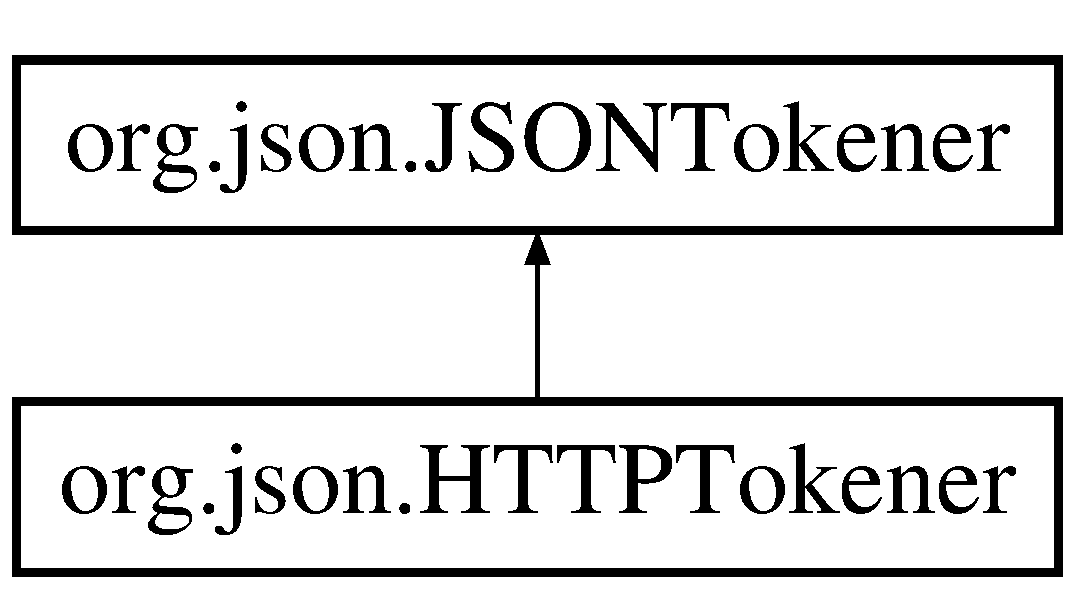
\includegraphics[height=2.000000cm]{classorg_1_1json_1_1_h_t_t_p_tokener}
\end{center}
\end{figure}
\subsection*{Public Member Functions}
\begin{DoxyCompactItemize}
\item 
\hyperlink{classorg_1_1json_1_1_h_t_t_p_tokener_a60475c4923ebf3ec28ed708bb0e4a6bc}{H\-T\-T\-P\-Tokener} (String string)
\item 
String \hyperlink{classorg_1_1json_1_1_h_t_t_p_tokener_a7189a17298ad2e09dce28e52bd5ccd07}{next\-Token} ()  throws J\-S\-O\-N\-Exception 
\end{DoxyCompactItemize}
\subsection*{Additional Inherited Members}


\subsection{Detailed Description}
The \hyperlink{classorg_1_1json_1_1_h_t_t_p_tokener}{H\-T\-T\-P\-Tokener} extends the \hyperlink{classorg_1_1json_1_1_j_s_o_n_tokener}{J\-S\-O\-N\-Tokener} to provide additional methods for the parsing of \hyperlink{classorg_1_1json_1_1_h_t_t_p}{H\-T\-T\-P} headers. \begin{DoxyAuthor}{Author}
J\-S\-O\-N.\-org 
\end{DoxyAuthor}
\begin{DoxyVersion}{Version}
2012-\/11-\/13 
\end{DoxyVersion}


Definition at line 33 of file H\-T\-T\-P\-Tokener.\-java.



\subsection{Constructor \& Destructor Documentation}
\hypertarget{classorg_1_1json_1_1_h_t_t_p_tokener_a60475c4923ebf3ec28ed708bb0e4a6bc}{\index{org\-::json\-::\-H\-T\-T\-P\-Tokener@{org\-::json\-::\-H\-T\-T\-P\-Tokener}!H\-T\-T\-P\-Tokener@{H\-T\-T\-P\-Tokener}}
\index{H\-T\-T\-P\-Tokener@{H\-T\-T\-P\-Tokener}!org::json::HTTPTokener@{org\-::json\-::\-H\-T\-T\-P\-Tokener}}
\subsubsection[{H\-T\-T\-P\-Tokener}]{\setlength{\rightskip}{0pt plus 5cm}org.\-json.\-H\-T\-T\-P\-Tokener.\-H\-T\-T\-P\-Tokener (
\begin{DoxyParamCaption}
\item[{String}]{string}
\end{DoxyParamCaption}
)}}\label{classorg_1_1json_1_1_h_t_t_p_tokener_a60475c4923ebf3ec28ed708bb0e4a6bc}
Construct an \hyperlink{classorg_1_1json_1_1_h_t_t_p_tokener}{H\-T\-T\-P\-Tokener} from a string. 
\begin{DoxyParams}{Parameters}
{\em string} & A source string. \\
\hline
\end{DoxyParams}


Definition at line 39 of file H\-T\-T\-P\-Tokener.\-java.


\begin{DoxyCode}
39                                       \{
40         super(\textcolor{keywordtype}{string});
41     \}
\end{DoxyCode}


\subsection{Member Function Documentation}
\hypertarget{classorg_1_1json_1_1_h_t_t_p_tokener_a7189a17298ad2e09dce28e52bd5ccd07}{\index{org\-::json\-::\-H\-T\-T\-P\-Tokener@{org\-::json\-::\-H\-T\-T\-P\-Tokener}!next\-Token@{next\-Token}}
\index{next\-Token@{next\-Token}!org::json::HTTPTokener@{org\-::json\-::\-H\-T\-T\-P\-Tokener}}
\subsubsection[{next\-Token}]{\setlength{\rightskip}{0pt plus 5cm}String org.\-json.\-H\-T\-T\-P\-Tokener.\-next\-Token (
\begin{DoxyParamCaption}
{}
\end{DoxyParamCaption}
) throws {\bf J\-S\-O\-N\-Exception}}}\label{classorg_1_1json_1_1_h_t_t_p_tokener_a7189a17298ad2e09dce28e52bd5ccd07}
Get the next token or string. This is used in parsing \hyperlink{classorg_1_1json_1_1_h_t_t_p}{H\-T\-T\-P} headers. 
\begin{DoxyExceptions}{Exceptions}
{\em \hyperlink{classorg_1_1json_1_1_j_s_o_n_exception}{J\-S\-O\-N\-Exception}} & \\
\hline
\end{DoxyExceptions}
\begin{DoxyReturn}{Returns}
A String. 
\end{DoxyReturn}


Definition at line 49 of file H\-T\-T\-P\-Tokener.\-java.



References org.\-json.\-J\-S\-O\-N\-Tokener.\-next(), and org.\-json.\-J\-S\-O\-N\-Tokener.\-syntax\-Error().



Referenced by org.\-json.\-H\-T\-T\-P.\-to\-J\-S\-O\-N\-Object().


\begin{DoxyCode}
49                                                    \{
50         \textcolor{keywordtype}{char} c;
51         \textcolor{keywordtype}{char} q;
52         StringBuffer sb = \textcolor{keyword}{new} StringBuffer();
53         \textcolor{keywordflow}{do} \{
54             c = \hyperlink{classorg_1_1json_1_1_j_s_o_n_tokener_ae129753dbe43ea50aa34e3c06773fdfb}{next}();
55         \} \textcolor{keywordflow}{while} (Character.isWhitespace(c));
56         \textcolor{keywordflow}{if} (c == \textcolor{charliteral}{'"'} || c == \textcolor{charliteral}{'\(\backslash\)''}) \{
57             q = c;
58             \textcolor{keywordflow}{for} (;;) \{
59                 c = \hyperlink{classorg_1_1json_1_1_j_s_o_n_tokener_ae129753dbe43ea50aa34e3c06773fdfb}{next}();
60                 \textcolor{keywordflow}{if} (c < \textcolor{charliteral}{' '}) \{
61                     \textcolor{keywordflow}{throw} \hyperlink{classorg_1_1json_1_1_j_s_o_n_tokener_a467f559950c039f28394ce3a0d2659ca}{syntaxError}(\textcolor{stringliteral}{"Unterminated string."});
62                 \}
63                 \textcolor{keywordflow}{if} (c == q) \{
64                     \textcolor{keywordflow}{return} sb.toString();
65                 \}
66                 sb.append(c);
67             \}
68         \}
69         \textcolor{keywordflow}{for} (;;) \{
70             \textcolor{keywordflow}{if} (c == 0 || Character.isWhitespace(c)) \{
71                 \textcolor{keywordflow}{return} sb.toString();
72             \}
73             sb.append(c);
74             c = \hyperlink{classorg_1_1json_1_1_j_s_o_n_tokener_ae129753dbe43ea50aa34e3c06773fdfb}{next}();
75         \}
76     \}
\end{DoxyCode}


The documentation for this class was generated from the following file\-:\begin{DoxyCompactItemize}
\item 
org/json/\hyperlink{_h_t_t_p_tokener_8java}{H\-T\-T\-P\-Tokener.\-java}\end{DoxyCompactItemize}

\hypertarget{classorg_1_1json_1_1_j_s_o_n_array}{\section{org.\-json.\-J\-S\-O\-N\-Array Class Reference}
\label{classorg_1_1json_1_1_j_s_o_n_array}\index{org.\-json.\-J\-S\-O\-N\-Array@{org.\-json.\-J\-S\-O\-N\-Array}}
}
\subsection*{Public Member Functions}
\begin{DoxyCompactItemize}
\item 
\hyperlink{classorg_1_1json_1_1_j_s_o_n_array_abf6f4be98df2bcc1fa7e08881bf1accd}{J\-S\-O\-N\-Array} ()
\item 
\hyperlink{classorg_1_1json_1_1_j_s_o_n_array_a9e8972d5f64b8fc6b7fca9169d29421a}{J\-S\-O\-N\-Array} (\hyperlink{classorg_1_1json_1_1_j_s_o_n_tokener}{J\-S\-O\-N\-Tokener} x)  throws J\-S\-O\-N\-Exception 
\item 
\hyperlink{classorg_1_1json_1_1_j_s_o_n_array_a62861e8a8afbae3fd6b637aeb444b2d4}{J\-S\-O\-N\-Array} (String source)  throws J\-S\-O\-N\-Exception 
\item 
\hyperlink{classorg_1_1json_1_1_j_s_o_n_array_ad8d5fa088a11f7fcb7ef328577c9c7a1}{J\-S\-O\-N\-Array} (Collection collection)
\item 
\hyperlink{classorg_1_1json_1_1_j_s_o_n_array_a22e9287f807d9846f4cb7d4bd300f2eb}{J\-S\-O\-N\-Array} (Object array)  throws J\-S\-O\-N\-Exception 
\item 
Object \hyperlink{classorg_1_1json_1_1_j_s_o_n_array_a3a8413753f53e0c0a5e008816c915eae}{get} (int index)  throws J\-S\-O\-N\-Exception 
\item 
boolean \hyperlink{classorg_1_1json_1_1_j_s_o_n_array_ac7b9da6fc6276ca0211a5bfb80d0f059}{get\-Boolean} (int index)  throws J\-S\-O\-N\-Exception 
\item 
double \hyperlink{classorg_1_1json_1_1_j_s_o_n_array_a1cd0e0c302e4acfe0393e6fbbc9a1c72}{get\-Double} (int index)  throws J\-S\-O\-N\-Exception 
\item 
int \hyperlink{classorg_1_1json_1_1_j_s_o_n_array_a1698dd185adbfa34dde18b2bef7f1e15}{get\-Int} (int index)  throws J\-S\-O\-N\-Exception 
\item 
\hyperlink{classorg_1_1json_1_1_j_s_o_n_array}{J\-S\-O\-N\-Array} \hyperlink{classorg_1_1json_1_1_j_s_o_n_array_a5d52943e4ca5982916b61aaa898dadad}{get\-J\-S\-O\-N\-Array} (int index)  throws J\-S\-O\-N\-Exception 
\item 
\hyperlink{classorg_1_1json_1_1_j_s_o_n_object}{J\-S\-O\-N\-Object} \hyperlink{classorg_1_1json_1_1_j_s_o_n_array_a7f3e6fc64826daba30f40964cd92e57e}{get\-J\-S\-O\-N\-Object} (int index)  throws J\-S\-O\-N\-Exception 
\item 
long \hyperlink{classorg_1_1json_1_1_j_s_o_n_array_a7d8cb28bbbcc4d3a3b00700a12331b94}{get\-Long} (int index)  throws J\-S\-O\-N\-Exception 
\item 
String \hyperlink{classorg_1_1json_1_1_j_s_o_n_array_a3b52ac3d94f48cdddf503e7872653591}{get\-String} (int index)  throws J\-S\-O\-N\-Exception 
\item 
boolean \hyperlink{classorg_1_1json_1_1_j_s_o_n_array_a53362530300e3530297eb8ddaf74098d}{is\-Null} (int index)
\item 
String \hyperlink{classorg_1_1json_1_1_j_s_o_n_array_ad0fbfe8fea05cdf7f06ddfe20db7c8c6}{join} (String separator)  throws J\-S\-O\-N\-Exception 
\item 
int \hyperlink{classorg_1_1json_1_1_j_s_o_n_array_a8382a78090007f650a02895ecbf3c8ec}{length} ()
\item 
Object \hyperlink{classorg_1_1json_1_1_j_s_o_n_array_a19aa83c80cded3d0a252c212ceca7954}{opt} (int index)
\item 
boolean \hyperlink{classorg_1_1json_1_1_j_s_o_n_array_a157f9232dea069ba4d201d1eba431084}{opt\-Boolean} (int index)
\item 
boolean \hyperlink{classorg_1_1json_1_1_j_s_o_n_array_adf119f56ddd47c4b9703f44efac4c3ef}{opt\-Boolean} (int index, boolean default\-Value)
\item 
double \hyperlink{classorg_1_1json_1_1_j_s_o_n_array_ae1cb586b1d073252a0ac07b6965f7a08}{opt\-Double} (int index)
\item 
double \hyperlink{classorg_1_1json_1_1_j_s_o_n_array_a0e12afede9c6e7be4ca467ce48171d17}{opt\-Double} (int index, double default\-Value)
\item 
int \hyperlink{classorg_1_1json_1_1_j_s_o_n_array_a10c76bdd9ef243702d62c0c92ea803fc}{opt\-Int} (int index)
\item 
int \hyperlink{classorg_1_1json_1_1_j_s_o_n_array_a820390cf8f7846a2363c59119e303a2d}{opt\-Int} (int index, int default\-Value)
\item 
\hyperlink{classorg_1_1json_1_1_j_s_o_n_array}{J\-S\-O\-N\-Array} \hyperlink{classorg_1_1json_1_1_j_s_o_n_array_af73e0318cfde76d4ade3cfc1bb99e325}{opt\-J\-S\-O\-N\-Array} (int index)
\item 
\hyperlink{classorg_1_1json_1_1_j_s_o_n_object}{J\-S\-O\-N\-Object} \hyperlink{classorg_1_1json_1_1_j_s_o_n_array_a21bcc36e0e4ce0f4659497db27d7081d}{opt\-J\-S\-O\-N\-Object} (int index)
\item 
long \hyperlink{classorg_1_1json_1_1_j_s_o_n_array_af38b848063c07f2a3218592bb595e722}{opt\-Long} (int index)
\item 
long \hyperlink{classorg_1_1json_1_1_j_s_o_n_array_a2c6ccec4ce5ab42e192e5686bc0ac03b}{opt\-Long} (int index, long default\-Value)
\item 
String \hyperlink{classorg_1_1json_1_1_j_s_o_n_array_aae00b0b37711915293a389a597f4adf7}{opt\-String} (int index)
\item 
String \hyperlink{classorg_1_1json_1_1_j_s_o_n_array_a81407977272f634afe7d278ecb9c44b5}{opt\-String} (int index, String default\-Value)
\item 
\hyperlink{classorg_1_1json_1_1_j_s_o_n_array}{J\-S\-O\-N\-Array} \hyperlink{classorg_1_1json_1_1_j_s_o_n_array_a54cc64e03735749abb69a05cf5b3ed68}{put} (boolean value)
\item 
\hyperlink{classorg_1_1json_1_1_j_s_o_n_array}{J\-S\-O\-N\-Array} \hyperlink{classorg_1_1json_1_1_j_s_o_n_array_a44f8b70a1f4d574bb4c10270c62f67bf}{put} (Collection value)
\item 
\hyperlink{classorg_1_1json_1_1_j_s_o_n_array}{J\-S\-O\-N\-Array} \hyperlink{classorg_1_1json_1_1_j_s_o_n_array_a0640a8fabd23294c4972a7884b1e3714}{put} (double value)  throws J\-S\-O\-N\-Exception 
\item 
\hyperlink{classorg_1_1json_1_1_j_s_o_n_array}{J\-S\-O\-N\-Array} \hyperlink{classorg_1_1json_1_1_j_s_o_n_array_a86a8ba6ff68f50faaad5c7070ef91f64}{put} (int value)
\item 
\hyperlink{classorg_1_1json_1_1_j_s_o_n_array}{J\-S\-O\-N\-Array} \hyperlink{classorg_1_1json_1_1_j_s_o_n_array_a3dd194b7438a41505fe1ff4cee0cd3fd}{put} (long value)
\item 
\hyperlink{classorg_1_1json_1_1_j_s_o_n_array}{J\-S\-O\-N\-Array} \hyperlink{classorg_1_1json_1_1_j_s_o_n_array_aa419be334b3ea1d04c3d4ba957f92ac8}{put} (Map value)
\item 
\hyperlink{classorg_1_1json_1_1_j_s_o_n_array}{J\-S\-O\-N\-Array} \hyperlink{classorg_1_1json_1_1_j_s_o_n_array_a184c04f20d200b83da5f70c05651949c}{put} (Object value)
\item 
\hyperlink{classorg_1_1json_1_1_j_s_o_n_array}{J\-S\-O\-N\-Array} \hyperlink{classorg_1_1json_1_1_j_s_o_n_array_a40deb37f82b54a44476a6a162ba55864}{put} (int index, boolean value)  throws J\-S\-O\-N\-Exception 
\item 
\hyperlink{classorg_1_1json_1_1_j_s_o_n_array}{J\-S\-O\-N\-Array} \hyperlink{classorg_1_1json_1_1_j_s_o_n_array_a378431a521ca31a67ea967754ef596f8}{put} (int index, Collection value)  throws J\-S\-O\-N\-Exception 
\item 
\hyperlink{classorg_1_1json_1_1_j_s_o_n_array}{J\-S\-O\-N\-Array} \hyperlink{classorg_1_1json_1_1_j_s_o_n_array_a44381e6efca784b131ff8d384f41447a}{put} (int index, double value)  throws J\-S\-O\-N\-Exception 
\item 
\hyperlink{classorg_1_1json_1_1_j_s_o_n_array}{J\-S\-O\-N\-Array} \hyperlink{classorg_1_1json_1_1_j_s_o_n_array_a2283abbc9a0e52077d0cce1a3ed8cd39}{put} (int index, int value)  throws J\-S\-O\-N\-Exception 
\item 
\hyperlink{classorg_1_1json_1_1_j_s_o_n_array}{J\-S\-O\-N\-Array} \hyperlink{classorg_1_1json_1_1_j_s_o_n_array_a8e84855241ff2c9af58f47043273956c}{put} (int index, long value)  throws J\-S\-O\-N\-Exception 
\item 
\hyperlink{classorg_1_1json_1_1_j_s_o_n_array}{J\-S\-O\-N\-Array} \hyperlink{classorg_1_1json_1_1_j_s_o_n_array_a95cada0cceecdff12a53c8ee1dd5cd35}{put} (int index, Map value)  throws J\-S\-O\-N\-Exception 
\item 
\hyperlink{classorg_1_1json_1_1_j_s_o_n_array}{J\-S\-O\-N\-Array} \hyperlink{classorg_1_1json_1_1_j_s_o_n_array_a5e2cb4652c3cfec3f955edd32e9aaf87}{put} (int index, Object value)  throws J\-S\-O\-N\-Exception 
\item 
Object \hyperlink{classorg_1_1json_1_1_j_s_o_n_array_ae5a2f41647bb60b10ae23e450a238f86}{remove} (int index)
\item 
\hyperlink{classorg_1_1json_1_1_j_s_o_n_object}{J\-S\-O\-N\-Object} \hyperlink{classorg_1_1json_1_1_j_s_o_n_array_a1b4d06dc69a1289bc2920c5780305962}{to\-J\-S\-O\-N\-Object} (\hyperlink{classorg_1_1json_1_1_j_s_o_n_array}{J\-S\-O\-N\-Array} names)  throws J\-S\-O\-N\-Exception 
\item 
String \hyperlink{classorg_1_1json_1_1_j_s_o_n_array_afc869e72ec78bf906683ab2f77cdba77}{to\-String} ()
\item 
String \hyperlink{classorg_1_1json_1_1_j_s_o_n_array_a4f18bcd5cb7b9f2b7c7918c55e0e9b10}{to\-String} (int indent\-Factor)  throws J\-S\-O\-N\-Exception 
\item 
Writer \hyperlink{classorg_1_1json_1_1_j_s_o_n_array_a28e509c7d8e5606e10a7a321c167aec8}{write} (Writer writer)  throws J\-S\-O\-N\-Exception 
\end{DoxyCompactItemize}
\subsection*{Package Functions}
\begin{DoxyCompactItemize}
\item 
Writer \hyperlink{classorg_1_1json_1_1_j_s_o_n_array_a1014b777a9b43800254b256354f79183}{write} (Writer writer, int indent\-Factor, int indent)  throws J\-S\-O\-N\-Exception 
\end{DoxyCompactItemize}
\subsection*{Private Attributes}
\begin{DoxyCompactItemize}
\item 
final Array\-List \hyperlink{classorg_1_1json_1_1_j_s_o_n_array_a0ae87624145bd5bec5fca66d37a5e794}{my\-Array\-List}
\end{DoxyCompactItemize}


\subsection{Detailed Description}
A \hyperlink{classorg_1_1json_1_1_j_s_o_n_array}{J\-S\-O\-N\-Array} is an ordered sequence of values. Its external text form is a string wrapped in square brackets with commas separating the values. The internal form is an object having {\ttfamily get} and {\ttfamily opt} methods for accessing the values by index, and {\ttfamily put} methods for adding or replacing values. The values can be any of these types\-: {\ttfamily Boolean}, {\ttfamily \hyperlink{classorg_1_1json_1_1_j_s_o_n_array}{J\-S\-O\-N\-Array}}, {\ttfamily \hyperlink{classorg_1_1json_1_1_j_s_o_n_object}{J\-S\-O\-N\-Object}}, {\ttfamily Number}, {\ttfamily String}, or the {\ttfamily \hyperlink{classorg_1_1json_1_1_j_s_o_n_object_a01c74a31a1abfd34ab13beb9347855ac}{J\-S\-O\-N\-Object.\-N\-U\-L\-L} object}. 

The constructor can convert a J\-S\-O\-N text into a Java object. The {\ttfamily to\-String} method converts to J\-S\-O\-N text. 

A {\ttfamily get} method returns a value if one can be found, and throws an exception if one cannot be found. An {\ttfamily opt} method returns a default value instead of throwing an exception, and so is useful for obtaining optional values. 

The generic {\ttfamily \hyperlink{classorg_1_1json_1_1_j_s_o_n_array_a3a8413753f53e0c0a5e008816c915eae}{get()}} and {\ttfamily \hyperlink{classorg_1_1json_1_1_j_s_o_n_array_a19aa83c80cded3d0a252c212ceca7954}{opt()}} methods return an object which you can cast or query for type. There are also typed {\ttfamily get} and {\ttfamily opt} methods that do type checking and type coercion for you. 

The texts produced by the {\ttfamily to\-String} methods strictly conform to J\-S\-O\-N syntax rules. The constructors are more forgiving in the texts they will accept\-: 
\begin{DoxyItemize}
\item An extra {\ttfamily ,}~
\footnotesize (comma)
\normalsize  may appear just before the closing bracket. 
\item The {\ttfamily null} value will be inserted when there is {\ttfamily ,} ~
\footnotesize (comma)
\normalsize  elision. 
\item Strings may be quoted with {\ttfamily '}~
\footnotesize (single quote)
\normalsize . 
\item Strings do not need to be quoted at all if they do not begin with a quote or single quote, and if they do not contain leading or trailing spaces, and if they do not contain any of these characters\-: {\ttfamily \{ \} \mbox{[} \mbox{]} / \textbackslash{} \-: , \#} and if they do not look like numbers and if they are not the reserved words {\ttfamily true}, {\ttfamily false}, or {\ttfamily null}. 
\end{DoxyItemize}

\begin{DoxyAuthor}{Author}
J\-S\-O\-N.\-org 
\end{DoxyAuthor}
\begin{DoxyVersion}{Version}
2013-\/04-\/18 
\end{DoxyVersion}


Definition at line 80 of file J\-S\-O\-N\-Array.\-java.



\subsection{Constructor \& Destructor Documentation}
\hypertarget{classorg_1_1json_1_1_j_s_o_n_array_abf6f4be98df2bcc1fa7e08881bf1accd}{\index{org\-::json\-::\-J\-S\-O\-N\-Array@{org\-::json\-::\-J\-S\-O\-N\-Array}!J\-S\-O\-N\-Array@{J\-S\-O\-N\-Array}}
\index{J\-S\-O\-N\-Array@{J\-S\-O\-N\-Array}!org::json::JSONArray@{org\-::json\-::\-J\-S\-O\-N\-Array}}
\subsubsection[{J\-S\-O\-N\-Array}]{\setlength{\rightskip}{0pt plus 5cm}org.\-json.\-J\-S\-O\-N\-Array.\-J\-S\-O\-N\-Array (
\begin{DoxyParamCaption}
{}
\end{DoxyParamCaption}
)}}\label{classorg_1_1json_1_1_j_s_o_n_array_abf6f4be98df2bcc1fa7e08881bf1accd}
Construct an empty \hyperlink{classorg_1_1json_1_1_j_s_o_n_array}{J\-S\-O\-N\-Array}. 

Definition at line 90 of file J\-S\-O\-N\-Array.\-java.



References org.\-json.\-J\-S\-O\-N\-Array.\-my\-Array\-List.



Referenced by org.\-json.\-J\-S\-O\-N\-Array.\-opt\-J\-S\-O\-N\-Array(), and org.\-json.\-J\-S\-O\-N\-Array.\-put().


\begin{DoxyCode}
90                        \{
91         this.\hyperlink{classorg_1_1json_1_1_j_s_o_n_array_a0ae87624145bd5bec5fca66d37a5e794}{myArrayList} = \textcolor{keyword}{new} ArrayList();
92     \}
\end{DoxyCode}
\hypertarget{classorg_1_1json_1_1_j_s_o_n_array_a9e8972d5f64b8fc6b7fca9169d29421a}{\index{org\-::json\-::\-J\-S\-O\-N\-Array@{org\-::json\-::\-J\-S\-O\-N\-Array}!J\-S\-O\-N\-Array@{J\-S\-O\-N\-Array}}
\index{J\-S\-O\-N\-Array@{J\-S\-O\-N\-Array}!org::json::JSONArray@{org\-::json\-::\-J\-S\-O\-N\-Array}}
\subsubsection[{J\-S\-O\-N\-Array}]{\setlength{\rightskip}{0pt plus 5cm}org.\-json.\-J\-S\-O\-N\-Array.\-J\-S\-O\-N\-Array (
\begin{DoxyParamCaption}
\item[{{\bf J\-S\-O\-N\-Tokener}}]{x}
\end{DoxyParamCaption}
) throws {\bf J\-S\-O\-N\-Exception}}}\label{classorg_1_1json_1_1_j_s_o_n_array_a9e8972d5f64b8fc6b7fca9169d29421a}
Construct a \hyperlink{classorg_1_1json_1_1_j_s_o_n_array}{J\-S\-O\-N\-Array} from a \hyperlink{classorg_1_1json_1_1_j_s_o_n_tokener}{J\-S\-O\-N\-Tokener}.


\begin{DoxyParams}{Parameters}
{\em x} & A \hyperlink{classorg_1_1json_1_1_j_s_o_n_tokener}{J\-S\-O\-N\-Tokener} \\
\hline
\end{DoxyParams}

\begin{DoxyExceptions}{Exceptions}
{\em \hyperlink{classorg_1_1json_1_1_j_s_o_n_exception}{J\-S\-O\-N\-Exception}} & If there is a syntax error. \\
\hline
\end{DoxyExceptions}


Definition at line 102 of file J\-S\-O\-N\-Array.\-java.



References org.\-json.\-J\-S\-O\-N\-Array.\-my\-Array\-List, and org.\-json.\-J\-S\-O\-N\-Object.\-N\-U\-L\-L.


\begin{DoxyCode}
102                                                          \{
103         \textcolor{keyword}{this}();
104         \textcolor{keywordflow}{if} (x.nextClean() != \textcolor{charliteral}{'['}) \{
105             \textcolor{keywordflow}{throw} x.syntaxError(\textcolor{stringliteral}{"A JSONArray text must start with '['"});
106         \}
107         \textcolor{keywordflow}{if} (x.nextClean() != \textcolor{charliteral}{']'}) \{
108             x.back();
109             \textcolor{keywordflow}{for} (;;) \{
110                 \textcolor{keywordflow}{if} (x.nextClean() == \textcolor{charliteral}{','}) \{
111                     x.back();
112                     this.\hyperlink{classorg_1_1json_1_1_j_s_o_n_array_a0ae87624145bd5bec5fca66d37a5e794}{myArrayList}.add(JSONObject.NULL);
113                 \} \textcolor{keywordflow}{else} \{
114                     x.back();
115                     this.\hyperlink{classorg_1_1json_1_1_j_s_o_n_array_a0ae87624145bd5bec5fca66d37a5e794}{myArrayList}.add(x.nextValue());
116                 \}
117                 \textcolor{keywordflow}{switch} (x.nextClean()) \{
118                 \textcolor{keywordflow}{case} \textcolor{charliteral}{','}:
119                     \textcolor{keywordflow}{if} (x.nextClean() == \textcolor{charliteral}{']'}) \{
120                         \textcolor{keywordflow}{return};
121                     \}
122                     x.back();
123                     \textcolor{keywordflow}{break};
124                 \textcolor{keywordflow}{case} \textcolor{charliteral}{']'}:
125                     \textcolor{keywordflow}{return};
126                 \textcolor{keywordflow}{default}:
127                     \textcolor{keywordflow}{throw} x.syntaxError(\textcolor{stringliteral}{"Expected a ',' or ']'"});
128                 \}
129             \}
130         \}
131     \}
\end{DoxyCode}
\hypertarget{classorg_1_1json_1_1_j_s_o_n_array_a62861e8a8afbae3fd6b637aeb444b2d4}{\index{org\-::json\-::\-J\-S\-O\-N\-Array@{org\-::json\-::\-J\-S\-O\-N\-Array}!J\-S\-O\-N\-Array@{J\-S\-O\-N\-Array}}
\index{J\-S\-O\-N\-Array@{J\-S\-O\-N\-Array}!org::json::JSONArray@{org\-::json\-::\-J\-S\-O\-N\-Array}}
\subsubsection[{J\-S\-O\-N\-Array}]{\setlength{\rightskip}{0pt plus 5cm}org.\-json.\-J\-S\-O\-N\-Array.\-J\-S\-O\-N\-Array (
\begin{DoxyParamCaption}
\item[{String}]{source}
\end{DoxyParamCaption}
) throws {\bf J\-S\-O\-N\-Exception}}}\label{classorg_1_1json_1_1_j_s_o_n_array_a62861e8a8afbae3fd6b637aeb444b2d4}
Construct a \hyperlink{classorg_1_1json_1_1_j_s_o_n_array}{J\-S\-O\-N\-Array} from a source J\-S\-O\-N text.


\begin{DoxyParams}{Parameters}
{\em source} & A string that begins with {\ttfamily \mbox{[}}~
\footnotesize (left bracket)
\normalsize  and ends with {\ttfamily \mbox{]}} ~
\footnotesize (right bracket)
\normalsize . \\
\hline
\end{DoxyParams}

\begin{DoxyExceptions}{Exceptions}
{\em \hyperlink{classorg_1_1json_1_1_j_s_o_n_exception}{J\-S\-O\-N\-Exception}} & If there is a syntax error. \\
\hline
\end{DoxyExceptions}


Definition at line 143 of file J\-S\-O\-N\-Array.\-java.


\begin{DoxyCode}
143                                                          \{
144         \textcolor{keyword}{this}(\textcolor{keyword}{new} JSONTokener(source));
145     \}
\end{DoxyCode}
\hypertarget{classorg_1_1json_1_1_j_s_o_n_array_ad8d5fa088a11f7fcb7ef328577c9c7a1}{\index{org\-::json\-::\-J\-S\-O\-N\-Array@{org\-::json\-::\-J\-S\-O\-N\-Array}!J\-S\-O\-N\-Array@{J\-S\-O\-N\-Array}}
\index{J\-S\-O\-N\-Array@{J\-S\-O\-N\-Array}!org::json::JSONArray@{org\-::json\-::\-J\-S\-O\-N\-Array}}
\subsubsection[{J\-S\-O\-N\-Array}]{\setlength{\rightskip}{0pt plus 5cm}org.\-json.\-J\-S\-O\-N\-Array.\-J\-S\-O\-N\-Array (
\begin{DoxyParamCaption}
\item[{Collection}]{collection}
\end{DoxyParamCaption}
)}}\label{classorg_1_1json_1_1_j_s_o_n_array_ad8d5fa088a11f7fcb7ef328577c9c7a1}
Construct a \hyperlink{classorg_1_1json_1_1_j_s_o_n_array}{J\-S\-O\-N\-Array} from a Collection.


\begin{DoxyParams}{Parameters}
{\em collection} & A Collection. \\
\hline
\end{DoxyParams}


Definition at line 153 of file J\-S\-O\-N\-Array.\-java.



References org.\-json.\-J\-S\-O\-N\-Array.\-my\-Array\-List, and org.\-json.\-J\-S\-O\-N\-Object.\-wrap().


\begin{DoxyCode}
153                                             \{
154         this.\hyperlink{classorg_1_1json_1_1_j_s_o_n_array_a0ae87624145bd5bec5fca66d37a5e794}{myArrayList} = \textcolor{keyword}{new} ArrayList();
155         \textcolor{keywordflow}{if} (collection != null) \{
156             Iterator iter = collection.iterator();
157             \textcolor{keywordflow}{while} (iter.hasNext()) \{
158                 this.\hyperlink{classorg_1_1json_1_1_j_s_o_n_array_a0ae87624145bd5bec5fca66d37a5e794}{myArrayList}.add(JSONObject.wrap(iter.next()));
159             \}
160         \}
161     \}
\end{DoxyCode}
\hypertarget{classorg_1_1json_1_1_j_s_o_n_array_a22e9287f807d9846f4cb7d4bd300f2eb}{\index{org\-::json\-::\-J\-S\-O\-N\-Array@{org\-::json\-::\-J\-S\-O\-N\-Array}!J\-S\-O\-N\-Array@{J\-S\-O\-N\-Array}}
\index{J\-S\-O\-N\-Array@{J\-S\-O\-N\-Array}!org::json::JSONArray@{org\-::json\-::\-J\-S\-O\-N\-Array}}
\subsubsection[{J\-S\-O\-N\-Array}]{\setlength{\rightskip}{0pt plus 5cm}org.\-json.\-J\-S\-O\-N\-Array.\-J\-S\-O\-N\-Array (
\begin{DoxyParamCaption}
\item[{Object}]{array}
\end{DoxyParamCaption}
) throws {\bf J\-S\-O\-N\-Exception}}}\label{classorg_1_1json_1_1_j_s_o_n_array_a22e9287f807d9846f4cb7d4bd300f2eb}
Construct a \hyperlink{classorg_1_1json_1_1_j_s_o_n_array}{J\-S\-O\-N\-Array} from an array


\begin{DoxyExceptions}{Exceptions}
{\em \hyperlink{classorg_1_1json_1_1_j_s_o_n_exception}{J\-S\-O\-N\-Exception}} & If not an array. \\
\hline
\end{DoxyExceptions}


Definition at line 169 of file J\-S\-O\-N\-Array.\-java.



References org.\-json.\-J\-S\-O\-N\-Array.\-length(), org.\-json.\-J\-S\-O\-N\-Array.\-put(), and org.\-json.\-J\-S\-O\-N\-Object.\-wrap().


\begin{DoxyCode}
169                                                         \{
170         \textcolor{keyword}{this}();
171         \textcolor{keywordflow}{if} (array.getClass().isArray()) \{
172             \textcolor{keywordtype}{int} \hyperlink{classorg_1_1json_1_1_j_s_o_n_array_a8382a78090007f650a02895ecbf3c8ec}{length} = Array.getLength(array);
173             \textcolor{keywordflow}{for} (\textcolor{keywordtype}{int} i = 0; i < \hyperlink{classorg_1_1json_1_1_j_s_o_n_array_a8382a78090007f650a02895ecbf3c8ec}{length}; i += 1) \{
174                 this.\hyperlink{classorg_1_1json_1_1_j_s_o_n_array_a54cc64e03735749abb69a05cf5b3ed68}{put}(JSONObject.wrap(Array.get(array, i)));
175             \}
176         \} \textcolor{keywordflow}{else} \{
177             \textcolor{keywordflow}{throw} \textcolor{keyword}{new} JSONException(
178                     \textcolor{stringliteral}{"JSONArray initial value should be a string or collection or array."});
179         \}
180     \}
\end{DoxyCode}


\subsection{Member Function Documentation}
\hypertarget{classorg_1_1json_1_1_j_s_o_n_array_a3a8413753f53e0c0a5e008816c915eae}{\index{org\-::json\-::\-J\-S\-O\-N\-Array@{org\-::json\-::\-J\-S\-O\-N\-Array}!get@{get}}
\index{get@{get}!org::json::JSONArray@{org\-::json\-::\-J\-S\-O\-N\-Array}}
\subsubsection[{get}]{\setlength{\rightskip}{0pt plus 5cm}Object org.\-json.\-J\-S\-O\-N\-Array.\-get (
\begin{DoxyParamCaption}
\item[{int}]{index}
\end{DoxyParamCaption}
) throws {\bf J\-S\-O\-N\-Exception}}}\label{classorg_1_1json_1_1_j_s_o_n_array_a3a8413753f53e0c0a5e008816c915eae}
Get the object value associated with an index.


\begin{DoxyParams}{Parameters}
{\em index} & The index must be between 0 and \hyperlink{classorg_1_1json_1_1_j_s_o_n_array_a8382a78090007f650a02895ecbf3c8ec}{length()} -\/ 1. \\
\hline
\end{DoxyParams}
\begin{DoxyReturn}{Returns}
An object value. 
\end{DoxyReturn}

\begin{DoxyExceptions}{Exceptions}
{\em \hyperlink{classorg_1_1json_1_1_j_s_o_n_exception}{J\-S\-O\-N\-Exception}} & If there is no value for the index. \\
\hline
\end{DoxyExceptions}


Definition at line 191 of file J\-S\-O\-N\-Array.\-java.



References org.\-json.\-J\-S\-O\-N\-Array.\-opt().



Referenced by org.\-json.\-X\-M\-L.\-to\-String(), and org.\-json.\-J\-S\-O\-N\-M\-L.\-to\-String().


\begin{DoxyCode}
191                                                       \{
192         Object \textcolor{keywordtype}{object} = this.\hyperlink{classorg_1_1json_1_1_j_s_o_n_array_a19aa83c80cded3d0a252c212ceca7954}{opt}(index);
193         \textcolor{keywordflow}{if} (\textcolor{keywordtype}{object} == null) \{
194             \textcolor{keywordflow}{throw} \textcolor{keyword}{new} JSONException(\textcolor{stringliteral}{"JSONArray["} + index + \textcolor{stringliteral}{"] not found."});
195         \}
196         \textcolor{keywordflow}{return} object;
197     \}
\end{DoxyCode}
\hypertarget{classorg_1_1json_1_1_j_s_o_n_array_ac7b9da6fc6276ca0211a5bfb80d0f059}{\index{org\-::json\-::\-J\-S\-O\-N\-Array@{org\-::json\-::\-J\-S\-O\-N\-Array}!get\-Boolean@{get\-Boolean}}
\index{get\-Boolean@{get\-Boolean}!org::json::JSONArray@{org\-::json\-::\-J\-S\-O\-N\-Array}}
\subsubsection[{get\-Boolean}]{\setlength{\rightskip}{0pt plus 5cm}boolean org.\-json.\-J\-S\-O\-N\-Array.\-get\-Boolean (
\begin{DoxyParamCaption}
\item[{int}]{index}
\end{DoxyParamCaption}
) throws {\bf J\-S\-O\-N\-Exception}}}\label{classorg_1_1json_1_1_j_s_o_n_array_ac7b9da6fc6276ca0211a5bfb80d0f059}
Get the boolean value associated with an index. The string values \char`\"{}true\char`\"{} and \char`\"{}false\char`\"{} are converted to boolean.


\begin{DoxyParams}{Parameters}
{\em index} & The index must be between 0 and \hyperlink{classorg_1_1json_1_1_j_s_o_n_array_a8382a78090007f650a02895ecbf3c8ec}{length()} -\/ 1. \\
\hline
\end{DoxyParams}
\begin{DoxyReturn}{Returns}
The truth. 
\end{DoxyReturn}

\begin{DoxyExceptions}{Exceptions}
{\em \hyperlink{classorg_1_1json_1_1_j_s_o_n_exception}{J\-S\-O\-N\-Exception}} & If there is no value for the index or if the value is not convertible to boolean. \\
\hline
\end{DoxyExceptions}


Definition at line 210 of file J\-S\-O\-N\-Array.\-java.



Referenced by org.\-json.\-J\-S\-O\-N\-Array.\-opt\-Boolean().


\begin{DoxyCode}
210                                                               \{
211         Object \textcolor{keywordtype}{object} = this.\textcolor{keyword}{get}(index);
212         \textcolor{keywordflow}{if} (\textcolor{keywordtype}{object}.equals(Boolean.FALSE)
213                 || (\textcolor{keywordtype}{object} instanceof String && ((String) \textcolor{keywordtype}{object})
214                         .equalsIgnoreCase(\textcolor{stringliteral}{"false"}))) \{
215             \textcolor{keywordflow}{return} \textcolor{keyword}{false};
216         \} \textcolor{keywordflow}{else} \textcolor{keywordflow}{if} (\textcolor{keywordtype}{object}.equals(Boolean.TRUE)
217                 || (\textcolor{keywordtype}{object} instanceof String && ((String) \textcolor{keywordtype}{object})
218                         .equalsIgnoreCase(\textcolor{stringliteral}{"true"}))) \{
219             \textcolor{keywordflow}{return} \textcolor{keyword}{true};
220         \}
221         \textcolor{keywordflow}{throw} \textcolor{keyword}{new} JSONException(\textcolor{stringliteral}{"JSONArray["} + index + \textcolor{stringliteral}{"] is not a boolean."});
222     \}
\end{DoxyCode}
\hypertarget{classorg_1_1json_1_1_j_s_o_n_array_a1cd0e0c302e4acfe0393e6fbbc9a1c72}{\index{org\-::json\-::\-J\-S\-O\-N\-Array@{org\-::json\-::\-J\-S\-O\-N\-Array}!get\-Double@{get\-Double}}
\index{get\-Double@{get\-Double}!org::json::JSONArray@{org\-::json\-::\-J\-S\-O\-N\-Array}}
\subsubsection[{get\-Double}]{\setlength{\rightskip}{0pt plus 5cm}double org.\-json.\-J\-S\-O\-N\-Array.\-get\-Double (
\begin{DoxyParamCaption}
\item[{int}]{index}
\end{DoxyParamCaption}
) throws {\bf J\-S\-O\-N\-Exception}}}\label{classorg_1_1json_1_1_j_s_o_n_array_a1cd0e0c302e4acfe0393e6fbbc9a1c72}
Get the double value associated with an index.


\begin{DoxyParams}{Parameters}
{\em index} & The index must be between 0 and \hyperlink{classorg_1_1json_1_1_j_s_o_n_array_a8382a78090007f650a02895ecbf3c8ec}{length()} -\/ 1. \\
\hline
\end{DoxyParams}
\begin{DoxyReturn}{Returns}
The value. 
\end{DoxyReturn}

\begin{DoxyExceptions}{Exceptions}
{\em \hyperlink{classorg_1_1json_1_1_j_s_o_n_exception}{J\-S\-O\-N\-Exception}} & If the key is not found or if the value cannot be converted to a number. \\
\hline
\end{DoxyExceptions}


Definition at line 234 of file J\-S\-O\-N\-Array.\-java.



Referenced by org.\-json.\-J\-S\-O\-N\-Array.\-opt\-Double().


\begin{DoxyCode}
234                                                             \{
235         Object \textcolor{keywordtype}{object} = this.\textcolor{keyword}{get}(index);
236         \textcolor{keywordflow}{try} \{
237             \textcolor{keywordflow}{return} \textcolor{keywordtype}{object} instanceof Number ? ((Number) \textcolor{keywordtype}{object}).doubleValue()
238                     : Double.parseDouble((String) \textcolor{keywordtype}{object});
239         \} \textcolor{keywordflow}{catch} (Exception e) \{
240             \textcolor{keywordflow}{throw} \textcolor{keyword}{new} JSONException(\textcolor{stringliteral}{"JSONArray["} + index + \textcolor{stringliteral}{"] is not a number."});
241         \}
242     \}
\end{DoxyCode}
\hypertarget{classorg_1_1json_1_1_j_s_o_n_array_a1698dd185adbfa34dde18b2bef7f1e15}{\index{org\-::json\-::\-J\-S\-O\-N\-Array@{org\-::json\-::\-J\-S\-O\-N\-Array}!get\-Int@{get\-Int}}
\index{get\-Int@{get\-Int}!org::json::JSONArray@{org\-::json\-::\-J\-S\-O\-N\-Array}}
\subsubsection[{get\-Int}]{\setlength{\rightskip}{0pt plus 5cm}int org.\-json.\-J\-S\-O\-N\-Array.\-get\-Int (
\begin{DoxyParamCaption}
\item[{int}]{index}
\end{DoxyParamCaption}
) throws {\bf J\-S\-O\-N\-Exception}}}\label{classorg_1_1json_1_1_j_s_o_n_array_a1698dd185adbfa34dde18b2bef7f1e15}
Get the int value associated with an index.


\begin{DoxyParams}{Parameters}
{\em index} & The index must be between 0 and \hyperlink{classorg_1_1json_1_1_j_s_o_n_array_a8382a78090007f650a02895ecbf3c8ec}{length()} -\/ 1. \\
\hline
\end{DoxyParams}
\begin{DoxyReturn}{Returns}
The value. 
\end{DoxyReturn}

\begin{DoxyExceptions}{Exceptions}
{\em \hyperlink{classorg_1_1json_1_1_j_s_o_n_exception}{J\-S\-O\-N\-Exception}} & If the key is not found or if the value is not a number. \\
\hline
\end{DoxyExceptions}


Definition at line 253 of file J\-S\-O\-N\-Array.\-java.



Referenced by org.\-json.\-J\-S\-O\-N\-Array.\-opt\-Int().


\begin{DoxyCode}
253                                                       \{
254         Object \textcolor{keywordtype}{object} = this.\textcolor{keyword}{get}(index);
255         \textcolor{keywordflow}{try} \{
256             \textcolor{keywordflow}{return} \textcolor{keywordtype}{object} instanceof Number ? ((Number) \textcolor{keywordtype}{object}).intValue()
257                     : Integer.parseInt((String) \textcolor{keywordtype}{object});
258         \} \textcolor{keywordflow}{catch} (Exception e) \{
259             \textcolor{keywordflow}{throw} \textcolor{keyword}{new} JSONException(\textcolor{stringliteral}{"JSONArray["} + index + \textcolor{stringliteral}{"] is not a number."});
260         \}
261     \}
\end{DoxyCode}
\hypertarget{classorg_1_1json_1_1_j_s_o_n_array_a5d52943e4ca5982916b61aaa898dadad}{\index{org\-::json\-::\-J\-S\-O\-N\-Array@{org\-::json\-::\-J\-S\-O\-N\-Array}!get\-J\-S\-O\-N\-Array@{get\-J\-S\-O\-N\-Array}}
\index{get\-J\-S\-O\-N\-Array@{get\-J\-S\-O\-N\-Array}!org::json::JSONArray@{org\-::json\-::\-J\-S\-O\-N\-Array}}
\subsubsection[{get\-J\-S\-O\-N\-Array}]{\setlength{\rightskip}{0pt plus 5cm}{\bf J\-S\-O\-N\-Array} org.\-json.\-J\-S\-O\-N\-Array.\-get\-J\-S\-O\-N\-Array (
\begin{DoxyParamCaption}
\item[{int}]{index}
\end{DoxyParamCaption}
) throws {\bf J\-S\-O\-N\-Exception}}}\label{classorg_1_1json_1_1_j_s_o_n_array_a5d52943e4ca5982916b61aaa898dadad}
Get the \hyperlink{classorg_1_1json_1_1_j_s_o_n_array}{J\-S\-O\-N\-Array} associated with an index.


\begin{DoxyParams}{Parameters}
{\em index} & The index must be between 0 and \hyperlink{classorg_1_1json_1_1_j_s_o_n_array_a8382a78090007f650a02895ecbf3c8ec}{length()} -\/ 1. \\
\hline
\end{DoxyParams}
\begin{DoxyReturn}{Returns}
A \hyperlink{classorg_1_1json_1_1_j_s_o_n_array}{J\-S\-O\-N\-Array} value. 
\end{DoxyReturn}

\begin{DoxyExceptions}{Exceptions}
{\em \hyperlink{classorg_1_1json_1_1_j_s_o_n_exception}{J\-S\-O\-N\-Exception}} & If there is no value for the index. or if the value is not a \hyperlink{classorg_1_1json_1_1_j_s_o_n_array}{J\-S\-O\-N\-Array} \\
\hline
\end{DoxyExceptions}


Definition at line 273 of file J\-S\-O\-N\-Array.\-java.


\begin{DoxyCode}
273                                                                   \{
274         Object \textcolor{keywordtype}{object} = this.\textcolor{keyword}{get}(index);
275         \textcolor{keywordflow}{if} (\textcolor{keywordtype}{object} instanceof \hyperlink{classorg_1_1json_1_1_j_s_o_n_array_abf6f4be98df2bcc1fa7e08881bf1accd}{JSONArray}) \{
276             \textcolor{keywordflow}{return} (JSONArray) object;
277         \}
278         \textcolor{keywordflow}{throw} \textcolor{keyword}{new} JSONException(\textcolor{stringliteral}{"JSONArray["} + index + \textcolor{stringliteral}{"] is not a JSONArray."});
279     \}
\end{DoxyCode}
\hypertarget{classorg_1_1json_1_1_j_s_o_n_array_a7f3e6fc64826daba30f40964cd92e57e}{\index{org\-::json\-::\-J\-S\-O\-N\-Array@{org\-::json\-::\-J\-S\-O\-N\-Array}!get\-J\-S\-O\-N\-Object@{get\-J\-S\-O\-N\-Object}}
\index{get\-J\-S\-O\-N\-Object@{get\-J\-S\-O\-N\-Object}!org::json::JSONArray@{org\-::json\-::\-J\-S\-O\-N\-Array}}
\subsubsection[{get\-J\-S\-O\-N\-Object}]{\setlength{\rightskip}{0pt plus 5cm}{\bf J\-S\-O\-N\-Object} org.\-json.\-J\-S\-O\-N\-Array.\-get\-J\-S\-O\-N\-Object (
\begin{DoxyParamCaption}
\item[{int}]{index}
\end{DoxyParamCaption}
) throws {\bf J\-S\-O\-N\-Exception}}}\label{classorg_1_1json_1_1_j_s_o_n_array_a7f3e6fc64826daba30f40964cd92e57e}
Get the \hyperlink{classorg_1_1json_1_1_j_s_o_n_object}{J\-S\-O\-N\-Object} associated with an index.


\begin{DoxyParams}{Parameters}
{\em index} & subscript \\
\hline
\end{DoxyParams}
\begin{DoxyReturn}{Returns}
A \hyperlink{classorg_1_1json_1_1_j_s_o_n_object}{J\-S\-O\-N\-Object} value. 
\end{DoxyReturn}

\begin{DoxyExceptions}{Exceptions}
{\em \hyperlink{classorg_1_1json_1_1_j_s_o_n_exception}{J\-S\-O\-N\-Exception}} & If there is no value for the index or if the value is not a \hyperlink{classorg_1_1json_1_1_j_s_o_n_object}{J\-S\-O\-N\-Object} \\
\hline
\end{DoxyExceptions}


Definition at line 291 of file J\-S\-O\-N\-Array.\-java.



Referenced by org.\-facebook.\-crawler.\-Facebook\-Json\-Parser.\-crawl\-Group(), org.\-facebook.\-crawler.\-Facebook\-Json\-Parser.\-crawl\-User(), and Json\-Reader.\-main().


\begin{DoxyCode}
291                                                                     \{
292         Object \textcolor{keywordtype}{object} = this.\textcolor{keyword}{get}(index);
293         \textcolor{keywordflow}{if} (\textcolor{keywordtype}{object} instanceof JSONObject) \{
294             \textcolor{keywordflow}{return} (JSONObject) object;
295         \}
296         \textcolor{keywordflow}{throw} \textcolor{keyword}{new} JSONException(\textcolor{stringliteral}{"JSONArray["} + index + \textcolor{stringliteral}{"] is not a JSONObject."});
297     \}
\end{DoxyCode}
\hypertarget{classorg_1_1json_1_1_j_s_o_n_array_a7d8cb28bbbcc4d3a3b00700a12331b94}{\index{org\-::json\-::\-J\-S\-O\-N\-Array@{org\-::json\-::\-J\-S\-O\-N\-Array}!get\-Long@{get\-Long}}
\index{get\-Long@{get\-Long}!org::json::JSONArray@{org\-::json\-::\-J\-S\-O\-N\-Array}}
\subsubsection[{get\-Long}]{\setlength{\rightskip}{0pt plus 5cm}long org.\-json.\-J\-S\-O\-N\-Array.\-get\-Long (
\begin{DoxyParamCaption}
\item[{int}]{index}
\end{DoxyParamCaption}
) throws {\bf J\-S\-O\-N\-Exception}}}\label{classorg_1_1json_1_1_j_s_o_n_array_a7d8cb28bbbcc4d3a3b00700a12331b94}
Get the long value associated with an index.


\begin{DoxyParams}{Parameters}
{\em index} & The index must be between 0 and \hyperlink{classorg_1_1json_1_1_j_s_o_n_array_a8382a78090007f650a02895ecbf3c8ec}{length()} -\/ 1. \\
\hline
\end{DoxyParams}
\begin{DoxyReturn}{Returns}
The value. 
\end{DoxyReturn}

\begin{DoxyExceptions}{Exceptions}
{\em \hyperlink{classorg_1_1json_1_1_j_s_o_n_exception}{J\-S\-O\-N\-Exception}} & If the key is not found or if the value cannot be converted to a number. \\
\hline
\end{DoxyExceptions}


Definition at line 309 of file J\-S\-O\-N\-Array.\-java.



Referenced by org.\-json.\-J\-S\-O\-N\-Array.\-opt\-Long().


\begin{DoxyCode}
309                                                         \{
310         Object \textcolor{keywordtype}{object} = this.\textcolor{keyword}{get}(index);
311         \textcolor{keywordflow}{try} \{
312             \textcolor{keywordflow}{return} \textcolor{keywordtype}{object} instanceof Number ? ((Number) \textcolor{keywordtype}{object}).longValue()
313                     : Long.parseLong((String) \textcolor{keywordtype}{object});
314         \} \textcolor{keywordflow}{catch} (Exception e) \{
315             \textcolor{keywordflow}{throw} \textcolor{keyword}{new} JSONException(\textcolor{stringliteral}{"JSONArray["} + index + \textcolor{stringliteral}{"] is not a number."});
316         \}
317     \}
\end{DoxyCode}
\hypertarget{classorg_1_1json_1_1_j_s_o_n_array_a3b52ac3d94f48cdddf503e7872653591}{\index{org\-::json\-::\-J\-S\-O\-N\-Array@{org\-::json\-::\-J\-S\-O\-N\-Array}!get\-String@{get\-String}}
\index{get\-String@{get\-String}!org::json::JSONArray@{org\-::json\-::\-J\-S\-O\-N\-Array}}
\subsubsection[{get\-String}]{\setlength{\rightskip}{0pt plus 5cm}String org.\-json.\-J\-S\-O\-N\-Array.\-get\-String (
\begin{DoxyParamCaption}
\item[{int}]{index}
\end{DoxyParamCaption}
) throws {\bf J\-S\-O\-N\-Exception}}}\label{classorg_1_1json_1_1_j_s_o_n_array_a3b52ac3d94f48cdddf503e7872653591}
Get the string associated with an index.


\begin{DoxyParams}{Parameters}
{\em index} & The index must be between 0 and \hyperlink{classorg_1_1json_1_1_j_s_o_n_array_a8382a78090007f650a02895ecbf3c8ec}{length()} -\/ 1. \\
\hline
\end{DoxyParams}
\begin{DoxyReturn}{Returns}
A string value. 
\end{DoxyReturn}

\begin{DoxyExceptions}{Exceptions}
{\em \hyperlink{classorg_1_1json_1_1_j_s_o_n_exception}{J\-S\-O\-N\-Exception}} & If there is no string value for the index. \\
\hline
\end{DoxyExceptions}


Definition at line 328 of file J\-S\-O\-N\-Array.\-java.



Referenced by org.\-facebook.\-crawler.\-Facebook\-Json\-Parser.\-crawl\-User(), Json\-Reader.\-main(), and org.\-json.\-J\-S\-O\-N\-Object.\-to\-J\-S\-O\-N\-Array().


\begin{DoxyCode}
328                                                             \{
329         Object \textcolor{keywordtype}{object} = this.\textcolor{keyword}{get}(index);
330         \textcolor{keywordflow}{if} (\textcolor{keywordtype}{object} instanceof String) \{
331             \textcolor{keywordflow}{return} (String) object;
332         \}
333         \textcolor{keywordflow}{throw} \textcolor{keyword}{new} JSONException(\textcolor{stringliteral}{"JSONArray["} + index + \textcolor{stringliteral}{"] not a string."});
334     \}
\end{DoxyCode}
\hypertarget{classorg_1_1json_1_1_j_s_o_n_array_a53362530300e3530297eb8ddaf74098d}{\index{org\-::json\-::\-J\-S\-O\-N\-Array@{org\-::json\-::\-J\-S\-O\-N\-Array}!is\-Null@{is\-Null}}
\index{is\-Null@{is\-Null}!org::json::JSONArray@{org\-::json\-::\-J\-S\-O\-N\-Array}}
\subsubsection[{is\-Null}]{\setlength{\rightskip}{0pt plus 5cm}boolean org.\-json.\-J\-S\-O\-N\-Array.\-is\-Null (
\begin{DoxyParamCaption}
\item[{int}]{index}
\end{DoxyParamCaption}
)}}\label{classorg_1_1json_1_1_j_s_o_n_array_a53362530300e3530297eb8ddaf74098d}
Determine if the value is null.


\begin{DoxyParams}{Parameters}
{\em index} & The index must be between 0 and \hyperlink{classorg_1_1json_1_1_j_s_o_n_array_a8382a78090007f650a02895ecbf3c8ec}{length()} -\/ 1. \\
\hline
\end{DoxyParams}
\begin{DoxyReturn}{Returns}
true if the value at the index is null, or if there is no value. 
\end{DoxyReturn}


Definition at line 343 of file J\-S\-O\-N\-Array.\-java.



References org.\-json.\-J\-S\-O\-N\-Object.\-N\-U\-L\-L, and org.\-json.\-J\-S\-O\-N\-Array.\-opt().


\begin{DoxyCode}
343                                      \{
344         \textcolor{keywordflow}{return} JSONObject.NULL.equals(this.\hyperlink{classorg_1_1json_1_1_j_s_o_n_array_a19aa83c80cded3d0a252c212ceca7954}{opt}(index));
345     \}
\end{DoxyCode}
\hypertarget{classorg_1_1json_1_1_j_s_o_n_array_ad0fbfe8fea05cdf7f06ddfe20db7c8c6}{\index{org\-::json\-::\-J\-S\-O\-N\-Array@{org\-::json\-::\-J\-S\-O\-N\-Array}!join@{join}}
\index{join@{join}!org::json::JSONArray@{org\-::json\-::\-J\-S\-O\-N\-Array}}
\subsubsection[{join}]{\setlength{\rightskip}{0pt plus 5cm}String org.\-json.\-J\-S\-O\-N\-Array.\-join (
\begin{DoxyParamCaption}
\item[{String}]{separator}
\end{DoxyParamCaption}
) throws {\bf J\-S\-O\-N\-Exception}}}\label{classorg_1_1json_1_1_j_s_o_n_array_ad0fbfe8fea05cdf7f06ddfe20db7c8c6}
Make a string from the contents of this \hyperlink{classorg_1_1json_1_1_j_s_o_n_array}{J\-S\-O\-N\-Array}. The {\ttfamily separator} string is inserted between each element. Warning\-: This method assumes that the data structure is acyclical.


\begin{DoxyParams}{Parameters}
{\em separator} & A string that will be inserted between the elements. \\
\hline
\end{DoxyParams}
\begin{DoxyReturn}{Returns}
a string. 
\end{DoxyReturn}

\begin{DoxyExceptions}{Exceptions}
{\em \hyperlink{classorg_1_1json_1_1_j_s_o_n_exception}{J\-S\-O\-N\-Exception}} & If the array contains an invalid number. \\
\hline
\end{DoxyExceptions}


Definition at line 358 of file J\-S\-O\-N\-Array.\-java.



References org.\-json.\-J\-S\-O\-N\-Array.\-length(), and org.\-json.\-J\-S\-O\-N\-Object.\-value\-To\-String().


\begin{DoxyCode}
358                                                               \{
359         \textcolor{keywordtype}{int} len = this.\hyperlink{classorg_1_1json_1_1_j_s_o_n_array_a8382a78090007f650a02895ecbf3c8ec}{length}();
360         StringBuffer sb = \textcolor{keyword}{new} StringBuffer();
361 
362         \textcolor{keywordflow}{for} (\textcolor{keywordtype}{int} i = 0; i < len; i += 1) \{
363             \textcolor{keywordflow}{if} (i > 0) \{
364                 sb.append(separator);
365             \}
366             sb.append(JSONObject.valueToString(\textcolor{keyword}{this}.myArrayList.get(i)));
367         \}
368         \textcolor{keywordflow}{return} sb.toString();
369     \}
\end{DoxyCode}
\hypertarget{classorg_1_1json_1_1_j_s_o_n_array_a8382a78090007f650a02895ecbf3c8ec}{\index{org\-::json\-::\-J\-S\-O\-N\-Array@{org\-::json\-::\-J\-S\-O\-N\-Array}!length@{length}}
\index{length@{length}!org::json::JSONArray@{org\-::json\-::\-J\-S\-O\-N\-Array}}
\subsubsection[{length}]{\setlength{\rightskip}{0pt plus 5cm}int org.\-json.\-J\-S\-O\-N\-Array.\-length (
\begin{DoxyParamCaption}
{}
\end{DoxyParamCaption}
)}}\label{classorg_1_1json_1_1_j_s_o_n_array_a8382a78090007f650a02895ecbf3c8ec}
Get the number of elements in the \hyperlink{classorg_1_1json_1_1_j_s_o_n_array}{J\-S\-O\-N\-Array}, included nulls.

\begin{DoxyReturn}{Returns}
The length (or size). 
\end{DoxyReturn}


Definition at line 376 of file J\-S\-O\-N\-Array.\-java.



References org.\-json.\-J\-S\-O\-N\-Array.\-my\-Array\-List.



Referenced by org.\-facebook.\-crawler.\-Facebook\-Json\-Parser.\-crawl\-Group(), org.\-facebook.\-crawler.\-Facebook\-Json\-Parser.\-crawl\-User(), org.\-json.\-J\-S\-O\-N\-Array.\-join(), org.\-json.\-J\-S\-O\-N\-Array.\-J\-S\-O\-N\-Array(), Json\-Reader.\-main(), org.\-json.\-J\-S\-O\-N\-Object.\-names(), org.\-json.\-J\-S\-O\-N\-Array.\-opt(), org.\-json.\-J\-S\-O\-N\-M\-L.\-parse(), org.\-json.\-J\-S\-O\-N\-Array.\-put(), org.\-json.\-C\-D\-L.\-row\-To\-J\-S\-O\-N\-Array(), org.\-json.\-C\-D\-L.\-row\-To\-String(), org.\-json.\-C\-D\-L.\-to\-J\-S\-O\-N\-Array(), org.\-json.\-J\-S\-O\-N\-Object.\-to\-J\-S\-O\-N\-Array(), org.\-json.\-J\-S\-O\-N\-Array.\-to\-J\-S\-O\-N\-Object(), org.\-json.\-X\-M\-L.\-to\-String(), org.\-json.\-J\-S\-O\-N\-M\-L.\-to\-String(), and org.\-json.\-J\-S\-O\-N\-Array.\-write().


\begin{DoxyCode}
376                         \{
377         \textcolor{keywordflow}{return} this.\hyperlink{classorg_1_1json_1_1_j_s_o_n_array_a0ae87624145bd5bec5fca66d37a5e794}{myArrayList}.size();
378     \}
\end{DoxyCode}
\hypertarget{classorg_1_1json_1_1_j_s_o_n_array_a19aa83c80cded3d0a252c212ceca7954}{\index{org\-::json\-::\-J\-S\-O\-N\-Array@{org\-::json\-::\-J\-S\-O\-N\-Array}!opt@{opt}}
\index{opt@{opt}!org::json::JSONArray@{org\-::json\-::\-J\-S\-O\-N\-Array}}
\subsubsection[{opt}]{\setlength{\rightskip}{0pt plus 5cm}Object org.\-json.\-J\-S\-O\-N\-Array.\-opt (
\begin{DoxyParamCaption}
\item[{int}]{index}
\end{DoxyParamCaption}
)}}\label{classorg_1_1json_1_1_j_s_o_n_array_a19aa83c80cded3d0a252c212ceca7954}
Get the optional object value associated with an index.


\begin{DoxyParams}{Parameters}
{\em index} & The index must be between 0 and \hyperlink{classorg_1_1json_1_1_j_s_o_n_array_a8382a78090007f650a02895ecbf3c8ec}{length()} -\/ 1. \\
\hline
\end{DoxyParams}
\begin{DoxyReturn}{Returns}
An object value, or null if there is no object at that index. 
\end{DoxyReturn}


Definition at line 387 of file J\-S\-O\-N\-Array.\-java.



References org.\-json.\-J\-S\-O\-N\-Array.\-length(), and org.\-json.\-J\-S\-O\-N\-Array.\-my\-Array\-List.



Referenced by org.\-json.\-J\-S\-O\-N\-Array.\-get(), org.\-json.\-J\-S\-O\-N\-Array.\-is\-Null(), org.\-json.\-J\-S\-O\-N\-Array.\-opt\-J\-S\-O\-N\-Array(), org.\-json.\-J\-S\-O\-N\-Array.\-opt\-J\-S\-O\-N\-Object(), org.\-json.\-J\-S\-O\-N\-Array.\-opt\-String(), org.\-json.\-J\-S\-O\-N\-Array.\-remove(), org.\-json.\-C\-D\-L.\-row\-To\-String(), org.\-json.\-J\-S\-O\-N\-Array.\-to\-J\-S\-O\-N\-Object(), and org.\-json.\-X\-M\-L.\-to\-String().


\begin{DoxyCode}
387                                  \{
388         \textcolor{keywordflow}{return} (index < 0 || index >= this.\hyperlink{classorg_1_1json_1_1_j_s_o_n_array_a8382a78090007f650a02895ecbf3c8ec}{length}()) ? null : this.
      \hyperlink{classorg_1_1json_1_1_j_s_o_n_array_a0ae87624145bd5bec5fca66d37a5e794}{myArrayList}
389                 .get(index);
390     \}
\end{DoxyCode}
\hypertarget{classorg_1_1json_1_1_j_s_o_n_array_a157f9232dea069ba4d201d1eba431084}{\index{org\-::json\-::\-J\-S\-O\-N\-Array@{org\-::json\-::\-J\-S\-O\-N\-Array}!opt\-Boolean@{opt\-Boolean}}
\index{opt\-Boolean@{opt\-Boolean}!org::json::JSONArray@{org\-::json\-::\-J\-S\-O\-N\-Array}}
\subsubsection[{opt\-Boolean}]{\setlength{\rightskip}{0pt plus 5cm}boolean org.\-json.\-J\-S\-O\-N\-Array.\-opt\-Boolean (
\begin{DoxyParamCaption}
\item[{int}]{index}
\end{DoxyParamCaption}
)}}\label{classorg_1_1json_1_1_j_s_o_n_array_a157f9232dea069ba4d201d1eba431084}
Get the optional boolean value associated with an index. It returns false if there is no value at that index, or if the value is not Boolean.\-T\-R\-U\-E or the String \char`\"{}true\char`\"{}.


\begin{DoxyParams}{Parameters}
{\em index} & The index must be between 0 and \hyperlink{classorg_1_1json_1_1_j_s_o_n_array_a8382a78090007f650a02895ecbf3c8ec}{length()} -\/ 1. \\
\hline
\end{DoxyParams}
\begin{DoxyReturn}{Returns}
The truth. 
\end{DoxyReturn}


Definition at line 401 of file J\-S\-O\-N\-Array.\-java.


\begin{DoxyCode}
401                                          \{
402         \textcolor{keywordflow}{return} this.\hyperlink{classorg_1_1json_1_1_j_s_o_n_array_a157f9232dea069ba4d201d1eba431084}{optBoolean}(index, \textcolor{keyword}{false});
403     \}
\end{DoxyCode}
\hypertarget{classorg_1_1json_1_1_j_s_o_n_array_adf119f56ddd47c4b9703f44efac4c3ef}{\index{org\-::json\-::\-J\-S\-O\-N\-Array@{org\-::json\-::\-J\-S\-O\-N\-Array}!opt\-Boolean@{opt\-Boolean}}
\index{opt\-Boolean@{opt\-Boolean}!org::json::JSONArray@{org\-::json\-::\-J\-S\-O\-N\-Array}}
\subsubsection[{opt\-Boolean}]{\setlength{\rightskip}{0pt plus 5cm}boolean org.\-json.\-J\-S\-O\-N\-Array.\-opt\-Boolean (
\begin{DoxyParamCaption}
\item[{int}]{index, }
\item[{boolean}]{default\-Value}
\end{DoxyParamCaption}
)}}\label{classorg_1_1json_1_1_j_s_o_n_array_adf119f56ddd47c4b9703f44efac4c3ef}
Get the optional boolean value associated with an index. It returns the default\-Value if there is no value at that index or if it is not a Boolean or the String \char`\"{}true\char`\"{} or \char`\"{}false\char`\"{} (case insensitive).


\begin{DoxyParams}{Parameters}
{\em index} & The index must be between 0 and \hyperlink{classorg_1_1json_1_1_j_s_o_n_array_a8382a78090007f650a02895ecbf3c8ec}{length()} -\/ 1. \\
\hline
{\em default\-Value} & A boolean default. \\
\hline
\end{DoxyParams}
\begin{DoxyReturn}{Returns}
The truth. 
\end{DoxyReturn}


Definition at line 416 of file J\-S\-O\-N\-Array.\-java.



References org.\-json.\-J\-S\-O\-N\-Array.\-get\-Boolean().


\begin{DoxyCode}
416                                                                \{
417         \textcolor{keywordflow}{try} \{
418             \textcolor{keywordflow}{return} this.\hyperlink{classorg_1_1json_1_1_j_s_o_n_array_ac7b9da6fc6276ca0211a5bfb80d0f059}{getBoolean}(index);
419         \} \textcolor{keywordflow}{catch} (Exception e) \{
420             \textcolor{keywordflow}{return} defaultValue;
421         \}
422     \}
\end{DoxyCode}
\hypertarget{classorg_1_1json_1_1_j_s_o_n_array_ae1cb586b1d073252a0ac07b6965f7a08}{\index{org\-::json\-::\-J\-S\-O\-N\-Array@{org\-::json\-::\-J\-S\-O\-N\-Array}!opt\-Double@{opt\-Double}}
\index{opt\-Double@{opt\-Double}!org::json::JSONArray@{org\-::json\-::\-J\-S\-O\-N\-Array}}
\subsubsection[{opt\-Double}]{\setlength{\rightskip}{0pt plus 5cm}double org.\-json.\-J\-S\-O\-N\-Array.\-opt\-Double (
\begin{DoxyParamCaption}
\item[{int}]{index}
\end{DoxyParamCaption}
)}}\label{classorg_1_1json_1_1_j_s_o_n_array_ae1cb586b1d073252a0ac07b6965f7a08}
Get the optional double value associated with an index. Na\-N is returned if there is no value for the index, or if the value is not a number and cannot be converted to a number.


\begin{DoxyParams}{Parameters}
{\em index} & The index must be between 0 and \hyperlink{classorg_1_1json_1_1_j_s_o_n_array_a8382a78090007f650a02895ecbf3c8ec}{length()} -\/ 1. \\
\hline
\end{DoxyParams}
\begin{DoxyReturn}{Returns}
The value. 
\end{DoxyReturn}


Definition at line 433 of file J\-S\-O\-N\-Array.\-java.


\begin{DoxyCode}
433                                        \{
434         \textcolor{keywordflow}{return} this.\hyperlink{classorg_1_1json_1_1_j_s_o_n_array_ae1cb586b1d073252a0ac07b6965f7a08}{optDouble}(index, Double.NaN);
435     \}
\end{DoxyCode}
\hypertarget{classorg_1_1json_1_1_j_s_o_n_array_a0e12afede9c6e7be4ca467ce48171d17}{\index{org\-::json\-::\-J\-S\-O\-N\-Array@{org\-::json\-::\-J\-S\-O\-N\-Array}!opt\-Double@{opt\-Double}}
\index{opt\-Double@{opt\-Double}!org::json::JSONArray@{org\-::json\-::\-J\-S\-O\-N\-Array}}
\subsubsection[{opt\-Double}]{\setlength{\rightskip}{0pt plus 5cm}double org.\-json.\-J\-S\-O\-N\-Array.\-opt\-Double (
\begin{DoxyParamCaption}
\item[{int}]{index, }
\item[{double}]{default\-Value}
\end{DoxyParamCaption}
)}}\label{classorg_1_1json_1_1_j_s_o_n_array_a0e12afede9c6e7be4ca467ce48171d17}
Get the optional double value associated with an index. The default\-Value is returned if there is no value for the index, or if the value is not a number and cannot be converted to a number.


\begin{DoxyParams}{Parameters}
{\em index} & subscript \\
\hline
{\em default\-Value} & The default value. \\
\hline
\end{DoxyParams}
\begin{DoxyReturn}{Returns}
The value. 
\end{DoxyReturn}


Definition at line 448 of file J\-S\-O\-N\-Array.\-java.



References org.\-json.\-J\-S\-O\-N\-Array.\-get\-Double().


\begin{DoxyCode}
448                                                             \{
449         \textcolor{keywordflow}{try} \{
450             \textcolor{keywordflow}{return} this.\hyperlink{classorg_1_1json_1_1_j_s_o_n_array_a1cd0e0c302e4acfe0393e6fbbc9a1c72}{getDouble}(index);
451         \} \textcolor{keywordflow}{catch} (Exception e) \{
452             \textcolor{keywordflow}{return} defaultValue;
453         \}
454     \}
\end{DoxyCode}
\hypertarget{classorg_1_1json_1_1_j_s_o_n_array_a10c76bdd9ef243702d62c0c92ea803fc}{\index{org\-::json\-::\-J\-S\-O\-N\-Array@{org\-::json\-::\-J\-S\-O\-N\-Array}!opt\-Int@{opt\-Int}}
\index{opt\-Int@{opt\-Int}!org::json::JSONArray@{org\-::json\-::\-J\-S\-O\-N\-Array}}
\subsubsection[{opt\-Int}]{\setlength{\rightskip}{0pt plus 5cm}int org.\-json.\-J\-S\-O\-N\-Array.\-opt\-Int (
\begin{DoxyParamCaption}
\item[{int}]{index}
\end{DoxyParamCaption}
)}}\label{classorg_1_1json_1_1_j_s_o_n_array_a10c76bdd9ef243702d62c0c92ea803fc}
Get the optional int value associated with an index. Zero is returned if there is no value for the index, or if the value is not a number and cannot be converted to a number.


\begin{DoxyParams}{Parameters}
{\em index} & The index must be between 0 and \hyperlink{classorg_1_1json_1_1_j_s_o_n_array_a8382a78090007f650a02895ecbf3c8ec}{length()} -\/ 1. \\
\hline
\end{DoxyParams}
\begin{DoxyReturn}{Returns}
The value. 
\end{DoxyReturn}


Definition at line 465 of file J\-S\-O\-N\-Array.\-java.


\begin{DoxyCode}
465                                  \{
466         \textcolor{keywordflow}{return} this.\hyperlink{classorg_1_1json_1_1_j_s_o_n_array_a10c76bdd9ef243702d62c0c92ea803fc}{optInt}(index, 0);
467     \}
\end{DoxyCode}
\hypertarget{classorg_1_1json_1_1_j_s_o_n_array_a820390cf8f7846a2363c59119e303a2d}{\index{org\-::json\-::\-J\-S\-O\-N\-Array@{org\-::json\-::\-J\-S\-O\-N\-Array}!opt\-Int@{opt\-Int}}
\index{opt\-Int@{opt\-Int}!org::json::JSONArray@{org\-::json\-::\-J\-S\-O\-N\-Array}}
\subsubsection[{opt\-Int}]{\setlength{\rightskip}{0pt plus 5cm}int org.\-json.\-J\-S\-O\-N\-Array.\-opt\-Int (
\begin{DoxyParamCaption}
\item[{int}]{index, }
\item[{int}]{default\-Value}
\end{DoxyParamCaption}
)}}\label{classorg_1_1json_1_1_j_s_o_n_array_a820390cf8f7846a2363c59119e303a2d}
Get the optional int value associated with an index. The default\-Value is returned if there is no value for the index, or if the value is not a number and cannot be converted to a number.


\begin{DoxyParams}{Parameters}
{\em index} & The index must be between 0 and \hyperlink{classorg_1_1json_1_1_j_s_o_n_array_a8382a78090007f650a02895ecbf3c8ec}{length()} -\/ 1. \\
\hline
{\em default\-Value} & The default value. \\
\hline
\end{DoxyParams}
\begin{DoxyReturn}{Returns}
The value. 
\end{DoxyReturn}


Definition at line 480 of file J\-S\-O\-N\-Array.\-java.



References org.\-json.\-J\-S\-O\-N\-Array.\-get\-Int().


\begin{DoxyCode}
480                                                    \{
481         \textcolor{keywordflow}{try} \{
482             \textcolor{keywordflow}{return} this.\hyperlink{classorg_1_1json_1_1_j_s_o_n_array_a1698dd185adbfa34dde18b2bef7f1e15}{getInt}(index);
483         \} \textcolor{keywordflow}{catch} (Exception e) \{
484             \textcolor{keywordflow}{return} defaultValue;
485         \}
486     \}
\end{DoxyCode}
\hypertarget{classorg_1_1json_1_1_j_s_o_n_array_af73e0318cfde76d4ade3cfc1bb99e325}{\index{org\-::json\-::\-J\-S\-O\-N\-Array@{org\-::json\-::\-J\-S\-O\-N\-Array}!opt\-J\-S\-O\-N\-Array@{opt\-J\-S\-O\-N\-Array}}
\index{opt\-J\-S\-O\-N\-Array@{opt\-J\-S\-O\-N\-Array}!org::json::JSONArray@{org\-::json\-::\-J\-S\-O\-N\-Array}}
\subsubsection[{opt\-J\-S\-O\-N\-Array}]{\setlength{\rightskip}{0pt plus 5cm}{\bf J\-S\-O\-N\-Array} org.\-json.\-J\-S\-O\-N\-Array.\-opt\-J\-S\-O\-N\-Array (
\begin{DoxyParamCaption}
\item[{int}]{index}
\end{DoxyParamCaption}
)}}\label{classorg_1_1json_1_1_j_s_o_n_array_af73e0318cfde76d4ade3cfc1bb99e325}
Get the optional \hyperlink{classorg_1_1json_1_1_j_s_o_n_array}{J\-S\-O\-N\-Array} associated with an index.


\begin{DoxyParams}{Parameters}
{\em index} & subscript \\
\hline
\end{DoxyParams}
\begin{DoxyReturn}{Returns}
A \hyperlink{classorg_1_1json_1_1_j_s_o_n_array}{J\-S\-O\-N\-Array} value, or null if the index has no value, or if the value is not a \hyperlink{classorg_1_1json_1_1_j_s_o_n_array}{J\-S\-O\-N\-Array}. 
\end{DoxyReturn}


Definition at line 496 of file J\-S\-O\-N\-Array.\-java.



References org.\-json.\-J\-S\-O\-N\-Array.\-J\-S\-O\-N\-Array(), and org.\-json.\-J\-S\-O\-N\-Array.\-opt().



Referenced by org.\-json.\-J\-S\-O\-N\-M\-L.\-to\-String().


\begin{DoxyCode}
496                                              \{
497         Object o = this.\hyperlink{classorg_1_1json_1_1_j_s_o_n_array_a19aa83c80cded3d0a252c212ceca7954}{opt}(index);
498         \textcolor{keywordflow}{return} o instanceof \hyperlink{classorg_1_1json_1_1_j_s_o_n_array_abf6f4be98df2bcc1fa7e08881bf1accd}{JSONArray} ? (\hyperlink{classorg_1_1json_1_1_j_s_o_n_array_abf6f4be98df2bcc1fa7e08881bf1accd}{JSONArray}) o : null;
499     \}
\end{DoxyCode}
\hypertarget{classorg_1_1json_1_1_j_s_o_n_array_a21bcc36e0e4ce0f4659497db27d7081d}{\index{org\-::json\-::\-J\-S\-O\-N\-Array@{org\-::json\-::\-J\-S\-O\-N\-Array}!opt\-J\-S\-O\-N\-Object@{opt\-J\-S\-O\-N\-Object}}
\index{opt\-J\-S\-O\-N\-Object@{opt\-J\-S\-O\-N\-Object}!org::json::JSONArray@{org\-::json\-::\-J\-S\-O\-N\-Array}}
\subsubsection[{opt\-J\-S\-O\-N\-Object}]{\setlength{\rightskip}{0pt plus 5cm}{\bf J\-S\-O\-N\-Object} org.\-json.\-J\-S\-O\-N\-Array.\-opt\-J\-S\-O\-N\-Object (
\begin{DoxyParamCaption}
\item[{int}]{index}
\end{DoxyParamCaption}
)}}\label{classorg_1_1json_1_1_j_s_o_n_array_a21bcc36e0e4ce0f4659497db27d7081d}
Get the optional \hyperlink{classorg_1_1json_1_1_j_s_o_n_object}{J\-S\-O\-N\-Object} associated with an index. Null is returned if the key is not found, or null if the index has no value, or if the value is not a \hyperlink{classorg_1_1json_1_1_j_s_o_n_object}{J\-S\-O\-N\-Object}.


\begin{DoxyParams}{Parameters}
{\em index} & The index must be between 0 and \hyperlink{classorg_1_1json_1_1_j_s_o_n_array_a8382a78090007f650a02895ecbf3c8ec}{length()} -\/ 1. \\
\hline
\end{DoxyParams}
\begin{DoxyReturn}{Returns}
A \hyperlink{classorg_1_1json_1_1_j_s_o_n_object}{J\-S\-O\-N\-Object} value. 
\end{DoxyReturn}


Definition at line 510 of file J\-S\-O\-N\-Array.\-java.



References org.\-json.\-J\-S\-O\-N\-Array.\-opt().


\begin{DoxyCode}
510                                                \{
511         Object o = this.\hyperlink{classorg_1_1json_1_1_j_s_o_n_array_a19aa83c80cded3d0a252c212ceca7954}{opt}(index);
512         \textcolor{keywordflow}{return} o instanceof JSONObject ? (JSONObject) o : null;
513     \}
\end{DoxyCode}
\hypertarget{classorg_1_1json_1_1_j_s_o_n_array_af38b848063c07f2a3218592bb595e722}{\index{org\-::json\-::\-J\-S\-O\-N\-Array@{org\-::json\-::\-J\-S\-O\-N\-Array}!opt\-Long@{opt\-Long}}
\index{opt\-Long@{opt\-Long}!org::json::JSONArray@{org\-::json\-::\-J\-S\-O\-N\-Array}}
\subsubsection[{opt\-Long}]{\setlength{\rightskip}{0pt plus 5cm}long org.\-json.\-J\-S\-O\-N\-Array.\-opt\-Long (
\begin{DoxyParamCaption}
\item[{int}]{index}
\end{DoxyParamCaption}
)}}\label{classorg_1_1json_1_1_j_s_o_n_array_af38b848063c07f2a3218592bb595e722}
Get the optional long value associated with an index. Zero is returned if there is no value for the index, or if the value is not a number and cannot be converted to a number.


\begin{DoxyParams}{Parameters}
{\em index} & The index must be between 0 and \hyperlink{classorg_1_1json_1_1_j_s_o_n_array_a8382a78090007f650a02895ecbf3c8ec}{length()} -\/ 1. \\
\hline
\end{DoxyParams}
\begin{DoxyReturn}{Returns}
The value. 
\end{DoxyReturn}


Definition at line 524 of file J\-S\-O\-N\-Array.\-java.


\begin{DoxyCode}
524                                    \{
525         \textcolor{keywordflow}{return} this.\hyperlink{classorg_1_1json_1_1_j_s_o_n_array_af38b848063c07f2a3218592bb595e722}{optLong}(index, 0);
526     \}
\end{DoxyCode}
\hypertarget{classorg_1_1json_1_1_j_s_o_n_array_a2c6ccec4ce5ab42e192e5686bc0ac03b}{\index{org\-::json\-::\-J\-S\-O\-N\-Array@{org\-::json\-::\-J\-S\-O\-N\-Array}!opt\-Long@{opt\-Long}}
\index{opt\-Long@{opt\-Long}!org::json::JSONArray@{org\-::json\-::\-J\-S\-O\-N\-Array}}
\subsubsection[{opt\-Long}]{\setlength{\rightskip}{0pt plus 5cm}long org.\-json.\-J\-S\-O\-N\-Array.\-opt\-Long (
\begin{DoxyParamCaption}
\item[{int}]{index, }
\item[{long}]{default\-Value}
\end{DoxyParamCaption}
)}}\label{classorg_1_1json_1_1_j_s_o_n_array_a2c6ccec4ce5ab42e192e5686bc0ac03b}
Get the optional long value associated with an index. The default\-Value is returned if there is no value for the index, or if the value is not a number and cannot be converted to a number.


\begin{DoxyParams}{Parameters}
{\em index} & The index must be between 0 and \hyperlink{classorg_1_1json_1_1_j_s_o_n_array_a8382a78090007f650a02895ecbf3c8ec}{length()} -\/ 1. \\
\hline
{\em default\-Value} & The default value. \\
\hline
\end{DoxyParams}
\begin{DoxyReturn}{Returns}
The value. 
\end{DoxyReturn}


Definition at line 539 of file J\-S\-O\-N\-Array.\-java.



References org.\-json.\-J\-S\-O\-N\-Array.\-get\-Long().


\begin{DoxyCode}
539                                                       \{
540         \textcolor{keywordflow}{try} \{
541             \textcolor{keywordflow}{return} this.\hyperlink{classorg_1_1json_1_1_j_s_o_n_array_a7d8cb28bbbcc4d3a3b00700a12331b94}{getLong}(index);
542         \} \textcolor{keywordflow}{catch} (Exception e) \{
543             \textcolor{keywordflow}{return} defaultValue;
544         \}
545     \}
\end{DoxyCode}
\hypertarget{classorg_1_1json_1_1_j_s_o_n_array_aae00b0b37711915293a389a597f4adf7}{\index{org\-::json\-::\-J\-S\-O\-N\-Array@{org\-::json\-::\-J\-S\-O\-N\-Array}!opt\-String@{opt\-String}}
\index{opt\-String@{opt\-String}!org::json::JSONArray@{org\-::json\-::\-J\-S\-O\-N\-Array}}
\subsubsection[{opt\-String}]{\setlength{\rightskip}{0pt plus 5cm}String org.\-json.\-J\-S\-O\-N\-Array.\-opt\-String (
\begin{DoxyParamCaption}
\item[{int}]{index}
\end{DoxyParamCaption}
)}}\label{classorg_1_1json_1_1_j_s_o_n_array_aae00b0b37711915293a389a597f4adf7}
Get the optional string value associated with an index. It returns an empty string if there is no value at that index. If the value is not a string and is not null, then it is coverted to a string.


\begin{DoxyParams}{Parameters}
{\em index} & The index must be between 0 and \hyperlink{classorg_1_1json_1_1_j_s_o_n_array_a8382a78090007f650a02895ecbf3c8ec}{length()} -\/ 1. \\
\hline
\end{DoxyParams}
\begin{DoxyReturn}{Returns}
A String value. 
\end{DoxyReturn}


Definition at line 556 of file J\-S\-O\-N\-Array.\-java.



Referenced by org.\-json.\-J\-S\-O\-N\-M\-L.\-to\-String().


\begin{DoxyCode}
556                                        \{
557         \textcolor{keywordflow}{return} this.\hyperlink{classorg_1_1json_1_1_j_s_o_n_array_aae00b0b37711915293a389a597f4adf7}{optString}(index, \textcolor{stringliteral}{""});
558     \}
\end{DoxyCode}
\hypertarget{classorg_1_1json_1_1_j_s_o_n_array_a81407977272f634afe7d278ecb9c44b5}{\index{org\-::json\-::\-J\-S\-O\-N\-Array@{org\-::json\-::\-J\-S\-O\-N\-Array}!opt\-String@{opt\-String}}
\index{opt\-String@{opt\-String}!org::json::JSONArray@{org\-::json\-::\-J\-S\-O\-N\-Array}}
\subsubsection[{opt\-String}]{\setlength{\rightskip}{0pt plus 5cm}String org.\-json.\-J\-S\-O\-N\-Array.\-opt\-String (
\begin{DoxyParamCaption}
\item[{int}]{index, }
\item[{String}]{default\-Value}
\end{DoxyParamCaption}
)}}\label{classorg_1_1json_1_1_j_s_o_n_array_a81407977272f634afe7d278ecb9c44b5}
Get the optional string associated with an index. The default\-Value is returned if the key is not found.


\begin{DoxyParams}{Parameters}
{\em index} & The index must be between 0 and \hyperlink{classorg_1_1json_1_1_j_s_o_n_array_a8382a78090007f650a02895ecbf3c8ec}{length()} -\/ 1. \\
\hline
{\em default\-Value} & The default value. \\
\hline
\end{DoxyParams}
\begin{DoxyReturn}{Returns}
A String value. 
\end{DoxyReturn}


Definition at line 570 of file J\-S\-O\-N\-Array.\-java.



References org.\-json.\-J\-S\-O\-N\-Object.\-N\-U\-L\-L, and org.\-json.\-J\-S\-O\-N\-Array.\-opt().


\begin{DoxyCode}
570                                                             \{
571         Object \textcolor{keywordtype}{object} = this.\hyperlink{classorg_1_1json_1_1_j_s_o_n_array_a19aa83c80cded3d0a252c212ceca7954}{opt}(index);
572         \textcolor{keywordflow}{return} JSONObject.NULL.equals(\textcolor{keywordtype}{object}) ? defaultValue : \textcolor{keywordtype}{object}
573                 .toString();
574     \}
\end{DoxyCode}
\hypertarget{classorg_1_1json_1_1_j_s_o_n_array_a54cc64e03735749abb69a05cf5b3ed68}{\index{org\-::json\-::\-J\-S\-O\-N\-Array@{org\-::json\-::\-J\-S\-O\-N\-Array}!put@{put}}
\index{put@{put}!org::json::JSONArray@{org\-::json\-::\-J\-S\-O\-N\-Array}}
\subsubsection[{put}]{\setlength{\rightskip}{0pt plus 5cm}{\bf J\-S\-O\-N\-Array} org.\-json.\-J\-S\-O\-N\-Array.\-put (
\begin{DoxyParamCaption}
\item[{boolean}]{value}
\end{DoxyParamCaption}
)}}\label{classorg_1_1json_1_1_j_s_o_n_array_a54cc64e03735749abb69a05cf5b3ed68}
Append a boolean value. This increases the array's length by one.


\begin{DoxyParams}{Parameters}
{\em value} & A boolean value. \\
\hline
\end{DoxyParams}
\begin{DoxyReturn}{Returns}
this. 
\end{DoxyReturn}


Definition at line 583 of file J\-S\-O\-N\-Array.\-java.



Referenced by org.\-json.\-J\-S\-O\-N\-Array.\-J\-S\-O\-N\-Array(), org.\-json.\-J\-S\-O\-N\-Object.\-names(), org.\-json.\-J\-S\-O\-N\-M\-L.\-parse(), org.\-json.\-J\-S\-O\-N\-Array.\-put(), org.\-json.\-C\-D\-L.\-row\-To\-J\-S\-O\-N\-Array(), org.\-json.\-C\-D\-L.\-to\-J\-S\-O\-N\-Array(), and org.\-json.\-J\-S\-O\-N\-Object.\-to\-J\-S\-O\-N\-Array().


\begin{DoxyCode}
583                                         \{
584         this.\hyperlink{classorg_1_1json_1_1_j_s_o_n_array_a54cc64e03735749abb69a05cf5b3ed68}{put}(value ? Boolean.TRUE : Boolean.FALSE);
585         \textcolor{keywordflow}{return} \textcolor{keyword}{this};
586     \}
\end{DoxyCode}
\hypertarget{classorg_1_1json_1_1_j_s_o_n_array_a44f8b70a1f4d574bb4c10270c62f67bf}{\index{org\-::json\-::\-J\-S\-O\-N\-Array@{org\-::json\-::\-J\-S\-O\-N\-Array}!put@{put}}
\index{put@{put}!org::json::JSONArray@{org\-::json\-::\-J\-S\-O\-N\-Array}}
\subsubsection[{put}]{\setlength{\rightskip}{0pt plus 5cm}{\bf J\-S\-O\-N\-Array} org.\-json.\-J\-S\-O\-N\-Array.\-put (
\begin{DoxyParamCaption}
\item[{Collection}]{value}
\end{DoxyParamCaption}
)}}\label{classorg_1_1json_1_1_j_s_o_n_array_a44f8b70a1f4d574bb4c10270c62f67bf}
Put a value in the \hyperlink{classorg_1_1json_1_1_j_s_o_n_array}{J\-S\-O\-N\-Array}, where the value will be a \hyperlink{classorg_1_1json_1_1_j_s_o_n_array}{J\-S\-O\-N\-Array} which is produced from a Collection.


\begin{DoxyParams}{Parameters}
{\em value} & A Collection value. \\
\hline
\end{DoxyParams}
\begin{DoxyReturn}{Returns}
this. 
\end{DoxyReturn}


Definition at line 596 of file J\-S\-O\-N\-Array.\-java.



References org.\-json.\-J\-S\-O\-N\-Array.\-J\-S\-O\-N\-Array(), and org.\-json.\-J\-S\-O\-N\-Array.\-put().


\begin{DoxyCode}
596                                            \{
597         this.\hyperlink{classorg_1_1json_1_1_j_s_o_n_array_a54cc64e03735749abb69a05cf5b3ed68}{put}(\textcolor{keyword}{new} \hyperlink{classorg_1_1json_1_1_j_s_o_n_array_abf6f4be98df2bcc1fa7e08881bf1accd}{JSONArray}(value));
598         \textcolor{keywordflow}{return} \textcolor{keyword}{this};
599     \}
\end{DoxyCode}
\hypertarget{classorg_1_1json_1_1_j_s_o_n_array_a0640a8fabd23294c4972a7884b1e3714}{\index{org\-::json\-::\-J\-S\-O\-N\-Array@{org\-::json\-::\-J\-S\-O\-N\-Array}!put@{put}}
\index{put@{put}!org::json::JSONArray@{org\-::json\-::\-J\-S\-O\-N\-Array}}
\subsubsection[{put}]{\setlength{\rightskip}{0pt plus 5cm}{\bf J\-S\-O\-N\-Array} org.\-json.\-J\-S\-O\-N\-Array.\-put (
\begin{DoxyParamCaption}
\item[{double}]{value}
\end{DoxyParamCaption}
) throws {\bf J\-S\-O\-N\-Exception}}}\label{classorg_1_1json_1_1_j_s_o_n_array_a0640a8fabd23294c4972a7884b1e3714}
Append a double value. This increases the array's length by one.


\begin{DoxyParams}{Parameters}
{\em value} & A double value. \\
\hline
\end{DoxyParams}

\begin{DoxyExceptions}{Exceptions}
{\em \hyperlink{classorg_1_1json_1_1_j_s_o_n_exception}{J\-S\-O\-N\-Exception}} & if the value is not finite. \\
\hline
\end{DoxyExceptions}
\begin{DoxyReturn}{Returns}
this. 
\end{DoxyReturn}


Definition at line 610 of file J\-S\-O\-N\-Array.\-java.



References org.\-json.\-J\-S\-O\-N\-Array.\-put(), and org.\-json.\-J\-S\-O\-N\-Object.\-test\-Validity().


\begin{DoxyCode}
610                                                             \{
611         Double d = \textcolor{keyword}{new} Double(value);
612         JSONObject.testValidity(d);
613         this.\hyperlink{classorg_1_1json_1_1_j_s_o_n_array_a54cc64e03735749abb69a05cf5b3ed68}{put}(d);
614         \textcolor{keywordflow}{return} \textcolor{keyword}{this};
615     \}
\end{DoxyCode}
\hypertarget{classorg_1_1json_1_1_j_s_o_n_array_a86a8ba6ff68f50faaad5c7070ef91f64}{\index{org\-::json\-::\-J\-S\-O\-N\-Array@{org\-::json\-::\-J\-S\-O\-N\-Array}!put@{put}}
\index{put@{put}!org::json::JSONArray@{org\-::json\-::\-J\-S\-O\-N\-Array}}
\subsubsection[{put}]{\setlength{\rightskip}{0pt plus 5cm}{\bf J\-S\-O\-N\-Array} org.\-json.\-J\-S\-O\-N\-Array.\-put (
\begin{DoxyParamCaption}
\item[{int}]{value}
\end{DoxyParamCaption}
)}}\label{classorg_1_1json_1_1_j_s_o_n_array_a86a8ba6ff68f50faaad5c7070ef91f64}
Append an int value. This increases the array's length by one.


\begin{DoxyParams}{Parameters}
{\em value} & An int value. \\
\hline
\end{DoxyParams}
\begin{DoxyReturn}{Returns}
this. 
\end{DoxyReturn}


Definition at line 624 of file J\-S\-O\-N\-Array.\-java.



References org.\-json.\-J\-S\-O\-N\-Array.\-put().


\begin{DoxyCode}
624                                     \{
625         this.\hyperlink{classorg_1_1json_1_1_j_s_o_n_array_a54cc64e03735749abb69a05cf5b3ed68}{put}(\textcolor{keyword}{new} Integer(value));
626         \textcolor{keywordflow}{return} \textcolor{keyword}{this};
627     \}
\end{DoxyCode}
\hypertarget{classorg_1_1json_1_1_j_s_o_n_array_a3dd194b7438a41505fe1ff4cee0cd3fd}{\index{org\-::json\-::\-J\-S\-O\-N\-Array@{org\-::json\-::\-J\-S\-O\-N\-Array}!put@{put}}
\index{put@{put}!org::json::JSONArray@{org\-::json\-::\-J\-S\-O\-N\-Array}}
\subsubsection[{put}]{\setlength{\rightskip}{0pt plus 5cm}{\bf J\-S\-O\-N\-Array} org.\-json.\-J\-S\-O\-N\-Array.\-put (
\begin{DoxyParamCaption}
\item[{long}]{value}
\end{DoxyParamCaption}
)}}\label{classorg_1_1json_1_1_j_s_o_n_array_a3dd194b7438a41505fe1ff4cee0cd3fd}
Append an long value. This increases the array's length by one.


\begin{DoxyParams}{Parameters}
{\em value} & A long value. \\
\hline
\end{DoxyParams}
\begin{DoxyReturn}{Returns}
this. 
\end{DoxyReturn}


Definition at line 636 of file J\-S\-O\-N\-Array.\-java.



References org.\-json.\-J\-S\-O\-N\-Array.\-put().


\begin{DoxyCode}
636                                      \{
637         this.\hyperlink{classorg_1_1json_1_1_j_s_o_n_array_a54cc64e03735749abb69a05cf5b3ed68}{put}(\textcolor{keyword}{new} Long(value));
638         \textcolor{keywordflow}{return} \textcolor{keyword}{this};
639     \}
\end{DoxyCode}
\hypertarget{classorg_1_1json_1_1_j_s_o_n_array_aa419be334b3ea1d04c3d4ba957f92ac8}{\index{org\-::json\-::\-J\-S\-O\-N\-Array@{org\-::json\-::\-J\-S\-O\-N\-Array}!put@{put}}
\index{put@{put}!org::json::JSONArray@{org\-::json\-::\-J\-S\-O\-N\-Array}}
\subsubsection[{put}]{\setlength{\rightskip}{0pt plus 5cm}{\bf J\-S\-O\-N\-Array} org.\-json.\-J\-S\-O\-N\-Array.\-put (
\begin{DoxyParamCaption}
\item[{Map}]{value}
\end{DoxyParamCaption}
)}}\label{classorg_1_1json_1_1_j_s_o_n_array_aa419be334b3ea1d04c3d4ba957f92ac8}
Put a value in the \hyperlink{classorg_1_1json_1_1_j_s_o_n_array}{J\-S\-O\-N\-Array}, where the value will be a \hyperlink{classorg_1_1json_1_1_j_s_o_n_object}{J\-S\-O\-N\-Object} which is produced from a Map.


\begin{DoxyParams}{Parameters}
{\em value} & A Map value. \\
\hline
\end{DoxyParams}
\begin{DoxyReturn}{Returns}
this. 
\end{DoxyReturn}


Definition at line 649 of file J\-S\-O\-N\-Array.\-java.



References org.\-json.\-J\-S\-O\-N\-Array.\-put().


\begin{DoxyCode}
649                                     \{
650         this.\hyperlink{classorg_1_1json_1_1_j_s_o_n_array_a54cc64e03735749abb69a05cf5b3ed68}{put}(\textcolor{keyword}{new} JSONObject(value));
651         \textcolor{keywordflow}{return} \textcolor{keyword}{this};
652     \}
\end{DoxyCode}
\hypertarget{classorg_1_1json_1_1_j_s_o_n_array_a184c04f20d200b83da5f70c05651949c}{\index{org\-::json\-::\-J\-S\-O\-N\-Array@{org\-::json\-::\-J\-S\-O\-N\-Array}!put@{put}}
\index{put@{put}!org::json::JSONArray@{org\-::json\-::\-J\-S\-O\-N\-Array}}
\subsubsection[{put}]{\setlength{\rightskip}{0pt plus 5cm}{\bf J\-S\-O\-N\-Array} org.\-json.\-J\-S\-O\-N\-Array.\-put (
\begin{DoxyParamCaption}
\item[{Object}]{value}
\end{DoxyParamCaption}
)}}\label{classorg_1_1json_1_1_j_s_o_n_array_a184c04f20d200b83da5f70c05651949c}
Append an object value. This increases the array's length by one.


\begin{DoxyParams}{Parameters}
{\em value} & An object value. The value should be a Boolean, Double, Integer, \hyperlink{classorg_1_1json_1_1_j_s_o_n_array}{J\-S\-O\-N\-Array}, \hyperlink{classorg_1_1json_1_1_j_s_o_n_object}{J\-S\-O\-N\-Object}, Long, or String, or the \hyperlink{classorg_1_1json_1_1_j_s_o_n_object_a01c74a31a1abfd34ab13beb9347855ac}{J\-S\-O\-N\-Object.\-N\-U\-L\-L} object. \\
\hline
\end{DoxyParams}
\begin{DoxyReturn}{Returns}
this. 
\end{DoxyReturn}


Definition at line 663 of file J\-S\-O\-N\-Array.\-java.



References org.\-json.\-J\-S\-O\-N\-Array.\-my\-Array\-List.


\begin{DoxyCode}
663                                        \{
664         this.\hyperlink{classorg_1_1json_1_1_j_s_o_n_array_a0ae87624145bd5bec5fca66d37a5e794}{myArrayList}.add(value);
665         \textcolor{keywordflow}{return} \textcolor{keyword}{this};
666     \}
\end{DoxyCode}
\hypertarget{classorg_1_1json_1_1_j_s_o_n_array_a40deb37f82b54a44476a6a162ba55864}{\index{org\-::json\-::\-J\-S\-O\-N\-Array@{org\-::json\-::\-J\-S\-O\-N\-Array}!put@{put}}
\index{put@{put}!org::json::JSONArray@{org\-::json\-::\-J\-S\-O\-N\-Array}}
\subsubsection[{put}]{\setlength{\rightskip}{0pt plus 5cm}{\bf J\-S\-O\-N\-Array} org.\-json.\-J\-S\-O\-N\-Array.\-put (
\begin{DoxyParamCaption}
\item[{int}]{index, }
\item[{boolean}]{value}
\end{DoxyParamCaption}
) throws {\bf J\-S\-O\-N\-Exception}}}\label{classorg_1_1json_1_1_j_s_o_n_array_a40deb37f82b54a44476a6a162ba55864}
Put or replace a boolean value in the \hyperlink{classorg_1_1json_1_1_j_s_o_n_array}{J\-S\-O\-N\-Array}. If the index is greater than the length of the \hyperlink{classorg_1_1json_1_1_j_s_o_n_array}{J\-S\-O\-N\-Array}, then null elements will be added as necessary to pad it out.


\begin{DoxyParams}{Parameters}
{\em index} & The subscript. \\
\hline
{\em value} & A boolean value. \\
\hline
\end{DoxyParams}
\begin{DoxyReturn}{Returns}
this. 
\end{DoxyReturn}

\begin{DoxyExceptions}{Exceptions}
{\em \hyperlink{classorg_1_1json_1_1_j_s_o_n_exception}{J\-S\-O\-N\-Exception}} & If the index is negative. \\
\hline
\end{DoxyExceptions}


Definition at line 681 of file J\-S\-O\-N\-Array.\-java.



References org.\-json.\-J\-S\-O\-N\-Array.\-put().


\begin{DoxyCode}
681                                                                         \{
682         this.\hyperlink{classorg_1_1json_1_1_j_s_o_n_array_a54cc64e03735749abb69a05cf5b3ed68}{put}(index, value ? Boolean.TRUE : Boolean.FALSE);
683         \textcolor{keywordflow}{return} \textcolor{keyword}{this};
684     \}
\end{DoxyCode}
\hypertarget{classorg_1_1json_1_1_j_s_o_n_array_a378431a521ca31a67ea967754ef596f8}{\index{org\-::json\-::\-J\-S\-O\-N\-Array@{org\-::json\-::\-J\-S\-O\-N\-Array}!put@{put}}
\index{put@{put}!org::json::JSONArray@{org\-::json\-::\-J\-S\-O\-N\-Array}}
\subsubsection[{put}]{\setlength{\rightskip}{0pt plus 5cm}{\bf J\-S\-O\-N\-Array} org.\-json.\-J\-S\-O\-N\-Array.\-put (
\begin{DoxyParamCaption}
\item[{int}]{index, }
\item[{Collection}]{value}
\end{DoxyParamCaption}
) throws {\bf J\-S\-O\-N\-Exception}}}\label{classorg_1_1json_1_1_j_s_o_n_array_a378431a521ca31a67ea967754ef596f8}
Put a value in the \hyperlink{classorg_1_1json_1_1_j_s_o_n_array}{J\-S\-O\-N\-Array}, where the value will be a \hyperlink{classorg_1_1json_1_1_j_s_o_n_array}{J\-S\-O\-N\-Array} which is produced from a Collection.


\begin{DoxyParams}{Parameters}
{\em index} & The subscript. \\
\hline
{\em value} & A Collection value. \\
\hline
\end{DoxyParams}
\begin{DoxyReturn}{Returns}
this. 
\end{DoxyReturn}

\begin{DoxyExceptions}{Exceptions}
{\em \hyperlink{classorg_1_1json_1_1_j_s_o_n_exception}{J\-S\-O\-N\-Exception}} & If the index is negative or if the value is not finite. \\
\hline
\end{DoxyExceptions}


Definition at line 698 of file J\-S\-O\-N\-Array.\-java.



References org.\-json.\-J\-S\-O\-N\-Array.\-J\-S\-O\-N\-Array(), and org.\-json.\-J\-S\-O\-N\-Array.\-put().


\begin{DoxyCode}
698                                                                            \{
699         this.\hyperlink{classorg_1_1json_1_1_j_s_o_n_array_a54cc64e03735749abb69a05cf5b3ed68}{put}(index, \textcolor{keyword}{new} \hyperlink{classorg_1_1json_1_1_j_s_o_n_array_abf6f4be98df2bcc1fa7e08881bf1accd}{JSONArray}(value));
700         \textcolor{keywordflow}{return} \textcolor{keyword}{this};
701     \}
\end{DoxyCode}
\hypertarget{classorg_1_1json_1_1_j_s_o_n_array_a44381e6efca784b131ff8d384f41447a}{\index{org\-::json\-::\-J\-S\-O\-N\-Array@{org\-::json\-::\-J\-S\-O\-N\-Array}!put@{put}}
\index{put@{put}!org::json::JSONArray@{org\-::json\-::\-J\-S\-O\-N\-Array}}
\subsubsection[{put}]{\setlength{\rightskip}{0pt plus 5cm}{\bf J\-S\-O\-N\-Array} org.\-json.\-J\-S\-O\-N\-Array.\-put (
\begin{DoxyParamCaption}
\item[{int}]{index, }
\item[{double}]{value}
\end{DoxyParamCaption}
) throws {\bf J\-S\-O\-N\-Exception}}}\label{classorg_1_1json_1_1_j_s_o_n_array_a44381e6efca784b131ff8d384f41447a}
Put or replace a double value. If the index is greater than the length of the \hyperlink{classorg_1_1json_1_1_j_s_o_n_array}{J\-S\-O\-N\-Array}, then null elements will be added as necessary to pad it out.


\begin{DoxyParams}{Parameters}
{\em index} & The subscript. \\
\hline
{\em value} & A double value. \\
\hline
\end{DoxyParams}
\begin{DoxyReturn}{Returns}
this. 
\end{DoxyReturn}

\begin{DoxyExceptions}{Exceptions}
{\em \hyperlink{classorg_1_1json_1_1_j_s_o_n_exception}{J\-S\-O\-N\-Exception}} & If the index is negative or if the value is not finite. \\
\hline
\end{DoxyExceptions}


Definition at line 716 of file J\-S\-O\-N\-Array.\-java.



References org.\-json.\-J\-S\-O\-N\-Array.\-put().


\begin{DoxyCode}
716                                                                        \{
717         this.\hyperlink{classorg_1_1json_1_1_j_s_o_n_array_a54cc64e03735749abb69a05cf5b3ed68}{put}(index, \textcolor{keyword}{new} Double(value));
718         \textcolor{keywordflow}{return} \textcolor{keyword}{this};
719     \}
\end{DoxyCode}
\hypertarget{classorg_1_1json_1_1_j_s_o_n_array_a2283abbc9a0e52077d0cce1a3ed8cd39}{\index{org\-::json\-::\-J\-S\-O\-N\-Array@{org\-::json\-::\-J\-S\-O\-N\-Array}!put@{put}}
\index{put@{put}!org::json::JSONArray@{org\-::json\-::\-J\-S\-O\-N\-Array}}
\subsubsection[{put}]{\setlength{\rightskip}{0pt plus 5cm}{\bf J\-S\-O\-N\-Array} org.\-json.\-J\-S\-O\-N\-Array.\-put (
\begin{DoxyParamCaption}
\item[{int}]{index, }
\item[{int}]{value}
\end{DoxyParamCaption}
) throws {\bf J\-S\-O\-N\-Exception}}}\label{classorg_1_1json_1_1_j_s_o_n_array_a2283abbc9a0e52077d0cce1a3ed8cd39}
Put or replace an int value. If the index is greater than the length of the \hyperlink{classorg_1_1json_1_1_j_s_o_n_array}{J\-S\-O\-N\-Array}, then null elements will be added as necessary to pad it out.


\begin{DoxyParams}{Parameters}
{\em index} & The subscript. \\
\hline
{\em value} & An int value. \\
\hline
\end{DoxyParams}
\begin{DoxyReturn}{Returns}
this. 
\end{DoxyReturn}

\begin{DoxyExceptions}{Exceptions}
{\em \hyperlink{classorg_1_1json_1_1_j_s_o_n_exception}{J\-S\-O\-N\-Exception}} & If the index is negative. \\
\hline
\end{DoxyExceptions}


Definition at line 734 of file J\-S\-O\-N\-Array.\-java.



References org.\-json.\-J\-S\-O\-N\-Array.\-put().


\begin{DoxyCode}
734                                                                     \{
735         this.\hyperlink{classorg_1_1json_1_1_j_s_o_n_array_a54cc64e03735749abb69a05cf5b3ed68}{put}(index, \textcolor{keyword}{new} Integer(value));
736         \textcolor{keywordflow}{return} \textcolor{keyword}{this};
737     \}
\end{DoxyCode}
\hypertarget{classorg_1_1json_1_1_j_s_o_n_array_a8e84855241ff2c9af58f47043273956c}{\index{org\-::json\-::\-J\-S\-O\-N\-Array@{org\-::json\-::\-J\-S\-O\-N\-Array}!put@{put}}
\index{put@{put}!org::json::JSONArray@{org\-::json\-::\-J\-S\-O\-N\-Array}}
\subsubsection[{put}]{\setlength{\rightskip}{0pt plus 5cm}{\bf J\-S\-O\-N\-Array} org.\-json.\-J\-S\-O\-N\-Array.\-put (
\begin{DoxyParamCaption}
\item[{int}]{index, }
\item[{long}]{value}
\end{DoxyParamCaption}
) throws {\bf J\-S\-O\-N\-Exception}}}\label{classorg_1_1json_1_1_j_s_o_n_array_a8e84855241ff2c9af58f47043273956c}
Put or replace a long value. If the index is greater than the length of the \hyperlink{classorg_1_1json_1_1_j_s_o_n_array}{J\-S\-O\-N\-Array}, then null elements will be added as necessary to pad it out.


\begin{DoxyParams}{Parameters}
{\em index} & The subscript. \\
\hline
{\em value} & A long value. \\
\hline
\end{DoxyParams}
\begin{DoxyReturn}{Returns}
this. 
\end{DoxyReturn}

\begin{DoxyExceptions}{Exceptions}
{\em \hyperlink{classorg_1_1json_1_1_j_s_o_n_exception}{J\-S\-O\-N\-Exception}} & If the index is negative. \\
\hline
\end{DoxyExceptions}


Definition at line 752 of file J\-S\-O\-N\-Array.\-java.



References org.\-json.\-J\-S\-O\-N\-Array.\-put().


\begin{DoxyCode}
752                                                                      \{
753         this.\hyperlink{classorg_1_1json_1_1_j_s_o_n_array_a54cc64e03735749abb69a05cf5b3ed68}{put}(index, \textcolor{keyword}{new} Long(value));
754         \textcolor{keywordflow}{return} \textcolor{keyword}{this};
755     \}
\end{DoxyCode}
\hypertarget{classorg_1_1json_1_1_j_s_o_n_array_a95cada0cceecdff12a53c8ee1dd5cd35}{\index{org\-::json\-::\-J\-S\-O\-N\-Array@{org\-::json\-::\-J\-S\-O\-N\-Array}!put@{put}}
\index{put@{put}!org::json::JSONArray@{org\-::json\-::\-J\-S\-O\-N\-Array}}
\subsubsection[{put}]{\setlength{\rightskip}{0pt plus 5cm}{\bf J\-S\-O\-N\-Array} org.\-json.\-J\-S\-O\-N\-Array.\-put (
\begin{DoxyParamCaption}
\item[{int}]{index, }
\item[{Map}]{value}
\end{DoxyParamCaption}
) throws {\bf J\-S\-O\-N\-Exception}}}\label{classorg_1_1json_1_1_j_s_o_n_array_a95cada0cceecdff12a53c8ee1dd5cd35}
Put a value in the \hyperlink{classorg_1_1json_1_1_j_s_o_n_array}{J\-S\-O\-N\-Array}, where the value will be a \hyperlink{classorg_1_1json_1_1_j_s_o_n_object}{J\-S\-O\-N\-Object} that is produced from a Map.


\begin{DoxyParams}{Parameters}
{\em index} & The subscript. \\
\hline
{\em value} & The Map value. \\
\hline
\end{DoxyParams}
\begin{DoxyReturn}{Returns}
this. 
\end{DoxyReturn}

\begin{DoxyExceptions}{Exceptions}
{\em \hyperlink{classorg_1_1json_1_1_j_s_o_n_exception}{J\-S\-O\-N\-Exception}} & If the index is negative or if the the value is an invalid number. \\
\hline
\end{DoxyExceptions}


Definition at line 770 of file J\-S\-O\-N\-Array.\-java.



References org.\-json.\-J\-S\-O\-N\-Array.\-put().


\begin{DoxyCode}
770                                                                     \{
771         this.\hyperlink{classorg_1_1json_1_1_j_s_o_n_array_a54cc64e03735749abb69a05cf5b3ed68}{put}(index, \textcolor{keyword}{new} JSONObject(value));
772         \textcolor{keywordflow}{return} \textcolor{keyword}{this};
773     \}
\end{DoxyCode}
\hypertarget{classorg_1_1json_1_1_j_s_o_n_array_a5e2cb4652c3cfec3f955edd32e9aaf87}{\index{org\-::json\-::\-J\-S\-O\-N\-Array@{org\-::json\-::\-J\-S\-O\-N\-Array}!put@{put}}
\index{put@{put}!org::json::JSONArray@{org\-::json\-::\-J\-S\-O\-N\-Array}}
\subsubsection[{put}]{\setlength{\rightskip}{0pt plus 5cm}{\bf J\-S\-O\-N\-Array} org.\-json.\-J\-S\-O\-N\-Array.\-put (
\begin{DoxyParamCaption}
\item[{int}]{index, }
\item[{Object}]{value}
\end{DoxyParamCaption}
) throws {\bf J\-S\-O\-N\-Exception}}}\label{classorg_1_1json_1_1_j_s_o_n_array_a5e2cb4652c3cfec3f955edd32e9aaf87}
Put or replace an object value in the \hyperlink{classorg_1_1json_1_1_j_s_o_n_array}{J\-S\-O\-N\-Array}. If the index is greater than the length of the \hyperlink{classorg_1_1json_1_1_j_s_o_n_array}{J\-S\-O\-N\-Array}, then null elements will be added as necessary to pad it out.


\begin{DoxyParams}{Parameters}
{\em index} & The subscript. \\
\hline
{\em value} & The value to put into the array. The value should be a Boolean, Double, Integer, \hyperlink{classorg_1_1json_1_1_j_s_o_n_array}{J\-S\-O\-N\-Array}, \hyperlink{classorg_1_1json_1_1_j_s_o_n_object}{J\-S\-O\-N\-Object}, Long, or String, or the \hyperlink{classorg_1_1json_1_1_j_s_o_n_object_a01c74a31a1abfd34ab13beb9347855ac}{J\-S\-O\-N\-Object.\-N\-U\-L\-L} object. \\
\hline
\end{DoxyParams}
\begin{DoxyReturn}{Returns}
this. 
\end{DoxyReturn}

\begin{DoxyExceptions}{Exceptions}
{\em \hyperlink{classorg_1_1json_1_1_j_s_o_n_exception}{J\-S\-O\-N\-Exception}} & If the index is negative or if the the value is an invalid number. \\
\hline
\end{DoxyExceptions}


Definition at line 791 of file J\-S\-O\-N\-Array.\-java.



References org.\-json.\-J\-S\-O\-N\-Array.\-length(), org.\-json.\-J\-S\-O\-N\-Array.\-my\-Array\-List, org.\-json.\-J\-S\-O\-N\-Object.\-N\-U\-L\-L, org.\-json.\-J\-S\-O\-N\-Array.\-put(), and org.\-json.\-J\-S\-O\-N\-Object.\-test\-Validity().


\begin{DoxyCode}
791                                                                        \{
792         JSONObject.testValidity(value);
793         \textcolor{keywordflow}{if} (index < 0) \{
794             \textcolor{keywordflow}{throw} \textcolor{keyword}{new} JSONException(\textcolor{stringliteral}{"JSONArray["} + index + \textcolor{stringliteral}{"] not found."});
795         \}
796         \textcolor{keywordflow}{if} (index < this.\hyperlink{classorg_1_1json_1_1_j_s_o_n_array_a8382a78090007f650a02895ecbf3c8ec}{length}()) \{
797             this.\hyperlink{classorg_1_1json_1_1_j_s_o_n_array_a0ae87624145bd5bec5fca66d37a5e794}{myArrayList}.set(index, value);
798         \} \textcolor{keywordflow}{else} \{
799             \textcolor{keywordflow}{while} (index != this.\hyperlink{classorg_1_1json_1_1_j_s_o_n_array_a8382a78090007f650a02895ecbf3c8ec}{length}()) \{
800                 this.\hyperlink{classorg_1_1json_1_1_j_s_o_n_array_a54cc64e03735749abb69a05cf5b3ed68}{put}(JSONObject.NULL);
801             \}
802             this.\hyperlink{classorg_1_1json_1_1_j_s_o_n_array_a54cc64e03735749abb69a05cf5b3ed68}{put}(value);
803         \}
804         \textcolor{keywordflow}{return} \textcolor{keyword}{this};
805     \}
\end{DoxyCode}
\hypertarget{classorg_1_1json_1_1_j_s_o_n_array_ae5a2f41647bb60b10ae23e450a238f86}{\index{org\-::json\-::\-J\-S\-O\-N\-Array@{org\-::json\-::\-J\-S\-O\-N\-Array}!remove@{remove}}
\index{remove@{remove}!org::json::JSONArray@{org\-::json\-::\-J\-S\-O\-N\-Array}}
\subsubsection[{remove}]{\setlength{\rightskip}{0pt plus 5cm}Object org.\-json.\-J\-S\-O\-N\-Array.\-remove (
\begin{DoxyParamCaption}
\item[{int}]{index}
\end{DoxyParamCaption}
)}}\label{classorg_1_1json_1_1_j_s_o_n_array_ae5a2f41647bb60b10ae23e450a238f86}
Remove an index and close the hole.


\begin{DoxyParams}{Parameters}
{\em index} & The index of the element to be removed. \\
\hline
\end{DoxyParams}
\begin{DoxyReturn}{Returns}
The value that was associated with the index, or null if there was no value. 
\end{DoxyReturn}


Definition at line 815 of file J\-S\-O\-N\-Array.\-java.



References org.\-json.\-J\-S\-O\-N\-Array.\-my\-Array\-List, and org.\-json.\-J\-S\-O\-N\-Array.\-opt().


\begin{DoxyCode}
815                                     \{
816         Object o = this.\hyperlink{classorg_1_1json_1_1_j_s_o_n_array_a19aa83c80cded3d0a252c212ceca7954}{opt}(index);
817         this.\hyperlink{classorg_1_1json_1_1_j_s_o_n_array_a0ae87624145bd5bec5fca66d37a5e794}{myArrayList}.remove(index);
818         \textcolor{keywordflow}{return} o;
819     \}
\end{DoxyCode}
\hypertarget{classorg_1_1json_1_1_j_s_o_n_array_a1b4d06dc69a1289bc2920c5780305962}{\index{org\-::json\-::\-J\-S\-O\-N\-Array@{org\-::json\-::\-J\-S\-O\-N\-Array}!to\-J\-S\-O\-N\-Object@{to\-J\-S\-O\-N\-Object}}
\index{to\-J\-S\-O\-N\-Object@{to\-J\-S\-O\-N\-Object}!org::json::JSONArray@{org\-::json\-::\-J\-S\-O\-N\-Array}}
\subsubsection[{to\-J\-S\-O\-N\-Object}]{\setlength{\rightskip}{0pt plus 5cm}{\bf J\-S\-O\-N\-Object} org.\-json.\-J\-S\-O\-N\-Array.\-to\-J\-S\-O\-N\-Object (
\begin{DoxyParamCaption}
\item[{{\bf J\-S\-O\-N\-Array}}]{names}
\end{DoxyParamCaption}
) throws {\bf J\-S\-O\-N\-Exception}}}\label{classorg_1_1json_1_1_j_s_o_n_array_a1b4d06dc69a1289bc2920c5780305962}
Produce a \hyperlink{classorg_1_1json_1_1_j_s_o_n_object}{J\-S\-O\-N\-Object} by combining a \hyperlink{classorg_1_1json_1_1_j_s_o_n_array}{J\-S\-O\-N\-Array} of names with the values of this \hyperlink{classorg_1_1json_1_1_j_s_o_n_array}{J\-S\-O\-N\-Array}.


\begin{DoxyParams}{Parameters}
{\em names} & A \hyperlink{classorg_1_1json_1_1_j_s_o_n_array}{J\-S\-O\-N\-Array} containing a list of key strings. These will be paired with the values. \\
\hline
\end{DoxyParams}
\begin{DoxyReturn}{Returns}
A \hyperlink{classorg_1_1json_1_1_j_s_o_n_object}{J\-S\-O\-N\-Object}, or null if there are no names or if this \hyperlink{classorg_1_1json_1_1_j_s_o_n_array}{J\-S\-O\-N\-Array} has no values. 
\end{DoxyReturn}

\begin{DoxyExceptions}{Exceptions}
{\em \hyperlink{classorg_1_1json_1_1_j_s_o_n_exception}{J\-S\-O\-N\-Exception}} & If any of the names are null. \\
\hline
\end{DoxyExceptions}


Definition at line 833 of file J\-S\-O\-N\-Array.\-java.



References org.\-json.\-J\-S\-O\-N\-Array.\-length(), org.\-json.\-J\-S\-O\-N\-Array.\-opt(), and org.\-json.\-J\-S\-O\-N\-Object.\-put().



Referenced by org.\-json.\-C\-D\-L.\-row\-To\-J\-S\-O\-N\-Object().


\begin{DoxyCode}
833                                                                          \{
834         \textcolor{keywordflow}{if} (names == null || names.length() == 0 || this.\hyperlink{classorg_1_1json_1_1_j_s_o_n_array_a8382a78090007f650a02895ecbf3c8ec}{length}() == 0) \{
835             \textcolor{keywordflow}{return} null;
836         \}
837         JSONObject jo = \textcolor{keyword}{new} JSONObject();
838         \textcolor{keywordflow}{for} (\textcolor{keywordtype}{int} i = 0; i < names.length(); i += 1) \{
839             jo.put(names.getString(i), this.\hyperlink{classorg_1_1json_1_1_j_s_o_n_array_a19aa83c80cded3d0a252c212ceca7954}{opt}(i));
840         \}
841         \textcolor{keywordflow}{return} jo;
842     \}
\end{DoxyCode}
\hypertarget{classorg_1_1json_1_1_j_s_o_n_array_afc869e72ec78bf906683ab2f77cdba77}{\index{org\-::json\-::\-J\-S\-O\-N\-Array@{org\-::json\-::\-J\-S\-O\-N\-Array}!to\-String@{to\-String}}
\index{to\-String@{to\-String}!org::json::JSONArray@{org\-::json\-::\-J\-S\-O\-N\-Array}}
\subsubsection[{to\-String}]{\setlength{\rightskip}{0pt plus 5cm}String org.\-json.\-J\-S\-O\-N\-Array.\-to\-String (
\begin{DoxyParamCaption}
{}
\end{DoxyParamCaption}
)}}\label{classorg_1_1json_1_1_j_s_o_n_array_afc869e72ec78bf906683ab2f77cdba77}
Make a J\-S\-O\-N text of this \hyperlink{classorg_1_1json_1_1_j_s_o_n_array}{J\-S\-O\-N\-Array}. For compactness, no unnecessary whitespace is added. If it is not possible to produce a syntactically correct J\-S\-O\-N text then null will be returned instead. This could occur if the array contains an invalid number. 

Warning\-: This method assumes that the data structure is acyclical.

\begin{DoxyReturn}{Returns}
a printable, displayable, transmittable representation of the array. 
\end{DoxyReturn}


Definition at line 855 of file J\-S\-O\-N\-Array.\-java.


\begin{DoxyCode}
855                              \{
856         \textcolor{keywordflow}{try} \{
857             \textcolor{keywordflow}{return} this.\hyperlink{classorg_1_1json_1_1_j_s_o_n_array_afc869e72ec78bf906683ab2f77cdba77}{toString}(0);
858         \} \textcolor{keywordflow}{catch} (Exception e) \{
859             \textcolor{keywordflow}{return} null;
860         \}
861     \}
\end{DoxyCode}
\hypertarget{classorg_1_1json_1_1_j_s_o_n_array_a4f18bcd5cb7b9f2b7c7918c55e0e9b10}{\index{org\-::json\-::\-J\-S\-O\-N\-Array@{org\-::json\-::\-J\-S\-O\-N\-Array}!to\-String@{to\-String}}
\index{to\-String@{to\-String}!org::json::JSONArray@{org\-::json\-::\-J\-S\-O\-N\-Array}}
\subsubsection[{to\-String}]{\setlength{\rightskip}{0pt plus 5cm}String org.\-json.\-J\-S\-O\-N\-Array.\-to\-String (
\begin{DoxyParamCaption}
\item[{int}]{indent\-Factor}
\end{DoxyParamCaption}
) throws {\bf J\-S\-O\-N\-Exception}}}\label{classorg_1_1json_1_1_j_s_o_n_array_a4f18bcd5cb7b9f2b7c7918c55e0e9b10}
Make a prettyprinted J\-S\-O\-N text of this \hyperlink{classorg_1_1json_1_1_j_s_o_n_array}{J\-S\-O\-N\-Array}. Warning\-: This method assumes that the data structure is acyclical.


\begin{DoxyParams}{Parameters}
{\em indent\-Factor} & The number of spaces to add to each level of indentation. \\
\hline
\end{DoxyParams}
\begin{DoxyReturn}{Returns}
a printable, displayable, transmittable representation of the object, beginning with {\ttfamily \mbox{[}}~
\footnotesize (left bracket)
\normalsize  and ending with {\ttfamily \mbox{]}} ~
\footnotesize (right bracket)
\normalsize . 
\end{DoxyReturn}

\begin{DoxyExceptions}{Exceptions}
{\em \hyperlink{classorg_1_1json_1_1_j_s_o_n_exception}{J\-S\-O\-N\-Exception}} & \\
\hline
\end{DoxyExceptions}


Definition at line 875 of file J\-S\-O\-N\-Array.\-java.



References org.\-json.\-J\-S\-O\-N\-Array.\-write().


\begin{DoxyCode}
875                                                                   \{
876         StringWriter sw = \textcolor{keyword}{new} StringWriter();
877         \textcolor{keyword}{synchronized} (sw.getBuffer()) \{
878             \textcolor{keywordflow}{return} this.\hyperlink{classorg_1_1json_1_1_j_s_o_n_array_a28e509c7d8e5606e10a7a321c167aec8}{write}(sw, indentFactor, 0).toString();
879         \}
880     \}
\end{DoxyCode}
\hypertarget{classorg_1_1json_1_1_j_s_o_n_array_a28e509c7d8e5606e10a7a321c167aec8}{\index{org\-::json\-::\-J\-S\-O\-N\-Array@{org\-::json\-::\-J\-S\-O\-N\-Array}!write@{write}}
\index{write@{write}!org::json::JSONArray@{org\-::json\-::\-J\-S\-O\-N\-Array}}
\subsubsection[{write}]{\setlength{\rightskip}{0pt plus 5cm}Writer org.\-json.\-J\-S\-O\-N\-Array.\-write (
\begin{DoxyParamCaption}
\item[{Writer}]{writer}
\end{DoxyParamCaption}
) throws {\bf J\-S\-O\-N\-Exception}}}\label{classorg_1_1json_1_1_j_s_o_n_array_a28e509c7d8e5606e10a7a321c167aec8}
Write the contents of the \hyperlink{classorg_1_1json_1_1_j_s_o_n_array}{J\-S\-O\-N\-Array} as J\-S\-O\-N text to a writer. For compactness, no whitespace is added. 

Warning\-: This method assumes that the data structure is acyclical.

\begin{DoxyReturn}{Returns}
The writer. 
\end{DoxyReturn}

\begin{DoxyExceptions}{Exceptions}
{\em \hyperlink{classorg_1_1json_1_1_j_s_o_n_exception}{J\-S\-O\-N\-Exception}} & \\
\hline
\end{DoxyExceptions}


Definition at line 891 of file J\-S\-O\-N\-Array.\-java.



Referenced by org.\-json.\-J\-S\-O\-N\-Array.\-to\-String().


\begin{DoxyCode}
891                                                             \{
892         \textcolor{keywordflow}{return} this.\hyperlink{classorg_1_1json_1_1_j_s_o_n_array_a28e509c7d8e5606e10a7a321c167aec8}{write}(writer, 0, 0);
893     \}
\end{DoxyCode}
\hypertarget{classorg_1_1json_1_1_j_s_o_n_array_a1014b777a9b43800254b256354f79183}{\index{org\-::json\-::\-J\-S\-O\-N\-Array@{org\-::json\-::\-J\-S\-O\-N\-Array}!write@{write}}
\index{write@{write}!org::json::JSONArray@{org\-::json\-::\-J\-S\-O\-N\-Array}}
\subsubsection[{write}]{\setlength{\rightskip}{0pt plus 5cm}Writer org.\-json.\-J\-S\-O\-N\-Array.\-write (
\begin{DoxyParamCaption}
\item[{Writer}]{writer, }
\item[{int}]{indent\-Factor, }
\item[{int}]{indent}
\end{DoxyParamCaption}
) throws {\bf J\-S\-O\-N\-Exception}\hspace{0.3cm}{\ttfamily [package]}}}\label{classorg_1_1json_1_1_j_s_o_n_array_a1014b777a9b43800254b256354f79183}
Write the contents of the \hyperlink{classorg_1_1json_1_1_j_s_o_n_array}{J\-S\-O\-N\-Array} as J\-S\-O\-N text to a writer. For compactness, no whitespace is added. 

Warning\-: This method assumes that the data structure is acyclical.


\begin{DoxyParams}{Parameters}
{\em indent\-Factor} & The number of spaces to add to each level of indentation. \\
\hline
{\em indent} & The indention of the top level. \\
\hline
\end{DoxyParams}
\begin{DoxyReturn}{Returns}
The writer. 
\end{DoxyReturn}

\begin{DoxyExceptions}{Exceptions}
{\em \hyperlink{classorg_1_1json_1_1_j_s_o_n_exception}{J\-S\-O\-N\-Exception}} & \\
\hline
\end{DoxyExceptions}


Definition at line 908 of file J\-S\-O\-N\-Array.\-java.



References org.\-json.\-J\-S\-O\-N\-Object.\-indent(), org.\-json.\-J\-S\-O\-N\-Array.\-length(), org.\-json.\-J\-S\-O\-N\-Array.\-my\-Array\-List, and org.\-json.\-J\-S\-O\-N\-Object.\-write\-Value().


\begin{DoxyCode}
909                                  \{
910         \textcolor{keywordflow}{try} \{
911             \textcolor{keywordtype}{boolean} commanate = \textcolor{keyword}{false};
912             \textcolor{keywordtype}{int} \hyperlink{classorg_1_1json_1_1_j_s_o_n_array_a8382a78090007f650a02895ecbf3c8ec}{length} = this.\hyperlink{classorg_1_1json_1_1_j_s_o_n_array_a8382a78090007f650a02895ecbf3c8ec}{length}();
913             writer.write(\textcolor{charliteral}{'['});
914 
915             \textcolor{keywordflow}{if} (length == 1) \{
916                 JSONObject.writeValue(writer, this.\hyperlink{classorg_1_1json_1_1_j_s_o_n_array_a0ae87624145bd5bec5fca66d37a5e794}{myArrayList}.get(0),
917                         indentFactor, indent);
918             \} \textcolor{keywordflow}{else} \textcolor{keywordflow}{if} (length != 0) \{
919                 \textcolor{keyword}{final} \textcolor{keywordtype}{int} newindent = indent + indentFactor;
920 
921                 \textcolor{keywordflow}{for} (\textcolor{keywordtype}{int} i = 0; i < \hyperlink{classorg_1_1json_1_1_j_s_o_n_array_a8382a78090007f650a02895ecbf3c8ec}{length}; i += 1) \{
922                     \textcolor{keywordflow}{if} (commanate) \{
923                         writer.write(\textcolor{charliteral}{','});
924                     \}
925                     \textcolor{keywordflow}{if} (indentFactor > 0) \{
926                         writer.write(\textcolor{charliteral}{'\(\backslash\)n'});
927                     \}
928                     JSONObject.indent(writer, newindent);
929                     JSONObject.writeValue(writer, this.\hyperlink{classorg_1_1json_1_1_j_s_o_n_array_a0ae87624145bd5bec5fca66d37a5e794}{myArrayList}.get(i),
930                             indentFactor, newindent);
931                     commanate = \textcolor{keyword}{true};
932                 \}
933                 \textcolor{keywordflow}{if} (indentFactor > 0) \{
934                     writer.write(\textcolor{charliteral}{'\(\backslash\)n'});
935                 \}
936                 JSONObject.indent(writer, indent);
937             \}
938             writer.write(\textcolor{charliteral}{']'});
939             \textcolor{keywordflow}{return} writer;
940         \} \textcolor{keywordflow}{catch} (IOException e) \{
941             \textcolor{keywordflow}{throw} \textcolor{keyword}{new} JSONException(e);
942         \}
943     \}
\end{DoxyCode}


\subsection{Member Data Documentation}
\hypertarget{classorg_1_1json_1_1_j_s_o_n_array_a0ae87624145bd5bec5fca66d37a5e794}{\index{org\-::json\-::\-J\-S\-O\-N\-Array@{org\-::json\-::\-J\-S\-O\-N\-Array}!my\-Array\-List@{my\-Array\-List}}
\index{my\-Array\-List@{my\-Array\-List}!org::json::JSONArray@{org\-::json\-::\-J\-S\-O\-N\-Array}}
\subsubsection[{my\-Array\-List}]{\setlength{\rightskip}{0pt plus 5cm}final Array\-List org.\-json.\-J\-S\-O\-N\-Array.\-my\-Array\-List\hspace{0.3cm}{\ttfamily [private]}}}\label{classorg_1_1json_1_1_j_s_o_n_array_a0ae87624145bd5bec5fca66d37a5e794}
The array\-List where the \hyperlink{classorg_1_1json_1_1_j_s_o_n_array}{J\-S\-O\-N\-Array}'s properties are kept. 

Definition at line 85 of file J\-S\-O\-N\-Array.\-java.



Referenced by org.\-json.\-J\-S\-O\-N\-Array.\-J\-S\-O\-N\-Array(), org.\-json.\-J\-S\-O\-N\-Array.\-length(), org.\-json.\-J\-S\-O\-N\-Array.\-opt(), org.\-json.\-J\-S\-O\-N\-Array.\-put(), org.\-json.\-J\-S\-O\-N\-Array.\-remove(), and org.\-json.\-J\-S\-O\-N\-Array.\-write().



The documentation for this class was generated from the following file\-:\begin{DoxyCompactItemize}
\item 
org/json/\hyperlink{_j_s_o_n_array_8java}{J\-S\-O\-N\-Array.\-java}\end{DoxyCompactItemize}

\hypertarget{classorg_1_1json_1_1_j_s_o_n_exception}{\section{org.\-json.\-J\-S\-O\-N\-Exception Class Reference}
\label{classorg_1_1json_1_1_j_s_o_n_exception}\index{org.\-json.\-J\-S\-O\-N\-Exception@{org.\-json.\-J\-S\-O\-N\-Exception}}
}
Inheritance diagram for org.\-json.\-J\-S\-O\-N\-Exception\-:\begin{figure}[H]
\begin{center}
\leavevmode
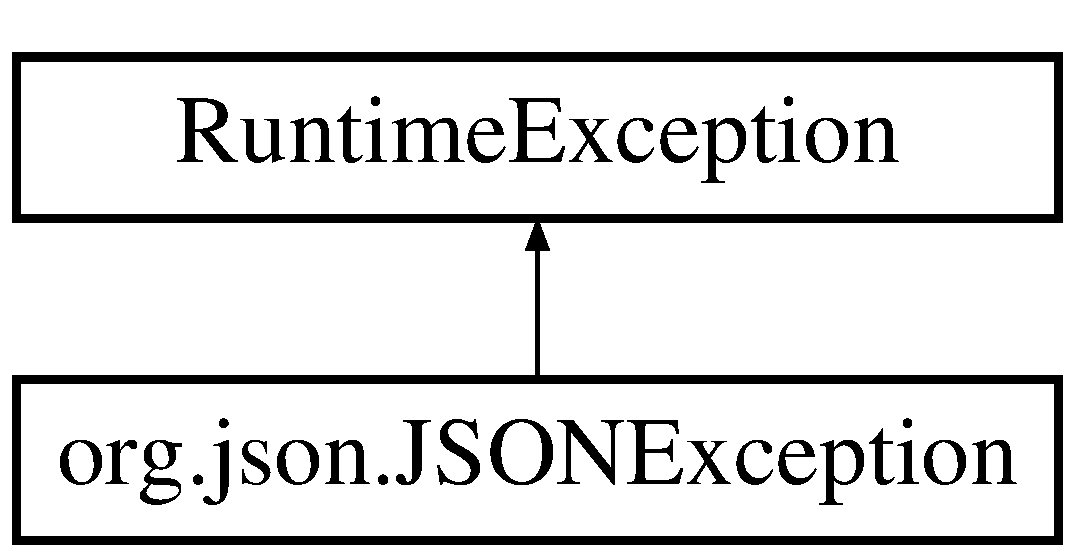
\includegraphics[height=2.000000cm]{classorg_1_1json_1_1_j_s_o_n_exception}
\end{center}
\end{figure}
\subsection*{Public Member Functions}
\begin{DoxyCompactItemize}
\item 
\hyperlink{classorg_1_1json_1_1_j_s_o_n_exception_a8251c83531dd05241eeddcd2eed31bae}{J\-S\-O\-N\-Exception} (String message)
\item 
\hyperlink{classorg_1_1json_1_1_j_s_o_n_exception_aa09b706ee690c9a2a4e96b93d64dff9b}{J\-S\-O\-N\-Exception} (Throwable \hyperlink{classorg_1_1json_1_1_j_s_o_n_exception_adfaad5c0b7a1d41430d2d1e701520e2b}{cause})
\item 
Throwable \hyperlink{classorg_1_1json_1_1_j_s_o_n_exception_a3215d707756f45b63a71728aebf7b918}{get\-Cause} ()
\end{DoxyCompactItemize}
\subsection*{Private Attributes}
\begin{DoxyCompactItemize}
\item 
Throwable \hyperlink{classorg_1_1json_1_1_j_s_o_n_exception_adfaad5c0b7a1d41430d2d1e701520e2b}{cause}
\end{DoxyCompactItemize}
\subsection*{Static Private Attributes}
\begin{DoxyCompactItemize}
\item 
static final long \hyperlink{classorg_1_1json_1_1_j_s_o_n_exception_afdd64d3f1a75f497c8641f02a49201c9}{serial\-Version\-U\-I\-D} = 0
\end{DoxyCompactItemize}


\subsection{Detailed Description}
The \hyperlink{classorg_1_1json_1_1_j_s_o_n_exception}{J\-S\-O\-N\-Exception} is thrown by the J\-S\-O\-N.\-org classes when things are amiss.

\begin{DoxyAuthor}{Author}
J\-S\-O\-N.\-org 
\end{DoxyAuthor}
\begin{DoxyVersion}{Version}
2013-\/02-\/10 
\end{DoxyVersion}


Definition at line 9 of file J\-S\-O\-N\-Exception.\-java.



\subsection{Constructor \& Destructor Documentation}
\hypertarget{classorg_1_1json_1_1_j_s_o_n_exception_a8251c83531dd05241eeddcd2eed31bae}{\index{org\-::json\-::\-J\-S\-O\-N\-Exception@{org\-::json\-::\-J\-S\-O\-N\-Exception}!J\-S\-O\-N\-Exception@{J\-S\-O\-N\-Exception}}
\index{J\-S\-O\-N\-Exception@{J\-S\-O\-N\-Exception}!org::json::JSONException@{org\-::json\-::\-J\-S\-O\-N\-Exception}}
\subsubsection[{J\-S\-O\-N\-Exception}]{\setlength{\rightskip}{0pt plus 5cm}org.\-json.\-J\-S\-O\-N\-Exception.\-J\-S\-O\-N\-Exception (
\begin{DoxyParamCaption}
\item[{String}]{message}
\end{DoxyParamCaption}
)}}\label{classorg_1_1json_1_1_j_s_o_n_exception_a8251c83531dd05241eeddcd2eed31bae}
Constructs a \hyperlink{classorg_1_1json_1_1_j_s_o_n_exception}{J\-S\-O\-N\-Exception} with an explanatory message.


\begin{DoxyParams}{Parameters}
{\em message} & Detail about the reason for the exception. \\
\hline
\end{DoxyParams}


Definition at line 19 of file J\-S\-O\-N\-Exception.\-java.


\begin{DoxyCode}
19                                          \{
20         super(message);
21     \}
\end{DoxyCode}
\hypertarget{classorg_1_1json_1_1_j_s_o_n_exception_aa09b706ee690c9a2a4e96b93d64dff9b}{\index{org\-::json\-::\-J\-S\-O\-N\-Exception@{org\-::json\-::\-J\-S\-O\-N\-Exception}!J\-S\-O\-N\-Exception@{J\-S\-O\-N\-Exception}}
\index{J\-S\-O\-N\-Exception@{J\-S\-O\-N\-Exception}!org::json::JSONException@{org\-::json\-::\-J\-S\-O\-N\-Exception}}
\subsubsection[{J\-S\-O\-N\-Exception}]{\setlength{\rightskip}{0pt plus 5cm}org.\-json.\-J\-S\-O\-N\-Exception.\-J\-S\-O\-N\-Exception (
\begin{DoxyParamCaption}
\item[{Throwable}]{cause}
\end{DoxyParamCaption}
)}}\label{classorg_1_1json_1_1_j_s_o_n_exception_aa09b706ee690c9a2a4e96b93d64dff9b}
Constructs a new \hyperlink{classorg_1_1json_1_1_j_s_o_n_exception}{J\-S\-O\-N\-Exception} with the specified cause. 

Definition at line 26 of file J\-S\-O\-N\-Exception.\-java.



References org.\-json.\-J\-S\-O\-N\-Exception.\-cause.


\begin{DoxyCode}
26                                           \{
27         super(\hyperlink{classorg_1_1json_1_1_j_s_o_n_exception_adfaad5c0b7a1d41430d2d1e701520e2b}{cause}.getMessage());
28         this.\hyperlink{classorg_1_1json_1_1_j_s_o_n_exception_adfaad5c0b7a1d41430d2d1e701520e2b}{cause} = \hyperlink{classorg_1_1json_1_1_j_s_o_n_exception_adfaad5c0b7a1d41430d2d1e701520e2b}{cause};
29     \}
\end{DoxyCode}


\subsection{Member Function Documentation}
\hypertarget{classorg_1_1json_1_1_j_s_o_n_exception_a3215d707756f45b63a71728aebf7b918}{\index{org\-::json\-::\-J\-S\-O\-N\-Exception@{org\-::json\-::\-J\-S\-O\-N\-Exception}!get\-Cause@{get\-Cause}}
\index{get\-Cause@{get\-Cause}!org::json::JSONException@{org\-::json\-::\-J\-S\-O\-N\-Exception}}
\subsubsection[{get\-Cause}]{\setlength{\rightskip}{0pt plus 5cm}Throwable org.\-json.\-J\-S\-O\-N\-Exception.\-get\-Cause (
\begin{DoxyParamCaption}
{}
\end{DoxyParamCaption}
)}}\label{classorg_1_1json_1_1_j_s_o_n_exception_a3215d707756f45b63a71728aebf7b918}
Returns the cause of this exception or null if the cause is nonexistent or unknown.

\begin{DoxyReturn}{Returns}
the cause of this exception or null if the cause is nonexistent or unknown. 
\end{DoxyReturn}


Definition at line 38 of file J\-S\-O\-N\-Exception.\-java.



References org.\-json.\-J\-S\-O\-N\-Exception.\-cause.


\begin{DoxyCode}
38                                 \{
39         \textcolor{keywordflow}{return} this.\hyperlink{classorg_1_1json_1_1_j_s_o_n_exception_adfaad5c0b7a1d41430d2d1e701520e2b}{cause};
40     \}
\end{DoxyCode}


\subsection{Member Data Documentation}
\hypertarget{classorg_1_1json_1_1_j_s_o_n_exception_adfaad5c0b7a1d41430d2d1e701520e2b}{\index{org\-::json\-::\-J\-S\-O\-N\-Exception@{org\-::json\-::\-J\-S\-O\-N\-Exception}!cause@{cause}}
\index{cause@{cause}!org::json::JSONException@{org\-::json\-::\-J\-S\-O\-N\-Exception}}
\subsubsection[{cause}]{\setlength{\rightskip}{0pt plus 5cm}Throwable org.\-json.\-J\-S\-O\-N\-Exception.\-cause\hspace{0.3cm}{\ttfamily [private]}}}\label{classorg_1_1json_1_1_j_s_o_n_exception_adfaad5c0b7a1d41430d2d1e701520e2b}


Definition at line 11 of file J\-S\-O\-N\-Exception.\-java.



Referenced by org.\-json.\-J\-S\-O\-N\-Exception.\-get\-Cause(), and org.\-json.\-J\-S\-O\-N\-Exception.\-J\-S\-O\-N\-Exception().

\hypertarget{classorg_1_1json_1_1_j_s_o_n_exception_afdd64d3f1a75f497c8641f02a49201c9}{\index{org\-::json\-::\-J\-S\-O\-N\-Exception@{org\-::json\-::\-J\-S\-O\-N\-Exception}!serial\-Version\-U\-I\-D@{serial\-Version\-U\-I\-D}}
\index{serial\-Version\-U\-I\-D@{serial\-Version\-U\-I\-D}!org::json::JSONException@{org\-::json\-::\-J\-S\-O\-N\-Exception}}
\subsubsection[{serial\-Version\-U\-I\-D}]{\setlength{\rightskip}{0pt plus 5cm}final long org.\-json.\-J\-S\-O\-N\-Exception.\-serial\-Version\-U\-I\-D = 0\hspace{0.3cm}{\ttfamily [static]}, {\ttfamily [private]}}}\label{classorg_1_1json_1_1_j_s_o_n_exception_afdd64d3f1a75f497c8641f02a49201c9}


Definition at line 10 of file J\-S\-O\-N\-Exception.\-java.



The documentation for this class was generated from the following file\-:\begin{DoxyCompactItemize}
\item 
org/json/\hyperlink{_j_s_o_n_exception_8java}{J\-S\-O\-N\-Exception.\-java}\end{DoxyCompactItemize}

\hypertarget{classorg_1_1json_1_1_j_s_o_n_m_l}{\section{org.\-json.\-J\-S\-O\-N\-M\-L Class Reference}
\label{classorg_1_1json_1_1_j_s_o_n_m_l}\index{org.\-json.\-J\-S\-O\-N\-M\-L@{org.\-json.\-J\-S\-O\-N\-M\-L}}
}
\subsection*{Static Public Member Functions}
\begin{DoxyCompactItemize}
\item 
static \hyperlink{classorg_1_1json_1_1_j_s_o_n_array}{J\-S\-O\-N\-Array} \hyperlink{classorg_1_1json_1_1_j_s_o_n_m_l_a97e622e1f610e21ba5cbd3167d4fb5a1}{to\-J\-S\-O\-N\-Array} (String string)  throws J\-S\-O\-N\-Exception 
\item 
static \hyperlink{classorg_1_1json_1_1_j_s_o_n_array}{J\-S\-O\-N\-Array} \hyperlink{classorg_1_1json_1_1_j_s_o_n_m_l_a82cc8221f4feee054e12a5689a2186f4}{to\-J\-S\-O\-N\-Array} (\hyperlink{classorg_1_1json_1_1_x_m_l_tokener}{X\-M\-L\-Tokener} x)  throws J\-S\-O\-N\-Exception 
\item 
static \hyperlink{classorg_1_1json_1_1_j_s_o_n_object}{J\-S\-O\-N\-Object} \hyperlink{classorg_1_1json_1_1_j_s_o_n_m_l_a9075449699e2ebca8721a6bdf04ee35f}{to\-J\-S\-O\-N\-Object} (\hyperlink{classorg_1_1json_1_1_x_m_l_tokener}{X\-M\-L\-Tokener} x)  throws J\-S\-O\-N\-Exception 
\item 
static \hyperlink{classorg_1_1json_1_1_j_s_o_n_object}{J\-S\-O\-N\-Object} \hyperlink{classorg_1_1json_1_1_j_s_o_n_m_l_aa517a2c5f1930ae22619425098e55f41}{to\-J\-S\-O\-N\-Object} (String string)  throws J\-S\-O\-N\-Exception 
\item 
static String \hyperlink{classorg_1_1json_1_1_j_s_o_n_m_l_aeb4921c45210936fbcd3a527e1df88fd}{to\-String} (\hyperlink{classorg_1_1json_1_1_j_s_o_n_array}{J\-S\-O\-N\-Array} ja)  throws J\-S\-O\-N\-Exception 
\item 
static String \hyperlink{classorg_1_1json_1_1_j_s_o_n_m_l_aa436f0b8577f68314e12f23f803437c2}{to\-String} (\hyperlink{classorg_1_1json_1_1_j_s_o_n_object}{J\-S\-O\-N\-Object} jo)  throws J\-S\-O\-N\-Exception 
\end{DoxyCompactItemize}
\subsection*{Static Private Member Functions}
\begin{DoxyCompactItemize}
\item 
static Object \hyperlink{classorg_1_1json_1_1_j_s_o_n_m_l_a3c36aa36d0d65f7d3f5aef426750faec}{parse} (\hyperlink{classorg_1_1json_1_1_x_m_l_tokener}{X\-M\-L\-Tokener} x, boolean array\-Form, \hyperlink{classorg_1_1json_1_1_j_s_o_n_array}{J\-S\-O\-N\-Array} ja)  throws J\-S\-O\-N\-Exception 
\end{DoxyCompactItemize}


\subsection{Detailed Description}
This provides static methods to convert an \hyperlink{classorg_1_1json_1_1_x_m_l}{X\-M\-L} text into a \hyperlink{classorg_1_1json_1_1_j_s_o_n_array}{J\-S\-O\-N\-Array} or \hyperlink{classorg_1_1json_1_1_j_s_o_n_object}{J\-S\-O\-N\-Object}, and to covert a \hyperlink{classorg_1_1json_1_1_j_s_o_n_array}{J\-S\-O\-N\-Array} or \hyperlink{classorg_1_1json_1_1_j_s_o_n_object}{J\-S\-O\-N\-Object} into an \hyperlink{classorg_1_1json_1_1_x_m_l}{X\-M\-L} text using the Json\-M\-L transform.

\begin{DoxyAuthor}{Author}
J\-S\-O\-N.\-org 
\end{DoxyAuthor}
\begin{DoxyVersion}{Version}
2012-\/03-\/28 
\end{DoxyVersion}


Definition at line 38 of file J\-S\-O\-N\-M\-L.\-java.



\subsection{Member Function Documentation}
\hypertarget{classorg_1_1json_1_1_j_s_o_n_m_l_a3c36aa36d0d65f7d3f5aef426750faec}{\index{org\-::json\-::\-J\-S\-O\-N\-M\-L@{org\-::json\-::\-J\-S\-O\-N\-M\-L}!parse@{parse}}
\index{parse@{parse}!org::json::JSONML@{org\-::json\-::\-J\-S\-O\-N\-M\-L}}
\subsubsection[{parse}]{\setlength{\rightskip}{0pt plus 5cm}static Object org.\-json.\-J\-S\-O\-N\-M\-L.\-parse (
\begin{DoxyParamCaption}
\item[{{\bf X\-M\-L\-Tokener}}]{x, }
\item[{boolean}]{array\-Form, }
\item[{{\bf J\-S\-O\-N\-Array}}]{ja}
\end{DoxyParamCaption}
) throws {\bf J\-S\-O\-N\-Exception}\hspace{0.3cm}{\ttfamily [static]}, {\ttfamily [private]}}}\label{classorg_1_1json_1_1_j_s_o_n_m_l_a3c36aa36d0d65f7d3f5aef426750faec}
Parse \hyperlink{classorg_1_1json_1_1_x_m_l}{X\-M\-L} values and store them in a \hyperlink{classorg_1_1json_1_1_j_s_o_n_array}{J\-S\-O\-N\-Array}. 
\begin{DoxyParams}{Parameters}
{\em x} & The \hyperlink{classorg_1_1json_1_1_x_m_l_tokener}{X\-M\-L\-Tokener} containing the source string. \\
\hline
{\em array\-Form} & true if array form, false if object form. \\
\hline
{\em ja} & The \hyperlink{classorg_1_1json_1_1_j_s_o_n_array}{J\-S\-O\-N\-Array} that is containing the current tag or null if we are at the outermost level. \\
\hline
\end{DoxyParams}
\begin{DoxyReturn}{Returns}
A \hyperlink{classorg_1_1json_1_1_j_s_o_n_array}{J\-S\-O\-N\-Array} if the value is the outermost tag, otherwise null. 
\end{DoxyReturn}

\begin{DoxyExceptions}{Exceptions}
{\em \hyperlink{classorg_1_1json_1_1_j_s_o_n_exception}{J\-S\-O\-N\-Exception}} & \\
\hline
\end{DoxyExceptions}


Definition at line 49 of file J\-S\-O\-N\-M\-L.\-java.



References org.\-json.\-J\-S\-O\-N\-Object.\-accumulate(), org.\-json.\-X\-M\-L.\-B\-A\-N\-G, org.\-json.\-X\-M\-L.\-E\-Q, org.\-json.\-X\-M\-L.\-G\-T, org.\-json.\-J\-S\-O\-N\-Array.\-length(), org.\-json.\-J\-S\-O\-N\-Object.\-length(), org.\-json.\-X\-M\-L.\-L\-T, org.\-json.\-J\-S\-O\-N\-Array.\-put(), org.\-json.\-J\-S\-O\-N\-Object.\-put(), org.\-json.\-X\-M\-L.\-Q\-U\-E\-S\-T, org.\-json.\-X\-M\-L.\-S\-L\-A\-S\-H, and org.\-json.\-X\-M\-L.\-string\-To\-Value().



Referenced by org.\-json.\-J\-S\-O\-N\-M\-L.\-to\-J\-S\-O\-N\-Array(), and org.\-json.\-J\-S\-O\-N\-M\-L.\-to\-J\-S\-O\-N\-Object().


\begin{DoxyCode}
53                            \{
54         String     attribute;
55         \textcolor{keywordtype}{char}       c;
56         String       closeTag = null;
57         \textcolor{keywordtype}{int}        i;
58         JSONArray  newja = null;
59         JSONObject newjo = null;
60         Object     token;
61         String       tagName = null;
62 
63 \textcolor{comment}{// Test for and skip past these forms:}
64 \textcolor{comment}{//      <!-- ... -->}
65 \textcolor{comment}{//      <![  ... ]]>}
66 \textcolor{comment}{//      <!   ...   >}
67 \textcolor{comment}{//      <?   ...  ?>}
68 
69         \textcolor{keywordflow}{while} (\textcolor{keyword}{true}) \{
70             \textcolor{keywordflow}{if} (!x.more()) \{
71                 \textcolor{keywordflow}{throw} x.syntaxError(\textcolor{stringliteral}{"Bad XML"});
72             \}
73             token = x.nextContent();
74             \textcolor{keywordflow}{if} (token == XML.LT) \{
75                 token = x.nextToken();
76                 \textcolor{keywordflow}{if} (token instanceof Character) \{
77                     \textcolor{keywordflow}{if} (token == XML.SLASH) \{
78 
79 \textcolor{comment}{// Close tag </}
80 
81                         token = x.nextToken();
82                         \textcolor{keywordflow}{if} (!(token instanceof String)) \{
83                             \textcolor{keywordflow}{throw} \textcolor{keyword}{new} JSONException(
84                                     \textcolor{stringliteral}{"Expected a closing name instead of '"} +
85                                     token + \textcolor{stringliteral}{"'."});
86                         \}
87                         \textcolor{keywordflow}{if} (x.nextToken() != XML.GT) \{
88                             \textcolor{keywordflow}{throw} x.syntaxError(\textcolor{stringliteral}{"Misshaped close tag"});
89                         \}
90                         \textcolor{keywordflow}{return} token;
91                     \} \textcolor{keywordflow}{else} \textcolor{keywordflow}{if} (token == XML.BANG) \{
92 
93 \textcolor{comment}{// <!}
94 
95                         c = x.next();
96                         \textcolor{keywordflow}{if} (c == \textcolor{charliteral}{'-'}) \{
97                             \textcolor{keywordflow}{if} (x.next() == \textcolor{charliteral}{'-'}) \{
98                                 x.skipPast(\textcolor{stringliteral}{"-->"});
99                             \} \textcolor{keywordflow}{else} \{
100                                 x.back();
101                             \}
102                         \} \textcolor{keywordflow}{else} \textcolor{keywordflow}{if} (c == \textcolor{charliteral}{'['}) \{
103                             token = x.nextToken();
104                             \textcolor{keywordflow}{if} (token.equals(\textcolor{stringliteral}{"CDATA"}) && x.next() == \textcolor{charliteral}{'['}) \{
105                                 \textcolor{keywordflow}{if} (ja != null) \{
106                                     ja.put(x.nextCDATA());
107                                 \}
108                             \} \textcolor{keywordflow}{else} \{
109                                 \textcolor{keywordflow}{throw} x.syntaxError(\textcolor{stringliteral}{"Expected 'CDATA['"});
110                             \}
111                         \} \textcolor{keywordflow}{else} \{
112                             i = 1;
113                             \textcolor{keywordflow}{do} \{
114                                 token = x.nextMeta();
115                                 \textcolor{keywordflow}{if} (token == null) \{
116                                     \textcolor{keywordflow}{throw} x.syntaxError(\textcolor{stringliteral}{"Missing '>' after '<!'."});
117                                 \} \textcolor{keywordflow}{else} \textcolor{keywordflow}{if} (token == XML.LT) \{
118                                     i += 1;
119                                 \} \textcolor{keywordflow}{else} \textcolor{keywordflow}{if} (token == XML.GT) \{
120                                     i -= 1;
121                                 \}
122                             \} \textcolor{keywordflow}{while} (i > 0);
123                         \}
124                     \} \textcolor{keywordflow}{else} \textcolor{keywordflow}{if} (token == XML.QUEST) \{
125 
126 \textcolor{comment}{// <?}
127 
128                         x.skipPast(\textcolor{stringliteral}{"?>"});
129                     \} \textcolor{keywordflow}{else} \{
130                         \textcolor{keywordflow}{throw} x.syntaxError(\textcolor{stringliteral}{"Misshaped tag"});
131                     \}
132 
133 \textcolor{comment}{// Open tag <}
134 
135                 \} \textcolor{keywordflow}{else} \{
136                     \textcolor{keywordflow}{if} (!(token instanceof String)) \{
137                         \textcolor{keywordflow}{throw} x.syntaxError(\textcolor{stringliteral}{"Bad tagName '"} + token + \textcolor{stringliteral}{"'."});
138                     \}
139                     tagName = (String)token;
140                     newja = \textcolor{keyword}{new} JSONArray();
141                     newjo = \textcolor{keyword}{new} JSONObject();
142                     \textcolor{keywordflow}{if} (arrayForm) \{
143                         newja.put(tagName);
144                         \textcolor{keywordflow}{if} (ja != null) \{
145                             ja.put(newja);
146                         \}
147                     \} \textcolor{keywordflow}{else} \{
148                         newjo.put(\textcolor{stringliteral}{"tagName"}, tagName);
149                         \textcolor{keywordflow}{if} (ja != null) \{
150                             ja.put(newjo);
151                         \}
152                     \}
153                     token = null;
154                     \textcolor{keywordflow}{for} (;;) \{
155                         \textcolor{keywordflow}{if} (token == null) \{
156                             token = x.nextToken();
157                         \}
158                         \textcolor{keywordflow}{if} (token == null) \{
159                             \textcolor{keywordflow}{throw} x.syntaxError(\textcolor{stringliteral}{"Misshaped tag"});
160                         \}
161                         \textcolor{keywordflow}{if} (!(token instanceof String)) \{
162                             \textcolor{keywordflow}{break};
163                         \}
164 
165 \textcolor{comment}{// attribute = value}
166 
167                         attribute = (String)token;
168                         \textcolor{keywordflow}{if} (!arrayForm && (\textcolor{stringliteral}{"tagName"}.equals(attribute) || \textcolor{stringliteral}{"childNode"}.equals(attribute))) \{
169                             \textcolor{keywordflow}{throw} x.syntaxError(\textcolor{stringliteral}{"Reserved attribute."});
170                         \}
171                         token = x.nextToken();
172                         \textcolor{keywordflow}{if} (token == XML.EQ) \{
173                             token = x.nextToken();
174                             \textcolor{keywordflow}{if} (!(token instanceof String)) \{
175                                 \textcolor{keywordflow}{throw} x.syntaxError(\textcolor{stringliteral}{"Missing value"});
176                             \}
177                             newjo.accumulate(attribute, XML.stringToValue((String)token));
178                             token = null;
179                         \} \textcolor{keywordflow}{else} \{
180                             newjo.accumulate(attribute, \textcolor{stringliteral}{""});
181                         \}
182                     \}
183                     \textcolor{keywordflow}{if} (arrayForm && newjo.length() > 0) \{
184                         newja.put(newjo);
185                     \}
186 
187 \textcolor{comment}{// Empty tag <.../>}
188 
189                     \textcolor{keywordflow}{if} (token == XML.SLASH) \{
190                         \textcolor{keywordflow}{if} (x.nextToken() != XML.GT) \{
191                             \textcolor{keywordflow}{throw} x.syntaxError(\textcolor{stringliteral}{"Misshaped tag"});
192                         \}
193                         \textcolor{keywordflow}{if} (ja == null) \{
194                             \textcolor{keywordflow}{if} (arrayForm) \{
195                                 \textcolor{keywordflow}{return} newja;
196                             \} \textcolor{keywordflow}{else} \{
197                                 \textcolor{keywordflow}{return} newjo;
198                             \}
199                         \}
200 
201 \textcolor{comment}{// Content, between <...> and </...>}
202 
203                     \} \textcolor{keywordflow}{else} \{
204                         \textcolor{keywordflow}{if} (token != XML.GT) \{
205                             \textcolor{keywordflow}{throw} x.syntaxError(\textcolor{stringliteral}{"Misshaped tag"});
206                         \}
207                         closeTag = (String)\hyperlink{classorg_1_1json_1_1_j_s_o_n_m_l_a3c36aa36d0d65f7d3f5aef426750faec}{parse}(x, arrayForm, newja);
208                         \textcolor{keywordflow}{if} (closeTag != null) \{
209                             \textcolor{keywordflow}{if} (!closeTag.equals(tagName)) \{
210                                 \textcolor{keywordflow}{throw} x.syntaxError(\textcolor{stringliteral}{"Mismatched '"} + tagName +
211                                         \textcolor{stringliteral}{"' and '"} + closeTag + \textcolor{stringliteral}{"'"});
212                             \}
213                             tagName = null;
214                             \textcolor{keywordflow}{if} (!arrayForm && newja.length() > 0) \{
215                                 newjo.put(\textcolor{stringliteral}{"childNodes"}, newja);
216                             \}
217                             \textcolor{keywordflow}{if} (ja == null) \{
218                                 \textcolor{keywordflow}{if} (arrayForm) \{
219                                     \textcolor{keywordflow}{return} newja;
220                                 \} \textcolor{keywordflow}{else} \{
221                                     \textcolor{keywordflow}{return} newjo;
222                                 \}
223                             \}
224                         \}
225                     \}
226                 \}
227             \} \textcolor{keywordflow}{else} \{
228                 \textcolor{keywordflow}{if} (ja != null) \{
229                     ja.put(token instanceof String
230                         ? XML.stringToValue((String)token)
231                         : token);
232                 \}
233             \}
234         \}
235     \}
\end{DoxyCode}
\hypertarget{classorg_1_1json_1_1_j_s_o_n_m_l_a97e622e1f610e21ba5cbd3167d4fb5a1}{\index{org\-::json\-::\-J\-S\-O\-N\-M\-L@{org\-::json\-::\-J\-S\-O\-N\-M\-L}!to\-J\-S\-O\-N\-Array@{to\-J\-S\-O\-N\-Array}}
\index{to\-J\-S\-O\-N\-Array@{to\-J\-S\-O\-N\-Array}!org::json::JSONML@{org\-::json\-::\-J\-S\-O\-N\-M\-L}}
\subsubsection[{to\-J\-S\-O\-N\-Array}]{\setlength{\rightskip}{0pt plus 5cm}static {\bf J\-S\-O\-N\-Array} org.\-json.\-J\-S\-O\-N\-M\-L.\-to\-J\-S\-O\-N\-Array (
\begin{DoxyParamCaption}
\item[{String}]{string}
\end{DoxyParamCaption}
) throws {\bf J\-S\-O\-N\-Exception}\hspace{0.3cm}{\ttfamily [static]}}}\label{classorg_1_1json_1_1_j_s_o_n_m_l_a97e622e1f610e21ba5cbd3167d4fb5a1}
Convert a well-\/formed (but not necessarily valid) \hyperlink{classorg_1_1json_1_1_x_m_l}{X\-M\-L} string into a \hyperlink{classorg_1_1json_1_1_j_s_o_n_array}{J\-S\-O\-N\-Array} using the Json\-M\-L transform. Each \hyperlink{classorg_1_1json_1_1_x_m_l}{X\-M\-L} tag is represented as a \hyperlink{classorg_1_1json_1_1_j_s_o_n_array}{J\-S\-O\-N\-Array} in which the first element is the tag name. If the tag has attributes, then the second element will be \hyperlink{classorg_1_1json_1_1_j_s_o_n_object}{J\-S\-O\-N\-Object} containing the name/value pairs. If the tag contains children, then strings and J\-S\-O\-N\-Arrays will represent the child tags. Comments, prologs, D\-T\-Ds, and {\ttfamily $<$\mbox{[} \mbox{[} \mbox{]}\mbox{]}$>$} are ignored. 
\begin{DoxyParams}{Parameters}
{\em string} & The source string. \\
\hline
\end{DoxyParams}
\begin{DoxyReturn}{Returns}
A \hyperlink{classorg_1_1json_1_1_j_s_o_n_array}{J\-S\-O\-N\-Array} containing the structured data from the \hyperlink{classorg_1_1json_1_1_x_m_l}{X\-M\-L} string. 
\end{DoxyReturn}

\begin{DoxyExceptions}{Exceptions}
{\em \hyperlink{classorg_1_1json_1_1_j_s_o_n_exception}{J\-S\-O\-N\-Exception}} & \\
\hline
\end{DoxyExceptions}


Definition at line 250 of file J\-S\-O\-N\-M\-L.\-java.


\begin{DoxyCode}
250                                                                             \{
251         \textcolor{keywordflow}{return} \hyperlink{classorg_1_1json_1_1_j_s_o_n_m_l_a97e622e1f610e21ba5cbd3167d4fb5a1}{toJSONArray}(\textcolor{keyword}{new} XMLTokener(\textcolor{keywordtype}{string}));
252     \}
\end{DoxyCode}
\hypertarget{classorg_1_1json_1_1_j_s_o_n_m_l_a82cc8221f4feee054e12a5689a2186f4}{\index{org\-::json\-::\-J\-S\-O\-N\-M\-L@{org\-::json\-::\-J\-S\-O\-N\-M\-L}!to\-J\-S\-O\-N\-Array@{to\-J\-S\-O\-N\-Array}}
\index{to\-J\-S\-O\-N\-Array@{to\-J\-S\-O\-N\-Array}!org::json::JSONML@{org\-::json\-::\-J\-S\-O\-N\-M\-L}}
\subsubsection[{to\-J\-S\-O\-N\-Array}]{\setlength{\rightskip}{0pt plus 5cm}static {\bf J\-S\-O\-N\-Array} org.\-json.\-J\-S\-O\-N\-M\-L.\-to\-J\-S\-O\-N\-Array (
\begin{DoxyParamCaption}
\item[{{\bf X\-M\-L\-Tokener}}]{x}
\end{DoxyParamCaption}
) throws {\bf J\-S\-O\-N\-Exception}\hspace{0.3cm}{\ttfamily [static]}}}\label{classorg_1_1json_1_1_j_s_o_n_m_l_a82cc8221f4feee054e12a5689a2186f4}
Convert a well-\/formed (but not necessarily valid) \hyperlink{classorg_1_1json_1_1_x_m_l}{X\-M\-L} string into a \hyperlink{classorg_1_1json_1_1_j_s_o_n_array}{J\-S\-O\-N\-Array} using the Json\-M\-L transform. Each \hyperlink{classorg_1_1json_1_1_x_m_l}{X\-M\-L} tag is represented as a \hyperlink{classorg_1_1json_1_1_j_s_o_n_array}{J\-S\-O\-N\-Array} in which the first element is the tag name. If the tag has attributes, then the second element will be \hyperlink{classorg_1_1json_1_1_j_s_o_n_object}{J\-S\-O\-N\-Object} containing the name/value pairs. If the tag contains children, then strings and J\-S\-O\-N\-Arrays will represent the child content and tags. Comments, prologs, D\-T\-Ds, and {\ttfamily $<$\mbox{[} \mbox{[} \mbox{]}\mbox{]}$>$} are ignored. 
\begin{DoxyParams}{Parameters}
{\em x} & An \hyperlink{classorg_1_1json_1_1_x_m_l_tokener}{X\-M\-L\-Tokener}. \\
\hline
\end{DoxyParams}
\begin{DoxyReturn}{Returns}
A \hyperlink{classorg_1_1json_1_1_j_s_o_n_array}{J\-S\-O\-N\-Array} containing the structured data from the \hyperlink{classorg_1_1json_1_1_x_m_l}{X\-M\-L} string. 
\end{DoxyReturn}

\begin{DoxyExceptions}{Exceptions}
{\em \hyperlink{classorg_1_1json_1_1_j_s_o_n_exception}{J\-S\-O\-N\-Exception}} & \\
\hline
\end{DoxyExceptions}


Definition at line 267 of file J\-S\-O\-N\-M\-L.\-java.



References org.\-json.\-J\-S\-O\-N\-M\-L.\-parse().


\begin{DoxyCode}
267                                                                            \{
268         \textcolor{keywordflow}{return} (JSONArray)\hyperlink{classorg_1_1json_1_1_j_s_o_n_m_l_a3c36aa36d0d65f7d3f5aef426750faec}{parse}(x, \textcolor{keyword}{true}, null);
269     \}
\end{DoxyCode}
\hypertarget{classorg_1_1json_1_1_j_s_o_n_m_l_a9075449699e2ebca8721a6bdf04ee35f}{\index{org\-::json\-::\-J\-S\-O\-N\-M\-L@{org\-::json\-::\-J\-S\-O\-N\-M\-L}!to\-J\-S\-O\-N\-Object@{to\-J\-S\-O\-N\-Object}}
\index{to\-J\-S\-O\-N\-Object@{to\-J\-S\-O\-N\-Object}!org::json::JSONML@{org\-::json\-::\-J\-S\-O\-N\-M\-L}}
\subsubsection[{to\-J\-S\-O\-N\-Object}]{\setlength{\rightskip}{0pt plus 5cm}static {\bf J\-S\-O\-N\-Object} org.\-json.\-J\-S\-O\-N\-M\-L.\-to\-J\-S\-O\-N\-Object (
\begin{DoxyParamCaption}
\item[{{\bf X\-M\-L\-Tokener}}]{x}
\end{DoxyParamCaption}
) throws {\bf J\-S\-O\-N\-Exception}\hspace{0.3cm}{\ttfamily [static]}}}\label{classorg_1_1json_1_1_j_s_o_n_m_l_a9075449699e2ebca8721a6bdf04ee35f}
Convert a well-\/formed (but not necessarily valid) \hyperlink{classorg_1_1json_1_1_x_m_l}{X\-M\-L} string into a \hyperlink{classorg_1_1json_1_1_j_s_o_n_object}{J\-S\-O\-N\-Object} using the Json\-M\-L transform. Each \hyperlink{classorg_1_1json_1_1_x_m_l}{X\-M\-L} tag is represented as a \hyperlink{classorg_1_1json_1_1_j_s_o_n_object}{J\-S\-O\-N\-Object} with a \char`\"{}tag\-Name\char`\"{} property. If the tag has attributes, then the attributes will be in the \hyperlink{classorg_1_1json_1_1_j_s_o_n_object}{J\-S\-O\-N\-Object} as properties. If the tag contains children, the object will have a \char`\"{}child\-Nodes\char`\"{} property which will be an array of strings and Json\-M\-L J\-S\-O\-N\-Objects.

Comments, prologs, D\-T\-Ds, and {\ttfamily $<$\mbox{[} \mbox{[} \mbox{]}\mbox{]}$>$} are ignored. 
\begin{DoxyParams}{Parameters}
{\em x} & An \hyperlink{classorg_1_1json_1_1_x_m_l_tokener}{X\-M\-L\-Tokener} of the \hyperlink{classorg_1_1json_1_1_x_m_l}{X\-M\-L} source text. \\
\hline
\end{DoxyParams}
\begin{DoxyReturn}{Returns}
A \hyperlink{classorg_1_1json_1_1_j_s_o_n_object}{J\-S\-O\-N\-Object} containing the structured data from the \hyperlink{classorg_1_1json_1_1_x_m_l}{X\-M\-L} string. 
\end{DoxyReturn}

\begin{DoxyExceptions}{Exceptions}
{\em \hyperlink{classorg_1_1json_1_1_j_s_o_n_exception}{J\-S\-O\-N\-Exception}} & \\
\hline
\end{DoxyExceptions}


Definition at line 285 of file J\-S\-O\-N\-M\-L.\-java.



References org.\-json.\-J\-S\-O\-N\-M\-L.\-parse().



Referenced by org.\-json.\-J\-S\-O\-N\-M\-L.\-to\-J\-S\-O\-N\-Object().


\begin{DoxyCode}
285                                                                              \{
286            \textcolor{keywordflow}{return} (JSONObject)\hyperlink{classorg_1_1json_1_1_j_s_o_n_m_l_a3c36aa36d0d65f7d3f5aef426750faec}{parse}(x, \textcolor{keyword}{false}, null);
287     \}
\end{DoxyCode}
\hypertarget{classorg_1_1json_1_1_j_s_o_n_m_l_aa517a2c5f1930ae22619425098e55f41}{\index{org\-::json\-::\-J\-S\-O\-N\-M\-L@{org\-::json\-::\-J\-S\-O\-N\-M\-L}!to\-J\-S\-O\-N\-Object@{to\-J\-S\-O\-N\-Object}}
\index{to\-J\-S\-O\-N\-Object@{to\-J\-S\-O\-N\-Object}!org::json::JSONML@{org\-::json\-::\-J\-S\-O\-N\-M\-L}}
\subsubsection[{to\-J\-S\-O\-N\-Object}]{\setlength{\rightskip}{0pt plus 5cm}static {\bf J\-S\-O\-N\-Object} org.\-json.\-J\-S\-O\-N\-M\-L.\-to\-J\-S\-O\-N\-Object (
\begin{DoxyParamCaption}
\item[{String}]{string}
\end{DoxyParamCaption}
) throws {\bf J\-S\-O\-N\-Exception}\hspace{0.3cm}{\ttfamily [static]}}}\label{classorg_1_1json_1_1_j_s_o_n_m_l_aa517a2c5f1930ae22619425098e55f41}
Convert a well-\/formed (but not necessarily valid) \hyperlink{classorg_1_1json_1_1_x_m_l}{X\-M\-L} string into a \hyperlink{classorg_1_1json_1_1_j_s_o_n_object}{J\-S\-O\-N\-Object} using the Json\-M\-L transform. Each \hyperlink{classorg_1_1json_1_1_x_m_l}{X\-M\-L} tag is represented as a \hyperlink{classorg_1_1json_1_1_j_s_o_n_object}{J\-S\-O\-N\-Object} with a \char`\"{}tag\-Name\char`\"{} property. If the tag has attributes, then the attributes will be in the \hyperlink{classorg_1_1json_1_1_j_s_o_n_object}{J\-S\-O\-N\-Object} as properties. If the tag contains children, the object will have a \char`\"{}child\-Nodes\char`\"{} property which will be an array of strings and Json\-M\-L J\-S\-O\-N\-Objects.

Comments, prologs, D\-T\-Ds, and {\ttfamily $<$\mbox{[} \mbox{[} \mbox{]}\mbox{]}$>$} are ignored. 
\begin{DoxyParams}{Parameters}
{\em string} & The \hyperlink{classorg_1_1json_1_1_x_m_l}{X\-M\-L} source text. \\
\hline
\end{DoxyParams}
\begin{DoxyReturn}{Returns}
A \hyperlink{classorg_1_1json_1_1_j_s_o_n_object}{J\-S\-O\-N\-Object} containing the structured data from the \hyperlink{classorg_1_1json_1_1_x_m_l}{X\-M\-L} string. 
\end{DoxyReturn}

\begin{DoxyExceptions}{Exceptions}
{\em \hyperlink{classorg_1_1json_1_1_j_s_o_n_exception}{J\-S\-O\-N\-Exception}} & \\
\hline
\end{DoxyExceptions}


Definition at line 303 of file J\-S\-O\-N\-M\-L.\-java.



References org.\-json.\-J\-S\-O\-N\-M\-L.\-to\-J\-S\-O\-N\-Object().


\begin{DoxyCode}
303                                                                               \{
304         \textcolor{keywordflow}{return} \hyperlink{classorg_1_1json_1_1_j_s_o_n_m_l_a9075449699e2ebca8721a6bdf04ee35f}{toJSONObject}(\textcolor{keyword}{new} XMLTokener(\textcolor{keywordtype}{string}));
305     \}
\end{DoxyCode}
\hypertarget{classorg_1_1json_1_1_j_s_o_n_m_l_aeb4921c45210936fbcd3a527e1df88fd}{\index{org\-::json\-::\-J\-S\-O\-N\-M\-L@{org\-::json\-::\-J\-S\-O\-N\-M\-L}!to\-String@{to\-String}}
\index{to\-String@{to\-String}!org::json::JSONML@{org\-::json\-::\-J\-S\-O\-N\-M\-L}}
\subsubsection[{to\-String}]{\setlength{\rightskip}{0pt plus 5cm}static String org.\-json.\-J\-S\-O\-N\-M\-L.\-to\-String (
\begin{DoxyParamCaption}
\item[{{\bf J\-S\-O\-N\-Array}}]{ja}
\end{DoxyParamCaption}
) throws {\bf J\-S\-O\-N\-Exception}\hspace{0.3cm}{\ttfamily [static]}}}\label{classorg_1_1json_1_1_j_s_o_n_m_l_aeb4921c45210936fbcd3a527e1df88fd}
Reverse the \hyperlink{classorg_1_1json_1_1_j_s_o_n_m_l}{J\-S\-O\-N\-M\-L} transformation, making an \hyperlink{classorg_1_1json_1_1_x_m_l}{X\-M\-L} text from a \hyperlink{classorg_1_1json_1_1_j_s_o_n_array}{J\-S\-O\-N\-Array}. 
\begin{DoxyParams}{Parameters}
{\em ja} & A \hyperlink{classorg_1_1json_1_1_j_s_o_n_array}{J\-S\-O\-N\-Array}. \\
\hline
\end{DoxyParams}
\begin{DoxyReturn}{Returns}
An \hyperlink{classorg_1_1json_1_1_x_m_l}{X\-M\-L} string. 
\end{DoxyReturn}

\begin{DoxyExceptions}{Exceptions}
{\em \hyperlink{classorg_1_1json_1_1_j_s_o_n_exception}{J\-S\-O\-N\-Exception}} & \\
\hline
\end{DoxyExceptions}


Definition at line 314 of file J\-S\-O\-N\-M\-L.\-java.



References org.\-json.\-X\-M\-L.\-escape(), org.\-json.\-J\-S\-O\-N\-Object.\-keys(), org.\-json.\-X\-M\-L.\-no\-Space(), and org.\-json.\-J\-S\-O\-N\-Object.\-opt\-String().



Referenced by org.\-json.\-J\-S\-O\-N\-M\-L.\-to\-String().


\begin{DoxyCode}
314                                                                      \{
315         \textcolor{keywordtype}{int}             i;
316         JSONObject   jo;
317         String       key;
318         Iterator     keys;
319         \textcolor{keywordtype}{int}             length;
320         Object         object;
321         StringBuffer sb = \textcolor{keyword}{new} StringBuffer();
322         String       tagName;
323         String       value;
324 
325 \textcolor{comment}{// Emit <tagName}
326 
327         tagName = ja.getString(0);
328         XML.noSpace(tagName);
329         tagName = XML.escape(tagName);
330         sb.append(\textcolor{charliteral}{'<'});
331         sb.append(tagName);
332 
333         \textcolor{keywordtype}{object} = ja.opt(1);
334         \textcolor{keywordflow}{if} (\textcolor{keywordtype}{object} instanceof JSONObject) \{
335             i = 2;
336             jo = (JSONObject)\textcolor{keywordtype}{object};
337 
338 \textcolor{comment}{// Emit the attributes}
339 
340             keys = jo.keys();
341             \textcolor{keywordflow}{while} (keys.hasNext()) \{
342                 key = keys.next().toString();
343                 XML.noSpace(key);
344                 value = jo.optString(key);
345                 \textcolor{keywordflow}{if} (value != null) \{
346                     sb.append(\textcolor{charliteral}{' '});
347                     sb.append(XML.escape(key));
348                     sb.append(\textcolor{charliteral}{'='});
349                     sb.append(\textcolor{charliteral}{'"'});
350                     sb.append(XML.escape(value));
351                     sb.append(\textcolor{charliteral}{'"'});
352                 \}
353             \}
354         \} \textcolor{keywordflow}{else} \{
355             i = 1;
356         \}
357 
358 \textcolor{comment}{//Emit content in body}
359 
360         length = ja.length();
361         \textcolor{keywordflow}{if} (i >= length) \{
362             sb.append(\textcolor{charliteral}{'/'});
363             sb.append(\textcolor{charliteral}{'>'});
364         \} \textcolor{keywordflow}{else} \{
365             sb.append(\textcolor{charliteral}{'>'});
366             \textcolor{keywordflow}{do} \{
367                 \textcolor{keywordtype}{object} = ja.get(i);
368                 i += 1;
369                 \textcolor{keywordflow}{if} (\textcolor{keywordtype}{object} != null) \{
370                     \textcolor{keywordflow}{if} (\textcolor{keywordtype}{object} instanceof String) \{
371                         sb.append(XML.escape(\textcolor{keywordtype}{object}.toString()));
372                     \} \textcolor{keywordflow}{else} \textcolor{keywordflow}{if} (\textcolor{keywordtype}{object} instanceof JSONObject) \{
373                         sb.append(\hyperlink{classorg_1_1json_1_1_j_s_o_n_m_l_aeb4921c45210936fbcd3a527e1df88fd}{toString}((JSONObject)\textcolor{keywordtype}{object}));
374                     \} \textcolor{keywordflow}{else} \textcolor{keywordflow}{if} (\textcolor{keywordtype}{object} instanceof JSONArray) \{
375                         sb.append(\hyperlink{classorg_1_1json_1_1_j_s_o_n_m_l_aeb4921c45210936fbcd3a527e1df88fd}{toString}((JSONArray)\textcolor{keywordtype}{object}));
376                     \}
377                 \}
378             \} \textcolor{keywordflow}{while} (i < length);
379             sb.append(\textcolor{charliteral}{'<'});
380             sb.append(\textcolor{charliteral}{'/'});
381             sb.append(tagName);
382             sb.append(\textcolor{charliteral}{'>'});
383         \}
384         \textcolor{keywordflow}{return} sb.toString();
385     \}
\end{DoxyCode}
\hypertarget{classorg_1_1json_1_1_j_s_o_n_m_l_aa436f0b8577f68314e12f23f803437c2}{\index{org\-::json\-::\-J\-S\-O\-N\-M\-L@{org\-::json\-::\-J\-S\-O\-N\-M\-L}!to\-String@{to\-String}}
\index{to\-String@{to\-String}!org::json::JSONML@{org\-::json\-::\-J\-S\-O\-N\-M\-L}}
\subsubsection[{to\-String}]{\setlength{\rightskip}{0pt plus 5cm}static String org.\-json.\-J\-S\-O\-N\-M\-L.\-to\-String (
\begin{DoxyParamCaption}
\item[{{\bf J\-S\-O\-N\-Object}}]{jo}
\end{DoxyParamCaption}
) throws {\bf J\-S\-O\-N\-Exception}\hspace{0.3cm}{\ttfamily [static]}}}\label{classorg_1_1json_1_1_j_s_o_n_m_l_aa436f0b8577f68314e12f23f803437c2}
Reverse the \hyperlink{classorg_1_1json_1_1_j_s_o_n_m_l}{J\-S\-O\-N\-M\-L} transformation, making an \hyperlink{classorg_1_1json_1_1_x_m_l}{X\-M\-L} text from a \hyperlink{classorg_1_1json_1_1_j_s_o_n_object}{J\-S\-O\-N\-Object}. The \hyperlink{classorg_1_1json_1_1_j_s_o_n_object}{J\-S\-O\-N\-Object} must contain a \char`\"{}tag\-Name\char`\"{} property. If it has children, then it must have a \char`\"{}child\-Nodes\char`\"{} property containing an array of objects. The other properties are attributes with string values. 
\begin{DoxyParams}{Parameters}
{\em jo} & A \hyperlink{classorg_1_1json_1_1_j_s_o_n_object}{J\-S\-O\-N\-Object}. \\
\hline
\end{DoxyParams}
\begin{DoxyReturn}{Returns}
An \hyperlink{classorg_1_1json_1_1_x_m_l}{X\-M\-L} string. 
\end{DoxyReturn}

\begin{DoxyExceptions}{Exceptions}
{\em \hyperlink{classorg_1_1json_1_1_j_s_o_n_exception}{J\-S\-O\-N\-Exception}} & \\
\hline
\end{DoxyExceptions}


Definition at line 396 of file J\-S\-O\-N\-M\-L.\-java.



References org.\-json.\-X\-M\-L.\-escape(), org.\-json.\-J\-S\-O\-N\-Array.\-get(), org.\-json.\-J\-S\-O\-N\-Array.\-length(), org.\-json.\-X\-M\-L.\-no\-Space(), org.\-json.\-J\-S\-O\-N\-Array.\-opt\-J\-S\-O\-N\-Array(), org.\-json.\-J\-S\-O\-N\-Array.\-opt\-String(), and org.\-json.\-J\-S\-O\-N\-M\-L.\-to\-String().


\begin{DoxyCode}
396                                                                       \{
397         StringBuffer sb = \textcolor{keyword}{new} StringBuffer();
398         \textcolor{keywordtype}{int}          i;
399         JSONArray    ja;
400         String       key;
401         Iterator     keys;
402         \textcolor{keywordtype}{int}          length;
403         Object         object;
404         String       tagName;
405         String       value;
406 
407 \textcolor{comment}{//Emit <tagName}
408 
409         tagName = jo.optString(\textcolor{stringliteral}{"tagName"});
410         \textcolor{keywordflow}{if} (tagName == null) \{
411             \textcolor{keywordflow}{return} XML.escape(jo.toString());
412         \}
413         XML.noSpace(tagName);
414         tagName = XML.escape(tagName);
415         sb.append(\textcolor{charliteral}{'<'});
416         sb.append(tagName);
417 
418 \textcolor{comment}{//Emit the attributes}
419 
420         keys = jo.keys();
421         \textcolor{keywordflow}{while} (keys.hasNext()) \{
422             key = keys.next().toString();
423             \textcolor{keywordflow}{if} (!\textcolor{stringliteral}{"tagName"}.equals(key) && !\textcolor{stringliteral}{"childNodes"}.equals(key)) \{
424                 XML.noSpace(key);
425                 value = jo.optString(key);
426                 \textcolor{keywordflow}{if} (value != null) \{
427                     sb.append(\textcolor{charliteral}{' '});
428                     sb.append(XML.escape(key));
429                     sb.append(\textcolor{charliteral}{'='});
430                     sb.append(\textcolor{charliteral}{'"'});
431                     sb.append(XML.escape(value));
432                     sb.append(\textcolor{charliteral}{'"'});
433                 \}
434             \}
435         \}
436 
437 \textcolor{comment}{//Emit content in body}
438 
439         ja = jo.optJSONArray(\textcolor{stringliteral}{"childNodes"});
440         \textcolor{keywordflow}{if} (ja == null) \{
441             sb.append(\textcolor{charliteral}{'/'});
442             sb.append(\textcolor{charliteral}{'>'});
443         \} \textcolor{keywordflow}{else} \{
444             sb.append(\textcolor{charliteral}{'>'});
445             length = ja.length();
446             \textcolor{keywordflow}{for} (i = 0; i < length; i += 1) \{
447                 \textcolor{keywordtype}{object} = ja.get(i);
448                 \textcolor{keywordflow}{if} (\textcolor{keywordtype}{object} != null) \{
449                     \textcolor{keywordflow}{if} (\textcolor{keywordtype}{object} instanceof String) \{
450                         sb.append(XML.escape(\textcolor{keywordtype}{object}.toString()));
451                     \} \textcolor{keywordflow}{else} \textcolor{keywordflow}{if} (\textcolor{keywordtype}{object} instanceof JSONObject) \{
452                         sb.append(\hyperlink{classorg_1_1json_1_1_j_s_o_n_m_l_aeb4921c45210936fbcd3a527e1df88fd}{toString}((JSONObject)\textcolor{keywordtype}{object}));
453                     \} \textcolor{keywordflow}{else} \textcolor{keywordflow}{if} (\textcolor{keywordtype}{object} instanceof JSONArray) \{
454                         sb.append(\hyperlink{classorg_1_1json_1_1_j_s_o_n_m_l_aeb4921c45210936fbcd3a527e1df88fd}{toString}((JSONArray)\textcolor{keywordtype}{object}));
455                     \} \textcolor{keywordflow}{else} \{
456                         sb.append(\textcolor{keywordtype}{object}.\hyperlink{classorg_1_1json_1_1_j_s_o_n_m_l_aeb4921c45210936fbcd3a527e1df88fd}{toString}());
457                     \}
458                 \}
459             \}
460             sb.append(\textcolor{charliteral}{'<'});
461             sb.append(\textcolor{charliteral}{'/'});
462             sb.append(tagName);
463             sb.append(\textcolor{charliteral}{'>'});
464         \}
465         \textcolor{keywordflow}{return} sb.toString();
466     \}
\end{DoxyCode}


The documentation for this class was generated from the following file\-:\begin{DoxyCompactItemize}
\item 
org/json/\hyperlink{_j_s_o_n_m_l_8java}{J\-S\-O\-N\-M\-L.\-java}\end{DoxyCompactItemize}

\hypertarget{classorg_1_1json_1_1_j_s_o_n_object}{\section{org.\-json.\-J\-S\-O\-N\-Object Class Reference}
\label{classorg_1_1json_1_1_j_s_o_n_object}\index{org.\-json.\-J\-S\-O\-N\-Object@{org.\-json.\-J\-S\-O\-N\-Object}}
}
\subsection*{Classes}
\begin{DoxyCompactItemize}
\item 
class \hyperlink{classorg_1_1json_1_1_j_s_o_n_object_1_1_null}{Null}
\end{DoxyCompactItemize}
\subsection*{Public Member Functions}
\begin{DoxyCompactItemize}
\item 
\hyperlink{classorg_1_1json_1_1_j_s_o_n_object_a7c17e59daff74ce50c6677c6f5da233d}{J\-S\-O\-N\-Object} ()
\item 
\hyperlink{classorg_1_1json_1_1_j_s_o_n_object_a0e61a2a56e4a34ac5c8730497c320fe9}{J\-S\-O\-N\-Object} (\hyperlink{classorg_1_1json_1_1_j_s_o_n_object}{J\-S\-O\-N\-Object} jo, String\mbox{[}$\,$\mbox{]} \hyperlink{classorg_1_1json_1_1_j_s_o_n_object_a02e83de70e290231527d1760c4dd30fc}{names})
\item 
\hyperlink{classorg_1_1json_1_1_j_s_o_n_object_a30954f996711f48cb2dc9b456824e02e}{J\-S\-O\-N\-Object} (\hyperlink{classorg_1_1json_1_1_j_s_o_n_tokener}{J\-S\-O\-N\-Tokener} x)  throws J\-S\-O\-N\-Exception 
\item 
\hyperlink{classorg_1_1json_1_1_j_s_o_n_object_ac17536c9315efb5a42a741deac16c2bf}{J\-S\-O\-N\-Object} (Map \hyperlink{classorg_1_1json_1_1_j_s_o_n_object_a88de444c62dae3f3193d1276bb87ba31}{map})
\item 
\hyperlink{classorg_1_1json_1_1_j_s_o_n_object_adf96cd2952efa10c86156b9c8f4fe9b1}{J\-S\-O\-N\-Object} (Object bean)
\item 
\hyperlink{classorg_1_1json_1_1_j_s_o_n_object_af3f343eaf2cca8718a55d0f105807f9b}{J\-S\-O\-N\-Object} (Object object, String \hyperlink{classorg_1_1json_1_1_j_s_o_n_object_a02e83de70e290231527d1760c4dd30fc}{names}\mbox{[}$\,$\mbox{]})
\item 
\hyperlink{classorg_1_1json_1_1_j_s_o_n_object_a015b17aea42a3c1762b66cd1c0803d04}{J\-S\-O\-N\-Object} (String source)  throws J\-S\-O\-N\-Exception 
\item 
\hyperlink{classorg_1_1json_1_1_j_s_o_n_object_a8c9f78e54c6e38ecb786fee7163e26fa}{J\-S\-O\-N\-Object} (String base\-Name, Locale locale)  throws J\-S\-O\-N\-Exception 
\item 
\hyperlink{classorg_1_1json_1_1_j_s_o_n_object}{J\-S\-O\-N\-Object} \hyperlink{classorg_1_1json_1_1_j_s_o_n_object_a2c8b90ffd10c970175d63daf3e682634}{accumulate} (String key, Object value)  throws J\-S\-O\-N\-Exception 
\item 
\hyperlink{classorg_1_1json_1_1_j_s_o_n_object}{J\-S\-O\-N\-Object} \hyperlink{classorg_1_1json_1_1_j_s_o_n_object_ae6f06b948080a76425a818ebcfb2c001}{append} (String key, Object value)  throws J\-S\-O\-N\-Exception 
\item 
Object \hyperlink{classorg_1_1json_1_1_j_s_o_n_object_ac98329762a354373a0d3fddc2855dd61}{get} (String key)  throws J\-S\-O\-N\-Exception 
\item 
boolean \hyperlink{classorg_1_1json_1_1_j_s_o_n_object_ab40aab8de47233591ac4ad9d1b31adc0}{get\-Boolean} (String key)  throws J\-S\-O\-N\-Exception 
\item 
double \hyperlink{classorg_1_1json_1_1_j_s_o_n_object_abeec5fe03f3a260b7ec7a2b3076ca5ec}{get\-Double} (String key)  throws J\-S\-O\-N\-Exception 
\item 
int \hyperlink{classorg_1_1json_1_1_j_s_o_n_object_a3756c60c7c7bfecbdde3c3b5b1bcf385}{get\-Int} (String key)  throws J\-S\-O\-N\-Exception 
\item 
\hyperlink{classorg_1_1json_1_1_j_s_o_n_array}{J\-S\-O\-N\-Array} \hyperlink{classorg_1_1json_1_1_j_s_o_n_object_a884ee44fe958e9ea737d6c5e1180cb62}{get\-J\-S\-O\-N\-Array} (String key)  throws J\-S\-O\-N\-Exception 
\item 
\hyperlink{classorg_1_1json_1_1_j_s_o_n_object}{J\-S\-O\-N\-Object} \hyperlink{classorg_1_1json_1_1_j_s_o_n_object_a6011679cb15a3aac5944bb4a8af9f7fb}{get\-J\-S\-O\-N\-Object} (String key)  throws J\-S\-O\-N\-Exception 
\item 
long \hyperlink{classorg_1_1json_1_1_j_s_o_n_object_a3547552ed2f4c5d415eab8202e8d6158}{get\-Long} (String key)  throws J\-S\-O\-N\-Exception 
\item 
String \hyperlink{classorg_1_1json_1_1_j_s_o_n_object_a7140df2bac96f4d75a3f338ed16d1212}{get\-String} (String key)  throws J\-S\-O\-N\-Exception 
\item 
boolean \hyperlink{classorg_1_1json_1_1_j_s_o_n_object_aa3d594c3e7a5b6d9b89aa6cda03bac28}{has} (String key)
\item 
\hyperlink{classorg_1_1json_1_1_j_s_o_n_object}{J\-S\-O\-N\-Object} \hyperlink{classorg_1_1json_1_1_j_s_o_n_object_a4c808cfee4389ecf543781feaa1b950c}{increment} (String key)  throws J\-S\-O\-N\-Exception 
\item 
boolean \hyperlink{classorg_1_1json_1_1_j_s_o_n_object_a8de41c5807522df5a7b888a0ffd6b69b}{is\-Null} (String key)
\item 
Iterator \hyperlink{classorg_1_1json_1_1_j_s_o_n_object_a1909c454712287d3a7c988beaa0613ff}{keys} ()
\item 
Set \hyperlink{classorg_1_1json_1_1_j_s_o_n_object_a60a1757ce5acba415364ba982f7e48b2}{key\-Set} ()
\item 
int \hyperlink{classorg_1_1json_1_1_j_s_o_n_object_a2c47910737728e063a8395d3a9152d42}{length} ()
\item 
\hyperlink{classorg_1_1json_1_1_j_s_o_n_array}{J\-S\-O\-N\-Array} \hyperlink{classorg_1_1json_1_1_j_s_o_n_object_a02e83de70e290231527d1760c4dd30fc}{names} ()
\item 
Object \hyperlink{classorg_1_1json_1_1_j_s_o_n_object_a51eeabb3fde00474d3ffd7381ad5d311}{opt} (String key)
\item 
boolean \hyperlink{classorg_1_1json_1_1_j_s_o_n_object_ae2fd84f0e465ade590e47ba7bdce683b}{opt\-Boolean} (String key)
\item 
boolean \hyperlink{classorg_1_1json_1_1_j_s_o_n_object_ae46a66bde2bc443b63ed93cb26677e34}{opt\-Boolean} (String key, boolean default\-Value)
\item 
double \hyperlink{classorg_1_1json_1_1_j_s_o_n_object_a69bf1cb7de87f4b196c0081ddc4c6f58}{opt\-Double} (String key)
\item 
double \hyperlink{classorg_1_1json_1_1_j_s_o_n_object_ab5c3964b0ef382a85927000e743f8281}{opt\-Double} (String key, double default\-Value)
\item 
int \hyperlink{classorg_1_1json_1_1_j_s_o_n_object_abeb2c17bd5a09ab51b25e4b330983a97}{opt\-Int} (String key)
\item 
int \hyperlink{classorg_1_1json_1_1_j_s_o_n_object_a80567fb28cd07b9d5148d7610605305e}{opt\-Int} (String key, int default\-Value)
\item 
\hyperlink{classorg_1_1json_1_1_j_s_o_n_array}{J\-S\-O\-N\-Array} \hyperlink{classorg_1_1json_1_1_j_s_o_n_object_a1e0dce653705a1df438636fbb4fe94e2}{opt\-J\-S\-O\-N\-Array} (String key)
\item 
\hyperlink{classorg_1_1json_1_1_j_s_o_n_object}{J\-S\-O\-N\-Object} \hyperlink{classorg_1_1json_1_1_j_s_o_n_object_aa1024c804613178b09532ef7549e7b2b}{opt\-J\-S\-O\-N\-Object} (String key)
\item 
long \hyperlink{classorg_1_1json_1_1_j_s_o_n_object_af37dbbf760c1833402c986a62c4baef8}{opt\-Long} (String key)
\item 
long \hyperlink{classorg_1_1json_1_1_j_s_o_n_object_aa826ad7537ebfac8adda13f53ee0008b}{opt\-Long} (String key, long default\-Value)
\item 
String \hyperlink{classorg_1_1json_1_1_j_s_o_n_object_afee65e7bb15356d0fa9006ef391449e0}{opt\-String} (String key)
\item 
String \hyperlink{classorg_1_1json_1_1_j_s_o_n_object_a6501a2a9b5a97560d74337c082a32732}{opt\-String} (String key, String default\-Value)
\item 
\hyperlink{classorg_1_1json_1_1_j_s_o_n_object}{J\-S\-O\-N\-Object} \hyperlink{classorg_1_1json_1_1_j_s_o_n_object_a92b8b4edda8b4805abca24f5b689748b}{put} (String key, boolean value)  throws J\-S\-O\-N\-Exception 
\item 
\hyperlink{classorg_1_1json_1_1_j_s_o_n_object}{J\-S\-O\-N\-Object} \hyperlink{classorg_1_1json_1_1_j_s_o_n_object_ac5829feb500547a73f7ba1d0a090b9dc}{put} (String key, Collection value)  throws J\-S\-O\-N\-Exception 
\item 
\hyperlink{classorg_1_1json_1_1_j_s_o_n_object}{J\-S\-O\-N\-Object} \hyperlink{classorg_1_1json_1_1_j_s_o_n_object_a669cae1e6dd7bcab4a55d4a7078a0e72}{put} (String key, double value)  throws J\-S\-O\-N\-Exception 
\item 
\hyperlink{classorg_1_1json_1_1_j_s_o_n_object}{J\-S\-O\-N\-Object} \hyperlink{classorg_1_1json_1_1_j_s_o_n_object_a36a08204331752dffedc6e9d1b6aa297}{put} (String key, int value)  throws J\-S\-O\-N\-Exception 
\item 
\hyperlink{classorg_1_1json_1_1_j_s_o_n_object}{J\-S\-O\-N\-Object} \hyperlink{classorg_1_1json_1_1_j_s_o_n_object_a5807cd038e9ae979a692db1b99461205}{put} (String key, long value)  throws J\-S\-O\-N\-Exception 
\item 
\hyperlink{classorg_1_1json_1_1_j_s_o_n_object}{J\-S\-O\-N\-Object} \hyperlink{classorg_1_1json_1_1_j_s_o_n_object_a31371313d65f4239673c3cb521489176}{put} (String key, Map value)  throws J\-S\-O\-N\-Exception 
\item 
\hyperlink{classorg_1_1json_1_1_j_s_o_n_object}{J\-S\-O\-N\-Object} \hyperlink{classorg_1_1json_1_1_j_s_o_n_object_a2af440c4653ad8a23b0ac5ded37cd4d5}{put} (String key, Object value)  throws J\-S\-O\-N\-Exception 
\item 
\hyperlink{classorg_1_1json_1_1_j_s_o_n_object}{J\-S\-O\-N\-Object} \hyperlink{classorg_1_1json_1_1_j_s_o_n_object_ac6cc7fe095a7711be90f2e02163ef49e}{put\-Once} (String key, Object value)  throws J\-S\-O\-N\-Exception 
\item 
\hyperlink{classorg_1_1json_1_1_j_s_o_n_object}{J\-S\-O\-N\-Object} \hyperlink{classorg_1_1json_1_1_j_s_o_n_object_a023672439a8c851a663a183120fc126e}{put\-Opt} (String key, Object value)  throws J\-S\-O\-N\-Exception 
\item 
Object \hyperlink{classorg_1_1json_1_1_j_s_o_n_object_af4faca830e4bb6a00bccad695bd58c4d}{remove} (String key)
\item 
\hyperlink{classorg_1_1json_1_1_j_s_o_n_array}{J\-S\-O\-N\-Array} \hyperlink{classorg_1_1json_1_1_j_s_o_n_object_acafa0ef1407022894738177b3195e9f3}{to\-J\-S\-O\-N\-Array} (\hyperlink{classorg_1_1json_1_1_j_s_o_n_array}{J\-S\-O\-N\-Array} \hyperlink{classorg_1_1json_1_1_j_s_o_n_object_a02e83de70e290231527d1760c4dd30fc}{names})  throws J\-S\-O\-N\-Exception 
\item 
String \hyperlink{classorg_1_1json_1_1_j_s_o_n_object_a7f8cab6eb354ceb416a421574b4be424}{to\-String} ()
\item 
String \hyperlink{classorg_1_1json_1_1_j_s_o_n_object_a56087516560b91c8aebbba67efda1a61}{to\-String} (int indent\-Factor)  throws J\-S\-O\-N\-Exception 
\item 
Writer \hyperlink{classorg_1_1json_1_1_j_s_o_n_object_ac810606f683376f15962ed9b32db9eba}{write} (Writer writer)  throws J\-S\-O\-N\-Exception 
\end{DoxyCompactItemize}
\subsection*{Static Public Member Functions}
\begin{DoxyCompactItemize}
\item 
static String \hyperlink{classorg_1_1json_1_1_j_s_o_n_object_aad3ea50c3546331486737bcb24e42460}{double\-To\-String} (double d)
\item 
static String\mbox{[}$\,$\mbox{]} \hyperlink{classorg_1_1json_1_1_j_s_o_n_object_a30d4e44e4c8e03341c346970a00ba283}{get\-Names} (\hyperlink{classorg_1_1json_1_1_j_s_o_n_object}{J\-S\-O\-N\-Object} jo)
\item 
static String\mbox{[}$\,$\mbox{]} \hyperlink{classorg_1_1json_1_1_j_s_o_n_object_acf2ec104b4cbbf2947b155d54047efe8}{get\-Names} (Object object)
\item 
static String \hyperlink{classorg_1_1json_1_1_j_s_o_n_object_a5ea1eb29e2e3bdc7b4fae0579ead8525}{number\-To\-String} (Number number)  throws J\-S\-O\-N\-Exception 
\item 
static String \hyperlink{classorg_1_1json_1_1_j_s_o_n_object_abe60222a3919d3f88f104486c1ef13fe}{quote} (String string)
\item 
static Writer \hyperlink{classorg_1_1json_1_1_j_s_o_n_object_aac3d22e558d472049d4c8702cdaf676a}{quote} (String string, Writer w)  throws I\-O\-Exception 
\item 
static Object \hyperlink{classorg_1_1json_1_1_j_s_o_n_object_a23f861897abe58eb41c044dd63667319}{string\-To\-Value} (String string)
\item 
static void \hyperlink{classorg_1_1json_1_1_j_s_o_n_object_a406920be130176bad74d605bae04a6da}{test\-Validity} (Object o)  throws J\-S\-O\-N\-Exception 
\item 
static String \hyperlink{classorg_1_1json_1_1_j_s_o_n_object_ab386b6f594205eecdbe023ad7cb26105}{value\-To\-String} (Object value)  throws J\-S\-O\-N\-Exception 
\item 
static Object \hyperlink{classorg_1_1json_1_1_j_s_o_n_object_a5aa793d5ebe4bb6002bd37d84d65742e}{wrap} (Object object)
\end{DoxyCompactItemize}
\subsection*{Static Public Attributes}
\begin{DoxyCompactItemize}
\item 
static final Object \hyperlink{classorg_1_1json_1_1_j_s_o_n_object_a01c74a31a1abfd34ab13beb9347855ac}{N\-U\-L\-L} = new \hyperlink{classorg_1_1json_1_1_j_s_o_n_object_1_1_null}{Null}()
\end{DoxyCompactItemize}
\subsection*{Package Functions}
\begin{DoxyCompactItemize}
\item 
Writer \hyperlink{classorg_1_1json_1_1_j_s_o_n_object_afccc699dd9731cbee68c4e3efa8f45c8}{write} (Writer writer, int indent\-Factor, int \hyperlink{classorg_1_1json_1_1_j_s_o_n_object_ade4aa5090d5636a0318db80ba32764be}{indent})  throws J\-S\-O\-N\-Exception 
\end{DoxyCompactItemize}
\subsection*{Static Package Functions}
\begin{DoxyCompactItemize}
\item 
static final Writer \hyperlink{classorg_1_1json_1_1_j_s_o_n_object_a45a696bfd8f909a5b7afcefb71ed6f58}{write\-Value} (Writer writer, Object value, int indent\-Factor, int \hyperlink{classorg_1_1json_1_1_j_s_o_n_object_ade4aa5090d5636a0318db80ba32764be}{indent})  throws J\-S\-O\-N\-Exception, I\-O\-Exception 
\item 
static final void \hyperlink{classorg_1_1json_1_1_j_s_o_n_object_ade4aa5090d5636a0318db80ba32764be}{indent} (Writer writer, int indent)  throws I\-O\-Exception 
\end{DoxyCompactItemize}
\subsection*{Private Member Functions}
\begin{DoxyCompactItemize}
\item 
void \hyperlink{classorg_1_1json_1_1_j_s_o_n_object_ac10eaec5716b5868f263b0d101a7e164}{populate\-Map} (Object bean)
\end{DoxyCompactItemize}
\subsection*{Private Attributes}
\begin{DoxyCompactItemize}
\item 
final Map \hyperlink{classorg_1_1json_1_1_j_s_o_n_object_a88de444c62dae3f3193d1276bb87ba31}{map}
\end{DoxyCompactItemize}
\subsection*{Static Private Attributes}
\begin{DoxyCompactItemize}
\item 
static final int \hyperlink{classorg_1_1json_1_1_j_s_o_n_object_a982bf3253548748e80d16b1783a22ccc}{key\-Pool\-Size} = 100
\item 
static Hash\-Map \hyperlink{classorg_1_1json_1_1_j_s_o_n_object_a7bcba855d8493d0205256068ddd41314}{key\-Pool} = new Hash\-Map(\hyperlink{classorg_1_1json_1_1_j_s_o_n_object_a982bf3253548748e80d16b1783a22ccc}{key\-Pool\-Size})
\end{DoxyCompactItemize}


\subsection{Detailed Description}
A \hyperlink{classorg_1_1json_1_1_j_s_o_n_object}{J\-S\-O\-N\-Object} is an unordered collection of name/value pairs. Its external form is a string wrapped in curly braces with colons between the names and values, and commas between the values and names. The internal form is an object having {\ttfamily get} and {\ttfamily opt} methods for accessing the values by name, and {\ttfamily put} methods for adding or replacing values by name. The values can be any of these types\-: {\ttfamily Boolean}, {\ttfamily \hyperlink{classorg_1_1json_1_1_j_s_o_n_array}{J\-S\-O\-N\-Array}}, {\ttfamily \hyperlink{classorg_1_1json_1_1_j_s_o_n_object}{J\-S\-O\-N\-Object}}, {\ttfamily Number}, {\ttfamily String}, or the {\ttfamily \hyperlink{classorg_1_1json_1_1_j_s_o_n_object_a01c74a31a1abfd34ab13beb9347855ac}{J\-S\-O\-N\-Object.\-N\-U\-L\-L}} object. A \hyperlink{classorg_1_1json_1_1_j_s_o_n_object}{J\-S\-O\-N\-Object} constructor can be used to convert an external form J\-S\-O\-N text into an internal form whose values can be retrieved with the {\ttfamily get} and {\ttfamily opt} methods, or to convert values into a J\-S\-O\-N text using the {\ttfamily put} and {\ttfamily to\-String} methods. A {\ttfamily get} method returns a value if one can be found, and throws an exception if one cannot be found. An {\ttfamily opt} method returns a default value instead of throwing an exception, and so is useful for obtaining optional values. 

The generic {\ttfamily \hyperlink{classorg_1_1json_1_1_j_s_o_n_object_ac98329762a354373a0d3fddc2855dd61}{get()}} and {\ttfamily \hyperlink{classorg_1_1json_1_1_j_s_o_n_object_a51eeabb3fde00474d3ffd7381ad5d311}{opt()}} methods return an object, which you can cast or query for type. There are also typed {\ttfamily get} and {\ttfamily opt} methods that do type checking and type coercion for you. The opt methods differ from the get methods in that they do not throw. Instead, they return a specified value, such as null. 

The {\ttfamily put} methods add or replace values in an object. For example,


\begin{DoxyPre}
myString = new \hyperlink{classorg_1_1json_1_1_j_s_o_n_object_a7c17e59daff74ce50c6677c6f5da233d}{JSONObject()}
        .put("JSON", "Hello, World!").\hyperlink{classorg_1_1json_1_1_j_s_o_n_object_a7f8cab6eb354ceb416a421574b4be424}{toString()};
\end{DoxyPre}


produces the string {\ttfamily \{\char`\"{}\-J\-S\-O\-N\char`\"{}\-: \char`\"{}\-Hello, World\char`\"{}\}}. 

The texts produced by the {\ttfamily to\-String} methods strictly conform to the J\-S\-O\-N syntax rules. The constructors are more forgiving in the texts they will accept\-: 
\begin{DoxyItemize}
\item An extra {\ttfamily ,}~
\footnotesize (comma)
\normalsize  may appear just before the closing brace. 
\item Strings may be quoted with {\ttfamily '}~
\footnotesize (single quote)
\normalsize . 
\item Strings do not need to be quoted at all if they do not begin with a quote or single quote, and if they do not contain leading or trailing spaces, and if they do not contain any of these characters\-: {\ttfamily \{ \} \mbox{[} \mbox{]} / \textbackslash{} \-: , \#} and if they do not look like numbers and if they are not the reserved words {\ttfamily true}, {\ttfamily false}, or {\ttfamily null}. 
\end{DoxyItemize}

\begin{DoxyAuthor}{Author}
J\-S\-O\-N.\-org 
\end{DoxyAuthor}
\begin{DoxyVersion}{Version}
2013-\/04-\/18 
\end{DoxyVersion}


Definition at line 95 of file J\-S\-O\-N\-Object.\-java.



\subsection{Constructor \& Destructor Documentation}
\hypertarget{classorg_1_1json_1_1_j_s_o_n_object_a7c17e59daff74ce50c6677c6f5da233d}{\index{org\-::json\-::\-J\-S\-O\-N\-Object@{org\-::json\-::\-J\-S\-O\-N\-Object}!J\-S\-O\-N\-Object@{J\-S\-O\-N\-Object}}
\index{J\-S\-O\-N\-Object@{J\-S\-O\-N\-Object}!org::json::JSONObject@{org\-::json\-::\-J\-S\-O\-N\-Object}}
\subsubsection[{J\-S\-O\-N\-Object}]{\setlength{\rightskip}{0pt plus 5cm}org.\-json.\-J\-S\-O\-N\-Object.\-J\-S\-O\-N\-Object (
\begin{DoxyParamCaption}
{}
\end{DoxyParamCaption}
)}}\label{classorg_1_1json_1_1_j_s_o_n_object_a7c17e59daff74ce50c6677c6f5da233d}
Construct an empty \hyperlink{classorg_1_1json_1_1_j_s_o_n_object}{J\-S\-O\-N\-Object}. 

Definition at line 164 of file J\-S\-O\-N\-Object.\-java.



References org.\-json.\-J\-S\-O\-N\-Object.\-map.



Referenced by org.\-json.\-J\-S\-O\-N\-Object.\-J\-S\-O\-N\-Object(), org.\-json.\-J\-S\-O\-N\-Object.\-opt\-J\-S\-O\-N\-Object(), org.\-json.\-J\-S\-O\-N\-Object.\-put(), org.\-json.\-J\-S\-O\-N\-Object.\-value\-To\-String(), org.\-json.\-J\-S\-O\-N\-Object.\-wrap(), and org.\-json.\-J\-S\-O\-N\-Object.\-write\-Value().


\begin{DoxyCode}
164                         \{
165         this.\hyperlink{classorg_1_1json_1_1_j_s_o_n_object_a88de444c62dae3f3193d1276bb87ba31}{map} = \textcolor{keyword}{new} HashMap();
166     \}
\end{DoxyCode}
\hypertarget{classorg_1_1json_1_1_j_s_o_n_object_a0e61a2a56e4a34ac5c8730497c320fe9}{\index{org\-::json\-::\-J\-S\-O\-N\-Object@{org\-::json\-::\-J\-S\-O\-N\-Object}!J\-S\-O\-N\-Object@{J\-S\-O\-N\-Object}}
\index{J\-S\-O\-N\-Object@{J\-S\-O\-N\-Object}!org::json::JSONObject@{org\-::json\-::\-J\-S\-O\-N\-Object}}
\subsubsection[{J\-S\-O\-N\-Object}]{\setlength{\rightskip}{0pt plus 5cm}org.\-json.\-J\-S\-O\-N\-Object.\-J\-S\-O\-N\-Object (
\begin{DoxyParamCaption}
\item[{{\bf J\-S\-O\-N\-Object}}]{jo, }
\item[{String\mbox{[}$\,$\mbox{]}}]{names}
\end{DoxyParamCaption}
)}}\label{classorg_1_1json_1_1_j_s_o_n_object_a0e61a2a56e4a34ac5c8730497c320fe9}
Construct a \hyperlink{classorg_1_1json_1_1_j_s_o_n_object}{J\-S\-O\-N\-Object} from a subset of another \hyperlink{classorg_1_1json_1_1_j_s_o_n_object}{J\-S\-O\-N\-Object}. An array of strings is used to identify the keys that should be copied. Missing keys are ignored.


\begin{DoxyParams}{Parameters}
{\em jo} & A \hyperlink{classorg_1_1json_1_1_j_s_o_n_object}{J\-S\-O\-N\-Object}. \\
\hline
{\em names} & An array of strings. \\
\hline
\end{DoxyParams}

\begin{DoxyExceptions}{Exceptions}
{\em \hyperlink{classorg_1_1json_1_1_j_s_o_n_exception}{J\-S\-O\-N\-Exception}} & \\
\hline
{\em \hyperlink{classorg_1_1json_1_1_j_s_o_n_exception}{J\-S\-O\-N\-Exception}} & If a value is a non-\/finite number or if a name is duplicated. \\
\hline
\end{DoxyExceptions}


Definition at line 182 of file J\-S\-O\-N\-Object.\-java.



References org.\-json.\-J\-S\-O\-N\-Object.\-opt(), and org.\-json.\-J\-S\-O\-N\-Object.\-put\-Once().


\begin{DoxyCode}
182                                                      \{
183         \textcolor{keyword}{this}();
184         \textcolor{keywordflow}{for} (\textcolor{keywordtype}{int} i = 0; i < \hyperlink{classorg_1_1json_1_1_j_s_o_n_object_a02e83de70e290231527d1760c4dd30fc}{names}.\hyperlink{classorg_1_1json_1_1_j_s_o_n_array_a8382a78090007f650a02895ecbf3c8ec}{length}; i += 1) \{
185             \textcolor{keywordflow}{try} \{
186                 this.\hyperlink{classorg_1_1json_1_1_j_s_o_n_object_ac6cc7fe095a7711be90f2e02163ef49e}{putOnce}(\hyperlink{classorg_1_1json_1_1_j_s_o_n_object_a02e83de70e290231527d1760c4dd30fc}{names}[i], jo.\hyperlink{classorg_1_1json_1_1_j_s_o_n_array_a19aa83c80cded3d0a252c212ceca7954}{opt}(\hyperlink{classorg_1_1json_1_1_j_s_o_n_object_a02e83de70e290231527d1760c4dd30fc}{names}[i]));
187             \} \textcolor{keywordflow}{catch} (Exception ignore) \{
188             \}
189         \}
190     \}
\end{DoxyCode}
\hypertarget{classorg_1_1json_1_1_j_s_o_n_object_a30954f996711f48cb2dc9b456824e02e}{\index{org\-::json\-::\-J\-S\-O\-N\-Object@{org\-::json\-::\-J\-S\-O\-N\-Object}!J\-S\-O\-N\-Object@{J\-S\-O\-N\-Object}}
\index{J\-S\-O\-N\-Object@{J\-S\-O\-N\-Object}!org::json::JSONObject@{org\-::json\-::\-J\-S\-O\-N\-Object}}
\subsubsection[{J\-S\-O\-N\-Object}]{\setlength{\rightskip}{0pt plus 5cm}org.\-json.\-J\-S\-O\-N\-Object.\-J\-S\-O\-N\-Object (
\begin{DoxyParamCaption}
\item[{{\bf J\-S\-O\-N\-Tokener}}]{x}
\end{DoxyParamCaption}
) throws {\bf J\-S\-O\-N\-Exception}}}\label{classorg_1_1json_1_1_j_s_o_n_object_a30954f996711f48cb2dc9b456824e02e}
Construct a \hyperlink{classorg_1_1json_1_1_j_s_o_n_object}{J\-S\-O\-N\-Object} from a \hyperlink{classorg_1_1json_1_1_j_s_o_n_tokener}{J\-S\-O\-N\-Tokener}.


\begin{DoxyParams}{Parameters}
{\em x} & A \hyperlink{classorg_1_1json_1_1_j_s_o_n_tokener}{J\-S\-O\-N\-Tokener} object containing the source string. \\
\hline
\end{DoxyParams}

\begin{DoxyExceptions}{Exceptions}
{\em \hyperlink{classorg_1_1json_1_1_j_s_o_n_exception}{J\-S\-O\-N\-Exception}} & If there is a syntax error in the source string or a duplicated key. \\
\hline
\end{DoxyExceptions}


Definition at line 201 of file J\-S\-O\-N\-Object.\-java.



References org.\-json.\-J\-S\-O\-N\-Object.\-put\-Once().


\begin{DoxyCode}
201                                                           \{
202         \textcolor{keyword}{this}();
203         \textcolor{keywordtype}{char} c;
204         String key;
205 
206         \textcolor{keywordflow}{if} (x.nextClean() != \textcolor{charliteral}{'\{'}) \{
207             \textcolor{keywordflow}{throw} x.syntaxError(\textcolor{stringliteral}{"A JSONObject text must begin with '\{'"});
208         \}
209         \textcolor{keywordflow}{for} (;;) \{
210             c = x.nextClean();
211             \textcolor{keywordflow}{switch} (c) \{
212             \textcolor{keywordflow}{case} 0:
213                 \textcolor{keywordflow}{throw} x.syntaxError(\textcolor{stringliteral}{"A JSONObject text must end with '\}'"});
214             \textcolor{keywordflow}{case} \textcolor{charliteral}{'\}'}:
215                 \textcolor{keywordflow}{return};
216             \textcolor{keywordflow}{default}:
217                 x.back();
218                 key = x.nextValue().toString();
219             \}
220 
221 \textcolor{comment}{// The key is followed by ':'.}
222 
223             c = x.nextClean();
224             \textcolor{keywordflow}{if} (c != \textcolor{charliteral}{':'}) \{
225                 \textcolor{keywordflow}{throw} x.syntaxError(\textcolor{stringliteral}{"Expected a ':' after a key"});
226             \}
227             this.\hyperlink{classorg_1_1json_1_1_j_s_o_n_object_ac6cc7fe095a7711be90f2e02163ef49e}{putOnce}(key, x.nextValue());
228 
229 \textcolor{comment}{// Pairs are separated by ','.}
230 
231             \textcolor{keywordflow}{switch} (x.nextClean()) \{
232             \textcolor{keywordflow}{case} \textcolor{charliteral}{';'}:
233             \textcolor{keywordflow}{case} \textcolor{charliteral}{','}:
234                 \textcolor{keywordflow}{if} (x.nextClean() == \textcolor{charliteral}{'\}'}) \{
235                     \textcolor{keywordflow}{return};
236                 \}
237                 x.back();
238                 \textcolor{keywordflow}{break};
239             \textcolor{keywordflow}{case} \textcolor{charliteral}{'\}'}:
240                 \textcolor{keywordflow}{return};
241             \textcolor{keywordflow}{default}:
242                 \textcolor{keywordflow}{throw} x.syntaxError(\textcolor{stringliteral}{"Expected a ',' or '\}'"});
243             \}
244         \}
245     \}
\end{DoxyCode}
\hypertarget{classorg_1_1json_1_1_j_s_o_n_object_ac17536c9315efb5a42a741deac16c2bf}{\index{org\-::json\-::\-J\-S\-O\-N\-Object@{org\-::json\-::\-J\-S\-O\-N\-Object}!J\-S\-O\-N\-Object@{J\-S\-O\-N\-Object}}
\index{J\-S\-O\-N\-Object@{J\-S\-O\-N\-Object}!org::json::JSONObject@{org\-::json\-::\-J\-S\-O\-N\-Object}}
\subsubsection[{J\-S\-O\-N\-Object}]{\setlength{\rightskip}{0pt plus 5cm}org.\-json.\-J\-S\-O\-N\-Object.\-J\-S\-O\-N\-Object (
\begin{DoxyParamCaption}
\item[{Map}]{map}
\end{DoxyParamCaption}
)}}\label{classorg_1_1json_1_1_j_s_o_n_object_ac17536c9315efb5a42a741deac16c2bf}
Construct a \hyperlink{classorg_1_1json_1_1_j_s_o_n_object}{J\-S\-O\-N\-Object} from a Map.


\begin{DoxyParams}{Parameters}
{\em map} & A map object that can be used to initialize the contents of the \hyperlink{classorg_1_1json_1_1_j_s_o_n_object}{J\-S\-O\-N\-Object}. \\
\hline
\end{DoxyParams}

\begin{DoxyExceptions}{Exceptions}
{\em \hyperlink{classorg_1_1json_1_1_j_s_o_n_exception}{J\-S\-O\-N\-Exception}} & \\
\hline
\end{DoxyExceptions}


Definition at line 255 of file J\-S\-O\-N\-Object.\-java.



References org.\-json.\-J\-S\-O\-N\-Object.\-wrap().


\begin{DoxyCode}
255                                \{
256         this.\hyperlink{classorg_1_1json_1_1_j_s_o_n_object_a88de444c62dae3f3193d1276bb87ba31}{map} = \textcolor{keyword}{new} HashMap();
257         \textcolor{keywordflow}{if} (\hyperlink{classorg_1_1json_1_1_j_s_o_n_object_a88de444c62dae3f3193d1276bb87ba31}{map} != null) \{
258             Iterator i = \hyperlink{classorg_1_1json_1_1_j_s_o_n_object_a88de444c62dae3f3193d1276bb87ba31}{map}.entrySet().iterator();
259             \textcolor{keywordflow}{while} (i.hasNext()) \{
260                 Map.Entry e = (Map.Entry) i.next();
261                 Object value = e.getValue();
262                 \textcolor{keywordflow}{if} (value != null) \{
263                     this.\hyperlink{classorg_1_1json_1_1_j_s_o_n_object_a88de444c62dae3f3193d1276bb87ba31}{map}.put(e.getKey(), \hyperlink{classorg_1_1json_1_1_j_s_o_n_object_a5aa793d5ebe4bb6002bd37d84d65742e}{wrap}(value));
264                 \}
265             \}
266         \}
267     \}
\end{DoxyCode}
\hypertarget{classorg_1_1json_1_1_j_s_o_n_object_adf96cd2952efa10c86156b9c8f4fe9b1}{\index{org\-::json\-::\-J\-S\-O\-N\-Object@{org\-::json\-::\-J\-S\-O\-N\-Object}!J\-S\-O\-N\-Object@{J\-S\-O\-N\-Object}}
\index{J\-S\-O\-N\-Object@{J\-S\-O\-N\-Object}!org::json::JSONObject@{org\-::json\-::\-J\-S\-O\-N\-Object}}
\subsubsection[{J\-S\-O\-N\-Object}]{\setlength{\rightskip}{0pt plus 5cm}org.\-json.\-J\-S\-O\-N\-Object.\-J\-S\-O\-N\-Object (
\begin{DoxyParamCaption}
\item[{Object}]{bean}
\end{DoxyParamCaption}
)}}\label{classorg_1_1json_1_1_j_s_o_n_object_adf96cd2952efa10c86156b9c8f4fe9b1}
Construct a \hyperlink{classorg_1_1json_1_1_j_s_o_n_object}{J\-S\-O\-N\-Object} from an Object using bean getters. It reflects on all of the public methods of the object. For each of the methods with no parameters and a name starting with {\ttfamily \char`\"{}get\char`\"{}} or {\ttfamily \char`\"{}is\char`\"{}} followed by an uppercase letter, the method is invoked, and a key and the value returned from the getter method are put into the new \hyperlink{classorg_1_1json_1_1_j_s_o_n_object}{J\-S\-O\-N\-Object}.

The key is formed by removing the {\ttfamily \char`\"{}get\char`\"{}} or {\ttfamily \char`\"{}is\char`\"{}} prefix. If the second remaining character is not upper case, then the first character is converted to lower case.

For example, if an object has a method named {\ttfamily \char`\"{}get\-Name\char`\"{}}, and if the result of calling {\ttfamily object.\-get\-Name()} is {\ttfamily \char`\"{}\-Larry Fine\char`\"{}}, then the \hyperlink{classorg_1_1json_1_1_j_s_o_n_object}{J\-S\-O\-N\-Object} will contain {\ttfamily \char`\"{}name\char`\"{}\-: \char`\"{}\-Larry Fine\char`\"{}}.


\begin{DoxyParams}{Parameters}
{\em bean} & An object that has getter methods that should be used to make a \hyperlink{classorg_1_1json_1_1_j_s_o_n_object}{J\-S\-O\-N\-Object}. \\
\hline
\end{DoxyParams}


Definition at line 290 of file J\-S\-O\-N\-Object.\-java.



References org.\-json.\-J\-S\-O\-N\-Object.\-populate\-Map().


\begin{DoxyCode}
290                                    \{
291         \textcolor{keyword}{this}();
292         this.\hyperlink{classorg_1_1json_1_1_j_s_o_n_object_ac10eaec5716b5868f263b0d101a7e164}{populateMap}(bean);
293     \}
\end{DoxyCode}
\hypertarget{classorg_1_1json_1_1_j_s_o_n_object_af3f343eaf2cca8718a55d0f105807f9b}{\index{org\-::json\-::\-J\-S\-O\-N\-Object@{org\-::json\-::\-J\-S\-O\-N\-Object}!J\-S\-O\-N\-Object@{J\-S\-O\-N\-Object}}
\index{J\-S\-O\-N\-Object@{J\-S\-O\-N\-Object}!org::json::JSONObject@{org\-::json\-::\-J\-S\-O\-N\-Object}}
\subsubsection[{J\-S\-O\-N\-Object}]{\setlength{\rightskip}{0pt plus 5cm}org.\-json.\-J\-S\-O\-N\-Object.\-J\-S\-O\-N\-Object (
\begin{DoxyParamCaption}
\item[{Object}]{object, }
\item[{String}]{names\mbox{[}$\,$\mbox{]}}
\end{DoxyParamCaption}
)}}\label{classorg_1_1json_1_1_j_s_o_n_object_af3f343eaf2cca8718a55d0f105807f9b}
Construct a \hyperlink{classorg_1_1json_1_1_j_s_o_n_object}{J\-S\-O\-N\-Object} from an Object, using reflection to find the public members. The resulting \hyperlink{classorg_1_1json_1_1_j_s_o_n_object}{J\-S\-O\-N\-Object}'s keys will be the strings from the names array, and the values will be the field values associated with those keys in the object. If a key is not found or not visible, then it will not be copied into the new \hyperlink{classorg_1_1json_1_1_j_s_o_n_object}{J\-S\-O\-N\-Object}.


\begin{DoxyParams}{Parameters}
{\em object} & An object that has fields that should be used to make a \hyperlink{classorg_1_1json_1_1_j_s_o_n_object}{J\-S\-O\-N\-Object}. \\
\hline
{\em names} & An array of strings, the names of the fields to be obtained from the object. \\
\hline
\end{DoxyParams}


Definition at line 309 of file J\-S\-O\-N\-Object.\-java.



References org.\-json.\-J\-S\-O\-N\-Object.\-put\-Opt().


\begin{DoxyCode}
309                                                      \{
310         \textcolor{keyword}{this}();
311         Class c = \textcolor{keywordtype}{object}.getClass();
312         \textcolor{keywordflow}{for} (\textcolor{keywordtype}{int} i = 0; i < \hyperlink{classorg_1_1json_1_1_j_s_o_n_object_a02e83de70e290231527d1760c4dd30fc}{names}.\hyperlink{classorg_1_1json_1_1_j_s_o_n_array_a8382a78090007f650a02895ecbf3c8ec}{length}; i += 1) \{
313             String name = \hyperlink{classorg_1_1json_1_1_j_s_o_n_object_a02e83de70e290231527d1760c4dd30fc}{names}[i];
314             \textcolor{keywordflow}{try} \{
315                 this.\hyperlink{classorg_1_1json_1_1_j_s_o_n_object_a023672439a8c851a663a183120fc126e}{putOpt}(name, c.getField(name).get(\textcolor{keywordtype}{object}));
316             \} \textcolor{keywordflow}{catch} (Exception ignore) \{
317             \}
318         \}
319     \}
\end{DoxyCode}
\hypertarget{classorg_1_1json_1_1_j_s_o_n_object_a015b17aea42a3c1762b66cd1c0803d04}{\index{org\-::json\-::\-J\-S\-O\-N\-Object@{org\-::json\-::\-J\-S\-O\-N\-Object}!J\-S\-O\-N\-Object@{J\-S\-O\-N\-Object}}
\index{J\-S\-O\-N\-Object@{J\-S\-O\-N\-Object}!org::json::JSONObject@{org\-::json\-::\-J\-S\-O\-N\-Object}}
\subsubsection[{J\-S\-O\-N\-Object}]{\setlength{\rightskip}{0pt plus 5cm}org.\-json.\-J\-S\-O\-N\-Object.\-J\-S\-O\-N\-Object (
\begin{DoxyParamCaption}
\item[{String}]{source}
\end{DoxyParamCaption}
) throws {\bf J\-S\-O\-N\-Exception}}}\label{classorg_1_1json_1_1_j_s_o_n_object_a015b17aea42a3c1762b66cd1c0803d04}
Construct a \hyperlink{classorg_1_1json_1_1_j_s_o_n_object}{J\-S\-O\-N\-Object} from a source J\-S\-O\-N text string. This is the most commonly used \hyperlink{classorg_1_1json_1_1_j_s_o_n_object}{J\-S\-O\-N\-Object} constructor.


\begin{DoxyParams}{Parameters}
{\em source} & A string beginning with {\ttfamily \{}~
\footnotesize (left brace)
\normalsize  and ending with {\ttfamily \}} ~
\footnotesize (right brace)
\normalsize . \\
\hline
\end{DoxyParams}

\begin{DoxyExceptions}{Exceptions}
{\em \hyperlink{classorg_1_1json_1_1_j_s_o_n_exception}{J\-S\-O\-N\-Exception}} & If there is a syntax error in the source string or a duplicated key. \\
\hline
\end{DoxyExceptions}


Definition at line 333 of file J\-S\-O\-N\-Object.\-java.


\begin{DoxyCode}
333                                                           \{
334         \textcolor{keyword}{this}(\textcolor{keyword}{new} JSONTokener(source));
335     \}
\end{DoxyCode}
\hypertarget{classorg_1_1json_1_1_j_s_o_n_object_a8c9f78e54c6e38ecb786fee7163e26fa}{\index{org\-::json\-::\-J\-S\-O\-N\-Object@{org\-::json\-::\-J\-S\-O\-N\-Object}!J\-S\-O\-N\-Object@{J\-S\-O\-N\-Object}}
\index{J\-S\-O\-N\-Object@{J\-S\-O\-N\-Object}!org::json::JSONObject@{org\-::json\-::\-J\-S\-O\-N\-Object}}
\subsubsection[{J\-S\-O\-N\-Object}]{\setlength{\rightskip}{0pt plus 5cm}org.\-json.\-J\-S\-O\-N\-Object.\-J\-S\-O\-N\-Object (
\begin{DoxyParamCaption}
\item[{String}]{base\-Name, }
\item[{Locale}]{locale}
\end{DoxyParamCaption}
) throws {\bf J\-S\-O\-N\-Exception}}}\label{classorg_1_1json_1_1_j_s_o_n_object_a8c9f78e54c6e38ecb786fee7163e26fa}
Construct a \hyperlink{classorg_1_1json_1_1_j_s_o_n_object}{J\-S\-O\-N\-Object} from a Resource\-Bundle.


\begin{DoxyParams}{Parameters}
{\em base\-Name} & The Resource\-Bundle base name. \\
\hline
{\em locale} & The Locale to load the Resource\-Bundle for. \\
\hline
\end{DoxyParams}

\begin{DoxyExceptions}{Exceptions}
{\em \hyperlink{classorg_1_1json_1_1_j_s_o_n_exception}{J\-S\-O\-N\-Exception}} & If any J\-S\-O\-N\-Exceptions are detected. \\
\hline
\end{DoxyExceptions}


Definition at line 347 of file J\-S\-O\-N\-Object.\-java.



References org.\-json.\-J\-S\-O\-N\-Object.\-J\-S\-O\-N\-Object(), org.\-json.\-J\-S\-O\-N\-Object.\-keys(), org.\-json.\-J\-S\-O\-N\-Object.\-opt\-J\-S\-O\-N\-Object(), and org.\-json.\-J\-S\-O\-N\-Object.\-put().


\begin{DoxyCode}
347                                                                            \{
348         \textcolor{keyword}{this}();
349         ResourceBundle bundle = ResourceBundle.getBundle(baseName, locale,
350                 Thread.currentThread().getContextClassLoader());
351 
352 \textcolor{comment}{// Iterate through the keys in the bundle.}
353 
354         Enumeration \hyperlink{classorg_1_1json_1_1_j_s_o_n_object_a1909c454712287d3a7c988beaa0613ff}{keys} = bundle.getKeys();
355         \textcolor{keywordflow}{while} (keys.hasMoreElements()) \{
356             Object key = keys.nextElement();
357             \textcolor{keywordflow}{if} (key instanceof String) \{
358 
359 \textcolor{comment}{// Go through the path, ensuring that there is a nested JSONObject for each}
360 \textcolor{comment}{// segment except the last. Add the value using the last segment's name into}
361 \textcolor{comment}{// the deepest nested JSONObject.}
362 
363                 String[] path = ((String) key).split(\textcolor{stringliteral}{"\(\backslash\)\(\backslash\)."});
364                 \textcolor{keywordtype}{int} last = path.length - 1;
365                 \hyperlink{classorg_1_1json_1_1_j_s_o_n_object_a7c17e59daff74ce50c6677c6f5da233d}{JSONObject} target = \textcolor{keyword}{this};
366                 \textcolor{keywordflow}{for} (\textcolor{keywordtype}{int} i = 0; i < last; i += 1) \{
367                     String segment = path[i];
368                     \hyperlink{classorg_1_1json_1_1_j_s_o_n_object_a7c17e59daff74ce50c6677c6f5da233d}{JSONObject} nextTarget = target.optJSONObject(segment);
369                     \textcolor{keywordflow}{if} (nextTarget == null) \{
370                         nextTarget = \textcolor{keyword}{new} \hyperlink{classorg_1_1json_1_1_j_s_o_n_object_a7c17e59daff74ce50c6677c6f5da233d}{JSONObject}();
371                         target.put(segment, nextTarget);
372                     \}
373                     target = nextTarget;
374                 \}
375                 target.put(path[last], bundle.getString((String) key));
376             \}
377         \}
378     \}
\end{DoxyCode}


\subsection{Member Function Documentation}
\hypertarget{classorg_1_1json_1_1_j_s_o_n_object_a2c8b90ffd10c970175d63daf3e682634}{\index{org\-::json\-::\-J\-S\-O\-N\-Object@{org\-::json\-::\-J\-S\-O\-N\-Object}!accumulate@{accumulate}}
\index{accumulate@{accumulate}!org::json::JSONObject@{org\-::json\-::\-J\-S\-O\-N\-Object}}
\subsubsection[{accumulate}]{\setlength{\rightskip}{0pt plus 5cm}{\bf J\-S\-O\-N\-Object} org.\-json.\-J\-S\-O\-N\-Object.\-accumulate (
\begin{DoxyParamCaption}
\item[{String}]{key, }
\item[{Object}]{value}
\end{DoxyParamCaption}
) throws {\bf J\-S\-O\-N\-Exception}}}\label{classorg_1_1json_1_1_j_s_o_n_object_a2c8b90ffd10c970175d63daf3e682634}
Accumulate values under a key. It is similar to the put method except that if there is already an object stored under the key then a \hyperlink{classorg_1_1json_1_1_j_s_o_n_array}{J\-S\-O\-N\-Array} is stored under the key to hold all of the accumulated values. If there is already a \hyperlink{classorg_1_1json_1_1_j_s_o_n_array}{J\-S\-O\-N\-Array}, then the new value is appended to it. In contrast, the put method replaces the previous value.

If only one value is accumulated that is not a \hyperlink{classorg_1_1json_1_1_j_s_o_n_array}{J\-S\-O\-N\-Array}, then the result will be the same as using put. But if multiple values are accumulated, then the result will be like append.


\begin{DoxyParams}{Parameters}
{\em key} & A key string. \\
\hline
{\em value} & An object to be accumulated under the key. \\
\hline
\end{DoxyParams}
\begin{DoxyReturn}{Returns}
this. 
\end{DoxyReturn}

\begin{DoxyExceptions}{Exceptions}
{\em \hyperlink{classorg_1_1json_1_1_j_s_o_n_exception}{J\-S\-O\-N\-Exception}} & If the value is an invalid number or if the key is null. \\
\hline
\end{DoxyExceptions}


Definition at line 399 of file J\-S\-O\-N\-Object.\-java.



References org.\-json.\-J\-S\-O\-N\-Object.\-opt(), org.\-json.\-J\-S\-O\-N\-Object.\-put(), and org.\-json.\-J\-S\-O\-N\-Object.\-test\-Validity().



Referenced by org.\-json.\-J\-S\-O\-N\-M\-L.\-parse(), and org.\-json.\-X\-M\-L.\-parse().


\begin{DoxyCode}
399                                                                                 \{
400         \hyperlink{classorg_1_1json_1_1_j_s_o_n_object_a406920be130176bad74d605bae04a6da}{testValidity}(value);
401         Object \textcolor{keywordtype}{object} = this.\hyperlink{classorg_1_1json_1_1_j_s_o_n_object_a51eeabb3fde00474d3ffd7381ad5d311}{opt}(key);
402         \textcolor{keywordflow}{if} (\textcolor{keywordtype}{object} == null) \{
403             this.\hyperlink{classorg_1_1json_1_1_j_s_o_n_object_a92b8b4edda8b4805abca24f5b689748b}{put}(key,
404                     value instanceof JSONArray ? \textcolor{keyword}{new} JSONArray().\hyperlink{classorg_1_1json_1_1_j_s_o_n_object_a92b8b4edda8b4805abca24f5b689748b}{put}(value)
405                             : value);
406         \} \textcolor{keywordflow}{else} \textcolor{keywordflow}{if} (\textcolor{keywordtype}{object} instanceof JSONArray) \{
407             ((JSONArray) \textcolor{keywordtype}{object}).put(value);
408         \} \textcolor{keywordflow}{else} \{
409             this.\hyperlink{classorg_1_1json_1_1_j_s_o_n_object_a92b8b4edda8b4805abca24f5b689748b}{put}(key, \textcolor{keyword}{new} JSONArray().\hyperlink{classorg_1_1json_1_1_j_s_o_n_object_a92b8b4edda8b4805abca24f5b689748b}{put}(\textcolor{keywordtype}{object}).\hyperlink{classorg_1_1json_1_1_j_s_o_n_object_a92b8b4edda8b4805abca24f5b689748b}{put}(value));
410         \}
411         \textcolor{keywordflow}{return} \textcolor{keyword}{this};
412     \}
\end{DoxyCode}
\hypertarget{classorg_1_1json_1_1_j_s_o_n_object_ae6f06b948080a76425a818ebcfb2c001}{\index{org\-::json\-::\-J\-S\-O\-N\-Object@{org\-::json\-::\-J\-S\-O\-N\-Object}!append@{append}}
\index{append@{append}!org::json::JSONObject@{org\-::json\-::\-J\-S\-O\-N\-Object}}
\subsubsection[{append}]{\setlength{\rightskip}{0pt plus 5cm}{\bf J\-S\-O\-N\-Object} org.\-json.\-J\-S\-O\-N\-Object.\-append (
\begin{DoxyParamCaption}
\item[{String}]{key, }
\item[{Object}]{value}
\end{DoxyParamCaption}
) throws {\bf J\-S\-O\-N\-Exception}}}\label{classorg_1_1json_1_1_j_s_o_n_object_ae6f06b948080a76425a818ebcfb2c001}
Append values to the array under a key. If the key does not exist in the \hyperlink{classorg_1_1json_1_1_j_s_o_n_object}{J\-S\-O\-N\-Object}, then the key is put in the \hyperlink{classorg_1_1json_1_1_j_s_o_n_object}{J\-S\-O\-N\-Object} with its value being a \hyperlink{classorg_1_1json_1_1_j_s_o_n_array}{J\-S\-O\-N\-Array} containing the value parameter. If the key was already associated with a \hyperlink{classorg_1_1json_1_1_j_s_o_n_array}{J\-S\-O\-N\-Array}, then the value parameter is appended to it.


\begin{DoxyParams}{Parameters}
{\em key} & A key string. \\
\hline
{\em value} & An object to be accumulated under the key. \\
\hline
\end{DoxyParams}
\begin{DoxyReturn}{Returns}
this. 
\end{DoxyReturn}

\begin{DoxyExceptions}{Exceptions}
{\em \hyperlink{classorg_1_1json_1_1_j_s_o_n_exception}{J\-S\-O\-N\-Exception}} & If the key is null or if the current value associated with the key is not a \hyperlink{classorg_1_1json_1_1_j_s_o_n_array}{J\-S\-O\-N\-Array}. \\
\hline
\end{DoxyExceptions}


Definition at line 429 of file J\-S\-O\-N\-Object.\-java.



References org.\-json.\-J\-S\-O\-N\-Object.\-opt(), org.\-json.\-J\-S\-O\-N\-Object.\-put(), and org.\-json.\-J\-S\-O\-N\-Object.\-test\-Validity().



Referenced by org.\-json.\-C\-D\-L.\-to\-String(), and org.\-json.\-X\-M\-L.\-to\-String().


\begin{DoxyCode}
429                                                                             \{
430         \hyperlink{classorg_1_1json_1_1_j_s_o_n_object_a406920be130176bad74d605bae04a6da}{testValidity}(value);
431         Object \textcolor{keywordtype}{object} = this.\hyperlink{classorg_1_1json_1_1_j_s_o_n_object_a51eeabb3fde00474d3ffd7381ad5d311}{opt}(key);
432         \textcolor{keywordflow}{if} (\textcolor{keywordtype}{object} == null) \{
433             this.\hyperlink{classorg_1_1json_1_1_j_s_o_n_object_a92b8b4edda8b4805abca24f5b689748b}{put}(key, \textcolor{keyword}{new} JSONArray().\hyperlink{classorg_1_1json_1_1_j_s_o_n_object_a92b8b4edda8b4805abca24f5b689748b}{put}(value));
434         \} \textcolor{keywordflow}{else} \textcolor{keywordflow}{if} (\textcolor{keywordtype}{object} instanceof JSONArray) \{
435             this.\hyperlink{classorg_1_1json_1_1_j_s_o_n_object_a92b8b4edda8b4805abca24f5b689748b}{put}(key, ((JSONArray) \textcolor{keywordtype}{object}).\hyperlink{classorg_1_1json_1_1_j_s_o_n_object_a92b8b4edda8b4805abca24f5b689748b}{put}(value));
436         \} \textcolor{keywordflow}{else} \{
437             \textcolor{keywordflow}{throw} \textcolor{keyword}{new} JSONException(\textcolor{stringliteral}{"JSONObject["} + key
438                     + \textcolor{stringliteral}{"] is not a JSONArray."});
439         \}
440         \textcolor{keywordflow}{return} \textcolor{keyword}{this};
441     \}
\end{DoxyCode}
\hypertarget{classorg_1_1json_1_1_j_s_o_n_object_aad3ea50c3546331486737bcb24e42460}{\index{org\-::json\-::\-J\-S\-O\-N\-Object@{org\-::json\-::\-J\-S\-O\-N\-Object}!double\-To\-String@{double\-To\-String}}
\index{double\-To\-String@{double\-To\-String}!org::json::JSONObject@{org\-::json\-::\-J\-S\-O\-N\-Object}}
\subsubsection[{double\-To\-String}]{\setlength{\rightskip}{0pt plus 5cm}static String org.\-json.\-J\-S\-O\-N\-Object.\-double\-To\-String (
\begin{DoxyParamCaption}
\item[{double}]{d}
\end{DoxyParamCaption}
)\hspace{0.3cm}{\ttfamily [static]}}}\label{classorg_1_1json_1_1_j_s_o_n_object_aad3ea50c3546331486737bcb24e42460}
Produce a string from a double. The string \char`\"{}null\char`\"{} will be returned if the number is not finite.


\begin{DoxyParams}{Parameters}
{\em d} & A double. \\
\hline
\end{DoxyParams}
\begin{DoxyReturn}{Returns}
A String. 
\end{DoxyReturn}


Definition at line 451 of file J\-S\-O\-N\-Object.\-java.



References org.\-json.\-J\-S\-O\-N\-Object.\-length().


\begin{DoxyCode}
451                                                   \{
452         \textcolor{keywordflow}{if} (Double.isInfinite(d) || Double.isNaN(d)) \{
453             \textcolor{keywordflow}{return} \textcolor{stringliteral}{"null"};
454         \}
455 
456 \textcolor{comment}{// Shave off trailing zeros and decimal point, if possible.}
457 
458         String \textcolor{keywordtype}{string} = Double.toString(d);
459         \textcolor{keywordflow}{if} (\textcolor{keywordtype}{string}.indexOf(\textcolor{charliteral}{'.'}) > 0 && \textcolor{keywordtype}{string}.indexOf(\textcolor{charliteral}{'e'}) < 0
460                 && \textcolor{keywordtype}{string}.indexOf(\textcolor{charliteral}{'E'}) < 0) \{
461             \textcolor{keywordflow}{while} (\textcolor{keywordtype}{string}.endsWith(\textcolor{stringliteral}{"0"})) \{
462                 \textcolor{keywordtype}{string} = \textcolor{keywordtype}{string}.substring(0, \textcolor{keywordtype}{string}.\hyperlink{classorg_1_1json_1_1_j_s_o_n_object_a2c47910737728e063a8395d3a9152d42}{length}() - 1);
463             \}
464             \textcolor{keywordflow}{if} (\textcolor{keywordtype}{string}.endsWith(\textcolor{stringliteral}{"."})) \{
465                 \textcolor{keywordtype}{string} = \textcolor{keywordtype}{string}.substring(0, \textcolor{keywordtype}{string}.\hyperlink{classorg_1_1json_1_1_j_s_o_n_object_a2c47910737728e063a8395d3a9152d42}{length}() - 1);
466             \}
467         \}
468         \textcolor{keywordflow}{return} string;
469     \}
\end{DoxyCode}
\hypertarget{classorg_1_1json_1_1_j_s_o_n_object_ac98329762a354373a0d3fddc2855dd61}{\index{org\-::json\-::\-J\-S\-O\-N\-Object@{org\-::json\-::\-J\-S\-O\-N\-Object}!get@{get}}
\index{get@{get}!org::json::JSONObject@{org\-::json\-::\-J\-S\-O\-N\-Object}}
\subsubsection[{get}]{\setlength{\rightskip}{0pt plus 5cm}Object org.\-json.\-J\-S\-O\-N\-Object.\-get (
\begin{DoxyParamCaption}
\item[{String}]{key}
\end{DoxyParamCaption}
) throws {\bf J\-S\-O\-N\-Exception}}}\label{classorg_1_1json_1_1_j_s_o_n_object_ac98329762a354373a0d3fddc2855dd61}
Get the value object associated with a key.


\begin{DoxyParams}{Parameters}
{\em key} & A key string. \\
\hline
\end{DoxyParams}
\begin{DoxyReturn}{Returns}
The object associated with the key. 
\end{DoxyReturn}

\begin{DoxyExceptions}{Exceptions}
{\em \hyperlink{classorg_1_1json_1_1_j_s_o_n_exception}{J\-S\-O\-N\-Exception}} & if the key is not found. \\
\hline
\end{DoxyExceptions}


Definition at line 480 of file J\-S\-O\-N\-Object.\-java.



References org.\-json.\-J\-S\-O\-N\-Object.\-opt(), and org.\-json.\-J\-S\-O\-N\-Object.\-quote().


\begin{DoxyCode}
480                                                        \{
481         \textcolor{keywordflow}{if} (key == null) \{
482             \textcolor{keywordflow}{throw} \textcolor{keyword}{new} JSONException(\textcolor{stringliteral}{"Null key."});
483         \}
484         Object \textcolor{keywordtype}{object} = this.\hyperlink{classorg_1_1json_1_1_j_s_o_n_object_a51eeabb3fde00474d3ffd7381ad5d311}{opt}(key);
485         \textcolor{keywordflow}{if} (\textcolor{keywordtype}{object} == null) \{
486             \textcolor{keywordflow}{throw} \textcolor{keyword}{new} JSONException(\textcolor{stringliteral}{"JSONObject["} + \hyperlink{classorg_1_1json_1_1_j_s_o_n_object_abe60222a3919d3f88f104486c1ef13fe}{quote}(key) + \textcolor{stringliteral}{"] not found."});
487         \}
488         \textcolor{keywordflow}{return} object;
489     \}
\end{DoxyCode}
\hypertarget{classorg_1_1json_1_1_j_s_o_n_object_ab40aab8de47233591ac4ad9d1b31adc0}{\index{org\-::json\-::\-J\-S\-O\-N\-Object@{org\-::json\-::\-J\-S\-O\-N\-Object}!get\-Boolean@{get\-Boolean}}
\index{get\-Boolean@{get\-Boolean}!org::json::JSONObject@{org\-::json\-::\-J\-S\-O\-N\-Object}}
\subsubsection[{get\-Boolean}]{\setlength{\rightskip}{0pt plus 5cm}boolean org.\-json.\-J\-S\-O\-N\-Object.\-get\-Boolean (
\begin{DoxyParamCaption}
\item[{String}]{key}
\end{DoxyParamCaption}
) throws {\bf J\-S\-O\-N\-Exception}}}\label{classorg_1_1json_1_1_j_s_o_n_object_ab40aab8de47233591ac4ad9d1b31adc0}
Get the boolean value associated with a key.


\begin{DoxyParams}{Parameters}
{\em key} & A key string. \\
\hline
\end{DoxyParams}
\begin{DoxyReturn}{Returns}
The truth. 
\end{DoxyReturn}

\begin{DoxyExceptions}{Exceptions}
{\em \hyperlink{classorg_1_1json_1_1_j_s_o_n_exception}{J\-S\-O\-N\-Exception}} & if the value is not a Boolean or the String \char`\"{}true\char`\"{} or \char`\"{}false\char`\"{}. \\
\hline
\end{DoxyExceptions}


Definition at line 501 of file J\-S\-O\-N\-Object.\-java.



References org.\-json.\-J\-S\-O\-N\-Object.\-quote().



Referenced by org.\-json.\-J\-S\-O\-N\-Object.\-opt\-Boolean().


\begin{DoxyCode}
501                                                                \{
502         Object \textcolor{keywordtype}{object} = this.\textcolor{keyword}{get}(key);
503         \textcolor{keywordflow}{if} (\textcolor{keywordtype}{object}.equals(Boolean.FALSE)
504                 || (\textcolor{keywordtype}{object} instanceof String && ((String) \textcolor{keywordtype}{object})
505                         .equalsIgnoreCase(\textcolor{stringliteral}{"false"}))) \{
506             \textcolor{keywordflow}{return} \textcolor{keyword}{false};
507         \} \textcolor{keywordflow}{else} \textcolor{keywordflow}{if} (\textcolor{keywordtype}{object}.equals(Boolean.TRUE)
508                 || (\textcolor{keywordtype}{object} instanceof String && ((String) \textcolor{keywordtype}{object})
509                         .equalsIgnoreCase(\textcolor{stringliteral}{"true"}))) \{
510             \textcolor{keywordflow}{return} \textcolor{keyword}{true};
511         \}
512         \textcolor{keywordflow}{throw} \textcolor{keyword}{new} JSONException(\textcolor{stringliteral}{"JSONObject["} + \hyperlink{classorg_1_1json_1_1_j_s_o_n_object_abe60222a3919d3f88f104486c1ef13fe}{quote}(key)
513                 + \textcolor{stringliteral}{"] is not a Boolean."});
514     \}
\end{DoxyCode}
\hypertarget{classorg_1_1json_1_1_j_s_o_n_object_abeec5fe03f3a260b7ec7a2b3076ca5ec}{\index{org\-::json\-::\-J\-S\-O\-N\-Object@{org\-::json\-::\-J\-S\-O\-N\-Object}!get\-Double@{get\-Double}}
\index{get\-Double@{get\-Double}!org::json::JSONObject@{org\-::json\-::\-J\-S\-O\-N\-Object}}
\subsubsection[{get\-Double}]{\setlength{\rightskip}{0pt plus 5cm}double org.\-json.\-J\-S\-O\-N\-Object.\-get\-Double (
\begin{DoxyParamCaption}
\item[{String}]{key}
\end{DoxyParamCaption}
) throws {\bf J\-S\-O\-N\-Exception}}}\label{classorg_1_1json_1_1_j_s_o_n_object_abeec5fe03f3a260b7ec7a2b3076ca5ec}
Get the double value associated with a key.


\begin{DoxyParams}{Parameters}
{\em key} & A key string. \\
\hline
\end{DoxyParams}
\begin{DoxyReturn}{Returns}
The numeric value. 
\end{DoxyReturn}

\begin{DoxyExceptions}{Exceptions}
{\em \hyperlink{classorg_1_1json_1_1_j_s_o_n_exception}{J\-S\-O\-N\-Exception}} & if the key is not found or if the value is not a Number object and cannot be converted to a number. \\
\hline
\end{DoxyExceptions}


Definition at line 526 of file J\-S\-O\-N\-Object.\-java.



References org.\-json.\-J\-S\-O\-N\-Object.\-quote().



Referenced by org.\-json.\-J\-S\-O\-N\-Object.\-opt\-Double().


\begin{DoxyCode}
526                                                              \{
527         Object \textcolor{keywordtype}{object} = this.\textcolor{keyword}{get}(key);
528         \textcolor{keywordflow}{try} \{
529             \textcolor{keywordflow}{return} \textcolor{keywordtype}{object} instanceof Number ? ((Number) \textcolor{keywordtype}{object}).doubleValue()
530                     : Double.parseDouble((String) \textcolor{keywordtype}{object});
531         \} \textcolor{keywordflow}{catch} (Exception e) \{
532             \textcolor{keywordflow}{throw} \textcolor{keyword}{new} JSONException(\textcolor{stringliteral}{"JSONObject["} + \hyperlink{classorg_1_1json_1_1_j_s_o_n_object_abe60222a3919d3f88f104486c1ef13fe}{quote}(key)
533                     + \textcolor{stringliteral}{"] is not a number."});
534         \}
535     \}
\end{DoxyCode}
\hypertarget{classorg_1_1json_1_1_j_s_o_n_object_a3756c60c7c7bfecbdde3c3b5b1bcf385}{\index{org\-::json\-::\-J\-S\-O\-N\-Object@{org\-::json\-::\-J\-S\-O\-N\-Object}!get\-Int@{get\-Int}}
\index{get\-Int@{get\-Int}!org::json::JSONObject@{org\-::json\-::\-J\-S\-O\-N\-Object}}
\subsubsection[{get\-Int}]{\setlength{\rightskip}{0pt plus 5cm}int org.\-json.\-J\-S\-O\-N\-Object.\-get\-Int (
\begin{DoxyParamCaption}
\item[{String}]{key}
\end{DoxyParamCaption}
) throws {\bf J\-S\-O\-N\-Exception}}}\label{classorg_1_1json_1_1_j_s_o_n_object_a3756c60c7c7bfecbdde3c3b5b1bcf385}
Get the int value associated with a key.


\begin{DoxyParams}{Parameters}
{\em key} & A key string. \\
\hline
\end{DoxyParams}
\begin{DoxyReturn}{Returns}
The integer value. 
\end{DoxyReturn}

\begin{DoxyExceptions}{Exceptions}
{\em \hyperlink{classorg_1_1json_1_1_j_s_o_n_exception}{J\-S\-O\-N\-Exception}} & if the key is not found or if the value cannot be converted to an integer. \\
\hline
\end{DoxyExceptions}


Definition at line 547 of file J\-S\-O\-N\-Object.\-java.



References org.\-json.\-J\-S\-O\-N\-Object.\-quote().



Referenced by org.\-json.\-J\-S\-O\-N\-Object.\-opt\-Int().


\begin{DoxyCode}
547                                                        \{
548         Object \textcolor{keywordtype}{object} = this.\textcolor{keyword}{get}(key);
549         \textcolor{keywordflow}{try} \{
550             \textcolor{keywordflow}{return} \textcolor{keywordtype}{object} instanceof Number ? ((Number) \textcolor{keywordtype}{object}).intValue()
551                     : Integer.parseInt((String) \textcolor{keywordtype}{object});
552         \} \textcolor{keywordflow}{catch} (Exception e) \{
553             \textcolor{keywordflow}{throw} \textcolor{keyword}{new} JSONException(\textcolor{stringliteral}{"JSONObject["} + \hyperlink{classorg_1_1json_1_1_j_s_o_n_object_abe60222a3919d3f88f104486c1ef13fe}{quote}(key)
554                     + \textcolor{stringliteral}{"] is not an int."});
555         \}
556     \}
\end{DoxyCode}
\hypertarget{classorg_1_1json_1_1_j_s_o_n_object_a884ee44fe958e9ea737d6c5e1180cb62}{\index{org\-::json\-::\-J\-S\-O\-N\-Object@{org\-::json\-::\-J\-S\-O\-N\-Object}!get\-J\-S\-O\-N\-Array@{get\-J\-S\-O\-N\-Array}}
\index{get\-J\-S\-O\-N\-Array@{get\-J\-S\-O\-N\-Array}!org::json::JSONObject@{org\-::json\-::\-J\-S\-O\-N\-Object}}
\subsubsection[{get\-J\-S\-O\-N\-Array}]{\setlength{\rightskip}{0pt plus 5cm}{\bf J\-S\-O\-N\-Array} org.\-json.\-J\-S\-O\-N\-Object.\-get\-J\-S\-O\-N\-Array (
\begin{DoxyParamCaption}
\item[{String}]{key}
\end{DoxyParamCaption}
) throws {\bf J\-S\-O\-N\-Exception}}}\label{classorg_1_1json_1_1_j_s_o_n_object_a884ee44fe958e9ea737d6c5e1180cb62}
Get the \hyperlink{classorg_1_1json_1_1_j_s_o_n_array}{J\-S\-O\-N\-Array} value associated with a key.


\begin{DoxyParams}{Parameters}
{\em key} & A key string. \\
\hline
\end{DoxyParams}
\begin{DoxyReturn}{Returns}
A \hyperlink{classorg_1_1json_1_1_j_s_o_n_array}{J\-S\-O\-N\-Array} which is the value. 
\end{DoxyReturn}

\begin{DoxyExceptions}{Exceptions}
{\em \hyperlink{classorg_1_1json_1_1_j_s_o_n_exception}{J\-S\-O\-N\-Exception}} & if the key is not found or if the value is not a \hyperlink{classorg_1_1json_1_1_j_s_o_n_array}{J\-S\-O\-N\-Array}. \\
\hline
\end{DoxyExceptions}


Definition at line 567 of file J\-S\-O\-N\-Object.\-java.



References org.\-json.\-J\-S\-O\-N\-Object.\-quote().



Referenced by org.\-facebook.\-crawler.\-Facebook\-Json\-Parser.\-crawl\-Group(), org.\-facebook.\-crawler.\-Facebook\-Json\-Parser.\-crawl\-User(), and Json\-Reader.\-main().


\begin{DoxyCode}
567                                                                    \{
568         Object \textcolor{keywordtype}{object} = this.\textcolor{keyword}{get}(key);
569         \textcolor{keywordflow}{if} (\textcolor{keywordtype}{object} instanceof JSONArray) \{
570             \textcolor{keywordflow}{return} (JSONArray) object;
571         \}
572         \textcolor{keywordflow}{throw} \textcolor{keyword}{new} JSONException(\textcolor{stringliteral}{"JSONObject["} + \hyperlink{classorg_1_1json_1_1_j_s_o_n_object_abe60222a3919d3f88f104486c1ef13fe}{quote}(key)
573                 + \textcolor{stringliteral}{"] is not a JSONArray."});
574     \}
\end{DoxyCode}
\hypertarget{classorg_1_1json_1_1_j_s_o_n_object_a6011679cb15a3aac5944bb4a8af9f7fb}{\index{org\-::json\-::\-J\-S\-O\-N\-Object@{org\-::json\-::\-J\-S\-O\-N\-Object}!get\-J\-S\-O\-N\-Object@{get\-J\-S\-O\-N\-Object}}
\index{get\-J\-S\-O\-N\-Object@{get\-J\-S\-O\-N\-Object}!org::json::JSONObject@{org\-::json\-::\-J\-S\-O\-N\-Object}}
\subsubsection[{get\-J\-S\-O\-N\-Object}]{\setlength{\rightskip}{0pt plus 5cm}{\bf J\-S\-O\-N\-Object} org.\-json.\-J\-S\-O\-N\-Object.\-get\-J\-S\-O\-N\-Object (
\begin{DoxyParamCaption}
\item[{String}]{key}
\end{DoxyParamCaption}
) throws {\bf J\-S\-O\-N\-Exception}}}\label{classorg_1_1json_1_1_j_s_o_n_object_a6011679cb15a3aac5944bb4a8af9f7fb}
Get the \hyperlink{classorg_1_1json_1_1_j_s_o_n_object}{J\-S\-O\-N\-Object} value associated with a key.


\begin{DoxyParams}{Parameters}
{\em key} & A key string. \\
\hline
\end{DoxyParams}
\begin{DoxyReturn}{Returns}
A \hyperlink{classorg_1_1json_1_1_j_s_o_n_object}{J\-S\-O\-N\-Object} which is the value. 
\end{DoxyReturn}

\begin{DoxyExceptions}{Exceptions}
{\em \hyperlink{classorg_1_1json_1_1_j_s_o_n_exception}{J\-S\-O\-N\-Exception}} & if the key is not found or if the value is not a \hyperlink{classorg_1_1json_1_1_j_s_o_n_object}{J\-S\-O\-N\-Object}. \\
\hline
\end{DoxyExceptions}


Definition at line 585 of file J\-S\-O\-N\-Object.\-java.



References org.\-json.\-J\-S\-O\-N\-Object.\-quote().



Referenced by org.\-facebook.\-crawler.\-Facebook\-Json\-Parser.\-crawl\-User(), and Json\-Reader.\-main().


\begin{DoxyCode}
585                                                                      \{
586         Object \textcolor{keywordtype}{object} = this.\textcolor{keyword}{get}(key);
587         \textcolor{keywordflow}{if} (\textcolor{keywordtype}{object} instanceof \hyperlink{classorg_1_1json_1_1_j_s_o_n_object_a7c17e59daff74ce50c6677c6f5da233d}{JSONObject}) \{
588             \textcolor{keywordflow}{return} (JSONObject) object;
589         \}
590         \textcolor{keywordflow}{throw} \textcolor{keyword}{new} JSONException(\textcolor{stringliteral}{"JSONObject["} + \hyperlink{classorg_1_1json_1_1_j_s_o_n_object_abe60222a3919d3f88f104486c1ef13fe}{quote}(key)
591                 + \textcolor{stringliteral}{"] is not a JSONObject."});
592     \}
\end{DoxyCode}
\hypertarget{classorg_1_1json_1_1_j_s_o_n_object_a3547552ed2f4c5d415eab8202e8d6158}{\index{org\-::json\-::\-J\-S\-O\-N\-Object@{org\-::json\-::\-J\-S\-O\-N\-Object}!get\-Long@{get\-Long}}
\index{get\-Long@{get\-Long}!org::json::JSONObject@{org\-::json\-::\-J\-S\-O\-N\-Object}}
\subsubsection[{get\-Long}]{\setlength{\rightskip}{0pt plus 5cm}long org.\-json.\-J\-S\-O\-N\-Object.\-get\-Long (
\begin{DoxyParamCaption}
\item[{String}]{key}
\end{DoxyParamCaption}
) throws {\bf J\-S\-O\-N\-Exception}}}\label{classorg_1_1json_1_1_j_s_o_n_object_a3547552ed2f4c5d415eab8202e8d6158}
Get the long value associated with a key.


\begin{DoxyParams}{Parameters}
{\em key} & A key string. \\
\hline
\end{DoxyParams}
\begin{DoxyReturn}{Returns}
The long value. 
\end{DoxyReturn}

\begin{DoxyExceptions}{Exceptions}
{\em \hyperlink{classorg_1_1json_1_1_j_s_o_n_exception}{J\-S\-O\-N\-Exception}} & if the key is not found or if the value cannot be converted to a long. \\
\hline
\end{DoxyExceptions}


Definition at line 604 of file J\-S\-O\-N\-Object.\-java.



References org.\-json.\-J\-S\-O\-N\-Object.\-quote().



Referenced by org.\-json.\-J\-S\-O\-N\-Object.\-opt\-Long().


\begin{DoxyCode}
604                                                          \{
605         Object \textcolor{keywordtype}{object} = this.\textcolor{keyword}{get}(key);
606         \textcolor{keywordflow}{try} \{
607             \textcolor{keywordflow}{return} \textcolor{keywordtype}{object} instanceof Number ? ((Number) \textcolor{keywordtype}{object}).longValue()
608                     : Long.parseLong((String) \textcolor{keywordtype}{object});
609         \} \textcolor{keywordflow}{catch} (Exception e) \{
610             \textcolor{keywordflow}{throw} \textcolor{keyword}{new} JSONException(\textcolor{stringliteral}{"JSONObject["} + \hyperlink{classorg_1_1json_1_1_j_s_o_n_object_abe60222a3919d3f88f104486c1ef13fe}{quote}(key)
611                     + \textcolor{stringliteral}{"] is not a long."});
612         \}
613     \}
\end{DoxyCode}
\hypertarget{classorg_1_1json_1_1_j_s_o_n_object_a30d4e44e4c8e03341c346970a00ba283}{\index{org\-::json\-::\-J\-S\-O\-N\-Object@{org\-::json\-::\-J\-S\-O\-N\-Object}!get\-Names@{get\-Names}}
\index{get\-Names@{get\-Names}!org::json::JSONObject@{org\-::json\-::\-J\-S\-O\-N\-Object}}
\subsubsection[{get\-Names}]{\setlength{\rightskip}{0pt plus 5cm}static String \mbox{[}$\,$\mbox{]} org.\-json.\-J\-S\-O\-N\-Object.\-get\-Names (
\begin{DoxyParamCaption}
\item[{{\bf J\-S\-O\-N\-Object}}]{jo}
\end{DoxyParamCaption}
)\hspace{0.3cm}{\ttfamily [static]}}}\label{classorg_1_1json_1_1_j_s_o_n_object_a30d4e44e4c8e03341c346970a00ba283}
Get an array of field names from a \hyperlink{classorg_1_1json_1_1_j_s_o_n_object}{J\-S\-O\-N\-Object}.

\begin{DoxyReturn}{Returns}
An array of field names, or null if there are no names. 
\end{DoxyReturn}


Definition at line 620 of file J\-S\-O\-N\-Object.\-java.



References org.\-json.\-J\-S\-O\-N\-Object.\-keys(), org.\-json.\-J\-S\-O\-N\-Object.\-length(), and org.\-json.\-J\-S\-O\-N\-Object.\-names().



Referenced by org.\-facebook.\-crawler.\-Facebook\-Json\-Parser.\-crawl\-User(), and Json\-Reader.\-main().


\begin{DoxyCode}
620                                                    \{
621         \textcolor{keywordtype}{int} \hyperlink{classorg_1_1json_1_1_j_s_o_n_object_a2c47910737728e063a8395d3a9152d42}{length} = jo.length();
622         \textcolor{keywordflow}{if} (length == 0) \{
623             \textcolor{keywordflow}{return} null;
624         \}
625         Iterator iterator = jo.keys();
626         String[] \hyperlink{classorg_1_1json_1_1_j_s_o_n_object_a02e83de70e290231527d1760c4dd30fc}{names} = \textcolor{keyword}{new} String[\hyperlink{classorg_1_1json_1_1_j_s_o_n_object_a2c47910737728e063a8395d3a9152d42}{length}];
627         \textcolor{keywordtype}{int} i = 0;
628         \textcolor{keywordflow}{while} (iterator.hasNext()) \{
629             names[i] = (String) iterator.next();
630             i += 1;
631         \}
632         \textcolor{keywordflow}{return} \hyperlink{classorg_1_1json_1_1_j_s_o_n_object_a02e83de70e290231527d1760c4dd30fc}{names};
633     \}
\end{DoxyCode}
\hypertarget{classorg_1_1json_1_1_j_s_o_n_object_acf2ec104b4cbbf2947b155d54047efe8}{\index{org\-::json\-::\-J\-S\-O\-N\-Object@{org\-::json\-::\-J\-S\-O\-N\-Object}!get\-Names@{get\-Names}}
\index{get\-Names@{get\-Names}!org::json::JSONObject@{org\-::json\-::\-J\-S\-O\-N\-Object}}
\subsubsection[{get\-Names}]{\setlength{\rightskip}{0pt plus 5cm}static String \mbox{[}$\,$\mbox{]} org.\-json.\-J\-S\-O\-N\-Object.\-get\-Names (
\begin{DoxyParamCaption}
\item[{Object}]{object}
\end{DoxyParamCaption}
)\hspace{0.3cm}{\ttfamily [static]}}}\label{classorg_1_1json_1_1_j_s_o_n_object_acf2ec104b4cbbf2947b155d54047efe8}
Get an array of field names from an Object.

\begin{DoxyReturn}{Returns}
An array of field names, or null if there are no names. 
\end{DoxyReturn}


Definition at line 640 of file J\-S\-O\-N\-Object.\-java.



References org.\-json.\-J\-S\-O\-N\-Object.\-length(), and org.\-json.\-J\-S\-O\-N\-Object.\-names().


\begin{DoxyCode}
640                                                    \{
641         \textcolor{keywordflow}{if} (\textcolor{keywordtype}{object} == null) \{
642             \textcolor{keywordflow}{return} null;
643         \}
644         Class klass = \textcolor{keywordtype}{object}.getClass();
645         Field[] fields = klass.getFields();
646         \textcolor{keywordtype}{int} \hyperlink{classorg_1_1json_1_1_j_s_o_n_object_a2c47910737728e063a8395d3a9152d42}{length} = fields.length;
647         \textcolor{keywordflow}{if} (length == 0) \{
648             \textcolor{keywordflow}{return} null;
649         \}
650         String[] \hyperlink{classorg_1_1json_1_1_j_s_o_n_object_a02e83de70e290231527d1760c4dd30fc}{names} = \textcolor{keyword}{new} String[\hyperlink{classorg_1_1json_1_1_j_s_o_n_object_a2c47910737728e063a8395d3a9152d42}{length}];
651         \textcolor{keywordflow}{for} (\textcolor{keywordtype}{int} i = 0; i < \hyperlink{classorg_1_1json_1_1_j_s_o_n_object_a2c47910737728e063a8395d3a9152d42}{length}; i += 1) \{
652             names[i] = fields[i].getName();
653         \}
654         \textcolor{keywordflow}{return} \hyperlink{classorg_1_1json_1_1_j_s_o_n_object_a02e83de70e290231527d1760c4dd30fc}{names};
655     \}
\end{DoxyCode}
\hypertarget{classorg_1_1json_1_1_j_s_o_n_object_a7140df2bac96f4d75a3f338ed16d1212}{\index{org\-::json\-::\-J\-S\-O\-N\-Object@{org\-::json\-::\-J\-S\-O\-N\-Object}!get\-String@{get\-String}}
\index{get\-String@{get\-String}!org::json::JSONObject@{org\-::json\-::\-J\-S\-O\-N\-Object}}
\subsubsection[{get\-String}]{\setlength{\rightskip}{0pt plus 5cm}String org.\-json.\-J\-S\-O\-N\-Object.\-get\-String (
\begin{DoxyParamCaption}
\item[{String}]{key}
\end{DoxyParamCaption}
) throws {\bf J\-S\-O\-N\-Exception}}}\label{classorg_1_1json_1_1_j_s_o_n_object_a7140df2bac96f4d75a3f338ed16d1212}
Get the string associated with a key.


\begin{DoxyParams}{Parameters}
{\em key} & A key string. \\
\hline
\end{DoxyParams}
\begin{DoxyReturn}{Returns}
A string which is the value. 
\end{DoxyReturn}

\begin{DoxyExceptions}{Exceptions}
{\em \hyperlink{classorg_1_1json_1_1_j_s_o_n_exception}{J\-S\-O\-N\-Exception}} & if there is no string value for the key. \\
\hline
\end{DoxyExceptions}


Definition at line 666 of file J\-S\-O\-N\-Object.\-java.



References org.\-json.\-J\-S\-O\-N\-Object.\-quote().



Referenced by org.\-facebook.\-crawler.\-Facebook\-Json\-Parser.\-crawl\-User(), and Json\-Reader.\-main().


\begin{DoxyCode}
666                                                              \{
667         Object \textcolor{keywordtype}{object} = this.\textcolor{keyword}{get}(key);
668         \textcolor{keywordflow}{if} (\textcolor{keywordtype}{object} instanceof String) \{
669             \textcolor{keywordflow}{return} (String) object;
670         \}
671         \textcolor{keywordflow}{throw} \textcolor{keyword}{new} JSONException(\textcolor{stringliteral}{"JSONObject["} + \hyperlink{classorg_1_1json_1_1_j_s_o_n_object_abe60222a3919d3f88f104486c1ef13fe}{quote}(key) + \textcolor{stringliteral}{"] not a string."});
672     \}
\end{DoxyCode}
\hypertarget{classorg_1_1json_1_1_j_s_o_n_object_aa3d594c3e7a5b6d9b89aa6cda03bac28}{\index{org\-::json\-::\-J\-S\-O\-N\-Object@{org\-::json\-::\-J\-S\-O\-N\-Object}!has@{has}}
\index{has@{has}!org::json::JSONObject@{org\-::json\-::\-J\-S\-O\-N\-Object}}
\subsubsection[{has}]{\setlength{\rightskip}{0pt plus 5cm}boolean org.\-json.\-J\-S\-O\-N\-Object.\-has (
\begin{DoxyParamCaption}
\item[{String}]{key}
\end{DoxyParamCaption}
)}}\label{classorg_1_1json_1_1_j_s_o_n_object_aa3d594c3e7a5b6d9b89aa6cda03bac28}
Determine if the \hyperlink{classorg_1_1json_1_1_j_s_o_n_object}{J\-S\-O\-N\-Object} contains a specific key.


\begin{DoxyParams}{Parameters}
{\em key} & A key string. \\
\hline
\end{DoxyParams}
\begin{DoxyReturn}{Returns}
true if the key exists in the \hyperlink{classorg_1_1json_1_1_j_s_o_n_object}{J\-S\-O\-N\-Object}. 
\end{DoxyReturn}


Definition at line 681 of file J\-S\-O\-N\-Object.\-java.



References org.\-json.\-J\-S\-O\-N\-Object.\-map.


\begin{DoxyCode}
681                                    \{
682         \textcolor{keywordflow}{return} this.\hyperlink{classorg_1_1json_1_1_j_s_o_n_object_a88de444c62dae3f3193d1276bb87ba31}{map}.containsKey(key);
683     \}
\end{DoxyCode}
\hypertarget{classorg_1_1json_1_1_j_s_o_n_object_a4c808cfee4389ecf543781feaa1b950c}{\index{org\-::json\-::\-J\-S\-O\-N\-Object@{org\-::json\-::\-J\-S\-O\-N\-Object}!increment@{increment}}
\index{increment@{increment}!org::json::JSONObject@{org\-::json\-::\-J\-S\-O\-N\-Object}}
\subsubsection[{increment}]{\setlength{\rightskip}{0pt plus 5cm}{\bf J\-S\-O\-N\-Object} org.\-json.\-J\-S\-O\-N\-Object.\-increment (
\begin{DoxyParamCaption}
\item[{String}]{key}
\end{DoxyParamCaption}
) throws {\bf J\-S\-O\-N\-Exception}}}\label{classorg_1_1json_1_1_j_s_o_n_object_a4c808cfee4389ecf543781feaa1b950c}
Increment a property of a \hyperlink{classorg_1_1json_1_1_j_s_o_n_object}{J\-S\-O\-N\-Object}. If there is no such property, create one with a value of 1. If there is such a property, and if it is an Integer, Long, Double, or Float, then add one to it.


\begin{DoxyParams}{Parameters}
{\em key} & A key string. \\
\hline
\end{DoxyParams}
\begin{DoxyReturn}{Returns}
this. 
\end{DoxyReturn}

\begin{DoxyExceptions}{Exceptions}
{\em \hyperlink{classorg_1_1json_1_1_j_s_o_n_exception}{J\-S\-O\-N\-Exception}} & If there is already a property with this name that is not an Integer, Long, Double, or Float. \\
\hline
\end{DoxyExceptions}


Definition at line 697 of file J\-S\-O\-N\-Object.\-java.



References org.\-json.\-J\-S\-O\-N\-Object.\-opt(), org.\-json.\-J\-S\-O\-N\-Object.\-put(), and org.\-json.\-J\-S\-O\-N\-Object.\-quote().


\begin{DoxyCode}
697                                                                  \{
698         Object value = this.\hyperlink{classorg_1_1json_1_1_j_s_o_n_object_a51eeabb3fde00474d3ffd7381ad5d311}{opt}(key);
699         \textcolor{keywordflow}{if} (value == null) \{
700             this.\hyperlink{classorg_1_1json_1_1_j_s_o_n_object_a92b8b4edda8b4805abca24f5b689748b}{put}(key, 1);
701         \} \textcolor{keywordflow}{else} \textcolor{keywordflow}{if} (value instanceof Integer) \{
702             this.\hyperlink{classorg_1_1json_1_1_j_s_o_n_object_a92b8b4edda8b4805abca24f5b689748b}{put}(key, ((Integer) value).intValue() + 1);
703         \} \textcolor{keywordflow}{else} \textcolor{keywordflow}{if} (value instanceof Long) \{
704             this.\hyperlink{classorg_1_1json_1_1_j_s_o_n_object_a92b8b4edda8b4805abca24f5b689748b}{put}(key, ((Long) value).longValue() + 1);
705         \} \textcolor{keywordflow}{else} \textcolor{keywordflow}{if} (value instanceof Double) \{
706             this.\hyperlink{classorg_1_1json_1_1_j_s_o_n_object_a92b8b4edda8b4805abca24f5b689748b}{put}(key, ((Double) value).doubleValue() + 1);
707         \} \textcolor{keywordflow}{else} \textcolor{keywordflow}{if} (value instanceof Float) \{
708             this.\hyperlink{classorg_1_1json_1_1_j_s_o_n_object_a92b8b4edda8b4805abca24f5b689748b}{put}(key, ((Float) value).floatValue() + 1);
709         \} \textcolor{keywordflow}{else} \{
710             \textcolor{keywordflow}{throw} \textcolor{keyword}{new} JSONException(\textcolor{stringliteral}{"Unable to increment ["} + \hyperlink{classorg_1_1json_1_1_j_s_o_n_object_abe60222a3919d3f88f104486c1ef13fe}{quote}(key) + \textcolor{stringliteral}{"]."});
711         \}
712         \textcolor{keywordflow}{return} \textcolor{keyword}{this};
713     \}
\end{DoxyCode}
\hypertarget{classorg_1_1json_1_1_j_s_o_n_object_ade4aa5090d5636a0318db80ba32764be}{\index{org\-::json\-::\-J\-S\-O\-N\-Object@{org\-::json\-::\-J\-S\-O\-N\-Object}!indent@{indent}}
\index{indent@{indent}!org::json::JSONObject@{org\-::json\-::\-J\-S\-O\-N\-Object}}
\subsubsection[{indent}]{\setlength{\rightskip}{0pt plus 5cm}static final void org.\-json.\-J\-S\-O\-N\-Object.\-indent (
\begin{DoxyParamCaption}
\item[{Writer}]{writer, }
\item[{int}]{indent}
\end{DoxyParamCaption}
) throws I\-O\-Exception\hspace{0.3cm}{\ttfamily [static]}, {\ttfamily [package]}}}\label{classorg_1_1json_1_1_j_s_o_n_object_ade4aa5090d5636a0318db80ba32764be}


Definition at line 1602 of file J\-S\-O\-N\-Object.\-java.



Referenced by org.\-json.\-J\-S\-O\-N\-Array.\-write(), org.\-json.\-J\-S\-O\-N\-Object.\-write(), and org.\-json.\-J\-S\-O\-N\-Object.\-write\-Value().


\begin{DoxyCode}
1602                                                                            \{
1603         \textcolor{keywordflow}{for} (\textcolor{keywordtype}{int} i = 0; i < \hyperlink{classorg_1_1json_1_1_j_s_o_n_object_ade4aa5090d5636a0318db80ba32764be}{indent}; i += 1) \{
1604             writer.write(\textcolor{charliteral}{' '});
1605         \}
1606     \}
\end{DoxyCode}
\hypertarget{classorg_1_1json_1_1_j_s_o_n_object_a8de41c5807522df5a7b888a0ffd6b69b}{\index{org\-::json\-::\-J\-S\-O\-N\-Object@{org\-::json\-::\-J\-S\-O\-N\-Object}!is\-Null@{is\-Null}}
\index{is\-Null@{is\-Null}!org::json::JSONObject@{org\-::json\-::\-J\-S\-O\-N\-Object}}
\subsubsection[{is\-Null}]{\setlength{\rightskip}{0pt plus 5cm}boolean org.\-json.\-J\-S\-O\-N\-Object.\-is\-Null (
\begin{DoxyParamCaption}
\item[{String}]{key}
\end{DoxyParamCaption}
)}}\label{classorg_1_1json_1_1_j_s_o_n_object_a8de41c5807522df5a7b888a0ffd6b69b}
Determine if the value associated with the key is null or if there is no value.


\begin{DoxyParams}{Parameters}
{\em key} & A key string. \\
\hline
\end{DoxyParams}
\begin{DoxyReturn}{Returns}
true if there is no value associated with the key or if the value is the \hyperlink{classorg_1_1json_1_1_j_s_o_n_object_a01c74a31a1abfd34ab13beb9347855ac}{J\-S\-O\-N\-Object.\-N\-U\-L\-L} object. 
\end{DoxyReturn}


Definition at line 724 of file J\-S\-O\-N\-Object.\-java.



References org.\-json.\-J\-S\-O\-N\-Object.\-N\-U\-L\-L, and org.\-json.\-J\-S\-O\-N\-Object.\-opt().


\begin{DoxyCode}
724                                       \{
725         \textcolor{keywordflow}{return} \hyperlink{classorg_1_1json_1_1_j_s_o_n_object_a7c17e59daff74ce50c6677c6f5da233d}{JSONObject}.NULL.equals(this.\hyperlink{classorg_1_1json_1_1_j_s_o_n_object_a51eeabb3fde00474d3ffd7381ad5d311}{opt}(key));
726     \}
\end{DoxyCode}
\hypertarget{classorg_1_1json_1_1_j_s_o_n_object_a1909c454712287d3a7c988beaa0613ff}{\index{org\-::json\-::\-J\-S\-O\-N\-Object@{org\-::json\-::\-J\-S\-O\-N\-Object}!keys@{keys}}
\index{keys@{keys}!org::json::JSONObject@{org\-::json\-::\-J\-S\-O\-N\-Object}}
\subsubsection[{keys}]{\setlength{\rightskip}{0pt plus 5cm}Iterator org.\-json.\-J\-S\-O\-N\-Object.\-keys (
\begin{DoxyParamCaption}
{}
\end{DoxyParamCaption}
)}}\label{classorg_1_1json_1_1_j_s_o_n_object_a1909c454712287d3a7c988beaa0613ff}
Get an enumeration of the keys of the \hyperlink{classorg_1_1json_1_1_j_s_o_n_object}{J\-S\-O\-N\-Object}.

\begin{DoxyReturn}{Returns}
An iterator of the keys. 
\end{DoxyReturn}


Definition at line 733 of file J\-S\-O\-N\-Object.\-java.



References org.\-json.\-J\-S\-O\-N\-Object.\-key\-Set().



Referenced by org.\-json.\-J\-S\-O\-N\-Object.\-get\-Names(), org.\-json.\-J\-S\-O\-N\-Object.\-J\-S\-O\-N\-Object(), org.\-json.\-J\-S\-O\-N\-Object.\-names(), org.\-json.\-J\-S\-O\-N\-M\-L.\-to\-String(), org.\-json.\-X\-M\-L.\-to\-String(), and org.\-json.\-J\-S\-O\-N\-Object.\-write().


\begin{DoxyCode}
733                            \{
734         \textcolor{keywordflow}{return} this.\hyperlink{classorg_1_1json_1_1_j_s_o_n_object_a60a1757ce5acba415364ba982f7e48b2}{keySet}().iterator();
735     \}
\end{DoxyCode}
\hypertarget{classorg_1_1json_1_1_j_s_o_n_object_a60a1757ce5acba415364ba982f7e48b2}{\index{org\-::json\-::\-J\-S\-O\-N\-Object@{org\-::json\-::\-J\-S\-O\-N\-Object}!key\-Set@{key\-Set}}
\index{key\-Set@{key\-Set}!org::json::JSONObject@{org\-::json\-::\-J\-S\-O\-N\-Object}}
\subsubsection[{key\-Set}]{\setlength{\rightskip}{0pt plus 5cm}Set org.\-json.\-J\-S\-O\-N\-Object.\-key\-Set (
\begin{DoxyParamCaption}
{}
\end{DoxyParamCaption}
)}}\label{classorg_1_1json_1_1_j_s_o_n_object_a60a1757ce5acba415364ba982f7e48b2}
Get a set of keys of the \hyperlink{classorg_1_1json_1_1_j_s_o_n_object}{J\-S\-O\-N\-Object}.

\begin{DoxyReturn}{Returns}
A key\-Set. 
\end{DoxyReturn}


Definition at line 742 of file J\-S\-O\-N\-Object.\-java.



References org.\-json.\-J\-S\-O\-N\-Object.\-map.



Referenced by org.\-json.\-J\-S\-O\-N\-Object.\-keys().


\begin{DoxyCode}
742                         \{
743         \textcolor{keywordflow}{return} this.\hyperlink{classorg_1_1json_1_1_j_s_o_n_object_a88de444c62dae3f3193d1276bb87ba31}{map}.keySet();
744     \}
\end{DoxyCode}
\hypertarget{classorg_1_1json_1_1_j_s_o_n_object_a2c47910737728e063a8395d3a9152d42}{\index{org\-::json\-::\-J\-S\-O\-N\-Object@{org\-::json\-::\-J\-S\-O\-N\-Object}!length@{length}}
\index{length@{length}!org::json::JSONObject@{org\-::json\-::\-J\-S\-O\-N\-Object}}
\subsubsection[{length}]{\setlength{\rightskip}{0pt plus 5cm}int org.\-json.\-J\-S\-O\-N\-Object.\-length (
\begin{DoxyParamCaption}
{}
\end{DoxyParamCaption}
)}}\label{classorg_1_1json_1_1_j_s_o_n_object_a2c47910737728e063a8395d3a9152d42}
Get the number of keys stored in the \hyperlink{classorg_1_1json_1_1_j_s_o_n_object}{J\-S\-O\-N\-Object}.

\begin{DoxyReturn}{Returns}
The number of keys in the \hyperlink{classorg_1_1json_1_1_j_s_o_n_object}{J\-S\-O\-N\-Object}. 
\end{DoxyReturn}


Definition at line 751 of file J\-S\-O\-N\-Object.\-java.



References org.\-json.\-J\-S\-O\-N\-Object.\-map.



Referenced by org.\-json.\-J\-S\-O\-N\-Object.\-double\-To\-String(), org.\-json.\-J\-S\-O\-N\-Object.\-get\-Names(), org.\-json.\-J\-S\-O\-N\-Object.\-number\-To\-String(), org.\-json.\-J\-S\-O\-N\-M\-L.\-parse(), org.\-json.\-X\-M\-L.\-parse(), org.\-json.\-J\-S\-O\-N\-Object.\-quote(), and org.\-json.\-J\-S\-O\-N\-Object.\-write().


\begin{DoxyCode}
751                         \{
752         \textcolor{keywordflow}{return} this.\hyperlink{classorg_1_1json_1_1_j_s_o_n_object_a88de444c62dae3f3193d1276bb87ba31}{map}.size();
753     \}
\end{DoxyCode}
\hypertarget{classorg_1_1json_1_1_j_s_o_n_object_a02e83de70e290231527d1760c4dd30fc}{\index{org\-::json\-::\-J\-S\-O\-N\-Object@{org\-::json\-::\-J\-S\-O\-N\-Object}!names@{names}}
\index{names@{names}!org::json::JSONObject@{org\-::json\-::\-J\-S\-O\-N\-Object}}
\subsubsection[{names}]{\setlength{\rightskip}{0pt plus 5cm}{\bf J\-S\-O\-N\-Array} org.\-json.\-J\-S\-O\-N\-Object.\-names (
\begin{DoxyParamCaption}
{}
\end{DoxyParamCaption}
)}}\label{classorg_1_1json_1_1_j_s_o_n_object_a02e83de70e290231527d1760c4dd30fc}
Produce a \hyperlink{classorg_1_1json_1_1_j_s_o_n_array}{J\-S\-O\-N\-Array} containing the names of the elements of this \hyperlink{classorg_1_1json_1_1_j_s_o_n_object}{J\-S\-O\-N\-Object}.

\begin{DoxyReturn}{Returns}
A \hyperlink{classorg_1_1json_1_1_j_s_o_n_array}{J\-S\-O\-N\-Array} containing the key strings, or null if the \hyperlink{classorg_1_1json_1_1_j_s_o_n_object}{J\-S\-O\-N\-Object} is empty. 
\end{DoxyReturn}


Definition at line 762 of file J\-S\-O\-N\-Object.\-java.



References org.\-json.\-J\-S\-O\-N\-Object.\-keys(), org.\-json.\-J\-S\-O\-N\-Array.\-length(), and org.\-json.\-J\-S\-O\-N\-Array.\-put().



Referenced by org.\-facebook.\-crawler.\-Facebook\-Json\-Parser.\-crawl\-User(), org.\-json.\-J\-S\-O\-N\-Object.\-get\-Names(), Json\-Reader.\-main(), org.\-json.\-J\-S\-O\-N\-Object.\-to\-J\-S\-O\-N\-Array(), and org.\-json.\-C\-D\-L.\-to\-String().


\begin{DoxyCode}
762                              \{
763         JSONArray ja = \textcolor{keyword}{new} JSONArray();
764         Iterator \hyperlink{classorg_1_1json_1_1_j_s_o_n_object_a1909c454712287d3a7c988beaa0613ff}{keys} = this.\hyperlink{classorg_1_1json_1_1_j_s_o_n_object_a1909c454712287d3a7c988beaa0613ff}{keys}();
765         \textcolor{keywordflow}{while} (keys.hasNext()) \{
766             ja.put(keys.next());
767         \}
768         \textcolor{keywordflow}{return} ja.length() == 0 ? null : ja;
769     \}
\end{DoxyCode}
\hypertarget{classorg_1_1json_1_1_j_s_o_n_object_a5ea1eb29e2e3bdc7b4fae0579ead8525}{\index{org\-::json\-::\-J\-S\-O\-N\-Object@{org\-::json\-::\-J\-S\-O\-N\-Object}!number\-To\-String@{number\-To\-String}}
\index{number\-To\-String@{number\-To\-String}!org::json::JSONObject@{org\-::json\-::\-J\-S\-O\-N\-Object}}
\subsubsection[{number\-To\-String}]{\setlength{\rightskip}{0pt plus 5cm}static String org.\-json.\-J\-S\-O\-N\-Object.\-number\-To\-String (
\begin{DoxyParamCaption}
\item[{Number}]{number}
\end{DoxyParamCaption}
) throws {\bf J\-S\-O\-N\-Exception}\hspace{0.3cm}{\ttfamily [static]}}}\label{classorg_1_1json_1_1_j_s_o_n_object_a5ea1eb29e2e3bdc7b4fae0579ead8525}
Produce a string from a Number.


\begin{DoxyParams}{Parameters}
{\em number} & A Number \\
\hline
\end{DoxyParams}
\begin{DoxyReturn}{Returns}
A String. 
\end{DoxyReturn}

\begin{DoxyExceptions}{Exceptions}
{\em \hyperlink{classorg_1_1json_1_1_j_s_o_n_exception}{J\-S\-O\-N\-Exception}} & If n is a non-\/finite number. \\
\hline
\end{DoxyExceptions}


Definition at line 780 of file J\-S\-O\-N\-Object.\-java.



References org.\-json.\-J\-S\-O\-N\-Object.\-length(), and org.\-json.\-J\-S\-O\-N\-Object.\-test\-Validity().



Referenced by org.\-json.\-J\-S\-O\-N\-Object.\-value\-To\-String(), and org.\-json.\-J\-S\-O\-N\-Object.\-write\-Value().


\begin{DoxyCode}
780                                                                             \{
781         \textcolor{keywordflow}{if} (number == null) \{
782             \textcolor{keywordflow}{throw} \textcolor{keyword}{new} JSONException(\textcolor{stringliteral}{"Null pointer"});
783         \}
784         \hyperlink{classorg_1_1json_1_1_j_s_o_n_object_a406920be130176bad74d605bae04a6da}{testValidity}(number);
785 
786 \textcolor{comment}{// Shave off trailing zeros and decimal point, if possible.}
787 
788         String \textcolor{keywordtype}{string} = number.toString();
789         \textcolor{keywordflow}{if} (\textcolor{keywordtype}{string}.indexOf(\textcolor{charliteral}{'.'}) > 0 && \textcolor{keywordtype}{string}.indexOf(\textcolor{charliteral}{'e'}) < 0
790                 && \textcolor{keywordtype}{string}.indexOf(\textcolor{charliteral}{'E'}) < 0) \{
791             \textcolor{keywordflow}{while} (\textcolor{keywordtype}{string}.endsWith(\textcolor{stringliteral}{"0"})) \{
792                 \textcolor{keywordtype}{string} = \textcolor{keywordtype}{string}.substring(0, \textcolor{keywordtype}{string}.\hyperlink{classorg_1_1json_1_1_j_s_o_n_object_a2c47910737728e063a8395d3a9152d42}{length}() - 1);
793             \}
794             \textcolor{keywordflow}{if} (\textcolor{keywordtype}{string}.endsWith(\textcolor{stringliteral}{"."})) \{
795                 \textcolor{keywordtype}{string} = \textcolor{keywordtype}{string}.substring(0, \textcolor{keywordtype}{string}.\hyperlink{classorg_1_1json_1_1_j_s_o_n_object_a2c47910737728e063a8395d3a9152d42}{length}() - 1);
796             \}
797         \}
798         \textcolor{keywordflow}{return} string;
799     \}
\end{DoxyCode}
\hypertarget{classorg_1_1json_1_1_j_s_o_n_object_a51eeabb3fde00474d3ffd7381ad5d311}{\index{org\-::json\-::\-J\-S\-O\-N\-Object@{org\-::json\-::\-J\-S\-O\-N\-Object}!opt@{opt}}
\index{opt@{opt}!org::json::JSONObject@{org\-::json\-::\-J\-S\-O\-N\-Object}}
\subsubsection[{opt}]{\setlength{\rightskip}{0pt plus 5cm}Object org.\-json.\-J\-S\-O\-N\-Object.\-opt (
\begin{DoxyParamCaption}
\item[{String}]{key}
\end{DoxyParamCaption}
)}}\label{classorg_1_1json_1_1_j_s_o_n_object_a51eeabb3fde00474d3ffd7381ad5d311}
Get an optional value associated with a key.


\begin{DoxyParams}{Parameters}
{\em key} & A key string. \\
\hline
\end{DoxyParams}
\begin{DoxyReturn}{Returns}
An object which is the value, or null if there is no value. 
\end{DoxyReturn}


Definition at line 808 of file J\-S\-O\-N\-Object.\-java.



References org.\-json.\-J\-S\-O\-N\-Object.\-map.



Referenced by org.\-json.\-J\-S\-O\-N\-Object.\-accumulate(), org.\-json.\-J\-S\-O\-N\-Object.\-append(), org.\-json.\-J\-S\-O\-N\-Object.\-get(), org.\-json.\-J\-S\-O\-N\-Object.\-increment(), org.\-json.\-J\-S\-O\-N\-Object.\-is\-Null(), org.\-json.\-J\-S\-O\-N\-Object.\-J\-S\-O\-N\-Object(), org.\-json.\-J\-S\-O\-N\-Object.\-opt\-J\-S\-O\-N\-Array(), org.\-json.\-J\-S\-O\-N\-Object.\-opt\-J\-S\-O\-N\-Object(), org.\-json.\-J\-S\-O\-N\-Object.\-opt\-String(), org.\-json.\-X\-M\-L.\-parse(), org.\-json.\-J\-S\-O\-N\-Object.\-put\-Once(), org.\-json.\-J\-S\-O\-N\-Object.\-to\-J\-S\-O\-N\-Array(), and org.\-json.\-X\-M\-L.\-to\-String().


\begin{DoxyCode}
808                                   \{
809         \textcolor{keywordflow}{return} key == null ? null : this.\hyperlink{classorg_1_1json_1_1_j_s_o_n_object_a88de444c62dae3f3193d1276bb87ba31}{map}.get(key);
810     \}
\end{DoxyCode}
\hypertarget{classorg_1_1json_1_1_j_s_o_n_object_ae2fd84f0e465ade590e47ba7bdce683b}{\index{org\-::json\-::\-J\-S\-O\-N\-Object@{org\-::json\-::\-J\-S\-O\-N\-Object}!opt\-Boolean@{opt\-Boolean}}
\index{opt\-Boolean@{opt\-Boolean}!org::json::JSONObject@{org\-::json\-::\-J\-S\-O\-N\-Object}}
\subsubsection[{opt\-Boolean}]{\setlength{\rightskip}{0pt plus 5cm}boolean org.\-json.\-J\-S\-O\-N\-Object.\-opt\-Boolean (
\begin{DoxyParamCaption}
\item[{String}]{key}
\end{DoxyParamCaption}
)}}\label{classorg_1_1json_1_1_j_s_o_n_object_ae2fd84f0e465ade590e47ba7bdce683b}
Get an optional boolean associated with a key. It returns false if there is no such key, or if the value is not Boolean.\-T\-R\-U\-E or the String \char`\"{}true\char`\"{}.


\begin{DoxyParams}{Parameters}
{\em key} & A key string. \\
\hline
\end{DoxyParams}
\begin{DoxyReturn}{Returns}
The truth. 
\end{DoxyReturn}


Definition at line 820 of file J\-S\-O\-N\-Object.\-java.


\begin{DoxyCode}
820                                           \{
821         \textcolor{keywordflow}{return} this.\hyperlink{classorg_1_1json_1_1_j_s_o_n_object_ae2fd84f0e465ade590e47ba7bdce683b}{optBoolean}(key, \textcolor{keyword}{false});
822     \}
\end{DoxyCode}
\hypertarget{classorg_1_1json_1_1_j_s_o_n_object_ae46a66bde2bc443b63ed93cb26677e34}{\index{org\-::json\-::\-J\-S\-O\-N\-Object@{org\-::json\-::\-J\-S\-O\-N\-Object}!opt\-Boolean@{opt\-Boolean}}
\index{opt\-Boolean@{opt\-Boolean}!org::json::JSONObject@{org\-::json\-::\-J\-S\-O\-N\-Object}}
\subsubsection[{opt\-Boolean}]{\setlength{\rightskip}{0pt plus 5cm}boolean org.\-json.\-J\-S\-O\-N\-Object.\-opt\-Boolean (
\begin{DoxyParamCaption}
\item[{String}]{key, }
\item[{boolean}]{default\-Value}
\end{DoxyParamCaption}
)}}\label{classorg_1_1json_1_1_j_s_o_n_object_ae46a66bde2bc443b63ed93cb26677e34}
Get an optional boolean associated with a key. It returns the default\-Value if there is no such key, or if it is not a Boolean or the String \char`\"{}true\char`\"{} or \char`\"{}false\char`\"{} (case insensitive).


\begin{DoxyParams}{Parameters}
{\em key} & A key string. \\
\hline
{\em default\-Value} & The default. \\
\hline
\end{DoxyParams}
\begin{DoxyReturn}{Returns}
The truth. 
\end{DoxyReturn}


Definition at line 835 of file J\-S\-O\-N\-Object.\-java.



References org.\-json.\-J\-S\-O\-N\-Object.\-get\-Boolean().


\begin{DoxyCode}
835                                                                 \{
836         \textcolor{keywordflow}{try} \{
837             \textcolor{keywordflow}{return} this.\hyperlink{classorg_1_1json_1_1_j_s_o_n_object_ab40aab8de47233591ac4ad9d1b31adc0}{getBoolean}(key);
838         \} \textcolor{keywordflow}{catch} (Exception e) \{
839             \textcolor{keywordflow}{return} defaultValue;
840         \}
841     \}
\end{DoxyCode}
\hypertarget{classorg_1_1json_1_1_j_s_o_n_object_a69bf1cb7de87f4b196c0081ddc4c6f58}{\index{org\-::json\-::\-J\-S\-O\-N\-Object@{org\-::json\-::\-J\-S\-O\-N\-Object}!opt\-Double@{opt\-Double}}
\index{opt\-Double@{opt\-Double}!org::json::JSONObject@{org\-::json\-::\-J\-S\-O\-N\-Object}}
\subsubsection[{opt\-Double}]{\setlength{\rightskip}{0pt plus 5cm}double org.\-json.\-J\-S\-O\-N\-Object.\-opt\-Double (
\begin{DoxyParamCaption}
\item[{String}]{key}
\end{DoxyParamCaption}
)}}\label{classorg_1_1json_1_1_j_s_o_n_object_a69bf1cb7de87f4b196c0081ddc4c6f58}
Get an optional double associated with a key, or Na\-N if there is no such key or if its value is not a number. If the value is a string, an attempt will be made to evaluate it as a number.


\begin{DoxyParams}{Parameters}
{\em key} & A string which is the key. \\
\hline
\end{DoxyParams}
\begin{DoxyReturn}{Returns}
An object which is the value. 
\end{DoxyReturn}


Definition at line 852 of file J\-S\-O\-N\-Object.\-java.


\begin{DoxyCode}
852                                         \{
853         \textcolor{keywordflow}{return} this.\hyperlink{classorg_1_1json_1_1_j_s_o_n_object_a69bf1cb7de87f4b196c0081ddc4c6f58}{optDouble}(key, Double.NaN);
854     \}
\end{DoxyCode}
\hypertarget{classorg_1_1json_1_1_j_s_o_n_object_ab5c3964b0ef382a85927000e743f8281}{\index{org\-::json\-::\-J\-S\-O\-N\-Object@{org\-::json\-::\-J\-S\-O\-N\-Object}!opt\-Double@{opt\-Double}}
\index{opt\-Double@{opt\-Double}!org::json::JSONObject@{org\-::json\-::\-J\-S\-O\-N\-Object}}
\subsubsection[{opt\-Double}]{\setlength{\rightskip}{0pt plus 5cm}double org.\-json.\-J\-S\-O\-N\-Object.\-opt\-Double (
\begin{DoxyParamCaption}
\item[{String}]{key, }
\item[{double}]{default\-Value}
\end{DoxyParamCaption}
)}}\label{classorg_1_1json_1_1_j_s_o_n_object_ab5c3964b0ef382a85927000e743f8281}
Get an optional double associated with a key, or the default\-Value if there is no such key or if its value is not a number. If the value is a string, an attempt will be made to evaluate it as a number.


\begin{DoxyParams}{Parameters}
{\em key} & A key string. \\
\hline
{\em default\-Value} & The default. \\
\hline
\end{DoxyParams}
\begin{DoxyReturn}{Returns}
An object which is the value. 
\end{DoxyReturn}


Definition at line 867 of file J\-S\-O\-N\-Object.\-java.



References org.\-json.\-J\-S\-O\-N\-Object.\-get\-Double().


\begin{DoxyCode}
867                                                              \{
868         \textcolor{keywordflow}{try} \{
869             \textcolor{keywordflow}{return} this.\hyperlink{classorg_1_1json_1_1_j_s_o_n_object_abeec5fe03f3a260b7ec7a2b3076ca5ec}{getDouble}(key);
870         \} \textcolor{keywordflow}{catch} (Exception e) \{
871             \textcolor{keywordflow}{return} defaultValue;
872         \}
873     \}
\end{DoxyCode}
\hypertarget{classorg_1_1json_1_1_j_s_o_n_object_abeb2c17bd5a09ab51b25e4b330983a97}{\index{org\-::json\-::\-J\-S\-O\-N\-Object@{org\-::json\-::\-J\-S\-O\-N\-Object}!opt\-Int@{opt\-Int}}
\index{opt\-Int@{opt\-Int}!org::json::JSONObject@{org\-::json\-::\-J\-S\-O\-N\-Object}}
\subsubsection[{opt\-Int}]{\setlength{\rightskip}{0pt plus 5cm}int org.\-json.\-J\-S\-O\-N\-Object.\-opt\-Int (
\begin{DoxyParamCaption}
\item[{String}]{key}
\end{DoxyParamCaption}
)}}\label{classorg_1_1json_1_1_j_s_o_n_object_abeb2c17bd5a09ab51b25e4b330983a97}
Get an optional int value associated with a key, or zero if there is no such key or if the value is not a number. If the value is a string, an attempt will be made to evaluate it as a number.


\begin{DoxyParams}{Parameters}
{\em key} & A key string. \\
\hline
\end{DoxyParams}
\begin{DoxyReturn}{Returns}
An object which is the value. 
\end{DoxyReturn}


Definition at line 884 of file J\-S\-O\-N\-Object.\-java.


\begin{DoxyCode}
884                                   \{
885         \textcolor{keywordflow}{return} this.\hyperlink{classorg_1_1json_1_1_j_s_o_n_object_abeb2c17bd5a09ab51b25e4b330983a97}{optInt}(key, 0);
886     \}
\end{DoxyCode}
\hypertarget{classorg_1_1json_1_1_j_s_o_n_object_a80567fb28cd07b9d5148d7610605305e}{\index{org\-::json\-::\-J\-S\-O\-N\-Object@{org\-::json\-::\-J\-S\-O\-N\-Object}!opt\-Int@{opt\-Int}}
\index{opt\-Int@{opt\-Int}!org::json::JSONObject@{org\-::json\-::\-J\-S\-O\-N\-Object}}
\subsubsection[{opt\-Int}]{\setlength{\rightskip}{0pt plus 5cm}int org.\-json.\-J\-S\-O\-N\-Object.\-opt\-Int (
\begin{DoxyParamCaption}
\item[{String}]{key, }
\item[{int}]{default\-Value}
\end{DoxyParamCaption}
)}}\label{classorg_1_1json_1_1_j_s_o_n_object_a80567fb28cd07b9d5148d7610605305e}
Get an optional int value associated with a key, or the default if there is no such key or if the value is not a number. If the value is a string, an attempt will be made to evaluate it as a number.


\begin{DoxyParams}{Parameters}
{\em key} & A key string. \\
\hline
{\em default\-Value} & The default. \\
\hline
\end{DoxyParams}
\begin{DoxyReturn}{Returns}
An object which is the value. 
\end{DoxyReturn}


Definition at line 899 of file J\-S\-O\-N\-Object.\-java.



References org.\-json.\-J\-S\-O\-N\-Object.\-get\-Int().


\begin{DoxyCode}
899                                                     \{
900         \textcolor{keywordflow}{try} \{
901             \textcolor{keywordflow}{return} this.\hyperlink{classorg_1_1json_1_1_j_s_o_n_object_a3756c60c7c7bfecbdde3c3b5b1bcf385}{getInt}(key);
902         \} \textcolor{keywordflow}{catch} (Exception e) \{
903             \textcolor{keywordflow}{return} defaultValue;
904         \}
905     \}
\end{DoxyCode}
\hypertarget{classorg_1_1json_1_1_j_s_o_n_object_a1e0dce653705a1df438636fbb4fe94e2}{\index{org\-::json\-::\-J\-S\-O\-N\-Object@{org\-::json\-::\-J\-S\-O\-N\-Object}!opt\-J\-S\-O\-N\-Array@{opt\-J\-S\-O\-N\-Array}}
\index{opt\-J\-S\-O\-N\-Array@{opt\-J\-S\-O\-N\-Array}!org::json::JSONObject@{org\-::json\-::\-J\-S\-O\-N\-Object}}
\subsubsection[{opt\-J\-S\-O\-N\-Array}]{\setlength{\rightskip}{0pt plus 5cm}{\bf J\-S\-O\-N\-Array} org.\-json.\-J\-S\-O\-N\-Object.\-opt\-J\-S\-O\-N\-Array (
\begin{DoxyParamCaption}
\item[{String}]{key}
\end{DoxyParamCaption}
)}}\label{classorg_1_1json_1_1_j_s_o_n_object_a1e0dce653705a1df438636fbb4fe94e2}
Get an optional \hyperlink{classorg_1_1json_1_1_j_s_o_n_array}{J\-S\-O\-N\-Array} associated with a key. It returns null if there is no such key, or if its value is not a \hyperlink{classorg_1_1json_1_1_j_s_o_n_array}{J\-S\-O\-N\-Array}.


\begin{DoxyParams}{Parameters}
{\em key} & A key string. \\
\hline
\end{DoxyParams}
\begin{DoxyReturn}{Returns}
A \hyperlink{classorg_1_1json_1_1_j_s_o_n_array}{J\-S\-O\-N\-Array} which is the value. 
\end{DoxyReturn}


Definition at line 915 of file J\-S\-O\-N\-Object.\-java.



References org.\-json.\-J\-S\-O\-N\-Object.\-opt().


\begin{DoxyCode}
915                                               \{
916         Object o = this.\hyperlink{classorg_1_1json_1_1_j_s_o_n_object_a51eeabb3fde00474d3ffd7381ad5d311}{opt}(key);
917         \textcolor{keywordflow}{return} o instanceof JSONArray ? (JSONArray) o : null;
918     \}
\end{DoxyCode}
\hypertarget{classorg_1_1json_1_1_j_s_o_n_object_aa1024c804613178b09532ef7549e7b2b}{\index{org\-::json\-::\-J\-S\-O\-N\-Object@{org\-::json\-::\-J\-S\-O\-N\-Object}!opt\-J\-S\-O\-N\-Object@{opt\-J\-S\-O\-N\-Object}}
\index{opt\-J\-S\-O\-N\-Object@{opt\-J\-S\-O\-N\-Object}!org::json::JSONObject@{org\-::json\-::\-J\-S\-O\-N\-Object}}
\subsubsection[{opt\-J\-S\-O\-N\-Object}]{\setlength{\rightskip}{0pt plus 5cm}{\bf J\-S\-O\-N\-Object} org.\-json.\-J\-S\-O\-N\-Object.\-opt\-J\-S\-O\-N\-Object (
\begin{DoxyParamCaption}
\item[{String}]{key}
\end{DoxyParamCaption}
)}}\label{classorg_1_1json_1_1_j_s_o_n_object_aa1024c804613178b09532ef7549e7b2b}
Get an optional \hyperlink{classorg_1_1json_1_1_j_s_o_n_object}{J\-S\-O\-N\-Object} associated with a key. It returns null if there is no such key, or if its value is not a \hyperlink{classorg_1_1json_1_1_j_s_o_n_object}{J\-S\-O\-N\-Object}.


\begin{DoxyParams}{Parameters}
{\em key} & A key string. \\
\hline
\end{DoxyParams}
\begin{DoxyReturn}{Returns}
A \hyperlink{classorg_1_1json_1_1_j_s_o_n_object}{J\-S\-O\-N\-Object} which is the value. 
\end{DoxyReturn}


Definition at line 928 of file J\-S\-O\-N\-Object.\-java.



References org.\-json.\-J\-S\-O\-N\-Object.\-J\-S\-O\-N\-Object(), and org.\-json.\-J\-S\-O\-N\-Object.\-opt().



Referenced by org.\-json.\-J\-S\-O\-N\-Object.\-J\-S\-O\-N\-Object(), and org.\-json.\-C\-D\-L.\-to\-String().


\begin{DoxyCode}
928                                                 \{
929         Object \textcolor{keywordtype}{object} = this.\hyperlink{classorg_1_1json_1_1_j_s_o_n_object_a51eeabb3fde00474d3ffd7381ad5d311}{opt}(key);
930         \textcolor{keywordflow}{return} \textcolor{keywordtype}{object} instanceof \hyperlink{classorg_1_1json_1_1_j_s_o_n_object_a7c17e59daff74ce50c6677c6f5da233d}{JSONObject} ? (\hyperlink{classorg_1_1json_1_1_j_s_o_n_object_a7c17e59daff74ce50c6677c6f5da233d}{JSONObject}) \textcolor{keywordtype}{object} : null;
931     \}
\end{DoxyCode}
\hypertarget{classorg_1_1json_1_1_j_s_o_n_object_af37dbbf760c1833402c986a62c4baef8}{\index{org\-::json\-::\-J\-S\-O\-N\-Object@{org\-::json\-::\-J\-S\-O\-N\-Object}!opt\-Long@{opt\-Long}}
\index{opt\-Long@{opt\-Long}!org::json::JSONObject@{org\-::json\-::\-J\-S\-O\-N\-Object}}
\subsubsection[{opt\-Long}]{\setlength{\rightskip}{0pt plus 5cm}long org.\-json.\-J\-S\-O\-N\-Object.\-opt\-Long (
\begin{DoxyParamCaption}
\item[{String}]{key}
\end{DoxyParamCaption}
)}}\label{classorg_1_1json_1_1_j_s_o_n_object_af37dbbf760c1833402c986a62c4baef8}
Get an optional long value associated with a key, or zero if there is no such key or if the value is not a number. If the value is a string, an attempt will be made to evaluate it as a number.


\begin{DoxyParams}{Parameters}
{\em key} & A key string. \\
\hline
\end{DoxyParams}
\begin{DoxyReturn}{Returns}
An object which is the value. 
\end{DoxyReturn}


Definition at line 942 of file J\-S\-O\-N\-Object.\-java.


\begin{DoxyCode}
942                                     \{
943         \textcolor{keywordflow}{return} this.\hyperlink{classorg_1_1json_1_1_j_s_o_n_object_af37dbbf760c1833402c986a62c4baef8}{optLong}(key, 0);
944     \}
\end{DoxyCode}
\hypertarget{classorg_1_1json_1_1_j_s_o_n_object_aa826ad7537ebfac8adda13f53ee0008b}{\index{org\-::json\-::\-J\-S\-O\-N\-Object@{org\-::json\-::\-J\-S\-O\-N\-Object}!opt\-Long@{opt\-Long}}
\index{opt\-Long@{opt\-Long}!org::json::JSONObject@{org\-::json\-::\-J\-S\-O\-N\-Object}}
\subsubsection[{opt\-Long}]{\setlength{\rightskip}{0pt plus 5cm}long org.\-json.\-J\-S\-O\-N\-Object.\-opt\-Long (
\begin{DoxyParamCaption}
\item[{String}]{key, }
\item[{long}]{default\-Value}
\end{DoxyParamCaption}
)}}\label{classorg_1_1json_1_1_j_s_o_n_object_aa826ad7537ebfac8adda13f53ee0008b}
Get an optional long value associated with a key, or the default if there is no such key or if the value is not a number. If the value is a string, an attempt will be made to evaluate it as a number.


\begin{DoxyParams}{Parameters}
{\em key} & A key string. \\
\hline
{\em default\-Value} & The default. \\
\hline
\end{DoxyParams}
\begin{DoxyReturn}{Returns}
An object which is the value. 
\end{DoxyReturn}


Definition at line 957 of file J\-S\-O\-N\-Object.\-java.



References org.\-json.\-J\-S\-O\-N\-Object.\-get\-Long().


\begin{DoxyCode}
957                                                        \{
958         \textcolor{keywordflow}{try} \{
959             \textcolor{keywordflow}{return} this.\hyperlink{classorg_1_1json_1_1_j_s_o_n_object_a3547552ed2f4c5d415eab8202e8d6158}{getLong}(key);
960         \} \textcolor{keywordflow}{catch} (Exception e) \{
961             \textcolor{keywordflow}{return} defaultValue;
962         \}
963     \}
\end{DoxyCode}
\hypertarget{classorg_1_1json_1_1_j_s_o_n_object_afee65e7bb15356d0fa9006ef391449e0}{\index{org\-::json\-::\-J\-S\-O\-N\-Object@{org\-::json\-::\-J\-S\-O\-N\-Object}!opt\-String@{opt\-String}}
\index{opt\-String@{opt\-String}!org::json::JSONObject@{org\-::json\-::\-J\-S\-O\-N\-Object}}
\subsubsection[{opt\-String}]{\setlength{\rightskip}{0pt plus 5cm}String org.\-json.\-J\-S\-O\-N\-Object.\-opt\-String (
\begin{DoxyParamCaption}
\item[{String}]{key}
\end{DoxyParamCaption}
)}}\label{classorg_1_1json_1_1_j_s_o_n_object_afee65e7bb15356d0fa9006ef391449e0}
Get an optional string associated with a key. It returns an empty string if there is no such key. If the value is not a string and is not null, then it is converted to a string.


\begin{DoxyParams}{Parameters}
{\em key} & A key string. \\
\hline
\end{DoxyParams}
\begin{DoxyReturn}{Returns}
A string which is the value. 
\end{DoxyReturn}


Definition at line 974 of file J\-S\-O\-N\-Object.\-java.



Referenced by org.\-json.\-J\-S\-O\-N\-M\-L.\-to\-String().


\begin{DoxyCode}
974                                         \{
975         \textcolor{keywordflow}{return} this.\hyperlink{classorg_1_1json_1_1_j_s_o_n_object_afee65e7bb15356d0fa9006ef391449e0}{optString}(key, \textcolor{stringliteral}{""});
976     \}
\end{DoxyCode}
\hypertarget{classorg_1_1json_1_1_j_s_o_n_object_a6501a2a9b5a97560d74337c082a32732}{\index{org\-::json\-::\-J\-S\-O\-N\-Object@{org\-::json\-::\-J\-S\-O\-N\-Object}!opt\-String@{opt\-String}}
\index{opt\-String@{opt\-String}!org::json::JSONObject@{org\-::json\-::\-J\-S\-O\-N\-Object}}
\subsubsection[{opt\-String}]{\setlength{\rightskip}{0pt plus 5cm}String org.\-json.\-J\-S\-O\-N\-Object.\-opt\-String (
\begin{DoxyParamCaption}
\item[{String}]{key, }
\item[{String}]{default\-Value}
\end{DoxyParamCaption}
)}}\label{classorg_1_1json_1_1_j_s_o_n_object_a6501a2a9b5a97560d74337c082a32732}
Get an optional string associated with a key. It returns the default\-Value if there is no such key.


\begin{DoxyParams}{Parameters}
{\em key} & A key string. \\
\hline
{\em default\-Value} & The default. \\
\hline
\end{DoxyParams}
\begin{DoxyReturn}{Returns}
A string which is the value. 
\end{DoxyReturn}


Definition at line 988 of file J\-S\-O\-N\-Object.\-java.



References org.\-json.\-J\-S\-O\-N\-Object.\-N\-U\-L\-L, and org.\-json.\-J\-S\-O\-N\-Object.\-opt().


\begin{DoxyCode}
988                                                              \{
989         Object \textcolor{keywordtype}{object} = this.\hyperlink{classorg_1_1json_1_1_j_s_o_n_object_a51eeabb3fde00474d3ffd7381ad5d311}{opt}(key);
990         \textcolor{keywordflow}{return} \hyperlink{classorg_1_1json_1_1_j_s_o_n_object_a01c74a31a1abfd34ab13beb9347855ac}{NULL}.equals(\textcolor{keywordtype}{object}) ? defaultValue : \textcolor{keywordtype}{object}.toString();
991     \}
\end{DoxyCode}
\hypertarget{classorg_1_1json_1_1_j_s_o_n_object_ac10eaec5716b5868f263b0d101a7e164}{\index{org\-::json\-::\-J\-S\-O\-N\-Object@{org\-::json\-::\-J\-S\-O\-N\-Object}!populate\-Map@{populate\-Map}}
\index{populate\-Map@{populate\-Map}!org::json::JSONObject@{org\-::json\-::\-J\-S\-O\-N\-Object}}
\subsubsection[{populate\-Map}]{\setlength{\rightskip}{0pt plus 5cm}void org.\-json.\-J\-S\-O\-N\-Object.\-populate\-Map (
\begin{DoxyParamCaption}
\item[{Object}]{bean}
\end{DoxyParamCaption}
)\hspace{0.3cm}{\ttfamily [private]}}}\label{classorg_1_1json_1_1_j_s_o_n_object_ac10eaec5716b5868f263b0d101a7e164}


Definition at line 993 of file J\-S\-O\-N\-Object.\-java.



References org.\-json.\-J\-S\-O\-N\-Object.\-map, and org.\-json.\-J\-S\-O\-N\-Object.\-wrap().



Referenced by org.\-json.\-J\-S\-O\-N\-Object.\-J\-S\-O\-N\-Object().


\begin{DoxyCode}
993                                           \{
994         Class klass = bean.getClass();
995 
996 \textcolor{comment}{// If klass is a System class then set includeSuperClass to false.}
997 
998         \textcolor{keywordtype}{boolean} includeSuperClass = klass.getClassLoader() != null;
999 
1000         Method[] methods = includeSuperClass ? klass.getMethods() : klass
1001                 .getDeclaredMethods();
1002         \textcolor{keywordflow}{for} (\textcolor{keywordtype}{int} i = 0; i < methods.length; i += 1) \{
1003             \textcolor{keywordflow}{try} \{
1004                 Method method = methods[i];
1005                 \textcolor{keywordflow}{if} (Modifier.isPublic(method.getModifiers())) \{
1006                     String name = method.getName();
1007                     String key = \textcolor{stringliteral}{""};
1008                     \textcolor{keywordflow}{if} (name.startsWith(\textcolor{stringliteral}{"get"})) \{
1009                         \textcolor{keywordflow}{if} (\textcolor{stringliteral}{"getClass"}.equals(name)
1010                                 || \textcolor{stringliteral}{"getDeclaringClass"}.equals(name)) \{
1011                             key = \textcolor{stringliteral}{""};
1012                         \} \textcolor{keywordflow}{else} \{
1013                             key = name.substring(3);
1014                         \}
1015                     \} \textcolor{keywordflow}{else} \textcolor{keywordflow}{if} (name.startsWith(\textcolor{stringliteral}{"is"})) \{
1016                         key = name.substring(2);
1017                     \}
1018                     \textcolor{keywordflow}{if} (key.length() > 0
1019                             && Character.isUpperCase(key.charAt(0))
1020                             && method.getParameterTypes().length == 0) \{
1021                         \textcolor{keywordflow}{if} (key.length() == 1) \{
1022                             key = key.toLowerCase();
1023                         \} \textcolor{keywordflow}{else} \textcolor{keywordflow}{if} (!Character.isUpperCase(key.charAt(1))) \{
1024                             key = key.substring(0, 1).toLowerCase()
1025                                     + key.substring(1);
1026                         \}
1027 
1028                         Object result = method.invoke(bean, (Object[]) null);
1029                         \textcolor{keywordflow}{if} (result != null) \{
1030                             this.\hyperlink{classorg_1_1json_1_1_j_s_o_n_object_a88de444c62dae3f3193d1276bb87ba31}{map}.put(key, \hyperlink{classorg_1_1json_1_1_j_s_o_n_object_a5aa793d5ebe4bb6002bd37d84d65742e}{wrap}(result));
1031                         \}
1032                     \}
1033                 \}
1034             \} \textcolor{keywordflow}{catch} (Exception ignore) \{
1035             \}
1036         \}
1037     \}
\end{DoxyCode}
\hypertarget{classorg_1_1json_1_1_j_s_o_n_object_a92b8b4edda8b4805abca24f5b689748b}{\index{org\-::json\-::\-J\-S\-O\-N\-Object@{org\-::json\-::\-J\-S\-O\-N\-Object}!put@{put}}
\index{put@{put}!org::json::JSONObject@{org\-::json\-::\-J\-S\-O\-N\-Object}}
\subsubsection[{put}]{\setlength{\rightskip}{0pt plus 5cm}{\bf J\-S\-O\-N\-Object} org.\-json.\-J\-S\-O\-N\-Object.\-put (
\begin{DoxyParamCaption}
\item[{String}]{key, }
\item[{boolean}]{value}
\end{DoxyParamCaption}
) throws {\bf J\-S\-O\-N\-Exception}}}\label{classorg_1_1json_1_1_j_s_o_n_object_a92b8b4edda8b4805abca24f5b689748b}
Put a key/boolean pair in the \hyperlink{classorg_1_1json_1_1_j_s_o_n_object}{J\-S\-O\-N\-Object}.


\begin{DoxyParams}{Parameters}
{\em key} & A key string. \\
\hline
{\em value} & A boolean which is the value. \\
\hline
\end{DoxyParams}
\begin{DoxyReturn}{Returns}
this. 
\end{DoxyReturn}

\begin{DoxyExceptions}{Exceptions}
{\em \hyperlink{classorg_1_1json_1_1_j_s_o_n_exception}{J\-S\-O\-N\-Exception}} & If the key is null. \\
\hline
\end{DoxyExceptions}


Definition at line 1050 of file J\-S\-O\-N\-Object.\-java.



Referenced by org.\-json.\-J\-S\-O\-N\-Object.\-accumulate(), org.\-json.\-J\-S\-O\-N\-Object.\-append(), org.\-facebook.\-crawler.\-Facebook\-Json\-Parser.\-crawl\-Users(), org.\-json.\-J\-S\-O\-N\-Object.\-increment(), org.\-json.\-J\-S\-O\-N\-Object.\-J\-S\-O\-N\-Object(), org.\-json.\-J\-S\-O\-N\-M\-L.\-parse(), org.\-json.\-J\-S\-O\-N\-Object.\-put(), org.\-json.\-J\-S\-O\-N\-Object.\-put\-Once(), org.\-json.\-J\-S\-O\-N\-Object.\-put\-Opt(), org.\-json.\-Property.\-to\-J\-S\-O\-N\-Object(), org.\-json.\-Cookie\-List.\-to\-J\-S\-O\-N\-Object(), org.\-json.\-H\-T\-T\-P.\-to\-J\-S\-O\-N\-Object(), org.\-json.\-Cookie.\-to\-J\-S\-O\-N\-Object(), and org.\-json.\-J\-S\-O\-N\-Array.\-to\-J\-S\-O\-N\-Object().


\begin{DoxyCode}
1050                                                                           \{
1051         this.\hyperlink{classorg_1_1json_1_1_j_s_o_n_object_a92b8b4edda8b4805abca24f5b689748b}{put}(key, value ? Boolean.TRUE : Boolean.FALSE);
1052         \textcolor{keywordflow}{return} \textcolor{keyword}{this};
1053     \}
\end{DoxyCode}
\hypertarget{classorg_1_1json_1_1_j_s_o_n_object_ac5829feb500547a73f7ba1d0a090b9dc}{\index{org\-::json\-::\-J\-S\-O\-N\-Object@{org\-::json\-::\-J\-S\-O\-N\-Object}!put@{put}}
\index{put@{put}!org::json::JSONObject@{org\-::json\-::\-J\-S\-O\-N\-Object}}
\subsubsection[{put}]{\setlength{\rightskip}{0pt plus 5cm}{\bf J\-S\-O\-N\-Object} org.\-json.\-J\-S\-O\-N\-Object.\-put (
\begin{DoxyParamCaption}
\item[{String}]{key, }
\item[{Collection}]{value}
\end{DoxyParamCaption}
) throws {\bf J\-S\-O\-N\-Exception}}}\label{classorg_1_1json_1_1_j_s_o_n_object_ac5829feb500547a73f7ba1d0a090b9dc}
Put a key/value pair in the \hyperlink{classorg_1_1json_1_1_j_s_o_n_object}{J\-S\-O\-N\-Object}, where the value will be a \hyperlink{classorg_1_1json_1_1_j_s_o_n_array}{J\-S\-O\-N\-Array} which is produced from a Collection.


\begin{DoxyParams}{Parameters}
{\em key} & A key string. \\
\hline
{\em value} & A Collection value. \\
\hline
\end{DoxyParams}
\begin{DoxyReturn}{Returns}
this. 
\end{DoxyReturn}

\begin{DoxyExceptions}{Exceptions}
{\em \hyperlink{classorg_1_1json_1_1_j_s_o_n_exception}{J\-S\-O\-N\-Exception}} & \\
\hline
\end{DoxyExceptions}


Definition at line 1066 of file J\-S\-O\-N\-Object.\-java.



References org.\-json.\-J\-S\-O\-N\-Object.\-put().


\begin{DoxyCode}
1066                                                                              \{
1067         this.\hyperlink{classorg_1_1json_1_1_j_s_o_n_object_a92b8b4edda8b4805abca24f5b689748b}{put}(key, \textcolor{keyword}{new} JSONArray(value));
1068         \textcolor{keywordflow}{return} \textcolor{keyword}{this};
1069     \}
\end{DoxyCode}
\hypertarget{classorg_1_1json_1_1_j_s_o_n_object_a669cae1e6dd7bcab4a55d4a7078a0e72}{\index{org\-::json\-::\-J\-S\-O\-N\-Object@{org\-::json\-::\-J\-S\-O\-N\-Object}!put@{put}}
\index{put@{put}!org::json::JSONObject@{org\-::json\-::\-J\-S\-O\-N\-Object}}
\subsubsection[{put}]{\setlength{\rightskip}{0pt plus 5cm}{\bf J\-S\-O\-N\-Object} org.\-json.\-J\-S\-O\-N\-Object.\-put (
\begin{DoxyParamCaption}
\item[{String}]{key, }
\item[{double}]{value}
\end{DoxyParamCaption}
) throws {\bf J\-S\-O\-N\-Exception}}}\label{classorg_1_1json_1_1_j_s_o_n_object_a669cae1e6dd7bcab4a55d4a7078a0e72}
Put a key/double pair in the \hyperlink{classorg_1_1json_1_1_j_s_o_n_object}{J\-S\-O\-N\-Object}.


\begin{DoxyParams}{Parameters}
{\em key} & A key string. \\
\hline
{\em value} & A double which is the value. \\
\hline
\end{DoxyParams}
\begin{DoxyReturn}{Returns}
this. 
\end{DoxyReturn}

\begin{DoxyExceptions}{Exceptions}
{\em \hyperlink{classorg_1_1json_1_1_j_s_o_n_exception}{J\-S\-O\-N\-Exception}} & If the key is null or if the number is invalid. \\
\hline
\end{DoxyExceptions}


Definition at line 1082 of file J\-S\-O\-N\-Object.\-java.



References org.\-json.\-J\-S\-O\-N\-Object.\-put().


\begin{DoxyCode}
1082                                                                          \{
1083         this.\hyperlink{classorg_1_1json_1_1_j_s_o_n_object_a92b8b4edda8b4805abca24f5b689748b}{put}(key, \textcolor{keyword}{new} Double(value));
1084         \textcolor{keywordflow}{return} \textcolor{keyword}{this};
1085     \}
\end{DoxyCode}
\hypertarget{classorg_1_1json_1_1_j_s_o_n_object_a36a08204331752dffedc6e9d1b6aa297}{\index{org\-::json\-::\-J\-S\-O\-N\-Object@{org\-::json\-::\-J\-S\-O\-N\-Object}!put@{put}}
\index{put@{put}!org::json::JSONObject@{org\-::json\-::\-J\-S\-O\-N\-Object}}
\subsubsection[{put}]{\setlength{\rightskip}{0pt plus 5cm}{\bf J\-S\-O\-N\-Object} org.\-json.\-J\-S\-O\-N\-Object.\-put (
\begin{DoxyParamCaption}
\item[{String}]{key, }
\item[{int}]{value}
\end{DoxyParamCaption}
) throws {\bf J\-S\-O\-N\-Exception}}}\label{classorg_1_1json_1_1_j_s_o_n_object_a36a08204331752dffedc6e9d1b6aa297}
Put a key/int pair in the \hyperlink{classorg_1_1json_1_1_j_s_o_n_object}{J\-S\-O\-N\-Object}.


\begin{DoxyParams}{Parameters}
{\em key} & A key string. \\
\hline
{\em value} & An int which is the value. \\
\hline
\end{DoxyParams}
\begin{DoxyReturn}{Returns}
this. 
\end{DoxyReturn}

\begin{DoxyExceptions}{Exceptions}
{\em \hyperlink{classorg_1_1json_1_1_j_s_o_n_exception}{J\-S\-O\-N\-Exception}} & If the key is null. \\
\hline
\end{DoxyExceptions}


Definition at line 1098 of file J\-S\-O\-N\-Object.\-java.



References org.\-json.\-J\-S\-O\-N\-Object.\-put().


\begin{DoxyCode}
1098                                                                       \{
1099         this.\hyperlink{classorg_1_1json_1_1_j_s_o_n_object_a92b8b4edda8b4805abca24f5b689748b}{put}(key, \textcolor{keyword}{new} Integer(value));
1100         \textcolor{keywordflow}{return} \textcolor{keyword}{this};
1101     \}
\end{DoxyCode}
\hypertarget{classorg_1_1json_1_1_j_s_o_n_object_a5807cd038e9ae979a692db1b99461205}{\index{org\-::json\-::\-J\-S\-O\-N\-Object@{org\-::json\-::\-J\-S\-O\-N\-Object}!put@{put}}
\index{put@{put}!org::json::JSONObject@{org\-::json\-::\-J\-S\-O\-N\-Object}}
\subsubsection[{put}]{\setlength{\rightskip}{0pt plus 5cm}{\bf J\-S\-O\-N\-Object} org.\-json.\-J\-S\-O\-N\-Object.\-put (
\begin{DoxyParamCaption}
\item[{String}]{key, }
\item[{long}]{value}
\end{DoxyParamCaption}
) throws {\bf J\-S\-O\-N\-Exception}}}\label{classorg_1_1json_1_1_j_s_o_n_object_a5807cd038e9ae979a692db1b99461205}
Put a key/long pair in the \hyperlink{classorg_1_1json_1_1_j_s_o_n_object}{J\-S\-O\-N\-Object}.


\begin{DoxyParams}{Parameters}
{\em key} & A key string. \\
\hline
{\em value} & A long which is the value. \\
\hline
\end{DoxyParams}
\begin{DoxyReturn}{Returns}
this. 
\end{DoxyReturn}

\begin{DoxyExceptions}{Exceptions}
{\em \hyperlink{classorg_1_1json_1_1_j_s_o_n_exception}{J\-S\-O\-N\-Exception}} & If the key is null. \\
\hline
\end{DoxyExceptions}


Definition at line 1114 of file J\-S\-O\-N\-Object.\-java.



References org.\-json.\-J\-S\-O\-N\-Object.\-put().


\begin{DoxyCode}
1114                                                                        \{
1115         this.\hyperlink{classorg_1_1json_1_1_j_s_o_n_object_a92b8b4edda8b4805abca24f5b689748b}{put}(key, \textcolor{keyword}{new} Long(value));
1116         \textcolor{keywordflow}{return} \textcolor{keyword}{this};
1117     \}
\end{DoxyCode}
\hypertarget{classorg_1_1json_1_1_j_s_o_n_object_a31371313d65f4239673c3cb521489176}{\index{org\-::json\-::\-J\-S\-O\-N\-Object@{org\-::json\-::\-J\-S\-O\-N\-Object}!put@{put}}
\index{put@{put}!org::json::JSONObject@{org\-::json\-::\-J\-S\-O\-N\-Object}}
\subsubsection[{put}]{\setlength{\rightskip}{0pt plus 5cm}{\bf J\-S\-O\-N\-Object} org.\-json.\-J\-S\-O\-N\-Object.\-put (
\begin{DoxyParamCaption}
\item[{String}]{key, }
\item[{Map}]{value}
\end{DoxyParamCaption}
) throws {\bf J\-S\-O\-N\-Exception}}}\label{classorg_1_1json_1_1_j_s_o_n_object_a31371313d65f4239673c3cb521489176}
Put a key/value pair in the \hyperlink{classorg_1_1json_1_1_j_s_o_n_object}{J\-S\-O\-N\-Object}, where the value will be a \hyperlink{classorg_1_1json_1_1_j_s_o_n_object}{J\-S\-O\-N\-Object} which is produced from a Map.


\begin{DoxyParams}{Parameters}
{\em key} & A key string. \\
\hline
{\em value} & A Map value. \\
\hline
\end{DoxyParams}
\begin{DoxyReturn}{Returns}
this. 
\end{DoxyReturn}

\begin{DoxyExceptions}{Exceptions}
{\em \hyperlink{classorg_1_1json_1_1_j_s_o_n_exception}{J\-S\-O\-N\-Exception}} & \\
\hline
\end{DoxyExceptions}


Definition at line 1130 of file J\-S\-O\-N\-Object.\-java.



References org.\-json.\-J\-S\-O\-N\-Object.\-J\-S\-O\-N\-Object(), and org.\-json.\-J\-S\-O\-N\-Object.\-put().


\begin{DoxyCode}
1130                                                                       \{
1131         this.\hyperlink{classorg_1_1json_1_1_j_s_o_n_object_a92b8b4edda8b4805abca24f5b689748b}{put}(key, \textcolor{keyword}{new} \hyperlink{classorg_1_1json_1_1_j_s_o_n_object_a7c17e59daff74ce50c6677c6f5da233d}{JSONObject}(value));
1132         \textcolor{keywordflow}{return} \textcolor{keyword}{this};
1133     \}
\end{DoxyCode}
\hypertarget{classorg_1_1json_1_1_j_s_o_n_object_a2af440c4653ad8a23b0ac5ded37cd4d5}{\index{org\-::json\-::\-J\-S\-O\-N\-Object@{org\-::json\-::\-J\-S\-O\-N\-Object}!put@{put}}
\index{put@{put}!org::json::JSONObject@{org\-::json\-::\-J\-S\-O\-N\-Object}}
\subsubsection[{put}]{\setlength{\rightskip}{0pt plus 5cm}{\bf J\-S\-O\-N\-Object} org.\-json.\-J\-S\-O\-N\-Object.\-put (
\begin{DoxyParamCaption}
\item[{String}]{key, }
\item[{Object}]{value}
\end{DoxyParamCaption}
) throws {\bf J\-S\-O\-N\-Exception}}}\label{classorg_1_1json_1_1_j_s_o_n_object_a2af440c4653ad8a23b0ac5ded37cd4d5}
Put a key/value pair in the \hyperlink{classorg_1_1json_1_1_j_s_o_n_object}{J\-S\-O\-N\-Object}. If the value is null, then the key will be removed from the \hyperlink{classorg_1_1json_1_1_j_s_o_n_object}{J\-S\-O\-N\-Object} if it is present.


\begin{DoxyParams}{Parameters}
{\em key} & A key string. \\
\hline
{\em value} & An object which is the value. It should be of one of these types\-: Boolean, Double, Integer, \hyperlink{classorg_1_1json_1_1_j_s_o_n_array}{J\-S\-O\-N\-Array}, \hyperlink{classorg_1_1json_1_1_j_s_o_n_object}{J\-S\-O\-N\-Object}, Long, String, or the \hyperlink{classorg_1_1json_1_1_j_s_o_n_object_a01c74a31a1abfd34ab13beb9347855ac}{J\-S\-O\-N\-Object.\-N\-U\-L\-L} object. \\
\hline
\end{DoxyParams}
\begin{DoxyReturn}{Returns}
this. 
\end{DoxyReturn}

\begin{DoxyExceptions}{Exceptions}
{\em \hyperlink{classorg_1_1json_1_1_j_s_o_n_exception}{J\-S\-O\-N\-Exception}} & If the value is non-\/finite number or if the key is null. \\
\hline
\end{DoxyExceptions}


Definition at line 1149 of file J\-S\-O\-N\-Object.\-java.



References org.\-json.\-J\-S\-O\-N\-Object.\-key\-Pool, org.\-json.\-J\-S\-O\-N\-Object.\-key\-Pool\-Size, org.\-json.\-J\-S\-O\-N\-Object.\-map, and org.\-json.\-J\-S\-O\-N\-Object.\-test\-Validity().


\begin{DoxyCode}
1149                                                                          \{
1150         String pooled;
1151         \textcolor{keywordflow}{if} (key == null) \{
1152             \textcolor{keywordflow}{throw} \textcolor{keyword}{new} NullPointerException(\textcolor{stringliteral}{"Null key."});
1153         \}
1154         \textcolor{keywordflow}{if} (value != null) \{
1155             \hyperlink{classorg_1_1json_1_1_j_s_o_n_object_a406920be130176bad74d605bae04a6da}{testValidity}(value);
1156             pooled = (String) \hyperlink{classorg_1_1json_1_1_j_s_o_n_object_a7bcba855d8493d0205256068ddd41314}{keyPool}.get(key);
1157             \textcolor{keywordflow}{if} (pooled == null) \{
1158                 \textcolor{keywordflow}{if} (\hyperlink{classorg_1_1json_1_1_j_s_o_n_object_a7bcba855d8493d0205256068ddd41314}{keyPool}.size() >= \hyperlink{classorg_1_1json_1_1_j_s_o_n_object_a982bf3253548748e80d16b1783a22ccc}{keyPoolSize}) \{
1159                     \hyperlink{classorg_1_1json_1_1_j_s_o_n_object_a7bcba855d8493d0205256068ddd41314}{keyPool} = \textcolor{keyword}{new} HashMap(\hyperlink{classorg_1_1json_1_1_j_s_o_n_object_a982bf3253548748e80d16b1783a22ccc}{keyPoolSize});
1160                 \}
1161                 \hyperlink{classorg_1_1json_1_1_j_s_o_n_object_a7bcba855d8493d0205256068ddd41314}{keyPool}.put(key, key);
1162             \} \textcolor{keywordflow}{else} \{
1163                 key = pooled;
1164             \}
1165             this.\hyperlink{classorg_1_1json_1_1_j_s_o_n_object_a88de444c62dae3f3193d1276bb87ba31}{map}.put(key, value);
1166         \} \textcolor{keywordflow}{else} \{
1167             this.\textcolor{keyword}{remove}(key);
1168         \}
1169         \textcolor{keywordflow}{return} \textcolor{keyword}{this};
1170     \}
\end{DoxyCode}
\hypertarget{classorg_1_1json_1_1_j_s_o_n_object_ac6cc7fe095a7711be90f2e02163ef49e}{\index{org\-::json\-::\-J\-S\-O\-N\-Object@{org\-::json\-::\-J\-S\-O\-N\-Object}!put\-Once@{put\-Once}}
\index{put\-Once@{put\-Once}!org::json::JSONObject@{org\-::json\-::\-J\-S\-O\-N\-Object}}
\subsubsection[{put\-Once}]{\setlength{\rightskip}{0pt plus 5cm}{\bf J\-S\-O\-N\-Object} org.\-json.\-J\-S\-O\-N\-Object.\-put\-Once (
\begin{DoxyParamCaption}
\item[{String}]{key, }
\item[{Object}]{value}
\end{DoxyParamCaption}
) throws {\bf J\-S\-O\-N\-Exception}}}\label{classorg_1_1json_1_1_j_s_o_n_object_ac6cc7fe095a7711be90f2e02163ef49e}
Put a key/value pair in the \hyperlink{classorg_1_1json_1_1_j_s_o_n_object}{J\-S\-O\-N\-Object}, but only if the key and the value are both non-\/null, and only if there is not already a member with that name.


\begin{DoxyParams}{Parameters}
{\em key} & \\
\hline
{\em value} & \\
\hline
\end{DoxyParams}
\begin{DoxyReturn}{Returns}
his. 
\end{DoxyReturn}

\begin{DoxyExceptions}{Exceptions}
{\em \hyperlink{classorg_1_1json_1_1_j_s_o_n_exception}{J\-S\-O\-N\-Exception}} & if the key is a duplicate \\
\hline
\end{DoxyExceptions}


Definition at line 1183 of file J\-S\-O\-N\-Object.\-java.



References org.\-json.\-J\-S\-O\-N\-Object.\-opt(), and org.\-json.\-J\-S\-O\-N\-Object.\-put().



Referenced by org.\-json.\-J\-S\-O\-N\-Object.\-J\-S\-O\-N\-Object(), and org.\-json.\-J\-S\-O\-N\-Writer.\-key().


\begin{DoxyCode}
1183                                                                              \{
1184         \textcolor{keywordflow}{if} (key != null && value != null) \{
1185             \textcolor{keywordflow}{if} (this.\hyperlink{classorg_1_1json_1_1_j_s_o_n_object_a51eeabb3fde00474d3ffd7381ad5d311}{opt}(key) != null) \{
1186                 \textcolor{keywordflow}{throw} \textcolor{keyword}{new} JSONException(\textcolor{stringliteral}{"Duplicate key \(\backslash\)""} + key + \textcolor{stringliteral}{"\(\backslash\)""});
1187             \}
1188             this.\hyperlink{classorg_1_1json_1_1_j_s_o_n_object_a92b8b4edda8b4805abca24f5b689748b}{put}(key, value);
1189         \}
1190         \textcolor{keywordflow}{return} \textcolor{keyword}{this};
1191     \}
\end{DoxyCode}
\hypertarget{classorg_1_1json_1_1_j_s_o_n_object_a023672439a8c851a663a183120fc126e}{\index{org\-::json\-::\-J\-S\-O\-N\-Object@{org\-::json\-::\-J\-S\-O\-N\-Object}!put\-Opt@{put\-Opt}}
\index{put\-Opt@{put\-Opt}!org::json::JSONObject@{org\-::json\-::\-J\-S\-O\-N\-Object}}
\subsubsection[{put\-Opt}]{\setlength{\rightskip}{0pt plus 5cm}{\bf J\-S\-O\-N\-Object} org.\-json.\-J\-S\-O\-N\-Object.\-put\-Opt (
\begin{DoxyParamCaption}
\item[{String}]{key, }
\item[{Object}]{value}
\end{DoxyParamCaption}
) throws {\bf J\-S\-O\-N\-Exception}}}\label{classorg_1_1json_1_1_j_s_o_n_object_a023672439a8c851a663a183120fc126e}
Put a key/value pair in the \hyperlink{classorg_1_1json_1_1_j_s_o_n_object}{J\-S\-O\-N\-Object}, but only if the key and the value are both non-\/null.


\begin{DoxyParams}{Parameters}
{\em key} & A key string. \\
\hline
{\em value} & An object which is the value. It should be of one of these types\-: Boolean, Double, Integer, \hyperlink{classorg_1_1json_1_1_j_s_o_n_array}{J\-S\-O\-N\-Array}, \hyperlink{classorg_1_1json_1_1_j_s_o_n_object}{J\-S\-O\-N\-Object}, Long, String, or the \hyperlink{classorg_1_1json_1_1_j_s_o_n_object_a01c74a31a1abfd34ab13beb9347855ac}{J\-S\-O\-N\-Object.\-N\-U\-L\-L} object. \\
\hline
\end{DoxyParams}
\begin{DoxyReturn}{Returns}
this. 
\end{DoxyReturn}

\begin{DoxyExceptions}{Exceptions}
{\em \hyperlink{classorg_1_1json_1_1_j_s_o_n_exception}{J\-S\-O\-N\-Exception}} & If the value is a non-\/finite number. \\
\hline
\end{DoxyExceptions}


Definition at line 1207 of file J\-S\-O\-N\-Object.\-java.



References org.\-json.\-J\-S\-O\-N\-Object.\-put().



Referenced by org.\-json.\-J\-S\-O\-N\-Object.\-J\-S\-O\-N\-Object().


\begin{DoxyCode}
1207                                                                             \{
1208         \textcolor{keywordflow}{if} (key != null && value != null) \{
1209             this.\hyperlink{classorg_1_1json_1_1_j_s_o_n_object_a92b8b4edda8b4805abca24f5b689748b}{put}(key, value);
1210         \}
1211         \textcolor{keywordflow}{return} \textcolor{keyword}{this};
1212     \}
\end{DoxyCode}
\hypertarget{classorg_1_1json_1_1_j_s_o_n_object_abe60222a3919d3f88f104486c1ef13fe}{\index{org\-::json\-::\-J\-S\-O\-N\-Object@{org\-::json\-::\-J\-S\-O\-N\-Object}!quote@{quote}}
\index{quote@{quote}!org::json::JSONObject@{org\-::json\-::\-J\-S\-O\-N\-Object}}
\subsubsection[{quote}]{\setlength{\rightskip}{0pt plus 5cm}static String org.\-json.\-J\-S\-O\-N\-Object.\-quote (
\begin{DoxyParamCaption}
\item[{String}]{string}
\end{DoxyParamCaption}
)\hspace{0.3cm}{\ttfamily [static]}}}\label{classorg_1_1json_1_1_j_s_o_n_object_abe60222a3919d3f88f104486c1ef13fe}
Produce a string in double quotes with backslash sequences in all the right places. A backslash will be inserted within $<$/, producing $<$\textbackslash{}/, allowing J\-S\-O\-N text to be delivered in H\-T\-M\-L. In J\-S\-O\-N text, a string cannot contain a control character or an unescaped quote or backslash.


\begin{DoxyParams}{Parameters}
{\em string} & A String \\
\hline
\end{DoxyParams}
\begin{DoxyReturn}{Returns}
A String correctly formatted for insertion in a J\-S\-O\-N text. 
\end{DoxyReturn}


Definition at line 1224 of file J\-S\-O\-N\-Object.\-java.



Referenced by org.\-json.\-J\-S\-O\-N\-Object.\-get(), org.\-json.\-J\-S\-O\-N\-Object.\-get\-Boolean(), org.\-json.\-J\-S\-O\-N\-Object.\-get\-Double(), org.\-json.\-J\-S\-O\-N\-Object.\-get\-Int(), org.\-json.\-J\-S\-O\-N\-Object.\-get\-J\-S\-O\-N\-Array(), org.\-json.\-J\-S\-O\-N\-Object.\-get\-J\-S\-O\-N\-Object(), org.\-json.\-J\-S\-O\-N\-Object.\-get\-Long(), org.\-json.\-J\-S\-O\-N\-Object.\-get\-String(), org.\-json.\-J\-S\-O\-N\-Object.\-increment(), org.\-json.\-J\-S\-O\-N\-Writer.\-key(), org.\-json.\-J\-S\-O\-N\-Object.\-value\-To\-String(), org.\-json.\-J\-S\-O\-N\-Object.\-write(), and org.\-json.\-J\-S\-O\-N\-Object.\-write\-Value().


\begin{DoxyCode}
1224                                               \{
1225         StringWriter sw = \textcolor{keyword}{new} StringWriter();
1226         \textcolor{keyword}{synchronized} (sw.getBuffer()) \{
1227             \textcolor{keywordflow}{try} \{
1228                 \textcolor{keywordflow}{return} \hyperlink{classorg_1_1json_1_1_j_s_o_n_object_abe60222a3919d3f88f104486c1ef13fe}{quote}(\textcolor{keywordtype}{string}, sw).toString();
1229             \} \textcolor{keywordflow}{catch} (IOException ignored) \{
1230                 \textcolor{comment}{// will never happen - we are writing to a string writer}
1231                 \textcolor{keywordflow}{return} \textcolor{stringliteral}{""};
1232             \}
1233         \}
1234     \}
\end{DoxyCode}
\hypertarget{classorg_1_1json_1_1_j_s_o_n_object_aac3d22e558d472049d4c8702cdaf676a}{\index{org\-::json\-::\-J\-S\-O\-N\-Object@{org\-::json\-::\-J\-S\-O\-N\-Object}!quote@{quote}}
\index{quote@{quote}!org::json::JSONObject@{org\-::json\-::\-J\-S\-O\-N\-Object}}
\subsubsection[{quote}]{\setlength{\rightskip}{0pt plus 5cm}static Writer org.\-json.\-J\-S\-O\-N\-Object.\-quote (
\begin{DoxyParamCaption}
\item[{String}]{string, }
\item[{Writer}]{w}
\end{DoxyParamCaption}
) throws I\-O\-Exception\hspace{0.3cm}{\ttfamily [static]}}}\label{classorg_1_1json_1_1_j_s_o_n_object_aac3d22e558d472049d4c8702cdaf676a}


Definition at line 1236 of file J\-S\-O\-N\-Object.\-java.



References org.\-json.\-J\-S\-O\-N\-Object.\-length().


\begin{DoxyCode}
1236                                                                            \{
1237         \textcolor{keywordflow}{if} (\textcolor{keywordtype}{string} == null || \textcolor{keywordtype}{string}.\hyperlink{classorg_1_1json_1_1_j_s_o_n_object_a2c47910737728e063a8395d3a9152d42}{length}() == 0) \{
1238             w.write(\textcolor{stringliteral}{"\(\backslash\)"\(\backslash\)""});
1239             \textcolor{keywordflow}{return} w;
1240         \}
1241 
1242         \textcolor{keywordtype}{char} b;
1243         \textcolor{keywordtype}{char} c = 0;
1244         String hhhh;
1245         \textcolor{keywordtype}{int} i;
1246         \textcolor{keywordtype}{int} len = \textcolor{keywordtype}{string}.length();
1247 
1248         w.write(\textcolor{charliteral}{'"'});
1249         \textcolor{keywordflow}{for} (i = 0; i < len; i += 1) \{
1250             b = c;
1251             c = \textcolor{keywordtype}{string}.charAt(i);
1252             \textcolor{keywordflow}{switch} (c) \{
1253             \textcolor{keywordflow}{case} \textcolor{charliteral}{'\(\backslash\)\(\backslash\)'}:
1254             \textcolor{keywordflow}{case} \textcolor{charliteral}{'"'}:
1255                 w.write(\textcolor{charliteral}{'\(\backslash\)\(\backslash\)'});
1256                 w.write(c);
1257                 \textcolor{keywordflow}{break};
1258             \textcolor{keywordflow}{case} \textcolor{charliteral}{'/'}:
1259                 \textcolor{keywordflow}{if} (b == \textcolor{charliteral}{'<'}) \{
1260                     w.write(\textcolor{charliteral}{'\(\backslash\)\(\backslash\)'});
1261                 \}
1262                 w.write(c);
1263                 \textcolor{keywordflow}{break};
1264             \textcolor{keywordflow}{case} \textcolor{charliteral}{'\(\backslash\)b'}:
1265                 w.write(\textcolor{stringliteral}{"\(\backslash\)\(\backslash\)b"});
1266                 \textcolor{keywordflow}{break};
1267             \textcolor{keywordflow}{case} \textcolor{charliteral}{'\(\backslash\)t'}:
1268                 w.write(\textcolor{stringliteral}{"\(\backslash\)\(\backslash\)t"});
1269                 \textcolor{keywordflow}{break};
1270             \textcolor{keywordflow}{case} \textcolor{charliteral}{'\(\backslash\)n'}:
1271                 w.write(\textcolor{stringliteral}{"\(\backslash\)\(\backslash\)n"});
1272                 \textcolor{keywordflow}{break};
1273             \textcolor{keywordflow}{case} \textcolor{charliteral}{'\(\backslash\)f'}:
1274                 w.write(\textcolor{stringliteral}{"\(\backslash\)\(\backslash\)f"});
1275                 \textcolor{keywordflow}{break};
1276             \textcolor{keywordflow}{case} \textcolor{charliteral}{'\(\backslash\)r'}:
1277                 w.write(\textcolor{stringliteral}{"\(\backslash\)\(\backslash\)r"});
1278                 \textcolor{keywordflow}{break};
1279             \textcolor{keywordflow}{default}:
1280                 \textcolor{keywordflow}{if} (c < \textcolor{charliteral}{' '} || (c >= \textcolor{stringliteral}{'\(\backslash\)u0080'} && c < \textcolor{stringliteral}{'\(\backslash\)u00a0'})
1281                         || (c >= \textcolor{stringliteral}{'\(\backslash\)u2000'} && c < \textcolor{stringliteral}{'\(\backslash\)u2100'})) \{
1282                     w.write(\textcolor{stringliteral}{"\(\backslash\)\(\backslash\)u"});
1283                     hhhh = Integer.toHexString(c);
1284                     w.write(\textcolor{stringliteral}{"0000"}, 0, 4 - hhhh.length());
1285                     w.write(hhhh);
1286                 \} \textcolor{keywordflow}{else} \{
1287                     w.write(c);
1288                 \}
1289             \}
1290         \}
1291         w.write(\textcolor{charliteral}{'"'});
1292         \textcolor{keywordflow}{return} w;
1293     \}
\end{DoxyCode}
\hypertarget{classorg_1_1json_1_1_j_s_o_n_object_af4faca830e4bb6a00bccad695bd58c4d}{\index{org\-::json\-::\-J\-S\-O\-N\-Object@{org\-::json\-::\-J\-S\-O\-N\-Object}!remove@{remove}}
\index{remove@{remove}!org::json::JSONObject@{org\-::json\-::\-J\-S\-O\-N\-Object}}
\subsubsection[{remove}]{\setlength{\rightskip}{0pt plus 5cm}Object org.\-json.\-J\-S\-O\-N\-Object.\-remove (
\begin{DoxyParamCaption}
\item[{String}]{key}
\end{DoxyParamCaption}
)}}\label{classorg_1_1json_1_1_j_s_o_n_object_af4faca830e4bb6a00bccad695bd58c4d}
Remove a name and its value, if present.


\begin{DoxyParams}{Parameters}
{\em key} & The name to be removed. \\
\hline
\end{DoxyParams}
\begin{DoxyReturn}{Returns}
The value that was associated with the name, or null if there was no value. 
\end{DoxyReturn}


Definition at line 1303 of file J\-S\-O\-N\-Object.\-java.



References org.\-json.\-J\-S\-O\-N\-Object.\-map.


\begin{DoxyCode}
1303                                      \{
1304         \textcolor{keywordflow}{return} this.\hyperlink{classorg_1_1json_1_1_j_s_o_n_object_a88de444c62dae3f3193d1276bb87ba31}{map}.remove(key);
1305     \}
\end{DoxyCode}
\hypertarget{classorg_1_1json_1_1_j_s_o_n_object_a23f861897abe58eb41c044dd63667319}{\index{org\-::json\-::\-J\-S\-O\-N\-Object@{org\-::json\-::\-J\-S\-O\-N\-Object}!string\-To\-Value@{string\-To\-Value}}
\index{string\-To\-Value@{string\-To\-Value}!org::json::JSONObject@{org\-::json\-::\-J\-S\-O\-N\-Object}}
\subsubsection[{string\-To\-Value}]{\setlength{\rightskip}{0pt plus 5cm}static Object org.\-json.\-J\-S\-O\-N\-Object.\-string\-To\-Value (
\begin{DoxyParamCaption}
\item[{String}]{string}
\end{DoxyParamCaption}
)\hspace{0.3cm}{\ttfamily [static]}}}\label{classorg_1_1json_1_1_j_s_o_n_object_a23f861897abe58eb41c044dd63667319}
Try to convert a string into a number, boolean, or null. If the string can't be converted, return the string.


\begin{DoxyParams}{Parameters}
{\em string} & A String. \\
\hline
\end{DoxyParams}
\begin{DoxyReturn}{Returns}
A simple J\-S\-O\-N value. 
\end{DoxyReturn}


Definition at line 1315 of file J\-S\-O\-N\-Object.\-java.



References org.\-json.\-J\-S\-O\-N\-Object.\-N\-U\-L\-L.



Referenced by org.\-json.\-J\-S\-O\-N\-Tokener.\-next\-Value().


\begin{DoxyCode}
1315                                                       \{
1316         Double d;
1317         \textcolor{keywordflow}{if} (\textcolor{keywordtype}{string}.equals(\textcolor{stringliteral}{""})) \{
1318             \textcolor{keywordflow}{return} string;
1319         \}
1320         \textcolor{keywordflow}{if} (\textcolor{keywordtype}{string}.equalsIgnoreCase(\textcolor{stringliteral}{"true"})) \{
1321             \textcolor{keywordflow}{return} Boolean.TRUE;
1322         \}
1323         \textcolor{keywordflow}{if} (\textcolor{keywordtype}{string}.equalsIgnoreCase(\textcolor{stringliteral}{"false"})) \{
1324             \textcolor{keywordflow}{return} Boolean.FALSE;
1325         \}
1326         \textcolor{keywordflow}{if} (\textcolor{keywordtype}{string}.equalsIgnoreCase(\textcolor{stringliteral}{"null"})) \{
1327             \textcolor{keywordflow}{return} \hyperlink{classorg_1_1json_1_1_j_s_o_n_object_a7c17e59daff74ce50c6677c6f5da233d}{JSONObject}.NULL;
1328         \}
1329 
1330         \textcolor{comment}{/*}
1331 \textcolor{comment}{         * If it might be a number, try converting it. If a number cannot be}
1332 \textcolor{comment}{         * produced, then the value will just be a string.}
1333 \textcolor{comment}{         */}
1334 
1335         \textcolor{keywordtype}{char} b = \textcolor{keywordtype}{string}.charAt(0);
1336         \textcolor{keywordflow}{if} ((b >= \textcolor{charliteral}{'0'} && b <= \textcolor{charliteral}{'9'}) || b == \textcolor{charliteral}{'-'}) \{
1337             \textcolor{keywordflow}{try} \{
1338                 \textcolor{keywordflow}{if} (\textcolor{keywordtype}{string}.indexOf(\textcolor{charliteral}{'.'}) > -1 || \textcolor{keywordtype}{string}.indexOf(\textcolor{charliteral}{'e'}) > -1
1339                         || \textcolor{keywordtype}{string}.indexOf(\textcolor{charliteral}{'E'}) > -1) \{
1340                     d = Double.valueOf(\textcolor{keywordtype}{string});
1341                     \textcolor{keywordflow}{if} (!d.isInfinite() && !d.isNaN()) \{
1342                         \textcolor{keywordflow}{return} d;
1343                     \}
1344                 \} \textcolor{keywordflow}{else} \{
1345                     Long myLong = \textcolor{keyword}{new} Long(\textcolor{keywordtype}{string});
1346                     \textcolor{keywordflow}{if} (\textcolor{keywordtype}{string}.equals(myLong.toString())) \{
1347                         \textcolor{keywordflow}{if} (myLong.longValue() == myLong.intValue()) \{
1348                             \textcolor{keywordflow}{return} \textcolor{keyword}{new} Integer(myLong.intValue());
1349                         \} \textcolor{keywordflow}{else} \{
1350                             \textcolor{keywordflow}{return} myLong;
1351                         \}
1352                     \}
1353                 \}
1354             \} \textcolor{keywordflow}{catch} (Exception ignore) \{
1355             \}
1356         \}
1357         \textcolor{keywordflow}{return} string;
1358     \}
\end{DoxyCode}
\hypertarget{classorg_1_1json_1_1_j_s_o_n_object_a406920be130176bad74d605bae04a6da}{\index{org\-::json\-::\-J\-S\-O\-N\-Object@{org\-::json\-::\-J\-S\-O\-N\-Object}!test\-Validity@{test\-Validity}}
\index{test\-Validity@{test\-Validity}!org::json::JSONObject@{org\-::json\-::\-J\-S\-O\-N\-Object}}
\subsubsection[{test\-Validity}]{\setlength{\rightskip}{0pt plus 5cm}static void org.\-json.\-J\-S\-O\-N\-Object.\-test\-Validity (
\begin{DoxyParamCaption}
\item[{Object}]{o}
\end{DoxyParamCaption}
) throws {\bf J\-S\-O\-N\-Exception}\hspace{0.3cm}{\ttfamily [static]}}}\label{classorg_1_1json_1_1_j_s_o_n_object_a406920be130176bad74d605bae04a6da}
Throw an exception if the object is a Na\-N or infinite number.


\begin{DoxyParams}{Parameters}
{\em o} & The object to test. \\
\hline
\end{DoxyParams}

\begin{DoxyExceptions}{Exceptions}
{\em \hyperlink{classorg_1_1json_1_1_j_s_o_n_exception}{J\-S\-O\-N\-Exception}} & If o is a non-\/finite number. \\
\hline
\end{DoxyExceptions}


Definition at line 1368 of file J\-S\-O\-N\-Object.\-java.



Referenced by org.\-json.\-J\-S\-O\-N\-Object.\-accumulate(), org.\-json.\-J\-S\-O\-N\-Object.\-append(), org.\-json.\-J\-S\-O\-N\-Object.\-number\-To\-String(), org.\-json.\-J\-S\-O\-N\-Array.\-put(), and org.\-json.\-J\-S\-O\-N\-Object.\-put().


\begin{DoxyCode}
1368                                                                    \{
1369         \textcolor{keywordflow}{if} (o != null) \{
1370             \textcolor{keywordflow}{if} (o instanceof Double) \{
1371                 \textcolor{keywordflow}{if} (((Double) o).isInfinite() || ((Double) o).isNaN()) \{
1372                     \textcolor{keywordflow}{throw} \textcolor{keyword}{new} JSONException(
1373                             \textcolor{stringliteral}{"JSON does not allow non-finite numbers."});
1374                 \}
1375             \} \textcolor{keywordflow}{else} \textcolor{keywordflow}{if} (o instanceof Float) \{
1376                 \textcolor{keywordflow}{if} (((Float) o).isInfinite() || ((Float) o).isNaN()) \{
1377                     \textcolor{keywordflow}{throw} \textcolor{keyword}{new} JSONException(
1378                             \textcolor{stringliteral}{"JSON does not allow non-finite numbers."});
1379                 \}
1380             \}
1381         \}
1382     \}
\end{DoxyCode}
\hypertarget{classorg_1_1json_1_1_j_s_o_n_object_acafa0ef1407022894738177b3195e9f3}{\index{org\-::json\-::\-J\-S\-O\-N\-Object@{org\-::json\-::\-J\-S\-O\-N\-Object}!to\-J\-S\-O\-N\-Array@{to\-J\-S\-O\-N\-Array}}
\index{to\-J\-S\-O\-N\-Array@{to\-J\-S\-O\-N\-Array}!org::json::JSONObject@{org\-::json\-::\-J\-S\-O\-N\-Object}}
\subsubsection[{to\-J\-S\-O\-N\-Array}]{\setlength{\rightskip}{0pt plus 5cm}{\bf J\-S\-O\-N\-Array} org.\-json.\-J\-S\-O\-N\-Object.\-to\-J\-S\-O\-N\-Array (
\begin{DoxyParamCaption}
\item[{{\bf J\-S\-O\-N\-Array}}]{names}
\end{DoxyParamCaption}
) throws {\bf J\-S\-O\-N\-Exception}}}\label{classorg_1_1json_1_1_j_s_o_n_object_acafa0ef1407022894738177b3195e9f3}
Produce a \hyperlink{classorg_1_1json_1_1_j_s_o_n_array}{J\-S\-O\-N\-Array} containing the values of the members of this \hyperlink{classorg_1_1json_1_1_j_s_o_n_object}{J\-S\-O\-N\-Object}.


\begin{DoxyParams}{Parameters}
{\em names} & A \hyperlink{classorg_1_1json_1_1_j_s_o_n_array}{J\-S\-O\-N\-Array} containing a list of key strings. This determines the sequence of the values in the result. \\
\hline
\end{DoxyParams}
\begin{DoxyReturn}{Returns}
A \hyperlink{classorg_1_1json_1_1_j_s_o_n_array}{J\-S\-O\-N\-Array} of values. 
\end{DoxyReturn}

\begin{DoxyExceptions}{Exceptions}
{\em \hyperlink{classorg_1_1json_1_1_j_s_o_n_exception}{J\-S\-O\-N\-Exception}} & If any of the values are non-\/finite numbers. \\
\hline
\end{DoxyExceptions}


Definition at line 1395 of file J\-S\-O\-N\-Object.\-java.



References org.\-json.\-J\-S\-O\-N\-Array.\-get\-String(), org.\-json.\-J\-S\-O\-N\-Array.\-length(), org.\-json.\-J\-S\-O\-N\-Object.\-names(), org.\-json.\-J\-S\-O\-N\-Object.\-opt(), and org.\-json.\-J\-S\-O\-N\-Array.\-put().



Referenced by org.\-json.\-C\-D\-L.\-to\-String().


\begin{DoxyCode}
1395                                                                        \{
1396         \textcolor{keywordflow}{if} (\hyperlink{classorg_1_1json_1_1_j_s_o_n_object_a02e83de70e290231527d1760c4dd30fc}{names} == null || \hyperlink{classorg_1_1json_1_1_j_s_o_n_object_a02e83de70e290231527d1760c4dd30fc}{names}.\hyperlink{classorg_1_1json_1_1_j_s_o_n_array_a8382a78090007f650a02895ecbf3c8ec}{length}() == 0) \{
1397             \textcolor{keywordflow}{return} null;
1398         \}
1399         JSONArray ja = \textcolor{keyword}{new} JSONArray();
1400         \textcolor{keywordflow}{for} (\textcolor{keywordtype}{int} i = 0; i < \hyperlink{classorg_1_1json_1_1_j_s_o_n_object_a02e83de70e290231527d1760c4dd30fc}{names}.\hyperlink{classorg_1_1json_1_1_j_s_o_n_array_a8382a78090007f650a02895ecbf3c8ec}{length}(); i += 1) \{
1401             ja.put(this.\hyperlink{classorg_1_1json_1_1_j_s_o_n_object_a51eeabb3fde00474d3ffd7381ad5d311}{opt}(\hyperlink{classorg_1_1json_1_1_j_s_o_n_object_a02e83de70e290231527d1760c4dd30fc}{names}.\hyperlink{classorg_1_1json_1_1_j_s_o_n_array_a3b52ac3d94f48cdddf503e7872653591}{getString}(i)));
1402         \}
1403         \textcolor{keywordflow}{return} ja;
1404     \}
\end{DoxyCode}
\hypertarget{classorg_1_1json_1_1_j_s_o_n_object_a7f8cab6eb354ceb416a421574b4be424}{\index{org\-::json\-::\-J\-S\-O\-N\-Object@{org\-::json\-::\-J\-S\-O\-N\-Object}!to\-String@{to\-String}}
\index{to\-String@{to\-String}!org::json::JSONObject@{org\-::json\-::\-J\-S\-O\-N\-Object}}
\subsubsection[{to\-String}]{\setlength{\rightskip}{0pt plus 5cm}String org.\-json.\-J\-S\-O\-N\-Object.\-to\-String (
\begin{DoxyParamCaption}
{}
\end{DoxyParamCaption}
)}}\label{classorg_1_1json_1_1_j_s_o_n_object_a7f8cab6eb354ceb416a421574b4be424}
Make a J\-S\-O\-N text of this \hyperlink{classorg_1_1json_1_1_j_s_o_n_object}{J\-S\-O\-N\-Object}. For compactness, no whitespace is added. If this would not result in a syntactically correct J\-S\-O\-N text, then null will be returned instead. 

Warning\-: This method assumes that the data structure is acyclical.

\begin{DoxyReturn}{Returns}
a printable, displayable, portable, transmittable representation of the object, beginning with {\ttfamily \{}~
\footnotesize (left brace)
\normalsize  and ending with {\ttfamily \}}~
\footnotesize (right brace)
\normalsize . 
\end{DoxyReturn}


Definition at line 1418 of file J\-S\-O\-N\-Object.\-java.



Referenced by org.\-json.\-C\-D\-L.\-to\-String().


\begin{DoxyCode}
1418                              \{
1419         \textcolor{keywordflow}{try} \{
1420             \textcolor{keywordflow}{return} this.\hyperlink{classorg_1_1json_1_1_j_s_o_n_object_a7f8cab6eb354ceb416a421574b4be424}{toString}(0);
1421         \} \textcolor{keywordflow}{catch} (Exception e) \{
1422             \textcolor{keywordflow}{return} null;
1423         \}
1424     \}
\end{DoxyCode}
\hypertarget{classorg_1_1json_1_1_j_s_o_n_object_a56087516560b91c8aebbba67efda1a61}{\index{org\-::json\-::\-J\-S\-O\-N\-Object@{org\-::json\-::\-J\-S\-O\-N\-Object}!to\-String@{to\-String}}
\index{to\-String@{to\-String}!org::json::JSONObject@{org\-::json\-::\-J\-S\-O\-N\-Object}}
\subsubsection[{to\-String}]{\setlength{\rightskip}{0pt plus 5cm}String org.\-json.\-J\-S\-O\-N\-Object.\-to\-String (
\begin{DoxyParamCaption}
\item[{int}]{indent\-Factor}
\end{DoxyParamCaption}
) throws {\bf J\-S\-O\-N\-Exception}}}\label{classorg_1_1json_1_1_j_s_o_n_object_a56087516560b91c8aebbba67efda1a61}
Make a prettyprinted J\-S\-O\-N text of this \hyperlink{classorg_1_1json_1_1_j_s_o_n_object}{J\-S\-O\-N\-Object}. 

Warning\-: This method assumes that the data structure is acyclical.


\begin{DoxyParams}{Parameters}
{\em indent\-Factor} & The number of spaces to add to each level of indentation. \\
\hline
\end{DoxyParams}
\begin{DoxyReturn}{Returns}
a printable, displayable, portable, transmittable representation of the object, beginning with {\ttfamily \{}~
\footnotesize (left brace)
\normalsize  and ending with {\ttfamily \}}~
\footnotesize (right brace)
\normalsize . 
\end{DoxyReturn}

\begin{DoxyExceptions}{Exceptions}
{\em \hyperlink{classorg_1_1json_1_1_j_s_o_n_exception}{J\-S\-O\-N\-Exception}} & If the object contains an invalid number. \\
\hline
\end{DoxyExceptions}


Definition at line 1440 of file J\-S\-O\-N\-Object.\-java.



References org.\-json.\-J\-S\-O\-N\-Object.\-write().


\begin{DoxyCode}
1440                                                                   \{
1441         StringWriter w = \textcolor{keyword}{new} StringWriter();
1442         \textcolor{keyword}{synchronized} (w.getBuffer()) \{
1443             \textcolor{keywordflow}{return} this.\hyperlink{classorg_1_1json_1_1_j_s_o_n_object_ac810606f683376f15962ed9b32db9eba}{write}(w, indentFactor, 0).toString();
1444         \}
1445     \}
\end{DoxyCode}
\hypertarget{classorg_1_1json_1_1_j_s_o_n_object_ab386b6f594205eecdbe023ad7cb26105}{\index{org\-::json\-::\-J\-S\-O\-N\-Object@{org\-::json\-::\-J\-S\-O\-N\-Object}!value\-To\-String@{value\-To\-String}}
\index{value\-To\-String@{value\-To\-String}!org::json::JSONObject@{org\-::json\-::\-J\-S\-O\-N\-Object}}
\subsubsection[{value\-To\-String}]{\setlength{\rightskip}{0pt plus 5cm}static String org.\-json.\-J\-S\-O\-N\-Object.\-value\-To\-String (
\begin{DoxyParamCaption}
\item[{Object}]{value}
\end{DoxyParamCaption}
) throws {\bf J\-S\-O\-N\-Exception}\hspace{0.3cm}{\ttfamily [static]}}}\label{classorg_1_1json_1_1_j_s_o_n_object_ab386b6f594205eecdbe023ad7cb26105}
Make a J\-S\-O\-N text of an Object value. If the object has an value.\-to\-J\-S\-O\-N\-String() method, then that method will be used to produce the J\-S\-O\-N text. The method is required to produce a strictly conforming text. If the object does not contain a to\-J\-S\-O\-N\-String method (which is the most common case), then a text will be produced by other means. If the value is an array or Collection, then a \hyperlink{classorg_1_1json_1_1_j_s_o_n_array}{J\-S\-O\-N\-Array} will be made from it and its to\-J\-S\-O\-N\-String method will be called. If the value is a M\-A\-P, then a \hyperlink{classorg_1_1json_1_1_j_s_o_n_object}{J\-S\-O\-N\-Object} will be made from it and its to\-J\-S\-O\-N\-String method will be called. Otherwise, the value's to\-String method will be called, and the result will be quoted.

Warning\-: This method assumes that the data structure is acyclical.


\begin{DoxyParams}{Parameters}
{\em value} & The value to be serialized. \\
\hline
\end{DoxyParams}
\begin{DoxyReturn}{Returns}
a printable, displayable, transmittable representation of the object, beginning with {\ttfamily \{}~
\footnotesize (left brace)
\normalsize  and ending with {\ttfamily \}}~
\footnotesize (right brace)
\normalsize . 
\end{DoxyReturn}

\begin{DoxyExceptions}{Exceptions}
{\em \hyperlink{classorg_1_1json_1_1_j_s_o_n_exception}{J\-S\-O\-N\-Exception}} & If the value is or contains an invalid number. \\
\hline
\end{DoxyExceptions}


Definition at line 1471 of file J\-S\-O\-N\-Object.\-java.



References org.\-json.\-J\-S\-O\-N\-Object.\-J\-S\-O\-N\-Object(), org.\-json.\-J\-S\-O\-N\-Object.\-number\-To\-String(), and org.\-json.\-J\-S\-O\-N\-Object.\-quote().



Referenced by org.\-json.\-J\-S\-O\-N\-Array.\-join(), and org.\-json.\-J\-S\-O\-N\-Writer.\-value().


\begin{DoxyCode}
1471                                                                           \{
1472         \textcolor{keywordflow}{if} (value == null || value.equals(null)) \{
1473             \textcolor{keywordflow}{return} \textcolor{stringliteral}{"null"};
1474         \}
1475         \textcolor{keywordflow}{if} (value instanceof JSONString) \{
1476             Object object;
1477             \textcolor{keywordflow}{try} \{
1478                 \textcolor{keywordtype}{object} = ((JSONString) value).toJSONString();
1479             \} \textcolor{keywordflow}{catch} (Exception e) \{
1480                 \textcolor{keywordflow}{throw} \textcolor{keyword}{new} JSONException(e);
1481             \}
1482             \textcolor{keywordflow}{if} (\textcolor{keywordtype}{object} instanceof String) \{
1483                 \textcolor{keywordflow}{return} (String) object;
1484             \}
1485             \textcolor{keywordflow}{throw} \textcolor{keyword}{new} JSONException(\textcolor{stringliteral}{"Bad value from toJSONString: "} + \textcolor{keywordtype}{object});
1486         \}
1487         \textcolor{keywordflow}{if} (value instanceof Number) \{
1488             \textcolor{keywordflow}{return} \hyperlink{classorg_1_1json_1_1_j_s_o_n_object_a5ea1eb29e2e3bdc7b4fae0579ead8525}{numberToString}((Number) value);
1489         \}
1490         \textcolor{keywordflow}{if} (value instanceof Boolean || value instanceof \hyperlink{classorg_1_1json_1_1_j_s_o_n_object_a7c17e59daff74ce50c6677c6f5da233d}{JSONObject}
1491                 || value instanceof JSONArray) \{
1492             \textcolor{keywordflow}{return} value.toString();
1493         \}
1494         \textcolor{keywordflow}{if} (value instanceof Map) \{
1495             \textcolor{keywordflow}{return} \textcolor{keyword}{new} \hyperlink{classorg_1_1json_1_1_j_s_o_n_object_a7c17e59daff74ce50c6677c6f5da233d}{JSONObject}((Map) value).toString();
1496         \}
1497         \textcolor{keywordflow}{if} (value instanceof Collection) \{
1498             \textcolor{keywordflow}{return} \textcolor{keyword}{new} JSONArray((Collection) value).toString();
1499         \}
1500         \textcolor{keywordflow}{if} (value.getClass().isArray()) \{
1501             \textcolor{keywordflow}{return} \textcolor{keyword}{new} JSONArray(value).toString();
1502         \}
1503         \textcolor{keywordflow}{return} \hyperlink{classorg_1_1json_1_1_j_s_o_n_object_abe60222a3919d3f88f104486c1ef13fe}{quote}(value.toString());
1504     \}
\end{DoxyCode}
\hypertarget{classorg_1_1json_1_1_j_s_o_n_object_a5aa793d5ebe4bb6002bd37d84d65742e}{\index{org\-::json\-::\-J\-S\-O\-N\-Object@{org\-::json\-::\-J\-S\-O\-N\-Object}!wrap@{wrap}}
\index{wrap@{wrap}!org::json::JSONObject@{org\-::json\-::\-J\-S\-O\-N\-Object}}
\subsubsection[{wrap}]{\setlength{\rightskip}{0pt plus 5cm}static Object org.\-json.\-J\-S\-O\-N\-Object.\-wrap (
\begin{DoxyParamCaption}
\item[{Object}]{object}
\end{DoxyParamCaption}
)\hspace{0.3cm}{\ttfamily [static]}}}\label{classorg_1_1json_1_1_j_s_o_n_object_a5aa793d5ebe4bb6002bd37d84d65742e}
Wrap an object, if necessary. If the object is null, return the N\-U\-L\-L object. If it is an array or collection, wrap it in a \hyperlink{classorg_1_1json_1_1_j_s_o_n_array}{J\-S\-O\-N\-Array}. If it is a map, wrap it in a \hyperlink{classorg_1_1json_1_1_j_s_o_n_object}{J\-S\-O\-N\-Object}. If it is a standard property (Double, String, et al) then it is already wrapped. Otherwise, if it comes from one of the java packages, turn it into a string. And if it doesn't, try to wrap it in a \hyperlink{classorg_1_1json_1_1_j_s_o_n_object}{J\-S\-O\-N\-Object}. If the wrapping fails, then null is returned.


\begin{DoxyParams}{Parameters}
{\em object} & The object to wrap \\
\hline
\end{DoxyParams}
\begin{DoxyReturn}{Returns}
The wrapped value 
\end{DoxyReturn}


Definition at line 1518 of file J\-S\-O\-N\-Object.\-java.



References org.\-json.\-J\-S\-O\-N\-Object.\-J\-S\-O\-N\-Object(), and org.\-json.\-J\-S\-O\-N\-Object.\-N\-U\-L\-L.



Referenced by org.\-json.\-J\-S\-O\-N\-Array.\-J\-S\-O\-N\-Array(), org.\-json.\-J\-S\-O\-N\-Object.\-J\-S\-O\-N\-Object(), and org.\-json.\-J\-S\-O\-N\-Object.\-populate\-Map().


\begin{DoxyCode}
1518                                              \{
1519         \textcolor{keywordflow}{try} \{
1520             \textcolor{keywordflow}{if} (\textcolor{keywordtype}{object} == null) \{
1521                 \textcolor{keywordflow}{return} \hyperlink{classorg_1_1json_1_1_j_s_o_n_object_a01c74a31a1abfd34ab13beb9347855ac}{NULL};
1522             \}
1523             \textcolor{keywordflow}{if} (\textcolor{keywordtype}{object} instanceof \hyperlink{classorg_1_1json_1_1_j_s_o_n_object_a7c17e59daff74ce50c6677c6f5da233d}{JSONObject} || \textcolor{keywordtype}{object} instanceof JSONArray
1524                     || \hyperlink{classorg_1_1json_1_1_j_s_o_n_object_a01c74a31a1abfd34ab13beb9347855ac}{NULL}.equals(\textcolor{keywordtype}{object}) || \textcolor{keywordtype}{object} instanceof JSONString
1525                     || \textcolor{keywordtype}{object} instanceof Byte || \textcolor{keywordtype}{object} instanceof Character
1526                     || \textcolor{keywordtype}{object} instanceof Short || \textcolor{keywordtype}{object} instanceof Integer
1527                     || \textcolor{keywordtype}{object} instanceof Long || \textcolor{keywordtype}{object} instanceof Boolean
1528                     || \textcolor{keywordtype}{object} instanceof Float || \textcolor{keywordtype}{object} instanceof Double
1529                     || \textcolor{keywordtype}{object} instanceof String) \{
1530                 \textcolor{keywordflow}{return} object;
1531             \}
1532 
1533             \textcolor{keywordflow}{if} (\textcolor{keywordtype}{object} instanceof Collection) \{
1534                 \textcolor{keywordflow}{return} \textcolor{keyword}{new} JSONArray((Collection) \textcolor{keywordtype}{object});
1535             \}
1536             \textcolor{keywordflow}{if} (\textcolor{keywordtype}{object}.getClass().isArray()) \{
1537                 \textcolor{keywordflow}{return} \textcolor{keyword}{new} JSONArray(\textcolor{keywordtype}{object});
1538             \}
1539             \textcolor{keywordflow}{if} (\textcolor{keywordtype}{object} instanceof Map) \{
1540                 \textcolor{keywordflow}{return} \textcolor{keyword}{new} \hyperlink{classorg_1_1json_1_1_j_s_o_n_object_a7c17e59daff74ce50c6677c6f5da233d}{JSONObject}((Map) \textcolor{keywordtype}{object});
1541             \}
1542             Package objectPackage = \textcolor{keywordtype}{object}.getClass().getPackage();
1543             String objectPackageName = objectPackage != null ? objectPackage
1544                     .getName() : \textcolor{stringliteral}{""};
1545             \textcolor{keywordflow}{if} (objectPackageName.startsWith(\textcolor{stringliteral}{"java."})
1546                     || objectPackageName.startsWith(\textcolor{stringliteral}{"javax."})
1547                     || \textcolor{keywordtype}{object}.getClass().getClassLoader() == null) \{
1548                 \textcolor{keywordflow}{return} \textcolor{keywordtype}{object}.toString();
1549             \}
1550             \textcolor{keywordflow}{return} \textcolor{keyword}{new} \hyperlink{classorg_1_1json_1_1_j_s_o_n_object_a7c17e59daff74ce50c6677c6f5da233d}{JSONObject}(\textcolor{keywordtype}{object});
1551         \} \textcolor{keywordflow}{catch} (Exception exception) \{
1552             \textcolor{keywordflow}{return} null;
1553         \}
1554     \}
\end{DoxyCode}
\hypertarget{classorg_1_1json_1_1_j_s_o_n_object_ac810606f683376f15962ed9b32db9eba}{\index{org\-::json\-::\-J\-S\-O\-N\-Object@{org\-::json\-::\-J\-S\-O\-N\-Object}!write@{write}}
\index{write@{write}!org::json::JSONObject@{org\-::json\-::\-J\-S\-O\-N\-Object}}
\subsubsection[{write}]{\setlength{\rightskip}{0pt plus 5cm}Writer org.\-json.\-J\-S\-O\-N\-Object.\-write (
\begin{DoxyParamCaption}
\item[{Writer}]{writer}
\end{DoxyParamCaption}
) throws {\bf J\-S\-O\-N\-Exception}}}\label{classorg_1_1json_1_1_j_s_o_n_object_ac810606f683376f15962ed9b32db9eba}
Write the contents of the \hyperlink{classorg_1_1json_1_1_j_s_o_n_object}{J\-S\-O\-N\-Object} as J\-S\-O\-N text to a writer. For compactness, no whitespace is added. 

Warning\-: This method assumes that the data structure is acyclical.

\begin{DoxyReturn}{Returns}
The writer. 
\end{DoxyReturn}

\begin{DoxyExceptions}{Exceptions}
{\em \hyperlink{classorg_1_1json_1_1_j_s_o_n_exception}{J\-S\-O\-N\-Exception}} & \\
\hline
\end{DoxyExceptions}


Definition at line 1565 of file J\-S\-O\-N\-Object.\-java.



Referenced by org.\-json.\-J\-S\-O\-N\-Object.\-to\-String().


\begin{DoxyCode}
1565                                                             \{
1566         \textcolor{keywordflow}{return} this.\hyperlink{classorg_1_1json_1_1_j_s_o_n_object_ac810606f683376f15962ed9b32db9eba}{write}(writer, 0, 0);
1567     \}
\end{DoxyCode}
\hypertarget{classorg_1_1json_1_1_j_s_o_n_object_afccc699dd9731cbee68c4e3efa8f45c8}{\index{org\-::json\-::\-J\-S\-O\-N\-Object@{org\-::json\-::\-J\-S\-O\-N\-Object}!write@{write}}
\index{write@{write}!org::json::JSONObject@{org\-::json\-::\-J\-S\-O\-N\-Object}}
\subsubsection[{write}]{\setlength{\rightskip}{0pt plus 5cm}Writer org.\-json.\-J\-S\-O\-N\-Object.\-write (
\begin{DoxyParamCaption}
\item[{Writer}]{writer, }
\item[{int}]{indent\-Factor, }
\item[{int}]{indent}
\end{DoxyParamCaption}
) throws {\bf J\-S\-O\-N\-Exception}\hspace{0.3cm}{\ttfamily [package]}}}\label{classorg_1_1json_1_1_j_s_o_n_object_afccc699dd9731cbee68c4e3efa8f45c8}
Write the contents of the \hyperlink{classorg_1_1json_1_1_j_s_o_n_object}{J\-S\-O\-N\-Object} as J\-S\-O\-N text to a writer. For compactness, no whitespace is added. 

Warning\-: This method assumes that the data structure is acyclical.

\begin{DoxyReturn}{Returns}
The writer. 
\end{DoxyReturn}

\begin{DoxyExceptions}{Exceptions}
{\em \hyperlink{classorg_1_1json_1_1_j_s_o_n_exception}{J\-S\-O\-N\-Exception}} & \\
\hline
\end{DoxyExceptions}


Definition at line 1617 of file J\-S\-O\-N\-Object.\-java.



References org.\-json.\-J\-S\-O\-N\-Object.\-indent(), org.\-json.\-J\-S\-O\-N\-Object.\-keys(), org.\-json.\-J\-S\-O\-N\-Object.\-length(), org.\-json.\-J\-S\-O\-N\-Object.\-map, org.\-json.\-J\-S\-O\-N\-Object.\-quote(), and org.\-json.\-J\-S\-O\-N\-Object.\-write\-Value().


\begin{DoxyCode}
1618                                  \{
1619         \textcolor{keywordflow}{try} \{
1620             \textcolor{keywordtype}{boolean} commanate = \textcolor{keyword}{false};
1621             \textcolor{keyword}{final} \textcolor{keywordtype}{int} \hyperlink{classorg_1_1json_1_1_j_s_o_n_object_a2c47910737728e063a8395d3a9152d42}{length} = this.\hyperlink{classorg_1_1json_1_1_j_s_o_n_object_a2c47910737728e063a8395d3a9152d42}{length}();
1622             Iterator \hyperlink{classorg_1_1json_1_1_j_s_o_n_object_a1909c454712287d3a7c988beaa0613ff}{keys} = this.\hyperlink{classorg_1_1json_1_1_j_s_o_n_object_a1909c454712287d3a7c988beaa0613ff}{keys}();
1623             writer.write(\textcolor{charliteral}{'\{'});
1624 
1625             \textcolor{keywordflow}{if} (length == 1) \{
1626                 Object key = keys.next();
1627                 writer.write(\hyperlink{classorg_1_1json_1_1_j_s_o_n_object_abe60222a3919d3f88f104486c1ef13fe}{quote}(key.toString()));
1628                 writer.write(\textcolor{charliteral}{':'});
1629                 \textcolor{keywordflow}{if} (indentFactor > 0) \{
1630                     writer.write(\textcolor{charliteral}{' '});
1631                 \}
1632                 \hyperlink{classorg_1_1json_1_1_j_s_o_n_object_a45a696bfd8f909a5b7afcefb71ed6f58}{writeValue}(writer, this.\hyperlink{classorg_1_1json_1_1_j_s_o_n_object_a88de444c62dae3f3193d1276bb87ba31}{map}.get(key), indentFactor, 
      \hyperlink{classorg_1_1json_1_1_j_s_o_n_object_ade4aa5090d5636a0318db80ba32764be}{indent});
1633             \} \textcolor{keywordflow}{else} \textcolor{keywordflow}{if} (length != 0) \{
1634                 \textcolor{keyword}{final} \textcolor{keywordtype}{int} newindent = \hyperlink{classorg_1_1json_1_1_j_s_o_n_object_ade4aa5090d5636a0318db80ba32764be}{indent} + indentFactor;
1635                 \textcolor{keywordflow}{while} (keys.hasNext()) \{
1636                     Object key = keys.next();
1637                     \textcolor{keywordflow}{if} (commanate) \{
1638                         writer.write(\textcolor{charliteral}{','});
1639                     \}
1640                     \textcolor{keywordflow}{if} (indentFactor > 0) \{
1641                         writer.write(\textcolor{charliteral}{'\(\backslash\)n'});
1642                     \}
1643                     \hyperlink{classorg_1_1json_1_1_j_s_o_n_object_ade4aa5090d5636a0318db80ba32764be}{indent}(writer, newindent);
1644                     writer.write(\hyperlink{classorg_1_1json_1_1_j_s_o_n_object_abe60222a3919d3f88f104486c1ef13fe}{quote}(key.toString()));
1645                     writer.write(\textcolor{charliteral}{':'});
1646                     \textcolor{keywordflow}{if} (indentFactor > 0) \{
1647                         writer.write(\textcolor{charliteral}{' '});
1648                     \}
1649                     \hyperlink{classorg_1_1json_1_1_j_s_o_n_object_a45a696bfd8f909a5b7afcefb71ed6f58}{writeValue}(writer, this.\hyperlink{classorg_1_1json_1_1_j_s_o_n_object_a88de444c62dae3f3193d1276bb87ba31}{map}.get(key), indentFactor,
1650                             newindent);
1651                     commanate = \textcolor{keyword}{true};
1652                 \}
1653                 \textcolor{keywordflow}{if} (indentFactor > 0) \{
1654                     writer.write(\textcolor{charliteral}{'\(\backslash\)n'});
1655                 \}
1656                 \hyperlink{classorg_1_1json_1_1_j_s_o_n_object_ade4aa5090d5636a0318db80ba32764be}{indent}(writer, \hyperlink{classorg_1_1json_1_1_j_s_o_n_object_ade4aa5090d5636a0318db80ba32764be}{indent});
1657             \}
1658             writer.write(\textcolor{charliteral}{'\}'});
1659             \textcolor{keywordflow}{return} writer;
1660         \} \textcolor{keywordflow}{catch} (IOException exception) \{
1661             \textcolor{keywordflow}{throw} \textcolor{keyword}{new} JSONException(exception);
1662         \}
1663     \}
\end{DoxyCode}
\hypertarget{classorg_1_1json_1_1_j_s_o_n_object_a45a696bfd8f909a5b7afcefb71ed6f58}{\index{org\-::json\-::\-J\-S\-O\-N\-Object@{org\-::json\-::\-J\-S\-O\-N\-Object}!write\-Value@{write\-Value}}
\index{write\-Value@{write\-Value}!org::json::JSONObject@{org\-::json\-::\-J\-S\-O\-N\-Object}}
\subsubsection[{write\-Value}]{\setlength{\rightskip}{0pt plus 5cm}static final Writer org.\-json.\-J\-S\-O\-N\-Object.\-write\-Value (
\begin{DoxyParamCaption}
\item[{Writer}]{writer, }
\item[{Object}]{value, }
\item[{int}]{indent\-Factor, }
\item[{int}]{indent}
\end{DoxyParamCaption}
) throws {\bf J\-S\-O\-N\-Exception}, I\-O\-Exception\hspace{0.3cm}{\ttfamily [static]}, {\ttfamily [package]}}}\label{classorg_1_1json_1_1_j_s_o_n_object_a45a696bfd8f909a5b7afcefb71ed6f58}


Definition at line 1569 of file J\-S\-O\-N\-Object.\-java.



References org.\-json.\-J\-S\-O\-N\-Object.\-indent(), org.\-json.\-J\-S\-O\-N\-Object.\-J\-S\-O\-N\-Object(), org.\-json.\-J\-S\-O\-N\-Object.\-number\-To\-String(), and org.\-json.\-J\-S\-O\-N\-Object.\-quote().



Referenced by org.\-json.\-J\-S\-O\-N\-Array.\-write(), and org.\-json.\-J\-S\-O\-N\-Object.\-write().


\begin{DoxyCode}
1570                                                                             \{
1571         \textcolor{keywordflow}{if} (value == null || value.equals(null)) \{
1572             writer.write(\textcolor{stringliteral}{"null"});
1573         \} \textcolor{keywordflow}{else} \textcolor{keywordflow}{if} (value instanceof \hyperlink{classorg_1_1json_1_1_j_s_o_n_object_a7c17e59daff74ce50c6677c6f5da233d}{JSONObject}) \{
1574             ((\hyperlink{classorg_1_1json_1_1_j_s_o_n_object_a7c17e59daff74ce50c6677c6f5da233d}{JSONObject}) value).write(writer, indentFactor, \hyperlink{classorg_1_1json_1_1_j_s_o_n_object_ade4aa5090d5636a0318db80ba32764be}{indent});
1575         \} \textcolor{keywordflow}{else} \textcolor{keywordflow}{if} (value instanceof JSONArray) \{
1576             ((JSONArray) value).write(writer, indentFactor, \hyperlink{classorg_1_1json_1_1_j_s_o_n_object_ade4aa5090d5636a0318db80ba32764be}{indent});
1577         \} \textcolor{keywordflow}{else} \textcolor{keywordflow}{if} (value instanceof Map) \{
1578             \textcolor{keyword}{new} \hyperlink{classorg_1_1json_1_1_j_s_o_n_object_a7c17e59daff74ce50c6677c6f5da233d}{JSONObject}((Map) value).write(writer, indentFactor, 
      \hyperlink{classorg_1_1json_1_1_j_s_o_n_object_ade4aa5090d5636a0318db80ba32764be}{indent});
1579         \} \textcolor{keywordflow}{else} \textcolor{keywordflow}{if} (value instanceof Collection) \{
1580             \textcolor{keyword}{new} JSONArray((Collection) value).write(writer, indentFactor,
1581                     \hyperlink{classorg_1_1json_1_1_j_s_o_n_object_ade4aa5090d5636a0318db80ba32764be}{indent});
1582         \} \textcolor{keywordflow}{else} \textcolor{keywordflow}{if} (value.getClass().isArray()) \{
1583             \textcolor{keyword}{new} JSONArray(value).write(writer, indentFactor, \hyperlink{classorg_1_1json_1_1_j_s_o_n_object_ade4aa5090d5636a0318db80ba32764be}{indent});
1584         \} \textcolor{keywordflow}{else} \textcolor{keywordflow}{if} (value instanceof Number) \{
1585             writer.write(\hyperlink{classorg_1_1json_1_1_j_s_o_n_object_a5ea1eb29e2e3bdc7b4fae0579ead8525}{numberToString}((Number) value));
1586         \} \textcolor{keywordflow}{else} \textcolor{keywordflow}{if} (value instanceof Boolean) \{
1587             writer.write(value.toString());
1588         \} \textcolor{keywordflow}{else} \textcolor{keywordflow}{if} (value instanceof JSONString) \{
1589             Object o;
1590             \textcolor{keywordflow}{try} \{
1591                 o = ((JSONString) value).toJSONString();
1592             \} \textcolor{keywordflow}{catch} (Exception e) \{
1593                 \textcolor{keywordflow}{throw} \textcolor{keyword}{new} JSONException(e);
1594             \}
1595             writer.write(o != null ? o.toString() : \hyperlink{classorg_1_1json_1_1_j_s_o_n_object_abe60222a3919d3f88f104486c1ef13fe}{quote}(value.toString()));
1596         \} \textcolor{keywordflow}{else} \{
1597             \hyperlink{classorg_1_1json_1_1_j_s_o_n_object_abe60222a3919d3f88f104486c1ef13fe}{quote}(value.toString(), writer);
1598         \}
1599         \textcolor{keywordflow}{return} writer;
1600     \}
\end{DoxyCode}


\subsection{Member Data Documentation}
\hypertarget{classorg_1_1json_1_1_j_s_o_n_object_a7bcba855d8493d0205256068ddd41314}{\index{org\-::json\-::\-J\-S\-O\-N\-Object@{org\-::json\-::\-J\-S\-O\-N\-Object}!key\-Pool@{key\-Pool}}
\index{key\-Pool@{key\-Pool}!org::json::JSONObject@{org\-::json\-::\-J\-S\-O\-N\-Object}}
\subsubsection[{key\-Pool}]{\setlength{\rightskip}{0pt plus 5cm}Hash\-Map org.\-json.\-J\-S\-O\-N\-Object.\-key\-Pool = new Hash\-Map({\bf key\-Pool\-Size})\hspace{0.3cm}{\ttfamily [static]}, {\ttfamily [private]}}}\label{classorg_1_1json_1_1_j_s_o_n_object_a7bcba855d8493d0205256068ddd41314}
Key pooling is like string interning, but without permanently tying up memory. To help conserve memory, storage of duplicated key strings in J\-S\-O\-N\-Objects will be avoided by using a key pool to manage unique key string objects. This is used by J\-S\-O\-N\-Object.\-put(string, object). 

Definition at line 107 of file J\-S\-O\-N\-Object.\-java.



Referenced by org.\-json.\-J\-S\-O\-N\-Object.\-put().

\hypertarget{classorg_1_1json_1_1_j_s_o_n_object_a982bf3253548748e80d16b1783a22ccc}{\index{org\-::json\-::\-J\-S\-O\-N\-Object@{org\-::json\-::\-J\-S\-O\-N\-Object}!key\-Pool\-Size@{key\-Pool\-Size}}
\index{key\-Pool\-Size@{key\-Pool\-Size}!org::json::JSONObject@{org\-::json\-::\-J\-S\-O\-N\-Object}}
\subsubsection[{key\-Pool\-Size}]{\setlength{\rightskip}{0pt plus 5cm}final int org.\-json.\-J\-S\-O\-N\-Object.\-key\-Pool\-Size = 100\hspace{0.3cm}{\ttfamily [static]}, {\ttfamily [private]}}}\label{classorg_1_1json_1_1_j_s_o_n_object_a982bf3253548748e80d16b1783a22ccc}
The maximum number of keys in the key pool. 

Definition at line 99 of file J\-S\-O\-N\-Object.\-java.



Referenced by org.\-json.\-J\-S\-O\-N\-Object.\-put().

\hypertarget{classorg_1_1json_1_1_j_s_o_n_object_a88de444c62dae3f3193d1276bb87ba31}{\index{org\-::json\-::\-J\-S\-O\-N\-Object@{org\-::json\-::\-J\-S\-O\-N\-Object}!map@{map}}
\index{map@{map}!org::json::JSONObject@{org\-::json\-::\-J\-S\-O\-N\-Object}}
\subsubsection[{map}]{\setlength{\rightskip}{0pt plus 5cm}final Map org.\-json.\-J\-S\-O\-N\-Object.\-map\hspace{0.3cm}{\ttfamily [private]}}}\label{classorg_1_1json_1_1_j_s_o_n_object_a88de444c62dae3f3193d1276bb87ba31}
The map where the \hyperlink{classorg_1_1json_1_1_j_s_o_n_object}{J\-S\-O\-N\-Object}'s properties are kept. 

Definition at line 151 of file J\-S\-O\-N\-Object.\-java.



Referenced by org.\-json.\-J\-S\-O\-N\-Object.\-has(), org.\-json.\-J\-S\-O\-N\-Object.\-J\-S\-O\-N\-Object(), org.\-json.\-J\-S\-O\-N\-Object.\-key\-Set(), org.\-json.\-J\-S\-O\-N\-Object.\-length(), org.\-json.\-J\-S\-O\-N\-Object.\-opt(), org.\-json.\-J\-S\-O\-N\-Object.\-populate\-Map(), org.\-json.\-J\-S\-O\-N\-Object.\-put(), org.\-json.\-J\-S\-O\-N\-Object.\-remove(), and org.\-json.\-J\-S\-O\-N\-Object.\-write().

\hypertarget{classorg_1_1json_1_1_j_s_o_n_object_a01c74a31a1abfd34ab13beb9347855ac}{\index{org\-::json\-::\-J\-S\-O\-N\-Object@{org\-::json\-::\-J\-S\-O\-N\-Object}!N\-U\-L\-L@{N\-U\-L\-L}}
\index{N\-U\-L\-L@{N\-U\-L\-L}!org::json::JSONObject@{org\-::json\-::\-J\-S\-O\-N\-Object}}
\subsubsection[{N\-U\-L\-L}]{\setlength{\rightskip}{0pt plus 5cm}final Object org.\-json.\-J\-S\-O\-N\-Object.\-N\-U\-L\-L = new {\bf Null}()\hspace{0.3cm}{\ttfamily [static]}}}\label{classorg_1_1json_1_1_j_s_o_n_object_a01c74a31a1abfd34ab13beb9347855ac}
It is sometimes more convenient and less ambiguous to have a {\ttfamily N\-U\-L\-L} object than to use Java's {\ttfamily null} value. {\ttfamily J\-S\-O\-N\-Object.\-N\-U\-L\-L.\-equals(null)} returns {\ttfamily true}. {\ttfamily J\-S\-O\-N\-Object.\-N\-U\-L\-L.\-to\-String()} returns {\ttfamily \char`\"{}null\char`\"{}}. 

Definition at line 159 of file J\-S\-O\-N\-Object.\-java.



Referenced by org.\-json.\-J\-S\-O\-N\-Array.\-is\-Null(), org.\-json.\-J\-S\-O\-N\-Object.\-is\-Null(), org.\-json.\-J\-S\-O\-N\-Array.\-J\-S\-O\-N\-Array(), org.\-json.\-J\-S\-O\-N\-Array.\-opt\-String(), org.\-json.\-J\-S\-O\-N\-Object.\-opt\-String(), org.\-json.\-J\-S\-O\-N\-Array.\-put(), org.\-json.\-X\-M\-L.\-string\-To\-Value(), org.\-json.\-J\-S\-O\-N\-Object.\-string\-To\-Value(), and org.\-json.\-J\-S\-O\-N\-Object.\-wrap().



The documentation for this class was generated from the following file\-:\begin{DoxyCompactItemize}
\item 
org/json/\hyperlink{_j_s_o_n_object_8java}{J\-S\-O\-N\-Object.\-java}\end{DoxyCompactItemize}

\hypertarget{class_json_reader}{\section{Json\-Reader Class Reference}
\label{class_json_reader}\index{Json\-Reader@{Json\-Reader}}
}
\subsection*{Static Public Member Functions}
\begin{DoxyCompactItemize}
\item 
static String \hyperlink{class_json_reader_a1e66d7d6d5a663c69d3eb60c9a81839a}{trim} (String string\-To\-Trim)
\item 
static \hyperlink{classorg_1_1json_1_1_j_s_o_n_object}{J\-S\-O\-N\-Object} \hyperlink{class_json_reader_a3775f51fc2a7f68a3ac711dc256283de}{read\-Json\-From\-Url} (String url)  throws I\-O\-Exception, J\-S\-O\-N\-Exception 
\item 
static void \hyperlink{class_json_reader_a62dfede5b4ae4c301b749dc787e055a5}{main} (String\mbox{[}$\,$\mbox{]} args)  throws I\-O\-Exception, J\-S\-O\-N\-Exception, S\-Q\-L\-Exception 
\end{DoxyCompactItemize}
\subsection*{Static Private Member Functions}
\begin{DoxyCompactItemize}
\item 
static String \hyperlink{class_json_reader_abd73909d8a863125008f429b112fc880}{read\-All} (Reader rd)  throws I\-O\-Exception 
\end{DoxyCompactItemize}


\subsection{Detailed Description}


Definition at line 24 of file scraperjson.\-java.



\subsection{Member Function Documentation}
\hypertarget{class_json_reader_a62dfede5b4ae4c301b749dc787e055a5}{\index{Json\-Reader@{Json\-Reader}!main@{main}}
\index{main@{main}!JsonReader@{Json\-Reader}}
\subsubsection[{main}]{\setlength{\rightskip}{0pt plus 5cm}static void Json\-Reader.\-main (
\begin{DoxyParamCaption}
\item[{String\mbox{[}$\,$\mbox{]}}]{args}
\end{DoxyParamCaption}
) throws I\-O\-Exception, {\bf J\-S\-O\-N\-Exception}, S\-Q\-L\-Exception\hspace{0.3cm}{\ttfamily [static]}}}\label{class_json_reader_a62dfede5b4ae4c301b749dc787e055a5}


Definition at line 56 of file scraperjson.\-java.



References org.\-json.\-J\-S\-O\-N\-Object.\-get\-J\-S\-O\-N\-Array(), org.\-json.\-J\-S\-O\-N\-Array.\-get\-J\-S\-O\-N\-Object(), org.\-json.\-J\-S\-O\-N\-Object.\-get\-J\-S\-O\-N\-Object(), org.\-json.\-J\-S\-O\-N\-Object.\-get\-Names(), org.\-json.\-J\-S\-O\-N\-Array.\-get\-String(), org.\-json.\-J\-S\-O\-N\-Object.\-get\-String(), org.\-json.\-J\-S\-O\-N\-Array.\-length(), org.\-json.\-J\-S\-O\-N\-Object.\-names(), read\-Json\-From\-Url(), and trim().


\begin{DoxyCode}
56                                                                                          \{
57       ResultSet rs;
58       String org = \textcolor{stringliteral}{"https://graph.facebook.com/"};
59       String memappend = \textcolor{stringliteral}{"
      ?access\_token=CAACEdEose0cBAEhx6YgZA7spxZCgPknLP2YfBZBLI11G3oqyqp5JftCGDE1iUJ2JFAIsDKHVvAnzZCvAmIyYrmsBjTInPkTDRPIzKT5EPggBjmgCM16AakNl5qAfZA9v21MSiCjC3uvLQCRnlS6Ui2qTXnPFZBoOYZD"};
60       String memlistappend = \textcolor{stringliteral}{"
      /members?access\_token=CAACEdEose0cBAFKHoKTaQXZCXZBlmGZCfBpWRhpW0rb1ZCdmFxxiotb
      bJlsNNzgcQ6zlLEHTChy7gxEgrKkn4ZBvUrBKj1EMFBuxGlyLXpk2EbAREKcIA8EE5ZB3uVEeq7bb2XbA9BndbsMHJAvbS8RQTAtDp2M50ZD"};
61      \textcolor{comment}{// String GroupID [] = \{"119463501490124","239158266136572" ,
       "227089650680923","2214852731","267875486
      564043","233058263409131","183935261686010","140093246089847","140093246089847","181534605262558","5470017690","67279303232","128324667274339","41084647681"\};}
62       \textcolor{comment}{//String GroupID []=
       \{"212186883948","110657075652944","114427718571227","128331470602550","146358868726854"\};}
63       \textcolor{comment}{//"2254756782"//,"2452805792","18733117205",}
64       \textcolor{comment}{//"18771832390","22687005489","26075687027","58663571961","60742831043",}
65       \textcolor{comment}{//"175010588812","194247758860",}
66       String GroupID [] = \{\textcolor{stringliteral}{"282714248411245"}\};
67       String fields [] = \{\textcolor{stringliteral}{"id"},\textcolor{stringliteral}{"name"},\textcolor{stringliteral}{"first\_name"},\textcolor{stringliteral}{"last\_name"},\textcolor{stringliteral}{"middle\_name"},\textcolor{stringliteral}{"link"},\textcolor{stringliteral}{"username"},\textcolor{stringliteral}{"birthday"},\textcolor{stringliteral}{"
      hometown"},\textcolor{stringliteral}{"location"},\textcolor{stringliteral}{"bio"},\textcolor{stringliteral}{"quotes"},\textcolor{stringliteral}{"education"},\textcolor{stringliteral}{"work"},\textcolor{stringliteral}{"gender"},\textcolor{stringliteral}{"relationship\_status"},\textcolor{stringliteral}{"languages"},\textcolor{stringliteral}{"email"},\textcolor{stringliteral}{"
      religion"}\};
68       String \textcolor{keyword}{remove} =\textcolor{stringliteral}{"\(\backslash\)'"};
69       Connection conn = null;
70 
71         \textcolor{keywordtype}{int} count=0;
72         
73         \textcolor{keywordflow}{try}\{
74             String userName = \textcolor{stringliteral}{"root"};
75             String password = \textcolor{stringliteral}{"AlphaCanisMajoris"};
76             String url = \textcolor{stringliteral}{"jdbc:mysql://127.0.0.1:3306/facebook"};
77                 Class.forName(\textcolor{stringliteral}{"com.mysql.jdbc.Driver"}).newInstance();
78                 conn = DriverManager.getConnection(url,userName,password);
79                 System.out.println(\textcolor{stringliteral}{"DB conn established"});
80 
81         \}
82     
83         \textcolor{keywordflow}{catch}(Exception e)
84         \{
85             System.err.println(\textcolor{stringliteral}{"Cannot connect to DB"});
86         \}
87         
88         
89         Statement s;
90         
91         s = conn.createStatement();
92         
93         \textcolor{keywordflow}{for}(\textcolor{keywordtype}{int} i=0 ; i<GroupID.length ; i++)
94         \{
95             String new\_org = org;
96             new\_org = new\_org.concat(GroupID[i]);
97             new\_org = new\_org.concat(memlistappend); \textcolor{comment}{//Group members list & id}
98             System.out.println(new\_org);  
99             String mem\_org;
100             
101       
102     \hyperlink{classorg_1_1json_1_1_j_s_o_n_object}{JSONObject} jsongrp = \hyperlink{class_json_reader_a3775f51fc2a7f68a3ac711dc256283de}{readJsonFromUrl}(new\_org);
103     \textcolor{comment}{//JSONObject jsonusr = readJsonFromUrl()}
104     \textcolor{comment}{//System.out.println(json.toString());}
105     \textcolor{comment}{//System.out.println(jsongrp.get("id"));}
106    \textcolor{comment}{// System.out.println(json.get("birthday"));}
107    \textcolor{comment}{// System.out.println(json.get("location"));}
108     
109     \textcolor{comment}{//String array[] = JSONObject.getNames(json.getJSONObject("location"));}
110     \hyperlink{classorg_1_1json_1_1_j_s_o_n_array}{JSONArray} array = jsongrp.\hyperlink{classorg_1_1json_1_1_j_s_o_n_object_a884ee44fe958e9ea737d6c5e1180cb62}{getJSONArray}(\textcolor{stringliteral}{"data"});
111     \hyperlink{classorg_1_1json_1_1_j_s_o_n_object}{JSONObject} jsongrpmemb;
112     \hyperlink{classorg_1_1json_1_1_j_s_o_n_object}{JSONObject} jsongrpmembinfo;
113     \textcolor{keywordflow}{for}(\textcolor{keywordtype}{int} k=0; k<array.\hyperlink{classorg_1_1json_1_1_j_s_o_n_array_a8382a78090007f650a02895ecbf3c8ec}{length}(); k++)\{
114     jsongrpmemb = (array.\hyperlink{classorg_1_1json_1_1_j_s_o_n_array_a7f3e6fc64826daba30f40964cd92e57e}{getJSONObject}(k));
115     mem\_org = org;
116     mem\_org = mem\_org.concat(jsongrpmemb.\hyperlink{classorg_1_1json_1_1_j_s_o_n_object_a7140df2bac96f4d75a3f338ed16d1212}{getString}(\textcolor{stringliteral}{"id"}));
117     mem\_org = mem\_org.concat(memappend);
118     jsongrpmembinfo = \hyperlink{class_json_reader_a3775f51fc2a7f68a3ac711dc256283de}{readJsonFromUrl}(mem\_org); \textcolor{comment}{// Member info}
119     \textcolor{comment}{//System.out.println(jsongrpmembinfo.get("name"));}
120     String arry[] = \textcolor{keyword}{new} String[20];
121     String temp = \textcolor{stringliteral}{""};
122     \hyperlink{classorg_1_1json_1_1_j_s_o_n_array}{JSONArray} temparry = jsongrpmembinfo.\hyperlink{classorg_1_1json_1_1_j_s_o_n_object_a02e83de70e290231527d1760c4dd30fc}{names}();
123     \textcolor{keywordflow}{for}(\textcolor{keywordtype}{int} l=0; l<temparry.\hyperlink{classorg_1_1json_1_1_j_s_o_n_array_a8382a78090007f650a02895ecbf3c8ec}{length}(); l++)\{
124    \textcolor{comment}{// System.out.println(jsongrpmembinfo.get(temparry.getString(l)));}
125         String check = temparry.\hyperlink{classorg_1_1json_1_1_j_s_o_n_array_a3b52ac3d94f48cdddf503e7872653591}{getString}(l);
126         \textcolor{keywordflow}{if}(check.equals(\textcolor{stringliteral}{"id"}) || check.equals(\textcolor{stringliteral}{"name"}) || check.equals(\textcolor{stringliteral}{"first\_name"}) || check.equals(\textcolor{stringliteral}{"
      middle\_name"}) || check.equals(\textcolor{stringliteral}{"last\_name"}) || check.equals(\textcolor{stringliteral}{"link"}) ||check.equals(\textcolor{stringliteral}{"username"}) ||check.equals(\textcolor{stringliteral}{"
      birthday"}) ||check.equals(\textcolor{stringliteral}{"gender"}) ||check.equals(\textcolor{stringliteral}{"relationship\_status"}) ||check.equals(\textcolor{stringliteral}{"bio"}) ||check.equals(\textcolor{stringliteral}{"
      quotes"}) ||check.equals(\textcolor{stringliteral}{"email"}) ||check.equals(\textcolor{stringliteral}{"religion"}))
127         temp = jsongrpmembinfo.\hyperlink{classorg_1_1json_1_1_j_s_o_n_object_a7140df2bac96f4d75a3f338ed16d1212}{getString}(temparry.\hyperlink{classorg_1_1json_1_1_j_s_o_n_array_a3b52ac3d94f48cdddf503e7872653591}{getString}(l));
128         
129     \textcolor{keywordflow}{if}(temparry.\hyperlink{classorg_1_1json_1_1_j_s_o_n_array_a3b52ac3d94f48cdddf503e7872653591}{getString}(l).equals(\textcolor{stringliteral}{"location"}))
130     \{
131         
132         String locarr[] = \hyperlink{classorg_1_1json_1_1_j_s_o_n_object}{JSONObject}.\hyperlink{classorg_1_1json_1_1_j_s_o_n_object_a30d4e44e4c8e03341c346970a00ba283}{getNames}(jsongrpmembinfo.
      \hyperlink{classorg_1_1json_1_1_j_s_o_n_object_a6011679cb15a3aac5944bb4a8af9f7fb}{getJSONObject}(\textcolor{stringliteral}{"location"}));
133         
134         \textcolor{keywordflow}{for}(\textcolor{keywordtype}{int} z=0; z<locarr.length; z++)
135         \textcolor{keywordflow}{if}(locarr[z].equals(\textcolor{stringliteral}{"name"}))
136             temp = jsongrpmembinfo.\hyperlink{classorg_1_1json_1_1_j_s_o_n_object_a7140df2bac96f4d75a3f338ed16d1212}{getString}(locarr[z]);
137             
138     \}
139     
140     \textcolor{keywordflow}{if}(temparry.\hyperlink{classorg_1_1json_1_1_j_s_o_n_array_a3b52ac3d94f48cdddf503e7872653591}{getString}(l).equals(\textcolor{stringliteral}{"hometown"}))
141     \{
142         String homearr[] = \hyperlink{classorg_1_1json_1_1_j_s_o_n_object}{JSONObject}.\hyperlink{classorg_1_1json_1_1_j_s_o_n_object_a30d4e44e4c8e03341c346970a00ba283}{getNames}(jsongrpmembinfo.
      \hyperlink{classorg_1_1json_1_1_j_s_o_n_object_a6011679cb15a3aac5944bb4a8af9f7fb}{getJSONObject}(\textcolor{stringliteral}{"hometown"}));
143         
144         \textcolor{keywordflow}{for}(\textcolor{keywordtype}{int} z=0; z<homearr.length; z++)
145             \textcolor{keywordflow}{if}(homearr[z].equals(\textcolor{stringliteral}{"name"}))
146                 temp = jsongrpmembinfo.\hyperlink{classorg_1_1json_1_1_j_s_o_n_object_a7140df2bac96f4d75a3f338ed16d1212}{getString}(homearr[z]);
147     \}
148         
149     \textcolor{keywordflow}{if}(temparry.\hyperlink{classorg_1_1json_1_1_j_s_o_n_array_a3b52ac3d94f48cdddf503e7872653591}{getString}(l).equals(\textcolor{stringliteral}{"languages"}))
150     \{   String langs = \textcolor{stringliteral}{""};
151         \hyperlink{classorg_1_1json_1_1_j_s_o_n_array}{JSONArray} langarry = jsongrpmembinfo.\hyperlink{classorg_1_1json_1_1_j_s_o_n_object_a884ee44fe958e9ea737d6c5e1180cb62}{getJSONArray}(\textcolor{stringliteral}{"languages"});
152         \hyperlink{classorg_1_1json_1_1_j_s_o_n_object}{JSONObject} langnames;
153         \textcolor{keywordflow}{for}(\textcolor{keywordtype}{int} y=0; y<langarry.\hyperlink{classorg_1_1json_1_1_j_s_o_n_array_a8382a78090007f650a02895ecbf3c8ec}{length}(); y++)\{
154             langnames = langarry.\hyperlink{classorg_1_1json_1_1_j_s_o_n_array_a7f3e6fc64826daba30f40964cd92e57e}{getJSONObject}(y);
155             langs = langs.concat(\textcolor{stringliteral}{" "}+langnames.\hyperlink{classorg_1_1json_1_1_j_s_o_n_object_a7140df2bac96f4d75a3f338ed16d1212}{getString}(\textcolor{stringliteral}{"name"})+\textcolor{stringliteral}{" "});
156         \}
157         temp = langs;
158     \}
159     
160     \textcolor{keywordflow}{if}(temparry.\hyperlink{classorg_1_1json_1_1_j_s_o_n_array_a3b52ac3d94f48cdddf503e7872653591}{getString}(l).equals(\textcolor{stringliteral}{"education"}))
161     \{   String education = \textcolor{stringliteral}{""};
162         \hyperlink{classorg_1_1json_1_1_j_s_o_n_array}{JSONArray} eduarry = jsongrpmembinfo.\hyperlink{classorg_1_1json_1_1_j_s_o_n_object_a884ee44fe958e9ea737d6c5e1180cb62}{getJSONArray}(\textcolor{stringliteral}{"education"});
163         \hyperlink{classorg_1_1json_1_1_j_s_o_n_object}{JSONObject} eduname;
164         String scharry[] = \hyperlink{classorg_1_1json_1_1_j_s_o_n_object}{JSONObject}.\hyperlink{classorg_1_1json_1_1_j_s_o_n_object_a30d4e44e4c8e03341c346970a00ba283}{getNames}(jsongrpmembinfo.
      \hyperlink{classorg_1_1json_1_1_j_s_o_n_object_a6011679cb15a3aac5944bb4a8af9f7fb}{getJSONObject}(\textcolor{stringliteral}{"education"}));;
165         
166         \textcolor{keywordflow}{for}(\textcolor{keywordtype}{int} x=0; x<eduarry.\hyperlink{classorg_1_1json_1_1_j_s_o_n_array_a8382a78090007f650a02895ecbf3c8ec}{length}(); x++)\{
167             \textcolor{keywordflow}{if}(scharry[x].equals(\textcolor{stringliteral}{"school"}))
168             \{
169                 eduname = eduarry.\hyperlink{classorg_1_1json_1_1_j_s_o_n_array_a7f3e6fc64826daba30f40964cd92e57e}{getJSONObject}(x);
170                 education = education.concat(\textcolor{stringliteral}{" "}+eduname.\hyperlink{classorg_1_1json_1_1_j_s_o_n_object_a7140df2bac96f4d75a3f338ed16d1212}{getString}(\textcolor{stringliteral}{"name"})+\textcolor{stringliteral}{" "});
171             \}
172             
173         \}
174         temp = education;
175     \}
176     
177     \textcolor{keywordflow}{if}(temparry.\hyperlink{classorg_1_1json_1_1_j_s_o_n_array_a3b52ac3d94f48cdddf503e7872653591}{getString}(l).equals(\textcolor{stringliteral}{"work"}))
178     \{   String work = \textcolor{stringliteral}{""};
179         \hyperlink{classorg_1_1json_1_1_j_s_o_n_array}{JSONArray} workarry = jsongrpmembinfo.\hyperlink{classorg_1_1json_1_1_j_s_o_n_object_a884ee44fe958e9ea737d6c5e1180cb62}{getJSONArray}(\textcolor{stringliteral}{"work"});
180         \hyperlink{classorg_1_1json_1_1_j_s_o_n_object}{JSONObject} workname;
181         String wrkarry[] = \hyperlink{classorg_1_1json_1_1_j_s_o_n_object}{JSONObject}.\hyperlink{classorg_1_1json_1_1_j_s_o_n_object_a30d4e44e4c8e03341c346970a00ba283}{getNames}(jsongrpmembinfo.
      \hyperlink{classorg_1_1json_1_1_j_s_o_n_object_a6011679cb15a3aac5944bb4a8af9f7fb}{getJSONObject}(\textcolor{stringliteral}{"work"}));;
182         
183         \textcolor{keywordflow}{for}(\textcolor{keywordtype}{int} w=0; w<workarry.\hyperlink{classorg_1_1json_1_1_j_s_o_n_array_a8382a78090007f650a02895ecbf3c8ec}{length}(); w++)\{
184             \textcolor{keywordflow}{if}(wrkarry[w].equals(\textcolor{stringliteral}{"employer"}))
185             \{
186                 workname = workarry.\hyperlink{classorg_1_1json_1_1_j_s_o_n_array_a7f3e6fc64826daba30f40964cd92e57e}{getJSONObject}(w);
187                 work = work.concat(\textcolor{stringliteral}{" "}+workname.\hyperlink{classorg_1_1json_1_1_j_s_o_n_object_a7140df2bac96f4d75a3f338ed16d1212}{getString}(\textcolor{stringliteral}{"name"})+\textcolor{stringliteral}{" "});
188             \}
189             
190         \}
191         temp = work;
192     \}
193     
194     String tempcheck = temparry.\hyperlink{classorg_1_1json_1_1_j_s_o_n_array_a3b52ac3d94f48cdddf503e7872653591}{getString}(l);
195     \textcolor{comment}{//System.out.println(temp);}
196     \textcolor{keywordflow}{for}(\textcolor{keywordtype}{int} x=0; x<fields.length; x++)
197     \textcolor{keywordflow}{if}(tempcheck.equals(fields[x]))\{
198         \textcolor{comment}{//System.out.println(fields[x]);}
199         \textcolor{comment}{//System.out.println(temp);}
200          temp = \hyperlink{class_json_reader_a1e66d7d6d5a663c69d3eb60c9a81839a}{trim}(temp);
201         arry[x] = temp;
202         \textcolor{comment}{//count = s.executeUpdate("INSERT into facebook.user ("+fields[x]+") VALUES ("+temp+")");}
203         
204     \}
205     
206     temp = jsongrpmembinfo.\hyperlink{classorg_1_1json_1_1_j_s_o_n_object_a7140df2bac96f4d75a3f338ed16d1212}{getString}(\textcolor{stringliteral}{"id"});
207     \textcolor{comment}{//if(temparry.getString(l).equals("id"));}
208       \textcolor{comment}{//count = s.executeUpdate("INSERT into gruid (userid,groupid) VALUES ("+temp+","+GroupID[i]+")"); }
209     
210     
211     \}
212     \textcolor{keywordflow}{try}\{
213     rs = s.executeQuery(\textcolor{stringliteral}{"SELECT DISTINCT id from user where id="}+temp);
214     count=0;
215     \textcolor{keywordflow}{while}(rs.next())
216     count = count + 1;
217     \textcolor{comment}{//System.out.println(count);}
218     \textcolor{keywordflow}{if}(count == 0)
219     count = s.executeUpdate(\textcolor{stringliteral}{"INSERT into user VALUES ('"}+arry[0]+\textcolor{stringliteral}{"','"}+arry[1]+\textcolor{stringliteral}{"','"}+arry[2]+\textcolor{stringliteral}{"','"}+arry[3]+\textcolor{stringliteral}{
      "','"}+arry[4]+\textcolor{stringliteral}{"','"}+arry[5]+\textcolor{stringliteral}{"','"}+arry[6]+\textcolor{stringliteral}{"','"}+arry[7]+\textcolor{stringliteral}{"','"}+arry[8]+\textcolor{stringliteral}{"','"}+arry[9]+\textcolor{stringliteral}{"','"}+arry[10]+\textcolor{stringliteral}{"','"}+
      arry[11]+\textcolor{stringliteral}{"','"}+arry[12]+\textcolor{stringliteral}{"','"}+arry[13]+\textcolor{stringliteral}{"','"}+arry[14]+\textcolor{stringliteral}{"','"}+arry[15]+\textcolor{stringliteral}{"','"}+arry[16]+\textcolor{stringliteral}{"','"}+arry[17]+\textcolor{stringliteral}{"','"}+arry[1
      8]+\textcolor{stringliteral}{"')"});
220     count = s.executeUpdate(\textcolor{stringliteral}{"INSERT into gruid (userid,groupid) VALUES ('"}+temp+\textcolor{stringliteral}{"','"}+GroupID[i]+\textcolor{stringliteral}{"')"}); 
221     \textcolor{comment}{//\}}
222     \}
223     \textcolor{keywordflow}{catch}(Exception e)\{
224     \}
225     \}
226     \textcolor{comment}{//for(int k=0;k<array.length;k++)}
227     \textcolor{comment}{//  System.out.println(array[k]);}
228     \textcolor{comment}{//System.out.println(a);}
229     \textcolor{comment}{//System.out.println(namearray);}
230     \textcolor{comment}{//System.out.println(jsongrp.get("data"));}
231 \}
232         \textcolor{keywordflow}{try}
233         \{
234             conn.close();
235             System.out.println(\textcolor{stringliteral}{"DB conn closed"});
236         \}
237         \textcolor{keywordflow}{catch}(Exception e)\{\}
238   \}
\end{DoxyCode}
\hypertarget{class_json_reader_abd73909d8a863125008f429b112fc880}{\index{Json\-Reader@{Json\-Reader}!read\-All@{read\-All}}
\index{read\-All@{read\-All}!JsonReader@{Json\-Reader}}
\subsubsection[{read\-All}]{\setlength{\rightskip}{0pt plus 5cm}static String Json\-Reader.\-read\-All (
\begin{DoxyParamCaption}
\item[{Reader}]{rd}
\end{DoxyParamCaption}
) throws I\-O\-Exception\hspace{0.3cm}{\ttfamily [static]}, {\ttfamily [private]}}}\label{class_json_reader_abd73909d8a863125008f429b112fc880}


Definition at line 26 of file scraperjson.\-java.



Referenced by read\-Json\-From\-Url().


\begin{DoxyCode}
26                                                               \{
27     StringBuilder sb = \textcolor{keyword}{new} StringBuilder();
28     \textcolor{keywordtype}{int} cp;
29     \textcolor{keywordflow}{while} ((cp = rd.read()) != -1) \{
30       sb.append((\textcolor{keywordtype}{char}) cp);
31     \}
32     \textcolor{keywordflow}{return} sb.toString();
33     
34   \}
\end{DoxyCode}
\hypertarget{class_json_reader_a3775f51fc2a7f68a3ac711dc256283de}{\index{Json\-Reader@{Json\-Reader}!read\-Json\-From\-Url@{read\-Json\-From\-Url}}
\index{read\-Json\-From\-Url@{read\-Json\-From\-Url}!JsonReader@{Json\-Reader}}
\subsubsection[{read\-Json\-From\-Url}]{\setlength{\rightskip}{0pt plus 5cm}static {\bf J\-S\-O\-N\-Object} Json\-Reader.\-read\-Json\-From\-Url (
\begin{DoxyParamCaption}
\item[{String}]{url}
\end{DoxyParamCaption}
) throws I\-O\-Exception, {\bf J\-S\-O\-N\-Exception}\hspace{0.3cm}{\ttfamily [static]}}}\label{class_json_reader_a3775f51fc2a7f68a3ac711dc256283de}


Definition at line 44 of file scraperjson.\-java.



References read\-All().



Referenced by main().


\begin{DoxyCode}
44                                                                                          \{
45     InputStream is = \textcolor{keyword}{new} URL(url).openStream();
46     \textcolor{keywordflow}{try} \{
47       BufferedReader rd = \textcolor{keyword}{new} BufferedReader(\textcolor{keyword}{new} InputStreamReader(is, Charset.forName(\textcolor{stringliteral}{"UTF-8"})));
48       String jsonText = \hyperlink{class_json_reader_abd73909d8a863125008f429b112fc880}{readAll}(rd);
49       \hyperlink{classorg_1_1json_1_1_j_s_o_n_object}{JSONObject} json = \textcolor{keyword}{new} \hyperlink{classorg_1_1json_1_1_j_s_o_n_object}{JSONObject}(jsonText);
50       \textcolor{keywordflow}{return} json;
51     \} \textcolor{keywordflow}{finally} \{
52       is.close();
53     \}
54   \}
\end{DoxyCode}
\hypertarget{class_json_reader_a1e66d7d6d5a663c69d3eb60c9a81839a}{\index{Json\-Reader@{Json\-Reader}!trim@{trim}}
\index{trim@{trim}!JsonReader@{Json\-Reader}}
\subsubsection[{trim}]{\setlength{\rightskip}{0pt plus 5cm}static String Json\-Reader.\-trim (
\begin{DoxyParamCaption}
\item[{String}]{string\-To\-Trim}
\end{DoxyParamCaption}
)\hspace{0.3cm}{\ttfamily [static]}}}\label{class_json_reader_a1e66d7d6d5a663c69d3eb60c9a81839a}


Definition at line 36 of file scraperjson.\-java.



Referenced by main().


\begin{DoxyCode}
37     \{
38         String answer = stringToTrim.replace(\textcolor{charliteral}{'\(\backslash\)''}, \textcolor{charliteral}{' '});
39         
40         System.out.println(answer);
41         \textcolor{keywordflow}{return} answer;
42     \}
\end{DoxyCode}


The documentation for this class was generated from the following file\-:\begin{DoxyCompactItemize}
\item 
\hyperlink{scraperjson_8java}{scraperjson.\-java}\end{DoxyCompactItemize}

\hypertarget{interfaceorg_1_1json_1_1_j_s_o_n_string}{\section{org.\-json.\-J\-S\-O\-N\-String Interface Reference}
\label{interfaceorg_1_1json_1_1_j_s_o_n_string}\index{org.\-json.\-J\-S\-O\-N\-String@{org.\-json.\-J\-S\-O\-N\-String}}
}
\subsection*{Public Member Functions}
\begin{DoxyCompactItemize}
\item 
String \hyperlink{interfaceorg_1_1json_1_1_j_s_o_n_string_a39c3a9d8242009d2eb186bc6effa2e0f}{to\-J\-S\-O\-N\-String} ()
\end{DoxyCompactItemize}


\subsection{Detailed Description}
The {\ttfamily \hyperlink{interfaceorg_1_1json_1_1_j_s_o_n_string}{J\-S\-O\-N\-String}} interface allows a {\ttfamily \hyperlink{interfaceorg_1_1json_1_1_j_s_o_n_string_a39c3a9d8242009d2eb186bc6effa2e0f}{to\-J\-S\-O\-N\-String()}} method so that a class can change the behavior of {\ttfamily \hyperlink{classorg_1_1json_1_1_j_s_o_n_object_a7f8cab6eb354ceb416a421574b4be424}{J\-S\-O\-N\-Object.\-to\-String()}}, {\ttfamily \hyperlink{classorg_1_1json_1_1_j_s_o_n_array_afc869e72ec78bf906683ab2f77cdba77}{J\-S\-O\-N\-Array.\-to\-String()}}, and {\ttfamily \hyperlink{classorg_1_1json_1_1_j_s_o_n_writer_a29441174afee5fde940c973d20e056a9}{J\-S\-O\-N\-Writer.\-value}(}Object{\ttfamily )}. The {\ttfamily to\-J\-S\-O\-N\-String} method will be used instead of the default behavior of using the Object's {\ttfamily to\-String()} method and quoting the result. 

Definition at line 10 of file J\-S\-O\-N\-String.\-java.



\subsection{Member Function Documentation}
\hypertarget{interfaceorg_1_1json_1_1_j_s_o_n_string_a39c3a9d8242009d2eb186bc6effa2e0f}{\index{org\-::json\-::\-J\-S\-O\-N\-String@{org\-::json\-::\-J\-S\-O\-N\-String}!to\-J\-S\-O\-N\-String@{to\-J\-S\-O\-N\-String}}
\index{to\-J\-S\-O\-N\-String@{to\-J\-S\-O\-N\-String}!org::json::JSONString@{org\-::json\-::\-J\-S\-O\-N\-String}}
\subsubsection[{to\-J\-S\-O\-N\-String}]{\setlength{\rightskip}{0pt plus 5cm}String org.\-json.\-J\-S\-O\-N\-String.\-to\-J\-S\-O\-N\-String (
\begin{DoxyParamCaption}
{}
\end{DoxyParamCaption}
)}}\label{interfaceorg_1_1json_1_1_j_s_o_n_string_a39c3a9d8242009d2eb186bc6effa2e0f}
The {\ttfamily to\-J\-S\-O\-N\-String} method allows a class to produce its own J\-S\-O\-N serialization.

\begin{DoxyReturn}{Returns}
A strictly syntactically correct J\-S\-O\-N text. 
\end{DoxyReturn}


The documentation for this interface was generated from the following file\-:\begin{DoxyCompactItemize}
\item 
org/json/\hyperlink{_j_s_o_n_string_8java}{J\-S\-O\-N\-String.\-java}\end{DoxyCompactItemize}

\hypertarget{classorg_1_1json_1_1_j_s_o_n_stringer}{\section{org.\-json.\-J\-S\-O\-N\-Stringer Class Reference}
\label{classorg_1_1json_1_1_j_s_o_n_stringer}\index{org.\-json.\-J\-S\-O\-N\-Stringer@{org.\-json.\-J\-S\-O\-N\-Stringer}}
}
Inheritance diagram for org.\-json.\-J\-S\-O\-N\-Stringer\-:\begin{figure}[H]
\begin{center}
\leavevmode
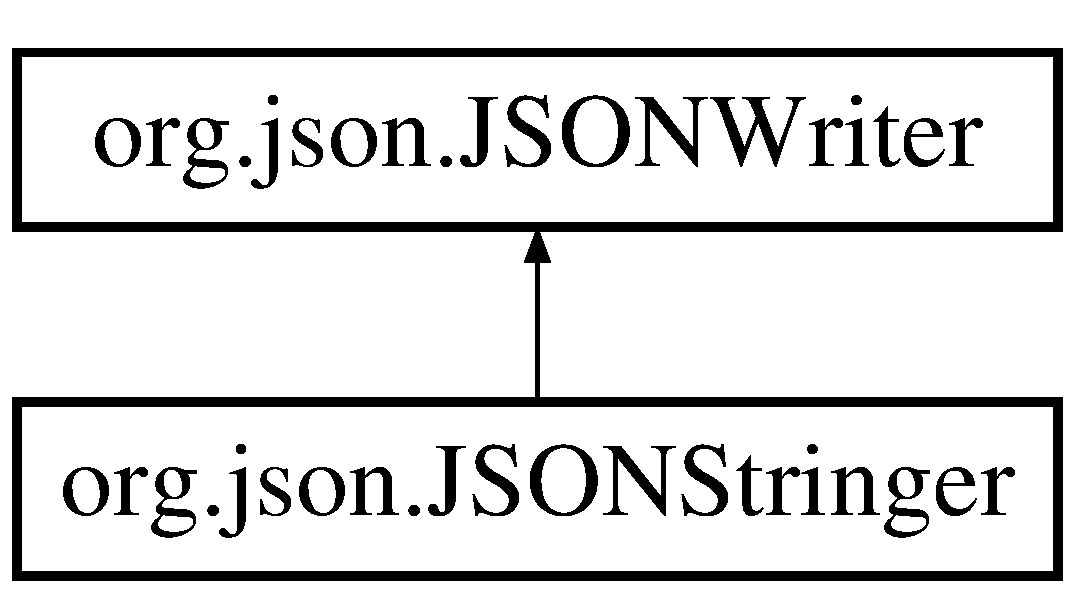
\includegraphics[height=2.000000cm]{classorg_1_1json_1_1_j_s_o_n_stringer}
\end{center}
\end{figure}
\subsection*{Public Member Functions}
\begin{DoxyCompactItemize}
\item 
\hyperlink{classorg_1_1json_1_1_j_s_o_n_stringer_a36d3accdcf3f40434edd9c33b414d3f9}{J\-S\-O\-N\-Stringer} ()
\item 
String \hyperlink{classorg_1_1json_1_1_j_s_o_n_stringer_a2e7f28e99eb46f767b5df8a669e774b4}{to\-String} ()
\end{DoxyCompactItemize}
\subsection*{Additional Inherited Members}


\subsection{Detailed Description}
\hyperlink{classorg_1_1json_1_1_j_s_o_n_stringer}{J\-S\-O\-N\-Stringer} provides a quick and convenient way of producing J\-S\-O\-N text. The texts produced strictly conform to J\-S\-O\-N syntax rules. No whitespace is added, so the results are ready for transmission or storage. Each instance of \hyperlink{classorg_1_1json_1_1_j_s_o_n_stringer}{J\-S\-O\-N\-Stringer} can produce one J\-S\-O\-N text. 

A \hyperlink{classorg_1_1json_1_1_j_s_o_n_stringer}{J\-S\-O\-N\-Stringer} instance provides a {\ttfamily value} method for appending values to the text, and a {\ttfamily key} method for adding keys before values in objects. There are {\ttfamily array} and {\ttfamily end\-Array} methods that make and bound array values, and {\ttfamily object} and {\ttfamily end\-Object} methods which make and bound object values. All of these methods return the \hyperlink{classorg_1_1json_1_1_j_s_o_n_writer}{J\-S\-O\-N\-Writer} instance, permitting cascade style. For example, 
\begin{DoxyPre}
myString = new \hyperlink{classorg_1_1json_1_1_j_s_o_n_stringer_a36d3accdcf3f40434edd9c33b414d3f9}{JSONStringer()}
    .\hyperlink{classorg_1_1json_1_1_j_s_o_n_writer_a50ed212b9c8c9f6a57c3ddfc6bf3126a}{object()}
        .key("JSON")
        .value("Hello, World!")
    .\hyperlink{classorg_1_1json_1_1_j_s_o_n_writer_a25cc931ef86998c61f08b1d5eff22146}{endObject()}
    .\hyperlink{classorg_1_1json_1_1_j_s_o_n_stringer_a2e7f28e99eb46f767b5df8a669e774b4}{toString()};\end{DoxyPre}
 which produces the string 
\begin{DoxyPre}
\{"JSON":"Hello, World!"\}\end{DoxyPre}
 

The first method called must be {\ttfamily array} or {\ttfamily object}. There are no methods for adding commas or colons. \hyperlink{classorg_1_1json_1_1_j_s_o_n_stringer}{J\-S\-O\-N\-Stringer} adds them for you. Objects and arrays can be nested up to 20 levels deep. 

This can sometimes be easier than using a \hyperlink{classorg_1_1json_1_1_j_s_o_n_object}{J\-S\-O\-N\-Object} to build a string. \begin{DoxyAuthor}{Author}
J\-S\-O\-N.\-org 
\end{DoxyAuthor}
\begin{DoxyVersion}{Version}
2008-\/09-\/18 
\end{DoxyVersion}


Definition at line 59 of file J\-S\-O\-N\-Stringer.\-java.



\subsection{Constructor \& Destructor Documentation}
\hypertarget{classorg_1_1json_1_1_j_s_o_n_stringer_a36d3accdcf3f40434edd9c33b414d3f9}{\index{org\-::json\-::\-J\-S\-O\-N\-Stringer@{org\-::json\-::\-J\-S\-O\-N\-Stringer}!J\-S\-O\-N\-Stringer@{J\-S\-O\-N\-Stringer}}
\index{J\-S\-O\-N\-Stringer@{J\-S\-O\-N\-Stringer}!org::json::JSONStringer@{org\-::json\-::\-J\-S\-O\-N\-Stringer}}
\subsubsection[{J\-S\-O\-N\-Stringer}]{\setlength{\rightskip}{0pt plus 5cm}org.\-json.\-J\-S\-O\-N\-Stringer.\-J\-S\-O\-N\-Stringer (
\begin{DoxyParamCaption}
{}
\end{DoxyParamCaption}
)}}\label{classorg_1_1json_1_1_j_s_o_n_stringer_a36d3accdcf3f40434edd9c33b414d3f9}
Make a fresh \hyperlink{classorg_1_1json_1_1_j_s_o_n_stringer}{J\-S\-O\-N\-Stringer}. It can be used to build one J\-S\-O\-N text. 

Definition at line 63 of file J\-S\-O\-N\-Stringer.\-java.


\begin{DoxyCode}
63                           \{
64         super(\textcolor{keyword}{new} StringWriter());
65     \}
\end{DoxyCode}


\subsection{Member Function Documentation}
\hypertarget{classorg_1_1json_1_1_j_s_o_n_stringer_a2e7f28e99eb46f767b5df8a669e774b4}{\index{org\-::json\-::\-J\-S\-O\-N\-Stringer@{org\-::json\-::\-J\-S\-O\-N\-Stringer}!to\-String@{to\-String}}
\index{to\-String@{to\-String}!org::json::JSONStringer@{org\-::json\-::\-J\-S\-O\-N\-Stringer}}
\subsubsection[{to\-String}]{\setlength{\rightskip}{0pt plus 5cm}String org.\-json.\-J\-S\-O\-N\-Stringer.\-to\-String (
\begin{DoxyParamCaption}
{}
\end{DoxyParamCaption}
)}}\label{classorg_1_1json_1_1_j_s_o_n_stringer_a2e7f28e99eb46f767b5df8a669e774b4}
Return the J\-S\-O\-N text. This method is used to obtain the product of the \hyperlink{classorg_1_1json_1_1_j_s_o_n_stringer}{J\-S\-O\-N\-Stringer} instance. It will return {\ttfamily null} if there was a problem in the construction of the J\-S\-O\-N text (such as the calls to {\ttfamily array} were not properly balanced with calls to {\ttfamily end\-Array}). \begin{DoxyReturn}{Returns}
The J\-S\-O\-N text. 
\end{DoxyReturn}


Definition at line 75 of file J\-S\-O\-N\-Stringer.\-java.



References org.\-json.\-J\-S\-O\-N\-Writer.\-mode, and org.\-json.\-J\-S\-O\-N\-Writer.\-writer.


\begin{DoxyCode}
75                              \{
76         \textcolor{keywordflow}{return} this.\hyperlink{classorg_1_1json_1_1_j_s_o_n_writer_acabe6b245b148eabfaa3cf975f98073f}{mode} == \textcolor{charliteral}{'d'} ? this.\hyperlink{classorg_1_1json_1_1_j_s_o_n_writer_ae5398a9b83a17ab31c993c52fc1c8e06}{writer}.toString() : null;
77     \}
\end{DoxyCode}


The documentation for this class was generated from the following file\-:\begin{DoxyCompactItemize}
\item 
org/json/\hyperlink{_j_s_o_n_stringer_8java}{J\-S\-O\-N\-Stringer.\-java}\end{DoxyCompactItemize}

\hypertarget{classorg_1_1json_1_1_j_s_o_n_tokener}{\section{org.\-json.\-J\-S\-O\-N\-Tokener Class Reference}
\label{classorg_1_1json_1_1_j_s_o_n_tokener}\index{org.\-json.\-J\-S\-O\-N\-Tokener@{org.\-json.\-J\-S\-O\-N\-Tokener}}
}
Inheritance diagram for org.\-json.\-J\-S\-O\-N\-Tokener\-:\begin{figure}[H]
\begin{center}
\leavevmode
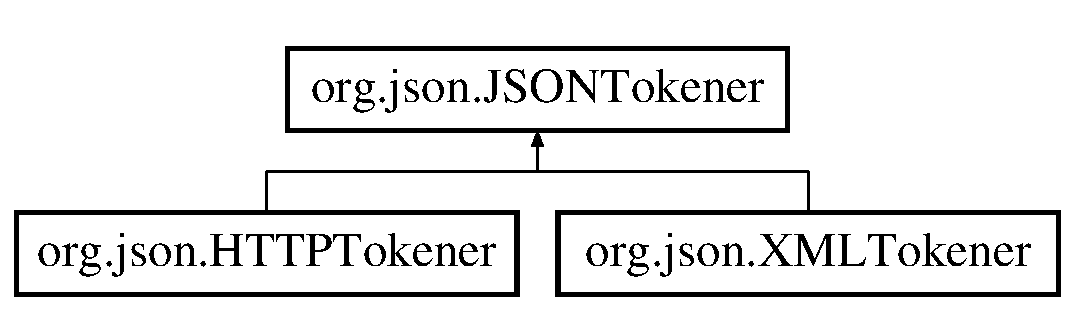
\includegraphics[height=2.000000cm]{classorg_1_1json_1_1_j_s_o_n_tokener}
\end{center}
\end{figure}
\subsection*{Public Member Functions}
\begin{DoxyCompactItemize}
\item 
\hyperlink{classorg_1_1json_1_1_j_s_o_n_tokener_ab4cd37e4683e88bced2c8e0433bb31b4}{J\-S\-O\-N\-Tokener} (Reader \hyperlink{classorg_1_1json_1_1_j_s_o_n_tokener_a41cf54327cbc4429da0e76ea032d9978}{reader})
\item 
\hyperlink{classorg_1_1json_1_1_j_s_o_n_tokener_a936053c6406cd75b0a7801d6e6de7108}{J\-S\-O\-N\-Tokener} (Input\-Stream input\-Stream)  throws J\-S\-O\-N\-Exception 
\item 
\hyperlink{classorg_1_1json_1_1_j_s_o_n_tokener_ab56cccc925fc2b4042af4b0d3de6a874}{J\-S\-O\-N\-Tokener} (String s)
\item 
void \hyperlink{classorg_1_1json_1_1_j_s_o_n_tokener_aa2eafdef7304777a457f3e66cc0e668b}{back} ()  throws J\-S\-O\-N\-Exception 
\item 
boolean \hyperlink{classorg_1_1json_1_1_j_s_o_n_tokener_a767d3f6c8313e03bc3dfb4fdc495294c}{end} ()
\item 
boolean \hyperlink{classorg_1_1json_1_1_j_s_o_n_tokener_afb0edb7fd38ed9c55470055d46aedd3a}{more} ()  throws J\-S\-O\-N\-Exception 
\item 
char \hyperlink{classorg_1_1json_1_1_j_s_o_n_tokener_ae129753dbe43ea50aa34e3c06773fdfb}{next} ()  throws J\-S\-O\-N\-Exception 
\item 
char \hyperlink{classorg_1_1json_1_1_j_s_o_n_tokener_a3525fe5f3f7767e7130fbe65de1d811e}{next} (char c)  throws J\-S\-O\-N\-Exception 
\item 
String \hyperlink{classorg_1_1json_1_1_j_s_o_n_tokener_a79e7c90c5b0ad4b83113c6df5834d2e8}{next} (int n)  throws J\-S\-O\-N\-Exception 
\item 
char \hyperlink{classorg_1_1json_1_1_j_s_o_n_tokener_ad675aa7419ea153d54a72e1fced1e08f}{next\-Clean} ()  throws J\-S\-O\-N\-Exception 
\item 
String \hyperlink{classorg_1_1json_1_1_j_s_o_n_tokener_af5622e7beb53a5290a7e18f8b8111ee5}{next\-String} (char quote)  throws J\-S\-O\-N\-Exception 
\item 
String \hyperlink{classorg_1_1json_1_1_j_s_o_n_tokener_a6d2f6ecc7488657d6a49ff27861599d4}{next\-To} (char delimiter)  throws J\-S\-O\-N\-Exception 
\item 
String \hyperlink{classorg_1_1json_1_1_j_s_o_n_tokener_a4db4f33d395593dacff7852feb51b9ae}{next\-To} (String delimiters)  throws J\-S\-O\-N\-Exception 
\item 
Object \hyperlink{classorg_1_1json_1_1_j_s_o_n_tokener_a9a139d1ce942c4693ca7268567b7def3}{next\-Value} ()  throws J\-S\-O\-N\-Exception 
\item 
char \hyperlink{classorg_1_1json_1_1_j_s_o_n_tokener_a780c7bb828073c40457b5692b06ec554}{skip\-To} (char to)  throws J\-S\-O\-N\-Exception 
\item 
\hyperlink{classorg_1_1json_1_1_j_s_o_n_exception}{J\-S\-O\-N\-Exception} \hyperlink{classorg_1_1json_1_1_j_s_o_n_tokener_a467f559950c039f28394ce3a0d2659ca}{syntax\-Error} (String message)
\item 
String \hyperlink{classorg_1_1json_1_1_j_s_o_n_tokener_a7015cb77bed5c6fdacfbfb7f2cf6effb}{to\-String} ()
\end{DoxyCompactItemize}
\subsection*{Static Public Member Functions}
\begin{DoxyCompactItemize}
\item 
static int \hyperlink{classorg_1_1json_1_1_j_s_o_n_tokener_a3ef8a20486fe58173ff9ac49e3dd7467}{dehexchar} (char c)
\end{DoxyCompactItemize}
\subsection*{Private Attributes}
\begin{DoxyCompactItemize}
\item 
long \hyperlink{classorg_1_1json_1_1_j_s_o_n_tokener_a1d8ca24139964e139f7b020d7cc4202e}{character}
\item 
boolean \hyperlink{classorg_1_1json_1_1_j_s_o_n_tokener_a17b6112399b7b89f4152e3d7178aeed8}{eof}
\item 
long \hyperlink{classorg_1_1json_1_1_j_s_o_n_tokener_aee137d262ad66a4cf877626a5549a69b}{index}
\item 
long \hyperlink{classorg_1_1json_1_1_j_s_o_n_tokener_ad906cc46c2380d59b17549770823fb60}{line}
\item 
char \hyperlink{classorg_1_1json_1_1_j_s_o_n_tokener_a3bd1cd482f2a855d74b319e7d38366c5}{previous}
\item 
Reader \hyperlink{classorg_1_1json_1_1_j_s_o_n_tokener_a41cf54327cbc4429da0e76ea032d9978}{reader}
\item 
boolean \hyperlink{classorg_1_1json_1_1_j_s_o_n_tokener_a15d3fdb7ac79686ded489fe1885bab49}{use\-Previous}
\end{DoxyCompactItemize}


\subsection{Detailed Description}
A \hyperlink{classorg_1_1json_1_1_j_s_o_n_tokener}{J\-S\-O\-N\-Tokener} takes a source string and extracts characters and tokens from it. It is used by the \hyperlink{classorg_1_1json_1_1_j_s_o_n_object}{J\-S\-O\-N\-Object} and \hyperlink{classorg_1_1json_1_1_j_s_o_n_array}{J\-S\-O\-N\-Array} constructors to parse J\-S\-O\-N source strings. \begin{DoxyAuthor}{Author}
J\-S\-O\-N.\-org 
\end{DoxyAuthor}
\begin{DoxyVersion}{Version}
2012-\/02-\/16 
\end{DoxyVersion}


Definition at line 41 of file J\-S\-O\-N\-Tokener.\-java.



\subsection{Constructor \& Destructor Documentation}
\hypertarget{classorg_1_1json_1_1_j_s_o_n_tokener_ab4cd37e4683e88bced2c8e0433bb31b4}{\index{org\-::json\-::\-J\-S\-O\-N\-Tokener@{org\-::json\-::\-J\-S\-O\-N\-Tokener}!J\-S\-O\-N\-Tokener@{J\-S\-O\-N\-Tokener}}
\index{J\-S\-O\-N\-Tokener@{J\-S\-O\-N\-Tokener}!org::json::JSONTokener@{org\-::json\-::\-J\-S\-O\-N\-Tokener}}
\subsubsection[{J\-S\-O\-N\-Tokener}]{\setlength{\rightskip}{0pt plus 5cm}org.\-json.\-J\-S\-O\-N\-Tokener.\-J\-S\-O\-N\-Tokener (
\begin{DoxyParamCaption}
\item[{Reader}]{reader}
\end{DoxyParamCaption}
)}}\label{classorg_1_1json_1_1_j_s_o_n_tokener_ab4cd37e4683e88bced2c8e0433bb31b4}
Construct a \hyperlink{classorg_1_1json_1_1_j_s_o_n_tokener}{J\-S\-O\-N\-Tokener} from a Reader.


\begin{DoxyParams}{Parameters}
{\em reader} & A reader. \\
\hline
\end{DoxyParams}


Definition at line 57 of file J\-S\-O\-N\-Tokener.\-java.



References org.\-json.\-J\-S\-O\-N\-Tokener.\-character, org.\-json.\-J\-S\-O\-N\-Tokener.\-eof, org.\-json.\-J\-S\-O\-N\-Tokener.\-index, org.\-json.\-J\-S\-O\-N\-Tokener.\-line, org.\-json.\-J\-S\-O\-N\-Tokener.\-previous, and org.\-json.\-J\-S\-O\-N\-Tokener.\-use\-Previous.


\begin{DoxyCode}
57                                       \{
58         this.\hyperlink{classorg_1_1json_1_1_j_s_o_n_tokener_a41cf54327cbc4429da0e76ea032d9978}{reader} = \hyperlink{classorg_1_1json_1_1_j_s_o_n_tokener_a41cf54327cbc4429da0e76ea032d9978}{reader}.markSupported()
59             ? \hyperlink{classorg_1_1json_1_1_j_s_o_n_tokener_a41cf54327cbc4429da0e76ea032d9978}{reader}
60             : \textcolor{keyword}{new} BufferedReader(\hyperlink{classorg_1_1json_1_1_j_s_o_n_tokener_a41cf54327cbc4429da0e76ea032d9978}{reader});
61         this.\hyperlink{classorg_1_1json_1_1_j_s_o_n_tokener_a17b6112399b7b89f4152e3d7178aeed8}{eof} = \textcolor{keyword}{false};
62         this.\hyperlink{classorg_1_1json_1_1_j_s_o_n_tokener_a15d3fdb7ac79686ded489fe1885bab49}{usePrevious} = \textcolor{keyword}{false};
63         this.\hyperlink{classorg_1_1json_1_1_j_s_o_n_tokener_a3bd1cd482f2a855d74b319e7d38366c5}{previous} = 0;
64         this.\hyperlink{classorg_1_1json_1_1_j_s_o_n_tokener_aee137d262ad66a4cf877626a5549a69b}{index} = 0;
65         this.\hyperlink{classorg_1_1json_1_1_j_s_o_n_tokener_a1d8ca24139964e139f7b020d7cc4202e}{character} = 1;
66         this.\hyperlink{classorg_1_1json_1_1_j_s_o_n_tokener_ad906cc46c2380d59b17549770823fb60}{line} = 1;
67     \}
\end{DoxyCode}
\hypertarget{classorg_1_1json_1_1_j_s_o_n_tokener_a936053c6406cd75b0a7801d6e6de7108}{\index{org\-::json\-::\-J\-S\-O\-N\-Tokener@{org\-::json\-::\-J\-S\-O\-N\-Tokener}!J\-S\-O\-N\-Tokener@{J\-S\-O\-N\-Tokener}}
\index{J\-S\-O\-N\-Tokener@{J\-S\-O\-N\-Tokener}!org::json::JSONTokener@{org\-::json\-::\-J\-S\-O\-N\-Tokener}}
\subsubsection[{J\-S\-O\-N\-Tokener}]{\setlength{\rightskip}{0pt plus 5cm}org.\-json.\-J\-S\-O\-N\-Tokener.\-J\-S\-O\-N\-Tokener (
\begin{DoxyParamCaption}
\item[{Input\-Stream}]{input\-Stream}
\end{DoxyParamCaption}
) throws {\bf J\-S\-O\-N\-Exception}}}\label{classorg_1_1json_1_1_j_s_o_n_tokener_a936053c6406cd75b0a7801d6e6de7108}
Construct a \hyperlink{classorg_1_1json_1_1_j_s_o_n_tokener}{J\-S\-O\-N\-Tokener} from an Input\-Stream. 

Definition at line 73 of file J\-S\-O\-N\-Tokener.\-java.


\begin{DoxyCode}
73                                                                      \{
74         \textcolor{keyword}{this}(\textcolor{keyword}{new} InputStreamReader(inputStream));
75     \}
\end{DoxyCode}
\hypertarget{classorg_1_1json_1_1_j_s_o_n_tokener_ab56cccc925fc2b4042af4b0d3de6a874}{\index{org\-::json\-::\-J\-S\-O\-N\-Tokener@{org\-::json\-::\-J\-S\-O\-N\-Tokener}!J\-S\-O\-N\-Tokener@{J\-S\-O\-N\-Tokener}}
\index{J\-S\-O\-N\-Tokener@{J\-S\-O\-N\-Tokener}!org::json::JSONTokener@{org\-::json\-::\-J\-S\-O\-N\-Tokener}}
\subsubsection[{J\-S\-O\-N\-Tokener}]{\setlength{\rightskip}{0pt plus 5cm}org.\-json.\-J\-S\-O\-N\-Tokener.\-J\-S\-O\-N\-Tokener (
\begin{DoxyParamCaption}
\item[{String}]{s}
\end{DoxyParamCaption}
)}}\label{classorg_1_1json_1_1_j_s_o_n_tokener_ab56cccc925fc2b4042af4b0d3de6a874}
Construct a \hyperlink{classorg_1_1json_1_1_j_s_o_n_tokener}{J\-S\-O\-N\-Tokener} from a string.


\begin{DoxyParams}{Parameters}
{\em s} & A source string. \\
\hline
\end{DoxyParams}


Definition at line 83 of file J\-S\-O\-N\-Tokener.\-java.


\begin{DoxyCode}
83                                  \{
84         \textcolor{keyword}{this}(\textcolor{keyword}{new} StringReader(s));
85     \}
\end{DoxyCode}


\subsection{Member Function Documentation}
\hypertarget{classorg_1_1json_1_1_j_s_o_n_tokener_aa2eafdef7304777a457f3e66cc0e668b}{\index{org\-::json\-::\-J\-S\-O\-N\-Tokener@{org\-::json\-::\-J\-S\-O\-N\-Tokener}!back@{back}}
\index{back@{back}!org::json::JSONTokener@{org\-::json\-::\-J\-S\-O\-N\-Tokener}}
\subsubsection[{back}]{\setlength{\rightskip}{0pt plus 5cm}void org.\-json.\-J\-S\-O\-N\-Tokener.\-back (
\begin{DoxyParamCaption}
{}
\end{DoxyParamCaption}
) throws {\bf J\-S\-O\-N\-Exception}}}\label{classorg_1_1json_1_1_j_s_o_n_tokener_aa2eafdef7304777a457f3e66cc0e668b}
Back up one character. This provides a sort of lookahead capability, so that you can test for a digit or letter before attempting to parse the next number or identifier. 

Definition at line 93 of file J\-S\-O\-N\-Tokener.\-java.



References org.\-json.\-J\-S\-O\-N\-Tokener.\-character, org.\-json.\-J\-S\-O\-N\-Tokener.\-eof, org.\-json.\-J\-S\-O\-N\-Tokener.\-index, and org.\-json.\-J\-S\-O\-N\-Tokener.\-use\-Previous.



Referenced by org.\-json.\-J\-S\-O\-N\-Tokener.\-more(), org.\-json.\-X\-M\-L\-Tokener.\-next\-Content(), org.\-json.\-X\-M\-L\-Tokener.\-next\-Meta(), org.\-json.\-J\-S\-O\-N\-Tokener.\-next\-To(), org.\-json.\-X\-M\-L\-Tokener.\-next\-Token(), org.\-json.\-J\-S\-O\-N\-Tokener.\-next\-Value(), and org.\-json.\-J\-S\-O\-N\-Tokener.\-skip\-To().


\begin{DoxyCode}
93                                             \{
94         \textcolor{keywordflow}{if} (this.\hyperlink{classorg_1_1json_1_1_j_s_o_n_tokener_a15d3fdb7ac79686ded489fe1885bab49}{usePrevious} || this.\hyperlink{classorg_1_1json_1_1_j_s_o_n_tokener_aee137d262ad66a4cf877626a5549a69b}{index} <= 0) \{
95             \textcolor{keywordflow}{throw} \textcolor{keyword}{new} JSONException(\textcolor{stringliteral}{"Stepping back two steps is not supported"});
96         \}
97         this.\hyperlink{classorg_1_1json_1_1_j_s_o_n_tokener_aee137d262ad66a4cf877626a5549a69b}{index} -= 1;
98         this.\hyperlink{classorg_1_1json_1_1_j_s_o_n_tokener_a1d8ca24139964e139f7b020d7cc4202e}{character} -= 1;
99         this.\hyperlink{classorg_1_1json_1_1_j_s_o_n_tokener_a15d3fdb7ac79686ded489fe1885bab49}{usePrevious} = \textcolor{keyword}{true};
100         this.\hyperlink{classorg_1_1json_1_1_j_s_o_n_tokener_a17b6112399b7b89f4152e3d7178aeed8}{eof} = \textcolor{keyword}{false};
101     \}
\end{DoxyCode}
\hypertarget{classorg_1_1json_1_1_j_s_o_n_tokener_a3ef8a20486fe58173ff9ac49e3dd7467}{\index{org\-::json\-::\-J\-S\-O\-N\-Tokener@{org\-::json\-::\-J\-S\-O\-N\-Tokener}!dehexchar@{dehexchar}}
\index{dehexchar@{dehexchar}!org::json::JSONTokener@{org\-::json\-::\-J\-S\-O\-N\-Tokener}}
\subsubsection[{dehexchar}]{\setlength{\rightskip}{0pt plus 5cm}static int org.\-json.\-J\-S\-O\-N\-Tokener.\-dehexchar (
\begin{DoxyParamCaption}
\item[{char}]{c}
\end{DoxyParamCaption}
)\hspace{0.3cm}{\ttfamily [static]}}}\label{classorg_1_1json_1_1_j_s_o_n_tokener_a3ef8a20486fe58173ff9ac49e3dd7467}
Get the hex value of a character (base16). 
\begin{DoxyParams}{Parameters}
{\em c} & A character between '0' and '9' or between 'A' and 'F' or between 'a' and 'f'. \\
\hline
\end{DoxyParams}
\begin{DoxyReturn}{Returns}
An int between 0 and 15, or -\/1 if c was not a hex digit. 
\end{DoxyReturn}


Definition at line 110 of file J\-S\-O\-N\-Tokener.\-java.



Referenced by org.\-json.\-Cookie.\-unescape().


\begin{DoxyCode}
110                                         \{
111         \textcolor{keywordflow}{if} (c >= \textcolor{charliteral}{'0'} && c <= \textcolor{charliteral}{'9'}) \{
112             \textcolor{keywordflow}{return} c - \textcolor{charliteral}{'0'};
113         \}
114         \textcolor{keywordflow}{if} (c >= \textcolor{charliteral}{'A'} && c <= \textcolor{charliteral}{'F'}) \{
115             \textcolor{keywordflow}{return} c - (\textcolor{charliteral}{'A'} - 10);
116         \}
117         \textcolor{keywordflow}{if} (c >= \textcolor{charliteral}{'a'} && c <= \textcolor{charliteral}{'f'}) \{
118             \textcolor{keywordflow}{return} c - (\textcolor{charliteral}{'a'} - 10);
119         \}
120         \textcolor{keywordflow}{return} -1;
121     \}
\end{DoxyCode}
\hypertarget{classorg_1_1json_1_1_j_s_o_n_tokener_a767d3f6c8313e03bc3dfb4fdc495294c}{\index{org\-::json\-::\-J\-S\-O\-N\-Tokener@{org\-::json\-::\-J\-S\-O\-N\-Tokener}!end@{end}}
\index{end@{end}!org::json::JSONTokener@{org\-::json\-::\-J\-S\-O\-N\-Tokener}}
\subsubsection[{end}]{\setlength{\rightskip}{0pt plus 5cm}boolean org.\-json.\-J\-S\-O\-N\-Tokener.\-end (
\begin{DoxyParamCaption}
{}
\end{DoxyParamCaption}
)}}\label{classorg_1_1json_1_1_j_s_o_n_tokener_a767d3f6c8313e03bc3dfb4fdc495294c}


Definition at line 123 of file J\-S\-O\-N\-Tokener.\-java.



References org.\-json.\-J\-S\-O\-N\-Tokener.\-eof, and org.\-json.\-J\-S\-O\-N\-Tokener.\-use\-Previous.



Referenced by org.\-json.\-J\-S\-O\-N\-Tokener.\-more(), org.\-json.\-J\-S\-O\-N\-Tokener.\-next(), and org.\-json.\-X\-M\-L\-Tokener.\-next\-C\-D\-A\-T\-A().


\begin{DoxyCode}
123                          \{
124         \textcolor{keywordflow}{return} this.\hyperlink{classorg_1_1json_1_1_j_s_o_n_tokener_a17b6112399b7b89f4152e3d7178aeed8}{eof} && !this.\hyperlink{classorg_1_1json_1_1_j_s_o_n_tokener_a15d3fdb7ac79686ded489fe1885bab49}{usePrevious};
125     \}
\end{DoxyCode}
\hypertarget{classorg_1_1json_1_1_j_s_o_n_tokener_afb0edb7fd38ed9c55470055d46aedd3a}{\index{org\-::json\-::\-J\-S\-O\-N\-Tokener@{org\-::json\-::\-J\-S\-O\-N\-Tokener}!more@{more}}
\index{more@{more}!org::json::JSONTokener@{org\-::json\-::\-J\-S\-O\-N\-Tokener}}
\subsubsection[{more}]{\setlength{\rightskip}{0pt plus 5cm}boolean org.\-json.\-J\-S\-O\-N\-Tokener.\-more (
\begin{DoxyParamCaption}
{}
\end{DoxyParamCaption}
) throws {\bf J\-S\-O\-N\-Exception}}}\label{classorg_1_1json_1_1_j_s_o_n_tokener_afb0edb7fd38ed9c55470055d46aedd3a}
Determine if the source string still contains characters that \hyperlink{classorg_1_1json_1_1_j_s_o_n_tokener_ae129753dbe43ea50aa34e3c06773fdfb}{next()} can consume. \begin{DoxyReturn}{Returns}
true if not yet at the end of the source. 
\end{DoxyReturn}


Definition at line 133 of file J\-S\-O\-N\-Tokener.\-java.



References org.\-json.\-J\-S\-O\-N\-Tokener.\-back(), org.\-json.\-J\-S\-O\-N\-Tokener.\-end(), and org.\-json.\-J\-S\-O\-N\-Tokener.\-next().



Referenced by org.\-json.\-Cookie\-List.\-to\-J\-S\-O\-N\-Object(), org.\-json.\-H\-T\-T\-P.\-to\-J\-S\-O\-N\-Object(), org.\-json.\-Cookie.\-to\-J\-S\-O\-N\-Object(), and org.\-json.\-X\-M\-L.\-to\-J\-S\-O\-N\-Object().


\begin{DoxyCode}
133                                                \{
134         this.\hyperlink{classorg_1_1json_1_1_j_s_o_n_tokener_ae129753dbe43ea50aa34e3c06773fdfb}{next}();
135         \textcolor{keywordflow}{if} (this.\hyperlink{classorg_1_1json_1_1_j_s_o_n_tokener_a767d3f6c8313e03bc3dfb4fdc495294c}{end}()) \{
136             \textcolor{keywordflow}{return} \textcolor{keyword}{false};
137         \}
138         this.\hyperlink{classorg_1_1json_1_1_j_s_o_n_tokener_aa2eafdef7304777a457f3e66cc0e668b}{back}();
139         \textcolor{keywordflow}{return} \textcolor{keyword}{true};
140     \}
\end{DoxyCode}
\hypertarget{classorg_1_1json_1_1_j_s_o_n_tokener_ae129753dbe43ea50aa34e3c06773fdfb}{\index{org\-::json\-::\-J\-S\-O\-N\-Tokener@{org\-::json\-::\-J\-S\-O\-N\-Tokener}!next@{next}}
\index{next@{next}!org::json::JSONTokener@{org\-::json\-::\-J\-S\-O\-N\-Tokener}}
\subsubsection[{next}]{\setlength{\rightskip}{0pt plus 5cm}char org.\-json.\-J\-S\-O\-N\-Tokener.\-next (
\begin{DoxyParamCaption}
{}
\end{DoxyParamCaption}
) throws {\bf J\-S\-O\-N\-Exception}}}\label{classorg_1_1json_1_1_j_s_o_n_tokener_ae129753dbe43ea50aa34e3c06773fdfb}
Get the next character in the source string.

\begin{DoxyReturn}{Returns}
The next character, or 0 if past the end of the source string. 
\end{DoxyReturn}


Definition at line 148 of file J\-S\-O\-N\-Tokener.\-java.



References org.\-json.\-J\-S\-O\-N\-Tokener.\-character, org.\-json.\-J\-S\-O\-N\-Tokener.\-eof, org.\-json.\-J\-S\-O\-N\-Tokener.\-index, org.\-json.\-J\-S\-O\-N\-Tokener.\-line, org.\-json.\-J\-S\-O\-N\-Tokener.\-previous, org.\-json.\-J\-S\-O\-N\-Tokener.\-reader, and org.\-json.\-J\-S\-O\-N\-Tokener.\-use\-Previous.



Referenced by org.\-json.\-J\-S\-O\-N\-Tokener.\-more(), org.\-json.\-J\-S\-O\-N\-Tokener.\-next(), org.\-json.\-X\-M\-L\-Tokener.\-next\-C\-D\-A\-T\-A(), org.\-json.\-J\-S\-O\-N\-Tokener.\-next\-Clean(), org.\-json.\-X\-M\-L\-Tokener.\-next\-Content(), org.\-json.\-X\-M\-L\-Tokener.\-next\-Entity(), org.\-json.\-X\-M\-L\-Tokener.\-next\-Meta(), org.\-json.\-J\-S\-O\-N\-Tokener.\-next\-String(), org.\-json.\-J\-S\-O\-N\-Tokener.\-next\-To(), org.\-json.\-H\-T\-T\-P\-Tokener.\-next\-Token(), org.\-json.\-X\-M\-L\-Tokener.\-next\-Token(), org.\-json.\-J\-S\-O\-N\-Tokener.\-next\-Value(), org.\-json.\-X\-M\-L\-Tokener.\-skip\-Past(), org.\-json.\-J\-S\-O\-N\-Tokener.\-skip\-To(), org.\-json.\-Cookie\-List.\-to\-J\-S\-O\-N\-Object(), org.\-json.\-H\-T\-T\-P.\-to\-J\-S\-O\-N\-Object(), and org.\-json.\-Cookie.\-to\-J\-S\-O\-N\-Object().


\begin{DoxyCode}
148                                             \{
149         \textcolor{keywordtype}{int} c;
150         \textcolor{keywordflow}{if} (this.\hyperlink{classorg_1_1json_1_1_j_s_o_n_tokener_a15d3fdb7ac79686ded489fe1885bab49}{usePrevious}) \{
151             this.\hyperlink{classorg_1_1json_1_1_j_s_o_n_tokener_a15d3fdb7ac79686ded489fe1885bab49}{usePrevious} = \textcolor{keyword}{false};
152             c = this.\hyperlink{classorg_1_1json_1_1_j_s_o_n_tokener_a3bd1cd482f2a855d74b319e7d38366c5}{previous};
153         \} \textcolor{keywordflow}{else} \{
154             \textcolor{keywordflow}{try} \{
155                 c = this.\hyperlink{classorg_1_1json_1_1_j_s_o_n_tokener_a41cf54327cbc4429da0e76ea032d9978}{reader}.read();
156             \} \textcolor{keywordflow}{catch} (IOException exception) \{
157                 \textcolor{keywordflow}{throw} \textcolor{keyword}{new} JSONException(exception);
158             \}
159 
160             \textcolor{keywordflow}{if} (c <= 0) \{ \textcolor{comment}{// End of stream}
161                 this.\hyperlink{classorg_1_1json_1_1_j_s_o_n_tokener_a17b6112399b7b89f4152e3d7178aeed8}{eof} = \textcolor{keyword}{true};
162                 c = 0;
163             \}
164         \}
165         this.\hyperlink{classorg_1_1json_1_1_j_s_o_n_tokener_aee137d262ad66a4cf877626a5549a69b}{index} += 1;
166         \textcolor{keywordflow}{if} (this.\hyperlink{classorg_1_1json_1_1_j_s_o_n_tokener_a3bd1cd482f2a855d74b319e7d38366c5}{previous} == \textcolor{charliteral}{'\(\backslash\)r'}) \{
167             this.\hyperlink{classorg_1_1json_1_1_j_s_o_n_tokener_ad906cc46c2380d59b17549770823fb60}{line} += 1;
168             this.\hyperlink{classorg_1_1json_1_1_j_s_o_n_tokener_a1d8ca24139964e139f7b020d7cc4202e}{character} = c == \textcolor{charliteral}{'\(\backslash\)n'} ? 0 : 1;
169         \} \textcolor{keywordflow}{else} \textcolor{keywordflow}{if} (c == \textcolor{charliteral}{'\(\backslash\)n'}) \{
170             this.\hyperlink{classorg_1_1json_1_1_j_s_o_n_tokener_ad906cc46c2380d59b17549770823fb60}{line} += 1;
171             this.\hyperlink{classorg_1_1json_1_1_j_s_o_n_tokener_a1d8ca24139964e139f7b020d7cc4202e}{character} = 0;
172         \} \textcolor{keywordflow}{else} \{
173             this.\hyperlink{classorg_1_1json_1_1_j_s_o_n_tokener_a1d8ca24139964e139f7b020d7cc4202e}{character} += 1;
174         \}
175         this.\hyperlink{classorg_1_1json_1_1_j_s_o_n_tokener_a3bd1cd482f2a855d74b319e7d38366c5}{previous} = (char) c;
176         \textcolor{keywordflow}{return} this.\hyperlink{classorg_1_1json_1_1_j_s_o_n_tokener_a3bd1cd482f2a855d74b319e7d38366c5}{previous};
177     \}
\end{DoxyCode}
\hypertarget{classorg_1_1json_1_1_j_s_o_n_tokener_a3525fe5f3f7767e7130fbe65de1d811e}{\index{org\-::json\-::\-J\-S\-O\-N\-Tokener@{org\-::json\-::\-J\-S\-O\-N\-Tokener}!next@{next}}
\index{next@{next}!org::json::JSONTokener@{org\-::json\-::\-J\-S\-O\-N\-Tokener}}
\subsubsection[{next}]{\setlength{\rightskip}{0pt plus 5cm}char org.\-json.\-J\-S\-O\-N\-Tokener.\-next (
\begin{DoxyParamCaption}
\item[{char}]{c}
\end{DoxyParamCaption}
) throws {\bf J\-S\-O\-N\-Exception}}}\label{classorg_1_1json_1_1_j_s_o_n_tokener_a3525fe5f3f7767e7130fbe65de1d811e}
Consume the next character, and check that it matches a specified character. 
\begin{DoxyParams}{Parameters}
{\em c} & The character to match. \\
\hline
\end{DoxyParams}
\begin{DoxyReturn}{Returns}
The character. 
\end{DoxyReturn}

\begin{DoxyExceptions}{Exceptions}
{\em \hyperlink{classorg_1_1json_1_1_j_s_o_n_exception}{J\-S\-O\-N\-Exception}} & if the character does not match. \\
\hline
\end{DoxyExceptions}


Definition at line 187 of file J\-S\-O\-N\-Tokener.\-java.



References org.\-json.\-J\-S\-O\-N\-Tokener.\-next(), and org.\-json.\-J\-S\-O\-N\-Tokener.\-syntax\-Error().


\begin{DoxyCode}
187                                                   \{
188         \textcolor{keywordtype}{char} n = this.\hyperlink{classorg_1_1json_1_1_j_s_o_n_tokener_ae129753dbe43ea50aa34e3c06773fdfb}{next}();
189         \textcolor{keywordflow}{if} (n != c) \{
190             \textcolor{keywordflow}{throw} this.\hyperlink{classorg_1_1json_1_1_j_s_o_n_tokener_a467f559950c039f28394ce3a0d2659ca}{syntaxError}(\textcolor{stringliteral}{"Expected '"} + c + \textcolor{stringliteral}{"' and instead saw '"} +
191                     n + \textcolor{stringliteral}{"'"});
192         \}
193         \textcolor{keywordflow}{return} n;
194     \}
\end{DoxyCode}
\hypertarget{classorg_1_1json_1_1_j_s_o_n_tokener_a79e7c90c5b0ad4b83113c6df5834d2e8}{\index{org\-::json\-::\-J\-S\-O\-N\-Tokener@{org\-::json\-::\-J\-S\-O\-N\-Tokener}!next@{next}}
\index{next@{next}!org::json::JSONTokener@{org\-::json\-::\-J\-S\-O\-N\-Tokener}}
\subsubsection[{next}]{\setlength{\rightskip}{0pt plus 5cm}String org.\-json.\-J\-S\-O\-N\-Tokener.\-next (
\begin{DoxyParamCaption}
\item[{int}]{n}
\end{DoxyParamCaption}
) throws {\bf J\-S\-O\-N\-Exception}}}\label{classorg_1_1json_1_1_j_s_o_n_tokener_a79e7c90c5b0ad4b83113c6df5834d2e8}
Get the next n characters.


\begin{DoxyParams}{Parameters}
{\em n} & The number of characters to take. \\
\hline
\end{DoxyParams}
\begin{DoxyReturn}{Returns}
A string of n characters. 
\end{DoxyReturn}

\begin{DoxyExceptions}{Exceptions}
{\em \hyperlink{classorg_1_1json_1_1_j_s_o_n_exception}{J\-S\-O\-N\-Exception}} & Substring bounds error if there are not n characters remaining in the source string. \\
\hline
\end{DoxyExceptions}


Definition at line 206 of file J\-S\-O\-N\-Tokener.\-java.



References org.\-json.\-J\-S\-O\-N\-Tokener.\-end(), org.\-json.\-J\-S\-O\-N\-Tokener.\-next(), and org.\-json.\-J\-S\-O\-N\-Tokener.\-syntax\-Error().


\begin{DoxyCode}
206                                                     \{
207          \textcolor{keywordflow}{if} (n == 0) \{
208              \textcolor{keywordflow}{return} \textcolor{stringliteral}{""};
209          \}
210 
211          \textcolor{keywordtype}{char}[] chars = \textcolor{keyword}{new} \textcolor{keywordtype}{char}[n];
212          \textcolor{keywordtype}{int} pos = 0;
213 
214          \textcolor{keywordflow}{while} (pos < n) \{
215              chars[pos] = this.\hyperlink{classorg_1_1json_1_1_j_s_o_n_tokener_ae129753dbe43ea50aa34e3c06773fdfb}{next}();
216              \textcolor{keywordflow}{if} (this.\hyperlink{classorg_1_1json_1_1_j_s_o_n_tokener_a767d3f6c8313e03bc3dfb4fdc495294c}{end}()) \{
217                  \textcolor{keywordflow}{throw} this.\hyperlink{classorg_1_1json_1_1_j_s_o_n_tokener_a467f559950c039f28394ce3a0d2659ca}{syntaxError}(\textcolor{stringliteral}{"Substring bounds error"});
218              \}
219              pos += 1;
220          \}
221          \textcolor{keywordflow}{return} \textcolor{keyword}{new} String(chars);
222      \}
\end{DoxyCode}
\hypertarget{classorg_1_1json_1_1_j_s_o_n_tokener_ad675aa7419ea153d54a72e1fced1e08f}{\index{org\-::json\-::\-J\-S\-O\-N\-Tokener@{org\-::json\-::\-J\-S\-O\-N\-Tokener}!next\-Clean@{next\-Clean}}
\index{next\-Clean@{next\-Clean}!org::json::JSONTokener@{org\-::json\-::\-J\-S\-O\-N\-Tokener}}
\subsubsection[{next\-Clean}]{\setlength{\rightskip}{0pt plus 5cm}char org.\-json.\-J\-S\-O\-N\-Tokener.\-next\-Clean (
\begin{DoxyParamCaption}
{}
\end{DoxyParamCaption}
) throws {\bf J\-S\-O\-N\-Exception}}}\label{classorg_1_1json_1_1_j_s_o_n_tokener_ad675aa7419ea153d54a72e1fced1e08f}
Get the next char in the string, skipping whitespace. 
\begin{DoxyExceptions}{Exceptions}
{\em \hyperlink{classorg_1_1json_1_1_j_s_o_n_exception}{J\-S\-O\-N\-Exception}} & \\
\hline
\end{DoxyExceptions}
\begin{DoxyReturn}{Returns}
A character, or 0 if there are no more characters. 
\end{DoxyReturn}


Definition at line 230 of file J\-S\-O\-N\-Tokener.\-java.



References org.\-json.\-J\-S\-O\-N\-Tokener.\-next().



Referenced by org.\-json.\-J\-S\-O\-N\-Tokener.\-next\-Value().


\begin{DoxyCode}
230                                                  \{
231         \textcolor{keywordflow}{for} (;;) \{
232             \textcolor{keywordtype}{char} c = this.\hyperlink{classorg_1_1json_1_1_j_s_o_n_tokener_ae129753dbe43ea50aa34e3c06773fdfb}{next}();
233             \textcolor{keywordflow}{if} (c == 0 || c > \textcolor{charliteral}{' '}) \{
234                 \textcolor{keywordflow}{return} c;
235             \}
236         \}
237     \}
\end{DoxyCode}
\hypertarget{classorg_1_1json_1_1_j_s_o_n_tokener_af5622e7beb53a5290a7e18f8b8111ee5}{\index{org\-::json\-::\-J\-S\-O\-N\-Tokener@{org\-::json\-::\-J\-S\-O\-N\-Tokener}!next\-String@{next\-String}}
\index{next\-String@{next\-String}!org::json::JSONTokener@{org\-::json\-::\-J\-S\-O\-N\-Tokener}}
\subsubsection[{next\-String}]{\setlength{\rightskip}{0pt plus 5cm}String org.\-json.\-J\-S\-O\-N\-Tokener.\-next\-String (
\begin{DoxyParamCaption}
\item[{char}]{quote}
\end{DoxyParamCaption}
) throws {\bf J\-S\-O\-N\-Exception}}}\label{classorg_1_1json_1_1_j_s_o_n_tokener_af5622e7beb53a5290a7e18f8b8111ee5}
Return the characters up to the next close quote character. Backslash processing is done. The formal J\-S\-O\-N format does not allow strings in single quotes, but an implementation is allowed to accept them. 
\begin{DoxyParams}{Parameters}
{\em quote} & The quoting character, either {\ttfamily "}~
\footnotesize (double quote)
\normalsize  or {\ttfamily '}~
\footnotesize (single quote)
\normalsize . \\
\hline
\end{DoxyParams}
\begin{DoxyReturn}{Returns}
A String. 
\end{DoxyReturn}

\begin{DoxyExceptions}{Exceptions}
{\em \hyperlink{classorg_1_1json_1_1_j_s_o_n_exception}{J\-S\-O\-N\-Exception}} & Unterminated string. \\
\hline
\end{DoxyExceptions}


Definition at line 251 of file J\-S\-O\-N\-Tokener.\-java.



References org.\-json.\-J\-S\-O\-N\-Tokener.\-next(), and org.\-json.\-J\-S\-O\-N\-Tokener.\-syntax\-Error().



Referenced by org.\-json.\-J\-S\-O\-N\-Tokener.\-next\-Value().


\begin{DoxyCode}
251                                                               \{
252         \textcolor{keywordtype}{char} c;
253         StringBuffer sb = \textcolor{keyword}{new} StringBuffer();
254         \textcolor{keywordflow}{for} (;;) \{
255             c = this.\hyperlink{classorg_1_1json_1_1_j_s_o_n_tokener_ae129753dbe43ea50aa34e3c06773fdfb}{next}();
256             \textcolor{keywordflow}{switch} (c) \{
257             \textcolor{keywordflow}{case} 0:
258             \textcolor{keywordflow}{case} \textcolor{charliteral}{'\(\backslash\)n'}:
259             \textcolor{keywordflow}{case} \textcolor{charliteral}{'\(\backslash\)r'}:
260                 \textcolor{keywordflow}{throw} this.\hyperlink{classorg_1_1json_1_1_j_s_o_n_tokener_a467f559950c039f28394ce3a0d2659ca}{syntaxError}(\textcolor{stringliteral}{"Unterminated string"});
261             \textcolor{keywordflow}{case} \textcolor{charliteral}{'\(\backslash\)\(\backslash\)'}:
262                 c = this.\hyperlink{classorg_1_1json_1_1_j_s_o_n_tokener_ae129753dbe43ea50aa34e3c06773fdfb}{next}();
263                 \textcolor{keywordflow}{switch} (c) \{
264                 \textcolor{keywordflow}{case} \textcolor{charliteral}{'b'}:
265                     sb.append(\textcolor{charliteral}{'\(\backslash\)b'});
266                     \textcolor{keywordflow}{break};
267                 \textcolor{keywordflow}{case} \textcolor{charliteral}{'t'}:
268                     sb.append(\textcolor{charliteral}{'\(\backslash\)t'});
269                     \textcolor{keywordflow}{break};
270                 \textcolor{keywordflow}{case} \textcolor{charliteral}{'n'}:
271                     sb.append(\textcolor{charliteral}{'\(\backslash\)n'});
272                     \textcolor{keywordflow}{break};
273                 \textcolor{keywordflow}{case} \textcolor{charliteral}{'f'}:
274                     sb.append(\textcolor{charliteral}{'\(\backslash\)f'});
275                     \textcolor{keywordflow}{break};
276                 \textcolor{keywordflow}{case} \textcolor{charliteral}{'r'}:
277                     sb.append(\textcolor{charliteral}{'\(\backslash\)r'});
278                     \textcolor{keywordflow}{break};
279                 \textcolor{keywordflow}{case} \textcolor{charliteral}{'u'}:
280                     sb.append((\textcolor{keywordtype}{char})Integer.parseInt(\textcolor{keyword}{this}.next(4), 16));
281                     \textcolor{keywordflow}{break};
282                 \textcolor{keywordflow}{case} \textcolor{charliteral}{'"'}:
283                 \textcolor{keywordflow}{case} \textcolor{charliteral}{'\(\backslash\)''}:
284                 \textcolor{keywordflow}{case} \textcolor{charliteral}{'\(\backslash\)\(\backslash\)'}:
285                 \textcolor{keywordflow}{case} \textcolor{charliteral}{'/'}:
286                     sb.append(c);
287                     \textcolor{keywordflow}{break};
288                 \textcolor{keywordflow}{default}:
289                     \textcolor{keywordflow}{throw} this.\hyperlink{classorg_1_1json_1_1_j_s_o_n_tokener_a467f559950c039f28394ce3a0d2659ca}{syntaxError}(\textcolor{stringliteral}{"Illegal escape."});
290                 \}
291                 \textcolor{keywordflow}{break};
292             \textcolor{keywordflow}{default}:
293                 \textcolor{keywordflow}{if} (c == quote) \{
294                     \textcolor{keywordflow}{return} sb.toString();
295                 \}
296                 sb.append(c);
297             \}
298         \}
299     \}
\end{DoxyCode}
\hypertarget{classorg_1_1json_1_1_j_s_o_n_tokener_a6d2f6ecc7488657d6a49ff27861599d4}{\index{org\-::json\-::\-J\-S\-O\-N\-Tokener@{org\-::json\-::\-J\-S\-O\-N\-Tokener}!next\-To@{next\-To}}
\index{next\-To@{next\-To}!org::json::JSONTokener@{org\-::json\-::\-J\-S\-O\-N\-Tokener}}
\subsubsection[{next\-To}]{\setlength{\rightskip}{0pt plus 5cm}String org.\-json.\-J\-S\-O\-N\-Tokener.\-next\-To (
\begin{DoxyParamCaption}
\item[{char}]{delimiter}
\end{DoxyParamCaption}
) throws {\bf J\-S\-O\-N\-Exception}}}\label{classorg_1_1json_1_1_j_s_o_n_tokener_a6d2f6ecc7488657d6a49ff27861599d4}
Get the text up but not including the specified character or the end of line, whichever comes first. 
\begin{DoxyParams}{Parameters}
{\em delimiter} & A delimiter character. \\
\hline
\end{DoxyParams}
\begin{DoxyReturn}{Returns}
A string. 
\end{DoxyReturn}


Definition at line 308 of file J\-S\-O\-N\-Tokener.\-java.



References org.\-json.\-J\-S\-O\-N\-Tokener.\-back(), and org.\-json.\-J\-S\-O\-N\-Tokener.\-next().



Referenced by org.\-json.\-Cookie\-List.\-to\-J\-S\-O\-N\-Object(), org.\-json.\-H\-T\-T\-P.\-to\-J\-S\-O\-N\-Object(), and org.\-json.\-Cookie.\-to\-J\-S\-O\-N\-Object().


\begin{DoxyCode}
308                                                               \{
309         StringBuffer sb = \textcolor{keyword}{new} StringBuffer();
310         \textcolor{keywordflow}{for} (;;) \{
311             \textcolor{keywordtype}{char} c = this.\hyperlink{classorg_1_1json_1_1_j_s_o_n_tokener_ae129753dbe43ea50aa34e3c06773fdfb}{next}();
312             \textcolor{keywordflow}{if} (c == delimiter || c == 0 || c == \textcolor{charliteral}{'\(\backslash\)n'} || c == \textcolor{charliteral}{'\(\backslash\)r'}) \{
313                 \textcolor{keywordflow}{if} (c != 0) \{
314                     this.\hyperlink{classorg_1_1json_1_1_j_s_o_n_tokener_aa2eafdef7304777a457f3e66cc0e668b}{back}();
315                 \}
316                 \textcolor{keywordflow}{return} sb.toString().trim();
317             \}
318             sb.append(c);
319         \}
320     \}
\end{DoxyCode}
\hypertarget{classorg_1_1json_1_1_j_s_o_n_tokener_a4db4f33d395593dacff7852feb51b9ae}{\index{org\-::json\-::\-J\-S\-O\-N\-Tokener@{org\-::json\-::\-J\-S\-O\-N\-Tokener}!next\-To@{next\-To}}
\index{next\-To@{next\-To}!org::json::JSONTokener@{org\-::json\-::\-J\-S\-O\-N\-Tokener}}
\subsubsection[{next\-To}]{\setlength{\rightskip}{0pt plus 5cm}String org.\-json.\-J\-S\-O\-N\-Tokener.\-next\-To (
\begin{DoxyParamCaption}
\item[{String}]{delimiters}
\end{DoxyParamCaption}
) throws {\bf J\-S\-O\-N\-Exception}}}\label{classorg_1_1json_1_1_j_s_o_n_tokener_a4db4f33d395593dacff7852feb51b9ae}
Get the text up but not including one of the specified delimiter characters or the end of line, whichever comes first. 
\begin{DoxyParams}{Parameters}
{\em delimiters} & A set of delimiter characters. \\
\hline
\end{DoxyParams}
\begin{DoxyReturn}{Returns}
A string, trimmed. 
\end{DoxyReturn}


Definition at line 329 of file J\-S\-O\-N\-Tokener.\-java.



References org.\-json.\-J\-S\-O\-N\-Tokener.\-back(), and org.\-json.\-J\-S\-O\-N\-Tokener.\-next().


\begin{DoxyCode}
329                                                                  \{
330         \textcolor{keywordtype}{char} c;
331         StringBuffer sb = \textcolor{keyword}{new} StringBuffer();
332         \textcolor{keywordflow}{for} (;;) \{
333             c = this.\hyperlink{classorg_1_1json_1_1_j_s_o_n_tokener_ae129753dbe43ea50aa34e3c06773fdfb}{next}();
334             \textcolor{keywordflow}{if} (delimiters.indexOf(c) >= 0 || c == 0 ||
335                     c == \textcolor{charliteral}{'\(\backslash\)n'} || c == \textcolor{charliteral}{'\(\backslash\)r'}) \{
336                 \textcolor{keywordflow}{if} (c != 0) \{
337                     this.\hyperlink{classorg_1_1json_1_1_j_s_o_n_tokener_aa2eafdef7304777a457f3e66cc0e668b}{back}();
338                 \}
339                 \textcolor{keywordflow}{return} sb.toString().trim();
340             \}
341             sb.append(c);
342         \}
343     \}
\end{DoxyCode}
\hypertarget{classorg_1_1json_1_1_j_s_o_n_tokener_a9a139d1ce942c4693ca7268567b7def3}{\index{org\-::json\-::\-J\-S\-O\-N\-Tokener@{org\-::json\-::\-J\-S\-O\-N\-Tokener}!next\-Value@{next\-Value}}
\index{next\-Value@{next\-Value}!org::json::JSONTokener@{org\-::json\-::\-J\-S\-O\-N\-Tokener}}
\subsubsection[{next\-Value}]{\setlength{\rightskip}{0pt plus 5cm}Object org.\-json.\-J\-S\-O\-N\-Tokener.\-next\-Value (
\begin{DoxyParamCaption}
{}
\end{DoxyParamCaption}
) throws {\bf J\-S\-O\-N\-Exception}}}\label{classorg_1_1json_1_1_j_s_o_n_tokener_a9a139d1ce942c4693ca7268567b7def3}
Get the next value. The value can be a Boolean, Double, Integer, \hyperlink{classorg_1_1json_1_1_j_s_o_n_array}{J\-S\-O\-N\-Array}, \hyperlink{classorg_1_1json_1_1_j_s_o_n_object}{J\-S\-O\-N\-Object}, Long, or String, or the \hyperlink{classorg_1_1json_1_1_j_s_o_n_object_a01c74a31a1abfd34ab13beb9347855ac}{J\-S\-O\-N\-Object.\-N\-U\-L\-L} object. 
\begin{DoxyExceptions}{Exceptions}
{\em \hyperlink{classorg_1_1json_1_1_j_s_o_n_exception}{J\-S\-O\-N\-Exception}} & If syntax error.\\
\hline
\end{DoxyExceptions}
\begin{DoxyReturn}{Returns}
An object. 
\end{DoxyReturn}


Definition at line 353 of file J\-S\-O\-N\-Tokener.\-java.



References org.\-json.\-J\-S\-O\-N\-Tokener.\-back(), org.\-json.\-J\-S\-O\-N\-Tokener.\-next(), org.\-json.\-J\-S\-O\-N\-Tokener.\-next\-Clean(), org.\-json.\-J\-S\-O\-N\-Tokener.\-next\-String(), org.\-json.\-J\-S\-O\-N\-Object.\-string\-To\-Value(), and org.\-json.\-J\-S\-O\-N\-Tokener.\-syntax\-Error().


\begin{DoxyCode}
353                                                    \{
354         \textcolor{keywordtype}{char} c = this.\hyperlink{classorg_1_1json_1_1_j_s_o_n_tokener_ad675aa7419ea153d54a72e1fced1e08f}{nextClean}();
355         String string;
356 
357         \textcolor{keywordflow}{switch} (c) \{
358             \textcolor{keywordflow}{case} \textcolor{charliteral}{'"'}:
359             \textcolor{keywordflow}{case} \textcolor{charliteral}{'\(\backslash\)''}:
360                 \textcolor{keywordflow}{return} this.\hyperlink{classorg_1_1json_1_1_j_s_o_n_tokener_af5622e7beb53a5290a7e18f8b8111ee5}{nextString}(c);
361             \textcolor{keywordflow}{case} \textcolor{charliteral}{'\{'}:
362                 this.\hyperlink{classorg_1_1json_1_1_j_s_o_n_tokener_aa2eafdef7304777a457f3e66cc0e668b}{back}();
363                 \textcolor{keywordflow}{return} \textcolor{keyword}{new} JSONObject(\textcolor{keyword}{this});
364             \textcolor{keywordflow}{case} \textcolor{charliteral}{'['}:
365                 this.\hyperlink{classorg_1_1json_1_1_j_s_o_n_tokener_aa2eafdef7304777a457f3e66cc0e668b}{back}();
366                 \textcolor{keywordflow}{return} \textcolor{keyword}{new} JSONArray(\textcolor{keyword}{this});
367         \}
368 
369         \textcolor{comment}{/*}
370 \textcolor{comment}{         * Handle unquoted text. This could be the values true, false, or}
371 \textcolor{comment}{         * null, or it can be a number. An implementation (such as this one)}
372 \textcolor{comment}{         * is allowed to also accept non-standard forms.}
373 \textcolor{comment}{         *}
374 \textcolor{comment}{         * Accumulate characters until we reach the end of the text or a}
375 \textcolor{comment}{         * formatting character.}
376 \textcolor{comment}{         */}
377 
378         StringBuffer sb = \textcolor{keyword}{new} StringBuffer();
379         \textcolor{keywordflow}{while} (c >= \textcolor{charliteral}{' '} && \textcolor{stringliteral}{",:]\}/\(\backslash\)\(\backslash\)\(\backslash\)"[\{;=#"}.indexOf(c) < 0) \{
380             sb.append(c);
381             c = this.\hyperlink{classorg_1_1json_1_1_j_s_o_n_tokener_ae129753dbe43ea50aa34e3c06773fdfb}{next}();
382         \}
383         this.\hyperlink{classorg_1_1json_1_1_j_s_o_n_tokener_aa2eafdef7304777a457f3e66cc0e668b}{back}();
384 
385         \textcolor{keywordtype}{string} = sb.toString().trim();
386         \textcolor{keywordflow}{if} (\textcolor{stringliteral}{""}.equals(\textcolor{keywordtype}{string})) \{
387             \textcolor{keywordflow}{throw} this.\hyperlink{classorg_1_1json_1_1_j_s_o_n_tokener_a467f559950c039f28394ce3a0d2659ca}{syntaxError}(\textcolor{stringliteral}{"Missing value"});
388         \}
389         \textcolor{keywordflow}{return} JSONObject.stringToValue(\textcolor{keywordtype}{string});
390     \}
\end{DoxyCode}
\hypertarget{classorg_1_1json_1_1_j_s_o_n_tokener_a780c7bb828073c40457b5692b06ec554}{\index{org\-::json\-::\-J\-S\-O\-N\-Tokener@{org\-::json\-::\-J\-S\-O\-N\-Tokener}!skip\-To@{skip\-To}}
\index{skip\-To@{skip\-To}!org::json::JSONTokener@{org\-::json\-::\-J\-S\-O\-N\-Tokener}}
\subsubsection[{skip\-To}]{\setlength{\rightskip}{0pt plus 5cm}char org.\-json.\-J\-S\-O\-N\-Tokener.\-skip\-To (
\begin{DoxyParamCaption}
\item[{char}]{to}
\end{DoxyParamCaption}
) throws {\bf J\-S\-O\-N\-Exception}}}\label{classorg_1_1json_1_1_j_s_o_n_tokener_a780c7bb828073c40457b5692b06ec554}
Skip characters until the next character is the requested character. If the requested character is not found, no characters are skipped. 
\begin{DoxyParams}{Parameters}
{\em to} & A character to skip to. \\
\hline
\end{DoxyParams}
\begin{DoxyReturn}{Returns}
The requested character, or zero if the requested character is not found. 
\end{DoxyReturn}


Definition at line 400 of file J\-S\-O\-N\-Tokener.\-java.



References org.\-json.\-J\-S\-O\-N\-Tokener.\-back(), org.\-json.\-J\-S\-O\-N\-Tokener.\-character, org.\-json.\-J\-S\-O\-N\-Tokener.\-index, org.\-json.\-J\-S\-O\-N\-Tokener.\-line, org.\-json.\-J\-S\-O\-N\-Tokener.\-next(), and org.\-json.\-J\-S\-O\-N\-Tokener.\-reader.


\begin{DoxyCode}
400                                                      \{
401         \textcolor{keywordtype}{char} c;
402         \textcolor{keywordflow}{try} \{
403             \textcolor{keywordtype}{long} startIndex = this.\hyperlink{classorg_1_1json_1_1_j_s_o_n_tokener_aee137d262ad66a4cf877626a5549a69b}{index};
404             \textcolor{keywordtype}{long} startCharacter = this.\hyperlink{classorg_1_1json_1_1_j_s_o_n_tokener_a1d8ca24139964e139f7b020d7cc4202e}{character};
405             \textcolor{keywordtype}{long} startLine = this.\hyperlink{classorg_1_1json_1_1_j_s_o_n_tokener_ad906cc46c2380d59b17549770823fb60}{line};
406             this.\hyperlink{classorg_1_1json_1_1_j_s_o_n_tokener_a41cf54327cbc4429da0e76ea032d9978}{reader}.mark(1000000);
407             \textcolor{keywordflow}{do} \{
408                 c = this.\hyperlink{classorg_1_1json_1_1_j_s_o_n_tokener_ae129753dbe43ea50aa34e3c06773fdfb}{next}();
409                 \textcolor{keywordflow}{if} (c == 0) \{
410                     this.\hyperlink{classorg_1_1json_1_1_j_s_o_n_tokener_a41cf54327cbc4429da0e76ea032d9978}{reader}.reset();
411                     this.\hyperlink{classorg_1_1json_1_1_j_s_o_n_tokener_aee137d262ad66a4cf877626a5549a69b}{index} = startIndex;
412                     this.\hyperlink{classorg_1_1json_1_1_j_s_o_n_tokener_a1d8ca24139964e139f7b020d7cc4202e}{character} = startCharacter;
413                     this.\hyperlink{classorg_1_1json_1_1_j_s_o_n_tokener_ad906cc46c2380d59b17549770823fb60}{line} = startLine;
414                     \textcolor{keywordflow}{return} c;
415                 \}
416             \} \textcolor{keywordflow}{while} (c != to);
417         \} \textcolor{keywordflow}{catch} (IOException exc) \{
418             \textcolor{keywordflow}{throw} \textcolor{keyword}{new} JSONException(exc);
419         \}
420 
421         this.\hyperlink{classorg_1_1json_1_1_j_s_o_n_tokener_aa2eafdef7304777a457f3e66cc0e668b}{back}();
422         \textcolor{keywordflow}{return} c;
423     \}
\end{DoxyCode}
\hypertarget{classorg_1_1json_1_1_j_s_o_n_tokener_a467f559950c039f28394ce3a0d2659ca}{\index{org\-::json\-::\-J\-S\-O\-N\-Tokener@{org\-::json\-::\-J\-S\-O\-N\-Tokener}!syntax\-Error@{syntax\-Error}}
\index{syntax\-Error@{syntax\-Error}!org::json::JSONTokener@{org\-::json\-::\-J\-S\-O\-N\-Tokener}}
\subsubsection[{syntax\-Error}]{\setlength{\rightskip}{0pt plus 5cm}{\bf J\-S\-O\-N\-Exception} org.\-json.\-J\-S\-O\-N\-Tokener.\-syntax\-Error (
\begin{DoxyParamCaption}
\item[{String}]{message}
\end{DoxyParamCaption}
)}}\label{classorg_1_1json_1_1_j_s_o_n_tokener_a467f559950c039f28394ce3a0d2659ca}
Make a \hyperlink{classorg_1_1json_1_1_j_s_o_n_exception}{J\-S\-O\-N\-Exception} to signal a syntax error.


\begin{DoxyParams}{Parameters}
{\em message} & The error message. \\
\hline
\end{DoxyParams}
\begin{DoxyReturn}{Returns}
A \hyperlink{classorg_1_1json_1_1_j_s_o_n_exception}{J\-S\-O\-N\-Exception} object, suitable for throwing 
\end{DoxyReturn}


Definition at line 432 of file J\-S\-O\-N\-Tokener.\-java.



References org.\-json.\-J\-S\-O\-N\-Tokener.\-to\-String().



Referenced by org.\-json.\-J\-S\-O\-N\-Tokener.\-next(), org.\-json.\-X\-M\-L\-Tokener.\-next\-C\-D\-A\-T\-A(), org.\-json.\-X\-M\-L\-Tokener.\-next\-Entity(), org.\-json.\-X\-M\-L\-Tokener.\-next\-Meta(), org.\-json.\-J\-S\-O\-N\-Tokener.\-next\-String(), org.\-json.\-H\-T\-T\-P\-Tokener.\-next\-Token(), org.\-json.\-X\-M\-L\-Tokener.\-next\-Token(), org.\-json.\-J\-S\-O\-N\-Tokener.\-next\-Value(), and org.\-json.\-Cookie.\-to\-J\-S\-O\-N\-Object().


\begin{DoxyCode}
432                                                      \{
433         \textcolor{keywordflow}{return} \textcolor{keyword}{new} JSONException(message + this.\hyperlink{classorg_1_1json_1_1_j_s_o_n_tokener_a7015cb77bed5c6fdacfbfb7f2cf6effb}{toString}());
434     \}
\end{DoxyCode}
\hypertarget{classorg_1_1json_1_1_j_s_o_n_tokener_a7015cb77bed5c6fdacfbfb7f2cf6effb}{\index{org\-::json\-::\-J\-S\-O\-N\-Tokener@{org\-::json\-::\-J\-S\-O\-N\-Tokener}!to\-String@{to\-String}}
\index{to\-String@{to\-String}!org::json::JSONTokener@{org\-::json\-::\-J\-S\-O\-N\-Tokener}}
\subsubsection[{to\-String}]{\setlength{\rightskip}{0pt plus 5cm}String org.\-json.\-J\-S\-O\-N\-Tokener.\-to\-String (
\begin{DoxyParamCaption}
{}
\end{DoxyParamCaption}
)}}\label{classorg_1_1json_1_1_j_s_o_n_tokener_a7015cb77bed5c6fdacfbfb7f2cf6effb}
Make a printable string of this \hyperlink{classorg_1_1json_1_1_j_s_o_n_tokener}{J\-S\-O\-N\-Tokener}.

\begin{DoxyReturn}{Returns}
\char`\"{} at \{index\} \mbox{[}character \{character\} line \{line\}\mbox{]}\char`\"{} 
\end{DoxyReturn}


Definition at line 442 of file J\-S\-O\-N\-Tokener.\-java.



References org.\-json.\-J\-S\-O\-N\-Tokener.\-character, org.\-json.\-J\-S\-O\-N\-Tokener.\-index, and org.\-json.\-J\-S\-O\-N\-Tokener.\-line.



Referenced by org.\-json.\-J\-S\-O\-N\-Tokener.\-syntax\-Error().


\begin{DoxyCode}
442                              \{
443         \textcolor{keywordflow}{return} \textcolor{stringliteral}{" at "} + this.\hyperlink{classorg_1_1json_1_1_j_s_o_n_tokener_aee137d262ad66a4cf877626a5549a69b}{index} + \textcolor{stringliteral}{" [character "} + this.\hyperlink{classorg_1_1json_1_1_j_s_o_n_tokener_a1d8ca24139964e139f7b020d7cc4202e}{character} + \textcolor{stringliteral}{" line "} +
444             this.\hyperlink{classorg_1_1json_1_1_j_s_o_n_tokener_ad906cc46c2380d59b17549770823fb60}{line} + \textcolor{stringliteral}{"]"};
445     \}
\end{DoxyCode}


\subsection{Member Data Documentation}
\hypertarget{classorg_1_1json_1_1_j_s_o_n_tokener_a1d8ca24139964e139f7b020d7cc4202e}{\index{org\-::json\-::\-J\-S\-O\-N\-Tokener@{org\-::json\-::\-J\-S\-O\-N\-Tokener}!character@{character}}
\index{character@{character}!org::json::JSONTokener@{org\-::json\-::\-J\-S\-O\-N\-Tokener}}
\subsubsection[{character}]{\setlength{\rightskip}{0pt plus 5cm}long org.\-json.\-J\-S\-O\-N\-Tokener.\-character\hspace{0.3cm}{\ttfamily [private]}}}\label{classorg_1_1json_1_1_j_s_o_n_tokener_a1d8ca24139964e139f7b020d7cc4202e}


Definition at line 43 of file J\-S\-O\-N\-Tokener.\-java.



Referenced by org.\-json.\-J\-S\-O\-N\-Tokener.\-back(), org.\-json.\-J\-S\-O\-N\-Tokener.\-J\-S\-O\-N\-Tokener(), org.\-json.\-J\-S\-O\-N\-Tokener.\-next(), org.\-json.\-J\-S\-O\-N\-Tokener.\-skip\-To(), and org.\-json.\-J\-S\-O\-N\-Tokener.\-to\-String().

\hypertarget{classorg_1_1json_1_1_j_s_o_n_tokener_a17b6112399b7b89f4152e3d7178aeed8}{\index{org\-::json\-::\-J\-S\-O\-N\-Tokener@{org\-::json\-::\-J\-S\-O\-N\-Tokener}!eof@{eof}}
\index{eof@{eof}!org::json::JSONTokener@{org\-::json\-::\-J\-S\-O\-N\-Tokener}}
\subsubsection[{eof}]{\setlength{\rightskip}{0pt plus 5cm}boolean org.\-json.\-J\-S\-O\-N\-Tokener.\-eof\hspace{0.3cm}{\ttfamily [private]}}}\label{classorg_1_1json_1_1_j_s_o_n_tokener_a17b6112399b7b89f4152e3d7178aeed8}


Definition at line 44 of file J\-S\-O\-N\-Tokener.\-java.



Referenced by org.\-json.\-J\-S\-O\-N\-Tokener.\-back(), org.\-json.\-J\-S\-O\-N\-Tokener.\-end(), org.\-json.\-J\-S\-O\-N\-Tokener.\-J\-S\-O\-N\-Tokener(), and org.\-json.\-J\-S\-O\-N\-Tokener.\-next().

\hypertarget{classorg_1_1json_1_1_j_s_o_n_tokener_aee137d262ad66a4cf877626a5549a69b}{\index{org\-::json\-::\-J\-S\-O\-N\-Tokener@{org\-::json\-::\-J\-S\-O\-N\-Tokener}!index@{index}}
\index{index@{index}!org::json::JSONTokener@{org\-::json\-::\-J\-S\-O\-N\-Tokener}}
\subsubsection[{index}]{\setlength{\rightskip}{0pt plus 5cm}long org.\-json.\-J\-S\-O\-N\-Tokener.\-index\hspace{0.3cm}{\ttfamily [private]}}}\label{classorg_1_1json_1_1_j_s_o_n_tokener_aee137d262ad66a4cf877626a5549a69b}


Definition at line 45 of file J\-S\-O\-N\-Tokener.\-java.



Referenced by org.\-json.\-J\-S\-O\-N\-Tokener.\-back(), org.\-json.\-J\-S\-O\-N\-Tokener.\-J\-S\-O\-N\-Tokener(), org.\-json.\-J\-S\-O\-N\-Tokener.\-next(), org.\-json.\-J\-S\-O\-N\-Tokener.\-skip\-To(), and org.\-json.\-J\-S\-O\-N\-Tokener.\-to\-String().

\hypertarget{classorg_1_1json_1_1_j_s_o_n_tokener_ad906cc46c2380d59b17549770823fb60}{\index{org\-::json\-::\-J\-S\-O\-N\-Tokener@{org\-::json\-::\-J\-S\-O\-N\-Tokener}!line@{line}}
\index{line@{line}!org::json::JSONTokener@{org\-::json\-::\-J\-S\-O\-N\-Tokener}}
\subsubsection[{line}]{\setlength{\rightskip}{0pt plus 5cm}long org.\-json.\-J\-S\-O\-N\-Tokener.\-line\hspace{0.3cm}{\ttfamily [private]}}}\label{classorg_1_1json_1_1_j_s_o_n_tokener_ad906cc46c2380d59b17549770823fb60}


Definition at line 46 of file J\-S\-O\-N\-Tokener.\-java.



Referenced by org.\-json.\-J\-S\-O\-N\-Tokener.\-J\-S\-O\-N\-Tokener(), org.\-json.\-J\-S\-O\-N\-Tokener.\-next(), org.\-json.\-J\-S\-O\-N\-Tokener.\-skip\-To(), and org.\-json.\-J\-S\-O\-N\-Tokener.\-to\-String().

\hypertarget{classorg_1_1json_1_1_j_s_o_n_tokener_a3bd1cd482f2a855d74b319e7d38366c5}{\index{org\-::json\-::\-J\-S\-O\-N\-Tokener@{org\-::json\-::\-J\-S\-O\-N\-Tokener}!previous@{previous}}
\index{previous@{previous}!org::json::JSONTokener@{org\-::json\-::\-J\-S\-O\-N\-Tokener}}
\subsubsection[{previous}]{\setlength{\rightskip}{0pt plus 5cm}char org.\-json.\-J\-S\-O\-N\-Tokener.\-previous\hspace{0.3cm}{\ttfamily [private]}}}\label{classorg_1_1json_1_1_j_s_o_n_tokener_a3bd1cd482f2a855d74b319e7d38366c5}


Definition at line 47 of file J\-S\-O\-N\-Tokener.\-java.



Referenced by org.\-json.\-J\-S\-O\-N\-Tokener.\-J\-S\-O\-N\-Tokener(), and org.\-json.\-J\-S\-O\-N\-Tokener.\-next().

\hypertarget{classorg_1_1json_1_1_j_s_o_n_tokener_a41cf54327cbc4429da0e76ea032d9978}{\index{org\-::json\-::\-J\-S\-O\-N\-Tokener@{org\-::json\-::\-J\-S\-O\-N\-Tokener}!reader@{reader}}
\index{reader@{reader}!org::json::JSONTokener@{org\-::json\-::\-J\-S\-O\-N\-Tokener}}
\subsubsection[{reader}]{\setlength{\rightskip}{0pt plus 5cm}Reader org.\-json.\-J\-S\-O\-N\-Tokener.\-reader\hspace{0.3cm}{\ttfamily [private]}}}\label{classorg_1_1json_1_1_j_s_o_n_tokener_a41cf54327cbc4429da0e76ea032d9978}


Definition at line 48 of file J\-S\-O\-N\-Tokener.\-java.



Referenced by org.\-json.\-J\-S\-O\-N\-Tokener.\-next(), and org.\-json.\-J\-S\-O\-N\-Tokener.\-skip\-To().

\hypertarget{classorg_1_1json_1_1_j_s_o_n_tokener_a15d3fdb7ac79686ded489fe1885bab49}{\index{org\-::json\-::\-J\-S\-O\-N\-Tokener@{org\-::json\-::\-J\-S\-O\-N\-Tokener}!use\-Previous@{use\-Previous}}
\index{use\-Previous@{use\-Previous}!org::json::JSONTokener@{org\-::json\-::\-J\-S\-O\-N\-Tokener}}
\subsubsection[{use\-Previous}]{\setlength{\rightskip}{0pt plus 5cm}boolean org.\-json.\-J\-S\-O\-N\-Tokener.\-use\-Previous\hspace{0.3cm}{\ttfamily [private]}}}\label{classorg_1_1json_1_1_j_s_o_n_tokener_a15d3fdb7ac79686ded489fe1885bab49}


Definition at line 49 of file J\-S\-O\-N\-Tokener.\-java.



Referenced by org.\-json.\-J\-S\-O\-N\-Tokener.\-back(), org.\-json.\-J\-S\-O\-N\-Tokener.\-end(), org.\-json.\-J\-S\-O\-N\-Tokener.\-J\-S\-O\-N\-Tokener(), and org.\-json.\-J\-S\-O\-N\-Tokener.\-next().



The documentation for this class was generated from the following file\-:\begin{DoxyCompactItemize}
\item 
org/json/\hyperlink{_j_s_o_n_tokener_8java}{J\-S\-O\-N\-Tokener.\-java}\end{DoxyCompactItemize}

\hypertarget{classorg_1_1json_1_1_j_s_o_n_writer}{\section{org.\-json.\-J\-S\-O\-N\-Writer Class Reference}
\label{classorg_1_1json_1_1_j_s_o_n_writer}\index{org.\-json.\-J\-S\-O\-N\-Writer@{org.\-json.\-J\-S\-O\-N\-Writer}}
}
Inheritance diagram for org.\-json.\-J\-S\-O\-N\-Writer\-:\begin{figure}[H]
\begin{center}
\leavevmode
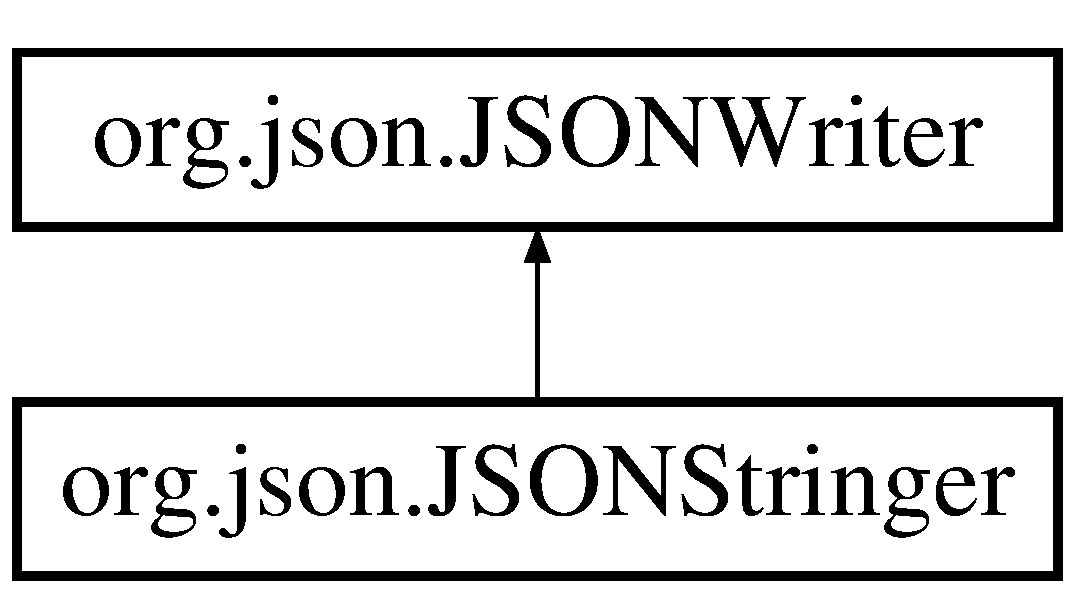
\includegraphics[height=2.000000cm]{classorg_1_1json_1_1_j_s_o_n_writer}
\end{center}
\end{figure}
\subsection*{Public Member Functions}
\begin{DoxyCompactItemize}
\item 
\hyperlink{classorg_1_1json_1_1_j_s_o_n_writer_a312dcf78fa8b46635043eb6b06184d5b}{J\-S\-O\-N\-Writer} (Writer w)
\item 
\hyperlink{classorg_1_1json_1_1_j_s_o_n_writer}{J\-S\-O\-N\-Writer} \hyperlink{classorg_1_1json_1_1_j_s_o_n_writer_aed48f7396fd364c0bc4f08b51f31afc4}{array} ()  throws J\-S\-O\-N\-Exception 
\item 
\hyperlink{classorg_1_1json_1_1_j_s_o_n_writer}{J\-S\-O\-N\-Writer} \hyperlink{classorg_1_1json_1_1_j_s_o_n_writer_a9d310d7ccc581cc070771126ee063ffe}{end\-Array} ()  throws J\-S\-O\-N\-Exception 
\item 
\hyperlink{classorg_1_1json_1_1_j_s_o_n_writer}{J\-S\-O\-N\-Writer} \hyperlink{classorg_1_1json_1_1_j_s_o_n_writer_a25cc931ef86998c61f08b1d5eff22146}{end\-Object} ()  throws J\-S\-O\-N\-Exception 
\item 
\hyperlink{classorg_1_1json_1_1_j_s_o_n_writer}{J\-S\-O\-N\-Writer} \hyperlink{classorg_1_1json_1_1_j_s_o_n_writer_ab03474f521f6fc4d8cb15d2c129fb435}{key} (String string)  throws J\-S\-O\-N\-Exception 
\item 
\hyperlink{classorg_1_1json_1_1_j_s_o_n_writer}{J\-S\-O\-N\-Writer} \hyperlink{classorg_1_1json_1_1_j_s_o_n_writer_a50ed212b9c8c9f6a57c3ddfc6bf3126a}{object} ()  throws J\-S\-O\-N\-Exception 
\item 
\hyperlink{classorg_1_1json_1_1_j_s_o_n_writer}{J\-S\-O\-N\-Writer} \hyperlink{classorg_1_1json_1_1_j_s_o_n_writer_a29441174afee5fde940c973d20e056a9}{value} (boolean b)  throws J\-S\-O\-N\-Exception 
\item 
\hyperlink{classorg_1_1json_1_1_j_s_o_n_writer}{J\-S\-O\-N\-Writer} \hyperlink{classorg_1_1json_1_1_j_s_o_n_writer_a0d9da178cbec36fc9b6e89e1d840c882}{value} (double d)  throws J\-S\-O\-N\-Exception 
\item 
\hyperlink{classorg_1_1json_1_1_j_s_o_n_writer}{J\-S\-O\-N\-Writer} \hyperlink{classorg_1_1json_1_1_j_s_o_n_writer_a5f8bdc612c2629b41420ef8e0ea94a40}{value} (long l)  throws J\-S\-O\-N\-Exception 
\item 
\hyperlink{classorg_1_1json_1_1_j_s_o_n_writer}{J\-S\-O\-N\-Writer} \hyperlink{classorg_1_1json_1_1_j_s_o_n_writer_aeab2dfdffed2e034f8598be9c89d4be1}{value} (Object \hyperlink{classorg_1_1json_1_1_j_s_o_n_writer_a50ed212b9c8c9f6a57c3ddfc6bf3126a}{object})  throws J\-S\-O\-N\-Exception 
\end{DoxyCompactItemize}
\subsection*{Protected Attributes}
\begin{DoxyCompactItemize}
\item 
char \hyperlink{classorg_1_1json_1_1_j_s_o_n_writer_acabe6b245b148eabfaa3cf975f98073f}{mode}
\item 
Writer \hyperlink{classorg_1_1json_1_1_j_s_o_n_writer_ae5398a9b83a17ab31c993c52fc1c8e06}{writer}
\end{DoxyCompactItemize}
\subsection*{Private Member Functions}
\begin{DoxyCompactItemize}
\item 
\hyperlink{classorg_1_1json_1_1_j_s_o_n_writer}{J\-S\-O\-N\-Writer} \hyperlink{classorg_1_1json_1_1_j_s_o_n_writer_a68cca8bb48159b1cb6b3ca10b70d837e}{append} (String string)  throws J\-S\-O\-N\-Exception 
\item 
\hyperlink{classorg_1_1json_1_1_j_s_o_n_writer}{J\-S\-O\-N\-Writer} \hyperlink{classorg_1_1json_1_1_j_s_o_n_writer_ad858ebf7b9b5cb50288ed4c2f6882614}{end} (char \hyperlink{classorg_1_1json_1_1_j_s_o_n_writer_acabe6b245b148eabfaa3cf975f98073f}{mode}, char c)  throws J\-S\-O\-N\-Exception 
\item 
void \hyperlink{classorg_1_1json_1_1_j_s_o_n_writer_a7c0de62466d96075b112f921c588d462}{pop} (char c)  throws J\-S\-O\-N\-Exception 
\item 
void \hyperlink{classorg_1_1json_1_1_j_s_o_n_writer_af52fc5a46190837106c20d17dd58d2f5}{push} (\hyperlink{classorg_1_1json_1_1_j_s_o_n_object}{J\-S\-O\-N\-Object} jo)  throws J\-S\-O\-N\-Exception 
\end{DoxyCompactItemize}
\subsection*{Private Attributes}
\begin{DoxyCompactItemize}
\item 
boolean \hyperlink{classorg_1_1json_1_1_j_s_o_n_writer_a2370b9e0c4400cc324ba5fb32a1ed311}{comma}
\item 
final \hyperlink{classorg_1_1json_1_1_j_s_o_n_object}{J\-S\-O\-N\-Object} \hyperlink{classorg_1_1json_1_1_j_s_o_n_writer_a06c3b64f8f98ba2bb2a3f57b1c5b328f}{stack} \mbox{[}$\,$\mbox{]}
\item 
int \hyperlink{classorg_1_1json_1_1_j_s_o_n_writer_a2da85e29823056f58034b8723b7da082}{top}
\end{DoxyCompactItemize}
\subsection*{Static Private Attributes}
\begin{DoxyCompactItemize}
\item 
static final int \hyperlink{classorg_1_1json_1_1_j_s_o_n_writer_a91e980e27ba1a1130621393aa245491a}{maxdepth} = 200
\end{DoxyCompactItemize}


\subsection{Detailed Description}
\hyperlink{classorg_1_1json_1_1_j_s_o_n_writer}{J\-S\-O\-N\-Writer} provides a quick and convenient way of producing J\-S\-O\-N text. The texts produced strictly conform to J\-S\-O\-N syntax rules. No whitespace is added, so the results are ready for transmission or storage. Each instance of \hyperlink{classorg_1_1json_1_1_j_s_o_n_writer}{J\-S\-O\-N\-Writer} can produce one J\-S\-O\-N text. 

A \hyperlink{classorg_1_1json_1_1_j_s_o_n_writer}{J\-S\-O\-N\-Writer} instance provides a {\ttfamily value} method for appending values to the text, and a {\ttfamily key} method for adding keys before values in objects. There are {\ttfamily array} and {\ttfamily end\-Array} methods that make and bound array values, and {\ttfamily object} and {\ttfamily end\-Object} methods which make and bound object values. All of these methods return the \hyperlink{classorg_1_1json_1_1_j_s_o_n_writer}{J\-S\-O\-N\-Writer} instance, permitting a cascade style. For example, 
\begin{DoxyPre}
new JSONWriter(myWriter)
    .\hyperlink{classorg_1_1json_1_1_j_s_o_n_writer_a50ed212b9c8c9f6a57c3ddfc6bf3126a}{object()}
        .key("JSON")
        .value("Hello, World!")
    .\hyperlink{classorg_1_1json_1_1_j_s_o_n_writer_a25cc931ef86998c61f08b1d5eff22146}{endObject()};\end{DoxyPre}
 which writes 
\begin{DoxyPre}
\{"JSON":"Hello, World!"\}\end{DoxyPre}
 

The first method called must be {\ttfamily array} or {\ttfamily object}. There are no methods for adding commas or colons. \hyperlink{classorg_1_1json_1_1_j_s_o_n_writer}{J\-S\-O\-N\-Writer} adds them for you. Objects and arrays can be nested up to 20 levels deep. 

This can sometimes be easier than using a \hyperlink{classorg_1_1json_1_1_j_s_o_n_object}{J\-S\-O\-N\-Object} to build a string. \begin{DoxyAuthor}{Author}
J\-S\-O\-N.\-org 
\end{DoxyAuthor}
\begin{DoxyVersion}{Version}
2011-\/11-\/24 
\end{DoxyVersion}


Definition at line 59 of file J\-S\-O\-N\-Writer.\-java.



\subsection{Constructor \& Destructor Documentation}
\hypertarget{classorg_1_1json_1_1_j_s_o_n_writer_a312dcf78fa8b46635043eb6b06184d5b}{\index{org\-::json\-::\-J\-S\-O\-N\-Writer@{org\-::json\-::\-J\-S\-O\-N\-Writer}!J\-S\-O\-N\-Writer@{J\-S\-O\-N\-Writer}}
\index{J\-S\-O\-N\-Writer@{J\-S\-O\-N\-Writer}!org::json::JSONWriter@{org\-::json\-::\-J\-S\-O\-N\-Writer}}
\subsubsection[{J\-S\-O\-N\-Writer}]{\setlength{\rightskip}{0pt plus 5cm}org.\-json.\-J\-S\-O\-N\-Writer.\-J\-S\-O\-N\-Writer (
\begin{DoxyParamCaption}
\item[{Writer}]{w}
\end{DoxyParamCaption}
)}}\label{classorg_1_1json_1_1_j_s_o_n_writer_a312dcf78fa8b46635043eb6b06184d5b}
Make a fresh \hyperlink{classorg_1_1json_1_1_j_s_o_n_writer}{J\-S\-O\-N\-Writer}. It can be used to build one J\-S\-O\-N text. 

Definition at line 96 of file J\-S\-O\-N\-Writer.\-java.



References org.\-json.\-J\-S\-O\-N\-Writer.\-comma, org.\-json.\-J\-S\-O\-N\-Writer.\-maxdepth, org.\-json.\-J\-S\-O\-N\-Writer.\-mode, org.\-json.\-J\-S\-O\-N\-Writer.\-stack, org.\-json.\-J\-S\-O\-N\-Writer.\-top, and org.\-json.\-J\-S\-O\-N\-Writer.\-writer.


\begin{DoxyCode}
96                                 \{
97         this.\hyperlink{classorg_1_1json_1_1_j_s_o_n_writer_a2370b9e0c4400cc324ba5fb32a1ed311}{comma} = \textcolor{keyword}{false};
98         this.\hyperlink{classorg_1_1json_1_1_j_s_o_n_writer_acabe6b245b148eabfaa3cf975f98073f}{mode} = \textcolor{charliteral}{'i'};
99         this.\hyperlink{classorg_1_1json_1_1_j_s_o_n_writer_a06c3b64f8f98ba2bb2a3f57b1c5b328f}{stack} = \textcolor{keyword}{new} JSONObject[\hyperlink{classorg_1_1json_1_1_j_s_o_n_writer_a91e980e27ba1a1130621393aa245491a}{maxdepth}];
100         this.\hyperlink{classorg_1_1json_1_1_j_s_o_n_writer_a2da85e29823056f58034b8723b7da082}{top} = 0;
101         this.\hyperlink{classorg_1_1json_1_1_j_s_o_n_writer_ae5398a9b83a17ab31c993c52fc1c8e06}{writer} = w;
102     \}
\end{DoxyCode}


\subsection{Member Function Documentation}
\hypertarget{classorg_1_1json_1_1_j_s_o_n_writer_a68cca8bb48159b1cb6b3ca10b70d837e}{\index{org\-::json\-::\-J\-S\-O\-N\-Writer@{org\-::json\-::\-J\-S\-O\-N\-Writer}!append@{append}}
\index{append@{append}!org::json::JSONWriter@{org\-::json\-::\-J\-S\-O\-N\-Writer}}
\subsubsection[{append}]{\setlength{\rightskip}{0pt plus 5cm}{\bf J\-S\-O\-N\-Writer} org.\-json.\-J\-S\-O\-N\-Writer.\-append (
\begin{DoxyParamCaption}
\item[{String}]{string}
\end{DoxyParamCaption}
) throws {\bf J\-S\-O\-N\-Exception}\hspace{0.3cm}{\ttfamily [private]}}}\label{classorg_1_1json_1_1_j_s_o_n_writer_a68cca8bb48159b1cb6b3ca10b70d837e}
Append a value. 
\begin{DoxyParams}{Parameters}
{\em string} & A string value. \\
\hline
\end{DoxyParams}
\begin{DoxyReturn}{Returns}
this 
\end{DoxyReturn}

\begin{DoxyExceptions}{Exceptions}
{\em \hyperlink{classorg_1_1json_1_1_j_s_o_n_exception}{J\-S\-O\-N\-Exception}} & If the value is out of sequence. \\
\hline
\end{DoxyExceptions}


Definition at line 110 of file J\-S\-O\-N\-Writer.\-java.



References org.\-json.\-J\-S\-O\-N\-Writer.\-comma, org.\-json.\-J\-S\-O\-N\-Writer.\-mode, and org.\-json.\-J\-S\-O\-N\-Writer.\-writer.



Referenced by org.\-json.\-J\-S\-O\-N\-Writer.\-array(), org.\-json.\-J\-S\-O\-N\-Writer.\-object(), and org.\-json.\-J\-S\-O\-N\-Writer.\-value().


\begin{DoxyCode}
110                                                                   \{
111         \textcolor{keywordflow}{if} (\textcolor{keywordtype}{string} == null) \{
112             \textcolor{keywordflow}{throw} \textcolor{keyword}{new} JSONException(\textcolor{stringliteral}{"Null pointer"});
113         \}
114         \textcolor{keywordflow}{if} (this.\hyperlink{classorg_1_1json_1_1_j_s_o_n_writer_acabe6b245b148eabfaa3cf975f98073f}{mode} == \textcolor{charliteral}{'o'} || this.\hyperlink{classorg_1_1json_1_1_j_s_o_n_writer_acabe6b245b148eabfaa3cf975f98073f}{mode} == \textcolor{charliteral}{'a'}) \{
115             \textcolor{keywordflow}{try} \{
116                 \textcolor{keywordflow}{if} (this.\hyperlink{classorg_1_1json_1_1_j_s_o_n_writer_a2370b9e0c4400cc324ba5fb32a1ed311}{comma} && this.\hyperlink{classorg_1_1json_1_1_j_s_o_n_writer_acabe6b245b148eabfaa3cf975f98073f}{mode} == \textcolor{charliteral}{'a'}) \{
117                     this.\hyperlink{classorg_1_1json_1_1_j_s_o_n_writer_ae5398a9b83a17ab31c993c52fc1c8e06}{writer}.write(\textcolor{charliteral}{','});
118                 \}
119                 this.\hyperlink{classorg_1_1json_1_1_j_s_o_n_writer_ae5398a9b83a17ab31c993c52fc1c8e06}{writer}.write(\textcolor{keywordtype}{string});
120             \} \textcolor{keywordflow}{catch} (IOException e) \{
121                 \textcolor{keywordflow}{throw} \textcolor{keyword}{new} JSONException(e);
122             \}
123             \textcolor{keywordflow}{if} (this.\hyperlink{classorg_1_1json_1_1_j_s_o_n_writer_acabe6b245b148eabfaa3cf975f98073f}{mode} == \textcolor{charliteral}{'o'}) \{
124                 this.\hyperlink{classorg_1_1json_1_1_j_s_o_n_writer_acabe6b245b148eabfaa3cf975f98073f}{mode} = \textcolor{charliteral}{'k'};
125             \}
126             this.\hyperlink{classorg_1_1json_1_1_j_s_o_n_writer_a2370b9e0c4400cc324ba5fb32a1ed311}{comma} = \textcolor{keyword}{true};
127             \textcolor{keywordflow}{return} \textcolor{keyword}{this};
128         \}
129         \textcolor{keywordflow}{throw} \textcolor{keyword}{new} JSONException(\textcolor{stringliteral}{"Value out of sequence."});
130     \}
\end{DoxyCode}
\hypertarget{classorg_1_1json_1_1_j_s_o_n_writer_aed48f7396fd364c0bc4f08b51f31afc4}{\index{org\-::json\-::\-J\-S\-O\-N\-Writer@{org\-::json\-::\-J\-S\-O\-N\-Writer}!array@{array}}
\index{array@{array}!org::json::JSONWriter@{org\-::json\-::\-J\-S\-O\-N\-Writer}}
\subsubsection[{array}]{\setlength{\rightskip}{0pt plus 5cm}{\bf J\-S\-O\-N\-Writer} org.\-json.\-J\-S\-O\-N\-Writer.\-array (
\begin{DoxyParamCaption}
{}
\end{DoxyParamCaption}
) throws {\bf J\-S\-O\-N\-Exception}}}\label{classorg_1_1json_1_1_j_s_o_n_writer_aed48f7396fd364c0bc4f08b51f31afc4}
Begin appending a new array. All values until the balancing {\ttfamily end\-Array} will be appended to this array. The {\ttfamily end\-Array} method must be called to mark the array's end. \begin{DoxyReturn}{Returns}
this 
\end{DoxyReturn}

\begin{DoxyExceptions}{Exceptions}
{\em \hyperlink{classorg_1_1json_1_1_j_s_o_n_exception}{J\-S\-O\-N\-Exception}} & If the nesting is too deep, or if the object is started in the wrong place (for example as a key or after the end of the outermost array or object). \\
\hline
\end{DoxyExceptions}


Definition at line 141 of file J\-S\-O\-N\-Writer.\-java.



References org.\-json.\-J\-S\-O\-N\-Writer.\-append(), org.\-json.\-J\-S\-O\-N\-Writer.\-comma, org.\-json.\-J\-S\-O\-N\-Writer.\-mode, and org.\-json.\-J\-S\-O\-N\-Writer.\-push().


\begin{DoxyCode}
141                                                    \{
142         \textcolor{keywordflow}{if} (this.\hyperlink{classorg_1_1json_1_1_j_s_o_n_writer_acabe6b245b148eabfaa3cf975f98073f}{mode} == \textcolor{charliteral}{'i'} || this.\hyperlink{classorg_1_1json_1_1_j_s_o_n_writer_acabe6b245b148eabfaa3cf975f98073f}{mode} == \textcolor{charliteral}{'o'} || this.\hyperlink{classorg_1_1json_1_1_j_s_o_n_writer_acabe6b245b148eabfaa3cf975f98073f}{mode} == \textcolor{charliteral}{'a'}) \{
143             this.\hyperlink{classorg_1_1json_1_1_j_s_o_n_writer_af52fc5a46190837106c20d17dd58d2f5}{push}(null);
144             this.\hyperlink{classorg_1_1json_1_1_j_s_o_n_writer_a68cca8bb48159b1cb6b3ca10b70d837e}{append}(\textcolor{stringliteral}{"["});
145             this.\hyperlink{classorg_1_1json_1_1_j_s_o_n_writer_a2370b9e0c4400cc324ba5fb32a1ed311}{comma} = \textcolor{keyword}{false};
146             \textcolor{keywordflow}{return} \textcolor{keyword}{this};
147         \}
148         \textcolor{keywordflow}{throw} \textcolor{keyword}{new} JSONException(\textcolor{stringliteral}{"Misplaced array."});
149     \}
\end{DoxyCode}
\hypertarget{classorg_1_1json_1_1_j_s_o_n_writer_ad858ebf7b9b5cb50288ed4c2f6882614}{\index{org\-::json\-::\-J\-S\-O\-N\-Writer@{org\-::json\-::\-J\-S\-O\-N\-Writer}!end@{end}}
\index{end@{end}!org::json::JSONWriter@{org\-::json\-::\-J\-S\-O\-N\-Writer}}
\subsubsection[{end}]{\setlength{\rightskip}{0pt plus 5cm}{\bf J\-S\-O\-N\-Writer} org.\-json.\-J\-S\-O\-N\-Writer.\-end (
\begin{DoxyParamCaption}
\item[{char}]{mode, }
\item[{char}]{c}
\end{DoxyParamCaption}
) throws {\bf J\-S\-O\-N\-Exception}\hspace{0.3cm}{\ttfamily [private]}}}\label{classorg_1_1json_1_1_j_s_o_n_writer_ad858ebf7b9b5cb50288ed4c2f6882614}
End something. 
\begin{DoxyParams}{Parameters}
{\em mode} & Mode \\
\hline
{\em c} & Closing character \\
\hline
\end{DoxyParams}
\begin{DoxyReturn}{Returns}
this 
\end{DoxyReturn}

\begin{DoxyExceptions}{Exceptions}
{\em \hyperlink{classorg_1_1json_1_1_j_s_o_n_exception}{J\-S\-O\-N\-Exception}} & If unbalanced. \\
\hline
\end{DoxyExceptions}


Definition at line 158 of file J\-S\-O\-N\-Writer.\-java.



References org.\-json.\-J\-S\-O\-N\-Writer.\-comma, org.\-json.\-J\-S\-O\-N\-Writer.\-mode, org.\-json.\-J\-S\-O\-N\-Writer.\-pop(), and org.\-json.\-J\-S\-O\-N\-Writer.\-writer.



Referenced by org.\-json.\-J\-S\-O\-N\-Writer.\-end\-Array(), and org.\-json.\-J\-S\-O\-N\-Writer.\-end\-Object().


\begin{DoxyCode}
158                                                                    \{
159         \textcolor{keywordflow}{if} (this.\hyperlink{classorg_1_1json_1_1_j_s_o_n_writer_acabe6b245b148eabfaa3cf975f98073f}{mode} != \hyperlink{classorg_1_1json_1_1_j_s_o_n_writer_acabe6b245b148eabfaa3cf975f98073f}{mode}) \{
160             \textcolor{keywordflow}{throw} \textcolor{keyword}{new} JSONException(\hyperlink{classorg_1_1json_1_1_j_s_o_n_writer_acabe6b245b148eabfaa3cf975f98073f}{mode} == \textcolor{charliteral}{'a'}
161                 ? \textcolor{stringliteral}{"Misplaced endArray."}
162                 : \textcolor{stringliteral}{"Misplaced endObject."});
163         \}
164         this.\hyperlink{classorg_1_1json_1_1_j_s_o_n_writer_a7c0de62466d96075b112f921c588d462}{pop}(\hyperlink{classorg_1_1json_1_1_j_s_o_n_writer_acabe6b245b148eabfaa3cf975f98073f}{mode});
165         \textcolor{keywordflow}{try} \{
166             this.\hyperlink{classorg_1_1json_1_1_j_s_o_n_writer_ae5398a9b83a17ab31c993c52fc1c8e06}{writer}.write(c);
167         \} \textcolor{keywordflow}{catch} (IOException e) \{
168             \textcolor{keywordflow}{throw} \textcolor{keyword}{new} JSONException(e);
169         \}
170         this.\hyperlink{classorg_1_1json_1_1_j_s_o_n_writer_a2370b9e0c4400cc324ba5fb32a1ed311}{comma} = \textcolor{keyword}{true};
171         \textcolor{keywordflow}{return} \textcolor{keyword}{this};
172     \}
\end{DoxyCode}
\hypertarget{classorg_1_1json_1_1_j_s_o_n_writer_a9d310d7ccc581cc070771126ee063ffe}{\index{org\-::json\-::\-J\-S\-O\-N\-Writer@{org\-::json\-::\-J\-S\-O\-N\-Writer}!end\-Array@{end\-Array}}
\index{end\-Array@{end\-Array}!org::json::JSONWriter@{org\-::json\-::\-J\-S\-O\-N\-Writer}}
\subsubsection[{end\-Array}]{\setlength{\rightskip}{0pt plus 5cm}{\bf J\-S\-O\-N\-Writer} org.\-json.\-J\-S\-O\-N\-Writer.\-end\-Array (
\begin{DoxyParamCaption}
{}
\end{DoxyParamCaption}
) throws {\bf J\-S\-O\-N\-Exception}}}\label{classorg_1_1json_1_1_j_s_o_n_writer_a9d310d7ccc581cc070771126ee063ffe}
End an array. This method most be called to balance calls to {\ttfamily array}. \begin{DoxyReturn}{Returns}
this 
\end{DoxyReturn}

\begin{DoxyExceptions}{Exceptions}
{\em \hyperlink{classorg_1_1json_1_1_j_s_o_n_exception}{J\-S\-O\-N\-Exception}} & If incorrectly nested. \\
\hline
\end{DoxyExceptions}


Definition at line 180 of file J\-S\-O\-N\-Writer.\-java.



References org.\-json.\-J\-S\-O\-N\-Writer.\-end().


\begin{DoxyCode}
180                                                       \{
181         \textcolor{keywordflow}{return} this.\hyperlink{classorg_1_1json_1_1_j_s_o_n_writer_ad858ebf7b9b5cb50288ed4c2f6882614}{end}(\textcolor{charliteral}{'a'}, \textcolor{charliteral}{']'});
182     \}
\end{DoxyCode}
\hypertarget{classorg_1_1json_1_1_j_s_o_n_writer_a25cc931ef86998c61f08b1d5eff22146}{\index{org\-::json\-::\-J\-S\-O\-N\-Writer@{org\-::json\-::\-J\-S\-O\-N\-Writer}!end\-Object@{end\-Object}}
\index{end\-Object@{end\-Object}!org::json::JSONWriter@{org\-::json\-::\-J\-S\-O\-N\-Writer}}
\subsubsection[{end\-Object}]{\setlength{\rightskip}{0pt plus 5cm}{\bf J\-S\-O\-N\-Writer} org.\-json.\-J\-S\-O\-N\-Writer.\-end\-Object (
\begin{DoxyParamCaption}
{}
\end{DoxyParamCaption}
) throws {\bf J\-S\-O\-N\-Exception}}}\label{classorg_1_1json_1_1_j_s_o_n_writer_a25cc931ef86998c61f08b1d5eff22146}
End an object. This method most be called to balance calls to {\ttfamily object}. \begin{DoxyReturn}{Returns}
this 
\end{DoxyReturn}

\begin{DoxyExceptions}{Exceptions}
{\em \hyperlink{classorg_1_1json_1_1_j_s_o_n_exception}{J\-S\-O\-N\-Exception}} & If incorrectly nested. \\
\hline
\end{DoxyExceptions}


Definition at line 190 of file J\-S\-O\-N\-Writer.\-java.



References org.\-json.\-J\-S\-O\-N\-Writer.\-end().


\begin{DoxyCode}
190                                                        \{
191         \textcolor{keywordflow}{return} this.\hyperlink{classorg_1_1json_1_1_j_s_o_n_writer_ad858ebf7b9b5cb50288ed4c2f6882614}{end}(\textcolor{charliteral}{'k'}, \textcolor{charliteral}{'\}'});
192     \}
\end{DoxyCode}
\hypertarget{classorg_1_1json_1_1_j_s_o_n_writer_ab03474f521f6fc4d8cb15d2c129fb435}{\index{org\-::json\-::\-J\-S\-O\-N\-Writer@{org\-::json\-::\-J\-S\-O\-N\-Writer}!key@{key}}
\index{key@{key}!org::json::JSONWriter@{org\-::json\-::\-J\-S\-O\-N\-Writer}}
\subsubsection[{key}]{\setlength{\rightskip}{0pt plus 5cm}{\bf J\-S\-O\-N\-Writer} org.\-json.\-J\-S\-O\-N\-Writer.\-key (
\begin{DoxyParamCaption}
\item[{String}]{string}
\end{DoxyParamCaption}
) throws {\bf J\-S\-O\-N\-Exception}}}\label{classorg_1_1json_1_1_j_s_o_n_writer_ab03474f521f6fc4d8cb15d2c129fb435}
Append a key. The key will be associated with the next value. In an object, every value must be preceded by a key. 
\begin{DoxyParams}{Parameters}
{\em string} & A key string. \\
\hline
\end{DoxyParams}
\begin{DoxyReturn}{Returns}
this 
\end{DoxyReturn}

\begin{DoxyExceptions}{Exceptions}
{\em \hyperlink{classorg_1_1json_1_1_j_s_o_n_exception}{J\-S\-O\-N\-Exception}} & If the key is out of place. For example, keys do not belong in arrays or if the key is null. \\
\hline
\end{DoxyExceptions}


Definition at line 202 of file J\-S\-O\-N\-Writer.\-java.



References org.\-json.\-J\-S\-O\-N\-Writer.\-comma, org.\-json.\-J\-S\-O\-N\-Writer.\-mode, org.\-json.\-J\-S\-O\-N\-Object.\-put\-Once(), org.\-json.\-J\-S\-O\-N\-Object.\-quote(), org.\-json.\-J\-S\-O\-N\-Writer.\-stack, org.\-json.\-J\-S\-O\-N\-Writer.\-top, and org.\-json.\-J\-S\-O\-N\-Writer.\-writer.


\begin{DoxyCode}
202                                                               \{
203         \textcolor{keywordflow}{if} (\textcolor{keywordtype}{string} == null) \{
204             \textcolor{keywordflow}{throw} \textcolor{keyword}{new} JSONException(\textcolor{stringliteral}{"Null key."});
205         \}
206         \textcolor{keywordflow}{if} (this.\hyperlink{classorg_1_1json_1_1_j_s_o_n_writer_acabe6b245b148eabfaa3cf975f98073f}{mode} == \textcolor{charliteral}{'k'}) \{
207             \textcolor{keywordflow}{try} \{
208                 this.\hyperlink{classorg_1_1json_1_1_j_s_o_n_writer_a06c3b64f8f98ba2bb2a3f57b1c5b328f}{stack}[this.\hyperlink{classorg_1_1json_1_1_j_s_o_n_writer_a2da85e29823056f58034b8723b7da082}{top} - 1].\hyperlink{classorg_1_1json_1_1_j_s_o_n_object_ac6cc7fe095a7711be90f2e02163ef49e}{putOnce}(\textcolor{keywordtype}{string}, Boolean.TRUE);
209                 \textcolor{keywordflow}{if} (this.\hyperlink{classorg_1_1json_1_1_j_s_o_n_writer_a2370b9e0c4400cc324ba5fb32a1ed311}{comma}) \{
210                     this.\hyperlink{classorg_1_1json_1_1_j_s_o_n_writer_ae5398a9b83a17ab31c993c52fc1c8e06}{writer}.write(\textcolor{charliteral}{','});
211                 \}
212                 this.\hyperlink{classorg_1_1json_1_1_j_s_o_n_writer_ae5398a9b83a17ab31c993c52fc1c8e06}{writer}.write(JSONObject.quote(\textcolor{keywordtype}{string}));
213                 this.\hyperlink{classorg_1_1json_1_1_j_s_o_n_writer_ae5398a9b83a17ab31c993c52fc1c8e06}{writer}.write(\textcolor{charliteral}{':'});
214                 this.\hyperlink{classorg_1_1json_1_1_j_s_o_n_writer_a2370b9e0c4400cc324ba5fb32a1ed311}{comma} = \textcolor{keyword}{false};
215                 this.\hyperlink{classorg_1_1json_1_1_j_s_o_n_writer_acabe6b245b148eabfaa3cf975f98073f}{mode} = \textcolor{charliteral}{'o'};
216                 \textcolor{keywordflow}{return} \textcolor{keyword}{this};
217             \} \textcolor{keywordflow}{catch} (IOException e) \{
218                 \textcolor{keywordflow}{throw} \textcolor{keyword}{new} JSONException(e);
219             \}
220         \}
221         \textcolor{keywordflow}{throw} \textcolor{keyword}{new} JSONException(\textcolor{stringliteral}{"Misplaced key."});
222     \}
\end{DoxyCode}
\hypertarget{classorg_1_1json_1_1_j_s_o_n_writer_a50ed212b9c8c9f6a57c3ddfc6bf3126a}{\index{org\-::json\-::\-J\-S\-O\-N\-Writer@{org\-::json\-::\-J\-S\-O\-N\-Writer}!object@{object}}
\index{object@{object}!org::json::JSONWriter@{org\-::json\-::\-J\-S\-O\-N\-Writer}}
\subsubsection[{object}]{\setlength{\rightskip}{0pt plus 5cm}{\bf J\-S\-O\-N\-Writer} org.\-json.\-J\-S\-O\-N\-Writer.\-object (
\begin{DoxyParamCaption}
{}
\end{DoxyParamCaption}
) throws {\bf J\-S\-O\-N\-Exception}}}\label{classorg_1_1json_1_1_j_s_o_n_writer_a50ed212b9c8c9f6a57c3ddfc6bf3126a}
Begin appending a new object. All keys and values until the balancing {\ttfamily end\-Object} will be appended to this object. The {\ttfamily end\-Object} method must be called to mark the object's end. \begin{DoxyReturn}{Returns}
this 
\end{DoxyReturn}

\begin{DoxyExceptions}{Exceptions}
{\em \hyperlink{classorg_1_1json_1_1_j_s_o_n_exception}{J\-S\-O\-N\-Exception}} & If the nesting is too deep, or if the object is started in the wrong place (for example as a key or after the end of the outermost array or object). \\
\hline
\end{DoxyExceptions}


Definition at line 234 of file J\-S\-O\-N\-Writer.\-java.



References org.\-json.\-J\-S\-O\-N\-Writer.\-append(), org.\-json.\-J\-S\-O\-N\-Writer.\-comma, org.\-json.\-J\-S\-O\-N\-Writer.\-mode, and org.\-json.\-J\-S\-O\-N\-Writer.\-push().


\begin{DoxyCode}
234                                                     \{
235         \textcolor{keywordflow}{if} (this.\hyperlink{classorg_1_1json_1_1_j_s_o_n_writer_acabe6b245b148eabfaa3cf975f98073f}{mode} == \textcolor{charliteral}{'i'}) \{
236             this.\hyperlink{classorg_1_1json_1_1_j_s_o_n_writer_acabe6b245b148eabfaa3cf975f98073f}{mode} = \textcolor{charliteral}{'o'};
237         \}
238         \textcolor{keywordflow}{if} (this.\hyperlink{classorg_1_1json_1_1_j_s_o_n_writer_acabe6b245b148eabfaa3cf975f98073f}{mode} == \textcolor{charliteral}{'o'} || this.\hyperlink{classorg_1_1json_1_1_j_s_o_n_writer_acabe6b245b148eabfaa3cf975f98073f}{mode} == \textcolor{charliteral}{'a'}) \{
239             this.\hyperlink{classorg_1_1json_1_1_j_s_o_n_writer_a68cca8bb48159b1cb6b3ca10b70d837e}{append}(\textcolor{stringliteral}{"\{"});
240             this.\hyperlink{classorg_1_1json_1_1_j_s_o_n_writer_af52fc5a46190837106c20d17dd58d2f5}{push}(\textcolor{keyword}{new} JSONObject());
241             this.\hyperlink{classorg_1_1json_1_1_j_s_o_n_writer_a2370b9e0c4400cc324ba5fb32a1ed311}{comma} = \textcolor{keyword}{false};
242             \textcolor{keywordflow}{return} \textcolor{keyword}{this};
243         \}
244         \textcolor{keywordflow}{throw} \textcolor{keyword}{new} JSONException(\textcolor{stringliteral}{"Misplaced object."});
245 
246     \}
\end{DoxyCode}
\hypertarget{classorg_1_1json_1_1_j_s_o_n_writer_a7c0de62466d96075b112f921c588d462}{\index{org\-::json\-::\-J\-S\-O\-N\-Writer@{org\-::json\-::\-J\-S\-O\-N\-Writer}!pop@{pop}}
\index{pop@{pop}!org::json::JSONWriter@{org\-::json\-::\-J\-S\-O\-N\-Writer}}
\subsubsection[{pop}]{\setlength{\rightskip}{0pt plus 5cm}void org.\-json.\-J\-S\-O\-N\-Writer.\-pop (
\begin{DoxyParamCaption}
\item[{char}]{c}
\end{DoxyParamCaption}
) throws {\bf J\-S\-O\-N\-Exception}\hspace{0.3cm}{\ttfamily [private]}}}\label{classorg_1_1json_1_1_j_s_o_n_writer_a7c0de62466d96075b112f921c588d462}
Pop an array or object scope. 
\begin{DoxyParams}{Parameters}
{\em c} & The scope to close. \\
\hline
\end{DoxyParams}

\begin{DoxyExceptions}{Exceptions}
{\em \hyperlink{classorg_1_1json_1_1_j_s_o_n_exception}{J\-S\-O\-N\-Exception}} & If nesting is wrong. \\
\hline
\end{DoxyExceptions}


Definition at line 254 of file J\-S\-O\-N\-Writer.\-java.



References org.\-json.\-J\-S\-O\-N\-Writer.\-mode, org.\-json.\-J\-S\-O\-N\-Writer.\-stack, and org.\-json.\-J\-S\-O\-N\-Writer.\-top.



Referenced by org.\-json.\-J\-S\-O\-N\-Writer.\-end().


\begin{DoxyCode}
254                                                   \{
255         \textcolor{keywordflow}{if} (this.\hyperlink{classorg_1_1json_1_1_j_s_o_n_writer_a2da85e29823056f58034b8723b7da082}{top} <= 0) \{
256             \textcolor{keywordflow}{throw} \textcolor{keyword}{new} JSONException(\textcolor{stringliteral}{"Nesting error."});
257         \}
258         \textcolor{keywordtype}{char} m = this.\hyperlink{classorg_1_1json_1_1_j_s_o_n_writer_a06c3b64f8f98ba2bb2a3f57b1c5b328f}{stack}[this.\hyperlink{classorg_1_1json_1_1_j_s_o_n_writer_a2da85e29823056f58034b8723b7da082}{top} - 1] == null ? \textcolor{charliteral}{'a'} : \textcolor{charliteral}{'k'};
259         \textcolor{keywordflow}{if} (m != c) \{
260             \textcolor{keywordflow}{throw} \textcolor{keyword}{new} JSONException(\textcolor{stringliteral}{"Nesting error."});
261         \}
262         this.\hyperlink{classorg_1_1json_1_1_j_s_o_n_writer_a2da85e29823056f58034b8723b7da082}{top} -= 1;
263         this.\hyperlink{classorg_1_1json_1_1_j_s_o_n_writer_acabe6b245b148eabfaa3cf975f98073f}{mode} = this.\hyperlink{classorg_1_1json_1_1_j_s_o_n_writer_a2da85e29823056f58034b8723b7da082}{top} == 0
264             ? \textcolor{charliteral}{'d'}
265             : this.\hyperlink{classorg_1_1json_1_1_j_s_o_n_writer_a06c3b64f8f98ba2bb2a3f57b1c5b328f}{stack}[this.\hyperlink{classorg_1_1json_1_1_j_s_o_n_writer_a2da85e29823056f58034b8723b7da082}{top} - 1] == null
266             ? \textcolor{charliteral}{'a'}
267             : \textcolor{charliteral}{'k'};
268     \}
\end{DoxyCode}
\hypertarget{classorg_1_1json_1_1_j_s_o_n_writer_af52fc5a46190837106c20d17dd58d2f5}{\index{org\-::json\-::\-J\-S\-O\-N\-Writer@{org\-::json\-::\-J\-S\-O\-N\-Writer}!push@{push}}
\index{push@{push}!org::json::JSONWriter@{org\-::json\-::\-J\-S\-O\-N\-Writer}}
\subsubsection[{push}]{\setlength{\rightskip}{0pt plus 5cm}void org.\-json.\-J\-S\-O\-N\-Writer.\-push (
\begin{DoxyParamCaption}
\item[{{\bf J\-S\-O\-N\-Object}}]{jo}
\end{DoxyParamCaption}
) throws {\bf J\-S\-O\-N\-Exception}\hspace{0.3cm}{\ttfamily [private]}}}\label{classorg_1_1json_1_1_j_s_o_n_writer_af52fc5a46190837106c20d17dd58d2f5}
Push an array or object scope. 
\begin{DoxyParams}{Parameters}
{\em c} & The scope to open. \\
\hline
\end{DoxyParams}

\begin{DoxyExceptions}{Exceptions}
{\em \hyperlink{classorg_1_1json_1_1_j_s_o_n_exception}{J\-S\-O\-N\-Exception}} & If nesting is too deep. \\
\hline
\end{DoxyExceptions}


Definition at line 275 of file J\-S\-O\-N\-Writer.\-java.



References org.\-json.\-J\-S\-O\-N\-Writer.\-maxdepth, org.\-json.\-J\-S\-O\-N\-Writer.\-mode, org.\-json.\-J\-S\-O\-N\-Writer.\-stack, and org.\-json.\-J\-S\-O\-N\-Writer.\-top.



Referenced by org.\-json.\-J\-S\-O\-N\-Writer.\-array(), and org.\-json.\-J\-S\-O\-N\-Writer.\-object().


\begin{DoxyCode}
275                                                           \{
276         \textcolor{keywordflow}{if} (this.\hyperlink{classorg_1_1json_1_1_j_s_o_n_writer_a2da85e29823056f58034b8723b7da082}{top} >= \hyperlink{classorg_1_1json_1_1_j_s_o_n_writer_a91e980e27ba1a1130621393aa245491a}{maxdepth}) \{
277             \textcolor{keywordflow}{throw} \textcolor{keyword}{new} JSONException(\textcolor{stringliteral}{"Nesting too deep."});
278         \}
279         this.\hyperlink{classorg_1_1json_1_1_j_s_o_n_writer_a06c3b64f8f98ba2bb2a3f57b1c5b328f}{stack}[this.\hyperlink{classorg_1_1json_1_1_j_s_o_n_writer_a2da85e29823056f58034b8723b7da082}{top}] = jo;
280         this.\hyperlink{classorg_1_1json_1_1_j_s_o_n_writer_acabe6b245b148eabfaa3cf975f98073f}{mode} = jo == null ? \textcolor{charliteral}{'a'} : \textcolor{charliteral}{'k'};
281         this.\hyperlink{classorg_1_1json_1_1_j_s_o_n_writer_a2da85e29823056f58034b8723b7da082}{top} += 1;
282     \}
\end{DoxyCode}
\hypertarget{classorg_1_1json_1_1_j_s_o_n_writer_a29441174afee5fde940c973d20e056a9}{\index{org\-::json\-::\-J\-S\-O\-N\-Writer@{org\-::json\-::\-J\-S\-O\-N\-Writer}!value@{value}}
\index{value@{value}!org::json::JSONWriter@{org\-::json\-::\-J\-S\-O\-N\-Writer}}
\subsubsection[{value}]{\setlength{\rightskip}{0pt plus 5cm}{\bf J\-S\-O\-N\-Writer} org.\-json.\-J\-S\-O\-N\-Writer.\-value (
\begin{DoxyParamCaption}
\item[{boolean}]{b}
\end{DoxyParamCaption}
) throws {\bf J\-S\-O\-N\-Exception}}}\label{classorg_1_1json_1_1_j_s_o_n_writer_a29441174afee5fde940c973d20e056a9}
Append either the value {\ttfamily true} or the value {\ttfamily false}. 
\begin{DoxyParams}{Parameters}
{\em b} & A boolean. \\
\hline
\end{DoxyParams}
\begin{DoxyReturn}{Returns}
this 
\end{DoxyReturn}

\begin{DoxyExceptions}{Exceptions}
{\em \hyperlink{classorg_1_1json_1_1_j_s_o_n_exception}{J\-S\-O\-N\-Exception}} & \\
\hline
\end{DoxyExceptions}


Definition at line 292 of file J\-S\-O\-N\-Writer.\-java.



References org.\-json.\-J\-S\-O\-N\-Writer.\-append().



Referenced by org.\-json.\-J\-S\-O\-N\-Writer.\-value().


\begin{DoxyCode}
292                                                             \{
293         \textcolor{keywordflow}{return} this.\hyperlink{classorg_1_1json_1_1_j_s_o_n_writer_a68cca8bb48159b1cb6b3ca10b70d837e}{append}(b ? \textcolor{stringliteral}{"true"} : \textcolor{stringliteral}{"false"});
294     \}
\end{DoxyCode}
\hypertarget{classorg_1_1json_1_1_j_s_o_n_writer_a0d9da178cbec36fc9b6e89e1d840c882}{\index{org\-::json\-::\-J\-S\-O\-N\-Writer@{org\-::json\-::\-J\-S\-O\-N\-Writer}!value@{value}}
\index{value@{value}!org::json::JSONWriter@{org\-::json\-::\-J\-S\-O\-N\-Writer}}
\subsubsection[{value}]{\setlength{\rightskip}{0pt plus 5cm}{\bf J\-S\-O\-N\-Writer} org.\-json.\-J\-S\-O\-N\-Writer.\-value (
\begin{DoxyParamCaption}
\item[{double}]{d}
\end{DoxyParamCaption}
) throws {\bf J\-S\-O\-N\-Exception}}}\label{classorg_1_1json_1_1_j_s_o_n_writer_a0d9da178cbec36fc9b6e89e1d840c882}
Append a double value. 
\begin{DoxyParams}{Parameters}
{\em d} & A double. \\
\hline
\end{DoxyParams}
\begin{DoxyReturn}{Returns}
this 
\end{DoxyReturn}

\begin{DoxyExceptions}{Exceptions}
{\em \hyperlink{classorg_1_1json_1_1_j_s_o_n_exception}{J\-S\-O\-N\-Exception}} & If the number is not finite. \\
\hline
\end{DoxyExceptions}


Definition at line 302 of file J\-S\-O\-N\-Writer.\-java.



References org.\-json.\-J\-S\-O\-N\-Writer.\-value().


\begin{DoxyCode}
302                                                            \{
303         \textcolor{keywordflow}{return} this.\hyperlink{classorg_1_1json_1_1_j_s_o_n_writer_a29441174afee5fde940c973d20e056a9}{value}(\textcolor{keyword}{new} Double(d));
304     \}
\end{DoxyCode}
\hypertarget{classorg_1_1json_1_1_j_s_o_n_writer_a5f8bdc612c2629b41420ef8e0ea94a40}{\index{org\-::json\-::\-J\-S\-O\-N\-Writer@{org\-::json\-::\-J\-S\-O\-N\-Writer}!value@{value}}
\index{value@{value}!org::json::JSONWriter@{org\-::json\-::\-J\-S\-O\-N\-Writer}}
\subsubsection[{value}]{\setlength{\rightskip}{0pt plus 5cm}{\bf J\-S\-O\-N\-Writer} org.\-json.\-J\-S\-O\-N\-Writer.\-value (
\begin{DoxyParamCaption}
\item[{long}]{l}
\end{DoxyParamCaption}
) throws {\bf J\-S\-O\-N\-Exception}}}\label{classorg_1_1json_1_1_j_s_o_n_writer_a5f8bdc612c2629b41420ef8e0ea94a40}
Append a long value. 
\begin{DoxyParams}{Parameters}
{\em l} & A long. \\
\hline
\end{DoxyParams}
\begin{DoxyReturn}{Returns}
this 
\end{DoxyReturn}

\begin{DoxyExceptions}{Exceptions}
{\em \hyperlink{classorg_1_1json_1_1_j_s_o_n_exception}{J\-S\-O\-N\-Exception}} & \\
\hline
\end{DoxyExceptions}


Definition at line 312 of file J\-S\-O\-N\-Writer.\-java.



References org.\-json.\-J\-S\-O\-N\-Writer.\-append().


\begin{DoxyCode}
312                                                          \{
313         \textcolor{keywordflow}{return} this.\hyperlink{classorg_1_1json_1_1_j_s_o_n_writer_a68cca8bb48159b1cb6b3ca10b70d837e}{append}(Long.toString(l));
314     \}
\end{DoxyCode}
\hypertarget{classorg_1_1json_1_1_j_s_o_n_writer_aeab2dfdffed2e034f8598be9c89d4be1}{\index{org\-::json\-::\-J\-S\-O\-N\-Writer@{org\-::json\-::\-J\-S\-O\-N\-Writer}!value@{value}}
\index{value@{value}!org::json::JSONWriter@{org\-::json\-::\-J\-S\-O\-N\-Writer}}
\subsubsection[{value}]{\setlength{\rightskip}{0pt plus 5cm}{\bf J\-S\-O\-N\-Writer} org.\-json.\-J\-S\-O\-N\-Writer.\-value (
\begin{DoxyParamCaption}
\item[{Object}]{object}
\end{DoxyParamCaption}
) throws {\bf J\-S\-O\-N\-Exception}}}\label{classorg_1_1json_1_1_j_s_o_n_writer_aeab2dfdffed2e034f8598be9c89d4be1}
Append an object value. 
\begin{DoxyParams}{Parameters}
{\em object} & The object to append. It can be null, or a Boolean, Number, String, \hyperlink{classorg_1_1json_1_1_j_s_o_n_object}{J\-S\-O\-N\-Object}, or \hyperlink{classorg_1_1json_1_1_j_s_o_n_array}{J\-S\-O\-N\-Array}, or an object that implements \hyperlink{interfaceorg_1_1json_1_1_j_s_o_n_string}{J\-S\-O\-N\-String}. \\
\hline
\end{DoxyParams}
\begin{DoxyReturn}{Returns}
this 
\end{DoxyReturn}

\begin{DoxyExceptions}{Exceptions}
{\em \hyperlink{classorg_1_1json_1_1_j_s_o_n_exception}{J\-S\-O\-N\-Exception}} & If the value is out of sequence. \\
\hline
\end{DoxyExceptions}


Definition at line 324 of file J\-S\-O\-N\-Writer.\-java.



References org.\-json.\-J\-S\-O\-N\-Writer.\-append(), and org.\-json.\-J\-S\-O\-N\-Object.\-value\-To\-String().


\begin{DoxyCode}
324                                                                 \{
325         \textcolor{keywordflow}{return} this.\hyperlink{classorg_1_1json_1_1_j_s_o_n_writer_a68cca8bb48159b1cb6b3ca10b70d837e}{append}(JSONObject.valueToString(\textcolor{keywordtype}{object}));
326     \}
\end{DoxyCode}


\subsection{Member Data Documentation}
\hypertarget{classorg_1_1json_1_1_j_s_o_n_writer_a2370b9e0c4400cc324ba5fb32a1ed311}{\index{org\-::json\-::\-J\-S\-O\-N\-Writer@{org\-::json\-::\-J\-S\-O\-N\-Writer}!comma@{comma}}
\index{comma@{comma}!org::json::JSONWriter@{org\-::json\-::\-J\-S\-O\-N\-Writer}}
\subsubsection[{comma}]{\setlength{\rightskip}{0pt plus 5cm}boolean org.\-json.\-J\-S\-O\-N\-Writer.\-comma\hspace{0.3cm}{\ttfamily [private]}}}\label{classorg_1_1json_1_1_j_s_o_n_writer_a2370b9e0c4400cc324ba5fb32a1ed311}
The comma flag determines if a comma should be output before the next value. 

Definition at line 66 of file J\-S\-O\-N\-Writer.\-java.



Referenced by org.\-json.\-J\-S\-O\-N\-Writer.\-append(), org.\-json.\-J\-S\-O\-N\-Writer.\-array(), org.\-json.\-J\-S\-O\-N\-Writer.\-end(), org.\-json.\-J\-S\-O\-N\-Writer.\-J\-S\-O\-N\-Writer(), org.\-json.\-J\-S\-O\-N\-Writer.\-key(), and org.\-json.\-J\-S\-O\-N\-Writer.\-object().

\hypertarget{classorg_1_1json_1_1_j_s_o_n_writer_a91e980e27ba1a1130621393aa245491a}{\index{org\-::json\-::\-J\-S\-O\-N\-Writer@{org\-::json\-::\-J\-S\-O\-N\-Writer}!maxdepth@{maxdepth}}
\index{maxdepth@{maxdepth}!org::json::JSONWriter@{org\-::json\-::\-J\-S\-O\-N\-Writer}}
\subsubsection[{maxdepth}]{\setlength{\rightskip}{0pt plus 5cm}final int org.\-json.\-J\-S\-O\-N\-Writer.\-maxdepth = 200\hspace{0.3cm}{\ttfamily [static]}, {\ttfamily [private]}}}\label{classorg_1_1json_1_1_j_s_o_n_writer_a91e980e27ba1a1130621393aa245491a}


Definition at line 60 of file J\-S\-O\-N\-Writer.\-java.



Referenced by org.\-json.\-J\-S\-O\-N\-Writer.\-J\-S\-O\-N\-Writer(), and org.\-json.\-J\-S\-O\-N\-Writer.\-push().

\hypertarget{classorg_1_1json_1_1_j_s_o_n_writer_acabe6b245b148eabfaa3cf975f98073f}{\index{org\-::json\-::\-J\-S\-O\-N\-Writer@{org\-::json\-::\-J\-S\-O\-N\-Writer}!mode@{mode}}
\index{mode@{mode}!org::json::JSONWriter@{org\-::json\-::\-J\-S\-O\-N\-Writer}}
\subsubsection[{mode}]{\setlength{\rightskip}{0pt plus 5cm}char org.\-json.\-J\-S\-O\-N\-Writer.\-mode\hspace{0.3cm}{\ttfamily [protected]}}}\label{classorg_1_1json_1_1_j_s_o_n_writer_acabe6b245b148eabfaa3cf975f98073f}
The current mode. Values\-: 'a' (array), 'd' (done), 'i' (initial), 'k' (key), 'o' (object). 

Definition at line 76 of file J\-S\-O\-N\-Writer.\-java.



Referenced by org.\-json.\-J\-S\-O\-N\-Writer.\-append(), org.\-json.\-J\-S\-O\-N\-Writer.\-array(), org.\-json.\-J\-S\-O\-N\-Writer.\-end(), org.\-json.\-J\-S\-O\-N\-Writer.\-J\-S\-O\-N\-Writer(), org.\-json.\-J\-S\-O\-N\-Writer.\-key(), org.\-json.\-J\-S\-O\-N\-Writer.\-object(), org.\-json.\-J\-S\-O\-N\-Writer.\-pop(), org.\-json.\-J\-S\-O\-N\-Writer.\-push(), and org.\-json.\-J\-S\-O\-N\-Stringer.\-to\-String().

\hypertarget{classorg_1_1json_1_1_j_s_o_n_writer_a06c3b64f8f98ba2bb2a3f57b1c5b328f}{\index{org\-::json\-::\-J\-S\-O\-N\-Writer@{org\-::json\-::\-J\-S\-O\-N\-Writer}!stack@{stack}}
\index{stack@{stack}!org::json::JSONWriter@{org\-::json\-::\-J\-S\-O\-N\-Writer}}
\subsubsection[{stack}]{\setlength{\rightskip}{0pt plus 5cm}final {\bf J\-S\-O\-N\-Object} org.\-json.\-J\-S\-O\-N\-Writer.\-stack\mbox{[}$\,$\mbox{]}\hspace{0.3cm}{\ttfamily [private]}}}\label{classorg_1_1json_1_1_j_s_o_n_writer_a06c3b64f8f98ba2bb2a3f57b1c5b328f}
The object/array stack. 

Definition at line 81 of file J\-S\-O\-N\-Writer.\-java.



Referenced by org.\-json.\-J\-S\-O\-N\-Writer.\-J\-S\-O\-N\-Writer(), org.\-json.\-J\-S\-O\-N\-Writer.\-key(), org.\-json.\-J\-S\-O\-N\-Writer.\-pop(), and org.\-json.\-J\-S\-O\-N\-Writer.\-push().

\hypertarget{classorg_1_1json_1_1_j_s_o_n_writer_a2da85e29823056f58034b8723b7da082}{\index{org\-::json\-::\-J\-S\-O\-N\-Writer@{org\-::json\-::\-J\-S\-O\-N\-Writer}!top@{top}}
\index{top@{top}!org::json::JSONWriter@{org\-::json\-::\-J\-S\-O\-N\-Writer}}
\subsubsection[{top}]{\setlength{\rightskip}{0pt plus 5cm}int org.\-json.\-J\-S\-O\-N\-Writer.\-top\hspace{0.3cm}{\ttfamily [private]}}}\label{classorg_1_1json_1_1_j_s_o_n_writer_a2da85e29823056f58034b8723b7da082}
The stack top index. A value of 0 indicates that the stack is empty. 

Definition at line 86 of file J\-S\-O\-N\-Writer.\-java.



Referenced by org.\-json.\-J\-S\-O\-N\-Writer.\-J\-S\-O\-N\-Writer(), org.\-json.\-J\-S\-O\-N\-Writer.\-key(), org.\-json.\-J\-S\-O\-N\-Writer.\-pop(), and org.\-json.\-J\-S\-O\-N\-Writer.\-push().

\hypertarget{classorg_1_1json_1_1_j_s_o_n_writer_ae5398a9b83a17ab31c993c52fc1c8e06}{\index{org\-::json\-::\-J\-S\-O\-N\-Writer@{org\-::json\-::\-J\-S\-O\-N\-Writer}!writer@{writer}}
\index{writer@{writer}!org::json::JSONWriter@{org\-::json\-::\-J\-S\-O\-N\-Writer}}
\subsubsection[{writer}]{\setlength{\rightskip}{0pt plus 5cm}Writer org.\-json.\-J\-S\-O\-N\-Writer.\-writer\hspace{0.3cm}{\ttfamily [protected]}}}\label{classorg_1_1json_1_1_j_s_o_n_writer_ae5398a9b83a17ab31c993c52fc1c8e06}
The writer that will receive the output. 

Definition at line 91 of file J\-S\-O\-N\-Writer.\-java.



Referenced by org.\-json.\-J\-S\-O\-N\-Writer.\-append(), org.\-json.\-J\-S\-O\-N\-Writer.\-end(), org.\-json.\-J\-S\-O\-N\-Writer.\-J\-S\-O\-N\-Writer(), org.\-json.\-J\-S\-O\-N\-Writer.\-key(), and org.\-json.\-J\-S\-O\-N\-Stringer.\-to\-String().



The documentation for this class was generated from the following file\-:\begin{DoxyCompactItemize}
\item 
org/json/\hyperlink{_j_s_o_n_writer_8java}{J\-S\-O\-N\-Writer.\-java}\end{DoxyCompactItemize}

\hypertarget{classorg_1_1json_1_1_kim}{\section{org.\-json.\-Kim Class Reference}
\label{classorg_1_1json_1_1_kim}\index{org.\-json.\-Kim@{org.\-json.\-Kim}}
}
\subsection*{Public Member Functions}
\begin{DoxyCompactItemize}
\item 
\hyperlink{classorg_1_1json_1_1_kim_a44b367e21f41746f63b7fc61c32ed259}{Kim} (byte\mbox{[}$\,$\mbox{]} \hyperlink{classorg_1_1json_1_1_kim_aca37e9b2f118afc91bc8d1f37512819b}{bytes}, int from, int thru)
\item 
\hyperlink{classorg_1_1json_1_1_kim_a397d63cbb42efcb488dd5fc6c7815fa1}{Kim} (byte\mbox{[}$\,$\mbox{]} \hyperlink{classorg_1_1json_1_1_kim_aca37e9b2f118afc91bc8d1f37512819b}{bytes}, int \hyperlink{classorg_1_1json_1_1_kim_a6caa186b493021e083e4efbf734e3a40}{length})
\item 
\hyperlink{classorg_1_1json_1_1_kim_a798dc70a0b04e45bf2afce778c7151c3}{Kim} (\hyperlink{classorg_1_1json_1_1_kim}{Kim} kim, int from, int thru)
\item 
\hyperlink{classorg_1_1json_1_1_kim_a652b4e6a919d52344c0e324348b577c4}{Kim} (String \hyperlink{classorg_1_1json_1_1_kim_ab3c21a745d0601eb36105ec3769a310a}{string})  throws J\-S\-O\-N\-Exception 
\item 
int \hyperlink{classorg_1_1json_1_1_kim_ac3c5fafa8f35357441582a217e2288ff}{character\-At} (int at)  throws J\-S\-O\-N\-Exception 
\item 
int \hyperlink{classorg_1_1json_1_1_kim_a2fee1848d7208b970312e02549323ef7}{copy} (byte\mbox{[}$\,$\mbox{]} \hyperlink{classorg_1_1json_1_1_kim_aca37e9b2f118afc91bc8d1f37512819b}{bytes}, int at)
\item 
boolean \hyperlink{classorg_1_1json_1_1_kim_a1ccd8538e3fa847b407f2192f54b71c4}{equals} (Object obj)
\item 
int \hyperlink{classorg_1_1json_1_1_kim_aef6fa7d8ec3cf6fc01858405479251d7}{get} (int at)  throws J\-S\-O\-N\-Exception 
\item 
int \hyperlink{classorg_1_1json_1_1_kim_aba38c33cd6a7b21a039c888b092763c2}{hash\-Code} ()
\item 
String \hyperlink{classorg_1_1json_1_1_kim_aebfdbe281cc48dd341c1a24e389d5b89}{to\-String} ()  throws J\-S\-O\-N\-Exception 
\end{DoxyCompactItemize}
\subsection*{Static Public Member Functions}
\begin{DoxyCompactItemize}
\item 
static int \hyperlink{classorg_1_1json_1_1_kim_a8d2ebca093fcc820ae233af45fb2ab75}{character\-Size} (int character)  throws J\-S\-O\-N\-Exception 
\end{DoxyCompactItemize}
\subsection*{Public Attributes}
\begin{DoxyCompactItemize}
\item 
int \hyperlink{classorg_1_1json_1_1_kim_a6caa186b493021e083e4efbf734e3a40}{length} = 0
\end{DoxyCompactItemize}
\subsection*{Private Attributes}
\begin{DoxyCompactItemize}
\item 
byte\mbox{[}$\,$\mbox{]} \hyperlink{classorg_1_1json_1_1_kim_aca37e9b2f118afc91bc8d1f37512819b}{bytes} = null
\item 
int \hyperlink{classorg_1_1json_1_1_kim_aab8a2339df2bbc09510350775572ecf2}{hashcode} = 0
\item 
String \hyperlink{classorg_1_1json_1_1_kim_ab3c21a745d0601eb36105ec3769a310a}{string} = null
\end{DoxyCompactItemize}


\subsection{Detailed Description}
\hyperlink{classorg_1_1json_1_1_kim}{Kim} makes immutable eight bit Unicode strings. If the M\-S\-B of a byte is set, then the next byte is a continuation byte. The last byte of a character never has the M\-S\-B reset. Every byte that is not the last byte has the M\-S\-B set. \hyperlink{classorg_1_1json_1_1_kim}{Kim} stands for \char`\"{}\-Keep it minimal\char`\"{}. A Unicode character is never longer than 3 bytes. Every byte contributes 7 bits to the character. A\-S\-C\-I\-I is unmodified. \begin{DoxyVerb}             Kim             UTF-8
\end{DoxyVerb}
 one byte U+007\-F U+007\-F two bytes U+3\-F\-F\-F U+07\-F\-F three bytes U+10\-F\-F\-F U+\-F\-F\-F\-F four bytes U+10\-F\-F\-F\-F

Characters in the ranges U+0800..U+3\-F\-F\-F and U+10000..U+10\-F\-F\-F\-F will be one byte smaller when encoded in \hyperlink{classorg_1_1json_1_1_kim}{Kim} compared to U\-T\-F-\/8.

\hyperlink{classorg_1_1json_1_1_kim}{Kim} is beneficial when using scripts such as Old South Arabian, Aramaic, Avestan, Balinese, Batak, Bopomofo, Buginese, Buhid, Carian, Cherokee, Coptic, Cyrillic, Deseret, Egyptian Hieroglyphs, Ethiopic, Georgian, Glagolitic, Gothic, Hangul Jamo, Hanunoo, Hiragana, Kanbun, Kaithi, Kannada, Katakana, Kharoshthi, Khmer, Lao, Lepcha, Limbu, Lycian, Lydian, Malayalam, Mandaic, Meroitic, Miao, Mongolian, Myanmar, New Tai Lue, Ol Chiki, Old Turkic, Oriya, Osmanya, Pahlavi, Parthian, Phags-\/\-Pa, Phoenician, Samaritan, Sharada, Sinhala, Sora Sompeng, Tagalog, Tagbanwa, Takri, Tai Le, Tai Tham, Tamil, Telugu, Thai, Tibetan, Tifinagh, U\-C\-A\-S.

A kim object can be constructed from an ordinary U\-T\-F-\/16 string, or from a byte array. A kim object can produce a U\-T\-F-\/16 string.

As with U\-T\-F-\/8, it is possible to detect character boundaries within a byte sequence. U\-T\-F-\/8 is one of the world's great inventions. While \hyperlink{classorg_1_1json_1_1_kim}{Kim} is more efficient, it is not clear that it is worth the expense of transition.

\begin{DoxyVersion}{Version}
2013-\/04-\/18 
\end{DoxyVersion}


Definition at line 64 of file Kim.\-java.



\subsection{Constructor \& Destructor Documentation}
\hypertarget{classorg_1_1json_1_1_kim_a44b367e21f41746f63b7fc61c32ed259}{\index{org\-::json\-::\-Kim@{org\-::json\-::\-Kim}!Kim@{Kim}}
\index{Kim@{Kim}!org::json::Kim@{org\-::json\-::\-Kim}}
\subsubsection[{Kim}]{\setlength{\rightskip}{0pt plus 5cm}org.\-json.\-Kim.\-Kim (
\begin{DoxyParamCaption}
\item[{byte\mbox{[}$\,$\mbox{]}}]{bytes, }
\item[{int}]{from, }
\item[{int}]{thru}
\end{DoxyParamCaption}
)}}\label{classorg_1_1json_1_1_kim_a44b367e21f41746f63b7fc61c32ed259}
Make a kim from a portion of a byte array.


\begin{DoxyParams}{Parameters}
{\em bytes} & A byte array. \\
\hline
{\em from} & The index of the first byte. \\
\hline
{\em thru} & The index of the last byte plus one. \\
\hline
\end{DoxyParams}


Definition at line 97 of file Kim.\-java.



References org.\-json.\-Kim.\-hashcode, and org.\-json.\-Kim.\-length.



Referenced by org.\-json.\-Kim.\-equals().


\begin{DoxyCode}
97                                                  \{
98 
99 \textcolor{comment}{// As the bytes are copied into the new kim, a hashcode is computed using a}
100 \textcolor{comment}{// modified Fletcher code.}
101 
102         \textcolor{keywordtype}{int} sum = 1;
103         \textcolor{keywordtype}{int} value;
104         this.\hyperlink{classorg_1_1json_1_1_kim_aab8a2339df2bbc09510350775572ecf2}{hashcode} = 0;
105         this.\hyperlink{classorg_1_1json_1_1_kim_a6caa186b493021e083e4efbf734e3a40}{length} = thru - from;
106         \textcolor{keywordflow}{if} (this.\hyperlink{classorg_1_1json_1_1_kim_a6caa186b493021e083e4efbf734e3a40}{length} > 0) \{
107             this.\hyperlink{classorg_1_1json_1_1_kim_aca37e9b2f118afc91bc8d1f37512819b}{bytes} = \textcolor{keyword}{new} byte[this.\hyperlink{classorg_1_1json_1_1_kim_a6caa186b493021e083e4efbf734e3a40}{length}];
108             \textcolor{keywordflow}{for} (\textcolor{keywordtype}{int} at = 0; at < this.\hyperlink{classorg_1_1json_1_1_kim_a6caa186b493021e083e4efbf734e3a40}{length}; at += 1) \{
109                 value = (int) \hyperlink{classorg_1_1json_1_1_kim_aca37e9b2f118afc91bc8d1f37512819b}{bytes}[at + from] & 0xFF;
110                 sum += value;
111                 this.\hyperlink{classorg_1_1json_1_1_kim_aab8a2339df2bbc09510350775572ecf2}{hashcode} += sum;
112                 this.\hyperlink{classorg_1_1json_1_1_kim_aca37e9b2f118afc91bc8d1f37512819b}{bytes}[at] = (byte) value;
113             \}
114             this.\hyperlink{classorg_1_1json_1_1_kim_aab8a2339df2bbc09510350775572ecf2}{hashcode} += sum << 16;
115         \}
116     \}
\end{DoxyCode}
\hypertarget{classorg_1_1json_1_1_kim_a397d63cbb42efcb488dd5fc6c7815fa1}{\index{org\-::json\-::\-Kim@{org\-::json\-::\-Kim}!Kim@{Kim}}
\index{Kim@{Kim}!org::json::Kim@{org\-::json\-::\-Kim}}
\subsubsection[{Kim}]{\setlength{\rightskip}{0pt plus 5cm}org.\-json.\-Kim.\-Kim (
\begin{DoxyParamCaption}
\item[{byte\mbox{[}$\,$\mbox{]}}]{bytes, }
\item[{int}]{length}
\end{DoxyParamCaption}
)}}\label{classorg_1_1json_1_1_kim_a397d63cbb42efcb488dd5fc6c7815fa1}
Make a kim from a byte array.


\begin{DoxyParams}{Parameters}
{\em bytes} & The byte array. \\
\hline
{\em length} & The number of bytes. \\
\hline
\end{DoxyParams}


Definition at line 126 of file Kim.\-java.



References org.\-json.\-Kim.\-bytes, and org.\-json.\-Kim.\-length.


\begin{DoxyCode}
126                                          \{
127         \textcolor{keyword}{this}(\hyperlink{classorg_1_1json_1_1_kim_aca37e9b2f118afc91bc8d1f37512819b}{bytes}, 0, \hyperlink{classorg_1_1json_1_1_kim_a6caa186b493021e083e4efbf734e3a40}{length});
128     \}
\end{DoxyCode}
\hypertarget{classorg_1_1json_1_1_kim_a798dc70a0b04e45bf2afce778c7151c3}{\index{org\-::json\-::\-Kim@{org\-::json\-::\-Kim}!Kim@{Kim}}
\index{Kim@{Kim}!org::json::Kim@{org\-::json\-::\-Kim}}
\subsubsection[{Kim}]{\setlength{\rightskip}{0pt plus 5cm}org.\-json.\-Kim.\-Kim (
\begin{DoxyParamCaption}
\item[{{\bf Kim}}]{kim, }
\item[{int}]{from, }
\item[{int}]{thru}
\end{DoxyParamCaption}
)}}\label{classorg_1_1json_1_1_kim_a798dc70a0b04e45bf2afce778c7151c3}
Make a new kim from a substring of an existing kim. The coordinates are in byte units, not character units.


\begin{DoxyParams}{Parameters}
{\em kim} & The source of bytes. \\
\hline
{\em from} & The point at which to take bytes. \\
\hline
{\em thru} & The point at which to stop taking bytes. \\
\hline
\end{DoxyParams}
\begin{DoxyReturn}{Returns}
the substring 
\end{DoxyReturn}


Definition at line 142 of file Kim.\-java.



References org.\-json.\-Kim.\-bytes.


\begin{DoxyCode}
142                                             \{
143         \textcolor{keyword}{this}(kim.bytes, from, thru);
144     \}
\end{DoxyCode}
\hypertarget{classorg_1_1json_1_1_kim_a652b4e6a919d52344c0e324348b577c4}{\index{org\-::json\-::\-Kim@{org\-::json\-::\-Kim}!Kim@{Kim}}
\index{Kim@{Kim}!org::json::Kim@{org\-::json\-::\-Kim}}
\subsubsection[{Kim}]{\setlength{\rightskip}{0pt plus 5cm}org.\-json.\-Kim.\-Kim (
\begin{DoxyParamCaption}
\item[{String}]{string}
\end{DoxyParamCaption}
) throws {\bf J\-S\-O\-N\-Exception}}}\label{classorg_1_1json_1_1_kim_a652b4e6a919d52344c0e324348b577c4}
Make a kim from a string.


\begin{DoxyParams}{Parameters}
{\em string} & The string. \\
\hline
\end{DoxyParams}

\begin{DoxyExceptions}{Exceptions}
{\em \hyperlink{classorg_1_1json_1_1_j_s_o_n_exception}{J\-S\-O\-N\-Exception}} & if surrogate pair mismatch. \\
\hline
\end{DoxyExceptions}


Definition at line 154 of file Kim.\-java.



References org.\-json.\-Kim.\-bytes, org.\-json.\-Kim.\-hashcode, and org.\-json.\-Kim.\-length.


\begin{DoxyCode}
154                                                    \{
155         \textcolor{keywordtype}{int} stringLength = \textcolor{keywordtype}{string}.length();
156         this.\hyperlink{classorg_1_1json_1_1_kim_aab8a2339df2bbc09510350775572ecf2}{hashcode} = 0;
157         this.\hyperlink{classorg_1_1json_1_1_kim_a6caa186b493021e083e4efbf734e3a40}{length} = 0;
158 
159 \textcolor{comment}{// First pass: Determine the length of the kim, allowing for the UTF-16}
160 \textcolor{comment}{// to UTF-32 conversion, and then the UTF-32 to Kim conversion.}
161 
162         \textcolor{keywordflow}{if} (stringLength > 0) \{
163             \textcolor{keywordflow}{for} (\textcolor{keywordtype}{int} i = 0; i < stringLength; i += 1) \{
164                 \textcolor{keywordtype}{int} c = \textcolor{keywordtype}{string}.charAt(i);
165                 \textcolor{keywordflow}{if} (c <= 0x7F) \{
166                     this.\hyperlink{classorg_1_1json_1_1_kim_a6caa186b493021e083e4efbf734e3a40}{length} += 1;
167                 \} \textcolor{keywordflow}{else} \textcolor{keywordflow}{if} (c <= 0x3FFF) \{
168                     this.\hyperlink{classorg_1_1json_1_1_kim_a6caa186b493021e083e4efbf734e3a40}{length} += 2;
169                 \} \textcolor{keywordflow}{else} \{
170                     \textcolor{keywordflow}{if} (c >= 0xD800 && c <= 0xDFFF) \{
171                         i += 1;
172                         \textcolor{keywordtype}{int} d = \textcolor{keywordtype}{string}.charAt(i);
173                         \textcolor{keywordflow}{if} (c > 0xDBFF || d < 0xDC00 || d > 0xDFFF) \{
174                             \textcolor{keywordflow}{throw} \textcolor{keyword}{new} JSONException(\textcolor{stringliteral}{"Bad UTF16"});
175                         \}
176                     \}
177                     this.\hyperlink{classorg_1_1json_1_1_kim_a6caa186b493021e083e4efbf734e3a40}{length} += 3;
178                 \}
179             \}
180 
181 \textcolor{comment}{// Second pass: Allocate a byte array and fill that array with the conversion}
182 \textcolor{comment}{// while computing the hashcode.}
183 
184             this.\hyperlink{classorg_1_1json_1_1_kim_aca37e9b2f118afc91bc8d1f37512819b}{bytes} = \textcolor{keyword}{new} byte[\hyperlink{classorg_1_1json_1_1_kim_a6caa186b493021e083e4efbf734e3a40}{length}];
185             \textcolor{keywordtype}{int} at = 0;
186             \textcolor{keywordtype}{int} b;
187             \textcolor{keywordtype}{int} sum = 1;
188             \textcolor{keywordflow}{for} (\textcolor{keywordtype}{int} i = 0; i < stringLength; i += 1) \{
189                 \textcolor{keywordtype}{int} character = \textcolor{keywordtype}{string}.charAt(i);
190                 \textcolor{keywordflow}{if} (character <= 0x7F) \{
191                     \hyperlink{classorg_1_1json_1_1_kim_aca37e9b2f118afc91bc8d1f37512819b}{bytes}[at] = (byte) character;
192                     sum += character;
193                     this.\hyperlink{classorg_1_1json_1_1_kim_aab8a2339df2bbc09510350775572ecf2}{hashcode} += sum;
194                     at += 1;
195                 \} \textcolor{keywordflow}{else} \textcolor{keywordflow}{if} (character <= 0x3FFF) \{
196                     b = 0x80 | (character >>> 7);
197                     \hyperlink{classorg_1_1json_1_1_kim_aca37e9b2f118afc91bc8d1f37512819b}{bytes}[at] = (byte) b;
198                     sum += b;
199                     this.\hyperlink{classorg_1_1json_1_1_kim_aab8a2339df2bbc09510350775572ecf2}{hashcode} += sum;
200                     at += 1;
201                     b = character & 0x7F;
202                     \hyperlink{classorg_1_1json_1_1_kim_aca37e9b2f118afc91bc8d1f37512819b}{bytes}[at] = (byte) b;
203                     sum += b;
204                     this.\hyperlink{classorg_1_1json_1_1_kim_aab8a2339df2bbc09510350775572ecf2}{hashcode} += sum;
205                     at += 1;
206                 \} \textcolor{keywordflow}{else} \{
207                     \textcolor{keywordflow}{if} (character >= 0xD800 && character <= 0xDBFF) \{
208                         i += 1;
209                         character = (((character & 0x3FF) << 10) | (\textcolor{keywordtype}{string}
210                                 .charAt(i) & 0x3FF)) + 65536;
211                     \}
212                     b = 0x80 | (character >>> 14);
213                     \hyperlink{classorg_1_1json_1_1_kim_aca37e9b2f118afc91bc8d1f37512819b}{bytes}[at] = (byte) b;
214                     sum += b;
215                     this.\hyperlink{classorg_1_1json_1_1_kim_aab8a2339df2bbc09510350775572ecf2}{hashcode} += sum;
216                     at += 1;
217                     b = 0x80 | ((character >>> 7) & 0xFF);
218                     \hyperlink{classorg_1_1json_1_1_kim_aca37e9b2f118afc91bc8d1f37512819b}{bytes}[at] = (byte) b;
219                     sum += b;
220                     this.\hyperlink{classorg_1_1json_1_1_kim_aab8a2339df2bbc09510350775572ecf2}{hashcode} += sum;
221                     at += 1;
222                     b = character & 0x7F;
223                     \hyperlink{classorg_1_1json_1_1_kim_aca37e9b2f118afc91bc8d1f37512819b}{bytes}[at] = (byte) b;
224                     sum += b;
225                     this.\hyperlink{classorg_1_1json_1_1_kim_aab8a2339df2bbc09510350775572ecf2}{hashcode} += sum;
226                     at += 1;
227                 \}
228             \}
229             this.\hyperlink{classorg_1_1json_1_1_kim_aab8a2339df2bbc09510350775572ecf2}{hashcode} += sum << 16;
230         \}
231     \}
\end{DoxyCode}


\subsection{Member Function Documentation}
\hypertarget{classorg_1_1json_1_1_kim_ac3c5fafa8f35357441582a217e2288ff}{\index{org\-::json\-::\-Kim@{org\-::json\-::\-Kim}!character\-At@{character\-At}}
\index{character\-At@{character\-At}!org::json::Kim@{org\-::json\-::\-Kim}}
\subsubsection[{character\-At}]{\setlength{\rightskip}{0pt plus 5cm}int org.\-json.\-Kim.\-character\-At (
\begin{DoxyParamCaption}
\item[{int}]{at}
\end{DoxyParamCaption}
) throws {\bf J\-S\-O\-N\-Exception}}}\label{classorg_1_1json_1_1_kim_ac3c5fafa8f35357441582a217e2288ff}
Returns the character at the specified index. The index refers to byte values and ranges from 0 to length -\/ 1. The index of the next character is at index + \hyperlink{classorg_1_1json_1_1_kim_a8d2ebca093fcc820ae233af45fb2ab75}{Kim.\-character\-Size}(kim.\-character\-At(index)).


\begin{DoxyParams}{Parameters}
{\em at} & the index of the char value. The first character is at 0. \\
\hline
\end{DoxyParams}
\begin{DoxyReturn}{Returns}
a Unicode character between 0 and 0x10\-F\-F\-F\-F. 
\end{DoxyReturn}

\begin{DoxyExceptions}{Exceptions}
{\em \hyperlink{classorg_1_1json_1_1_j_s_o_n_exception}{J\-S\-O\-N\-Exception}} & if at does not point to a valid character. \\
\hline
\end{DoxyExceptions}


Definition at line 244 of file Kim.\-java.



Referenced by org.\-json.\-Kim.\-to\-String().


\begin{DoxyCode}
244                                                         \{
245         \textcolor{keywordtype}{int} c = \textcolor{keyword}{get}(at);
246         \textcolor{keywordflow}{if} ((c & 0x80) == 0) \{
247             \textcolor{keywordflow}{return} c;
248         \}
249         \textcolor{keywordtype}{int} character;
250         \textcolor{keywordtype}{int} c1 = \textcolor{keyword}{get}(at + 1);
251         \textcolor{keywordflow}{if} ((c1 & 0x80) == 0) \{
252             character = ((c & 0x7F) << 7) | c1;
253             \textcolor{keywordflow}{if} (character > 0x7F) \{
254                 \textcolor{keywordflow}{return} character;
255             \}
256         \} \textcolor{keywordflow}{else} \{
257             \textcolor{keywordtype}{int} c2 = \textcolor{keyword}{get}(at + 2);
258             character = ((c & 0x7F) << 14) | ((c1 & 0x7F) << 7) | c2;
259             \textcolor{keywordflow}{if} ((c2 & 0x80) == 0 && character > 0x3FFF && character <= 0x10FFFF
260                     && (character < 0xD800 || character > 0xDFFF)) \{
261                 \textcolor{keywordflow}{return} character;
262             \}
263         \}
264         \textcolor{keywordflow}{throw} \textcolor{keyword}{new} JSONException(\textcolor{stringliteral}{"Bad character at "} + at);
265     \}
\end{DoxyCode}
\hypertarget{classorg_1_1json_1_1_kim_a8d2ebca093fcc820ae233af45fb2ab75}{\index{org\-::json\-::\-Kim@{org\-::json\-::\-Kim}!character\-Size@{character\-Size}}
\index{character\-Size@{character\-Size}!org::json::Kim@{org\-::json\-::\-Kim}}
\subsubsection[{character\-Size}]{\setlength{\rightskip}{0pt plus 5cm}static int org.\-json.\-Kim.\-character\-Size (
\begin{DoxyParamCaption}
\item[{int}]{character}
\end{DoxyParamCaption}
) throws {\bf J\-S\-O\-N\-Exception}\hspace{0.3cm}{\ttfamily [static]}}}\label{classorg_1_1json_1_1_kim_a8d2ebca093fcc820ae233af45fb2ab75}
Returns the number of bytes needed to contain the character in \hyperlink{classorg_1_1json_1_1_kim}{Kim} format.


\begin{DoxyParams}{Parameters}
{\em character} & a Unicode character between 0 and 0x10\-F\-F\-F\-F. \\
\hline
\end{DoxyParams}
\begin{DoxyReturn}{Returns}
1, 2, or 3 
\end{DoxyReturn}

\begin{DoxyExceptions}{Exceptions}
{\em \hyperlink{classorg_1_1json_1_1_j_s_o_n_exception}{J\-S\-O\-N\-Exception}} & if the character is not representable in a kim. \\
\hline
\end{DoxyExceptions}


Definition at line 277 of file Kim.\-java.



Referenced by org.\-json.\-Kim.\-to\-String().


\begin{DoxyCode}
277                                                                         \{
278         \textcolor{keywordflow}{if} (character < 0 || character > 0x10FFFF) \{
279             \textcolor{keywordflow}{throw} \textcolor{keyword}{new} JSONException(\textcolor{stringliteral}{"Bad character "} + character);
280         \}
281         \textcolor{keywordflow}{return} character <= 0x7F ? 1 : character <= 0x3FFF ? 2 : 3;
282     \}
\end{DoxyCode}
\hypertarget{classorg_1_1json_1_1_kim_a2fee1848d7208b970312e02549323ef7}{\index{org\-::json\-::\-Kim@{org\-::json\-::\-Kim}!copy@{copy}}
\index{copy@{copy}!org::json::Kim@{org\-::json\-::\-Kim}}
\subsubsection[{copy}]{\setlength{\rightskip}{0pt plus 5cm}int org.\-json.\-Kim.\-copy (
\begin{DoxyParamCaption}
\item[{byte\mbox{[}$\,$\mbox{]}}]{bytes, }
\item[{int}]{at}
\end{DoxyParamCaption}
)}}\label{classorg_1_1json_1_1_kim_a2fee1848d7208b970312e02549323ef7}
Copy the contents of this kim to a byte array.


\begin{DoxyParams}{Parameters}
{\em bytes} & A byte array of sufficient size. \\
\hline
{\em at} & The position within the byte array to take the byes. \\
\hline
\end{DoxyParams}
\begin{DoxyReturn}{Returns}
The position immediately after the copy. 
\end{DoxyReturn}


Definition at line 293 of file Kim.\-java.



References org.\-json.\-Kim.\-length.


\begin{DoxyCode}
293                                           \{
294         System.arraycopy(this.\hyperlink{classorg_1_1json_1_1_kim_aca37e9b2f118afc91bc8d1f37512819b}{bytes}, 0, \hyperlink{classorg_1_1json_1_1_kim_aca37e9b2f118afc91bc8d1f37512819b}{bytes}, at, this.\hyperlink{classorg_1_1json_1_1_kim_a6caa186b493021e083e4efbf734e3a40}{length});
295         \textcolor{keywordflow}{return} at + this.\hyperlink{classorg_1_1json_1_1_kim_a6caa186b493021e083e4efbf734e3a40}{length};
296     \}
\end{DoxyCode}
\hypertarget{classorg_1_1json_1_1_kim_a1ccd8538e3fa847b407f2192f54b71c4}{\index{org\-::json\-::\-Kim@{org\-::json\-::\-Kim}!equals@{equals}}
\index{equals@{equals}!org::json::Kim@{org\-::json\-::\-Kim}}
\subsubsection[{equals}]{\setlength{\rightskip}{0pt plus 5cm}boolean org.\-json.\-Kim.\-equals (
\begin{DoxyParamCaption}
\item[{Object}]{obj}
\end{DoxyParamCaption}
)}}\label{classorg_1_1json_1_1_kim_a1ccd8538e3fa847b407f2192f54b71c4}
Two kim objects containing exactly the same bytes in the same order are equal to each other.


\begin{DoxyParams}{Parameters}
{\em obj} & the other kim with which to compare. \\
\hline
\end{DoxyParams}
\begin{DoxyReturn}{Returns}
true if this and obj are both kim objects containing identical byte sequences. 
\end{DoxyReturn}


Definition at line 307 of file Kim.\-java.



References org.\-json.\-Kim.\-bytes, org.\-json.\-Kim.\-hashcode, and org.\-json.\-Kim.\-Kim().


\begin{DoxyCode}
307                                       \{
308         \textcolor{keywordflow}{if} (!(obj instanceof \hyperlink{classorg_1_1json_1_1_kim_a44b367e21f41746f63b7fc61c32ed259}{Kim})) \{
309             \textcolor{keywordflow}{return} \textcolor{keyword}{false};
310         \}
311         Kim that = (\hyperlink{classorg_1_1json_1_1_kim_a44b367e21f41746f63b7fc61c32ed259}{Kim}) obj;
312         \textcolor{keywordflow}{if} (\textcolor{keyword}{this} == that) \{
313             \textcolor{keywordflow}{return} \textcolor{keyword}{true};
314         \}
315         \textcolor{keywordflow}{if} (this.\hyperlink{classorg_1_1json_1_1_kim_aab8a2339df2bbc09510350775572ecf2}{hashcode} != that.hashcode) \{
316             \textcolor{keywordflow}{return} \textcolor{keyword}{false};
317         \}
318         \textcolor{keywordflow}{return} java.util.Arrays.equals(this.\hyperlink{classorg_1_1json_1_1_kim_aca37e9b2f118afc91bc8d1f37512819b}{bytes}, that.bytes);
319     \}
\end{DoxyCode}
\hypertarget{classorg_1_1json_1_1_kim_aef6fa7d8ec3cf6fc01858405479251d7}{\index{org\-::json\-::\-Kim@{org\-::json\-::\-Kim}!get@{get}}
\index{get@{get}!org::json::Kim@{org\-::json\-::\-Kim}}
\subsubsection[{get}]{\setlength{\rightskip}{0pt plus 5cm}int org.\-json.\-Kim.\-get (
\begin{DoxyParamCaption}
\item[{int}]{at}
\end{DoxyParamCaption}
) throws {\bf J\-S\-O\-N\-Exception}}}\label{classorg_1_1json_1_1_kim_aef6fa7d8ec3cf6fc01858405479251d7}
Get a byte from a kim. 
\begin{DoxyParams}{Parameters}
{\em at} & The position of the byte. The first byte is at 0. \\
\hline
\end{DoxyParams}
\begin{DoxyReturn}{Returns}
The byte. 
\end{DoxyReturn}

\begin{DoxyExceptions}{Exceptions}
{\em \hyperlink{classorg_1_1json_1_1_j_s_o_n_exception}{J\-S\-O\-N\-Exception}} & if there is no byte at that position. \\
\hline
\end{DoxyExceptions}


Definition at line 329 of file Kim.\-java.



References org.\-json.\-Kim.\-bytes, and org.\-json.\-Kim.\-length.


\begin{DoxyCode}
329                                                 \{
330         \textcolor{keywordflow}{if} (at < 0 || at > this.\hyperlink{classorg_1_1json_1_1_kim_a6caa186b493021e083e4efbf734e3a40}{length}) \{
331             \textcolor{keywordflow}{throw} \textcolor{keyword}{new} JSONException(\textcolor{stringliteral}{"Bad character at "} + at);
332         \}
333         \textcolor{keywordflow}{return} ((\textcolor{keywordtype}{int}) this.\hyperlink{classorg_1_1json_1_1_kim_aca37e9b2f118afc91bc8d1f37512819b}{bytes}[at]) & 0xFF;
334     \}
\end{DoxyCode}
\hypertarget{classorg_1_1json_1_1_kim_aba38c33cd6a7b21a039c888b092763c2}{\index{org\-::json\-::\-Kim@{org\-::json\-::\-Kim}!hash\-Code@{hash\-Code}}
\index{hash\-Code@{hash\-Code}!org::json::Kim@{org\-::json\-::\-Kim}}
\subsubsection[{hash\-Code}]{\setlength{\rightskip}{0pt plus 5cm}int org.\-json.\-Kim.\-hash\-Code (
\begin{DoxyParamCaption}
{}
\end{DoxyParamCaption}
)}}\label{classorg_1_1json_1_1_kim_aba38c33cd6a7b21a039c888b092763c2}
Returns a hash code value for the kim. 

Definition at line 339 of file Kim.\-java.



References org.\-json.\-Kim.\-hashcode.


\begin{DoxyCode}
339                           \{
340         \textcolor{keywordflow}{return} this.\hyperlink{classorg_1_1json_1_1_kim_aab8a2339df2bbc09510350775572ecf2}{hashcode};
341     \}
\end{DoxyCode}
\hypertarget{classorg_1_1json_1_1_kim_aebfdbe281cc48dd341c1a24e389d5b89}{\index{org\-::json\-::\-Kim@{org\-::json\-::\-Kim}!to\-String@{to\-String}}
\index{to\-String@{to\-String}!org::json::Kim@{org\-::json\-::\-Kim}}
\subsubsection[{to\-String}]{\setlength{\rightskip}{0pt plus 5cm}String org.\-json.\-Kim.\-to\-String (
\begin{DoxyParamCaption}
{}
\end{DoxyParamCaption}
) throws {\bf J\-S\-O\-N\-Exception}}}\label{classorg_1_1json_1_1_kim_aebfdbe281cc48dd341c1a24e389d5b89}
Produce a U\-T\-F-\/16 String from this kim. The number of codepoints in the string will not be greater than the number of bytes in the kim, although it could be less.

\begin{DoxyReturn}{Returns}
The string. A kim memoizes its string representation. 
\end{DoxyReturn}

\begin{DoxyExceptions}{Exceptions}
{\em \hyperlink{classorg_1_1json_1_1_j_s_o_n_exception}{J\-S\-O\-N\-Exception}} & if the kim is not valid. \\
\hline
\end{DoxyExceptions}


Definition at line 352 of file Kim.\-java.



References org.\-json.\-Kim.\-character\-At(), org.\-json.\-Kim.\-character\-Size(), org.\-json.\-Kim.\-length, and org.\-json.\-Kim.\-string.


\begin{DoxyCode}
352                                                   \{
353         \textcolor{keywordflow}{if} (this.\textcolor{keywordtype}{string} == null) \{
354             \textcolor{keywordtype}{int} c;
355             \textcolor{keywordtype}{int} \hyperlink{classorg_1_1json_1_1_kim_a6caa186b493021e083e4efbf734e3a40}{length} = 0;
356             \textcolor{keywordtype}{char} chars[] = \textcolor{keyword}{new} \textcolor{keywordtype}{char}[this.\hyperlink{classorg_1_1json_1_1_kim_a6caa186b493021e083e4efbf734e3a40}{length}];
357             \textcolor{keywordflow}{for} (\textcolor{keywordtype}{int} at = 0; at < this.\hyperlink{classorg_1_1json_1_1_kim_a6caa186b493021e083e4efbf734e3a40}{length}; at += \hyperlink{classorg_1_1json_1_1_kim_a8d2ebca093fcc820ae233af45fb2ab75}{characterSize}(c)) \{
358                 c = this.\hyperlink{classorg_1_1json_1_1_kim_ac3c5fafa8f35357441582a217e2288ff}{characterAt}(at);
359                 \textcolor{keywordflow}{if} (c < 0x10000) \{
360                     chars[\hyperlink{classorg_1_1json_1_1_kim_a6caa186b493021e083e4efbf734e3a40}{length}] = (char) c;
361                     length += 1;
362                 \} \textcolor{keywordflow}{else} \{
363                     chars[\hyperlink{classorg_1_1json_1_1_kim_a6caa186b493021e083e4efbf734e3a40}{length}] = (char) (0xD800 | ((c - 0x10000) >>> 10));
364                     length += 1;
365                     chars[\hyperlink{classorg_1_1json_1_1_kim_a6caa186b493021e083e4efbf734e3a40}{length}] = (char) (0xDC00 | (c & 0x03FF));
366                     length += 1;
367                 \}
368             \}
369             this.\textcolor{keywordtype}{string} = \textcolor{keyword}{new} String(chars, 0, length);
370         \}
371         \textcolor{keywordflow}{return} this.\hyperlink{classorg_1_1json_1_1_kim_ab3c21a745d0601eb36105ec3769a310a}{string};
372     \}
\end{DoxyCode}


\subsection{Member Data Documentation}
\hypertarget{classorg_1_1json_1_1_kim_aca37e9b2f118afc91bc8d1f37512819b}{\index{org\-::json\-::\-Kim@{org\-::json\-::\-Kim}!bytes@{bytes}}
\index{bytes@{bytes}!org::json::Kim@{org\-::json\-::\-Kim}}
\subsubsection[{bytes}]{\setlength{\rightskip}{0pt plus 5cm}byte \mbox{[}$\,$\mbox{]} org.\-json.\-Kim.\-bytes = null\hspace{0.3cm}{\ttfamily [private]}}}\label{classorg_1_1json_1_1_kim_aca37e9b2f118afc91bc8d1f37512819b}
The byte array containing the kim's content. 

Definition at line 69 of file Kim.\-java.



Referenced by org.\-json.\-Kim.\-equals(), org.\-json.\-Kim.\-get(), and org.\-json.\-Kim.\-Kim().

\hypertarget{classorg_1_1json_1_1_kim_aab8a2339df2bbc09510350775572ecf2}{\index{org\-::json\-::\-Kim@{org\-::json\-::\-Kim}!hashcode@{hashcode}}
\index{hashcode@{hashcode}!org::json::Kim@{org\-::json\-::\-Kim}}
\subsubsection[{hashcode}]{\setlength{\rightskip}{0pt plus 5cm}int org.\-json.\-Kim.\-hashcode = 0\hspace{0.3cm}{\ttfamily [private]}}}\label{classorg_1_1json_1_1_kim_aab8a2339df2bbc09510350775572ecf2}
The kim's hashcode, conforming to Java's hashcode conventions. 

Definition at line 74 of file Kim.\-java.



Referenced by org.\-json.\-Kim.\-equals(), org.\-json.\-Kim.\-hash\-Code(), and org.\-json.\-Kim.\-Kim().

\hypertarget{classorg_1_1json_1_1_kim_a6caa186b493021e083e4efbf734e3a40}{\index{org\-::json\-::\-Kim@{org\-::json\-::\-Kim}!length@{length}}
\index{length@{length}!org::json::Kim@{org\-::json\-::\-Kim}}
\subsubsection[{length}]{\setlength{\rightskip}{0pt plus 5cm}int org.\-json.\-Kim.\-length = 0}}\label{classorg_1_1json_1_1_kim_a6caa186b493021e083e4efbf734e3a40}
The number of bytes in the kim. The number of bytes can be as much as three times the number of characters. 

Definition at line 80 of file Kim.\-java.



Referenced by org.\-json.\-Kim.\-copy(), org.\-json.\-Kim.\-get(), org.\-json.\-Kim.\-Kim(), and org.\-json.\-Kim.\-to\-String().

\hypertarget{classorg_1_1json_1_1_kim_ab3c21a745d0601eb36105ec3769a310a}{\index{org\-::json\-::\-Kim@{org\-::json\-::\-Kim}!string@{string}}
\index{string@{string}!org::json::Kim@{org\-::json\-::\-Kim}}
\subsubsection[{string}]{\setlength{\rightskip}{0pt plus 5cm}String org.\-json.\-Kim.\-string = null\hspace{0.3cm}{\ttfamily [private]}}}\label{classorg_1_1json_1_1_kim_ab3c21a745d0601eb36105ec3769a310a}
The memoization of \hyperlink{classorg_1_1json_1_1_kim_aebfdbe281cc48dd341c1a24e389d5b89}{to\-String()}. 

Definition at line 85 of file Kim.\-java.



Referenced by org.\-json.\-Kim.\-to\-String().



The documentation for this class was generated from the following file\-:\begin{DoxyCompactItemize}
\item 
org/json/\hyperlink{_kim_8java}{Kim.\-java}\end{DoxyCompactItemize}

\hypertarget{classorg_1_1json_1_1_j_s_o_n_object_1_1_null}{\section{org.\-json.\-J\-S\-O\-N\-Object.\-Null Class Reference}
\label{classorg_1_1json_1_1_j_s_o_n_object_1_1_null}\index{org.\-json.\-J\-S\-O\-N\-Object.\-Null@{org.\-json.\-J\-S\-O\-N\-Object.\-Null}}
}
\subsection*{Public Member Functions}
\begin{DoxyCompactItemize}
\item 
boolean \hyperlink{classorg_1_1json_1_1_j_s_o_n_object_1_1_null_afb93b80d80add10c24d8beb3ce0cd4d1}{equals} (Object object)
\item 
String \hyperlink{classorg_1_1json_1_1_j_s_o_n_object_1_1_null_a7bf57f48fd3504fc840325dcf1ea9852}{to\-String} ()
\end{DoxyCompactItemize}
\subsection*{Protected Member Functions}
\begin{DoxyCompactItemize}
\item 
final Object \hyperlink{classorg_1_1json_1_1_j_s_o_n_object_1_1_null_a884e43af036f023f03386837ccd5603f}{clone} ()
\end{DoxyCompactItemize}


\subsection{Detailed Description}
\hyperlink{classorg_1_1json_1_1_j_s_o_n_object_a01c74a31a1abfd34ab13beb9347855ac}{J\-S\-O\-N\-Object.\-N\-U\-L\-L} is equivalent to the value that Java\-Script calls null, whilst Java's null is equivalent to the value that Java\-Script calls undefined. 

Definition at line 114 of file J\-S\-O\-N\-Object.\-java.



\subsection{Member Function Documentation}
\hypertarget{classorg_1_1json_1_1_j_s_o_n_object_1_1_null_a884e43af036f023f03386837ccd5603f}{\index{org\-::json\-::\-J\-S\-O\-N\-Object\-::\-Null@{org\-::json\-::\-J\-S\-O\-N\-Object\-::\-Null}!clone@{clone}}
\index{clone@{clone}!org::json::JSONObject::Null@{org\-::json\-::\-J\-S\-O\-N\-Object\-::\-Null}}
\subsubsection[{clone}]{\setlength{\rightskip}{0pt plus 5cm}final Object org.\-json.\-J\-S\-O\-N\-Object.\-Null.\-clone (
\begin{DoxyParamCaption}
{}
\end{DoxyParamCaption}
)\hspace{0.3cm}{\ttfamily [protected]}}}\label{classorg_1_1json_1_1_j_s_o_n_object_1_1_null_a884e43af036f023f03386837ccd5603f}
There is only intended to be a single instance of the N\-U\-L\-L object, so the clone method returns itself.

\begin{DoxyReturn}{Returns}
N\-U\-L\-L. 
\end{DoxyReturn}


Definition at line 122 of file J\-S\-O\-N\-Object.\-java.


\begin{DoxyCode}
122                                        \{
123             \textcolor{keywordflow}{return} \textcolor{keyword}{this};
124         \}
\end{DoxyCode}
\hypertarget{classorg_1_1json_1_1_j_s_o_n_object_1_1_null_afb93b80d80add10c24d8beb3ce0cd4d1}{\index{org\-::json\-::\-J\-S\-O\-N\-Object\-::\-Null@{org\-::json\-::\-J\-S\-O\-N\-Object\-::\-Null}!equals@{equals}}
\index{equals@{equals}!org::json::JSONObject::Null@{org\-::json\-::\-J\-S\-O\-N\-Object\-::\-Null}}
\subsubsection[{equals}]{\setlength{\rightskip}{0pt plus 5cm}boolean org.\-json.\-J\-S\-O\-N\-Object.\-Null.\-equals (
\begin{DoxyParamCaption}
\item[{Object}]{object}
\end{DoxyParamCaption}
)}}\label{classorg_1_1json_1_1_j_s_o_n_object_1_1_null_afb93b80d80add10c24d8beb3ce0cd4d1}
A \hyperlink{classorg_1_1json_1_1_j_s_o_n_object_1_1_null}{Null} object is equal to the null value and to itself.


\begin{DoxyParams}{Parameters}
{\em object} & An object to test for nullness. \\
\hline
\end{DoxyParams}
\begin{DoxyReturn}{Returns}
true if the object parameter is the \hyperlink{classorg_1_1json_1_1_j_s_o_n_object_a01c74a31a1abfd34ab13beb9347855ac}{J\-S\-O\-N\-Object.\-N\-U\-L\-L} object or null. 
\end{DoxyReturn}


Definition at line 134 of file J\-S\-O\-N\-Object.\-java.


\begin{DoxyCode}
134                                              \{
135             \textcolor{keywordflow}{return} \textcolor{keywordtype}{object} == null || \textcolor{keywordtype}{object} == \textcolor{keyword}{this};
136         \}
\end{DoxyCode}
\hypertarget{classorg_1_1json_1_1_j_s_o_n_object_1_1_null_a7bf57f48fd3504fc840325dcf1ea9852}{\index{org\-::json\-::\-J\-S\-O\-N\-Object\-::\-Null@{org\-::json\-::\-J\-S\-O\-N\-Object\-::\-Null}!to\-String@{to\-String}}
\index{to\-String@{to\-String}!org::json::JSONObject::Null@{org\-::json\-::\-J\-S\-O\-N\-Object\-::\-Null}}
\subsubsection[{to\-String}]{\setlength{\rightskip}{0pt plus 5cm}String org.\-json.\-J\-S\-O\-N\-Object.\-Null.\-to\-String (
\begin{DoxyParamCaption}
{}
\end{DoxyParamCaption}
)}}\label{classorg_1_1json_1_1_j_s_o_n_object_1_1_null_a7bf57f48fd3504fc840325dcf1ea9852}
Get the \char`\"{}null\char`\"{} string value.

\begin{DoxyReturn}{Returns}
The string \char`\"{}null\char`\"{}. 
\end{DoxyReturn}


Definition at line 143 of file J\-S\-O\-N\-Object.\-java.


\begin{DoxyCode}
143                                  \{
144             \textcolor{keywordflow}{return} \textcolor{stringliteral}{"null"};
145         \}
\end{DoxyCode}


The documentation for this class was generated from the following file\-:\begin{DoxyCompactItemize}
\item 
org/json/\hyperlink{_j_s_o_n_object_8java}{J\-S\-O\-N\-Object.\-java}\end{DoxyCompactItemize}

\hypertarget{classorg_1_1json_1_1_property}{\section{org.\-json.\-Property Class Reference}
\label{classorg_1_1json_1_1_property}\index{org.\-json.\-Property@{org.\-json.\-Property}}
}
\subsection*{Static Public Member Functions}
\begin{DoxyCompactItemize}
\item 
static \hyperlink{classorg_1_1json_1_1_j_s_o_n_object}{J\-S\-O\-N\-Object} \hyperlink{classorg_1_1json_1_1_property_aaf04335208523a4f7b41eb9edf3939fb}{to\-J\-S\-O\-N\-Object} (java.\-util.\-Properties properties)  throws J\-S\-O\-N\-Exception 
\item 
static Properties \hyperlink{classorg_1_1json_1_1_property_adbaf75a2454e0563ba90f9adc2822850}{to\-Properties} (\hyperlink{classorg_1_1json_1_1_j_s_o_n_object}{J\-S\-O\-N\-Object} jo)  throws J\-S\-O\-N\-Exception 
\end{DoxyCompactItemize}


\subsection{Detailed Description}
Converts a \hyperlink{classorg_1_1json_1_1_property}{Property} file data into \hyperlink{classorg_1_1json_1_1_j_s_o_n_object}{J\-S\-O\-N\-Object} and back. \begin{DoxyAuthor}{Author}
J\-S\-O\-N.\-org 
\end{DoxyAuthor}
\begin{DoxyVersion}{Version}
2013-\/05-\/23 
\end{DoxyVersion}


Definition at line 36 of file Property.\-java.



\subsection{Member Function Documentation}
\hypertarget{classorg_1_1json_1_1_property_aaf04335208523a4f7b41eb9edf3939fb}{\index{org\-::json\-::\-Property@{org\-::json\-::\-Property}!to\-J\-S\-O\-N\-Object@{to\-J\-S\-O\-N\-Object}}
\index{to\-J\-S\-O\-N\-Object@{to\-J\-S\-O\-N\-Object}!org::json::Property@{org\-::json\-::\-Property}}
\subsubsection[{to\-J\-S\-O\-N\-Object}]{\setlength{\rightskip}{0pt plus 5cm}static {\bf J\-S\-O\-N\-Object} org.\-json.\-Property.\-to\-J\-S\-O\-N\-Object (
\begin{DoxyParamCaption}
\item[{java.\-util.\-Properties}]{properties}
\end{DoxyParamCaption}
) throws {\bf J\-S\-O\-N\-Exception}\hspace{0.3cm}{\ttfamily [static]}}}\label{classorg_1_1json_1_1_property_aaf04335208523a4f7b41eb9edf3939fb}
Converts a property file object into a \hyperlink{classorg_1_1json_1_1_j_s_o_n_object}{J\-S\-O\-N\-Object}. The property file object is a table of name value pairs. 
\begin{DoxyParams}{Parameters}
{\em properties} & java.\-util.\-Properties \\
\hline
\end{DoxyParams}
\begin{DoxyReturn}{Returns}
\hyperlink{classorg_1_1json_1_1_j_s_o_n_object}{J\-S\-O\-N\-Object} 
\end{DoxyReturn}

\begin{DoxyExceptions}{Exceptions}
{\em \hyperlink{classorg_1_1json_1_1_j_s_o_n_exception}{J\-S\-O\-N\-Exception}} & \\
\hline
\end{DoxyExceptions}


Definition at line 43 of file Property.\-java.



References org.\-json.\-J\-S\-O\-N\-Object.\-put().


\begin{DoxyCode}
43                                                                                                 \{
44         JSONObject jo = \textcolor{keyword}{new} JSONObject();
45         \textcolor{keywordflow}{if} (properties != null && !properties.isEmpty()) \{
46             Enumeration enumProperties = properties.propertyNames();
47             \textcolor{keywordflow}{while}(enumProperties.hasMoreElements()) \{
48                 String name = (String)enumProperties.nextElement();
49                 jo.put(name, properties.getProperty(name));
50             \}
51         \}
52         \textcolor{keywordflow}{return} jo;
53 
54     \}
\end{DoxyCode}
\hypertarget{classorg_1_1json_1_1_property_adbaf75a2454e0563ba90f9adc2822850}{\index{org\-::json\-::\-Property@{org\-::json\-::\-Property}!to\-Properties@{to\-Properties}}
\index{to\-Properties@{to\-Properties}!org::json::Property@{org\-::json\-::\-Property}}
\subsubsection[{to\-Properties}]{\setlength{\rightskip}{0pt plus 5cm}static Properties org.\-json.\-Property.\-to\-Properties (
\begin{DoxyParamCaption}
\item[{{\bf J\-S\-O\-N\-Object}}]{jo}
\end{DoxyParamCaption}
) throws {\bf J\-S\-O\-N\-Exception}\hspace{0.3cm}{\ttfamily [static]}}}\label{classorg_1_1json_1_1_property_adbaf75a2454e0563ba90f9adc2822850}
Converts the \hyperlink{classorg_1_1json_1_1_j_s_o_n_object}{J\-S\-O\-N\-Object} into a property file object. 
\begin{DoxyParams}{Parameters}
{\em jo} & \hyperlink{classorg_1_1json_1_1_j_s_o_n_object}{J\-S\-O\-N\-Object} \\
\hline
\end{DoxyParams}
\begin{DoxyReturn}{Returns}
java.\-util.\-Properties 
\end{DoxyReturn}

\begin{DoxyExceptions}{Exceptions}
{\em \hyperlink{classorg_1_1json_1_1_j_s_o_n_exception}{J\-S\-O\-N\-Exception}} & \\
\hline
\end{DoxyExceptions}


Definition at line 62 of file Property.\-java.


\begin{DoxyCode}
62                                                                                \{
63         Properties  properties = \textcolor{keyword}{new} Properties();
64         \textcolor{keywordflow}{if} (jo != null) \{
65             Iterator keys = jo.keys();
66 
67             \textcolor{keywordflow}{while} (keys.hasNext()) \{
68                 String name = keys.next().toString();
69                 properties.put(name, jo.getString(name));
70             \}
71         \}
72         \textcolor{keywordflow}{return} properties;
73     \}
\end{DoxyCode}


The documentation for this class was generated from the following file\-:\begin{DoxyCompactItemize}
\item 
org/json/\hyperlink{_property_8java}{Property.\-java}\end{DoxyCompactItemize}

\hypertarget{classvoterscraper}{\section{voterscraper Class Reference}
\label{classvoterscraper}\index{voterscraper@{voterscraper}}
}
\subsection*{Static Public Member Functions}
\begin{DoxyCompactItemize}
\item 
static void \hyperlink{classvoterscraper_aeecedbce32c06fabc0078f1da6b05a51}{main} (String args\mbox{[}$\,$\mbox{]})  throws Exception
\end{DoxyCompactItemize}


\subsection{Detailed Description}


Definition at line 18 of file voterscraper.\-java.



\subsection{Member Function Documentation}
\hypertarget{classvoterscraper_aeecedbce32c06fabc0078f1da6b05a51}{\index{voterscraper@{voterscraper}!main@{main}}
\index{main@{main}!voterscraper@{voterscraper}}
\subsubsection[{main}]{\setlength{\rightskip}{0pt plus 5cm}static void voterscraper.\-main (
\begin{DoxyParamCaption}
\item[{String}]{args\mbox{[}$\,$\mbox{]}}
\end{DoxyParamCaption}
) throws Exception\hspace{0.3cm}{\ttfamily [static]}}}\label{classvoterscraper_aeecedbce32c06fabc0078f1da6b05a51}
System.\-out.\-println(\char`\"{}names are after split\char`\"{}); 

Definition at line 20 of file voterscraper.\-java.


\begin{DoxyCode}
20                                                            \{
21 
22     
23     Connection conn = null;
24     
25     \textcolor{keywordflow}{try}\{
26         String userName = \textcolor{stringliteral}{"root"};
27         String password = \textcolor{stringliteral}{"root"};
28         String url = \textcolor{stringliteral}{"jdbc:mysql://127.0.0.1:3306/facebook"};
29             Class.forName(\textcolor{stringliteral}{"com.mysql.jdbc.Driver"}).newInstance();
30             conn = DriverManager.getConnection(url,userName,password);
31             System.out.println(\textcolor{stringliteral}{"DB conn established"});
32 
33     \}
34 
35     \textcolor{keywordflow}{catch}(Exception e)
36     \{
37         System.err.println(\textcolor{stringliteral}{"Cannot connect to DB"});
38     \}
39     
40     
41     Statement s;
42     
43     s = conn.createStatement();
44     \textcolor{keywordtype}{int} \textcolor{keywordtype}{id}=1;
45     ResultSet rs = s.executeQuery(\textcolor{stringliteral}{"SELECT first\_name, last\_name from user where hometown like '%washington'
       or location like '%washington'"});
46     \textcolor{keywordtype}{int} x=0,y=0;
47     String farray [] = \textcolor{keyword}{new} String [100000];
48     String larray [] = \textcolor{keyword}{new} String [100000];
49     \textcolor{keywordflow}{while}(rs.next())\{
50     farray [x] = rs.getString(1);
51     larray [x++] = rs.getString(2);
52     \}
53     
54     
55     \textcolor{keywordflow}{for}(y=0; y<x; y++)\{
56     Document doc = Jsoup.connect(\textcolor{stringliteral}{"
      http://usefulwork.com/cgi-bin/wavoterdb.cgi?county=All+Counties&fulldisplay=1&statewide=1&block=&predir=&street=&type=&postdir=&last="}+larray[y]+\textcolor{stringliteral}{"&first="}+farray[y]+\textcolor{stringliteral}{"
      &sortby=prename&submitName=Search+by+Name"}).get();
57     Elements rows2 = doc.getElementsByTag(\textcolor{stringliteral}{"body"});
58     Elements rows3 = doc.getElementsByTag(\textcolor{stringliteral}{"font"});
59     \textcolor{comment}{/*if(doc.getElementsByTag("tr").hasAttr("bgcolor"))\{}
60 \textcolor{comment}{    Elements last = doc.getElementsByTag("tr");}
61 \textcolor{comment}{    for(Element lt : last)\{}
62 \textcolor{comment}{        System.out.println(lt);}
63 \textcolor{comment}{    \}}
64 \textcolor{comment}{    \}*/}
65     \textcolor{keywordtype}{int} k=0,i=0;
66     String array\_of\_names[] = \textcolor{keyword}{new} String[50];
67     String array\_of\_values[] = \textcolor{keyword}{new} String[50];
68     \textcolor{keywordflow}{for}(Element row : rows3)\{
69         \textcolor{keywordflow}{if}(k<15)\{
70         array\_of\_names[k] = row.ownText();
71         k++;\}
72         \textcolor{keywordflow}{else}\{
73             \textcolor{comment}{//System.out.println("row is");}
74             \textcolor{comment}{//System.out.println(i);}
75             \textcolor{comment}{//System.out.println(row.ownText());}
76             k++;
77             \textcolor{keywordflow}{if}(i==2)
78             \{
79                     \textcolor{comment}{//System.out.println("HERE");}
80                 String names[] = row.ownText().split(\textcolor{stringliteral}{" "});
82                 \textcolor{comment}{//System.out.println(names[0]);}
83                 \textcolor{keywordflow}{if}(names.length>1)\{
84                     \textcolor{keywordtype}{int} o = i;
85                     \textcolor{comment}{//System.out.println(names[1]);}
86             array\_of\_values[i] = names[0];
87             i = i +1;
88             array\_of\_values[i] = names[1];
89             \textcolor{comment}{//System.out.println("Starts from here");}
90             \textcolor{comment}{//System.out.println(array\_of\_values[o]);}
91             \textcolor{comment}{//System.out.println(array\_of\_values[o++]);}
92             \textcolor{comment}{//System.out.println("endds here");}
93             \}
94                 \textcolor{keywordflow}{else}\{
95                     array\_of\_values[i] = names[0];
96                     i = i + 1;
97                     array\_of\_values[i] = \textcolor{stringliteral}{" "};
98                 \}
99             i++;
100             \}
101             \textcolor{keywordflow}{else}\{
102             array\_of\_values[i] = row.ownText();
103             \textcolor{comment}{//System.out.println(array\_of\_values[i]);}
104             i++;\}
105         \}
106         \textcolor{keywordflow}{if}((k%15==0 || i%16==0) && i>1)\{
107             \textcolor{keywordtype}{int} m;
108             \textcolor{keywordflow}{for}(m=0;m<=15;m++)
109             \{
110                 System.out.println(array\_of\_values[m]);
111             \}
112             i=0;
113             \textcolor{comment}{//System.out.println("NEW");}
114             \textcolor{comment}{//write update query here;}
115         
116         s.executeUpdate(\textcolor{stringliteral}{"INSERT into voter\_db\_wa VALUES('"}+\textcolor{keywordtype}{id}+\textcolor{stringliteral}{"','"}+array\_of\_values[0]+\textcolor{stringliteral}{"','"}+
      array\_of\_values[1]+\textcolor{stringliteral}{"','"}+array\_of\_values[2]+\textcolor{stringliteral}{"','"}+array\_of\_values[3]+\textcolor{stringliteral}{"','"}+array\_of\_values[4]+\textcolor{stringliteral}{"','"}+array\_of\_values[5]+\textcolor{stringliteral}{"
      ','"}+array\_of\_values[6]+\textcolor{stringliteral}{"','"}+array\_of\_values[7]+\textcolor{stringliteral}{"','"}+array\_of\_values[8]+\textcolor{stringliteral}{"','"}+array\_of\_values[9]+\textcolor{stringliteral}{"','"}+
      array\_of\_values[10]+\textcolor{stringliteral}{"','"}+array\_of\_values[11]+\textcolor{stringliteral}{"','"}+array\_of\_values[12]+\textcolor{stringliteral}{"','"}+array\_of\_values[13]+\textcolor{stringliteral}{"','"}+
      array\_of\_values[14]+\textcolor{stringliteral}{"','"}+array\_of\_values[15]+\textcolor{stringliteral}{"')"});
117         \textcolor{keywordtype}{id}++;\}
118     \}
119     \}
120     \}
\end{DoxyCode}


The documentation for this class was generated from the following file\-:\begin{DoxyCompactItemize}
\item 
\hyperlink{voterscraper_8java}{voterscraper.\-java}\end{DoxyCompactItemize}

\hypertarget{classorg_1_1json_1_1_x_m_l}{\section{org.\-json.\-X\-M\-L Class Reference}
\label{classorg_1_1json_1_1_x_m_l}\index{org.\-json.\-X\-M\-L@{org.\-json.\-X\-M\-L}}
}
\subsection*{Static Public Member Functions}
\begin{DoxyCompactItemize}
\item 
static String \hyperlink{classorg_1_1json_1_1_x_m_l_ac7d1541b807c9c09526495fa16ab0d75}{escape} (String string)
\item 
static void \hyperlink{classorg_1_1json_1_1_x_m_l_a433875e54b5e562f14878e3e51b0caf4}{no\-Space} (String string)  throws J\-S\-O\-N\-Exception 
\item 
static Object \hyperlink{classorg_1_1json_1_1_x_m_l_ab49caaac2a830d8aa44ab26382c318f6}{string\-To\-Value} (String string)
\item 
static \hyperlink{classorg_1_1json_1_1_j_s_o_n_object}{J\-S\-O\-N\-Object} \hyperlink{classorg_1_1json_1_1_x_m_l_a31c7e87a06107fc3ec5c9a3eba318d18}{to\-J\-S\-O\-N\-Object} (String string)  throws J\-S\-O\-N\-Exception 
\item 
static String \hyperlink{classorg_1_1json_1_1_x_m_l_a4d4cd79a68a991f50707b87a7a23d02b}{to\-String} (Object object)  throws J\-S\-O\-N\-Exception 
\item 
static String \hyperlink{classorg_1_1json_1_1_x_m_l_aa09cc147aa6f0e8aa877c342efd6da23}{to\-String} (Object object, String tag\-Name)  throws J\-S\-O\-N\-Exception 
\end{DoxyCompactItemize}
\subsection*{Static Public Attributes}
\begin{DoxyCompactItemize}
\item 
static final Character \hyperlink{classorg_1_1json_1_1_x_m_l_a2ed9b74a6dcc1a3833460cb35b72a8e2}{A\-M\-P} = new Character('\&')
\item 
static final Character \hyperlink{classorg_1_1json_1_1_x_m_l_afc1bccac3be808ee0cc80e6c5261226a}{A\-P\-O\-S} = new Character('\textbackslash{}'')
\item 
static final Character \hyperlink{classorg_1_1json_1_1_x_m_l_a15eadac312b9e5b2d8590be2d92cc24f}{B\-A\-N\-G} = new Character('!')
\item 
static final Character \hyperlink{classorg_1_1json_1_1_x_m_l_a79c30d409011e7c5bbffe3a9dd487b19}{E\-Q} = new Character('=')
\item 
static final Character \hyperlink{classorg_1_1json_1_1_x_m_l_a0a9f1aaef15f78d43c532e601546a722}{G\-T} = new Character('$>$')
\item 
static final Character \hyperlink{classorg_1_1json_1_1_x_m_l_a12c351d05c7c78c4730d1ec44ae6b798}{L\-T} = new Character('$<$')
\item 
static final Character \hyperlink{classorg_1_1json_1_1_x_m_l_a6ee91c7c64c44b62b197a69b00ee383f}{Q\-U\-E\-S\-T} = new Character('?')
\item 
static final Character \hyperlink{classorg_1_1json_1_1_x_m_l_a4a8e56f228505f24fd24b70914d5078c}{Q\-U\-O\-T} = new Character('\char`\"{}')
\item 
static final Character \hyperlink{classorg_1_1json_1_1_x_m_l_aaa9a255bc94655b02d65b2c8525e5188}{S\-L\-A\-S\-H} = new Character('/')
\end{DoxyCompactItemize}
\subsection*{Static Private Member Functions}
\begin{DoxyCompactItemize}
\item 
static boolean \hyperlink{classorg_1_1json_1_1_x_m_l_abd896155783c155cd477df9dd9d6eabf}{parse} (\hyperlink{classorg_1_1json_1_1_x_m_l_tokener}{X\-M\-L\-Tokener} x, \hyperlink{classorg_1_1json_1_1_j_s_o_n_object}{J\-S\-O\-N\-Object} context, String name)  throws J\-S\-O\-N\-Exception 
\end{DoxyCompactItemize}


\subsection{Detailed Description}
This provides static methods to convert an \hyperlink{classorg_1_1json_1_1_x_m_l}{X\-M\-L} text into a \hyperlink{classorg_1_1json_1_1_j_s_o_n_object}{J\-S\-O\-N\-Object}, and to covert a \hyperlink{classorg_1_1json_1_1_j_s_o_n_object}{J\-S\-O\-N\-Object} into an \hyperlink{classorg_1_1json_1_1_x_m_l}{X\-M\-L} text. \begin{DoxyAuthor}{Author}
J\-S\-O\-N.\-org 
\end{DoxyAuthor}
\begin{DoxyVersion}{Version}
2012-\/10-\/26 
\end{DoxyVersion}


Definition at line 36 of file X\-M\-L.\-java.



\subsection{Member Function Documentation}
\hypertarget{classorg_1_1json_1_1_x_m_l_ac7d1541b807c9c09526495fa16ab0d75}{\index{org\-::json\-::\-X\-M\-L@{org\-::json\-::\-X\-M\-L}!escape@{escape}}
\index{escape@{escape}!org::json::XML@{org\-::json\-::\-X\-M\-L}}
\subsubsection[{escape}]{\setlength{\rightskip}{0pt plus 5cm}static String org.\-json.\-X\-M\-L.\-escape (
\begin{DoxyParamCaption}
\item[{String}]{string}
\end{DoxyParamCaption}
)\hspace{0.3cm}{\ttfamily [static]}}}\label{classorg_1_1json_1_1_x_m_l_ac7d1541b807c9c09526495fa16ab0d75}
Replace special characters with \hyperlink{classorg_1_1json_1_1_x_m_l}{X\-M\-L} escapes\-: 
\begin{DoxyPre}
\& 
\footnotesize (ampersand)
\normalsize  is replaced by \&amp;
< 
\footnotesize (less than)
\normalsize  is replaced by \&lt;
> 
\footnotesize (greater than)
\normalsize  is replaced by \&gt;
" 
\footnotesize (double quote)
\normalsize  is replaced by \&quot;
\end{DoxyPre}
 
\begin{DoxyParams}{Parameters}
{\em string} & The string to be escaped. \\
\hline
\end{DoxyParams}
\begin{DoxyReturn}{Returns}
The escaped string. 
\end{DoxyReturn}


Definition at line 76 of file X\-M\-L.\-java.



Referenced by org.\-json.\-J\-S\-O\-N\-M\-L.\-to\-String(), and org.\-json.\-X\-M\-L.\-to\-String().


\begin{DoxyCode}
76                                                \{
77         StringBuffer sb = \textcolor{keyword}{new} StringBuffer();
78         \textcolor{keywordflow}{for} (\textcolor{keywordtype}{int} i = 0, length = \textcolor{keywordtype}{string}.length(); i < length; i++) \{
79             \textcolor{keywordtype}{char} c = \textcolor{keywordtype}{string}.charAt(i);
80             \textcolor{keywordflow}{switch} (c) \{
81             \textcolor{keywordflow}{case} \textcolor{charliteral}{'&'}:
82                 sb.append(\textcolor{stringliteral}{"&amp;"});
83                 \textcolor{keywordflow}{break};
84             \textcolor{keywordflow}{case} \textcolor{charliteral}{'<'}:
85                 sb.append(\textcolor{stringliteral}{"&lt;"});
86                 \textcolor{keywordflow}{break};
87             \textcolor{keywordflow}{case} \textcolor{charliteral}{'>'}:
88                 sb.append(\textcolor{stringliteral}{"&gt;"});
89                 \textcolor{keywordflow}{break};
90             \textcolor{keywordflow}{case} \textcolor{charliteral}{'"'}:
91                 sb.append(\textcolor{stringliteral}{"&quot;"});
92                 \textcolor{keywordflow}{break};
93             \textcolor{keywordflow}{case} \textcolor{charliteral}{'\(\backslash\)''}:
94                 sb.append(\textcolor{stringliteral}{"&apos;"});
95                 \textcolor{keywordflow}{break};
96             \textcolor{keywordflow}{default}:
97                 sb.append(c);
98             \}
99         \}
100         \textcolor{keywordflow}{return} sb.toString();
101     \}
\end{DoxyCode}
\hypertarget{classorg_1_1json_1_1_x_m_l_a433875e54b5e562f14878e3e51b0caf4}{\index{org\-::json\-::\-X\-M\-L@{org\-::json\-::\-X\-M\-L}!no\-Space@{no\-Space}}
\index{no\-Space@{no\-Space}!org::json::XML@{org\-::json\-::\-X\-M\-L}}
\subsubsection[{no\-Space}]{\setlength{\rightskip}{0pt plus 5cm}static void org.\-json.\-X\-M\-L.\-no\-Space (
\begin{DoxyParamCaption}
\item[{String}]{string}
\end{DoxyParamCaption}
) throws {\bf J\-S\-O\-N\-Exception}\hspace{0.3cm}{\ttfamily [static]}}}\label{classorg_1_1json_1_1_x_m_l_a433875e54b5e562f14878e3e51b0caf4}
Throw an exception if the string contains whitespace. Whitespace is not allowed in tag\-Names and attributes. 
\begin{DoxyParams}{Parameters}
{\em string} & \\
\hline
\end{DoxyParams}

\begin{DoxyExceptions}{Exceptions}
{\em \hyperlink{classorg_1_1json_1_1_j_s_o_n_exception}{J\-S\-O\-N\-Exception}} & \\
\hline
\end{DoxyExceptions}


Definition at line 109 of file X\-M\-L.\-java.



Referenced by org.\-json.\-J\-S\-O\-N\-M\-L.\-to\-String().


\begin{DoxyCode}
109                                                                    \{
110         \textcolor{keywordtype}{int} i, length = \textcolor{keywordtype}{string}.length();
111         \textcolor{keywordflow}{if} (length == 0) \{
112             \textcolor{keywordflow}{throw} \textcolor{keyword}{new} JSONException(\textcolor{stringliteral}{"Empty string."});
113         \}
114         \textcolor{keywordflow}{for} (i = 0; i < length; i += 1) \{
115             \textcolor{keywordflow}{if} (Character.isWhitespace(\textcolor{keywordtype}{string}.charAt(i))) \{
116                 \textcolor{keywordflow}{throw} \textcolor{keyword}{new} JSONException(\textcolor{stringliteral}{"'"} + \textcolor{keywordtype}{string} +
117                         \textcolor{stringliteral}{"' contains a space character."});
118             \}
119         \}
120     \}
\end{DoxyCode}
\hypertarget{classorg_1_1json_1_1_x_m_l_abd896155783c155cd477df9dd9d6eabf}{\index{org\-::json\-::\-X\-M\-L@{org\-::json\-::\-X\-M\-L}!parse@{parse}}
\index{parse@{parse}!org::json::XML@{org\-::json\-::\-X\-M\-L}}
\subsubsection[{parse}]{\setlength{\rightskip}{0pt plus 5cm}static boolean org.\-json.\-X\-M\-L.\-parse (
\begin{DoxyParamCaption}
\item[{{\bf X\-M\-L\-Tokener}}]{x, }
\item[{{\bf J\-S\-O\-N\-Object}}]{context, }
\item[{String}]{name}
\end{DoxyParamCaption}
) throws {\bf J\-S\-O\-N\-Exception}\hspace{0.3cm}{\ttfamily [static]}, {\ttfamily [private]}}}\label{classorg_1_1json_1_1_x_m_l_abd896155783c155cd477df9dd9d6eabf}
Scan the content following the named tag, attaching it to the context. 
\begin{DoxyParams}{Parameters}
{\em x} & The \hyperlink{classorg_1_1json_1_1_x_m_l_tokener}{X\-M\-L\-Tokener} containing the source string. \\
\hline
{\em context} & The \hyperlink{classorg_1_1json_1_1_j_s_o_n_object}{J\-S\-O\-N\-Object} that will include the new material. \\
\hline
{\em name} & The tag name. \\
\hline
\end{DoxyParams}
\begin{DoxyReturn}{Returns}
true if the close tag is processed. 
\end{DoxyReturn}

\begin{DoxyExceptions}{Exceptions}
{\em \hyperlink{classorg_1_1json_1_1_j_s_o_n_exception}{J\-S\-O\-N\-Exception}} & \\
\hline
\end{DoxyExceptions}


Definition at line 130 of file X\-M\-L.\-java.



References org.\-json.\-J\-S\-O\-N\-Object.\-accumulate(), org.\-json.\-X\-M\-L.\-B\-A\-N\-G, org.\-json.\-X\-M\-L.\-E\-Q, org.\-json.\-X\-M\-L.\-G\-T, org.\-json.\-J\-S\-O\-N\-Object.\-length(), org.\-json.\-X\-M\-L.\-L\-T, org.\-json.\-J\-S\-O\-N\-Object.\-opt(), org.\-json.\-X\-M\-L.\-Q\-U\-E\-S\-T, org.\-json.\-X\-M\-L.\-S\-L\-A\-S\-H, and org.\-json.\-X\-M\-L.\-string\-To\-Value().



Referenced by org.\-json.\-X\-M\-L.\-to\-J\-S\-O\-N\-Object().


\begin{DoxyCode}
131                                                                    \{
132         \textcolor{keywordtype}{char}       c;
133         \textcolor{keywordtype}{int}        i;
134         JSONObject jsonobject = null;
135         String     string;
136         String     tagName;
137         Object     token;
138 
139 \textcolor{comment}{// Test for and skip past these forms:}
140 \textcolor{comment}{//      <!-- ... -->}
141 \textcolor{comment}{//      <!   ...   >}
142 \textcolor{comment}{//      <![  ... ]]>}
143 \textcolor{comment}{//      <?   ...  ?>}
144 \textcolor{comment}{// Report errors for these forms:}
145 \textcolor{comment}{//      <>}
146 \textcolor{comment}{//      <=}
147 \textcolor{comment}{//      <<}
148 
149         token = x.nextToken();
150 
151 \textcolor{comment}{// <!}
152 
153         \textcolor{keywordflow}{if} (token == \hyperlink{classorg_1_1json_1_1_x_m_l_a15eadac312b9e5b2d8590be2d92cc24f}{BANG}) \{
154             c = x.next();
155             \textcolor{keywordflow}{if} (c == \textcolor{charliteral}{'-'}) \{
156                 \textcolor{keywordflow}{if} (x.next() == \textcolor{charliteral}{'-'}) \{
157                     x.skipPast(\textcolor{stringliteral}{"-->"});
158                     \textcolor{keywordflow}{return} \textcolor{keyword}{false};
159                 \}
160                 x.back();
161             \} \textcolor{keywordflow}{else} \textcolor{keywordflow}{if} (c == \textcolor{charliteral}{'['}) \{
162                 token = x.nextToken();
163                 \textcolor{keywordflow}{if} (\textcolor{stringliteral}{"CDATA"}.equals(token)) \{
164                     \textcolor{keywordflow}{if} (x.next() == \textcolor{charliteral}{'['}) \{
165                         \textcolor{keywordtype}{string} = x.nextCDATA();
166                         \textcolor{keywordflow}{if} (\textcolor{keywordtype}{string}.length() > 0) \{
167                             context.accumulate(\textcolor{stringliteral}{"content"}, \textcolor{keywordtype}{string});
168                         \}
169                         \textcolor{keywordflow}{return} \textcolor{keyword}{false};
170                     \}
171                 \}
172                 \textcolor{keywordflow}{throw} x.syntaxError(\textcolor{stringliteral}{"Expected 'CDATA['"});
173             \}
174             i = 1;
175             \textcolor{keywordflow}{do} \{
176                 token = x.nextMeta();
177                 \textcolor{keywordflow}{if} (token == null) \{
178                     \textcolor{keywordflow}{throw} x.syntaxError(\textcolor{stringliteral}{"Missing '>' after '<!'."});
179                 \} \textcolor{keywordflow}{else} \textcolor{keywordflow}{if} (token == \hyperlink{classorg_1_1json_1_1_x_m_l_a12c351d05c7c78c4730d1ec44ae6b798}{LT}) \{
180                     i += 1;
181                 \} \textcolor{keywordflow}{else} \textcolor{keywordflow}{if} (token == \hyperlink{classorg_1_1json_1_1_x_m_l_a0a9f1aaef15f78d43c532e601546a722}{GT}) \{
182                     i -= 1;
183                 \}
184             \} \textcolor{keywordflow}{while} (i > 0);
185             \textcolor{keywordflow}{return} \textcolor{keyword}{false};
186         \} \textcolor{keywordflow}{else} \textcolor{keywordflow}{if} (token == \hyperlink{classorg_1_1json_1_1_x_m_l_a6ee91c7c64c44b62b197a69b00ee383f}{QUEST}) \{
187 
188 \textcolor{comment}{// <?}
189 
190             x.skipPast(\textcolor{stringliteral}{"?>"});
191             \textcolor{keywordflow}{return} \textcolor{keyword}{false};
192         \} \textcolor{keywordflow}{else} \textcolor{keywordflow}{if} (token == \hyperlink{classorg_1_1json_1_1_x_m_l_aaa9a255bc94655b02d65b2c8525e5188}{SLASH}) \{
193 
194 \textcolor{comment}{// Close tag </}
195 
196             token = x.nextToken();
197             \textcolor{keywordflow}{if} (name == null) \{
198                 \textcolor{keywordflow}{throw} x.syntaxError(\textcolor{stringliteral}{"Mismatched close tag "} + token);
199             \}
200             \textcolor{keywordflow}{if} (!token.equals(name)) \{
201                 \textcolor{keywordflow}{throw} x.syntaxError(\textcolor{stringliteral}{"Mismatched "} + name + \textcolor{stringliteral}{" and "} + token);
202             \}
203             \textcolor{keywordflow}{if} (x.nextToken() != \hyperlink{classorg_1_1json_1_1_x_m_l_a0a9f1aaef15f78d43c532e601546a722}{GT}) \{
204                 \textcolor{keywordflow}{throw} x.syntaxError(\textcolor{stringliteral}{"Misshaped close tag"});
205             \}
206             \textcolor{keywordflow}{return} \textcolor{keyword}{true};
207 
208         \} \textcolor{keywordflow}{else} \textcolor{keywordflow}{if} (token instanceof Character) \{
209             \textcolor{keywordflow}{throw} x.syntaxError(\textcolor{stringliteral}{"Misshaped tag"});
210 
211 \textcolor{comment}{// Open tag <}
212 
213         \} \textcolor{keywordflow}{else} \{
214             tagName = (String)token;
215             token = null;
216             jsonobject = \textcolor{keyword}{new} JSONObject();
217             \textcolor{keywordflow}{for} (;;) \{
218                 \textcolor{keywordflow}{if} (token == null) \{
219                     token = x.nextToken();
220                 \}
221 
222 \textcolor{comment}{// attribute = value}
223 
224                 \textcolor{keywordflow}{if} (token instanceof String) \{
225                     \textcolor{keywordtype}{string} = (String)token;
226                     token = x.nextToken();
227                     \textcolor{keywordflow}{if} (token == \hyperlink{classorg_1_1json_1_1_x_m_l_a79c30d409011e7c5bbffe3a9dd487b19}{EQ}) \{
228                         token = x.nextToken();
229                         \textcolor{keywordflow}{if} (!(token instanceof String)) \{
230                             \textcolor{keywordflow}{throw} x.syntaxError(\textcolor{stringliteral}{"Missing value"});
231                         \}
232                         jsonobject.accumulate(\textcolor{keywordtype}{string},
233                                 XML.stringToValue((String)token));
234                         token = null;
235                     \} \textcolor{keywordflow}{else} \{
236                         jsonobject.accumulate(\textcolor{keywordtype}{string}, \textcolor{stringliteral}{""});
237                     \}
238 
239 \textcolor{comment}{// Empty tag <.../>}
240 
241                 \} \textcolor{keywordflow}{else} \textcolor{keywordflow}{if} (token == \hyperlink{classorg_1_1json_1_1_x_m_l_aaa9a255bc94655b02d65b2c8525e5188}{SLASH}) \{
242                     \textcolor{keywordflow}{if} (x.nextToken() != \hyperlink{classorg_1_1json_1_1_x_m_l_a0a9f1aaef15f78d43c532e601546a722}{GT}) \{
243                         \textcolor{keywordflow}{throw} x.syntaxError(\textcolor{stringliteral}{"Misshaped tag"});
244                     \}
245                     \textcolor{keywordflow}{if} (jsonobject.length() > 0) \{
246                         context.accumulate(tagName, jsonobject);
247                     \} \textcolor{keywordflow}{else} \{
248                         context.accumulate(tagName, \textcolor{stringliteral}{""});
249                     \}
250                     \textcolor{keywordflow}{return} \textcolor{keyword}{false};
251 
252 \textcolor{comment}{// Content, between <...> and </...>}
253 
254                 \} \textcolor{keywordflow}{else} \textcolor{keywordflow}{if} (token == \hyperlink{classorg_1_1json_1_1_x_m_l_a0a9f1aaef15f78d43c532e601546a722}{GT}) \{
255                     \textcolor{keywordflow}{for} (;;) \{
256                         token = x.nextContent();
257                         \textcolor{keywordflow}{if} (token == null) \{
258                             \textcolor{keywordflow}{if} (tagName != null) \{
259                                 \textcolor{keywordflow}{throw} x.syntaxError(\textcolor{stringliteral}{"Unclosed tag "} + tagName);
260                             \}
261                             \textcolor{keywordflow}{return} \textcolor{keyword}{false};
262                         \} \textcolor{keywordflow}{else} \textcolor{keywordflow}{if} (token instanceof String) \{
263                             \textcolor{keywordtype}{string} = (String)token;
264                             \textcolor{keywordflow}{if} (\textcolor{keywordtype}{string}.length() > 0) \{
265                                 jsonobject.accumulate(\textcolor{stringliteral}{"content"},
266                                         XML.stringToValue(\textcolor{keywordtype}{string}));
267                             \}
268 
269 \textcolor{comment}{// Nested element}
270 
271                         \} \textcolor{keywordflow}{else} \textcolor{keywordflow}{if} (token == \hyperlink{classorg_1_1json_1_1_x_m_l_a12c351d05c7c78c4730d1ec44ae6b798}{LT}) \{
272                             \textcolor{keywordflow}{if} (\hyperlink{classorg_1_1json_1_1_x_m_l_abd896155783c155cd477df9dd9d6eabf}{parse}(x, jsonobject, tagName)) \{
273                                 \textcolor{keywordflow}{if} (jsonobject.length() == 0) \{
274                                     context.accumulate(tagName, \textcolor{stringliteral}{""});
275                                 \} \textcolor{keywordflow}{else} \textcolor{keywordflow}{if} (jsonobject.length() == 1 &&
276                                        jsonobject.opt(\textcolor{stringliteral}{"content"}) != null) \{
277                                     context.accumulate(tagName,
278                                             jsonobject.opt(\textcolor{stringliteral}{"content"}));
279                                 \} \textcolor{keywordflow}{else} \{
280                                     context.accumulate(tagName, jsonobject);
281                                 \}
282                                 \textcolor{keywordflow}{return} \textcolor{keyword}{false};
283                             \}
284                         \}
285                     \}
286                 \} \textcolor{keywordflow}{else} \{
287                     \textcolor{keywordflow}{throw} x.syntaxError(\textcolor{stringliteral}{"Misshaped tag"});
288                 \}
289             \}
290         \}
291     \}
\end{DoxyCode}
\hypertarget{classorg_1_1json_1_1_x_m_l_ab49caaac2a830d8aa44ab26382c318f6}{\index{org\-::json\-::\-X\-M\-L@{org\-::json\-::\-X\-M\-L}!string\-To\-Value@{string\-To\-Value}}
\index{string\-To\-Value@{string\-To\-Value}!org::json::XML@{org\-::json\-::\-X\-M\-L}}
\subsubsection[{string\-To\-Value}]{\setlength{\rightskip}{0pt plus 5cm}static Object org.\-json.\-X\-M\-L.\-string\-To\-Value (
\begin{DoxyParamCaption}
\item[{String}]{string}
\end{DoxyParamCaption}
)\hspace{0.3cm}{\ttfamily [static]}}}\label{classorg_1_1json_1_1_x_m_l_ab49caaac2a830d8aa44ab26382c318f6}
Try to convert a string into a number, boolean, or null. If the string can't be converted, return the string. This is much less ambitious than \hyperlink{classorg_1_1json_1_1_j_s_o_n_object_a23f861897abe58eb41c044dd63667319}{J\-S\-O\-N\-Object.\-string\-To\-Value}, especially because it does not attempt to convert plus forms, octal forms, hex forms, or E forms lacking decimal points. 
\begin{DoxyParams}{Parameters}
{\em string} & A String. \\
\hline
\end{DoxyParams}
\begin{DoxyReturn}{Returns}
A simple J\-S\-O\-N value. 
\end{DoxyReturn}


Definition at line 303 of file X\-M\-L.\-java.



References org.\-json.\-J\-S\-O\-N\-Object.\-N\-U\-L\-L.



Referenced by org.\-json.\-J\-S\-O\-N\-M\-L.\-parse(), and org.\-json.\-X\-M\-L.\-parse().


\begin{DoxyCode}
303                                                       \{
304         \textcolor{keywordflow}{if} (\textcolor{stringliteral}{""}.equals(\textcolor{keywordtype}{string})) \{
305             \textcolor{keywordflow}{return} string;
306         \}
307         \textcolor{keywordflow}{if} (\textcolor{stringliteral}{"true"}.equalsIgnoreCase(\textcolor{keywordtype}{string})) \{
308             \textcolor{keywordflow}{return} Boolean.TRUE;
309         \}
310         \textcolor{keywordflow}{if} (\textcolor{stringliteral}{"false"}.equalsIgnoreCase(\textcolor{keywordtype}{string})) \{
311             \textcolor{keywordflow}{return} Boolean.FALSE;
312         \}
313         \textcolor{keywordflow}{if} (\textcolor{stringliteral}{"null"}.equalsIgnoreCase(\textcolor{keywordtype}{string})) \{
314             \textcolor{keywordflow}{return} JSONObject.NULL;
315         \}
316         \textcolor{keywordflow}{if} (\textcolor{stringliteral}{"0"}.equals(\textcolor{keywordtype}{string})) \{
317             \textcolor{keywordflow}{return} \textcolor{keyword}{new} Integer(0);
318         \}
319 
320 \textcolor{comment}{// If it might be a number, try converting it. If that doesn't work,}
321 \textcolor{comment}{// return the string.}
322 
323         \textcolor{keywordflow}{try} \{
324             \textcolor{keywordtype}{char} initial = \textcolor{keywordtype}{string}.charAt(0);
325             \textcolor{keywordtype}{boolean} negative = \textcolor{keyword}{false};
326             \textcolor{keywordflow}{if} (initial == \textcolor{charliteral}{'-'}) \{
327                 initial = \textcolor{keywordtype}{string}.charAt(1);
328                 negative = \textcolor{keyword}{true};
329             \}
330             \textcolor{keywordflow}{if} (initial == \textcolor{charliteral}{'0'} && \textcolor{keywordtype}{string}.charAt(negative ? 2 : 1) == \textcolor{charliteral}{'0'}) \{
331                 \textcolor{keywordflow}{return} string;
332             \}
333             \textcolor{keywordflow}{if} ((initial >= \textcolor{charliteral}{'0'} && initial <= \textcolor{charliteral}{'9'})) \{
334                 \textcolor{keywordflow}{if} (\textcolor{keywordtype}{string}.indexOf(\textcolor{charliteral}{'.'}) >= 0) \{
335                     \textcolor{keywordflow}{return} Double.valueOf(\textcolor{keywordtype}{string});
336                 \} \textcolor{keywordflow}{else} \textcolor{keywordflow}{if} (\textcolor{keywordtype}{string}.indexOf(\textcolor{charliteral}{'e'}) < 0 && \textcolor{keywordtype}{string}.indexOf(\textcolor{charliteral}{'E'}) < 0) \{
337                     Long myLong = \textcolor{keyword}{new} Long(\textcolor{keywordtype}{string});
338                     \textcolor{keywordflow}{if} (myLong.longValue() == myLong.intValue()) \{
339                         \textcolor{keywordflow}{return} \textcolor{keyword}{new} Integer(myLong.intValue());
340                     \} \textcolor{keywordflow}{else} \{
341                         \textcolor{keywordflow}{return} myLong;
342                     \}
343                 \}
344             \}
345         \}  \textcolor{keywordflow}{catch} (Exception ignore) \{
346         \}
347         \textcolor{keywordflow}{return} string;
348     \}
\end{DoxyCode}
\hypertarget{classorg_1_1json_1_1_x_m_l_a31c7e87a06107fc3ec5c9a3eba318d18}{\index{org\-::json\-::\-X\-M\-L@{org\-::json\-::\-X\-M\-L}!to\-J\-S\-O\-N\-Object@{to\-J\-S\-O\-N\-Object}}
\index{to\-J\-S\-O\-N\-Object@{to\-J\-S\-O\-N\-Object}!org::json::XML@{org\-::json\-::\-X\-M\-L}}
\subsubsection[{to\-J\-S\-O\-N\-Object}]{\setlength{\rightskip}{0pt plus 5cm}static {\bf J\-S\-O\-N\-Object} org.\-json.\-X\-M\-L.\-to\-J\-S\-O\-N\-Object (
\begin{DoxyParamCaption}
\item[{String}]{string}
\end{DoxyParamCaption}
) throws {\bf J\-S\-O\-N\-Exception}\hspace{0.3cm}{\ttfamily [static]}}}\label{classorg_1_1json_1_1_x_m_l_a31c7e87a06107fc3ec5c9a3eba318d18}
Convert a well-\/formed (but not necessarily valid) \hyperlink{classorg_1_1json_1_1_x_m_l}{X\-M\-L} string into a \hyperlink{classorg_1_1json_1_1_j_s_o_n_object}{J\-S\-O\-N\-Object}. Some information may be lost in this transformation because J\-S\-O\-N is a data format and \hyperlink{classorg_1_1json_1_1_x_m_l}{X\-M\-L} is a document format. \hyperlink{classorg_1_1json_1_1_x_m_l}{X\-M\-L} uses elements, attributes, and content text, while J\-S\-O\-N uses unordered collections of name/value pairs and arrays of values. J\-S\-O\-N does not does not like to distinguish between elements and attributes. Sequences of similar elements are represented as J\-S\-O\-N\-Arrays. Content text may be placed in a \char`\"{}content\char`\"{} member. Comments, prologs, D\-T\-Ds, and {\ttfamily $<$\mbox{[} \mbox{[} \mbox{]}\mbox{]}$>$} are ignored. 
\begin{DoxyParams}{Parameters}
{\em string} & The source string. \\
\hline
\end{DoxyParams}
\begin{DoxyReturn}{Returns}
A \hyperlink{classorg_1_1json_1_1_j_s_o_n_object}{J\-S\-O\-N\-Object} containing the structured data from the \hyperlink{classorg_1_1json_1_1_x_m_l}{X\-M\-L} string. 
\end{DoxyReturn}

\begin{DoxyExceptions}{Exceptions}
{\em \hyperlink{classorg_1_1json_1_1_j_s_o_n_exception}{J\-S\-O\-N\-Exception}} & \\
\hline
\end{DoxyExceptions}


Definition at line 365 of file X\-M\-L.\-java.



References org.\-json.\-J\-S\-O\-N\-Tokener.\-more(), org.\-json.\-X\-M\-L.\-parse(), and org.\-json.\-X\-M\-L\-Tokener.\-skip\-Past().


\begin{DoxyCode}
365                                                                               \{
366         JSONObject jo = \textcolor{keyword}{new} JSONObject();
367         XMLTokener x = \textcolor{keyword}{new} XMLTokener(\textcolor{keywordtype}{string});
368         \textcolor{keywordflow}{while} (x.more() && x.skipPast(\textcolor{stringliteral}{"<"})) \{
369             \hyperlink{classorg_1_1json_1_1_x_m_l_abd896155783c155cd477df9dd9d6eabf}{parse}(x, jo, null);
370         \}
371         \textcolor{keywordflow}{return} jo;
372     \}
\end{DoxyCode}
\hypertarget{classorg_1_1json_1_1_x_m_l_a4d4cd79a68a991f50707b87a7a23d02b}{\index{org\-::json\-::\-X\-M\-L@{org\-::json\-::\-X\-M\-L}!to\-String@{to\-String}}
\index{to\-String@{to\-String}!org::json::XML@{org\-::json\-::\-X\-M\-L}}
\subsubsection[{to\-String}]{\setlength{\rightskip}{0pt plus 5cm}static String org.\-json.\-X\-M\-L.\-to\-String (
\begin{DoxyParamCaption}
\item[{Object}]{object}
\end{DoxyParamCaption}
) throws {\bf J\-S\-O\-N\-Exception}\hspace{0.3cm}{\ttfamily [static]}}}\label{classorg_1_1json_1_1_x_m_l_a4d4cd79a68a991f50707b87a7a23d02b}
Convert a \hyperlink{classorg_1_1json_1_1_j_s_o_n_object}{J\-S\-O\-N\-Object} into a well-\/formed, element-\/normal \hyperlink{classorg_1_1json_1_1_x_m_l}{X\-M\-L} string. 
\begin{DoxyParams}{Parameters}
{\em object} & A \hyperlink{classorg_1_1json_1_1_j_s_o_n_object}{J\-S\-O\-N\-Object}. \\
\hline
\end{DoxyParams}
\begin{DoxyReturn}{Returns}
A string. 
\end{DoxyReturn}

\begin{DoxyExceptions}{Exceptions}
{\em \hyperlink{classorg_1_1json_1_1_j_s_o_n_exception}{J\-S\-O\-N\-Exception}} & \\
\hline
\end{DoxyExceptions}


Definition at line 381 of file X\-M\-L.\-java.



Referenced by org.\-json.\-X\-M\-L.\-to\-String().


\begin{DoxyCode}
381                                                                       \{
382         \textcolor{keywordflow}{return} \hyperlink{classorg_1_1json_1_1_x_m_l_a4d4cd79a68a991f50707b87a7a23d02b}{toString}(\textcolor{keywordtype}{object}, null);
383     \}
\end{DoxyCode}
\hypertarget{classorg_1_1json_1_1_x_m_l_aa09cc147aa6f0e8aa877c342efd6da23}{\index{org\-::json\-::\-X\-M\-L@{org\-::json\-::\-X\-M\-L}!to\-String@{to\-String}}
\index{to\-String@{to\-String}!org::json::XML@{org\-::json\-::\-X\-M\-L}}
\subsubsection[{to\-String}]{\setlength{\rightskip}{0pt plus 5cm}static String org.\-json.\-X\-M\-L.\-to\-String (
\begin{DoxyParamCaption}
\item[{Object}]{object, }
\item[{String}]{tag\-Name}
\end{DoxyParamCaption}
) throws {\bf J\-S\-O\-N\-Exception}\hspace{0.3cm}{\ttfamily [static]}}}\label{classorg_1_1json_1_1_x_m_l_aa09cc147aa6f0e8aa877c342efd6da23}
Convert a \hyperlink{classorg_1_1json_1_1_j_s_o_n_object}{J\-S\-O\-N\-Object} into a well-\/formed, element-\/normal \hyperlink{classorg_1_1json_1_1_x_m_l}{X\-M\-L} string. 
\begin{DoxyParams}{Parameters}
{\em object} & A \hyperlink{classorg_1_1json_1_1_j_s_o_n_object}{J\-S\-O\-N\-Object}. \\
\hline
{\em tag\-Name} & The optional name of the enclosing tag. \\
\hline
\end{DoxyParams}
\begin{DoxyReturn}{Returns}
A string. 
\end{DoxyReturn}

\begin{DoxyExceptions}{Exceptions}
{\em \hyperlink{classorg_1_1json_1_1_j_s_o_n_exception}{J\-S\-O\-N\-Exception}} & \\
\hline
\end{DoxyExceptions}


Definition at line 393 of file X\-M\-L.\-java.



References org.\-json.\-J\-S\-O\-N\-Object.\-append(), org.\-json.\-X\-M\-L.\-escape(), org.\-json.\-J\-S\-O\-N\-Array.\-get(), org.\-json.\-J\-S\-O\-N\-Object.\-keys(), org.\-json.\-J\-S\-O\-N\-Array.\-length(), org.\-json.\-J\-S\-O\-N\-Array.\-opt(), org.\-json.\-J\-S\-O\-N\-Object.\-opt(), and org.\-json.\-X\-M\-L.\-to\-String().


\begin{DoxyCode}
394                                  \{
395         StringBuffer sb = \textcolor{keyword}{new} StringBuffer();
396         \textcolor{keywordtype}{int}          i;
397         JSONArray    ja;
398         JSONObject   jo;
399         String       key;
400         Iterator     keys;
401         \textcolor{keywordtype}{int}          length;
402         String       string;
403         Object       value;
404         \textcolor{keywordflow}{if} (\textcolor{keywordtype}{object} instanceof JSONObject) \{
405 
406 \textcolor{comment}{// Emit <tagName>}
407 
408             \textcolor{keywordflow}{if} (tagName != null) \{
409                 sb.append(\textcolor{charliteral}{'<'});
410                 sb.append(tagName);
411                 sb.append(\textcolor{charliteral}{'>'});
412             \}
413 
414 \textcolor{comment}{// Loop thru the keys.}
415 
416             jo = (JSONObject)\textcolor{keywordtype}{object};
417             keys = jo.keys();
418             \textcolor{keywordflow}{while} (keys.hasNext()) \{
419                 key = keys.next().toString();
420                 value = jo.opt(key);
421                 \textcolor{keywordflow}{if} (value == null) \{
422                     value = \textcolor{stringliteral}{""};
423                 \}
424                 \textcolor{keywordflow}{if} (value instanceof String) \{
425                     \textcolor{keywordtype}{string} = (String)value;
426                 \} \textcolor{keywordflow}{else} \{
427                     \textcolor{keywordtype}{string} = null;
428                 \}
429 
430 \textcolor{comment}{// Emit content in body}
431 
432                 \textcolor{keywordflow}{if} (\textcolor{stringliteral}{"content"}.equals(key)) \{
433                     \textcolor{keywordflow}{if} (value instanceof JSONArray) \{
434                         ja = (JSONArray)value;
435                         length = ja.length();
436                         \textcolor{keywordflow}{for} (i = 0; i < length; i += 1) \{
437                             \textcolor{keywordflow}{if} (i > 0) \{
438                                 sb.append(\textcolor{charliteral}{'\(\backslash\)n'});
439                             \}
440                             sb.append(\hyperlink{classorg_1_1json_1_1_x_m_l_ac7d1541b807c9c09526495fa16ab0d75}{escape}(ja.get(i).toString()));
441                         \}
442                     \} \textcolor{keywordflow}{else} \{
443                         sb.append(\hyperlink{classorg_1_1json_1_1_x_m_l_ac7d1541b807c9c09526495fa16ab0d75}{escape}(value.toString()));
444                     \}
445 
446 \textcolor{comment}{// Emit an array of similar keys}
447 
448                 \} \textcolor{keywordflow}{else} \textcolor{keywordflow}{if} (value instanceof JSONArray) \{
449                     ja = (JSONArray)value;
450                     length = ja.length();
451                     \textcolor{keywordflow}{for} (i = 0; i < length; i += 1) \{
452                         value = ja.get(i);
453                         \textcolor{keywordflow}{if} (value instanceof JSONArray) \{
454                             sb.append(\textcolor{charliteral}{'<'});
455                             sb.append(key);
456                             sb.append(\textcolor{charliteral}{'>'});
457                             sb.append(\hyperlink{classorg_1_1json_1_1_x_m_l_a4d4cd79a68a991f50707b87a7a23d02b}{toString}(value));
458                             sb.append(\textcolor{stringliteral}{"</"});
459                             sb.append(key);
460                             sb.append(\textcolor{charliteral}{'>'});
461                         \} \textcolor{keywordflow}{else} \{
462                             sb.append(\hyperlink{classorg_1_1json_1_1_x_m_l_a4d4cd79a68a991f50707b87a7a23d02b}{toString}(value, key));
463                         \}
464                     \}
465                 \} \textcolor{keywordflow}{else} \textcolor{keywordflow}{if} (\textcolor{stringliteral}{""}.equals(value)) \{
466                     sb.append(\textcolor{charliteral}{'<'});
467                     sb.append(key);
468                     sb.append(\textcolor{stringliteral}{"/>"});
469 
470 \textcolor{comment}{// Emit a new tag <k>}
471 
472                 \} \textcolor{keywordflow}{else} \{
473                     sb.append(\hyperlink{classorg_1_1json_1_1_x_m_l_a4d4cd79a68a991f50707b87a7a23d02b}{toString}(value, key));
474                 \}
475             \}
476             \textcolor{keywordflow}{if} (tagName != null) \{
477 
478 \textcolor{comment}{// Emit the </tagname> close tag}
479 
480                 sb.append(\textcolor{stringliteral}{"</"});
481                 sb.append(tagName);
482                 sb.append(\textcolor{charliteral}{'>'});
483             \}
484             \textcolor{keywordflow}{return} sb.toString();
485 
486 \textcolor{comment}{// XML does not have good support for arrays. If an array appears in a place}
487 \textcolor{comment}{// where XML is lacking, synthesize an <array> element.}
488 
489         \} \textcolor{keywordflow}{else} \{
490             \textcolor{keywordflow}{if} (\textcolor{keywordtype}{object}.getClass().isArray()) \{
491                 \textcolor{keywordtype}{object} = \textcolor{keyword}{new} JSONArray(\textcolor{keywordtype}{object});
492             \}
493             \textcolor{keywordflow}{if} (\textcolor{keywordtype}{object} instanceof JSONArray) \{
494                 ja = (JSONArray)\textcolor{keywordtype}{object};
495                 length = ja.length();
496                 \textcolor{keywordflow}{for} (i = 0; i < length; i += 1) \{
497                     sb.append(\hyperlink{classorg_1_1json_1_1_x_m_l_a4d4cd79a68a991f50707b87a7a23d02b}{toString}(ja.opt(i), tagName == null ? \textcolor{stringliteral}{"array"} : tagName));
498                 \}
499                 \textcolor{keywordflow}{return} sb.toString();
500             \} \textcolor{keywordflow}{else} \{
501                 \textcolor{keywordtype}{string} = (\textcolor{keywordtype}{object} == null) ? \textcolor{stringliteral}{"null"} : \hyperlink{classorg_1_1json_1_1_x_m_l_ac7d1541b807c9c09526495fa16ab0d75}{escape}(\textcolor{keywordtype}{object}.
      \hyperlink{classorg_1_1json_1_1_x_m_l_a4d4cd79a68a991f50707b87a7a23d02b}{toString}());
502                 \textcolor{keywordflow}{return} (tagName == null) ? \textcolor{stringliteral}{"\(\backslash\)""} + \textcolor{keywordtype}{string} + \textcolor{stringliteral}{"\(\backslash\)""} :
503                     (\textcolor{keywordtype}{string}.length() == 0) ? \textcolor{stringliteral}{"<"} + tagName + \textcolor{stringliteral}{"/>"} :
504                     \textcolor{stringliteral}{"<"} + tagName + \textcolor{stringliteral}{">"} + \textcolor{keywordtype}{string} + \textcolor{stringliteral}{"</"} + tagName + \textcolor{stringliteral}{">"};
505             \}
506         \}
507     \}
\end{DoxyCode}


\subsection{Member Data Documentation}
\hypertarget{classorg_1_1json_1_1_x_m_l_a2ed9b74a6dcc1a3833460cb35b72a8e2}{\index{org\-::json\-::\-X\-M\-L@{org\-::json\-::\-X\-M\-L}!A\-M\-P@{A\-M\-P}}
\index{A\-M\-P@{A\-M\-P}!org::json::XML@{org\-::json\-::\-X\-M\-L}}
\subsubsection[{A\-M\-P}]{\setlength{\rightskip}{0pt plus 5cm}final Character org.\-json.\-X\-M\-L.\-A\-M\-P = new Character('\&')\hspace{0.3cm}{\ttfamily [static]}}}\label{classorg_1_1json_1_1_x_m_l_a2ed9b74a6dcc1a3833460cb35b72a8e2}
The Character '\&'. 

Definition at line 39 of file X\-M\-L.\-java.

\hypertarget{classorg_1_1json_1_1_x_m_l_afc1bccac3be808ee0cc80e6c5261226a}{\index{org\-::json\-::\-X\-M\-L@{org\-::json\-::\-X\-M\-L}!A\-P\-O\-S@{A\-P\-O\-S}}
\index{A\-P\-O\-S@{A\-P\-O\-S}!org::json::XML@{org\-::json\-::\-X\-M\-L}}
\subsubsection[{A\-P\-O\-S}]{\setlength{\rightskip}{0pt plus 5cm}final Character org.\-json.\-X\-M\-L.\-A\-P\-O\-S = new Character('\textbackslash{}'')\hspace{0.3cm}{\ttfamily [static]}}}\label{classorg_1_1json_1_1_x_m_l_afc1bccac3be808ee0cc80e6c5261226a}
The Character '''. 

Definition at line 42 of file X\-M\-L.\-java.

\hypertarget{classorg_1_1json_1_1_x_m_l_a15eadac312b9e5b2d8590be2d92cc24f}{\index{org\-::json\-::\-X\-M\-L@{org\-::json\-::\-X\-M\-L}!B\-A\-N\-G@{B\-A\-N\-G}}
\index{B\-A\-N\-G@{B\-A\-N\-G}!org::json::XML@{org\-::json\-::\-X\-M\-L}}
\subsubsection[{B\-A\-N\-G}]{\setlength{\rightskip}{0pt plus 5cm}final Character org.\-json.\-X\-M\-L.\-B\-A\-N\-G = new Character('!')\hspace{0.3cm}{\ttfamily [static]}}}\label{classorg_1_1json_1_1_x_m_l_a15eadac312b9e5b2d8590be2d92cc24f}
The Character '!'. 

Definition at line 45 of file X\-M\-L.\-java.



Referenced by org.\-json.\-X\-M\-L\-Tokener.\-next\-Meta(), org.\-json.\-X\-M\-L\-Tokener.\-next\-Token(), org.\-json.\-J\-S\-O\-N\-M\-L.\-parse(), and org.\-json.\-X\-M\-L.\-parse().

\hypertarget{classorg_1_1json_1_1_x_m_l_a79c30d409011e7c5bbffe3a9dd487b19}{\index{org\-::json\-::\-X\-M\-L@{org\-::json\-::\-X\-M\-L}!E\-Q@{E\-Q}}
\index{E\-Q@{E\-Q}!org::json::XML@{org\-::json\-::\-X\-M\-L}}
\subsubsection[{E\-Q}]{\setlength{\rightskip}{0pt plus 5cm}final Character org.\-json.\-X\-M\-L.\-E\-Q = new Character('=')\hspace{0.3cm}{\ttfamily [static]}}}\label{classorg_1_1json_1_1_x_m_l_a79c30d409011e7c5bbffe3a9dd487b19}
The Character '='. 

Definition at line 48 of file X\-M\-L.\-java.



Referenced by org.\-json.\-X\-M\-L\-Tokener.\-next\-Meta(), org.\-json.\-X\-M\-L\-Tokener.\-next\-Token(), org.\-json.\-J\-S\-O\-N\-M\-L.\-parse(), and org.\-json.\-X\-M\-L.\-parse().

\hypertarget{classorg_1_1json_1_1_x_m_l_a0a9f1aaef15f78d43c532e601546a722}{\index{org\-::json\-::\-X\-M\-L@{org\-::json\-::\-X\-M\-L}!G\-T@{G\-T}}
\index{G\-T@{G\-T}!org::json::XML@{org\-::json\-::\-X\-M\-L}}
\subsubsection[{G\-T}]{\setlength{\rightskip}{0pt plus 5cm}final Character org.\-json.\-X\-M\-L.\-G\-T = new Character('$>$')\hspace{0.3cm}{\ttfamily [static]}}}\label{classorg_1_1json_1_1_x_m_l_a0a9f1aaef15f78d43c532e601546a722}
The Character '$>$'. 

Definition at line 51 of file X\-M\-L.\-java.



Referenced by org.\-json.\-X\-M\-L\-Tokener.\-next\-Meta(), org.\-json.\-X\-M\-L\-Tokener.\-next\-Token(), org.\-json.\-J\-S\-O\-N\-M\-L.\-parse(), and org.\-json.\-X\-M\-L.\-parse().

\hypertarget{classorg_1_1json_1_1_x_m_l_a12c351d05c7c78c4730d1ec44ae6b798}{\index{org\-::json\-::\-X\-M\-L@{org\-::json\-::\-X\-M\-L}!L\-T@{L\-T}}
\index{L\-T@{L\-T}!org::json::XML@{org\-::json\-::\-X\-M\-L}}
\subsubsection[{L\-T}]{\setlength{\rightskip}{0pt plus 5cm}final Character org.\-json.\-X\-M\-L.\-L\-T = new Character('$<$')\hspace{0.3cm}{\ttfamily [static]}}}\label{classorg_1_1json_1_1_x_m_l_a12c351d05c7c78c4730d1ec44ae6b798}
The Character '$<$'. 

Definition at line 54 of file X\-M\-L.\-java.



Referenced by org.\-json.\-X\-M\-L\-Tokener.\-next\-Content(), org.\-json.\-X\-M\-L\-Tokener.\-next\-Meta(), org.\-json.\-J\-S\-O\-N\-M\-L.\-parse(), and org.\-json.\-X\-M\-L.\-parse().

\hypertarget{classorg_1_1json_1_1_x_m_l_a6ee91c7c64c44b62b197a69b00ee383f}{\index{org\-::json\-::\-X\-M\-L@{org\-::json\-::\-X\-M\-L}!Q\-U\-E\-S\-T@{Q\-U\-E\-S\-T}}
\index{Q\-U\-E\-S\-T@{Q\-U\-E\-S\-T}!org::json::XML@{org\-::json\-::\-X\-M\-L}}
\subsubsection[{Q\-U\-E\-S\-T}]{\setlength{\rightskip}{0pt plus 5cm}final Character org.\-json.\-X\-M\-L.\-Q\-U\-E\-S\-T = new Character('?')\hspace{0.3cm}{\ttfamily [static]}}}\label{classorg_1_1json_1_1_x_m_l_a6ee91c7c64c44b62b197a69b00ee383f}
The Character '?'. 

Definition at line 57 of file X\-M\-L.\-java.



Referenced by org.\-json.\-X\-M\-L\-Tokener.\-next\-Meta(), org.\-json.\-X\-M\-L\-Tokener.\-next\-Token(), org.\-json.\-J\-S\-O\-N\-M\-L.\-parse(), and org.\-json.\-X\-M\-L.\-parse().

\hypertarget{classorg_1_1json_1_1_x_m_l_a4a8e56f228505f24fd24b70914d5078c}{\index{org\-::json\-::\-X\-M\-L@{org\-::json\-::\-X\-M\-L}!Q\-U\-O\-T@{Q\-U\-O\-T}}
\index{Q\-U\-O\-T@{Q\-U\-O\-T}!org::json::XML@{org\-::json\-::\-X\-M\-L}}
\subsubsection[{Q\-U\-O\-T}]{\setlength{\rightskip}{0pt plus 5cm}final Character org.\-json.\-X\-M\-L.\-Q\-U\-O\-T = new Character('\char`\"{}')\hspace{0.3cm}{\ttfamily [static]}}}\label{classorg_1_1json_1_1_x_m_l_a4a8e56f228505f24fd24b70914d5078c}
The Character '\char`\"{}'. 

Definition at line 60 of file X\-M\-L.\-java.

\hypertarget{classorg_1_1json_1_1_x_m_l_aaa9a255bc94655b02d65b2c8525e5188}{\index{org\-::json\-::\-X\-M\-L@{org\-::json\-::\-X\-M\-L}!S\-L\-A\-S\-H@{S\-L\-A\-S\-H}}
\index{S\-L\-A\-S\-H@{S\-L\-A\-S\-H}!org::json::XML@{org\-::json\-::\-X\-M\-L}}
\subsubsection[{S\-L\-A\-S\-H}]{\setlength{\rightskip}{0pt plus 5cm}final Character org.\-json.\-X\-M\-L.\-S\-L\-A\-S\-H = new Character('/')\hspace{0.3cm}{\ttfamily [static]}}}\label{classorg_1_1json_1_1_x_m_l_aaa9a255bc94655b02d65b2c8525e5188}
The Character '/'. 

Definition at line 63 of file X\-M\-L.\-java.



Referenced by org.\-json.\-X\-M\-L\-Tokener.\-next\-Meta(), org.\-json.\-X\-M\-L\-Tokener.\-next\-Token(), org.\-json.\-J\-S\-O\-N\-M\-L.\-parse(), and org.\-json.\-X\-M\-L.\-parse().



The documentation for this class was generated from the following file\-:\begin{DoxyCompactItemize}
\item 
org/json/\hyperlink{_x_m_l_8java}{X\-M\-L.\-java}\end{DoxyCompactItemize}

\hypertarget{classorg_1_1json_1_1_x_m_l_tokener}{\section{org.\-json.\-X\-M\-L\-Tokener Class Reference}
\label{classorg_1_1json_1_1_x_m_l_tokener}\index{org.\-json.\-X\-M\-L\-Tokener@{org.\-json.\-X\-M\-L\-Tokener}}
}
Inheritance diagram for org.\-json.\-X\-M\-L\-Tokener\-:\begin{figure}[H]
\begin{center}
\leavevmode
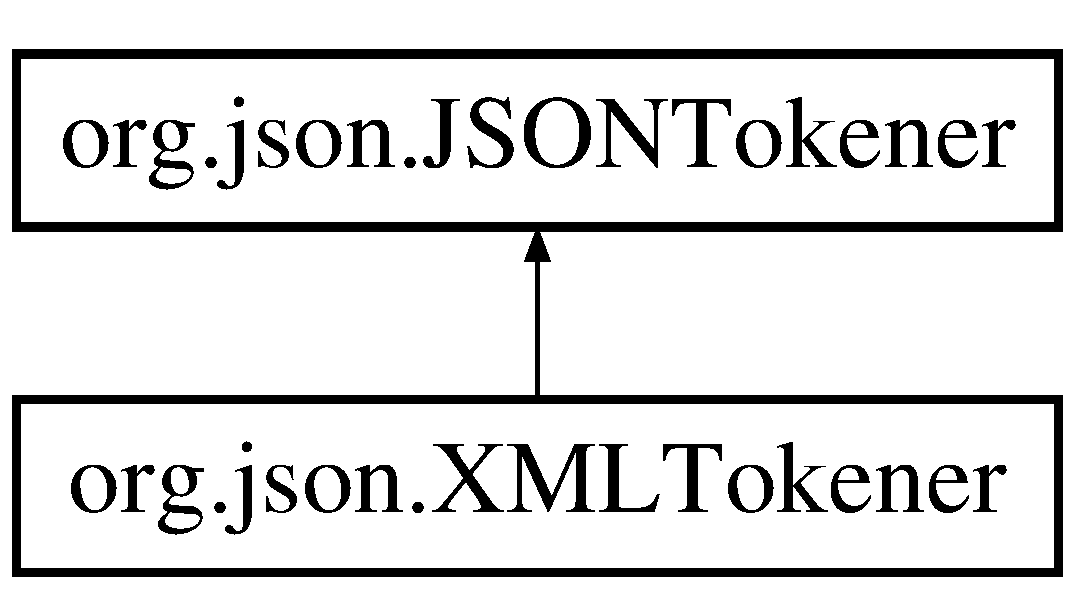
\includegraphics[height=2.000000cm]{classorg_1_1json_1_1_x_m_l_tokener}
\end{center}
\end{figure}
\subsection*{Public Member Functions}
\begin{DoxyCompactItemize}
\item 
\hyperlink{classorg_1_1json_1_1_x_m_l_tokener_a43ba71b6376938f07b4781fb6c66a7ac}{X\-M\-L\-Tokener} (String s)
\item 
String \hyperlink{classorg_1_1json_1_1_x_m_l_tokener_a0f321a2fa10eb19c08d05cf17cfa4e54}{next\-C\-D\-A\-T\-A} ()  throws J\-S\-O\-N\-Exception 
\item 
Object \hyperlink{classorg_1_1json_1_1_x_m_l_tokener_a356e0c4bb50197720b5eb638783b632c}{next\-Content} ()  throws J\-S\-O\-N\-Exception 
\item 
Object \hyperlink{classorg_1_1json_1_1_x_m_l_tokener_aa67ac8eb561a438290fad648fd295fd5}{next\-Entity} (char ampersand)  throws J\-S\-O\-N\-Exception 
\item 
Object \hyperlink{classorg_1_1json_1_1_x_m_l_tokener_aa36d5f6baf25f85fef0468fadcc3b8ff}{next\-Meta} ()  throws J\-S\-O\-N\-Exception 
\item 
Object \hyperlink{classorg_1_1json_1_1_x_m_l_tokener_a654e38e5abe2ad37e10f968613dab875}{next\-Token} ()  throws J\-S\-O\-N\-Exception 
\item 
boolean \hyperlink{classorg_1_1json_1_1_x_m_l_tokener_ac6dd60ff4fa12f0603ac8059f6036810}{skip\-Past} (String to)  throws J\-S\-O\-N\-Exception 
\end{DoxyCompactItemize}
\subsection*{Static Public Attributes}
\begin{DoxyCompactItemize}
\item 
static final java.\-util.\-Hash\-Map \hyperlink{classorg_1_1json_1_1_x_m_l_tokener_ac0e11bf2c9d16e89993773e8510d44b7}{entity}
\end{DoxyCompactItemize}
\subsection*{Static Package Functions}
\begin{DoxyCompactItemize}
\item 
\hyperlink{classorg_1_1json_1_1_x_m_l_tokener_affe5431a4051cdede936b836296cd059}{\mbox{[}static initializer\mbox{]}}
\end{DoxyCompactItemize}
\subsection*{Additional Inherited Members}


\subsection{Detailed Description}
The \hyperlink{classorg_1_1json_1_1_x_m_l_tokener}{X\-M\-L\-Tokener} extends the \hyperlink{classorg_1_1json_1_1_j_s_o_n_tokener}{J\-S\-O\-N\-Tokener} to provide additional methods for the parsing of \hyperlink{classorg_1_1json_1_1_x_m_l}{X\-M\-L} texts. \begin{DoxyAuthor}{Author}
J\-S\-O\-N.\-org 
\end{DoxyAuthor}
\begin{DoxyVersion}{Version}
2012-\/11-\/13 
\end{DoxyVersion}


Definition at line 33 of file X\-M\-L\-Tokener.\-java.



\subsection{Constructor \& Destructor Documentation}
\hypertarget{classorg_1_1json_1_1_x_m_l_tokener_a43ba71b6376938f07b4781fb6c66a7ac}{\index{org\-::json\-::\-X\-M\-L\-Tokener@{org\-::json\-::\-X\-M\-L\-Tokener}!X\-M\-L\-Tokener@{X\-M\-L\-Tokener}}
\index{X\-M\-L\-Tokener@{X\-M\-L\-Tokener}!org::json::XMLTokener@{org\-::json\-::\-X\-M\-L\-Tokener}}
\subsubsection[{X\-M\-L\-Tokener}]{\setlength{\rightskip}{0pt plus 5cm}org.\-json.\-X\-M\-L\-Tokener.\-X\-M\-L\-Tokener (
\begin{DoxyParamCaption}
\item[{String}]{s}
\end{DoxyParamCaption}
)}}\label{classorg_1_1json_1_1_x_m_l_tokener_a43ba71b6376938f07b4781fb6c66a7ac}
Construct an \hyperlink{classorg_1_1json_1_1_x_m_l_tokener}{X\-M\-L\-Tokener} from a string. 
\begin{DoxyParams}{Parameters}
{\em s} & A source string. \\
\hline
\end{DoxyParams}


Definition at line 54 of file X\-M\-L\-Tokener.\-java.


\begin{DoxyCode}
54                                 \{
55         super(s);
56     \}
\end{DoxyCode}


\subsection{Member Function Documentation}
\hypertarget{classorg_1_1json_1_1_x_m_l_tokener_affe5431a4051cdede936b836296cd059}{\index{org\-::json\-::\-X\-M\-L\-Tokener@{org\-::json\-::\-X\-M\-L\-Tokener}!\mbox{[}static initializer\mbox{]}@{[static initializer]}}
\index{\mbox{[}static initializer\mbox{]}@{[static initializer]}!org::json::XMLTokener@{org\-::json\-::\-X\-M\-L\-Tokener}}
\subsubsection[{[static initializer]}]{\setlength{\rightskip}{0pt plus 5cm}org.\-json.\-X\-M\-L\-Tokener.\mbox{[}static initializer\mbox{]} (
\begin{DoxyParamCaption}
{}
\end{DoxyParamCaption}
)\hspace{0.3cm}{\ttfamily [static]}, {\ttfamily [package]}}}\label{classorg_1_1json_1_1_x_m_l_tokener_affe5431a4051cdede936b836296cd059}
\hypertarget{classorg_1_1json_1_1_x_m_l_tokener_a0f321a2fa10eb19c08d05cf17cfa4e54}{\index{org\-::json\-::\-X\-M\-L\-Tokener@{org\-::json\-::\-X\-M\-L\-Tokener}!next\-C\-D\-A\-T\-A@{next\-C\-D\-A\-T\-A}}
\index{next\-C\-D\-A\-T\-A@{next\-C\-D\-A\-T\-A}!org::json::XMLTokener@{org\-::json\-::\-X\-M\-L\-Tokener}}
\subsubsection[{next\-C\-D\-A\-T\-A}]{\setlength{\rightskip}{0pt plus 5cm}String org.\-json.\-X\-M\-L\-Tokener.\-next\-C\-D\-A\-T\-A (
\begin{DoxyParamCaption}
{}
\end{DoxyParamCaption}
) throws {\bf J\-S\-O\-N\-Exception}}}\label{classorg_1_1json_1_1_x_m_l_tokener_a0f321a2fa10eb19c08d05cf17cfa4e54}
Get the text in the C\-D\-A\-T\-A block. \begin{DoxyReturn}{Returns}
The string up to the {\ttfamily \mbox{]}\mbox{]}$>$}. 
\end{DoxyReturn}

\begin{DoxyExceptions}{Exceptions}
{\em \hyperlink{classorg_1_1json_1_1_j_s_o_n_exception}{J\-S\-O\-N\-Exception}} & If the {\ttfamily \mbox{]}\mbox{]}$>$} is not found. \\
\hline
\end{DoxyExceptions}


Definition at line 63 of file X\-M\-L\-Tokener.\-java.



References org.\-json.\-J\-S\-O\-N\-Tokener.\-end(), org.\-json.\-J\-S\-O\-N\-Tokener.\-next(), and org.\-json.\-J\-S\-O\-N\-Tokener.\-syntax\-Error().


\begin{DoxyCode}
63                                                    \{
64         \textcolor{keywordtype}{char}         c;
65         \textcolor{keywordtype}{int}          i;
66         StringBuffer sb = \textcolor{keyword}{new} StringBuffer();
67         \textcolor{keywordflow}{for} (;;) \{
68             c = \hyperlink{classorg_1_1json_1_1_j_s_o_n_tokener_ae129753dbe43ea50aa34e3c06773fdfb}{next}();
69             \textcolor{keywordflow}{if} (\hyperlink{classorg_1_1json_1_1_j_s_o_n_tokener_a767d3f6c8313e03bc3dfb4fdc495294c}{end}()) \{
70                 \textcolor{keywordflow}{throw} \hyperlink{classorg_1_1json_1_1_j_s_o_n_tokener_a467f559950c039f28394ce3a0d2659ca}{syntaxError}(\textcolor{stringliteral}{"Unclosed CDATA"});
71             \}
72             sb.append(c);
73             i = sb.length() - 3;
74             \textcolor{keywordflow}{if} (i >= 0 && sb.charAt(i) == \textcolor{charliteral}{']'} &&
75                           sb.charAt(i + 1) == \textcolor{charliteral}{']'} && sb.charAt(i + 2) == \textcolor{charliteral}{'>'}) \{
76                 sb.setLength(i);
77                 \textcolor{keywordflow}{return} sb.toString();
78             \}
79         \}
80     \}
\end{DoxyCode}
\hypertarget{classorg_1_1json_1_1_x_m_l_tokener_a356e0c4bb50197720b5eb638783b632c}{\index{org\-::json\-::\-X\-M\-L\-Tokener@{org\-::json\-::\-X\-M\-L\-Tokener}!next\-Content@{next\-Content}}
\index{next\-Content@{next\-Content}!org::json::XMLTokener@{org\-::json\-::\-X\-M\-L\-Tokener}}
\subsubsection[{next\-Content}]{\setlength{\rightskip}{0pt plus 5cm}Object org.\-json.\-X\-M\-L\-Tokener.\-next\-Content (
\begin{DoxyParamCaption}
{}
\end{DoxyParamCaption}
) throws {\bf J\-S\-O\-N\-Exception}}}\label{classorg_1_1json_1_1_x_m_l_tokener_a356e0c4bb50197720b5eb638783b632c}
Get the next \hyperlink{classorg_1_1json_1_1_x_m_l}{X\-M\-L} outer token, trimming whitespace. There are two kinds of tokens\-: the '$<$' character which begins a markup tag, and the content text between markup tags.

\begin{DoxyReturn}{Returns}
A string, or a '$<$' Character, or null if there is no more source text. 
\end{DoxyReturn}

\begin{DoxyExceptions}{Exceptions}
{\em \hyperlink{classorg_1_1json_1_1_j_s_o_n_exception}{J\-S\-O\-N\-Exception}} & \\
\hline
\end{DoxyExceptions}


Definition at line 92 of file X\-M\-L\-Tokener.\-java.



References org.\-json.\-J\-S\-O\-N\-Tokener.\-back(), org.\-json.\-X\-M\-L.\-L\-T, org.\-json.\-J\-S\-O\-N\-Tokener.\-next(), and org.\-json.\-X\-M\-L\-Tokener.\-next\-Entity().


\begin{DoxyCode}
92                                                      \{
93         \textcolor{keywordtype}{char}         c;
94         StringBuffer sb;
95         \textcolor{keywordflow}{do} \{
96             c = \hyperlink{classorg_1_1json_1_1_j_s_o_n_tokener_ae129753dbe43ea50aa34e3c06773fdfb}{next}();
97         \} \textcolor{keywordflow}{while} (Character.isWhitespace(c));
98         \textcolor{keywordflow}{if} (c == 0) \{
99             \textcolor{keywordflow}{return} null;
100         \}
101         \textcolor{keywordflow}{if} (c == \textcolor{charliteral}{'<'}) \{
102             \textcolor{keywordflow}{return} XML.LT;
103         \}
104         sb = \textcolor{keyword}{new} StringBuffer();
105         \textcolor{keywordflow}{for} (;;) \{
106             \textcolor{keywordflow}{if} (c == \textcolor{charliteral}{'<'} || c == 0) \{
107                 \hyperlink{classorg_1_1json_1_1_j_s_o_n_tokener_aa2eafdef7304777a457f3e66cc0e668b}{back}();
108                 \textcolor{keywordflow}{return} sb.toString().trim();
109             \}
110             \textcolor{keywordflow}{if} (c == \textcolor{charliteral}{'&'}) \{
111                 sb.append(\hyperlink{classorg_1_1json_1_1_x_m_l_tokener_aa67ac8eb561a438290fad648fd295fd5}{nextEntity}(c));
112             \} \textcolor{keywordflow}{else} \{
113                 sb.append(c);
114             \}
115             c = \hyperlink{classorg_1_1json_1_1_j_s_o_n_tokener_ae129753dbe43ea50aa34e3c06773fdfb}{next}();
116         \}
117     \}
\end{DoxyCode}
\hypertarget{classorg_1_1json_1_1_x_m_l_tokener_aa67ac8eb561a438290fad648fd295fd5}{\index{org\-::json\-::\-X\-M\-L\-Tokener@{org\-::json\-::\-X\-M\-L\-Tokener}!next\-Entity@{next\-Entity}}
\index{next\-Entity@{next\-Entity}!org::json::XMLTokener@{org\-::json\-::\-X\-M\-L\-Tokener}}
\subsubsection[{next\-Entity}]{\setlength{\rightskip}{0pt plus 5cm}Object org.\-json.\-X\-M\-L\-Tokener.\-next\-Entity (
\begin{DoxyParamCaption}
\item[{char}]{ampersand}
\end{DoxyParamCaption}
) throws {\bf J\-S\-O\-N\-Exception}}}\label{classorg_1_1json_1_1_x_m_l_tokener_aa67ac8eb561a438290fad648fd295fd5}
Return the next entity. These entities are translated to Characters\-: {\ttfamily \& ' $>$ $<$ "}. 
\begin{DoxyParams}{Parameters}
{\em ampersand} & An ampersand character. \\
\hline
\end{DoxyParams}
\begin{DoxyReturn}{Returns}
A Character or an entity String if the entity is not recognized. 
\end{DoxyReturn}

\begin{DoxyExceptions}{Exceptions}
{\em \hyperlink{classorg_1_1json_1_1_j_s_o_n_exception}{J\-S\-O\-N\-Exception}} & If missing ';' in \hyperlink{classorg_1_1json_1_1_x_m_l}{X\-M\-L} entity. \\
\hline
\end{DoxyExceptions}


Definition at line 127 of file X\-M\-L\-Tokener.\-java.



References org.\-json.\-X\-M\-L\-Tokener.\-entity, org.\-json.\-J\-S\-O\-N\-Tokener.\-next(), and org.\-json.\-J\-S\-O\-N\-Tokener.\-syntax\-Error().



Referenced by org.\-json.\-X\-M\-L\-Tokener.\-next\-Content(), and org.\-json.\-X\-M\-L\-Tokener.\-next\-Token().


\begin{DoxyCode}
127                                                                   \{
128         StringBuffer sb = \textcolor{keyword}{new} StringBuffer();
129         \textcolor{keywordflow}{for} (;;) \{
130             \textcolor{keywordtype}{char} c = \hyperlink{classorg_1_1json_1_1_j_s_o_n_tokener_ae129753dbe43ea50aa34e3c06773fdfb}{next}();
131             \textcolor{keywordflow}{if} (Character.isLetterOrDigit(c) || c == \textcolor{charliteral}{'#'}) \{
132                 sb.append(Character.toLowerCase(c));
133             \} \textcolor{keywordflow}{else} \textcolor{keywordflow}{if} (c == \textcolor{charliteral}{';'}) \{
134                 \textcolor{keywordflow}{break};
135             \} \textcolor{keywordflow}{else} \{
136                 \textcolor{keywordflow}{throw} \hyperlink{classorg_1_1json_1_1_j_s_o_n_tokener_a467f559950c039f28394ce3a0d2659ca}{syntaxError}(\textcolor{stringliteral}{"Missing ';' in XML entity: &"} + sb);
137             \}
138         \}
139         String \textcolor{keywordtype}{string} = sb.toString();
140         Object \textcolor{keywordtype}{object} = \hyperlink{classorg_1_1json_1_1_x_m_l_tokener_ac0e11bf2c9d16e89993773e8510d44b7}{entity}.get(\textcolor{keywordtype}{string});
141         \textcolor{keywordflow}{return} \textcolor{keywordtype}{object} != null ? \textcolor{keywordtype}{object} : ampersand + \textcolor{keywordtype}{string} + \textcolor{stringliteral}{";"};
142     \}
\end{DoxyCode}
\hypertarget{classorg_1_1json_1_1_x_m_l_tokener_aa36d5f6baf25f85fef0468fadcc3b8ff}{\index{org\-::json\-::\-X\-M\-L\-Tokener@{org\-::json\-::\-X\-M\-L\-Tokener}!next\-Meta@{next\-Meta}}
\index{next\-Meta@{next\-Meta}!org::json::XMLTokener@{org\-::json\-::\-X\-M\-L\-Tokener}}
\subsubsection[{next\-Meta}]{\setlength{\rightskip}{0pt plus 5cm}Object org.\-json.\-X\-M\-L\-Tokener.\-next\-Meta (
\begin{DoxyParamCaption}
{}
\end{DoxyParamCaption}
) throws {\bf J\-S\-O\-N\-Exception}}}\label{classorg_1_1json_1_1_x_m_l_tokener_aa36d5f6baf25f85fef0468fadcc3b8ff}
Returns the next \hyperlink{classorg_1_1json_1_1_x_m_l}{X\-M\-L} meta token. This is used for skipping over $<$!...$>$ and $<$?...?$>$ structures. \begin{DoxyReturn}{Returns}
Syntax characters ({\ttfamily $<$ $>$ / = ! ?}) are returned as Character, and strings and names are returned as Boolean. We don't care what the values actually are. 
\end{DoxyReturn}

\begin{DoxyExceptions}{Exceptions}
{\em \hyperlink{classorg_1_1json_1_1_j_s_o_n_exception}{J\-S\-O\-N\-Exception}} & If a string is not properly closed or if the \hyperlink{classorg_1_1json_1_1_x_m_l}{X\-M\-L} is badly structured. \\
\hline
\end{DoxyExceptions}


Definition at line 154 of file X\-M\-L\-Tokener.\-java.



References org.\-json.\-J\-S\-O\-N\-Tokener.\-back(), org.\-json.\-X\-M\-L.\-B\-A\-N\-G, org.\-json.\-X\-M\-L.\-E\-Q, org.\-json.\-X\-M\-L.\-G\-T, org.\-json.\-X\-M\-L.\-L\-T, org.\-json.\-J\-S\-O\-N\-Tokener.\-next(), org.\-json.\-X\-M\-L.\-Q\-U\-E\-S\-T, org.\-json.\-X\-M\-L.\-S\-L\-A\-S\-H, and org.\-json.\-J\-S\-O\-N\-Tokener.\-syntax\-Error().


\begin{DoxyCode}
154                                                   \{
155         \textcolor{keywordtype}{char} c;
156         \textcolor{keywordtype}{char} q;
157         \textcolor{keywordflow}{do} \{
158             c = \hyperlink{classorg_1_1json_1_1_j_s_o_n_tokener_ae129753dbe43ea50aa34e3c06773fdfb}{next}();
159         \} \textcolor{keywordflow}{while} (Character.isWhitespace(c));
160         \textcolor{keywordflow}{switch} (c) \{
161         \textcolor{keywordflow}{case} 0:
162             \textcolor{keywordflow}{throw} \hyperlink{classorg_1_1json_1_1_j_s_o_n_tokener_a467f559950c039f28394ce3a0d2659ca}{syntaxError}(\textcolor{stringliteral}{"Misshaped meta tag"});
163         \textcolor{keywordflow}{case} \textcolor{charliteral}{'<'}:
164             \textcolor{keywordflow}{return} XML.LT;
165         \textcolor{keywordflow}{case} \textcolor{charliteral}{'>'}:
166             \textcolor{keywordflow}{return} XML.GT;
167         \textcolor{keywordflow}{case} \textcolor{charliteral}{'/'}:
168             \textcolor{keywordflow}{return} XML.SLASH;
169         \textcolor{keywordflow}{case} \textcolor{charliteral}{'='}:
170             \textcolor{keywordflow}{return} XML.EQ;
171         \textcolor{keywordflow}{case} \textcolor{charliteral}{'!'}:
172             \textcolor{keywordflow}{return} XML.BANG;
173         \textcolor{keywordflow}{case} \textcolor{charliteral}{'?'}:
174             \textcolor{keywordflow}{return} XML.QUEST;
175         \textcolor{keywordflow}{case} \textcolor{charliteral}{'"'}:
176         \textcolor{keywordflow}{case} \textcolor{charliteral}{'\(\backslash\)''}:
177             q = c;
178             \textcolor{keywordflow}{for} (;;) \{
179                 c = \hyperlink{classorg_1_1json_1_1_j_s_o_n_tokener_ae129753dbe43ea50aa34e3c06773fdfb}{next}();
180                 \textcolor{keywordflow}{if} (c == 0) \{
181                     \textcolor{keywordflow}{throw} \hyperlink{classorg_1_1json_1_1_j_s_o_n_tokener_a467f559950c039f28394ce3a0d2659ca}{syntaxError}(\textcolor{stringliteral}{"Unterminated string"});
182                 \}
183                 \textcolor{keywordflow}{if} (c == q) \{
184                     \textcolor{keywordflow}{return} Boolean.TRUE;
185                 \}
186             \}
187         \textcolor{keywordflow}{default}:
188             \textcolor{keywordflow}{for} (;;) \{
189                 c = \hyperlink{classorg_1_1json_1_1_j_s_o_n_tokener_ae129753dbe43ea50aa34e3c06773fdfb}{next}();
190                 \textcolor{keywordflow}{if} (Character.isWhitespace(c)) \{
191                     \textcolor{keywordflow}{return} Boolean.TRUE;
192                 \}
193                 \textcolor{keywordflow}{switch} (c) \{
194                 \textcolor{keywordflow}{case} 0:
195                 \textcolor{keywordflow}{case} \textcolor{charliteral}{'<'}:
196                 \textcolor{keywordflow}{case} \textcolor{charliteral}{'>'}:
197                 \textcolor{keywordflow}{case} \textcolor{charliteral}{'/'}:
198                 \textcolor{keywordflow}{case} \textcolor{charliteral}{'='}:
199                 \textcolor{keywordflow}{case} \textcolor{charliteral}{'!'}:
200                 \textcolor{keywordflow}{case} \textcolor{charliteral}{'?'}:
201                 \textcolor{keywordflow}{case} \textcolor{charliteral}{'"'}:
202                 \textcolor{keywordflow}{case} \textcolor{charliteral}{'\(\backslash\)''}:
203                     \hyperlink{classorg_1_1json_1_1_j_s_o_n_tokener_aa2eafdef7304777a457f3e66cc0e668b}{back}();
204                     \textcolor{keywordflow}{return} Boolean.TRUE;
205                 \}
206             \}
207         \}
208     \}
\end{DoxyCode}
\hypertarget{classorg_1_1json_1_1_x_m_l_tokener_a654e38e5abe2ad37e10f968613dab875}{\index{org\-::json\-::\-X\-M\-L\-Tokener@{org\-::json\-::\-X\-M\-L\-Tokener}!next\-Token@{next\-Token}}
\index{next\-Token@{next\-Token}!org::json::XMLTokener@{org\-::json\-::\-X\-M\-L\-Tokener}}
\subsubsection[{next\-Token}]{\setlength{\rightskip}{0pt plus 5cm}Object org.\-json.\-X\-M\-L\-Tokener.\-next\-Token (
\begin{DoxyParamCaption}
{}
\end{DoxyParamCaption}
) throws {\bf J\-S\-O\-N\-Exception}}}\label{classorg_1_1json_1_1_x_m_l_tokener_a654e38e5abe2ad37e10f968613dab875}
Get the next \hyperlink{classorg_1_1json_1_1_x_m_l}{X\-M\-L} Token. These tokens are found inside of angle brackets. It may be one of these characters\-: {\ttfamily / $>$ = ! ?} or it may be a string wrapped in single quotes or double quotes, or it may be a name. \begin{DoxyReturn}{Returns}
a String or a Character. 
\end{DoxyReturn}

\begin{DoxyExceptions}{Exceptions}
{\em \hyperlink{classorg_1_1json_1_1_j_s_o_n_exception}{J\-S\-O\-N\-Exception}} & If the \hyperlink{classorg_1_1json_1_1_x_m_l}{X\-M\-L} is not well formed. \\
\hline
\end{DoxyExceptions}


Definition at line 219 of file X\-M\-L\-Tokener.\-java.



References org.\-json.\-J\-S\-O\-N\-Tokener.\-back(), org.\-json.\-X\-M\-L.\-B\-A\-N\-G, org.\-json.\-X\-M\-L.\-E\-Q, org.\-json.\-X\-M\-L.\-G\-T, org.\-json.\-J\-S\-O\-N\-Tokener.\-next(), org.\-json.\-X\-M\-L\-Tokener.\-next\-Entity(), org.\-json.\-X\-M\-L.\-Q\-U\-E\-S\-T, org.\-json.\-X\-M\-L.\-S\-L\-A\-S\-H, and org.\-json.\-J\-S\-O\-N\-Tokener.\-syntax\-Error().


\begin{DoxyCode}
219                                                    \{
220         \textcolor{keywordtype}{char} c;
221         \textcolor{keywordtype}{char} q;
222         StringBuffer sb;
223         \textcolor{keywordflow}{do} \{
224             c = \hyperlink{classorg_1_1json_1_1_j_s_o_n_tokener_ae129753dbe43ea50aa34e3c06773fdfb}{next}();
225         \} \textcolor{keywordflow}{while} (Character.isWhitespace(c));
226         \textcolor{keywordflow}{switch} (c) \{
227         \textcolor{keywordflow}{case} 0:
228             \textcolor{keywordflow}{throw} \hyperlink{classorg_1_1json_1_1_j_s_o_n_tokener_a467f559950c039f28394ce3a0d2659ca}{syntaxError}(\textcolor{stringliteral}{"Misshaped element"});
229         \textcolor{keywordflow}{case} \textcolor{charliteral}{'<'}:
230             \textcolor{keywordflow}{throw} \hyperlink{classorg_1_1json_1_1_j_s_o_n_tokener_a467f559950c039f28394ce3a0d2659ca}{syntaxError}(\textcolor{stringliteral}{"Misplaced '<'"});
231         \textcolor{keywordflow}{case} \textcolor{charliteral}{'>'}:
232             \textcolor{keywordflow}{return} XML.GT;
233         \textcolor{keywordflow}{case} \textcolor{charliteral}{'/'}:
234             \textcolor{keywordflow}{return} XML.SLASH;
235         \textcolor{keywordflow}{case} \textcolor{charliteral}{'='}:
236             \textcolor{keywordflow}{return} XML.EQ;
237         \textcolor{keywordflow}{case} \textcolor{charliteral}{'!'}:
238             \textcolor{keywordflow}{return} XML.BANG;
239         \textcolor{keywordflow}{case} \textcolor{charliteral}{'?'}:
240             \textcolor{keywordflow}{return} XML.QUEST;
241 
242 \textcolor{comment}{// Quoted string}
243 
244         \textcolor{keywordflow}{case} \textcolor{charliteral}{'"'}:
245         \textcolor{keywordflow}{case} \textcolor{charliteral}{'\(\backslash\)''}:
246             q = c;
247             sb = \textcolor{keyword}{new} StringBuffer();
248             \textcolor{keywordflow}{for} (;;) \{
249                 c = \hyperlink{classorg_1_1json_1_1_j_s_o_n_tokener_ae129753dbe43ea50aa34e3c06773fdfb}{next}();
250                 \textcolor{keywordflow}{if} (c == 0) \{
251                     \textcolor{keywordflow}{throw} \hyperlink{classorg_1_1json_1_1_j_s_o_n_tokener_a467f559950c039f28394ce3a0d2659ca}{syntaxError}(\textcolor{stringliteral}{"Unterminated string"});
252                 \}
253                 \textcolor{keywordflow}{if} (c == q) \{
254                     \textcolor{keywordflow}{return} sb.toString();
255                 \}
256                 \textcolor{keywordflow}{if} (c == \textcolor{charliteral}{'&'}) \{
257                     sb.append(\hyperlink{classorg_1_1json_1_1_x_m_l_tokener_aa67ac8eb561a438290fad648fd295fd5}{nextEntity}(c));
258                 \} \textcolor{keywordflow}{else} \{
259                     sb.append(c);
260                 \}
261             \}
262         \textcolor{keywordflow}{default}:
263 
264 \textcolor{comment}{// Name}
265 
266             sb = \textcolor{keyword}{new} StringBuffer();
267             \textcolor{keywordflow}{for} (;;) \{
268                 sb.append(c);
269                 c = \hyperlink{classorg_1_1json_1_1_j_s_o_n_tokener_ae129753dbe43ea50aa34e3c06773fdfb}{next}();
270                 \textcolor{keywordflow}{if} (Character.isWhitespace(c)) \{
271                     \textcolor{keywordflow}{return} sb.toString();
272                 \}
273                 \textcolor{keywordflow}{switch} (c) \{
274                 \textcolor{keywordflow}{case} 0:
275                     \textcolor{keywordflow}{return} sb.toString();
276                 \textcolor{keywordflow}{case} \textcolor{charliteral}{'>'}:
277                 \textcolor{keywordflow}{case} \textcolor{charliteral}{'/'}:
278                 \textcolor{keywordflow}{case} \textcolor{charliteral}{'='}:
279                 \textcolor{keywordflow}{case} \textcolor{charliteral}{'!'}:
280                 \textcolor{keywordflow}{case} \textcolor{charliteral}{'?'}:
281                 \textcolor{keywordflow}{case} \textcolor{charliteral}{'['}:
282                 \textcolor{keywordflow}{case} \textcolor{charliteral}{']'}:
283                     \hyperlink{classorg_1_1json_1_1_j_s_o_n_tokener_aa2eafdef7304777a457f3e66cc0e668b}{back}();
284                     \textcolor{keywordflow}{return} sb.toString();
285                 \textcolor{keywordflow}{case} \textcolor{charliteral}{'<'}:
286                 \textcolor{keywordflow}{case} \textcolor{charliteral}{'"'}:
287                 \textcolor{keywordflow}{case} \textcolor{charliteral}{'\(\backslash\)''}:
288                     \textcolor{keywordflow}{throw} \hyperlink{classorg_1_1json_1_1_j_s_o_n_tokener_a467f559950c039f28394ce3a0d2659ca}{syntaxError}(\textcolor{stringliteral}{"Bad character in a name"});
289                 \}
290             \}
291         \}
292     \}
\end{DoxyCode}
\hypertarget{classorg_1_1json_1_1_x_m_l_tokener_ac6dd60ff4fa12f0603ac8059f6036810}{\index{org\-::json\-::\-X\-M\-L\-Tokener@{org\-::json\-::\-X\-M\-L\-Tokener}!skip\-Past@{skip\-Past}}
\index{skip\-Past@{skip\-Past}!org::json::XMLTokener@{org\-::json\-::\-X\-M\-L\-Tokener}}
\subsubsection[{skip\-Past}]{\setlength{\rightskip}{0pt plus 5cm}boolean org.\-json.\-X\-M\-L\-Tokener.\-skip\-Past (
\begin{DoxyParamCaption}
\item[{String}]{to}
\end{DoxyParamCaption}
) throws {\bf J\-S\-O\-N\-Exception}}}\label{classorg_1_1json_1_1_x_m_l_tokener_ac6dd60ff4fa12f0603ac8059f6036810}
Skip characters until past the requested string. If it is not found, we are left at the end of the source with a result of false. 
\begin{DoxyParams}{Parameters}
{\em to} & A string to skip past. \\
\hline
\end{DoxyParams}

\begin{DoxyExceptions}{Exceptions}
{\em \hyperlink{classorg_1_1json_1_1_j_s_o_n_exception}{J\-S\-O\-N\-Exception}} & \\
\hline
\end{DoxyExceptions}


Definition at line 301 of file X\-M\-L\-Tokener.\-java.



References org.\-json.\-J\-S\-O\-N\-Tokener.\-next().



Referenced by org.\-json.\-X\-M\-L.\-to\-J\-S\-O\-N\-Object().


\begin{DoxyCode}
301                                                             \{
302         \textcolor{keywordtype}{boolean} b;
303         \textcolor{keywordtype}{char} c;
304         \textcolor{keywordtype}{int} i;
305         \textcolor{keywordtype}{int} j;
306         \textcolor{keywordtype}{int} offset = 0;
307         \textcolor{keywordtype}{int} length = to.length();
308         \textcolor{keywordtype}{char}[] circle = \textcolor{keyword}{new} \textcolor{keywordtype}{char}[length];
309 
310         \textcolor{comment}{/*}
311 \textcolor{comment}{         * First fill the circle buffer with as many characters as are in the}
312 \textcolor{comment}{         * to string. If we reach an early end, bail.}
313 \textcolor{comment}{         */}
314 
315         \textcolor{keywordflow}{for} (i = 0; i < length; i += 1) \{
316             c = \hyperlink{classorg_1_1json_1_1_j_s_o_n_tokener_ae129753dbe43ea50aa34e3c06773fdfb}{next}();
317             \textcolor{keywordflow}{if} (c == 0) \{
318                 \textcolor{keywordflow}{return} \textcolor{keyword}{false};
319             \}
320             circle[i] = c;
321         \}
322 
323         \textcolor{comment}{/* We will loop, possibly for all of the remaining characters. */}
324 
325         \textcolor{keywordflow}{for} (;;) \{
326             j = offset;
327             b = \textcolor{keyword}{true};
328 
329             \textcolor{comment}{/* Compare the circle buffer with the to string. */}
330 
331             \textcolor{keywordflow}{for} (i = 0; i < length; i += 1) \{
332                 \textcolor{keywordflow}{if} (circle[j] != to.charAt(i)) \{
333                     b = \textcolor{keyword}{false};
334                     \textcolor{keywordflow}{break};
335                 \}
336                 j += 1;
337                 \textcolor{keywordflow}{if} (j >= length) \{
338                     j -= length;
339                 \}
340             \}
341 
342             \textcolor{comment}{/* If we exit the loop with b intact, then victory is ours. */}
343 
344             \textcolor{keywordflow}{if} (b) \{
345                 \textcolor{keywordflow}{return} \textcolor{keyword}{true};
346             \}
347 
348             \textcolor{comment}{/* Get the next character. If there isn't one, then defeat is ours. */}
349 
350             c = \hyperlink{classorg_1_1json_1_1_j_s_o_n_tokener_ae129753dbe43ea50aa34e3c06773fdfb}{next}();
351             \textcolor{keywordflow}{if} (c == 0) \{
352                 \textcolor{keywordflow}{return} \textcolor{keyword}{false};
353             \}
354             \textcolor{comment}{/*}
355 \textcolor{comment}{             * Shove the character in the circle buffer and advance the}
356 \textcolor{comment}{             * circle offset. The offset is mod n.}
357 \textcolor{comment}{             */}
358             circle[offset] = c;
359             offset += 1;
360             \textcolor{keywordflow}{if} (offset >= length) \{
361                 offset -= length;
362             \}
363         \}
364     \}
\end{DoxyCode}


\subsection{Member Data Documentation}
\hypertarget{classorg_1_1json_1_1_x_m_l_tokener_ac0e11bf2c9d16e89993773e8510d44b7}{\index{org\-::json\-::\-X\-M\-L\-Tokener@{org\-::json\-::\-X\-M\-L\-Tokener}!entity@{entity}}
\index{entity@{entity}!org::json::XMLTokener@{org\-::json\-::\-X\-M\-L\-Tokener}}
\subsubsection[{entity}]{\setlength{\rightskip}{0pt plus 5cm}final java.\-util.\-Hash\-Map org.\-json.\-X\-M\-L\-Tokener.\-entity\hspace{0.3cm}{\ttfamily [static]}}}\label{classorg_1_1json_1_1_x_m_l_tokener_ac0e11bf2c9d16e89993773e8510d44b7}
The table of entity values. It initially contains Character values for amp, apos, gt, lt, quot. 

Definition at line 39 of file X\-M\-L\-Tokener.\-java.



Referenced by org.\-json.\-X\-M\-L\-Tokener.\-next\-Entity().



The documentation for this class was generated from the following file\-:\begin{DoxyCompactItemize}
\item 
org/json/\hyperlink{_x_m_l_tokener_8java}{X\-M\-L\-Tokener.\-java}\end{DoxyCompactItemize}

\chapter{File Documentation}
\hypertarget{dbinsert_8java}{\section{dbinsert.\-java File Reference}
\label{dbinsert_8java}\index{dbinsert.\-java@{dbinsert.\-java}}
}
\subsection*{Classes}
\begin{DoxyCompactItemize}
\item 
class \hyperlink{classdbinsert}{dbinsert}
\end{DoxyCompactItemize}

\hypertarget{_crawler_client_8java}{\section{org/facebook/crawler/\-Crawler\-Client.java File Reference}
\label{_crawler_client_8java}\index{org/facebook/crawler/\-Crawler\-Client.\-java@{org/facebook/crawler/\-Crawler\-Client.\-java}}
}
\subsection*{Classes}
\begin{DoxyCompactItemize}
\item 
class \hyperlink{classorg_1_1facebook_1_1crawler_1_1_crawler_client}{org.\-facebook.\-crawler.\-Crawler\-Client}
\end{DoxyCompactItemize}
\subsection*{Packages}
\begin{DoxyCompactItemize}
\item 
package \hyperlink{namespaceorg_1_1facebook_1_1crawler}{org.\-facebook.\-crawler}
\end{DoxyCompactItemize}

\hypertarget{_facebook_database_8java}{\section{org/facebook/crawler/\-Facebook\-Database.java File Reference}
\label{_facebook_database_8java}\index{org/facebook/crawler/\-Facebook\-Database.\-java@{org/facebook/crawler/\-Facebook\-Database.\-java}}
}
\subsection*{Classes}
\begin{DoxyCompactItemize}
\item 
class \hyperlink{classorg_1_1facebook_1_1crawler_1_1_facebook_database}{org.\-facebook.\-crawler.\-Facebook\-Database}
\end{DoxyCompactItemize}
\subsection*{Packages}
\begin{DoxyCompactItemize}
\item 
package \hyperlink{namespaceorg_1_1facebook_1_1crawler}{org.\-facebook.\-crawler}
\end{DoxyCompactItemize}

\hypertarget{_facebook_d_b_params_8java}{\section{org/facebook/crawler/\-Facebook\-D\-B\-Params.java File Reference}
\label{_facebook_d_b_params_8java}\index{org/facebook/crawler/\-Facebook\-D\-B\-Params.\-java@{org/facebook/crawler/\-Facebook\-D\-B\-Params.\-java}}
}
\subsection*{Classes}
\begin{DoxyCompactItemize}
\item 
class \hyperlink{classorg_1_1facebook_1_1crawler_1_1_facebook_d_b_params}{org.\-facebook.\-crawler.\-Facebook\-D\-B\-Params}
\end{DoxyCompactItemize}
\subsection*{Packages}
\begin{DoxyCompactItemize}
\item 
package \hyperlink{namespaceorg_1_1facebook_1_1crawler}{org.\-facebook.\-crawler}
\end{DoxyCompactItemize}

\hypertarget{_facebook_json_parser_8java}{\section{org/facebook/crawler/\-Facebook\-Json\-Parser.java File Reference}
\label{_facebook_json_parser_8java}\index{org/facebook/crawler/\-Facebook\-Json\-Parser.\-java@{org/facebook/crawler/\-Facebook\-Json\-Parser.\-java}}
}
\subsection*{Classes}
\begin{DoxyCompactItemize}
\item 
enum \hyperlink{enumorg_1_1facebook_1_1crawler_1_1_crawl_options}{org.\-facebook.\-crawler.\-Crawl\-Options}
\item 
class \hyperlink{classorg_1_1facebook_1_1crawler_1_1_facebook_json_parser}{org.\-facebook.\-crawler.\-Facebook\-Json\-Parser}
\end{DoxyCompactItemize}
\subsection*{Packages}
\begin{DoxyCompactItemize}
\item 
package \hyperlink{namespaceorg_1_1facebook_1_1crawler}{org.\-facebook.\-crawler}
\end{DoxyCompactItemize}

\hypertarget{_c_d_l_8java}{\section{org/json/\-C\-D\-L.java File Reference}
\label{_c_d_l_8java}\index{org/json/\-C\-D\-L.\-java@{org/json/\-C\-D\-L.\-java}}
}
\subsection*{Classes}
\begin{DoxyCompactItemize}
\item 
class \hyperlink{classorg_1_1json_1_1_c_d_l}{org.\-json.\-C\-D\-L}
\end{DoxyCompactItemize}
\subsection*{Packages}
\begin{DoxyCompactItemize}
\item 
package \hyperlink{namespaceorg_1_1json}{org.\-json}
\end{DoxyCompactItemize}

\hypertarget{_cookie_8java}{\section{org/json/\-Cookie.java File Reference}
\label{_cookie_8java}\index{org/json/\-Cookie.\-java@{org/json/\-Cookie.\-java}}
}
\subsection*{Classes}
\begin{DoxyCompactItemize}
\item 
class \hyperlink{classorg_1_1json_1_1_cookie}{org.\-json.\-Cookie}
\end{DoxyCompactItemize}
\subsection*{Packages}
\begin{DoxyCompactItemize}
\item 
package \hyperlink{namespaceorg_1_1json}{org.\-json}
\end{DoxyCompactItemize}

\hypertarget{_cookie_list_8java}{\section{org/json/\-Cookie\-List.java File Reference}
\label{_cookie_list_8java}\index{org/json/\-Cookie\-List.\-java@{org/json/\-Cookie\-List.\-java}}
}
\subsection*{Classes}
\begin{DoxyCompactItemize}
\item 
class \hyperlink{classorg_1_1json_1_1_cookie_list}{org.\-json.\-Cookie\-List}
\end{DoxyCompactItemize}
\subsection*{Packages}
\begin{DoxyCompactItemize}
\item 
package \hyperlink{namespaceorg_1_1json}{org.\-json}
\end{DoxyCompactItemize}

\hypertarget{_h_t_t_p_8java}{\section{org/json/\-H\-T\-T\-P.java File Reference}
\label{_h_t_t_p_8java}\index{org/json/\-H\-T\-T\-P.\-java@{org/json/\-H\-T\-T\-P.\-java}}
}
\subsection*{Classes}
\begin{DoxyCompactItemize}
\item 
class \hyperlink{classorg_1_1json_1_1_h_t_t_p}{org.\-json.\-H\-T\-T\-P}
\end{DoxyCompactItemize}
\subsection*{Packages}
\begin{DoxyCompactItemize}
\item 
package \hyperlink{namespaceorg_1_1json}{org.\-json}
\end{DoxyCompactItemize}

\hypertarget{_h_t_t_p_tokener_8java}{\section{org/json/\-H\-T\-T\-P\-Tokener.java File Reference}
\label{_h_t_t_p_tokener_8java}\index{org/json/\-H\-T\-T\-P\-Tokener.\-java@{org/json/\-H\-T\-T\-P\-Tokener.\-java}}
}
\subsection*{Classes}
\begin{DoxyCompactItemize}
\item 
class \hyperlink{classorg_1_1json_1_1_h_t_t_p_tokener}{org.\-json.\-H\-T\-T\-P\-Tokener}
\end{DoxyCompactItemize}
\subsection*{Packages}
\begin{DoxyCompactItemize}
\item 
package \hyperlink{namespaceorg_1_1json}{org.\-json}
\end{DoxyCompactItemize}

\hypertarget{_j_s_o_n_array_8java}{\section{org/json/\-J\-S\-O\-N\-Array.java File Reference}
\label{_j_s_o_n_array_8java}\index{org/json/\-J\-S\-O\-N\-Array.\-java@{org/json/\-J\-S\-O\-N\-Array.\-java}}
}
\subsection*{Classes}
\begin{DoxyCompactItemize}
\item 
class \hyperlink{classorg_1_1json_1_1_j_s_o_n_array}{org.\-json.\-J\-S\-O\-N\-Array}
\end{DoxyCompactItemize}
\subsection*{Packages}
\begin{DoxyCompactItemize}
\item 
package \hyperlink{namespaceorg_1_1json}{org.\-json}
\end{DoxyCompactItemize}

\hypertarget{_j_s_o_n_exception_8java}{\section{org/json/\-J\-S\-O\-N\-Exception.java File Reference}
\label{_j_s_o_n_exception_8java}\index{org/json/\-J\-S\-O\-N\-Exception.\-java@{org/json/\-J\-S\-O\-N\-Exception.\-java}}
}
\subsection*{Classes}
\begin{DoxyCompactItemize}
\item 
class \hyperlink{classorg_1_1json_1_1_j_s_o_n_exception}{org.\-json.\-J\-S\-O\-N\-Exception}
\end{DoxyCompactItemize}
\subsection*{Packages}
\begin{DoxyCompactItemize}
\item 
package \hyperlink{namespaceorg_1_1json}{org.\-json}
\end{DoxyCompactItemize}

\hypertarget{_j_s_o_n_m_l_8java}{\section{org/json/\-J\-S\-O\-N\-M\-L.java File Reference}
\label{_j_s_o_n_m_l_8java}\index{org/json/\-J\-S\-O\-N\-M\-L.\-java@{org/json/\-J\-S\-O\-N\-M\-L.\-java}}
}
\subsection*{Classes}
\begin{DoxyCompactItemize}
\item 
class \hyperlink{classorg_1_1json_1_1_j_s_o_n_m_l}{org.\-json.\-J\-S\-O\-N\-M\-L}
\end{DoxyCompactItemize}
\subsection*{Packages}
\begin{DoxyCompactItemize}
\item 
package \hyperlink{namespaceorg_1_1json}{org.\-json}
\end{DoxyCompactItemize}

\hypertarget{_j_s_o_n_object_8java}{\section{org/json/\-J\-S\-O\-N\-Object.java File Reference}
\label{_j_s_o_n_object_8java}\index{org/json/\-J\-S\-O\-N\-Object.\-java@{org/json/\-J\-S\-O\-N\-Object.\-java}}
}
\subsection*{Classes}
\begin{DoxyCompactItemize}
\item 
class \hyperlink{classorg_1_1json_1_1_j_s_o_n_object}{org.\-json.\-J\-S\-O\-N\-Object}
\item 
class \hyperlink{classorg_1_1json_1_1_j_s_o_n_object_1_1_null}{org.\-json.\-J\-S\-O\-N\-Object.\-Null}
\end{DoxyCompactItemize}
\subsection*{Packages}
\begin{DoxyCompactItemize}
\item 
package \hyperlink{namespaceorg_1_1json}{org.\-json}
\end{DoxyCompactItemize}

\hypertarget{_j_s_o_n_string_8java}{\section{org/json/\-J\-S\-O\-N\-String.java File Reference}
\label{_j_s_o_n_string_8java}\index{org/json/\-J\-S\-O\-N\-String.\-java@{org/json/\-J\-S\-O\-N\-String.\-java}}
}
\subsection*{Classes}
\begin{DoxyCompactItemize}
\item 
interface \hyperlink{interfaceorg_1_1json_1_1_j_s_o_n_string}{org.\-json.\-J\-S\-O\-N\-String}
\end{DoxyCompactItemize}
\subsection*{Packages}
\begin{DoxyCompactItemize}
\item 
package \hyperlink{namespaceorg_1_1json}{org.\-json}
\end{DoxyCompactItemize}

\hypertarget{_j_s_o_n_stringer_8java}{\section{org/json/\-J\-S\-O\-N\-Stringer.java File Reference}
\label{_j_s_o_n_stringer_8java}\index{org/json/\-J\-S\-O\-N\-Stringer.\-java@{org/json/\-J\-S\-O\-N\-Stringer.\-java}}
}
\subsection*{Classes}
\begin{DoxyCompactItemize}
\item 
class \hyperlink{classorg_1_1json_1_1_j_s_o_n_stringer}{org.\-json.\-J\-S\-O\-N\-Stringer}
\end{DoxyCompactItemize}
\subsection*{Packages}
\begin{DoxyCompactItemize}
\item 
package \hyperlink{namespaceorg_1_1json}{org.\-json}
\end{DoxyCompactItemize}

\hypertarget{_j_s_o_n_tokener_8java}{\section{org/json/\-J\-S\-O\-N\-Tokener.java File Reference}
\label{_j_s_o_n_tokener_8java}\index{org/json/\-J\-S\-O\-N\-Tokener.\-java@{org/json/\-J\-S\-O\-N\-Tokener.\-java}}
}
\subsection*{Classes}
\begin{DoxyCompactItemize}
\item 
class \hyperlink{classorg_1_1json_1_1_j_s_o_n_tokener}{org.\-json.\-J\-S\-O\-N\-Tokener}
\end{DoxyCompactItemize}
\subsection*{Packages}
\begin{DoxyCompactItemize}
\item 
package \hyperlink{namespaceorg_1_1json}{org.\-json}
\end{DoxyCompactItemize}

\hypertarget{_j_s_o_n_writer_8java}{\section{org/json/\-J\-S\-O\-N\-Writer.java File Reference}
\label{_j_s_o_n_writer_8java}\index{org/json/\-J\-S\-O\-N\-Writer.\-java@{org/json/\-J\-S\-O\-N\-Writer.\-java}}
}
\subsection*{Classes}
\begin{DoxyCompactItemize}
\item 
class \hyperlink{classorg_1_1json_1_1_j_s_o_n_writer}{org.\-json.\-J\-S\-O\-N\-Writer}
\end{DoxyCompactItemize}
\subsection*{Packages}
\begin{DoxyCompactItemize}
\item 
package \hyperlink{namespaceorg_1_1json}{org.\-json}
\end{DoxyCompactItemize}

\hypertarget{_kim_8java}{\section{org/json/\-Kim.java File Reference}
\label{_kim_8java}\index{org/json/\-Kim.\-java@{org/json/\-Kim.\-java}}
}
\subsection*{Classes}
\begin{DoxyCompactItemize}
\item 
class \hyperlink{classorg_1_1json_1_1_kim}{org.\-json.\-Kim}
\end{DoxyCompactItemize}
\subsection*{Packages}
\begin{DoxyCompactItemize}
\item 
package \hyperlink{namespaceorg_1_1json}{org.\-json}
\end{DoxyCompactItemize}

\hypertarget{_property_8java}{\section{org/json/\-Property.java File Reference}
\label{_property_8java}\index{org/json/\-Property.\-java@{org/json/\-Property.\-java}}
}
\subsection*{Classes}
\begin{DoxyCompactItemize}
\item 
class \hyperlink{classorg_1_1json_1_1_property}{org.\-json.\-Property}
\end{DoxyCompactItemize}
\subsection*{Packages}
\begin{DoxyCompactItemize}
\item 
package \hyperlink{namespaceorg_1_1json}{org.\-json}
\end{DoxyCompactItemize}

\hypertarget{_x_m_l_8java}{\section{org/json/\-X\-M\-L.java File Reference}
\label{_x_m_l_8java}\index{org/json/\-X\-M\-L.\-java@{org/json/\-X\-M\-L.\-java}}
}
\subsection*{Classes}
\begin{DoxyCompactItemize}
\item 
class \hyperlink{classorg_1_1json_1_1_x_m_l}{org.\-json.\-X\-M\-L}
\end{DoxyCompactItemize}
\subsection*{Packages}
\begin{DoxyCompactItemize}
\item 
package \hyperlink{namespaceorg_1_1json}{org.\-json}
\end{DoxyCompactItemize}

\hypertarget{_x_m_l_tokener_8java}{\section{org/json/\-X\-M\-L\-Tokener.java File Reference}
\label{_x_m_l_tokener_8java}\index{org/json/\-X\-M\-L\-Tokener.\-java@{org/json/\-X\-M\-L\-Tokener.\-java}}
}
\subsection*{Classes}
\begin{DoxyCompactItemize}
\item 
class \hyperlink{classorg_1_1json_1_1_x_m_l_tokener}{org.\-json.\-X\-M\-L\-Tokener}
\end{DoxyCompactItemize}
\subsection*{Packages}
\begin{DoxyCompactItemize}
\item 
package \hyperlink{namespaceorg_1_1json}{org.\-json}
\end{DoxyCompactItemize}

\hypertarget{scraperjson_8java}{\section{scraperjson.\-java File Reference}
\label{scraperjson_8java}\index{scraperjson.\-java@{scraperjson.\-java}}
}
\subsection*{Classes}
\begin{DoxyCompactItemize}
\item 
class \hyperlink{class_json_reader}{Json\-Reader}
\end{DoxyCompactItemize}

\hypertarget{scraping_8java}{\section{scraping.\-java File Reference}
\label{scraping_8java}\index{scraping.\-java@{scraping.\-java}}
}
\subsection*{Classes}
\begin{DoxyCompactItemize}
\item 
class \hyperlink{class_facebook_deep_crawl}{Facebook\-Deep\-Crawl}
\end{DoxyCompactItemize}

\hypertarget{voterscraper_8java}{\section{voterscraper.\-java File Reference}
\label{voterscraper_8java}\index{voterscraper.\-java@{voterscraper.\-java}}
}
\subsection*{Classes}
\begin{DoxyCompactItemize}
\item 
class \hyperlink{classvoterscraper}{voterscraper}
\end{DoxyCompactItemize}

%--- End generated contents ---

% Index
\newpage
\phantomsection
\addcontentsline{toc}{part}{Index}
\printindex

\end{document}
